\documentclass[12pt]{book} % Change to book
\usepackage{amsmath} % For mathematical expressions
\usepackage{xcolor} % For colored text
\usepackage{graphicx} % For including images
\usepackage{url}
\usepackage{booktabs} % For better-looking tables
\usepackage{makecell}
\usepackage{indentfirst}
\usepackage{algorithm}
\usepackage{algpseudocode}
\usepackage{amssymb}
\usepackage{placeins} % For \FloatBarrier
\usepackage{listings}
\usepackage{tikz}
\usepackage{pgfplots}
% Define the language style For Python code
\lstset{
    language=Python,
    basicstyle=\ttfamily,
    keywordstyle=\color{blue},
    stringstyle=\color{red},
    commentstyle=\color{gray},
    morecomment=[l][\color{magenta}]{\#},
    frame=single,
    breaklines=true
}

\title{INFO 6205 Algorithms and Data Structures}
\author{Nik Bear Brown and Nimish Magre}
\date{March 2024}

\begin{document}

\frontmatter
\maketitle
\tableofcontents

\mainmatter
\chapter{Introduction} 

Welcome to "Introduction to Algorithms", a comprehensive reference text designed to support your journey through the world of algorithms. Whether you're a student enrolled in an adjacent online course or a self-learner, this book aims to provide you with a solid foundation in algorithmic concepts and techniques.

Our intention with this book is to offer clear, concise explanations of fundamental and advanced topics in algorithms. Each chapter is crafted to build your understanding progressively, covering essential areas such as Algorithm Analysis, Graph Algorithms, Greedy Algorithms, Stable Matching, Dynamic Programming, Bayes' Rule, Caching, Game Theory and more.

We recognize that learning algorithms can sometimes be daunting. To make this journey smoother, the book is structured to not only present theoretical concepts but also provide practical applications and exercises. This dual approach ensures that you not only grasp the theory but also understand how to apply it in real-world scenarios.

To enhance your learning experience, we have an associated GitHub repository containing additional resources, including Python Notebooks that accompany each chapter. You can find the repository at: 

\url{https://github.com/nikbearbrown/Coursera_INFO_6205_Algorithms}

Here, you'll find further information on course content, supplementary materials, and practical coding examples to reinforce your understanding.

As you navigate through the chapters, we hope you'll find the material engaging and informative, helping you to build a robust knowledge of algorithms. Whether you're preparing for exams, working on projects, or just curious about the subject, this book is here to guide you every step of the way.

Happy learning!

\chapter{Understanding Algorithms}
\section{Introduction to Algorithms}
Algorithms are fundamental building blocks of computer science and essential tools in solving complex problems efficiently. They provide a step-by-step procedure to perform calculations, process data, and automate reasoning tasks. Understanding algorithms is crucial for developing efficient software and systems, optimizing processes, and making informed decisions based on data analysis.

In the following sections, we will delve into the core concepts of algorithms, explore their importance in various fields, and provide detailed algorithmic examples to illustrate their practical applications.

\subsection{Definition and Core Concepts}
An algorithm is a finite sequence of well-defined instructions to solve a problem or perform a computation. Algorithms can be expressed in various forms, such as natural language, pseudocode, flowcharts, or programming languages. Key concepts involved in the study of algorithms include:

\begin{itemize}
    \item \textbf{Input:} The data provided to the algorithm for processing.
    \item \textbf{Output:} The result produced by the algorithm after processing the input.
    \item \textbf{Finiteness:} An algorithm must terminate after a finite number of steps.
    \item \textbf{Definiteness:} Each step of the algorithm must be precisely defined and unambiguous.
    \item \textbf{Effectiveness:} The operations performed in the algorithm must be basic and feasible.
\end{itemize}

\subsection{The Importance of Studying Algorithms}
Studying algorithms is essential because they are the foundation of all computer programs. They enable the design of efficient solutions to computational problems and have a profound impact on various fields:

\begin{itemize}
    \item \textbf{Software Development:} Algorithms form the core of software systems, from simple applications to complex operating systems.
    \item \textbf{Data Science:} Algorithms are used for data analysis, machine learning, and statistical modeling, helping to extract insights and make data-driven decisions.
    \item \textbf{Networking:} Algorithms optimize data routing, manage network traffic, and ensure secure communication.
    \item \textbf{Finance:} Algorithms automate trading, risk management, and fraud detection, enhancing the efficiency and security of financial systems.
\end{itemize}


\section{Theoretical Foundations of Algorithms}
Understanding the theoretical foundations of algorithms is crucial for designing efficient and effective solutions to computational problems. This section covers basic algorithmic structures, complexity and efficiency, and various algorithmic strategies.

\subsection{Basic Algorithmic Structures}
Algorithmic structures form the backbone of any algorithm. They provide a framework for organizing and controlling the flow of execution.

\subsubsection{Sequences}
Sequences represent a series of steps that are executed in a specific order. Each step follows the previous one, ensuring a linear flow of control. For example, consider an algorithm that calculates the sum of an array of numbers:

\begin{algorithm}
\caption{Sum of an Array}
\begin{algorithmic}[1]
\Procedure{SumArray}{A, n}
\State \textbf{Input:} Array \(A\) of size \(n\)
\State \textbf{Output:} Sum of elements in \(A\)
\State $sum \leftarrow 0$
\For{$i \leftarrow 1$ to $n$}
    \State $sum \leftarrow sum + A[i]$
\EndFor
\State \Return $sum$
\EndProcedure
\end{algorithmic}
\end{algorithm}

\subsubsection{Selections}
Selections involve making decisions based on certain conditions. The algorithm selects which path to follow depending on these conditions. An example is finding the maximum of two numbers:

\begin{algorithm}
\caption{Maximum of Two Numbers}
\begin{algorithmic}[1]
\Procedure{Max}{a, b}
\State \textbf{Input:} Two numbers \(a\) and \(b\)
\State \textbf{Output:} The maximum of \(a\) and \(b\)
\If{$a > b$}
    \State \Return $a$
\Else
    \State \Return $b$
\EndIf
\EndProcedure
\end{algorithmic}
\end{algorithm}

\subsubsection{Iterations}
Iterations involve repeating a sequence of steps until a condition is met. This is often used to process elements in a collection. An example is the factorial of a number:

\begin{algorithm}
\caption{Factorial of a Number}
\begin{algorithmic}[1]
\Procedure{Factorial}{n}
\State \textbf{Input:} A non-negative integer \(n\)
\State \textbf{Output:} The factorial of \(n\)
\State $result \leftarrow 1$
\For{$i \leftarrow 1$ to $n$}
    \State $result \leftarrow result \times i$
\EndFor
\State \Return $result$
\EndProcedure
\end{algorithmic}
\end{algorithm}

\subsection{Complexity and Efficiency}
Complexity and efficiency are critical factors in evaluating the performance of an algorithm. They determine how well an algorithm scales with input size and resource usage.

\subsubsection{Time Complexity}
Time complexity measures the amount of time an algorithm takes to complete as a function of the input size \(n\). Common time complexities include:
\begin{itemize}
    \item \textbf{Constant Time:} \(O(1)\)
    \item \textbf{Logarithmic Time:} \(O(\log n)\)
    \item \textbf{Linear Time:} \(O(n)\)
    \item \textbf{Linearithmic Time:} \(O(n \log n)\)
    \item \textbf{Quadratic Time:} \(O(n^2)\)
\end{itemize}
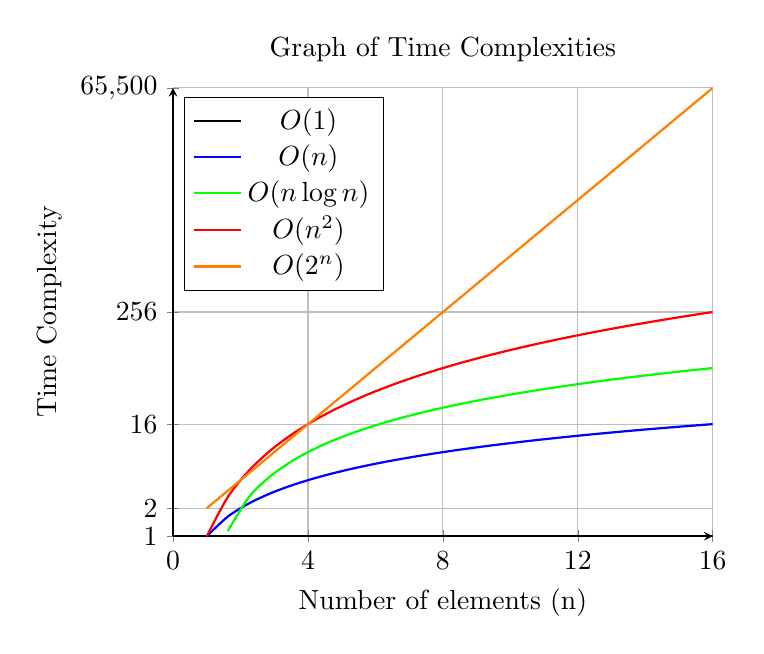
\begin{tikzpicture}
\begin{axis}[
    title={Graph of Time Complexities},
    xlabel={Number of elements (n)},
    ylabel={Time Complexity},
    domain=1:16,
    ymode=log,
    log basis y={2},
    ymin=1,
    ymax=65536,
    xtick={0,4,8,12,16},
    ytick={1,2,16,256,65536},
    log ticks with fixed point,
    axis lines = left,
    grid=both,
    smooth,
    legend style={at={(0.02,0.98)}, anchor=north west}
]
% Constant O(1)
\addplot [
    thick,
    color=black,
    domain=0:16,
] {1};
\addlegendentry{\(O(1)\)}

% Linear O(n)
\addplot [
    thick,
    color=blue,
] {x};
\addlegendentry{\(O(n)\)}

% Linearithmic O(n log n)
\addplot [
    thick,
    color=green,
] {x*log2(x)};
\addlegendentry{\(O(n \log n)\)}

% Quadratic O(n^2)
\addplot [
    thick,
    color=red,
] {x^2};
\addlegendentry{\(O(n^2)\)}

% Exponential O(2^n)
\addplot [
    thick,
    color=orange,
] {2^x};
\addlegendentry{\(O(2^n)\)}
\end{axis}
\end{tikzpicture}


\paragraph{Big Omega Notation}
Big Omega (\(\Omega\)) notation provides a lower bound on the time complexity of an algorithm, meaning it describes the best-case scenario. For an algorithm with time complexity \(T(n)\), if \(T(n) = \Omega(f(n))\), then there exists a constant \(c > 0\) and an input size \(n_0\) such that for all \(n \geq n_0\), \(T(n) \geq c \cdot f(n)\).

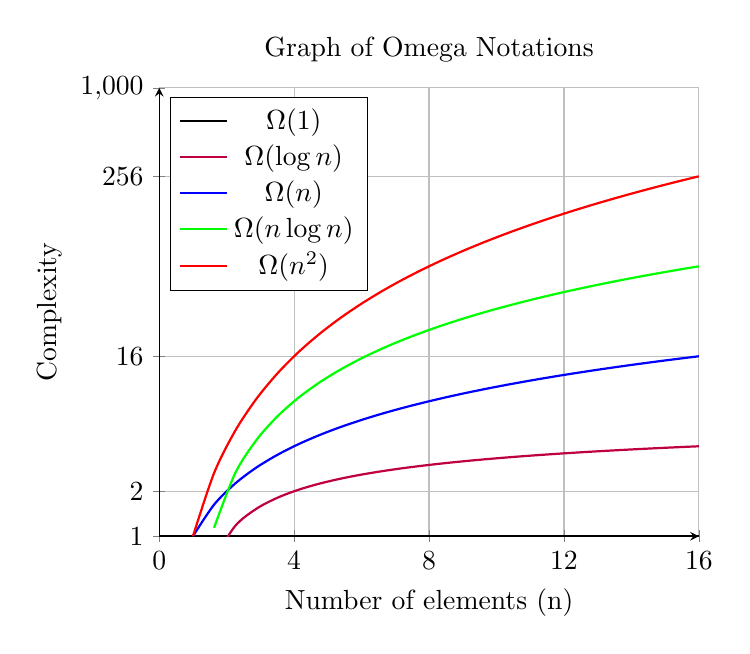
\begin{tikzpicture}
\begin{axis}[
    title={Graph of Omega Notations},
    xlabel={Number of elements (n)},
    ylabel={Complexity},
    domain=1:16,
    ymode=log,
    log basis y={2},
    ymin=1,
    ymax=1000,
    xtick={0,4,8,12,16},
    ytick={1,2,16,256,1000},
    log ticks with fixed point,
    axis lines = left,
    grid=both,
    smooth,
    legend style={at={(0.02,0.98)}, anchor=north west}
]
% Constant Omega(1)
\addplot [
    thick,
    color=black,
    domain=0:16,
] {1};
\addlegendentry{\(\Omega(1)\)}

% Logarithmic Omega(log n)
\addplot [
    thick,
    color=purple,
] {log2(x)};
\addlegendentry{\(\Omega(\log n)\)}

% Linear Omega(n)
\addplot [
    thick,
    color=blue,
] {x};
\addlegendentry{\(\Omega(n)\)}

% Linearithmic Omega(n log n)
\addplot [
    thick,
    color=green,
] {x*log2(x)};
\addlegendentry{\(\Omega(n \log n)\)}

% Quadratic Omega(n^2)
\addplot [
    thick,
    color=red,
] {x^2};
\addlegendentry{\(\Omega(n^2)\)}
\end{axis}
\end{tikzpicture}

\paragraph{Big Theta Notation}
Big Theta (\(\Theta\)) notation provides a tight bound on the time complexity, meaning it describes both the upper and lower bounds. For an algorithm with time complexity \(T(n)\), if \(T(n) = \Theta(f(n))\), then there exist constants \(c_1, c_2 > 0\) and an input size \(n_0\) such that for all \(n \geq n_0\), \(c_1 \cdot f(n) \leq T(n) \leq c_2 \cdot f(n)\).

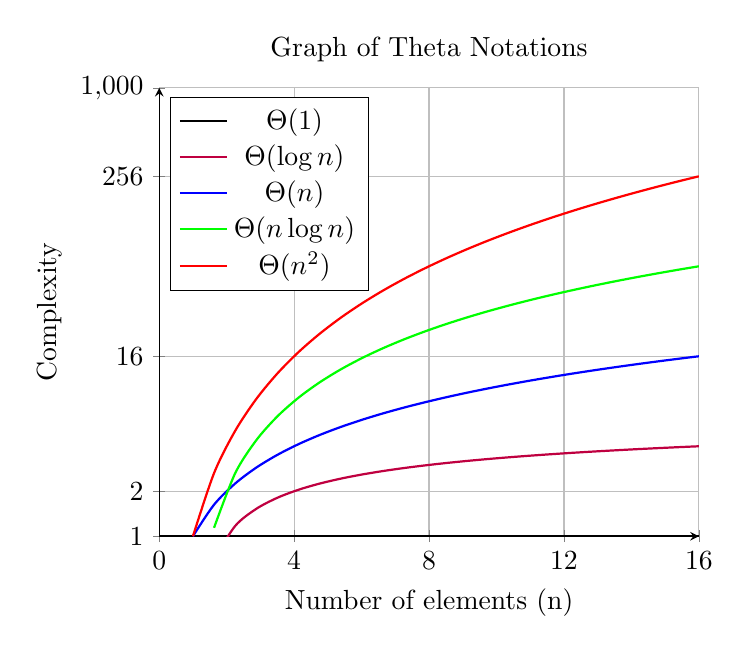
\begin{tikzpicture}
\begin{axis}[
    title={Graph of Theta Notations},
    xlabel={Number of elements (n)},
    ylabel={Complexity},
    domain=1:16,
    ymode=log,
    log basis y={2},
    ymin=1,
    ymax=1000,
    xtick={0,4,8,12,16},
    ytick={1,2,16,256,1000},
    log ticks with fixed point,
    axis lines = left,
    grid=both,
    smooth,
    legend style={at={(0.02,0.98)}, anchor=north west}
]
% Constant Theta(1)
\addplot [
    thick,
    color=black,
    domain=0:16,
] {1};
\addlegendentry{\(\Theta(1)\)}

% Logarithmic Theta(log n)
\addplot [
    thick,
    color=purple,
] {log2(x)};
\addlegendentry{\(\Theta(\log n)\)}

% Linear Theta(n)
\addplot [
    thick,
    color=blue,
] {x};
\addlegendentry{\(\Theta(n)\)}

% Linearithmic Theta(n log n)
\addplot [
    thick,
    color=green,
] {x*log2(x)};
\addlegendentry{\(\Theta(n \log n)\)}

% Quadratic Theta(n^2)
\addplot [
    thick,
    color=red,
] {x^2};
\addlegendentry{\(\Theta(n^2)\)}
\end{axis}
\end{tikzpicture}

\subsubsection{Space Complexity}
Space complexity measures the amount of memory an algorithm uses relative to the input size. It is crucial for understanding the memory requirements of an algorithm.

For instance, the space complexity of the Merge Sort algorithm is \(O(n)\) because it requires additional space to store the subarrays.

\subsection{Algorithmic Strategies}
Various algorithmic strategies can be employed to solve problems efficiently. These include divide and conquer, dynamic programming, greedy algorithms, and backtracking.

\subsubsection{Divide and Conquer}
Divide and conquer is a strategy that breaks a problem into smaller subproblems, solves each subproblem recursively, and combines their solutions. An example is Merge Sort, which divides the array, sorts each half, and merges the sorted halves.

\subsubsection{Dynamic Programming}
Dynamic programming solves problems by breaking them down into simpler subproblems and storing the results to avoid redundant calculations. 

\subsubsection{Greedy Algorithms}
Greedy algorithms make locally optimal choices at each step with the hope of finding a globally optimal solution. An example is the activity selection problem, where the goal is to select the maximum number of non-overlapping activities.

\subsubsection{Backtracking}
Backtracking involves exploring all possible solutions to a problem and abandoning solutions that do not satisfy the problem constraints. 


Understanding these algorithmic strategies is essential for designing effective solutions to a wide range of computational problems.

\FloatBarrier

\section{Designing and Analyzing Algorithms}
Designing and analyzing algorithms are fundamental skills in computer science. This section covers problem-solving techniques, the representation of algorithms using pseudocode, and methods for analyzing algorithm performance.

\subsection{Problem Solving and Algorithm Design}
Algorithm design starts with understanding the problem at hand. The key steps in problem solving and algorithm design include:

\begin{itemize}
    \item \textbf{Problem Definition:} Clearly define the problem, including inputs, outputs, and constraints.
    \item \textbf{Breaking Down the Problem:} Decompose the problem into smaller, more manageable subproblems.
    \item \textbf{Designing the Algorithm:} Develop a step-by-step procedure to solve the problem. This involves choosing the appropriate algorithmic strategy (e.g., divide and conquer, dynamic programming).
    \item \textbf{Implementation:} Translate the algorithm into a programming language.
    \item \textbf{Testing and Verification:} Ensure the algorithm works correctly by testing it with various inputs.
\end{itemize}

\subsection{Pseudocode and Algorithm Representation}
Pseudocode is a high-level description of an algorithm that combines natural language and programming constructs. It is used to represent algorithms in a way that is easy to understand and implement.

Pseudocode typically includes:
\begin{itemize}
    \item \textbf{Sequential Steps:} Instructions are written in a logical sequence.
    \item \textbf{Control Structures:} Includes loops (for, while) and conditionals (if, else).
    \item \textbf{Data Manipulation:} Operations on variables and data structures (arrays, lists).
\end{itemize}

\begin{algorithm}
\caption{Pseudocode Example: Binary Search}
\begin{algorithmic}[1]
\Procedure{BinarySearch}{A, n, key}
\State \textbf{Input:} Sorted array \(A\) of size \(n\), search key
\State \textbf{Output:} Index of key in \(A\) or \texttt{-1} if not found
\State $low \leftarrow 0$
\State $high \leftarrow n - 1$
\While{$low \leq high$}
    \State $mid \leftarrow \lfloor (low + high) / 2 \rfloor$
    \If{$A[mid] = key$}
        \State \Return $mid$
    \ElsIf{$A[mid] < key$}
        \State $low \leftarrow mid + 1$
    \Else
        \State $high \leftarrow mid - 1$
    \EndIf
\EndWhile
\State \Return -1
\EndProcedure
\end{algorithmic}
\end{algorithm}

\subsection{Algorithm Analysis}
Analyzing an algorithm involves determining its efficiency in terms of time and space complexity. This helps in understanding the algorithm's performance and scalability.

\subsubsection{Best, Worst, and Average Case Analysis}
Algorithm analysis considers different scenarios:
\begin{itemize}
    \item \textbf{Best Case:} The scenario where the algorithm performs the minimum number of operations.
    \item \textbf{Worst Case:} The scenario where the algorithm performs the maximum number of operations.
    \item \textbf{Average Case:} The expected number of operations over all possible inputs.
\end{itemize}

For example, in the case of binary search:
\begin{itemize}
    \item \textbf{Best Case:} \(O(1)\) - The key is found at the first comparison.
    \item \textbf{Worst Case:} \(O(\log n)\) - The key is not found, or is found after the maximum number of comparisons.
    \item \textbf{Average Case:} \(O(\log n)\) - The expected number of comparisons to find the key.
\end{itemize}

\subsubsection{Asymptotic Notation}
Asymptotic notation describes the behavior of an algorithm as the input size grows. The common notations include:
\begin{itemize}
    \item \textbf{Big O Notation (\(O\)):} Represents the upper bound of the time complexity, describing the worst-case scenario.
    \item \textbf{Omega Notation (\(\Omega\)):} Represents the lower bound of the time complexity, describing the best-case scenario.
    \item \textbf{Theta Notation (\(\Theta\)):} Represents the tight bound, describing the exact growth rate of the algorithm.
\end{itemize}


Understanding these concepts is crucial for evaluating and improving algorithm performance.

\FloatBarrier



\section{Ethical Considerations in Algorithm Design}
Designing algorithms goes beyond technical efficiency; it requires careful consideration of ethical issues such as bias, fairness, privacy, and security. This section explores these critical aspects and how they influence the development and deployment of algorithms.

\subsection{Bias and Fairness in Algorithms}
Bias in algorithms can lead to unfair treatment of individuals or groups, especially in sensitive areas like hiring, lending, and law enforcement. Ensuring fairness in algorithms is essential to prevent discrimination and promote equality.

\textbf{Sources of Bias:}
\begin{itemize}
    \item \textbf{Training Data Bias:} Algorithms trained on biased data can perpetuate or even amplify existing biases.
    \item \textbf{Algorithmic Bias:} Design choices and underlying assumptions can introduce bias.
    \item \textbf{User Interaction Bias:} User behaviors and feedback loops can skew algorithmic outcomes.
\end{itemize}

\textbf{Mathematical Definition of Fairness:}
Fairness can be defined in various ways, including:
\begin{itemize}
    \item \textbf{Statistical Parity:} Ensuring equal probability of positive outcomes across different groups.
    \[
    P(\hat{Y} = 1 \mid A = a) = P(\hat{Y} = 1 \mid A = b)
    \]
    where \( \hat{Y} \) is the predicted outcome, and \( A \) represents different demographic groups.
    \item \textbf{Equal Opportunity:} Ensuring equal true positive rates across groups.
    \[
    P(\hat{Y} = 1 \mid Y = 1, A = a) = P(\hat{Y} = 1 \mid Y = 1, A = b)
    \]
\end{itemize}

\textbf{Case Study: Fairness in Hiring Algorithms}
Consider a hiring algorithm that predicts job performance based on historical hiring data. If the data reflects past discrimination, the algorithm may unfairly favor certain demographics.

\begin{algorithm}
\caption{Bias Mitigation in Hiring Algorithm}
\begin{algorithmic}[1]
\Procedure{MitigateBias}{Candidates}
\State \textbf{Input:} List of candidates with features and demographic attributes
\State \textbf{Output:} Fair ranking of candidates
\State Normalize features to remove demographic influence
\State Apply re-weighting to balance demographic groups
\State Train algorithm on balanced data
\State Evaluate fairness using statistical parity and equal opportunity metrics
\EndProcedure
\end{algorithmic}
\end{algorithm}

\FloatBarrier

\subsection{Privacy and Security}
Algorithms often handle sensitive data, making privacy and security paramount. Protecting user data from unauthorized access and ensuring that algorithms do not inadvertently leak information is crucial.

\textbf{Privacy-Preserving Techniques:}
\begin{itemize}
    \item \textbf{Differential Privacy:} Ensures that the inclusion or exclusion of a single data point does not significantly affect the output.
    \[
    P(A(D)) \leq e^{\epsilon} P(A(D'))
    \]
    where \( D \) and \( D' \) are datasets differing by one element, and \( \epsilon \) controls the privacy loss.
    \item \textbf{Secure Multi-Party Computation (SMPC):} Allows parties to jointly compute a function over their inputs while keeping those inputs private.
\end{itemize}

\textbf{Case Study: Privacy in Health Data Algorithms}
Healthcare algorithms analyze sensitive patient data to provide diagnostics and treatment recommendations. Ensuring privacy is critical to protect patient confidentiality.

\begin{algorithm}
\caption{Differential Privacy in Health Data Analysis}
\begin{algorithmic}[1]
\Procedure{AnalyzeHealthData}{PatientData}
\State \textbf{Input:} Patient data with sensitive attributes
\State \textbf{Output:} Aggregated health insights
\State Apply noise to data using differential privacy mechanisms
\State Perform analysis on the sanitized data
\State Ensure results meet privacy thresholds
\EndProcedure
\end{algorithmic}
\end{algorithm}

\FloatBarrier

In conclusion, ethical considerations in algorithm design are essential to ensure that algorithms are fair, unbiased, and respectful of user privacy and security. Addressing these issues involves employing various techniques and continually evaluating the ethical implications of algorithmic decisions.


\section{Challenges and Future Directions in Algorithm Research}
Algorithm research is a dynamic field, constantly evolving to meet new challenges and opportunities. This section explores the key challenges in scalability and performance, the interdisciplinary applications of algorithms, and the emerging trends shaping the future of algorithm development.

\subsection{Scalability and Performance Issues}
Scalability and performance are critical considerations in algorithm design. As data sizes and computational demands grow, algorithms must efficiently handle large-scale problems without significant performance degradation.

\textbf{Key Challenges:}
\begin{itemize}
    \item \textbf{Data Volume:} Managing and processing vast amounts of data require algorithms that can scale linearly or sub-linearly with input size.
    \item \textbf{Computational Complexity:} Reducing time and space complexity to improve algorithm efficiency.
    \item \textbf{Resource Constraints:} Optimizing algorithms for limited computational resources, such as memory and processing power.
\end{itemize}

\subsection{Interdisciplinary Applications of Algorithms}
Algorithms are integral to a wide range of disciplines, driving advancements and solving complex problems across various fields.

\textbf{Key Areas:}
\begin{itemize}
    \item \textbf{Healthcare:} Algorithms analyze medical data for diagnosis, treatment planning, and predicting patient outcomes.
    \item \textbf{Finance:} Financial algorithms manage risks, optimize trading strategies, and detect fraud.
    \item \textbf{Environmental Science:} Algorithms model climate change, optimize resource management, and analyze ecological data.
    \item \textbf{Social Sciences:} Algorithms analyze social networks, study human behavior, and predict social trends.
\end{itemize}


\subsection{Emerging Trends in Algorithm Development}
The future of algorithm research is shaped by emerging trends that push the boundaries of what algorithms can achieve.

\textbf{Key Trends:}
\begin{itemize}
    \item \textbf{Artificial Intelligence and Machine Learning:} Algorithms are becoming more sophisticated, capable of learning and adapting from data.
    \item \textbf{Quantum Computing:} Quantum algorithms leverage quantum mechanics to solve problems exponentially faster than classical algorithms.
    \item \textbf{Blockchain and Cryptography:} Algorithms ensure secure transactions and data integrity in decentralized systems.
    \item \textbf{Edge Computing:} Algorithms process data closer to the source, reducing latency and improving real-time decision-making.
\end{itemize}

\textbf{Example: Quantum Algorithms}
Quantum algorithms, like Shor’s algorithm, solve complex problems such as integer factorization much faster than classical counterparts.

\begin{algorithm}
\caption{Shor's Algorithm for Integer Factorization}
\begin{algorithmic}[1]
\Procedure{ShorFactor}{N}
\State \textbf{Input:} Integer \( N \)
\State \textbf{Output:} Factors of \( N \)
\State Choose a random integer \( a \)
\State Compute \( \gcd(a, N) \)
\If{\(\gcd(a, N) \neq 1\)}
    \State \Return \(\gcd(a, N)\)
\EndIf
\State Find period \( r \) of \( a^x \mod N \)
\If{\(r\) is even and \(a^{r/2} \not\equiv -1 \mod N\)}
    \State \Return \(\gcd(a^{r/2} - 1, N)\) and \(\gcd(a^{r/2} + 1, N)\)
\EndIf
\EndProcedure
\end{algorithmic}
\end{algorithm}

\FloatBarrier

In conclusion, the field of algorithm research continues to evolve, addressing challenges of scalability, performance, and interdisciplinary applications, while embracing emerging trends that drive innovation and expand the horizons of what algorithms can accomplish.


\section{Practical Implementation of Algorithms}
Implementing algorithms effectively requires knowledge of programming languages, testing and debugging techniques, and performance optimization strategies. This section covers these crucial aspects, providing insights and examples to help you master algorithm implementation.

\subsection{Algorithm Implementation in Various Programming Languages}
Algorithms can be implemented in multiple programming languages, each with its own syntax and features. Understanding how to translate algorithmic logic into code is essential for practical application.

\textbf{Key Languages:}
\begin{itemize}
    \item \textbf{Python:} Known for its readability and extensive libraries, Python is a popular choice for implementing algorithms quickly and efficiently.
    \item \textbf{Java:} Java provides robustness and portability, making it suitable for large-scale applications.
    \item \textbf{C++:} Offers high performance and fine-grained control over system resources, ideal for resource-intensive algorithms.
\end{itemize}

\subsection{Testing and Debugging Algorithms}
Testing and debugging are critical to ensure that algorithms function correctly and efficiently. Proper testing helps identify and fix errors, while debugging pinpoints issues in the code.

\textbf{Testing Techniques:}
\begin{itemize}
    \item \textbf{Unit Testing:} Testing individual components or functions to ensure they work as expected.
    \item \textbf{Integration Testing:} Ensuring that different parts of the program work together correctly.
    \item \textbf{Regression Testing:} Verifying that new changes do not introduce new bugs.
\end{itemize}

\textbf{Debugging Techniques:}
\begin{itemize}
    \item \textbf{Print Statements:} Inserting print statements to track variable values and program flow.
    \item \textbf{Debugging Tools:} Using tools like gdb for C++, pdb for Python, or built-in debuggers in IDEs.
    \item \textbf{Code Reviews:} Having peers review code to catch errors and suggest improvements.
\end{itemize}

\subsection{Optimizing Algorithm Performance}
Optimizing algorithms involves refining their logic and implementation to improve efficiency. This can be achieved through various techniques and strategies.

\textbf{Optimization Techniques:}
\begin{itemize}
    \item \textbf{Time Complexity Reduction:} Choosing or redesigning algorithms to minimize their time complexity.
    \item \textbf{Space Complexity Reduction:} Reducing the memory footprint of algorithms.
    \item \textbf{Parallelization:} Distributing tasks across multiple processors to speed up execution.
    \item \textbf{Algorithm-Specific Optimizations:} Tailoring optimizations to specific algorithms, such as memoization in dynamic programming.
\end{itemize}

In summary, practical algorithm implementation involves selecting appropriate programming languages, thoroughly testing and debugging, and optimizing performance. Mastering these aspects ensures that algorithms are not only correct but also efficient and scalable in real-world applications.


\section{Conclusion}
The exploration of algorithms reveals their foundational role in technology and their pervasive impact on various aspects of society. This section recaps the key points discussed and highlights the broader implications of algorithms on technology and society.

\subsection{Recap of Key Points}
Throughout this document, we have covered essential aspects of algorithms, including their theoretical foundations, design, practical implementation, and ethical considerations. Here are the key takeaways:

\begin{itemize}
    \item \textbf{Understanding Algorithms:} We defined algorithms and discussed core concepts such as complexity and efficiency. We highlighted the importance of studying algorithms to solve real-world problems efficiently.
    \item \textbf{Theoretical Foundations:} We delved into basic algorithmic structures (sequences, selections, iterations) and explored complexity (time and space) and algorithmic strategies (divide and conquer, dynamic programming, greedy algorithms, backtracking).
    \item \textbf{Designing and Analyzing Algorithms:} We discussed problem-solving techniques, pseudocode representation, and various methods for analyzing algorithm performance, including best, worst, and average-case analysis.
    \item \textbf{Ethical Considerations:} We emphasized the need to address bias, fairness, privacy, and security in algorithm design to ensure ethical applications.
    \item \textbf{Challenges and Future Directions:} We explored scalability and performance issues, interdisciplinary applications, and emerging trends in algorithm development.
    \item \textbf{Practical Implementation:} We covered implementing algorithms in different programming languages, testing and debugging techniques, and optimizing performance for real-world applications.
\end{itemize}

\subsection{The Impact of Algorithms on Technology and Society}
Algorithms are the driving force behind numerous technological advancements, influencing various fields and transforming societal functions.

\textbf{Technological Impact:}
\begin{itemize}
    \item \textbf{Data Science and Machine Learning:} Algorithms enable the extraction of insights from large datasets, powering predictive analytics, recommendation systems, and automation.
    \item \textbf{Healthcare:} Algorithms enhance diagnostic accuracy, optimize treatment plans, and improve patient outcomes through data-driven insights.
    \item \textbf{Finance:} Algorithms facilitate high-frequency trading, risk management, fraud detection, and personalized financial services.
    \item \textbf{Transportation:} Algorithms optimize routes, manage traffic, and enhance the efficiency of logistics and supply chains.
\end{itemize}

\textbf{Societal Impact:}
\begin{itemize}
    \item \textbf{Communication:} Algorithms power search engines, social media platforms, and communication tools, shaping how information is accessed and shared.
    \item \textbf{Privacy and Security:} Encryption algorithms protect sensitive information, ensuring secure communication and data storage.
    \item \textbf{Ethics and Fairness:} The design of fair and unbiased algorithms is crucial for ensuring equitable access to technology and preventing discrimination.
    \item \textbf{Policy and Regulation:} The societal impact of algorithms necessitates thoughtful policy-making and regulation to address ethical concerns and protect public interests.
\end{itemize}



\section{Further Reading and Resources}
For those interested in delving deeper into the world of algorithms, there are numerous resources available, including key papers, books, online tutorials, and open-source libraries.

\subsection{Key Papers and Books on Algorithms}
\begin{itemize}
    \item \textbf{Books:}
    \begin{itemize}
        \item \textit{Introduction to Algorithms} by Thomas H. Cormen, Charles E. Leiserson, Ronald L. Rivest, and Clifford Stein. This comprehensive book covers a wide range of algorithms and is often referred to as the "CLRS" book.
        \item \textit{The Art of Computer Programming} by Donald E. Knuth. A seminal work in computer science, this multi-volume series delves deeply into the analysis and design of algorithms.
        \item \textit{Algorithms} by Robert Sedgewick and Kevin Wayne. This book provides an in-depth look at various algorithms and includes numerous examples and exercises.
    \end{itemize}
    
    \item \textbf{Key Papers:}
    \begin{itemize}
        \item "A Polynomial Time Algorithm for the Two-Commodity Flow Problem" by Jack Edmonds and Richard M. Karp. This paper introduces polynomial-time algorithms for network flow problems.
        \item "Computers and Intractability: A Guide to the Theory of NP-Completeness" by Michael Garey and David S. Johnson. A foundational text on the theory of computational complexity.
        \item "No Free Lunch Theorems for Optimization" by David H. Wolpert and William G. Macready. This paper discusses the theoretical limits of optimization algorithms.
    \end{itemize}
\end{itemize}

\subsection{Online Tutorials and Courses}
\begin{itemize}
    \item \textbf{Coursera:} Offers courses like "Algorithms, Part I \& II" by Princeton University, which cover essential algorithms and data structures.
    \item \textbf{edX:} Provides courses such as "Algorithm Design and Analysis" by Microsoft, focusing on algorithmic problem-solving techniques.
    \item \textbf{Khan Academy:} Features comprehensive tutorials on basic algorithms and data structures, suitable for beginners.
    \item \textbf{YouTube Channels:} Channels like "mycodeschool" and "MIT OpenCourseWare" offer video lectures on various algorithm topics.
\end{itemize}

\subsection{Open-Source Libraries and Algorithm Implementations}
\begin{itemize}
    \item \textbf{NumPy and SciPy:} Essential libraries for scientific computing in Python, providing numerous algorithms for mathematical operations and optimizations.
    \item \textbf{TensorFlow and PyTorch:} Popular frameworks for machine learning that include implementations of various learning algorithms.
    \item \textbf{NetworkX:} A Python library for the creation, manipulation, and study of complex networks, featuring numerous graph algorithms.
    \item \textbf{Boost C++ Libraries:} A collection of peer-reviewed, open-source C++ libraries that include implementations of many algorithms and data structures.
    \item \textbf{Apache Commons:} A set of reusable Java components, including libraries for mathematics, collections, and various utilities.
\end{itemize}




\chapter{Algorithms Analysis}

\section{Introduction to Algorithm Analysis}

In computer science, \textbf{algorithm analysis} is key to understanding the computational complexity of algorithms. This analysis assesses how the time, storage, and other resources needed to execute an algorithm relate to the size of its input. It involves estimating how the time (time complexity) or memory (space complexity) scales with input size.

\subsection{Overview and Importance}

Analyzing an algorithm helps identify how efficient it is. Generally, efficiency is gauged by how slowly the resource requirements grow with input size. The analysis might consider the best, worst, and average case scenarios to comprehensively understand an algorithm's behavior under various conditions. Typically, the focus is on the worst-case scenario, unless specified otherwise, to ensure the algorithm performs adequately under all circumstances.

\textbf{Theoretical Foundations}

Algorithm analysis is part of the broader field of computational complexity theory, which theorizes about the resources any algorithm would need to solve a computational problem. This theoretical insight guides the search for efficient algorithms by highlighting promising approaches.

\textbf{Asymptotic Analysis}

Most commonly, algorithms are analyzed asymptotically—that is, their performance is estimated based on very large input sizes. This approach uses notations like Big O (\(O\)), Big-omega (\(\Omega\)), and Big-theta (\(\Theta\)) to express these estimates. For example, binary search has a time complexity of \(O(\log n)\), indicating it scales logarithmically with the input size \(n\).

\subsection{Definition and Objectives}

Defining what constitutes a 'step' in an algorithm is crucial for meaningful efficiency estimates. To reflect actual running times accurately, each step’s duration must be consistently bounded by a constant. However, assumptions must be carefully scrutinized—for instance, assuming that adding any two numbers takes constant time may not hold if numbers can grow very large.

\textbf{Model of Computation}

To get exact measures of an algorithm’s efficiency, we often rely on a specific model of computation, like a Turing machine. This model might assume that certain operations are executed in unit time. For example, in binary search, if each element lookup is considered to occur in unit time, then finding an element in a sorted list of \(n\) items will take at most \(\log_2(n) + 1\) time units.

\textbf{Conclusion}

Understanding the subtleties of algorithm analysis allows us to appreciate why and how some algorithms perform better than others and under what conditions. This foundational knowledge not only aids in designing new algorithms but also in optimizing existing ones, ensuring they are robust across different computational scenarios.

Two cost models are generally used~\cite{AhoHopcroft1974, Hromkovič2004, Ausiello1999, Wegener20, Tarjan1983}:
\begin{itemize}
    \item 
    \textbf{Uniform Cost Model}:
    The uniform cost model, also called unit-cost model (and similar variations), assigns a constant cost to every machine operation, regardless of the size of the numbers involved. 
    \newline
    Let's consider an example algorithm For finding the sum of elements in an array: 

    \begin{algorithm}[H]
    \caption{Sum of Array Elements}
    \begin{algorithmic}[1]
    \Function{sumArray}{$A, n$}
        \State $sum \gets 0$
        \For{$i \gets 1 \text{ to } n$}
            \State $sum \gets sum + A[i]$
        \EndFor
        \State \Return $sum$
    \EndFunction
    \end{algorithmic}
    \end{algorithm}

    In this algorithm, each iteration of the \texttt{For} loop takes the same amount of time as it performs a constant number of operations. Therefore, the uniform cost model assumes each operation in the loop has uniform cost.

    \item 
    \textbf{Logarithmic Cost Model}:
    The logarithmic cost model, also called logarithmic-cost measurement (and similar variations), assigns a cost to every machine operation proportional to the number of bits involved. 
    \newline
    Let's consider the example of the binary search algorithm:

    \begin{algorithm}[H]
    \caption{Binary Search}
    \begin{algorithmic}[1]
    \Function{binarySearch}{$A, key, low, high$}
        \If{$low \leq high$}
            \State $mid \gets \frac{low + high}{2}$
            \If{$A[mid] == key$}
                \State \Return $mid$
            \ElsIf{$A[mid] > key$}
                \State \Return \Call{binarySearch}{$A, key, low, mid-1$}
            \Else
                \State \Return \Call{binarySearch}{$A, key, mid+1, high$}
            \EndIf
        \EndIf
        \State \Return $-1$
    \EndFunction
    \end{algorithmic}
    \end{algorithm}

    In binary search, the input size is divided in half at each step, leading to a logarithmic number of steps to find the desired element. Therefore, the cost of the algorithm is logarithmic in the input size.
\end{itemize}

The latter is more cumbersome to use, so it is only employed when necessary, For example in the analysis of arbitrary-precision arithmetic algorithms, like those used in cryptography.

A key point which is often overlooked is that published lower bounds For problems are often given For a model of computation that is more restricted than the set of operations that you could use in practice and therefore there are algorithms that are faster than what would naively be thought possible~\cite{PriceAbstraction}.

\subsection{The Role of Algorithm Analysis in Software Development}

Algorithm analysis plays a crucial role in software development by providing a theoretical framework to estimate the run-time efficiency of algorithms as the input size grows. This analysis is vital because the execution time of a program can vary widely—from seconds to years—based on the algorithm it uses.

\textbf{Run-Time Analysis}

Run-time analysis helps predict how the time it takes to execute an algorithm will change with increasing input size, denoted as \(n\). While software profiling offers practical run-time measurements, it cannot cover all possible inputs. Theoretical run-time analysis fills this gap, allowing developers to anticipate performance across all scenarios.

\subsection{Overview of Complexity Measures}

Complexity measures provide a way to quantify the growth rate of an algorithm's run-time or space requirements relative to the input size.

\textbf{Understanding Growth Rates}

The run-time of an algorithm might be bounded by a function \(f(n)\), such that for any sufficiently large input \(n\) and a constant \(c\), the run-time does not exceed \(c \times f(n)\). This bounding function helps in categorizing algorithms according to their efficiency and scalability.

\textbf{Big O Notation}

Big O notation is a common tool used to describe these upper bounds, simplifying the comparison of algorithms by focusing on their worst-case scenarios. For instance, insertion sort is described as \(O(n^2)\) because its run-time grows quadratically with the input size. Similarly, while quicksort typically runs in \(O(n \log n)\), its worst-case scenario is \(O(n^2)\).

\textbf{Application in Software Development}

Understanding these complexity measures is essential for developers when selecting or designing algorithms, particularly for applications where performance and resource utilization are critical. By applying algorithm analysis, developers can ensure that their software is both efficient and scalable, avoiding algorithms that perform poorly with large datasets.

In summary, the study of algorithm complexity and run-time analysis not only enhances the theoretical knowledge of computer science but also has direct applications in the practical world of software development. By mastering these concepts, developers can make informed choices about which algorithms to implement in different scenarios, leading to more efficient and effective software solutions.


Consider the following Insertion Sort related example:\newline
Insertion sort is a simple sorting algorithm that builds the final sorted array one element at a time. It iterates through an array and at each iteration, it removes one element from the input data and finds its correct position within the sorted part of the array.

\begin{algorithm}
\caption{Insertion Sort}
\begin{algorithmic}[1]
\Procedure{InsertionSort}{$A, n$}
    \For{$i \gets 1$ to $n$}
        \State $key \gets A[i]$
        \State $j \gets i - 1$
        \While{$j \geq 0$ and $A[j] > key$}
            \State $A[j + 1] \gets A[j]$
            \State $j \gets j - 1$
        \EndWhile
        \State $A[j + 1] \gets key$
    \EndFor
\EndProcedure
\end{algorithmic}
\end{algorithm}

Let $T(n)$ represent the worst-case run-time of insertion sort For an input of size $n$. In each iteration of the outer loop, insertion sort compares the key with the elements in the sorted subarray and shIfts larger elements one position to the right until the correct position For the key is found. 

Considering the worst-case scenario, when the array is in reverse order, insertion sort would perform maximum comparisons and shifts in each iteration. In the worst case, For each $i$ from $2$ to $n$, insertion sort performs $i-1$ comparisons and shifts.

Hence, the worst-case run-time $T(n)$ can be expressed as:
$$ T(n) = \sum_{i=2}^{n} (i - 1) = 1 + 2 + 3 + \dots + (n-1) = \frac{n(n-1)}{2} = O(n^2) $$




\subsection{Evaluating run-time complexity}

The run-time complexity For the worst-case scenario of a given algorithm can sometimes be evaluated by examining the structure of the algorithm and making some simplifying assumptions.  Consider the following pseudocode:

\begin{verbatim}
 1    get a positive integer n from input
 2    If n > 10
 3        print "This might take a While..."
 4    For i = 1 to n
 5        For j = 1 to i
 6            print i * j
 7    print "Done!"
\end{verbatim}

A given computer will take a discrete amount of time to execute each of the instructions involved with carrying out this algorithm.  Say that the actions carried out in step 1 are considered to consume time at most $T_1$, step 2 uses time at most $T_2$, and so Forth.

In the algorithm above, steps 1, 2, and 7 will only be run once.  For a worst-case evaluation, it should be assumed that step 3 will be run as well.  Thus the total amount of time to run steps 1-3 and step 7 is:

\[
T_1 + T_2 + T_3 + T_7.
\]

The loops in steps 4, 5, and 6 are trickier to evaluate.  The outer loop test in step 4 will execute $(n + 1)$ times\footnote{an extra step is required to terminate the For loop, hence $n + 1$ and not $n$ executions}, which will consume $T_4(n + 1)$ time.  The inner loop, on the other hand, is governed by the value of $j$, which iterates from 1 to $i$.  On the first pass through the outer loop, $j$ iterates from 1 to 1:  The inner loop makes one pass, so running the inner loop body (step 6) consumes $T_6$ time, and the inner loop test (step 5) consumes $2T_5$ time.  During the next pass through the outer loop, $j$ iterates from 1 to 2:  the inner loop makes two passes, so running the inner loop body (step 6) consumes $2T_6$ time, and the inner loop test (step 5) consumes $3T_5$ time.

Altogether, the total time required to run the inner loop body can be expressed as an arithmetic progression:

\[
T_6 + 2T_6 + 3T_6 + \cdots + (n-1) T_6 + n T_6
\]

which can be factored\footnote{It can be proven by induction that $1 + 2 + 3 + \cdots + (n-1) + n = \frac{n(n+1)}{2}$} as

\[
\left[ 1 + 2 + 3 + \cdots + (n-1) + n \right] T_6 = \left[ \frac{1}{2} (n^2 + n) \right] T_6
\]

The total time required to run the inner loop \emph{test} can be evaluated similarly:

\begin{align}
& 2T_5 + 3T_5 + 4T_5 + \cdots + (n-1) T_5 + n T_5 + (n + 1) T_5\\
=&\ T_5 + 2T_5 + 3T_5 + 4T_5 + \cdots + (n-1)T_5 + nT_5 + (n+1)T_5 - T_5
\end{align}

which can be factored as

\begin{align}
& T_5 \left[ 1+2+3+\cdots + (n-1) + n + (n + 1) \right] - T_5 \\
=& \left[ \frac{1}{2} (n^2 + n) \right] T_5 + (n + 1)T_5 - T_5 \\
=& \left[ \frac{1}{2} (n^2 + n) \right] T_5 + n T_5 \\
=& \left[ \frac{1}{2} (n^2 + 3n) \right] T_5
\end{align}

Therefore, the total run-time For this algorithm is:

\[
f(n) = T_1 + T_2 + T_3 + T_7 + (n + 1)T_4 + \left[ \frac{1}{2} (n^2 + n) \right] T_6 + \left[ \frac{1}{2} (n^2+3n) \right] T_5
\]

which reduces to

\[
f(n) = \left[ \frac{1}{2} (n^2 + n) \right] T_6 + \left[ \frac{1}{2} (n^2 + 3n) \right] T_5 + (n + 1)T_4 + T_1 + T_2 + T_3 + T_7
\]

As a rule-of-thumb, one can assume that the highest-order term in any given function dominates its rate of growth and thus defines its run-time order.  In this example, $n^2$ is the highest-order term, so one can conclude that $f(n) = O(n^2)$.  Formally this can be proven as follows:

\begin{quote}
Prove that $\left[ \frac{1}{2} (n^2 + n) \right] T_6 + \left[ \frac{1}{2} (n^2 + 3n) \right] T_5 + (n + 1)T_4 + T_1 + T_2 + T_3 + T_7 \le cn^2,\ n \ge n_0$

\begin{align}
%\[
&\left[ \frac{1}{2} (n^2 + n) \right] T_6 + \left[ \frac{1}{2} (n^2 + 3n) \right] T_5 + (n + 1)T_4 + T_1 + T_2 + T_3 + T_7\\
\le &( n^2 + n )T_6 + ( n^2 + 3n )T_5 + (n + 1)T_4 + T_1 + T_2 + T_3 + T_7 \ (\text{For } n \ge 0 )
%\]
\end{align}


Let $k$ be a constant greater than or equal to $[T_1..T_7]$

\begin{align}
&T_6( n^2 + n ) + T_5( n^2 + 3n ) + (n + 1)T_4 + T_1 + T_2 + T_3 + T_7 \nonumber\\
&\le k( n^2 + n ) + k( n^2 + 3n ) + kn + 5k \nonumber\\
&= 2kn^2 + 5kn + 5k \nonumber\\
&\le 2kn^2 + 5kn^2 + 5kn^2 + 5kn \nonumber\\
&\le 12kn^2
\end{align}
For $n \ge 1$.

Therefore, $f(n) = O(n^2)$.
\end{quote}

\section{Understanding Complexity Notations}
In theoretical analysis of algorithms, it is common to estimate their complexity in the asymptotic sense, i.e., to estimate the complexity function For arbitrarily large input. Big O notation, Big Omega (\(\Omega\)) notation, and Big Theta (\(\Theta\)) notation are used to this end. For instance, binary search is said to run in a number of steps proportional to the logarithm of the size $n$ of the sorted list being searched, or in $O(\log n)$, colloquially 'in logarithmic time'. Usually asymptotic estimates are used because different implementations of the same algorithm may differ in efficiency. However, the efficiencies of any two 'reasonable' implementations of a given algorithm are related by a constant multiplicative factor called a 'hidden constant'.

\subsection{The Big O Notation}
\subsubsection{Definition and Significance}

Big O notation is a mathematical notation that describes the limiting behavior of a function when the argument tends towards a particular value or infinity. In the context of algorithm analysis, Big O notation is used to describe the upper bound on the growth rate of an algorithm's time or space complexity. It provides a standardized and concise way to express the efficiency of algorithms by focusing on their worst-case performance.

The significance of Big O notation lies in its ability to provide a clear understanding of how an algorithm scales with input size. By analyzing the upper bound of an algorithm's complexity, engineers and developers can make informed decisions about algorithm selection and optimization strategies. Additionally, Big O notation facilitates communication and comparison between different algorithms, enabling the identification of the most efficient solutions For specific problem domains.

\subsubsection{Basic Examples}

To illustrate the concept of Big O notation, consider the following basic examples:

\begin{itemize}
    \item \textbf{Constant Time}: An algorithm that performs a single operation regardless of the input size has a time complexity of O(1). For example, accessing an element in an array by index or checking If a number is even or odd.
    \FloatBarrier
    Consider the following algorithm:
    \FloatBarrier
    \begin{algorithm}
\caption{Access Element in Array}
\begin{algorithmic}[1]
\Function{AccessElement}{$arr, index$}
    \State \textbf{Return} $arr[index]$
\EndFunction
\end{algorithmic}
\end{algorithm}
\FloatBarrier
    \item \textbf{Linear Time}: An algorithm whose runtime grows linearly with the input size has a time complexity of O(n). For example, iterating through each element in an array or list.
    \FloatBarrier
    Following is the algorithmic example:
\FloatBarrier
\begin{algorithm}[H]
\caption{Example Algorithm For Big O Notation}
\begin{algorithmic}
\State function foo($n$)
\State $sum = 0$
\For{$i = 1$ to $n$}
\State $sum = sum + i$
\EndFor
\State Return $sum$
\end{algorithmic}
\end{algorithm}
\FloatBarrier
The time complexity of this algorithm is $O(n)$ because the loop runs $n$ times, resulting in a linear growth rate with respect to the input size $n$.
    \FloatBarrier
    \item \textbf{Quadratic Time}: An algorithm whose runtime grows quadratically with the input size has a time complexity of O($n^2$). For example, nested loops where each iteration depends on the size of the input.
    \FloatBarrier
    Following is the algorithmic example:
    \FloatBarrier
    \begin{algorithm}
\caption{Nested Loop}
\begin{algorithmic}[1]
\Function{NestedLoop}{$n$}
    \For{$i \gets 1$ to $n$}
        \For{$j \gets 1$ to $n$}
            \State Perform some operation
        \EndFor
    \EndFor
\EndFunction
\end{algorithmic}
\end{algorithm}
\FloatBarrier
\end{itemize}






\subsection{The Big Omega (\(\Omega\)) Notation}

\subsubsection{Definition and Significance}

Big Omega notation is another mathematical notation used in algorithm analysis. It describes the lower bound on the growth rate of an algorithm's time or space complexity. Essentially, Big Omega notation provides information about the best-case scenario For the algorithm's performance. Unlike Big O notation, which represents the upper bound on the growth rate, Big Omega notation focuses on the lower bound, indicating the minimum amount of resources required by the algorithm.

The significance of Big Omega notation lies in its ability to provide insights into the inherent efficiency of an algorithm. By analyzing the lower bound of an algorithm's complexity, engineers and developers can gain a better understanding of its best-case performance and identify situations where the algorithm performs optimally. Additionally, Big Omega notation complements Big O notation by offering a more comprehensive view of an algorithm's behavior across different input sizes.

\subsubsection{Basic Examples}

To illustrate the concept of Big Omega notation, consider the following basic examples:

\begin{itemize}
    \item \textbf{Linear Time}: An algorithm whose runtime grows linearly with the input size has a lower bound time complexity of $\Omega(n)$. For example, a linear search algorithm always requires at least one comparison For each element in the input array.
    \FloatBarrier
Consider the following algorithm:
\FloatBarrier
\begin{algorithm}[H]
\caption{Example Algorithm For Big Omega (\(\Omega\)) Notation}
\begin{algorithmic}
\State function bar($n$)
\State $min = A[1]$
\For{$i = 2$ to $n$}
\If{$A[i] < min$}
\State $min = A[i]$
\EndIf
\EndFor
\State Return $min$
\end{algorithmic}
\end{algorithm}
\FloatBarrier
The time complexity of this algorithm is $\Omega(n)$ because in the best-case scenario, the algorithm needs to iterate through the array once to find the minimum value, resulting in a linear growth rate.
    
    \item \textbf{Quadratic Time}: An algorithm whose runtime grows quadratically with the input size has a lower bound time complexity of $\Omega(n^2)$. For example, an algorithm that computes all pairs of elements in an input array requires at least quadratic time to complete.
    \FloatBarrier
    Following is the algorithmic example:
    \FloatBarrier
    \begin{algorithm}
\caption{Quadratic Time Algorithm}
\begin{algorithmic}[1]
\Function{QuadraticTime}{$A, n$}
    \State $result \gets 0$
    \For{$i \gets 1$ to $n$}
        \For{$j \gets 1$ to $n$}
            \State $result \gets result + A[i] \times A[j]$
        \EndFor
    \EndFor
    \State \textbf{Return} $result$
\EndFunction
\end{algorithmic}
\end{algorithm}
\end{itemize}

\subsection{The Big Theta (\(\Theta\)) Notation}

\subsubsection{Definition and Significance}

Big Theta (\(\Theta\)) notation is a mathematical notation used in algorithm analysis. It provides both the upper and lower bounds on the growth rate of an algorithm's time or space complexity. Unlike Big O and Big Omega notations, which represent only the upper and lower bounds respectively, Big Theta notation represents the tightest bound on the algorithm's performance. This notation is often used when the upper and lower bounds are equal, indicating that the algorithm's performance behaves consistently across different input sizes.

The significance of Big Theta notation lies in its ability to precisely describe the behavior of an algorithm. By providing both upper and lower bounds, Big Theta notation offers a clear understanding of the algorithm's performance characteristics and helps in determining its efficiency in the worst-case, best-case, and average-case scenarios.

\subsubsection{Understanding the tight bound}

In Big Theta (\(\Theta\)) notation, the upper and lower bounds on an algorithm's performance are equal, indicating a tight bound on its growth rate. This implies that the algorithm's time or space complexity grows at the same rate regardless of the input size. In other words, the algorithm's behavior is consistent and predictable, making Big Theta notation particularly useful For analyzing algorithms with well-defined performance characteristics.


\subsubsection{Basic Examples}

To illustrate the concept of Big Theta notation, consider the following basic examples:

\begin{itemize}
    \item \textbf{Linear Time}: An algorithm whose runtime grows linearly with the input size has a time complexity of \(\Theta(n)\). For example, a linear search algorithm typically performs \(n\) comparisons in the worst-case scenario, where \(n\) is the size of the input array.
    \FloatBarrier
    Consider the following algorithm:
\FloatBarrier
\begin{algorithm}[H]
\caption{Example Algorithm For Big Theta (\(\Theta\)) Notation}
\begin{algorithmic}
\State function baz($n$)
\State $sum = 0$
\For{$i = 1$ to $n$}
\State $sum = sum + i$
\EndFor
\For{$j = 1$ to $n$}
\State $sum = sum + j$
\EndFor
\State Return $sum$
\end{algorithmic}
\end{algorithm}
\FloatBarrier
The time complexity of this algorithm is $\Theta(n)$ because it consists of two loops, each running $n$ times. As a result, the algorithm has a linear growth rate that matches both the lower and upper bounds.
\FloatBarrier
    \item \textbf{Quadratic Time}: An algorithm whose runtime grows quadratically with the input size has a time complexity of \(\Theta(n^2)\). For example, an algorithm that computes all pairs of elements in an input array performs \(\frac{n \times (n-1)}{2}\) operations, where \(n\) is the size of the input array.
    \FloatBarrier
    Following is the algorithmic example:
    \FloatBarrier
    \begin{algorithm}
\caption{Quadratic Time Algorithm}
\begin{algorithmic}[1]
\Function{QuadraticTime}{$A, n$}
    \State $result \gets 0$
    \For{$i \gets 1$ to $n$}
        \For{$j \gets 1$ to $n$}
            \State $result \gets result + A[i] \times A[j]$
        \EndFor
    \EndFor
    \State \textbf{Return} $result$
\EndFunction
\end{algorithmic}
\end{algorithm}
\end{itemize}

\subsection{Comparison of the Three Notations}

When comparing Big O, Big Omega (\(\Omega\)), and Big Theta (\(\Theta\)) notations, it is important to understand their relationships. Big O notation provides an upper bound on the growth rate of a function, Big Omega (\(\Omega\))notation provides a lower bound, and Big Theta (\(\Theta\)) notation provides a tight bound. In many cases, these notations are used together to provide a comprehensive analysis of an algorithm's performance.


In summary:
\begin{itemize}
    \item Big O notation: Upper bound
    \item Big Omega (\(\Omega\)) notation: Lower bound
    \item Big Theta (\(\Theta\)) notation: Tight bound
\end{itemize}

\section{Analytical Tools For Algorithm Analysis}

Analytical tools play a crucial role in analyzing the performance and efficiency of algorithms. They provide us with a quantifiable way to understand how algorithms behave under different scenarios. In this section, we will discuss some fundamental analytical tools For algorithm analysis.

\subsection{Asymptotic Analysis}

Asymptotic analysis is a method used to evaluate the performance of an algorithm as the input size tends towards infinity. It helps us understand how the algorithm will scale with larger inputs.

\subsubsection{Growth of Functions}

In asymptotic analysis, we focus on the growth rates of functions that represent the running time or space complexity of algorithms. Common growth rates include constant time, logarithmic time, linear time, quadratic time, etc.

\subsubsection{Common Asymptotic Functions}

Some common asymptotic functions used in algorithm analysis include:
\begin{itemize}
  \item $O(\cdot)$ - Big O notation For the upper bound of a function.
  \item $\Omega(\cdot)$ - Omega notation For the lower bound of a function.
  \item $\Theta(\cdot)$ - Theta notation For tight bounds of a function.
\end{itemize}

\subsection{Recurrence Relations}

Recurrence relations are equations that describe the runtime of a recursive algorithm in terms of its subproblem sizes. Solving these recurrences helps us analyze the time complexity of recursive algorithms.

\subsubsection{Solving Recurrences}

There are various methods to solve recurrence relations, such as substitution method, master theorem, recursion tree method, etc. explained as follows:
\FloatBarrier
Substitution Method:
\FloatBarrier
The substitution method is a technique used to solve recurrence relations by making an educated guess and then proving the correctness of the guess using mathematical induction. Here's how it works:

\begin{enumerate}
    \item \textbf{Guess a solution}: We make an educated guess about the Form of the solution to the recurrence relation. This guess often involves an expression involving the size of the input and some unknown constants.
    
    \item \textbf{Prove by induction}: We then prove the correctness of our guess using mathematical induction. This involves verifying that the guessed solution satisfies the original recurrence relation and its initial conditions.
    
    \item \textbf{Example}:
    
    Let's consider the recurrence relation For the Fibonacci sequence:
    
    \[
    T(n) = T(n-1) + T(n-2)
    \]
    
    where \(T(n)\) represents the time complexity of computing the \(n\)-th Fibonacci number. By guessing that \(T(n) = O(2^n)\), we can prove by induction that this guess is correct.
\end{enumerate}
\FloatBarrier
Master Theorem:
\FloatBarrier

The master theorem is a powerful tool For solving recurrence relations that arise in the analysis of divide-and-conquer algorithms. It provides a straightForward way to determine the asymptotic behavior of the solution without the need For guesswork or induction. The master theorem applies to recurrence relations of the Form \(T(n) = aT(n/b) + f(n)\), where \(a \geq 1\), \(b > 1\), and \(f(n)\) is a given function.

\begin{enumerate}
    \item \textbf{Identify the Form}: We start by identifying the Form of the recurrence relation and determining the values of \(a\), \(b\), and \(f(n)\).
    
    \item \textbf{Apply the master theorem}: Based on the values of \(a\), \(b\), and the Form of \(f(n)\), we can apply one of the cases of the master theorem to determine the asymptotic behavior of \(T(n)\).
    
    \item \textbf{Example}:
    
    Consider the recurrence relation \(T(n) = 2T(n/2) + n\). By identifying \(a = 2\), \(b = 2\), and \(f(n) = n\), we can apply case 2 of the master theorem, which tells us that \(T(n) = \Theta(n \log n)\).
\end{enumerate}
\FloatBarrier
Recursion Tree Method:
\FloatBarrier

The recursion tree method is a graphical technique used to visualize and solve recurrence relations. It involves drawing a tree diagram to represent the recursive calls made by the algorithm and then analyzing the structure of the tree to determine the overall time complexity.

\begin{enumerate}
    \item \textbf{Construct the recursion tree}: We start by drawing a tree diagram representing the recursive calls made by the algorithm. Each node in the tree corresponds to a subproblem, and the edges represent the recursive calls.
    
    \item \textbf{Analyze the tree}: We then analyze the structure of the tree to determine the total number of nodes and levels. By summing up the work done at each level of the tree, we can derive the overall time complexity of the algorithm.
    
    \item \textbf{Example}:
    
    Let's use the recursion tree method to analyze the time complexity of the merge sort algorithm. By constructing a recursion tree For merge sort, we can see that the height of the tree is \(\log n\), and each level of the tree requires \(O(n)\) work. Therefore, the overall time complexity of merge sort is \(O(n \log n)\).
\end{enumerate}

\subsection{Amortized Analysis}

Amortized analysis is a technique used to determine the average time complexity of a sequence of operations in data structures where some operations may be expensive but are offset by others that are relatively cheap.

\subsubsection{Definition and Applications}

Amortized analysis is a technique used to determine the average time complexity of a sequence of operations in data structures where some operations may be expensive but are offset by others that are relatively cheap. It provides a way to analyze the overall performance of data structures by averaging the cost of individual operations over a series of operations.
\FloatBarrier
\textbf{Conceptual Understanding:}
\FloatBarrier

The basic idea behind amortized analysis is to distribute the cost of expensive operations over multiple cheaper operations. This ensures that the average cost of operations remains low even If some individual operations are expensive. 

Consider a dynamic array that doubles its size whenever it runs out of space. Although resizing the array is an expensive operation, it occurs infrequently compared to the cheap constant-time operations of accessing or appending elements. Amortized analysis allows us to show that the average cost of resizing the array is low when spread across multiple append operations.

\FloatBarrier
\textbf{Algorithmic Example: Dynamic Array}
\FloatBarrier

Let's consider a dynamic array that doubles its size whenever it runs out of space. We'll use amortized analysis to analyze the average time complexity of appending \(n\) elements to the array.
\FloatBarrier
\begin{algorithm}
\caption{Append Operation on Dynamic Array}
\begin{algorithmic}[1]
\Function{Append}{$\text{array}, \text{element}$}
    \If{$\text{size}(\text{array}) = \text{capacity}(\text{array})$}
        \State \text{resize}($\text{array}, 2 \times \text{capacity}(\text{array})$)
    \EndIf
    \State $\text{array}[\text{size}(\text{array})] \gets \text{element}$
    \State $\text{size}(\text{array}) \gets \text{size}(\text{array}) + 1$
\EndFunction
\end{algorithmic}
\end{algorithm}
\FloatBarrier
In this example, resizing the array takes \(O(n)\) time, where \(n\) is the current size of the array. However, we can show that the amortized cost of each append operation is \(O(1)\) using the potential method.

\FloatBarrier
\textbf{Applications:}
\FloatBarrier
Amortized analysis is commonly used in the analysis of data structures and algorithms where the cost of individual operations varies signIficantly. Some common applications include:

\begin{itemize}
    \item \textbf{Dynamic arrays}: As demonstrated in the example above, amortized analysis helps in analyzing the average time complexity of dynamic array operations like appending elements.
    
    \item \textbf{Binary heaps}: Amortized analysis can be used to analyze the time complexity of heap operations such as insertion and deletion, where some operations may require restructuring the heap to maintain its properties.
    
    \item \textbf{Hash tables}: In hash tables, resizing the underlying array can be an expensive operation. Amortized analysis helps in analyzing the average time complexity of insertion and deletion operations, taking into account occasional resizing.
\end{itemize}

Overall, amortized analysis provides a useful tool For understanding the average performance of algorithms and data structures over a sequence of operations.

\section{Practical Analysis of Algorithms}
Analyzing algorithms is crucial in understanding their efficiency and performance. Practical analysis of algorithms involves studying their behavior, runtime complexity, and space complexity using mathematical and empirical techniques.
\subsection{Binary Search}
Binary search is a fundamental searching algorithm that efficiently locates a target value within a sorted array. It works by repeatedly dividing the search interval in half. The key to its efficiency lies in discarding half of the search space at each step.
\subsubsection{Algorithmic Description:}
\FloatBarrier
\begin{algorithm}
\caption{Binary Search}
\begin{algorithmic}[1]
\Function{BinarySearch}{$A[], n, x$}
\State $low \gets 0$
\State $high \gets n - 1$
\While{$low \leq high$}
    \State $mid \gets \lfloor(low + high) / 2 \rfloor$
    \If{$A[mid] == x$}
        \State \Return $mid$
    \ElsIf{$A[mid] < x$}
        \State $low \gets mid + 1$
    \Else
        \State $high \gets mid - 1$
    \EndIf
\EndWhile
\State \Return $-1$ \Comment{Element not found}
\EndFunction
\end{algorithmic}
\end{algorithm}
\FloatBarrier
This function takes a sorted array \texttt{arr} and a target value \texttt{target} as input and Returns the index of \texttt{target} in the array If found, otherwise Returns -1.
\subsubsection{Analysis and Time Complexity}
\textbf{Time Complexity Analysis}

To analyze the time complexity of binary search, let's denote the length of the input array as \(n\). In each iteration of the binary search algorithm, the search interval is divided in half. Therefore, the size of the search interval is reduced by a factor of 2 in each iteration.

Let \(k\) be the number of iterations required to find the target value or determine that it is not present in the array. Since the search interval size is halved in each iteration, we have:

\[
\frac{n}{2^k} = 1
\]

Solving For \(k\), we get \(k = \log_2 n\). Thus, the time complexity of binary search is \(O(\log n)\).

\textbf{Space Complexity Analysis}

Binary search is an in-place algorithm that does not require any additional memory proportional to the input size \(n\). Therefore, the space complexity of binary search is \(O(1)\).

Binary search is a highly efficient algorithm For finding elements in a sorted array, with a time complexity of \(O(\log n)\), making it suitable For large datasets where efficiency is crucial.

\subsection{Sorting Algorithms}
Sorting algorithms are crucial in arranging elements in a specific order. They are used in various applications like databases, search algorithms, and more. Different sorting algorithms have different time complexities, influencing their efficiency.

There are numerous sorting algorithms, each with its own advantages and disadvantages. Some of the commonly used sorting algorithms include:

\begin{itemize}
    \item \textbf{Bubble Sort}: Bubble sort repeatedly steps through the list, compares adjacent elements, and swaps them If they are in the wrong order. It continues until the list is sorted.

     Algorithmic Example For Bubble Sort:
     \FloatBarrier % Ensure algorithm appears after the paragraph
    \begin{algorithm}
\caption{Bubble Sort}
\begin{algorithmic}[1]
\Function{BubbleSort}{$A[]$}
    \State $n \gets$ length of $A$
    \For{$i \gets 0$ \textbf{to} $n-1$}
        \For{$j \gets 0$ \textbf{to} $n-i-1$}
            \If{$A[j] > A[j+1]$}
                \State Swap $A[j]$ and $A[j+1]$
            \EndIf
        \EndFor
    \EndFor
\EndFunction
\end{algorithmic}
\end{algorithm}
\FloatBarrier % Ensure algorithm appears after the paragraph

    \item \textbf{Selection Sort}: Selection sort divides the input list into two parts: the sorted sublist and the unsorted sublist. It repeatedly selects the minimum element from the unsorted sublist and moves it to the beginning of the sorted sublist.
    
    Algorithmic Example For Selection Sort:
     \FloatBarrier % Ensure algorithm appears after the paragraph
     \begin{algorithm}
\caption{Selection Sort}
\begin{algorithmic}[1]
\Function{SelectionSort}{$A[]$}
    \State $n \gets$ length of $A$
    \For{$i \gets 0$ \textbf{to} $n-1$}
        \State $min\_idx \gets i$
        \For{$j \gets i+1$ \textbf{to} $n$}
            \If{$A[j] < A[min\_idx]$}
                \State $min\_idx \gets j$
            \EndIf
        \EndFor
        \State Swap $A[min\_idx]$ and $A[i]$
    \EndFor
\EndFunction
\end{algorithmic}
\end{algorithm}
\FloatBarrier % Ensure algorithm appears after the paragraph
    
    \item \textbf{Insertion Sort}: Insertion sort builds the final sorted array one item at a time by repeatedly taking the next element from the unsorted part and inserting it into its correct position in the sorted part.
    
    Algorithmic Example For Insertion Sort:
     \FloatBarrier % Ensure algorithm appears after the paragraph
     \begin{algorithm}
\caption{Insertion Sort}
     \begin{algorithmic}[1]
\Function{Insertion Sort}{$A[]$}
    \State $n \gets$ length of $A$
    \For{$i \gets 1$ \textbf{to} $n-1$}
        \State $key \gets A[i]$
        \State $j \gets i - 1$
        \While{$j \geq 0$ and $A[j] > key$}
            \State $A[j + 1] \gets A[j]$
            \State $j \gets j - 1$
        \EndWhile
        \State $A[j + 1] \gets key$
    \EndFor
\EndFunction
\end{algorithmic}
\end{algorithm}
\FloatBarrier % Ensure algorithm appears after the paragraph
    
    \item \textbf{Merge Sort}: Merge sort follows the divide-and-conquer strategy. It divides the input array into two halves, sorts the two halves separately, and then merges them.

 Algorithmic Example For Merge Sort:
     \FloatBarrier % Ensure algorithm appears after the paragraph
\begin{algorithm}
\caption{Merge Sort}
\begin{algorithmic}[1]
\Function{MergeSort}{$A[], start, end$}
    \If{$start < end$}
        \State $mid \gets (start + end) // 2$
        \State \Call{MergeSort}{$A[], start, mid$}
        \State \Call{MergeSort}{$A[], mid+1, end$}
        \State \Call{Merge}{$A[], start, mid, end$}
    \EndIf
\EndFunction
\FloatBarrier % Ensure algorithm appears after the paragraph
\Function{Merge}{$A[], start, mid, end$}
    \State $n_1 \gets mid - start + 1$
    \State $n_2 \gets end - mid$
    \State Create temporary arrays $L[1 \dots n_1]$ and $R[1 \dots n_2]$
    \For{$i \gets 1$ \textbf{to} $n_1$}
        \State $L[i] \gets A[start + i - 1]$
    \EndFor
    \For{$j \gets 1$ \textbf{to} $n_2$}
        \State $R[j] \gets A[mid + j]$
    \EndFor
    \State $i \gets 1$, $j \gets 1$, $k \gets start$
    \While{$i \leq n_1$ and $j \leq n_2$}
        \If{$L[i] \leq R[j]$}
            \State $A[k] \gets L[i]$
            \State $i \gets i + 1$
        \Else
            \State $A[k] \gets R[j]$
            \State $j \gets j + 1$
        \EndIf
        \State $k \gets k + 1$
    \EndWhile
    \While{$i \leq n_1$}
        \State $A[k] \gets L[i]$
        \State $i \gets i + 1$, $k \gets k + 1$
    \EndWhile
    \While{$j \leq n_2$}
        \State $A[k] \gets R[j]$
        \State $j \gets j + 1$, $k \gets k + 1$
    \EndWhile
\EndFunction
\end{algorithmic}
\end{algorithm}
\FloatBarrier % Ensure algorithm appears after the paragraph
    \item \textbf{Quick Sort}: Quick sort also follows the divide-and-conquer strategy. It selects a pivot element and partitions the array into two subarrays such that elements less than the pivot are on the left and elements greater than the pivot are on the right. It then recursively sorts the subarrays.

Algorithmic Example For Quick Sort:
     \FloatBarrier % Ensure algorithm appears after the paragraph
    \begin{algorithm}
\caption{Quick Sort}
\begin{algorithmic}[1]
\Function{QuickSort}{$A[], start, end$}
    \If{$start < end$}
        \State $pivot \gets$ Partition($A[], start, end$)
        \State \Call{QuickSort}{$A[], start, pivot-1$}
        \State \Call{QuickSort}{$A[], pivot+1, end$}
    \EndIf
\EndFunction
\FloatBarrier % Ensure algorithm appears after the paragraph
\Function{Partition}{$A[], start, end$}
    \State $pivot \gets A[end]$
    \State $i \gets start - 1$
    \For{$j \gets start$ \textbf{to} $end-1$}
        \If{$A[j] < pivot$}
            \State $i \gets i + 1$
            \State Swap $A[i]$ and $A[j]$
        \EndIf
    \EndFor
    \State Swap $A[i + 1]$ and $A[end]$
    \State \Return $i + 1$
\EndFunction
\end{algorithmic}
\end{algorithm}

    \FloatBarrier % Ensure algorithm appears after the paragraph
    \item \textbf{Heap Sort}: Heap sort builds a heap data structure from the input array and repeatedly extracts the maximum element from the heap and rebuilds the heap until the array is sorted.
    Algorithmic Example For Heap Sort:
     \FloatBarrier % Ensure algorithm appears after the paragraph
     \begin{algorithm}
\caption{Heap Sort}
\begin{algorithmic}[1]
\Function{HeapSort}{$A[]$}
    \State BuildMaxHeap($A[]$)
    \For{$i \gets$ length of $A$ down to $2$}
        \State Swap $A[1]$ and $A[i]$
        \State Heapify($A[], 1, i-1$)
    \EndFor
\EndFunction
\FloatBarrier % Ensure algorithm appears after the paragraph
\Function{BuildMaxHeap}{$A[]$}
    \State $n \gets$ length of $A$
    \For{$i \gets n // 2$ down to $1$}
        \State Heapify($A[], i, n$)
    \EndFor
\EndFunction
\FloatBarrier % Ensure algorithm appears after the paragraph
\Function{Heapify}{$A[], i, n$}
    \State $largest \gets i$
    \State $l \gets 2i$
    \State $r \gets 2i + 1$
    \If{$l \leq n$ and $A[l] > A[largest]$}
        \State $largest \gets l$
    \EndIf
    \If{$r \leq n$ and $A[r] > A[largest]$}
        \State $largest \gets r$
    \EndIf
    \If{$largest \neq i$}
        \State Swap $A[i]$ and $A[largest]$
        \State Heapify($A[], largest, n$)
    \EndIf
\EndFunction
\end{algorithmic}
\end{algorithm}
\end{itemize}
\FloatBarrier % Ensure algorithm appears after the paragraph
\subsubsection{Complexity Analysis of the sorting algorithms}

The space and time complexity of sorting algorithms varies depending on the algorithm used and the input data. Here are the average and worst-case time complexities along with the space complexities of some common sorting algorithms:

\begin{itemize}
    \item \textbf{Bubble Sort}: 
    \begin{itemize}
        \item \textbf{Time Complexity: }$O(n^2)$
        \item \textbf{Space Complexity: }Bubble sort is an in-place comparison-based sorting algorithm. It only requires a constant amount of additional space For storing temporary variables. Therefore, the space complexity of bubble sort is \(O(1)\).
    \end{itemize}
    
    \item \textbf{Selection Sort}: 
    \begin{itemize}
        \item \textbf{Time Complexity: }$O(n^2)$
        \item \textbf{Space Complexity: }Similar to bubble sort, selection sort is an in-place comparison-based sorting algorithm. It also requires only a constant amount of additional space For storing temporary variables. Hence, the space complexity of selection sort is \(O(1)\).
        \end{itemize}
    
    \item \textbf{Insertion Sort}: 
    \begin{itemize}
        \item \textbf{Time Complexity: }$O(n^2)$
        \item \textbf{Space Complexity: }Insertion sort is another in-place comparison-based sorting algorithm. Like bubble sort and selection sort, it requires only a constant amount of additional space For storing temporary variables. Therefore, the space complexity of insertion sort is \(O(1)\).
        \end{itemize}
    
    \item \textbf{Merge Sort}:
    \begin{itemize}
        \item \textbf{Time Complexity: }$O(n \log n)$
        \item \textbf{Space Complexity: }Merge sort is a divide-and-conquer sorting algorithm that requires additional space For the merge operation. During the merging phase, it needs space to store the merged subarrays temporarily. The space complexity of merge sort is \(O(n)\), where \(n\) is the size of the input array.
        \end{itemize}
          
    
    \item \textbf{Quick Sort}: 
    \begin{itemize}
        \item \textbf{Time Complexity: }$O(n \log n)$ (average case), $O(n^2)$ (worst case)
        \item \textbf{Space Complexity: }Quick sort is another divide-and-conquer sorting algorithm that operates in-place. However, it typically requires additional space For the recursive function calls in the call stack. The worst-case space complexity of quick sort is \(O(n)\), where \(n\) is the size of the input array. In the average case, the space complexity is \(O(\log n)\).
        \end{itemize}
    \item \textbf{Heap Sort}:
    \begin{itemize}
        \item \textbf{Time Complexity: }$O(n \log n)$
        \item \textbf{Space Complexity: }Heap sort is an in-place comparison-based sorting algorithm that uses a binary heap data structure. It does not require any additional space beyond the input array size For storing temporary variables. Therefore, the space complexity of heap sort is \(O(1)\).
        \end{itemize}
\end{itemize}
\FloatBarrier
\textbf{Choosing the Right Sorting Algorithm}

The choice of sorting algorithm depends on various factors such as the size of the input data, the distribution of data, memory constraints, and stability requirements. It is important to analyze these factors to select the most appropriate sorting algorithm For a given scenario.



\subsection{Graph Algorithms}
In computer engineering, graph algorithms are a set of techniques used to solve problems involving graphs. A graph is a collection of nodes (vertices) and edges that connect pairs of nodes. Graph algorithms can be broadly classified into two categories: traversal algorithms and path finding algorithms.

\subsubsection{Traversal Algorithms}

Traversal algorithms are used to visit or traverse all the nodes in a graph. The two most common traversal algorithms are depth-first search (DFS) and breadth-first search (BFS).
\begin{itemize}
    \item Depth-First Search (DFS):

Depth-first search explores as far as possible along each branch before backtracking. It starts at a selected node (the root) and explores as far as possible along each branch before backtracking.
\FloatBarrier
\begin{algorithm}
\caption{Depth-first Search (DFS)}
\begin{algorithmic}[1]
\Function{DFS}{$G, v, visited[]$}
    \State $visited[v] \gets \text{True}$
    \State \textbf{print} $v$
    \For{$u$ \textbf{in} $G.adjacentVertices(v)$}
        \If{$\neg visited[u]$}
            \State \Call{DFS}{$G, u, visited$}
        \EndIf
    \EndFor
\EndFunction
\end{algorithmic}
\end{algorithm}
\FloatBarrier

\item Breadth-First Search (BFS):

Breadth-first search explores all the neighboring nodes at the present depth before moving on to the nodes at the next depth level. It starts at a selected node (the root) and explores all of the neighbor nodes at the present depth before moving on to the nodes at the next depth level.
\FloatBarrier % Ensure algorithm appears after the paragraph
\begin{algorithm}
\caption{Breadth-first Search (BFS)}
\begin{algorithmic}[1]
\Function{BFS}{$G, start$}
    \State $visited[start] \gets \text{True}$
    \State $queue \gets [start]$
    \While{$queue$ is not empty}
        \State $v \gets$ dequeue from $queue$
        \State \textbf{print} $v$
        \For{$u$ \textbf{in} $G.adjacentVertices(v)$}
            \If{$\neg visited[u]$}
                \State $visited[u] \gets \text{True}$
                \State enqueue $u$ into $queue$
            \EndIf
        \EndFor
    \EndWhile
\EndFunction
\end{algorithmic}
\end{algorithm}
\FloatBarrier

\end{itemize}
\FloatBarrier % Ensure algorithm appears after the paragraph
\subsubsection{Pathfinding Algorithms}

Pathfinding algorithms are used to find the shortest path between two nodes in a graph. The most common pathfinding algorithm is Dijkstra's algorithm.
\FloatBarrier % Ensure algorithm appears after the paragraph
\begin{itemize}
\item Dijkstra's Algorithm:
Dijkstra's algorithm finds the shortest path between a starting node and all other nodes in the graph. 
\FloatBarrier % Ensure algorithm appears after the paragraph
\begin{algorithm}
\caption{Dijkstra's Algorithm}
\begin{algorithmic}[1]
\Function{Dijkstra}{$G, source$}
    \State $dist \gets$ dictionary of distances initialized to $\infty$ For all vertices
    \State $dist[source] \gets 0$
    \State $pq \gets$ priority queue initialized with $(0, source)$
    \While{$pq$ is not empty}
        \State $d, v \gets$ dequeue from $pq$
        \If{$d > dist[v]$}
            \State \textbf{continue}
        \EndIf
        \For{$u, w$ \textbf{in} $G.adjacentVertices(v)$}
            \State $new\_dist \gets dist[v] + w$
            \If{$new\_dist < dist[u]$}
                \State $dist[u] \gets new\_dist$
                \State enqueue $(new\_dist, u)$ into $pq$
            \EndIf
        \EndFor
    \EndWhile
\EndFunction
\end{algorithmic}
\end{algorithm}
\FloatBarrier

\end{itemize}
\FloatBarrier % Ensure algorithm appears after the paragraph

\section{Case Studies in Algorithm Analysis}
In algorithm analysis, three commonly used paradigms are \textit{Divide and Conquer Algorithms}, \textit{Dynamic Programming}, and \textit{Greedy Algorithms}.

\subsection{Divide and Conquer Algorithms}
Divide and Conquer Algorithms involve breaking down a problem into smaller subproblems, solving these subproblems recursively, and then combining the solutions to solve the original problem. The typical structure of a Divide and Conquer Algorithm includes three steps:
\begin{itemize}
  \item \textbf{Divide:} Break the problem into smaller subproblems.
  \item \textbf{Conquer:} Solve the subproblems recursively.
  \item \textbf{Combine:} Merge the solutions of the subproblems to solve the original problem.
\end{itemize}


\subsection{Dynamic Programming}
Dynamic Programming is a method For solving complex problems by breaking them down into simpler subproblems. It involves solving each subproblem only once and storing their solutions to avoid redundant computations. The key idea in Dynamic Programming is to use the solutions of overlapping subproblems.
\subsubsection{Analysis of Fibonacci Sequence Calculation}
A classic example of Dynamic Programming is the \textit{Fibonacci Sequence}. The Fibonacci Sequence can be efficiently computed using Dynamic Programming by storing the solutions to subproblems. The time complexity of the Dynamic Programming solution For the Fibonacci Sequence is $O(n)$.

The Fibonacci sequence is a series of numbers where each number is the sum of the two preceding ones, usually starting with 0 and 1. The sequence starts as follows: 0, 1, 1, 2, 3, 5, 8, 13, 21, ...

\paragraph{Algorithm}

The following algorithm uses dynamic programming to compute the $n^{th}$ Fibonacci number:
\FloatBarrier % Ensure algorithm appears after the paragraph
\begin{algorithm}
\caption{Fibonacci Sequence with Dynamic Programming}
\begin{algorithmic}[1]
\Procedure{Fibonacci}{$n$}
    \State Initialize an array $fib$ of size $n+1$
    \State $fib[0] \gets 0$, $fib[1] \gets 1$
    \For{$i \gets 2$ \textbf{to} $n$}
        \State $fib[i] \gets fib[i-1] + fib[i-2]$
    \EndFor
    \State \textbf{Return} $fib[n]$
\EndProcedure
\end{algorithmic}
\end{algorithm}
\FloatBarrier % Ensure algorithm appears after the paragraph
\paragraph{Explanation}

The algorithm computes the Fibonacci numbers iteratively using dynamic programming. It starts by initializing an array $fib$ of size $n+1$ to store the Fibonacci numbers.

The base cases are initialized as $fib[0] = 0$ and $fib[1] = 1$. Then, For each $i$ from $2$ to $n$, the algorithm calculates $fib[i]$ as the sum of the two preceding Fibonacci numbers, $fib[i-1]$ and $fib[i-2]$.

By iteratively computing and storing Fibonacci numbers, the algorithm avoids redundant calculations and improves efficiency.

\paragraph{Time Complexity}

The time complexity of the algorithm is $O(n)$, as it iterates through the array once to compute each Fibonacci number.
\paragraph{Space Complexity}
The space complexity of the given Fibonacci function can be analyzed as follows:

\begin{itemize}
    \item The function initializes a list `fib` of size `n + 1`, which requires space proportional to the input size `n`.
    \item Therefore, the space complexity of the algorithm is \(O(n)\), as it uses additional space linearly dependent on the input size.
\end{itemize}

\subsection{Greedy Algorithms}
Greedy Algorithms make a series of choices based on a specific criterion at each step with the hope of finding an optimal solution. At each step, a greedy algorithm selects the best available option without considering future consequences. Greedy Algorithms do not always guarantee an optimal solution, but they often provide a good approximation.

An example of a Greedy Algorithm is the \textit{Fractional Knapsack Problem}. In this problem, items with weights and values are given, and the goal is to maximize the total value of items that can be fit into a knapsack of limited capacity. The algorithm selects items based on their value-to-weight ratio in a greedy manner.
In the Fractional Knapsack Problem, we are given a set of items, each with a weight $w_i$ and a value $v_i$, and a knapsack that can hold a maximum weight $W$. The objective is to maximize the total value of the items that can be placed into the knapsack without exceeding its weight capacity.

\subsubsection{Greedy Approach}

The greedy approach to solving the Fractional Knapsack Problem involves selecting items based on their value-to-weight ratio. At each step, we choose the item with the highest value-to-weight ratio and add as much of it as possible to the knapsack. This process is repeated until the knapsack is full or there are no more items left to consider.
\FloatBarrier % Ensure algorithm appears after the paragraph
\begin{algorithm}
\caption{Fractional Knapsack}
\begin{algorithmic}[1]
\Procedure{FractionalKnapsack}{$\text{items}, W$}
    \State Sort items by value-to-weight ratio in non-increasing order
    \State Initialize total value $V$ to $0$
    \State Initialize remaining capacity $C$ to $W$
    \For{each item $i$ in items}
        \If{$w_i \leq C$}
            \State Add item $i$ completely to the knapsack
            \State Update $V$ by adding $v_i$
            \State Update $C$ by subtracting $w_i$
        \Else
            \State Add a fraction of item $i$ to the knapsack
            \State Update $V$ by adding fraction of $v_i$
            \State Update $C$ to $0$
            \State Break
        \EndIf
    \EndFor
    \State \textbf{Return} $V$ \Comment{Total value of items in knapsack}
\EndProcedure
\end{algorithmic}
\end{algorithm}
\FloatBarrier % Ensure algorithm appears after the paragraph
\paragraph{Mathematical Detail}

Let $n$ be the number of items.

\begin{itemize}
    \item The time complexity of the sorting step is $O(n \log n)$.
    \item The loop iterates over all $n$ items, each requiring $O(1)$ time For comparisons.
    \item Therefore, the overall time complexity of the algorithm is $O(n \log n)$.
\end{itemize}

Let $V_{\text{opt}}$ be the optimal value that can be achieved.

The greedy algorithm may not always produce the optimal solution. However, it does guarantee a solution that is at least a fraction of the optimal solution. Let $V_{\text{greedy}}$ be the value obtained using the greedy algorithm.

\begin{itemize}
    \item Since the algorithm selects items based on their value-to-weight ratio, it ensures that each item contributes the maximum possible value For its weight.
    \item Thus, the value obtained by the greedy algorithm is at least $\frac{1}{2}$ times the optimal value, i.e., $V_{\text{greedy}} \geq \frac{1}{2} V_{\text{opt}}$.
\end{itemize}
\FloatBarrier % Ensure algorithm appears after the paragraph

\subsubsection{Kruskal's and Prim's Algorithms For Minimum Spanning Tree}

Kruskal's and Prim's algorithms are two popular greedy algorithms used to find the minimum spanning tree (MST) of a connected, undirected graph. 

\paragraph{Kruskal's Algorithm}

Kruskal's algorithm builds the MST by iteratively adding the smallest edge that does not Form a cycle until all vertices are connected.
\FloatBarrier
\begin{algorithm}
\caption{Kruskal's Algorithm}
\begin{algorithmic}[1]
\Function{Kruskal}{$G$}
    \State $T \gets \emptyset$ \Comment{Initialize empty MST}
    \State Sort edges of $G$ by weight
    \For{each edge $(u, v)$ in $G$ in sorted order}
        \If{$(u, v)$ does not create a cycle in $T$}
            \State Add $(u, v)$ to $T$
        \EndIf
    \EndFor
    \State \Return $T$
\EndFunction
\end{algorithmic}
\end{algorithm}

\FloatBarrier
\textbf{Example:} Consider the following graph $G$ with vertices $V = \{A, B, C, D, E\}$ and edges $E = \{(A, B, 5), (A, C, 3), (B, C, 1), (B, D, 4), (C, D, 2), (C, E, 6), (D, E, 7)\}$. Applying Kruskal's algorithm on $G$ results in the MST $T = \{(B, C, 1), (C, D, 2), (A, C, 3), (B, D, 4), (C, E, 6)\}$.

\paragraph{Prim's Algorithm}

Prim's algorithm grows the MST from a single vertex, iteratively adding the smallest edge connected to the current MST until all vertices are included.
\FloatBarrier
\begin{algorithm}
\caption{Prim's Algorithm}
\begin{algorithmic}[1]
\Function{Prim}{$G$}
    \State $T \gets \emptyset$ \Comment{Initialize empty MST}
    \State Choose a starting vertex $s$
    \State Initialize priority queue $Q$ with all vertices and keys $\infty$
    \State Set key of $s$ to 0
    \While{$Q$ is not empty}
        \State $u \gets$ Extract-Min($Q$)
        \For{each vertex $v$ adjacent to $u$}
            \If{$v$ is in $Q$ and weight of edge $(u, v)$ is less than key of $v$}
                \State Update key of $v$ to weight of edge $(u, v)$
                \State Update parent of $v$ to $u$
            \EndIf
        \EndFor
        \State Add edge $(u, \text{parent}[u])$ to $T$
    \EndWhile
    \State \Return $T$
\EndFunction
\end{algorithmic}
\end{algorithm}

\FloatBarrier
\textbf{Example:} Using Prim's algorithm on the same graph $G$ yields the MST $T = \{(A, C, 3), (B, C, 1), (C, D, 2), (B, D, 4), (C, E, 6)\}$.



\section{Advanced Topics in Algorithmic Analysis}
\subsection{Randomized Algorithms:}

Randomized algorithms are a fascinating class of algorithms that introduce randomness into their execution process. Unlike deterministic algorithms, which follow a predefined sequence of steps to produce the same output For a given input, randomized algorithms incorporate randomness in their decision-making process. This randomness could be introduced through sources such as random number generators or probabilistic techniques.

One of the primary motivations For using randomized algorithms is their ability to provide efficient solutions to problems where deterministic algorithms may struggle due to their time complexity or complexity of design. By making random choices during execution, randomized algorithms can often achieve better average-case performance or simplify the problem-solving process.

The applications of randomized algorithms span a wide range of fields, including cryptography, machine learning, optimization problems, and computational biology, among others.
\FloatBarrier
\subsubsection{Randomized Quick Sort and Hashing}
\paragraph{Randomized QuickSort}

Randomized QuickSort is a randomized version of the QuickSort algorithm that randomly chooses a pivot element to partition the input array. This random choice helps in avoiding the worst-case time complexity of QuickSort.

Algorithm:
\FloatBarrier
\begin{algorithm}
\caption{Randomized QuickSort}
\begin{algorithmic}[1]
\State Array $A$, Indices $low$, $high$
\Function{randomizedQuickSort}{$A, low, high$}
    \If{$low < high$}
        \State $pivot \gets \text{random}(low, high)$
        \State $pivot \gets \text{partition}(A, low, high, pivot)$
        \State \textsc{randomizedQuickSort}($A, low, pivot-1$)
        \State \textsc{randomizedQuickSort}($A, pivot+1, high$)
    \EndIf
\EndFunction
\end{algorithmic}
\end{algorithm}
\FloatBarrier

Despite their advantages, randomized algorithms also present challenges, such as the need to analyze their probabilistic behavior and ensure correctness in all possible scenarios. Analyzing the performance of randomized algorithms often involves probabilistic reasoning and statistical techniques to estimate their expected behavior over a range of inputs.
\FloatBarrier
\paragraph{Hashing in Randomized Algorithms}

Hashing is a technique used to efficiently store and retrieve data in a data structure called a hash table. In the context of randomized algorithms, hashing involves mapping keys to indices in a hash table using a hash function. Randomized algorithms often use hashing For tasks such as maintaining sets, performing dictionary lookups, or implementing caches.

\paragraph{Hash Function}

A hash function is a function that takes a key as input and produces an index (hash value) in the hash table. It should distribute keys uniFormly across the table to minimize collisions (two keys hashing to the same index). A good hash function has the following properties:

\begin{itemize}
    \item \textbf{Deterministic:} Given the same input key, the hash function should produce the same output index.
    \item \textbf{UniFormity:} The hash function should evenly distribute keys across the hash table, reducing the likelihood of collisions.
    \item \textbf{Efficiency:} The hash function should be computationally efficient to calculate.
\end{itemize}

\paragraph{Collision Resolution}

Collisions occur when two keys hash to the same index in the hash table. There are various techniques to handle collisions, including:

\begin{itemize}
    \item \textbf{Chaining:} Each slot in the hash table contains a linked list of key-value pairs that hash to the same index.
    \item \textbf{Open Addressing:} In case of a collision, an alternative slot in the hash table is found using a probing sequence.
    \item \textbf{Double Hashing:} A second hash function is used to calculate the step size For probing, reducing clustering.
\end{itemize}

\paragraph{Algorithmic Example: Insertion with Chaining}

Let's consider an algorithm For inserting a key-value pair into a hash table using chaining For collision resolution:

\begin{algorithm}
\caption{Insertion with Chaining}
\begin{algorithmic}[1]
\Function{Insert}{$\text{hash\_table}, key, value$}
    \State $index \gets \text{hash\_function}(key)$
    \State Create a new node with key-value pair: $(key, value)$
    \State Append the node to the linked list at index $index$ in $\text{hash\_table}$
\EndFunction
\end{algorithmic}
\end{algorithm}

In this algorithm, the hash function maps the key to an index in the hash table. Then, a new node containing the key-value pair is inserted at the end of the linked list at the corresponding index.


\subsection{Parallel Algorithms:}

Parallel algorithms represent a pivotal paradigm in contemporary computing, harnessing the power of multiple processing units to enhance computational efficiency. As computing systems evolve with the proliferation of multi-core processors and distributed environments, the significance of parallel algorithms becomes increasingly pronounced, facilitating concurrent execution of tasks and leveraging resources optimally.

One of the primary motivations behind parallel algorithms is to mitigate the inherent limitations of sequential processing, where tasks are executed sequentially, one after the other. By distributing the workload across multiple processing units, parallel algorithms enable tasks to be executed concurrently, thereby reducing overall execution time and improving system throughput.

Parallel algorithms find widespread applications across various domains, including scientific computing, data analytics, artificial intelligence, and simulations. 
\subsubsection{Parallel Algorithm For Matrix Multiplication}
\FloatBarrier
Parallel matrix multiplication involves breaking down the matrix multiplication task into subtasks that can be computed in parallel across multiple processing units.
\FloatBarrier
\paragraph{Algorithm:}
\FloatBarrier

\begin{algorithm}
\caption{Parallel Matrix Multiplication}
\begin{algorithmic}
\Require{Matrices $A$ ($m \times n$), $B$ ($n \times p$)}

\Function{parallelMatrixMult}{$A, B$}
    \State $C \gets \text{initialize}(m \times p)$
    \For{$i$ from $1$ to $m$ in parallel}
        \For{$j$ from $1$ to $p$ in parallel}
            \For{$k$ from $1$ to $n$}
                \State $C[i][j] \mathrel{+}= A[i][k] \cdot B[k][j]$
            \EndFor
        \EndFor
    \EndFor
\EndFunction
\end{algorithmic}
\end{algorithm}
\FloatBarrier
Designing efficient parallel algorithms involves addressing several challenges, including load balancing, synchronization, communication overhead, and scalability. Effective parallelization requires careful consideration of algorithmic design, data partitioning strategies, and parallel execution models to achieve optimal performance across diverse computing architectures.

In conclusion, parallel algorithms represent a cornerstone of modern computing, enabling efficient utilization of computational resources and scalability across diverse application domains. As computing systems continue to evolve with the advent of multi-core processors, accelerators, and distributed architectures, the importance of parallel algorithms in driving computational advancements and addressing complex challenges will continue to grow.


\subsection{Approximation Algorithms:}

Approximation algorithms represent a powerful approach to solving optimization problems when finding an exact solution is prohibitively expensive or impractical. These algorithms trade off computational complexity For efficiency by providing solutions that are near-optimal within a guaranteed approximation factor. By sacrificing optimality For speed, approximation algorithms enable the rapid solution of complex optimization problems in various fields, including computer science, operations research, and engineering.

The versatility of approximation algorithms makes them indispensable in scenarios where exact solutions are either unattainable or require excessive computational resources.

\subsubsection{Travelling Salesman Problem and Vertex Cover}
\paragraph{Travelling Salesman Problem}
The Travelling Salesman Problem (TSP) is a classic optimization problem in which the goal is to find the shortest possible route that visits each city exactly once and Returns to the original city. It is a well-known NP-hard problem, meaning that there is no known polynomial-time algorithm that can solve it optimally For all instances. However, there exist approximation algorithms that provide near-optimal solutions within a guaranteed approximation factor.

One such approximation algorithm For the TSP is the Nearest Neighbor Algorithm. The algorithm starts at a random city and repeatedly selects the nearest unvisited city until all cities have been visited. Finally, it Returns to the starting city, completing the tour. Although the Nearest Neighbor Algorithm does not guarantee the optimal solution, it often produces solutions that are relatively close to the optimal.

\textbf{Algorithmic Example: Nearest Neighbor Algorithm For TSP}

\begin{algorithm}
\caption{Nearest Neighbor Algorithm For TSP}
\begin{algorithmic}[1]
\Function{NearestNeighborTSP}{$G, start$}
    \State $T \gets \emptyset$ \Comment{Initialize empty tour}
    \State $current \gets start$ \Comment{Start from the given city}
    \While{there are unvisited cities}
        \State Add $current$ to $T$ \Comment{Visit the current city}
        \State $next \gets$ nearest unvisited city to $current$ \Comment{Find the nearest unvisited city}
        \State $current \gets next$ \Comment{Move to the nearest city}
    \EndWhile
    \State Add edge from last city to $start$ to complete the tour
    \State \Return $T$
\EndFunction
\end{algorithmic}
\end{algorithm}

\FloatBarrier
\paragraph{Vertex Cover Problem}
The Vertex Cover problem is another well-known optimization problem where the objective is to find the smallest set of vertices that covers all edges in a graph. Similar to the TSP, the Vertex Cover problem is NP-hard, and finding an exact solution is computationally expensive. However, various approximation algorithms exist For Vertex Cover that provide solutions within a certain approximation factor.

One such approximation algorithm For Vertex Cover is the Greedy Algorithm. The Greedy Algorithm iteratively selects vertices that cover the maximum number of uncovered edges until all edges are covered. While the Greedy Algorithm may not yield the optimal solution, it guarantees a solution within twice the size of the optimal Vertex Cover.

\textbf{Algorithmic Example: Greedy Algorithm For Vertex Cover}

\begin{algorithm}
\caption{Greedy Algorithm For Vertex Cover}
\begin{algorithmic}[1]
\Function{GreedyVertexCover}{$G$}
    \State $C \gets \emptyset$ \Comment{Initialize empty vertex cover}
    \State $E' \gets$ all edges of $G$ \Comment{Initialize uncovered edges}
    \While{$E'$ is not empty}
        \State Select an arbitrary edge $e = (u, v)$ from $E'$
        \State Add vertices $u$ and $v$ to $C$
        \State Remove all edges incident to $u$ and $v$ from $E'$
    \EndWhile
    \State \Return $C$
\EndFunction
\end{algorithmic}
\end{algorithm}

\FloatBarrier
These approximation algorithms For the Travelling Salesman Problem and Vertex Cover demonstrate how approximation techniques can be used to efficiently find near-optimal solutions to NP-hard optimization problems.


\section{Tools and Techniques For Algorithm Analysis}
\subsection{Profiling and Benchmarking Tools}

Profiling and benchmarking tools are crucial For delving into the inner workings of algorithms and assessing their performance. Profiling tools allow developers to pinpoint inefficiencies and bottlenecks within their code, While benchmarking tools provide a means to compare the performance of different algorithms or implementations against specified metrics.

\subsubsection{Profiling Tools}
Profiling tools gather and analyze data regarding the runtime behavior of a program. This data typically includes details such as execution time of various code segments, memory utilization, and patterns of function calls. By utilizing profiling tools, developers can identify areas For optimization and enhance the overall performance of their algorithms.
\FloatBarrier
Example: 
\FloatBarrier
One prominent profiling tool is `cProfile` in Python, which furnishes detailed insights into the function call stack and execution time of individual functions.
\FloatBarrier
\begin{verbatim}
import cProfile

def example_function():
    For i in range(1000000):
        pass

cProfile.run('example_function()')
\end{verbatim}
\FloatBarrier
\subsubsection{Benchmarking Tools}
Benchmarking tools are invaluable For comparing and evaluating the performance of diverse algorithms or implementations. These tools facilitate the measurement of metrics such as execution time, memory consumption, and scalability, enabling developers to make informed decisions based on performance analyses.
\FloatBarrier
Example: 
\FloatBarrier
`pytest-benchmark`, a Python package, offers functionality For benchmarking functions and facilitating performance comparisons.
\FloatBarrier
\begin{verbatim}
import pytest

def test_performance(benchmark):
    result = benchmark(some_function, arg1, arg2)

    assert result == expected_output
\end{verbatim}
\FloatBarrier
\subsection{Simulation and Modeling Tools}

Simulation and modeling tools play a pivotal role in algorithm analysis by enabling the creation of simulated environments For evaluating algorithm behavior under varying conditions.

\subsubsection{Simulation Tools}
Simulation tools empower developers to simulate real-world scenarios within controlled virtual environments. These tools aid in testing algorithms across a spectrum of scenarios to assess their robustness and efficiency.
\FloatBarrier
Example: 
\FloatBarrier
`SimPy`, a process-based discrete-event simulation framework in Python, is widely utilized For simulating diverse scenarios.
\FloatBarrier
\begin{verbatim}
import simpy

def example_simulation(env):
    resource = simpy.Resource(env, capacity=1)
    with resource.request() as request:
        yield request
        # Simulation logic here
\end{verbatim}
\FloatBarrier

\subsubsection{Modeling Tools}
Modeling tools are instrumental in representing algorithms, systems, or processes through mathematical models For analysis and optimization purposes. These tools assist in creating abstract representations that can be analyzed For performance assessment and improvement.
\FloatBarrier
Example:
\FloatBarrier
`MATLAB` is a prevalent tool renowned For modeling algorithms and systems through mathematical equations and simulations.
\FloatBarrier
\begin{verbatim}
function output = example_model(input)
    % Model equations and logic here
end
\end{verbatim}
\FloatBarrier
These diverse tools and techniques serve as invaluable assets For the analysis, optimization, and improvement of algorithms, providing developers with the means to enhance the efficiency and performance of their computational solutions.

\section{Conclusion}
In this section, we will discuss the limitations of algorithm analysis, some methods for overcoming the pitfalls, the importance of algorithm analysis and highlight some future trends in algorithm analysis. Understanding the efficiency of algorithms is crucial For designing scalable and optimal solutions to computational problems. Additionally, staying abreast of the latest advancements in algorithm analysis is essential For keeping pace with the rapidly evolving field of computer science.

\subsection{Limitations of Algorithm Analysis}

Algorithm analysis is fundamental for understanding the efficiency and feasibility of algorithms. However, there are several limitations that can impact the accuracy and applicability of the analysis. Here, we discuss these limitations and provide strategies for overcoming the pitfalls in analysis methods.

\begin{itemize}
    \item \textbf{Asymptotic Analysis Limitations:} Asymptotic analysis, which involves Big-O notation, often provides a general sense of an algorithm's performance as the input size grows. However, it may overlook constant factors and lower-order terms that can significantly affect performance for smaller input sizes.
    \item \textbf{Ignoring Practical Constraints:} Algorithm analysis typically focuses on time and space complexity, but real-world constraints such as hardware limitations, memory hierarchy, and parallelism are often ignored.
    \item \textbf{Best, Worst, and Average Cases:} Analyzing best, worst, and average cases separately may not provide a complete picture of an algorithm's behavior in practical scenarios, where the input distribution is unknown or non-uniform.
    \item \textbf{Over-simplified Models:} Theoretical models used in analysis (e.g., Random Access Machine (RAM) model) often simplify real-world conditions, which can lead to discrepancies between theoretical predictions and actual performance.
\end{itemize}

\subsubsection{Overcoming Pitfalls in Analysis Methods}

To address these limitations, several strategies can be employed:

\begin{itemize}
    \item \textbf{Empirical Analysis:} Complement theoretical analysis with empirical testing using real-world data sets to capture practical performance aspects that are missed in asymptotic analysis.
    \item \textbf{Consideration of Constant Factors:} Pay attention to constant factors and lower-order terms in complexity expressions, especially for small and medium-sized inputs.
    \item \textbf{Comprehensive Case Analysis:} Perform a thorough analysis that includes best, worst, and average case scenarios, and also consider typical input distributions relevant to the problem domain.
    \item \textbf{Realistic Models:} Use more realistic computational models that incorporate factors such as cache effects, memory access patterns, and parallel processing capabilities.
    \item \textbf{Adaptive Algorithms:} Develop and analyze adaptive algorithms that can adjust their behavior based on the input characteristics and available resources, providing better real-world performance.
\end{itemize}

By acknowledging and addressing these limitations, algorithm analysis can be made more robust and applicable to practical computing environments.

\subsection{The Importance of Algorithm Analysis}
Algorithm analysis plays a fundamental role in computer science as it enables us to compare different algorithms based on their efficiency and performance. One of the key aspects of algorithm analysis is time complexity, which quantIfies the amount of time an algorithm takes to run as a function of the input size. For example, consider the comparison between linear search and binary search algorithms. Linear search has a time complexity of O(n) where n is the size of the input array, While binary search has a time complexity of O(log n). By analyzing these complexities, we can understand the performance trade-offs between these two algorithms and choose the most efficient one For a given problem.

\subsection{Future Trends in Algorithm Analysis}
The field of algorithm analysis is constantly evolving, with researchers exploring new techniques to analyze and optimize algorithms. One emerging trend is the use of machine learning algorithms to predict the performance of different algorithms on specific inputs. By training models on historical data, researchers can develop predictive algorithms that recommend the most suitable algorithm For a given problem instance. Another trend is the application of quantum computing principles to algorithm analysis. Quantum algorithms offer the potential For exponential speedup over classical algorithms in certain problem domains, opening up new possibilities For solving complex computational problems efficiently.


\section{Further Reading and Resources}
In the field of algorithm analysis, a wealth of resources is available to deepen your understanding and refine your skills. These resources range from foundational textbooks and seminal research papers to comprehensive online tutorials and courses. Additionally, open-source libraries provide practical tools and implementations to aid in the study and application of algorithms. The following subsections provide a detailed guide to these valuable resources.

\subsection{Key Papers and Books on Algorithms}
To gain a solid foundation in algorithm analysis, it is crucial to refer to key papers and authoritative textbooks that have shaped the field. 

One of the cornerstone texts is "Introduction to Algorithms" by Cormen, Leiserson, Rivest, and Stein. This book, often referred to as CLRS, covers a wide range of algorithms and provides in-depth analysis techniques . Another essential book is "The Algorithm Design Manual" by Steven S. Skiena, which offers practical guidance on designing and implementing algorithms, along with a comprehensive catalog of algorithmic problems and solutions .

For more advanced topics, "Algorithms" by Robert Sedgewick and Kevin Wayne provides a deep dive into data structures, sorting, searching, and graph algorithms, complemented by practical implementations in Java . Additionally, "Algorithmic Graph Theory and Perfect Graphs" by Martin Charles Golumbic explores the intersection of graph theory and algorithm design .

Seminal papers such as "Computers and Intractability: A Guide to the Theory of NP-Completeness" by Michael Garey and David Johnson provide a foundational understanding of computational complexity and NP-completeness, which are crucial For algorithm analysis .

\subsection{Online Tutorials and Courses}
With the proliferation of online learning platforms, numerous high-quality tutorials and courses are available to help you master algorithm analysis. 

Coursera offers several courses taught by experts from leading universities. The "Algorithms Specialization" by Stanford University, taught by Tim Roughgarden, covers essential algorithmic techniques and their applications . Similarly, the "Algorithmic Toolbox" by the University of California, San Diego, and National Research University Higher School of Economics provides a practical approach to algorithm design and analysis .

On edX, the Massachusetts Institute of Technology (MIT) offers the "Introduction to Computer Science and Programming Using Python" course, which includes a module on algorithms and their complexity . Additionally, Khan Academy provides free tutorials on various algorithmic concepts, from basic sorting and searching to dynamic programming and graph algorithms .

Platforms like Udacity also offer nanodegree programs in data structures and algorithms, providing hands-on projects and mentorship to help solidify your understanding and skills .

\subsection{Open-Source Libraries and Algorithm Implementations}
Open-source libraries are invaluable resources For studying and implementing algorithms. These libraries offer pre-implemented algorithms, allowing you to focus on understanding and applying them to solve problems.

\begin{itemize}
    \item \textbf{NetworkX}: A Python library For the creation, manipulation, and study of complex networks of nodes and edges. It includes implementations of many graph algorithms.
    \item \textbf{Scikit-learn}: A machine learning library in Python that includes tools For data mining and data analysis, built on NumPy, SciPy, and matplotlib. It provides implementations of many standard machine learning algorithms.
    \item \textbf{Boost C++ Libraries}: A collection of peer-reviewed, open-source C++ libraries that provide implementations of various algorithms and data structures.
    \item \textbf{Graph-tool}: An efficient Python library For manipulation and statistical analysis of graphs, which includes a variety of graph algorithms.
\end{itemize}


\section{End of Chapter Exercises}
In this section, we provide a series of exercises designed to reinforce and extend the concepts covered in this chapter on Algorithm Analysis. These exercises are divided into two main categories: conceptual questions to reinforce learning and practical problems with solutions. The goal of these exercises is to deepen your understanding of algorithm analysis through both theoretical questions and hands-on coding problems.

\subsection{Conceptual Questions to Reinforce Learning}
This subsection presents a series of conceptual questions aimed at reinforcing the fundamental concepts discussed in this chapter. These questions are designed to test your comprehension and encourage you to think critically about the material.

\begin{itemize}
    \item \textbf{What is the time complexity of the following algorithm, and how do you derive it?} 
    \begin{algorithm}
    \caption{Sample Algorithm}
    \begin{algorithmic}
        \For{$i = 1$ to $n$}
            \For{$j = 1$ to $n$}
                \State Perform constant time operation
            \EndFor
        \EndFor
    \end{algorithmic}
    \end{algorithm}
    \item \textbf{Explain the difference between Big-O, Big-Theta, and Big-Omega notation. Provide examples.}
    \item \textbf{How does divide-and-conquer strategy improve the efficiency of algorithms? Illustrate with the example of Merge Sort.}
    \item \textbf{Describe the Master Theorem For solving recurrences. Give an example of how it is applied.}
    \item \textbf{What are the trade-offs between time complexity and space complexity? Provide examples of algorithms where these trade-offs are evident.}
    \item \textbf{Define amortized analysis and explain how it differs from average-case analysis. Provide an example using the dynamic array.}
\end{itemize}

\subsection{Practical Problems and Solutions}
This subsection provides practical problems related to algorithm analysis, along with detailed solutions. These problems will require you to apply the concepts learned in the chapter and implement algorithms in Python. Each problem is followed by a solution that includes both the algorithmic description and the Python code.

\begin{itemize}
    \item \textbf{Problem 1: Implement and analyze the time complexity of Binary Search.}
    \begin{itemize}
        \item \textbf{Description:} Write a Python function that implements binary search. Given a sorted array and a target value, the function should Return the index of the target value If it is present in the array, or -1 If it is not.
        \item \textbf{Algorithm:}
        \begin{algorithm}
        \caption{Binary Search}
        \begin{algorithmic}
            \State Let $low \leftarrow 0$
            \State Let $high \leftarrow n-1$
            \While{$low \leq high$}
                \State $mid \leftarrow \left\lfloor \frac{low + high}{2} \right\rfloor$
                \If{$array[mid] == target$}
                    \Return $mid$
                \ElsIf{$array[mid] < target$}
                    \State $low \leftarrow mid + 1$
                \Else
                    \State $high \leftarrow mid - 1$
                \EndIf
            \EndWhile
            \Return -1
        \end{algorithmic}
        \end{algorithm}
        \item \textbf{Time Complexity:} The time complexity of binary search is $O(\log n)$, where $n$ is the number of elements in the array. This is because the algorithm repeatedly divides the search interval in half.
    \end{itemize}

    \item \textbf{Problem 2: Analyze the performance of a sorting algorithm (e.g., Quick Sort).}
    \begin{itemize}
        \item \textbf{Description:} Implement Quick Sort in Python and analyze its average and worst-case time complexities.
        \item \textbf{Algorithm:}
        \begin{algorithm}
        \caption{Quick Sort}
        \begin{algorithmic}
            \State \textbf{Function} \textsc{QuickSort}(array, low, high)
            \If{$low < high$}
                \State $pi \leftarrow$ \textsc{Partition}(array, low, high)
                \State \textsc{QuickSort}(array, low, pi - 1)
                \State \textsc{QuickSort}(array, pi + 1, high)
            \EndIf
        \end{algorithmic}
        \end{algorithm}
        \begin{algorithm}
        \caption{Partition}
        \begin{algorithmic}
            \State \textbf{Function} \textsc{Partition}(array, low, high)
            \State $pivot \leftarrow array[high]$
            \State $i \leftarrow low - 1$
            \For{$j \leftarrow low$ to $high - 1$}
                \If{$array[j] < pivot$}
                    \State $i \leftarrow i + 1$
                    \State Swap $array[i]$ and $array[j]$
                \EndIf
            \EndFor
            \State Swap $array[i + 1]$ and $array[high]$
            \Return $i + 1$
        \end{algorithmic}
        \end{algorithm}
        
        \item \textbf{Time Complexity:}
        \begin{itemize}
            \item \textbf{Average Case:} $O(n \log n)$
            \item \textbf{Worst Case:} $O(n^2)$, occurs when the smallest or largest element is always chosen as the pivot.
        \end{itemize}
    \end{itemize}

    \item \textbf{Problem 3: Implement and analyze the time complexity of Dijkstra's Algorithm.}
    \begin{itemize}
        \item \textbf{Description:} Write a Python function to find the shortest path from a source node to all other nodes in a weighted graph using Dijkstra's algorithm.
        \item \textbf{Algorithm:}
        \begin{algorithm}
        \caption{Dijkstra's Algorithm}
        \begin{algorithmic}
            \State \textbf{Function} \textsc{Dijkstra}(graph, source)
            \State Initialize distance of all vertices as infinity
            \State Distance of source vertex from itself is always 0
            \State Create a priority queue and add source to it
            \While{priority queue is not empty}
                \State Extract vertex $u$ with minimum distance
                \For{each neighbor $v$ of $u$}
                    \If{distance to $v$ through $u$ is less than current distance of $v$}
                        \State Update distance of $v$
                        \State Add $v$ to the priority queue
                    \EndIf
                \EndFor
            \EndWhile
            \Return distances from source to all vertices
        \end{algorithmic}
        \end{algorithm}
        \item \textbf{Time Complexity:} Using a priority queue, the time complexity is $O((V + E) \log V)$ where $V$ is the number of vertices and $E$ is the number of edges.
    \end{itemize}
\end{itemize}



\section{Chapter Summary: Algorithm Analysis}

\subsection{Definition and Objectives}
Algorithm analysis is all about figuring out how efficient an algorithm is – in other words, how much time and space it needs to run. Our main goals are to estimate this efficiency and understand how the algorithm behaves with different inputs. Think of it as a way to compare different recipes for the same dish to see which one is quicker or uses fewer ingredients.

\subsection{Big O, Big Omega, Big Theta Notations}

Understanding the different notations for analyzing algorithms is crucial. These notations help us describe the time complexity of algorithms, which is a way to express how the runtime of an algorithm increases with the size of the input.

\subsubsection{Big O Notation ($O$)}

Big O notation describes the upper bound of an algorithm's running time. It gives us the worst-case scenario for the time complexity, which means the maximum time an algorithm can take to complete. This is useful because it helps us ensure that the algorithm will run efficiently even in the most demanding situations.

\[
O(f(n)) = \{ g(n) : \exists c > 0, \exists n_0 \geq 0, \text{ such that } 0 \leq g(n) \leq c \cdot f(n), \forall n \geq n_0 \}
\]

\textbf{Example:} Suppose we have a simple algorithm that checks if an array of size $n$ contains a specific element. In the worst case, the algorithm might need to check all $n$ elements.

\[
T(n) = n \implies O(n)
\]

This means that in the worst-case scenario, the time complexity of this algorithm is linear, or $O(n)$.


Here are some common Big O notations and their typical use cases:
\begin{itemize}
    \item $O(1)$: Constant time – The algorithm's runtime does not depend on the input size. Example: Accessing an element in an array.
    \item $O(\log n)$: Logarithmic time – The algorithm's runtime grows logarithmically with the input size. Example: Binary search in a sorted array.
    \item $O(n)$: Linear time – The algorithm's runtime grows linearly with the input size. Example: Linear search in an unsorted array.
    \item $O(n \log n)$: Linearithmic time – Common in efficient sorting algorithms like merge sort and quick sort.
    \item $O(n^2)$: Quadratic time – The algorithm's runtime grows quadratically with the input size. Example: Bubble sort, selection sort.
    \item $O(2^n)$: Exponential time – The algorithm's runtime doubles with each additional input element. Example: Solving the traveling salesman problem using brute force.
\end{itemize}

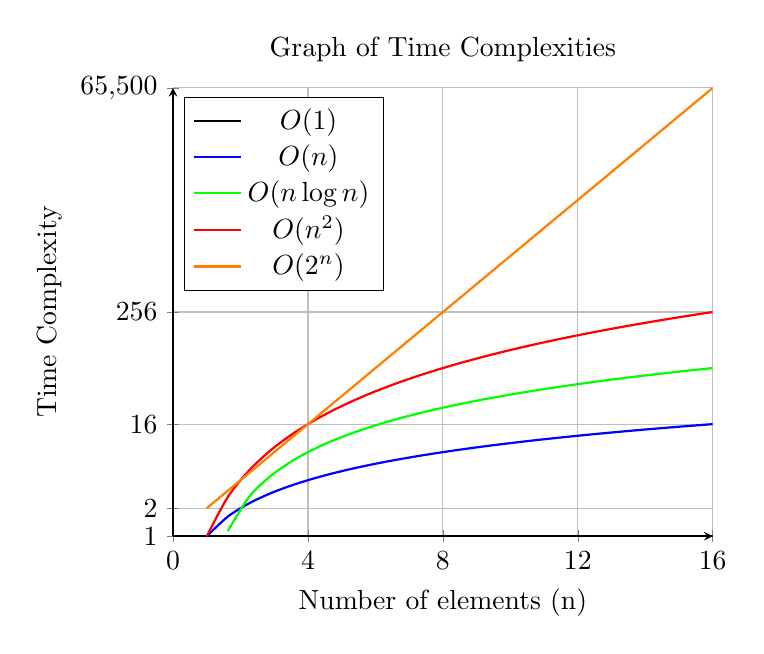
\begin{tikzpicture}
\begin{axis}[
    title={Graph of Time Complexities},
    xlabel={Number of elements (n)},
    ylabel={Time Complexity},
    domain=1:16,
    ymode=log,
    log basis y={2},
    ymin=1,
    ymax=65536,
    xtick={0,4,8,12,16},
    ytick={1,2,16,256,65536},
    log ticks with fixed point,
    axis lines = left,
    grid=both,
    smooth,
    legend style={at={(0.02,0.98)}, anchor=north west}
]
% Constant O(1)
\addplot [
    thick,
    color=black,
    domain=0:16,
] {1};
\addlegendentry{\(O(1)\)}

% Linear O(n)
\addplot [
    thick,
    color=blue,
] {x};
\addlegendentry{\(O(n)\)}

% Linearithmic O(n log n)
\addplot [
    thick,
    color=green,
] {x*log2(x)};
\addlegendentry{\(O(n \log n)\)}

% Quadratic O(n^2)
\addplot [
    thick,
    color=red,
] {x^2};
\addlegendentry{\(O(n^2)\)}

% Exponential O(2^n)
\addplot [
    thick,
    color=orange,
] {2^x};
\addlegendentry{\(O(2^n)\)}
\end{axis}
\end{tikzpicture}

\subsubsection{Big Omega Notation ($\Omega$)}

Big Omega notation describes the lower bound of an algorithm's running time. It provides a guarantee that the algorithm will take at least this much time to complete, even in the best-case scenario.

\[
\Omega(f(n)) = \{ g(n) : \exists c > 0, \exists n_0 \geq 0, \text{ such that } 0 \leq c \cdot f(n) \leq g(n), \forall n \geq n_0 \}
\]

\textbf{Example:} Consider the same algorithm that checks if an array contains a specific element. In the best case, the element might be the first one checked.

\[
T(n) = 1 \implies \Omega(1)
\]

This means that in the best-case scenario, the time complexity is constant, or $\Omega(1)$.


Here are some common Big Omega notations and their typical use cases:
\begin{itemize}
    \item $\Omega(1)$: Constant time – The best-case runtime is constant, regardless of input size.
    \item $\Omega(\log n)$: Logarithmic time – The best-case runtime grows logarithmically with the input size.
    \item $\Omega(n)$: Linear time – The best-case runtime grows linearly with the input size.
    \item $\Omega(n \log n)$: Linearithmic time – The best-case runtime is linearithmic.
    \item $\Omega(n^2)$: Quadratic time – The best-case runtime grows quadratically with the input size.
\end{itemize}

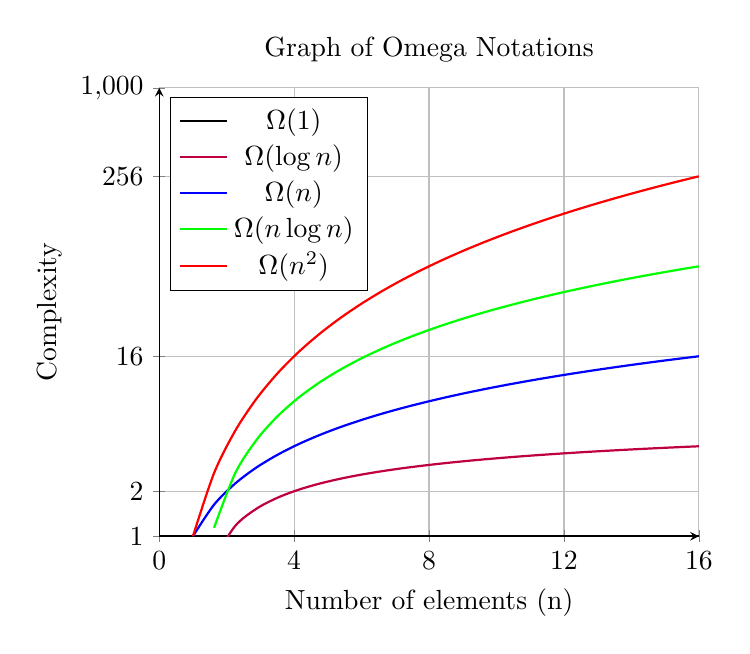
\begin{tikzpicture}
\begin{axis}[
    title={Graph of Omega Notations},
    xlabel={Number of elements (n)},
    ylabel={Complexity},
    domain=1:16,
    ymode=log,
    log basis y={2},
    ymin=1,
    ymax=1000,
    xtick={0,4,8,12,16},
    ytick={1,2,16,256,1000},
    log ticks with fixed point,
    axis lines = left,
    grid=both,
    smooth,
    legend style={at={(0.02,0.98)}, anchor=north west}
]
% Constant Omega(1)
\addplot [
    thick,
    color=black,
    domain=0:16,
] {1};
\addlegendentry{\(\Omega(1)\)}

% Logarithmic Omega(log n)
\addplot [
    thick,
    color=purple,
] {log2(x)};
\addlegendentry{\(\Omega(\log n)\)}

% Linear Omega(n)
\addplot [
    thick,
    color=blue,
] {x};
\addlegendentry{\(\Omega(n)\)}

% Linearithmic Omega(n log n)
\addplot [
    thick,
    color=green,
] {x*log2(x)};
\addlegendentry{\(\Omega(n \log n)\)}

% Quadratic Omega(n^2)
\addplot [
    thick,
    color=red,
] {x^2};
\addlegendentry{\(\Omega(n^2)\)}
\end{axis}
\end{tikzpicture}

\subsubsection{Big Theta Notation ($\Theta$)}

Big Theta notation provides a tight bound on the running time of an algorithm. It means that the algorithm's running time is bounded both above and below by the same function, within constant factors. This gives a more precise characterization of the algorithm's time complexity.

\[
\Theta(f(n)) = \{ g(n) : \exists c_1, c_2 > 0, \exists n_0 \geq 0, \text{ such that } 0 \leq c_1 \cdot f(n) \leq g(n) \leq c_2 \cdot f(n), \forall n \geq n_0 \}
\]

\textbf{Example:} Consider a simple sorting algorithm like insertion sort. In the best case, the array is already sorted, so the time complexity is linear. In the worst case, the array is sorted in reverse order, so the time complexity is quadratic.

\[
T(n) = n^2 \implies \Theta(n^2)
\]

This means that the time complexity is tightly bound and can be expressed as $\Theta(n^2)$.


Here are some common Big Theta notations and their typical use cases:
\begin{itemize}
    \item $\Theta(1)$: Constant time – The runtime is constant, regardless of input size.
    \item $\Theta(\log n)$: Logarithmic time – The runtime grows logarithmically with the input size.
    \item $\Theta(n)$: Linear time – The runtime grows linearly with the input size.
    \item $\Theta(n \log n)$: Linearithmic time – The runtime is linearithmic.
    \item $\Theta(n^2)$: Quadratic time – The runtime grows quadratically with the input size.
\end{itemize}

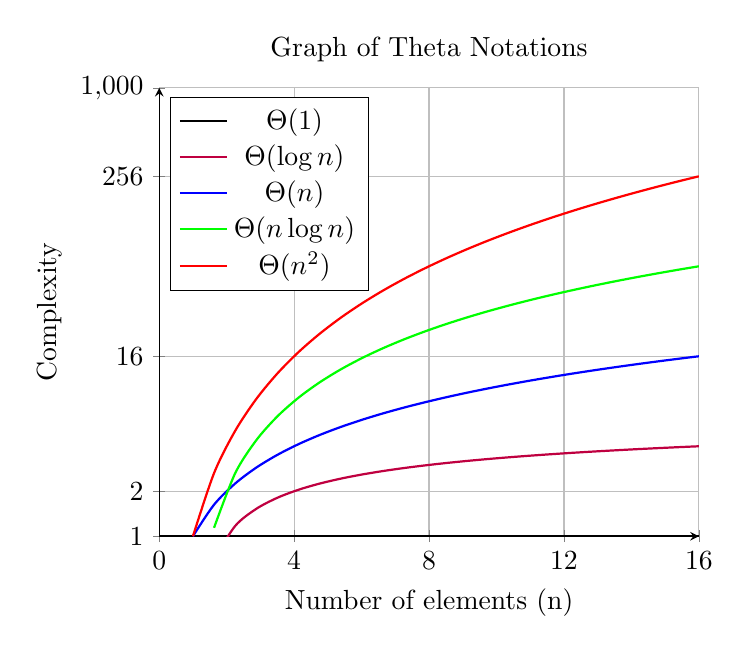
\begin{tikzpicture}
\begin{axis}[
    title={Graph of Theta Notations},
    xlabel={Number of elements (n)},
    ylabel={Complexity},
    domain=1:16,
    ymode=log,
    log basis y={2},
    ymin=1,
    ymax=1000,
    xtick={0,4,8,12,16},
    ytick={1,2,16,256,1000},
    log ticks with fixed point,
    axis lines = left,
    grid=both,
    smooth,
    legend style={at={(0.02,0.98)}, anchor=north west}
]
% Constant Theta(1)
\addplot [
    thick,
    color=black,
    domain=0:16,
] {1};
\addlegendentry{\(\Theta(1)\)}

% Logarithmic Theta(log n)
\addplot [
    thick,
    color=purple,
] {log2(x)};
\addlegendentry{\(\Theta(\log n)\)}

% Linear Theta(n)
\addplot [
    thick,
    color=blue,
] {x};
\addlegendentry{\(\Theta(n)\)}

% Linearithmic Theta(n log n)
\addplot [
    thick,
    color=green,
] {x*log2(x)};
\addlegendentry{\(\Theta(n \log n)\)}

% Quadratic Theta(n^2)
\addplot [
    thick,
    color=red,
] {x^2};
\addlegendentry{\(\Theta(n^2)\)}
\end{axis}
\end{tikzpicture}

\subsection{Asymptotic Tools for Algorithm Analysis}
Here are some tools that help us analyze algorithms more effectively:
\begin{itemize}
    \item \textbf{Recurrence Relations:} These are equations that define sequences recursively. For example, the time complexity of merge sort can be written as:
    \[
    T(n) = 2T\left(\frac{n}{2}\right) + O(n)
    \]
    This means the algorithm divides the problem into two halves, solves each half, and then merges the results, taking linear time to merge.

    \item \textbf{Master Theorem:} This is a handy tool for solving recurrence relations of the form:
    \[
    T(n) = aT\left(\frac{n}{b}\right) + f(n)
    \]
    It gives us different cases to determine the time complexity based on the relationship between $f(n)$ and $n^{\log_b a}$.

    \item \textbf{Amortized Analysis:} This is used when analyzing algorithms that perform a sequence of operations. Instead of looking at the worst-case time for a single operation, we look at the average time over a series of operations. For example, in a dynamic array, resizing happens occasionally, so the average time for insertions is still constant.
\end{itemize}

\subsection{Case Studies in Algorithm Analysis}
Let's look at some common algorithms and their complexities, and understand why they have these time complexities:

\subsubsection{Sorting Algorithms}
\begin{itemize}
    \item \textbf{Quick Sort:}
        \begin{itemize}
            \item \textbf{Average Case:} $O(n \log n)$ – Quick Sort performs well on average because the pivot tends to split the array into two relatively equal halves. This balanced division results in a logarithmic number of recursive levels, each processing $n$ elements.
            \item \textbf{Best Case:} $O(n \log n)$ – The best case occurs when the pivot always divides the array into two equal halves. This results in the most efficient recursive splits.
            \item \textbf{Worst Case:} $O(n^2)$ – The worst case occurs when the pivot is always the smallest or largest element, resulting in highly unbalanced splits. In such cases, the algorithm has to process each element separately, leading to $n$ recursive levels, each with $n$ elements.
        \end{itemize}
        \begin{algorithm}
            \caption{Quick Sort}
            \begin{algorithmic}[1]
                \Procedure{QuickSort}{$A, p, r$}
                    \If{$p < r$}
                        \State $q \gets \textsc{Partition}(A, p, r)$
                        \State \textsc{QuickSort}$(A, p, q-1)$
                        \State \textsc{QuickSort}$(A, q+1, r)$
                    \EndIf
                    \EndProcedure
                \end{algorithmic}
            \end{algorithm}
            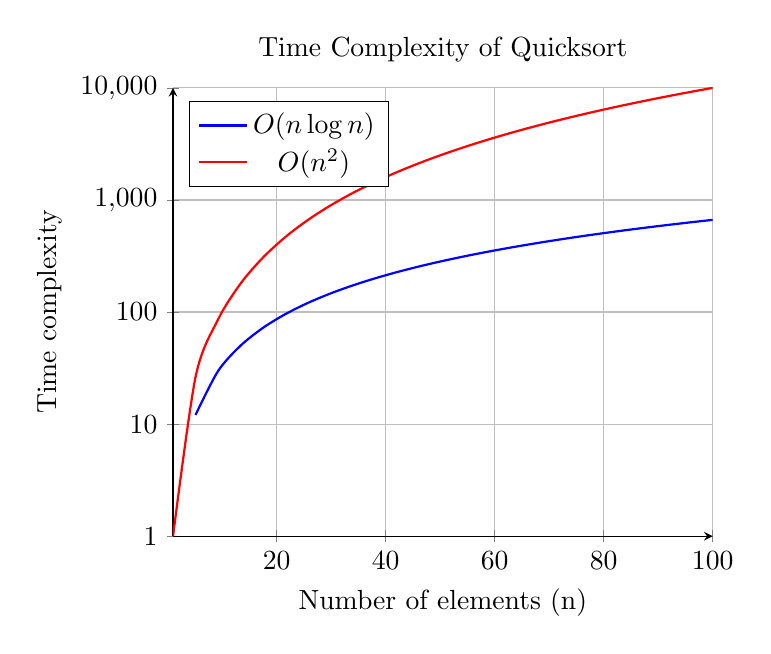
\begin{tikzpicture}
\begin{axis}[
    title={Time Complexity of Quicksort},
    xlabel={Number of elements (n)},
    ylabel={Time complexity},
    domain=1:100,
    legend pos=north west,
    ymode=log,
    log basis y={2},
    ymin=1,
    ymax=10000,
    xtick={0,20,40,60,80,100},
    ytick={1,10,100,1000,10000},
    log ticks with fixed point,
    axis lines = left,
    grid=both,
    smooth
]
% Average and Best Case O(n log n)
\addplot [
    thick,
    color=blue,
] {x*log2(x)};
\addlegendentry{\(O(n \log n)\)}

% Worst Case O(n^2)
\addplot [
    thick,
    color=red,
] {x^2};
\addlegendentry{\(O(n^2)\)}
\end{axis}
\end{tikzpicture}

    \item \textbf{Merge Sort:}
        \begin{itemize}
            \item \textbf{Average Case:} $O(n \log n)$ – Merge Sort consistently divides the array into two equal halves and merges them back together. This balanced division leads to $\log n$ recursive levels, with each level processing $n$ elements.
            \item \textbf{Best Case:} $O(n \log n)$ – Even in the best case, Merge Sort must divide and merge the array, maintaining its $O(n \log n)$ time complexity.
            \item \textbf{Worst Case:} $O(n \log n)$ – The worst case also results in $O(n \log n)$ because the process of dividing and merging is consistent, regardless of the input arrangement.
        \end{itemize}
        \begin{algorithm}
            \caption{Merge Sort}
            \begin{algorithmic}[1]
                \Procedure{MergeSort}{$A, p, r$}
                    \If{$p < r$}
                        \State $q \gets \lfloor \frac{p + r}{2} \rfloor$
                        \State \textsc{MergeSort}$(A, p, q)$
                        \State \textsc{MergeSort}$(A, q+1, r)$
                        \State \textsc{Merge}$(A, p, q, r)$
                    \EndIf
                    \EndProcedure
                \end{algorithmic}
            \end{algorithm}
            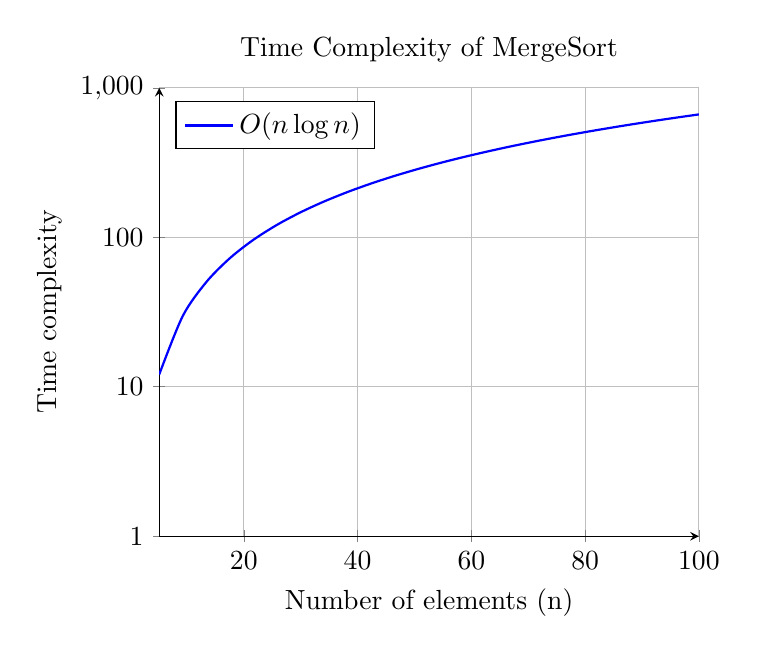
\begin{tikzpicture}
\begin{axis}[
    title={Time Complexity of MergeSort},
    xlabel={Number of elements (n)},
    ylabel={Time complexity},
    domain=1:100,
    legend pos=north west,
    ymode=log,
    log basis y={2},
    ymin=1,
    ymax=1000,
    xtick={0,20,40,60,80,100},
    ytick={1,10,100,1000},
    log ticks with fixed point,
    axis lines = left,
    grid=both,
    smooth
]
% All cases O(n log n)
\addplot [
    thick,
    color=blue,
] {x*log2(x)};
\addlegendentry{\(O(n \log n)\)}
\end{axis}
\end{tikzpicture}

    \item \textbf{Bubble Sort:}
        \begin{itemize}
            \item \textbf{Average Case:} $O(n^2)$ – On average, Bubble Sort needs to compare and swap elements multiple times, resulting in quadratic time complexity.
            \item \textbf{Best Case:} $O(n)$ – In the best case, the array is already sorted, so Bubble Sort only needs one pass through the array to confirm it's sorted. This results in linear time complexity.
            \item \textbf{Worst Case:} $O(n^2)$ – In the worst case, the array is sorted in reverse order. Bubble Sort needs to perform $n$ passes, with each pass involving $n-1$ comparisons and swaps, leading to quadratic time complexity.
        \end{itemize}
        \begin{algorithm}
            \caption{Bubble Sort}
            \begin{algorithmic}[1]
                \Procedure{BubbleSort}{$A, n$}
                    \For{$i \gets 1$ to $n-1$}
                        \For{$j \gets 0$ to $n-i-1$}
                            \If{$A[j] > A[j+1]$}
                                \State \text{Swap } $A[j]$ and $A[j+1]$
                            \EndIf
                        \EndFor
                    \EndFor
                    \EndProcedure
                \end{algorithmic}
            \end{algorithm}
            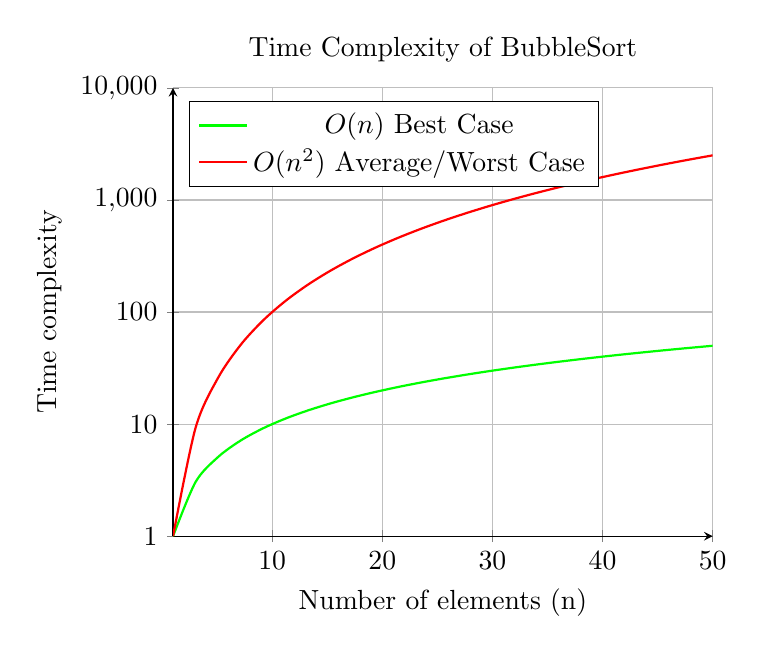
\begin{tikzpicture}
\begin{axis}[
    title={Time Complexity of BubbleSort},
    xlabel={Number of elements (n)},
    ylabel={Time complexity},
    domain=1:50,
    legend pos=north west,
    ymode=log,
    log basis y={2},
    ymin=1,
    ymax=10000,
    xtick={0,10,20,30,40,50},
    ytick={1,10,100,1000,10000},
    log ticks with fixed point,
    axis lines = left,
    grid=both,
    smooth
]
% Best Case O(n)
\addplot [
    thick,
    color=green,
] {x};
\addlegendentry{\(O(n)\) Best Case}

% Average and Worst Case O(n^2)
\addplot [
    thick,
    color=red,
] {x^2};
\addlegendentry{\(O(n^2)\) Average/Worst Case}
\end{axis}
\end{tikzpicture}
\end{itemize}

\subsubsection{Search Algorithms}
\begin{itemize}
    \item \textbf{Linear Search:}
        \begin{itemize}
            \item \textbf{Average Case:} $O(n)$ – On average, Linear Search needs to check half of the elements in the array, resulting in linear time complexity.
            \item \textbf{Best Case:} $O(1)$ – In the best case, the target element is the first one in the array, so the search completes in constant time.
            \item \textbf{Worst Case:} $O(n)$ – In the worst case, the target element is the last one in the array or not present at all, requiring a check of all $n$ elements.
        \end{itemize}
        \begin{algorithm}
            \caption{Linear Search}
            \begin{algorithmic}[1]
                \Procedure{LinearSearch}{$A, n, x$}
                    \For{$i \gets 0$ to $n-1$}
                        \If{$A[i] = x$}
                            \State \Return $i$
                        \EndIf
                    \EndFor
                    \State \Return -1
                    \EndProcedure
                \end{algorithmic}
            \end{algorithm}
            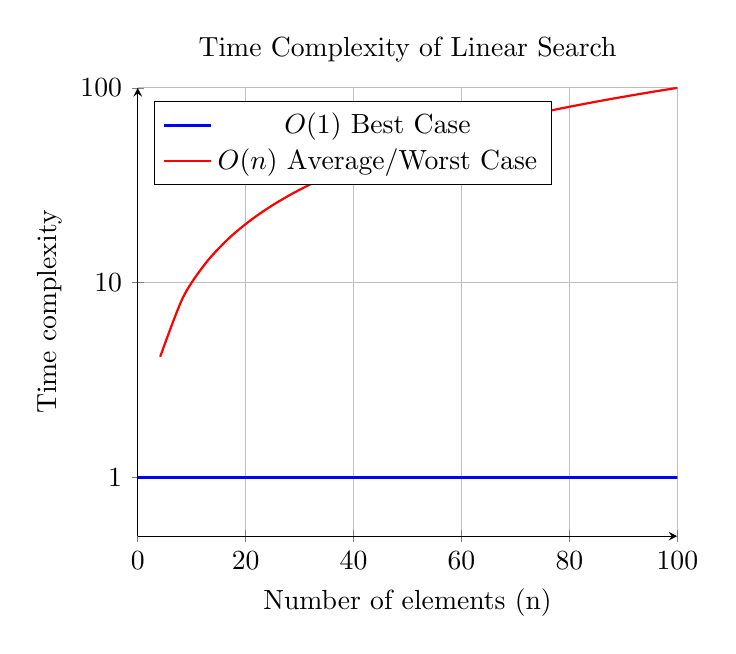
\begin{tikzpicture}
\begin{axis}[
    title={Time Complexity of Linear Search},
    xlabel={Number of elements (n)},
    ylabel={Time complexity},
    domain=0:100,
    legend pos=north west,
    ymode=log,
    log basis y={2},
    ymin=0.5,
    ymax=100,
    xtick={0,20,40,60,80,100},
    ytick={1,10,100},
    log ticks with fixed point,
    axis lines = left,
    grid=both,
    smooth
]
% Best Case O(1)
\addplot [
    thick,
    color=blue,
    domain=0:100,
] {1};
\addlegendentry{\(O(1)\) Best Case}

% Average and Worst Case O(n)
\addplot [
    thick,
    color=red,
] {x};
\addlegendentry{\(O(n)\) Average/Worst Case}
\end{axis}
\end{tikzpicture}

    \item \textbf{Binary Search:}
        \begin{itemize}
            \item \textbf{Average Case:} $O(\log n)$ – On average, Binary Search reduces the search space by half with each step, resulting in logarithmic time complexity.
            \item \textbf{Best Case:} $O(1)$ – In the best case, the target element is the middle element of the array, found in the first comparison.
            \item \textbf{Worst Case:} $O(\log n)$ – In the worst case, the search space is reduced to a single element, requiring $\log n$ comparisons.
        \end{itemize}
        \begin{algorithm}
            \caption{Binary Search}
            \begin{algorithmic}[1]
                \Procedure{BinarySearch}{$A, p, r, x$}
                    \If{$p \leq r$}
                        \State $q \gets \lfloor \frac{p + r}{2} \rfloor$
                        \If{$A[q] = x$}
                            \State \Return $q$
                        \ElsIf{$A[q] > x$}
                            \State \Return \textsc{BinarySearch}$(A, p, q-1, x)$
                        \Else
                            \State \Return \textsc{BinarySearch}$(A, q+1, r, x)$
                        \EndIf
                    \Else
                        \State \Return -1
                    \EndIf
                    \EndProcedure
                \end{algorithmic}
            \end{algorithm}
            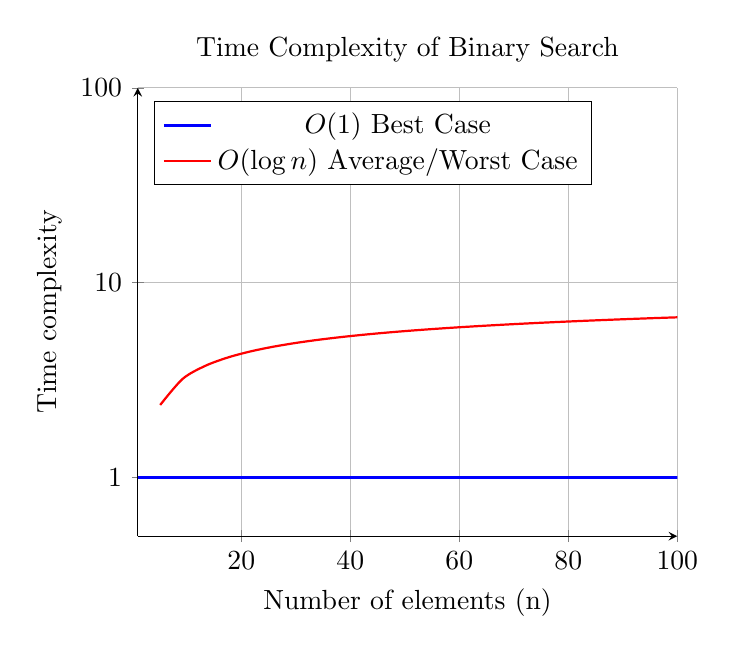
\begin{tikzpicture}
\begin{axis}[
    title={Time Complexity of Binary Search},
    xlabel={Number of elements (n)},
    ylabel={Time complexity},
    domain=1:100,
    legend pos=north west,
    ymode=log,
    log basis y={2},
    ymin=0.5,
    ymax=100,
    xtick={0,20,40,60,80,100},
    ytick={1,10,100},
    log ticks with fixed point,
    axis lines = left,
    grid=both,
    smooth
]
% Best Case O(1)
\addplot [
    thick,
    color=blue,
    domain=1:100,
] {1};
\addlegendentry{\(O(1)\) Best Case}

% Average and Worst Case O(log n)
\addplot [
    thick,
    color=red,
] {log2(x)};
\addlegendentry{\(O(\log n)\) Average/Worst Case}
\end{axis}
\end{tikzpicture}
\end{itemize}

\subsubsection{Graph Algorithms}
\begin{itemize}
    \item \textbf{Dijkstra’s Algorithm:}
        \begin{itemize}
            \item \textbf{Average Case:} $O((V + E) \log V)$ – Using a priority queue with an adjacency list, the algorithm efficiently finds the shortest path from a source to all other vertices.
            \item \textbf{Best Case:} $O((V + E) \log V)$ – Even in the best case, the algorithm still needs to explore all vertices and edges, maintaining its time complexity.
            \item \textbf{Worst Case:} $O(V^2 + E)$ – With an adjacency matrix, the algorithm needs to check each vertex pair, leading to higher time complexity.
        \end{itemize}
        \begin{algorithm}
            \caption{Dijkstra's Algorithm}
            \begin{algorithmic}[1]
                \Procedure{Dijkstra}{$G, w, s$}
                    \For{each vertex $v \in G$}
                        \State $d[v] \gets \infty$
                        \State $p[v] \gets \text{NIL}$
                    \EndFor
                    \State $d[s] \gets 0$
                    \State $Q \gets \text{priority queue containing all vertices}$
                    \While{$Q \neq \emptyset$}
                        \State $u \gets \text{Extract-Min}(Q)$
                        \For{each vertex $v \in \text{Adj}[u]$}
                            \If{$d[v] > d[u] + w(u, v)$}
                                \State $d[v] \gets d[u] + w(u, v)$
                                \State $p[v] \gets u$
                            \EndIf
                        \EndFor
                    \EndWhile
                    \EndProcedure
                \end{algorithmic}
            \end{algorithm}
            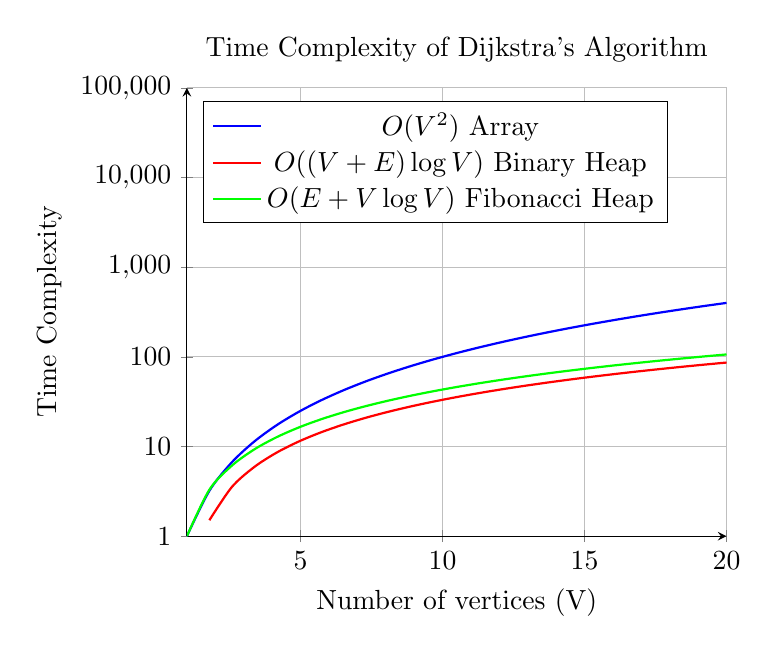
\begin{tikzpicture}
\begin{axis}[
    title={Time Complexity of Dijkstra's Algorithm},
    xlabel={Number of vertices (V)},
    ylabel={Time Complexity},
    domain=1:20,
    legend pos=north west,
    ymode=log,
    log basis y={2},
    ymin=1,
    ymax=100000,
    xtick={0,5,10,15,20},
    ytick={1,10,100,1000,10000,100000},
    log ticks with fixed point,
    axis lines = left,
    grid=both,
    smooth
]
% Using an array O(V^2)
\addplot [
    thick,
    color=blue,
] {x^2};
\addlegendentry{\(O(V^2)\) Array}

% Using binary heap O((V + E) log V)
\addplot [
    thick,
    color=red,
] {x*log2(x)};
\addlegendentry{\(O((V+E) \log V)\) Binary Heap}

% Using Fibonacci heap O(E + V log V)
\addplot [
    thick,
    color=green,
] {x*log2(x) + x};
\addlegendentry{\(O(E + V \log V)\) Fibonacci Heap}
\end{axis}
\end{tikzpicture}

    \item \textbf{Bellman-Ford Algorithm:}
        \begin{itemize}
            \item \textbf{Average Case:} $O(VE)$ – The algorithm checks all edges for each vertex, ensuring the shortest path even with negative weights.
            \item \textbf{Best Case:} $O(VE)$ – The best case also requires checking all edges for each vertex to handle negative weights.
            \item \textbf{Worst Case:} $O(VE)$ – The worst case involves checking all edges for each vertex, leading to higher time complexity.
        \end{itemize}
        \begin{algorithm}
            \caption{Bellman-Ford Algorithm}
            \begin{algorithmic}[1]
                \Procedure{BellmanFord}{$G, w, s$}
                    \For{each vertex $v \in G$}
                        \State $d[v] \gets \infty$
                        \State $p[v] \gets \text{NIL}$
                    \EndFor
                    \State $d[s] \gets 0$
                    \For{$i \gets 1$ to $|V| - 1$}
                        \For{each edge $(u, v) \in E$}
                            \If{$d[v] > d[u] + w(u, v)$}
                                \State $d[v] \gets d[u] + w(u, v)$
                                \State $p[v] \gets u$
                            \EndIf
                        \EndFor
                    \EndFor
                    \For{each edge $(u, v) \in E$}
                        \If{$d[v] > d[u] + w(u, v)$}
                            \State \Return \text{False} \Comment{Negative weight cycle}
                        \EndIf
                    \EndFor
                    \State \Return \text{True}
                    \EndProcedure
                \end{algorithmic}
            \end{algorithm}
            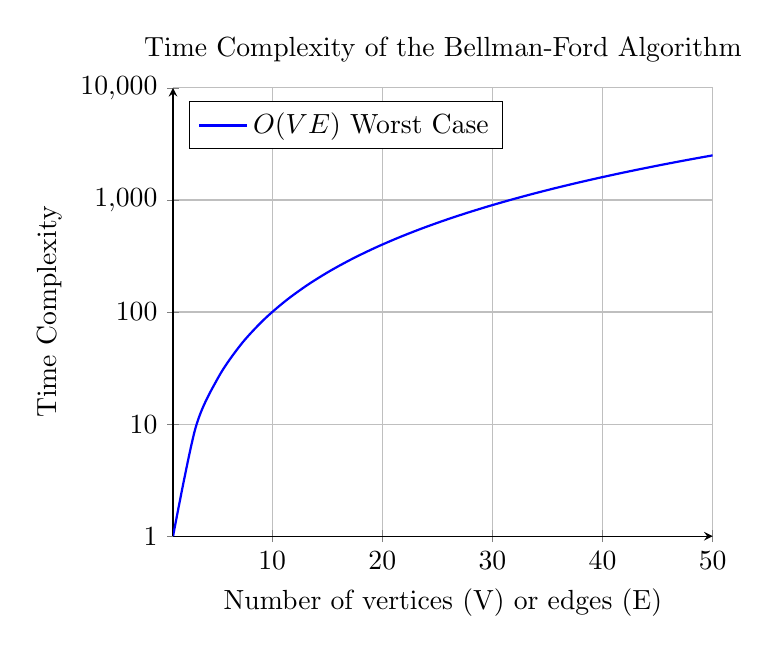
\begin{tikzpicture}
\begin{axis}[
    title={Time Complexity of the Bellman-Ford Algorithm},
    xlabel={Number of vertices (V) or edges (E)},
    ylabel={Time Complexity},
    domain=1:50,
    legend pos=north west,
    ymode=log,
    log basis y={2},
    ymin=1,
    ymax=10000,
    xtick={0,10,20,30,40,50},
    ytick={1,10,100,1000,10000},
    log ticks with fixed point,
    axis lines = left,
    grid=both,
    smooth
]
% Worst Case O(VE)
\addplot [
    thick,
    color=blue,
] {x*x};
\addlegendentry{\(O(VE)\) Worst Case}
\end{axis}
\end{tikzpicture}
\end{itemize}


\subsection{Advanced Topics}
Let's dive into some more advanced concepts:
\begin{itemize}
    \item \textbf{Randomized Algorithms:} These use random choices to make decisions, often leading to simpler and faster algorithms. For example, Randomized QuickSort randomly selects a pivot to avoid the worst-case scenario.
    \begin{algorithm}
        \caption{Randomized QuickSort}
        \begin{algorithmic}[1]
            \Procedure{Randomized-Partition}{$A, p, r$}
                \State $i \gets \text{Random}(p, r)$
                \State \text{Swap } $A[r]$ and $A[i]$
                \State \Return \textsc{Partition}$(A, p, r)$
            \EndProcedure
        \end{algorithmic}
    \end{algorithm}


    \item \textbf{Parallel Algorithms:} These break down tasks into sub-tasks that can be executed simultaneously. For example, Parallel Merge Sort splits the array and sorts the halves concurrently.
    \begin{algorithm}
        \caption{Parallel Merge Sort}
        \begin{algorithmic}[1]
            \Procedure{Parallel-Merge-Sort}{$A, p, r$}
                \If{$p < r$}
                    \State $q \gets \lfloor \frac{p + r}{2} \rfloor$
                    \State \text{Fork: \textsc{Parallel-Merge-Sort}}$(A, p, q)$
                    \State \text{Fork: \textsc{Parallel-Merge-Sort}}$(A, q+1, r)$
                    \State \text{Join: \textsc{Merge}}$(A, p, q, r)$
                \EndIf
            \EndProcedure
        \end{algorithmic}
    \end{algorithm}
  

    \item \textbf{Approximation Algorithms:} These algorithms provide solutions that are close to the optimal solution. For example, the Traveling Salesman Problem (TSP) can be solved using a 2-approximation algorithm, where the solution is at most twice the optimal solution.
\end{itemize}

\subsection{Conclusion}
Understanding algorithm analysis is like having a map to navigate the world of algorithms. It helps you choose the best tools for the job and optimize your solutions effectively. 



\chapter{Graph Algorithms}
\section{Introduction to Graph Theory}

Graph theory is a vibrant area of mathematics that studies graphs—simple structures that model relationships between pairs of objects. These objects are represented as vertices (or nodes), and the connections between them are edges (or links). Whether in computer science, biology, or social science, graph theory plays a crucial role by providing a framework to solve problems involving connected data.


Graphs come in several flavors:
- \textbf{Undirected graphs} where edges have no direction.
- \textbf{Directed graphs} where edges point from one vertex to another.
- \textbf{Weighted graphs} where edges carry weights, representing costs, lengths, or capacities.

\textbf{Exploring Graph Theory}

Studying graph theory involves:
- Examining the properties of graphs to understand their structure.
- Developing algorithms to tackle problems like finding the shortest path between nodes or determining the most efficient way to connect various points.
- Applying graph theory concepts to practical scenarios across different fields, showing how these abstract ideas help solve real-world problems.

In summary, graph theory not only enriches our mathematical understanding but also enhances our ability to address complex issues in various scientific and practical domains.



\subsection{Definition of Graphs}

At its core, a graph \( G = (V, E) \) in graph theory is made up of vertices \( V \) and edges \( E \), where each edge connects a pair of vertices. This setup is used to model the relationships between different entities. Depending on the nature of these relationships, edges can be directed or undirected, and the graph can either carry weights on its edges or not.

\subsection{Types of Graphs}

Graph theory classifies graphs into several types based on their properties and the nature of the connections between their nodes. Understanding these types helps in applying the right kind of graph to solve specific problems effectively.

1. \textbf{Directed Graphs}: In these graphs, edges point from one vertex to another, establishing a clear direction from the source to the destination. This structure is useful in scenarios like city traffic flows where roads have definite directions.

2. \textbf{Undirected Graphs}: These graphs feature edges that don’t have a directed flow, meaning the relationship between the connected vertices is bidirectional. They are ideal for modeling undirected connections like telephone lines between cities.

3. \textbf{Weighted Graphs}: Here, edges carry weights, which could be costs, distances, or any other measurable attribute. This type is particularly useful in route planning and network optimization, where the cost of traversing edges varies significantly.

4. \textbf{Connected Graphs}: Every pair of vertices in a connected graph is linked by a path. This type ensures there are no isolated vertices or disjoint subgraphs, which is crucial for network design to ensure every node is reachable.

5. \textbf{Complete Graphs}: These graphs feature an edge between every pair of vertices. They represent a fully connected network, often used in problems requiring exhaustive interconnection, like circuit design or social network analysis.

Each type of graph has its specific use cases, and choosing the correct type is key to efficiently solving complex graph-based problems.


\subsubsection{Directed vs. Undirected Graphs}
In graph theory, graphs can be categorized into two main types based on the nature of their edges - directed graphs and undirected graphs.
\FloatBarrier
\textbf{Directed Graphs}:
\FloatBarrier
In a directed graph, the edges have a direction associated with them. This means that the relationship between any two nodes is asymmetric. If there is an edge from node A to node B, it does not imply the existence of an edge from node B to node A.
\FloatBarrier
\paragraph{Example: Depth-First Search (DFS) on a Directed Graph}
\FloatBarrier
\begin{algorithm}
\caption{Depth-First Search (DFS) on a Directed Graph}
\begin{algorithmic}[1]
\Function{DFS}{$G, v$}
    \State Mark vertex $v$ as visited
    \For{each adjacent vertex $u$ of $v$}
        \If{$u$ is not visited}
            \State \textsc{DFS}($G, u$)
        \EndIf
    \EndFor
\EndFunction
\end{algorithmic}
\end{algorithm}

\textbf{Algorithm Explanation:}

The Depth-First Search (DFS) algorithm is used to traverse or search a graph. In the case of a directed graph, DFS starts from a given vertex $v$ and explores as far as possible along each branch before backtracking.

\textbf{Mathematical Detail:}

Let $G(V, E)$ be a directed graph with vertices $V$ and edges $E$. The DFS algorithm visits each vertex in $G$ exactly once, making it $O(|V|)$ in time complexity, where $|V|$ is the number of vertices in $G$. 

Suppose the DFS algorithm starts from vertex $v_0$. It explores all vertices reachable from $v_0$ in a depth-first manner. Let $n$ be the number of vertices reachable from $v_0$. The DFS algorithm has a space complexity of $O(n)$ because it stores information about the vertices it has visited, typically using a stack or recursion.

The DFS algorithm can be used for various purposes in directed graphs, such as detecting cycles, finding strongly connected components, and topological sorting.
\FloatBarrier
\textbf{Undirected Graphs}:
\FloatBarrier
In an undirected graph, the edges do not have any direction associated with them. This means that the relationship between any two nodes is symmetrical. If there is an edge between node A and node B, it implies the existence of an edge between node B and node A.
\FloatBarrier
\paragraph{Example: Depth-First Search (DFS) on a Undirected Graph}
\FloatBarrier
\begin{algorithm}
\caption{Depth First Search on an Undirected Graph}
\begin{algorithmic}[1]
\Procedure{DFS}{$G$, $v$}
    \State \textbf{Input:} Graph $G$ as an adjacency list, start vertex $v$
    \State \textbf{Output:} All vertices reachable from $v$ are marked as visited
    \State Create a set $Visited$ to track visited nodes
    \State Call \Call{DFS-Visit}{$v$, $Visited$}
\EndProcedure
\Statex
\Procedure{DFS-Visit}{$v$, $Visited$}
    \State Mark $v$ as visited: $Visited$.add($v$)
    \State Output $v$ \Comment{Process the current node}
    \For{each neighbor $u$ of $v$ in $G[v]$}
        \If{$u$ not in $Visited$}
            \State Call \Call{DFS-Visit}{$u$, $Visited$}
        \EndIf
    \EndFor
\EndProcedure
\end{algorithmic}
\end{algorithm}
\FloatBarrier
\subsubsection{Weighted vs. Unweighted Graphs}

In graph theory, graphs are generally divided into two categories based on edge characteristics: weighted and unweighted.

\textbf{Unweighted Graphs}: These graphs treat all edges equally, as each edge has the same weight or no weight at all. Unweighted graphs are ideal for situations where only the connection matters, not the strength or capacity of that connection. They simplify modeling relationships where every link is of equal value, such as friendships in a social network where the presence of a connection is more important than its intensity.

\textbf{Weighted Graphs}: In contrast, weighted graphs assign a numerical weight to each edge, which can represent distance, cost, time, or other metrics. This feature makes weighted graphs essential for accurately modeling real-world problems where not all connections are created equal. For instance, in a road network, edges can represent the distance or travel time between locations, affecting route planning.

\textbf{Implications for Algorithms}: The type of graph impacts how algorithms perform. For example, finding the shortest path in a network is straightforward in unweighted graphs where each step counts the same. However, in weighted graphs, algorithms like Dijkstra's need to consider the weights to optimize the path based on actual travel costs or distances.

Understanding whether to use a weighted or unweighted graph depends on the specific requirements of the application and the nature of the entities being modeled. This decision is crucial as it influences both the complexity of the problem and the choice of algorithms for processing the graph.


\subsubsection*{Algorithmic Example: Dijkstra's Algorithm}

Dijkstra's algorithm is a widely-used algorithm for finding the shortest path between nodes in a weighted graph. Given a weighted graph, the algorithm calculates the shortest path from a source node to all other nodes in the graph.
\FloatBarrier
Let's consider a weighted graph represented by an adjacency matrix:
\FloatBarrier
\[ \begin{pmatrix}
0 & 4 & 0 & 0 & 0 \\
0 & 0 & 8 & 0 & 0 \\
0 & 0 & 0 & 7 & 0 \\
0 & 0 & 0 & 0 & 5 \\
0 & 0 & 0 & 0 & 0
\end{pmatrix} \]
\FloatBarrier
The Python implementation of Dijkstra's algorithm for finding the shortest path from a given source node to all other nodes in the graph can be represented as follows:
\FloatBarrier
\begin{algorithm}
\caption{Dijkstra's Algorithm}
\begin{algorithmic}[1]
\Procedure{Dijkstra}{graph, source}
\State $distances \gets$ Array filled with $\infty$ of size $|V|$ \Comment{Initialize distances array}
\State $distances[source] \gets 0$ \Comment{Distance from source to itself is 0}
\State $visited \gets$ Empty set \Comment{Initialize set of visited nodes}

\While{There are unvisited nodes}
    \State $v \gets$ Node with the minimum distance in $distances$ \Comment{Select unvisited node}
    \State $visited$.add($v$) \Comment{Mark node as visited}
    
    \For{each neighbor $u$ of $v$}
        \State $alt \gets$ distance[$v$] + weight of edge $(v, u)$
        \If{$alt < distances[u]$}
            \State $distances[u] \gets alt$ \Comment{Update distance if shorter path found}
        \EndIf
    \EndFor
\EndWhile

\State \textbf{return} $distances$
\EndProcedure
\end{algorithmic}
\end{algorithm}
\FloatBarrier
This algorithm calculates the shortest path from the given source node to all other nodes in the graph. The resulting distances array will contain the shortest path distances from the source node to each node in the graph.

\subsection{Bipartiteness in Graphs}

\textbf{Understanding and Testing for Bipartiteness}

A graph is bipartite if its vertices can be divided into two disjoint sets, $U$ and $V$, such that every edge connects a vertex in $U$ to a vertex in $V$. This means there are no edges between vertices within the same set. Mathematically, a graph $G = (V, E)$ is bipartite if $V$ can be partitioned into $U$ and $V$ such that for every edge $(u, v) \in E$, either $u \in U$ and $v \in V$ or $u \in V$ and $v \in U$.

To test for bipartiteness, we can use a BFS or DFS algorithm to attempt to color the graph using two colors. If we can successfully color the graph without two adjacent vertices sharing the same color, the graph is bipartite. Otherwise, it is not.

\begin{algorithm}[H]
\caption{Bipartiteness Test using BFS}
\begin{algorithmic}[1]
\Procedure{IsBipartite}{$G$}
    \State Let $color$ be an array of size $|V|$ with all values initialized to $-1$
    \For{each vertex $u \in V$}
        \If{$color[u] = -1$}
            \State Let $queue$ be an empty queue
            \State Enqueue $u$ and set $color[u] = 0$
            \While{$queue$ is not empty}
                \State Dequeue $v$
                \For{each neighbor $w$ of $v$}
                    \If{$color[w] = -1$}
                        \State Set $color[w] = 1 - color[v]$
                        \State Enqueue $w$
                    \ElsIf{$color[w] = color[v]$}
                        \State \Return False
                    \EndIf
                \EndFor
            \EndWhile
        \EndIf
    \EndFor
    \State \Return True
\EndProcedure
\end{algorithmic}
\end{algorithm}

\textbf{Applications of Bipartite Graphs}

Bipartite graphs have various practical applications:

\begin{itemize}
    \item \textbf{Matching Problems:} In job assignment problems where workers need to be matched to tasks, bipartite graphs can represent feasible assignments.
    \item \textbf{Network Flow:} In network flow problems, bipartite graphs help in modeling flows between two sets of nodes, such as sources and sinks.
    \item \textbf{Scheduling:} In scheduling tasks with specific constraints, bipartite graphs can model the relationship between tasks and resources.
    \item \textbf{Recommendation Systems:} Bipartite graphs are used in recommendation systems to model relationships between users and items, facilitating collaborative filtering algorithms.
\end{itemize}


\subsection{Representations of Graphs}

In computer science, how we represent graphs in data structures is crucial for efficient storage and manipulation. Two of the most common graph representations are the adjacency matrix and the adjacency list.

\textbf{Adjacency Matrix}: This representation uses a 2D array where both rows and columns correspond to vertices in the graph. An entry at \(A[i][j]\) indicates the presence of an edge between vertex \(i\) and vertex \(j\). If an edge exists, the entry is set to 1 or to the weight of the edge in a weighted graph. If no edge exists, it's set to 0, or \(\infty\) in weighted graphs to denote an absence of direct paths.

\textbf{Adjacency List}: Alternatively, an adjacency list uses a list of lists. Each list corresponds to a vertex and contains the vertices that are directly connected to it. This method is space-efficient, especially for sparse graphs, as it only stores information about existing edges.

Each representation has its advantages depending on the operations required and the density of the graph. The adjacency matrix makes it quick and easy to check if an edge exists between any two vertices but can be space-intensive for large sparse graphs. On the other hand, adjacency lists are more space-efficient for sparse graphs but can require more time to check for the existence of a specific edge. Choosing the right representation is key to optimizing the performance of graph algorithms.


Algorithm Example: Finding the degree of a vertex in a graph using an adjacency list representation.
\FloatBarrier
\begin{algorithm}
\caption{Find Degree of a Vertex using Adjacency List}
\begin{algorithmic}
\State \textbf{Input:} Graph $G$ represented as an adjacency list, Vertex $v$
\State \textbf{Output:} Degree of Vertex $v$

\Function{Degree}{$G, v$}
    \State $degree \gets |G[v]|$ \Comment{Get the length of the adjacency list for vertex $v$}
    \State \textbf{return} $degree$
\EndFunction
\end{algorithmic}
\end{algorithm}
\FloatBarrier

These representations have their own advantages and are selected based on the operations expected to be performed on the graph data structure. The choice of representation can significantly impact the efficiency of algorithms that work on graphs.

\subsubsection{Adjacency Matrix}

An adjacency matrix is a way to represent a graph as a square matrix where the rows and columns are indexed by vertices. The entry at row $i$ and column $j$ represents whether there is an edge from vertex $i$ to vertex $j$. If the graph is unweighted, the entry will be either 0 (no edge) or 1 (edge exists). In the case of a weighted graph, the entry can hold the weight of the edge.
\FloatBarrier
Algorithmic Example:
\FloatBarrier
Let's consider a simple undirected graph with 4 vertices and the following edges: (1, 2), (2, 3), (3, 4), (4, 1).
\FloatBarrier
\begin{figure}[h]
\centering
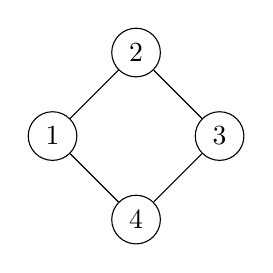
\begin{tikzpicture}[node distance={15mm}, main/.style = {draw, circle}] 
\node[main] (1) {$1$}; 
\node[main] (2) [above right of=1] {$2$}; 
\node[main] (3) [below right of=2] {$3$}; 
\node[main] (4) [below right of=1] {$4$}; 

\draw (1) -- (2);
\draw (2) -- (3);
\draw (3) -- (4);
\draw (4) -- (1);
\end{tikzpicture}
\caption{Undirected Graph Example}
\end{figure}
\FloatBarrier
The adjacency matrix for this graph would look like:
\FloatBarrier
\[
\begin{bmatrix}
0 & 1 & 0 & 1 \\
1 & 0 & 1 & 0 \\
0 & 1 & 0 & 1 \\
1 & 0 & 1 & 0 \\
\end{bmatrix}
\]
\FloatBarrier
This matrix reflects the connections between vertices in the graph.
\FloatBarrier
Equivalent Python code for constructing the adjacency matrix:
\FloatBarrier
\begin{lstlisting}
def adjacency_matrix(graph):
    n = len(graph)
    adj_matrix = [[0] * n for _ in range(n)]
    
    for edge in graph:
        node1, node2 = edge
        adj_matrix[node1][node2] = 1
        adj_matrix[node2][node1] = 1
    
    return adj_matrix

graph = [(0, 1), (1, 2), (2, 3), (3, 0)]
adj_matrix = adjacency_matrix(graph)
print(adj_matrix)
\end{lstlisting}
\FloatBarrier
This Python function takes a graph as an input (list of edges) and constructs the corresponding adjacency matrix. In the example provided, the graph has the edges (0, 1), (1, 2), (2, 3), and (3, 0). The resulting adjacency matrix is printed out.
Sure, I can help you with that. Here is an expanded explanation of the \texttt{Adjacency List} approach in LaTeX format along with an algorithmic example and its equivalent Python code.

\subsubsection{Adjacency List}

In the adjacency list representation of a graph, each vertex in the graph is associated with a list of its neighboring vertices. This representation is quite efficient for sparse graphs where the number of edges is much smaller compared to the number of possible edges. It requires less memory storage compared to the adjacency matrix representation, especially when the graph is sparse.

When using an adjacency list to represent a graph, we can easily find all the neighbors of a specific vertex by looking at its associated list. This makes it efficient for algorithms like traversals and shortest-path algorithms.
\FloatBarrier
Algorithm:
\FloatBarrier
Let \( G(V, E) \) be a graph with vertices \( V = \{v_1, v_2, ..., v_n\} \) and edges \( E = \{e_1, e_2, ..., e_m\} \). The adjacency list representation of \( G \) is a set of \( n \) lists, one for each vertex \( v_i \), where each list contains the vertices adjacent to \( v_i \).
\FloatBarrier
\textbf{Example:}
\FloatBarrier
Let's consider a simple undirected graph with 4 vertices and 4 edges:
\FloatBarrier
\[ V = \{v_1, v_2, v_3, v_4\} \]
\[ E = \{(v_1, v_2), (v_2, v_3), (v_3, v_4), (v_1, v_4)\} \]
\FloatBarrier
The adjacency list for this graph would be:
\FloatBarrier
\[ v_1: [v_2, v_4] \]
\[ v_2: [v_1, v_3] \]
\[ v_3: [v_2, v_4] \]
\[ v_4: [v_1, v_3] \]
\FloatBarrier
\textbf{Algorithmic example:}
\begin{algorithm}
\caption{Create Adjacency List of a Graph}
\begin{algorithmic}
\State Let $adjList$ be an empty dictionary
\For{each edge $(u, v)$ in $E$}
    \State Add $v$ to $adjList[u]$
    \State Add $u$ to $adjList[v]$
\EndFor
\end{algorithmic}
\end{algorithm}
\FloatBarrier


\section{Graph Traversal Techniques}
Graph traversal is the process of visiting all the nodes in a graph in a systematic way. There are several techniques for graph traversal, some of the common ones include:
\begin{itemize}
    \item Breadth-first Search (BFS): In BFS, we visit all the neighbors of a node before moving on to the next level of nodes.
    \item Depth-first Search (DFS): In DFS, we explore as far as possible along each branch before backtracking.
\end{itemize}

\subsection{Breadth-First Search (BFS)}
Breadth-First Search (BFS) is an algorithm used for traversing or searching tree or graph data structures. It starts at the tree root or any arbitrary node of a graph, and explores all of the neighbor nodes at the present depth prior to moving on to the nodes at the next depth level. This ensures that the algorithm traverses the graph in layers. BFS is often used to find the shortest path in unweighted graphs.

\subsubsection{Algorithm Overview}


\FloatBarrier
\begin{algorithm}
\caption{Breadth-First Search (BFS)}
\begin{algorithmic}
\State $Q \gets$ Queue data structure
\State $visited \gets$ Set to keep track of visited nodes
\State $Q.push(start)$ \Comment{Start with the initial node}
\State $visited.add(start)$
\While{$Q$ is not empty}
    \State $current \gets Q.pop()$
    \For{each neighbor $n$ of $current$}
        \If{$n$ is not in $visited$}
            \State $Q.push(n)$
            \State $visited.add(n)$
        \EndIf
    \EndFor
\EndWhile
\end{algorithmic}
\end{algorithm}
\FloatBarrier


\subsubsection{Applications and Examples}

The Breadth First Search (BFS) algorithm is a cornerstone of graph traversal techniques, widely appreciated for its simplicity and effectiveness across various fields. Here are some key applications:

\textbf{Shortest Path and Distance Calculation}
Primarily, BFS is used to identify the shortest path and calculate distances in unweighted graphs. It explores the graph layer by layer from the source node, ensuring that the shortest paths are identified efficiently.

\textbf{Example:} In navigation systems, BFS helps calculate the most direct route between locations, considering each junction or road one by one from the starting point.

\textbf{Connected Components}
BFS is also instrumental in detecting connected components in undirected graphs. By launching BFS from various nodes, it's possible to group nodes into clusters based on connectivity.

\textbf{Example:} In social network analysis, BFS can determine groups of users who are interconnected, providing insights into community structures.

\textbf{Bipartite Graph Detection}
Another application of BFS is in verifying whether a graph is bipartite, meaning it can be split into two groups where edges only connect nodes from opposite groups.

\textbf{Example:} This feature of BFS is useful in scheduling tasks, like in schools or universities, to ensure that courses or exams can be arranged without overlaps in resources or time slots.

\textbf{Network Broadcast and Message Propagation}
In network protocols, BFS facilitates the efficient propagation of messages or data packets across all reachable parts of the network, ensuring minimal delay and redundancy.

\textbf{Example:} BFS-based algorithms in Ethernet networks help in broadcasting messages to all devices, ensuring each one receives the data in the shortest possible time.

These examples highlight the versatility of BFS in solving practical problems efficiently, from route planning and community detection to network communications and scheduling.


\subsection{Depth-First Search (DFS)}

Depth First Search (DFS) is a graph traversal algorithm that explores as far as possible along each branch before backtracking. It starts at a selected node (often called the "root" node) and explores as far as possible along each branch before backtracking. DFS uses a stack to keep track of the nodes to visit next.

\subsubsection{Algorithm Overview}

The DFS algorithm can be described as follows:
\FloatBarrier
\begin{itemize}
    \item Choose a starting node and mark it as visited.
    \item Explore each adjacent node that has not been visited.
    \item Repeat the process recursively for each unvisited adjacent node.
    \item Backtrack when there are no more unvisited adjacent nodes.
\end{itemize}
\FloatBarrier
\textbf{Pseudocode}
\FloatBarrier
The DFS algorithm can be implemented using the following pseudocode:
\FloatBarrier
\begin{algorithm}
\caption{Depth First Search (DFS)}
\begin{algorithmic}[1]
\Function{DFS}{$G, start$}
    \State $visited \gets \emptyset$
    \State \Call{DFS\_Visit}{$G, start, visited$}
\EndFunction

\Function{DFS\_Visit}{$G, node, visited$}
    \State $visited.\text{add}(node)$
    \For{$\text{neighbor}$ \textbf{in} $G[node]$}
        \If{$\text{neighbor} \notin visited$}
            \State \Call{DFS\_Visit}{$G, neighbor, visited$}
        \EndIf
    \EndFor
\EndFunction
\end{algorithmic}
\end{algorithm}
\FloatBarrier
In the above pseudocode, $G$ represents the graph, $start$ is the starting node, and $visited$ is a set to keep track of visited nodes.
\FloatBarrier

\textbf{Complexity Analysis}
\FloatBarrier
The time complexity of the DFS algorithm is $O(V + E)$, where $V$ is the number of vertices and $E$ is the number of edges in the graph.

\subsubsection{Applications and Examples}

Depth First Search (DFS) is a versatile graph traversal technique used extensively across various fields for its depth-focused exploration strategy. Here are some notable applications:

\textbf{Graph Traversal}
DFS excels in navigating through complex structures, diving deep into each path before backtracking. This method is ideal for searching through large networks like social media sites, the internet, or interconnected computer systems.

\textbf{Cycle Detection}
In cycle detection, DFS proves useful by identifying cycles within graphs. If DFS revisits a node via a back edge (an edge connecting to an ancestor in the DFS tree), it signals a cycle, crucial in many applications such as circuit testing or workflow analysis.

\textbf{Topological Sorting}
DFS facilitates topological sorting in directed acyclic graphs (DAGs). It orders nodes linearly ensuring that for any directed edge \(uv\), node \(u\) precedes \(v\). This is particularly useful in scheduling tasks, compiling data, or course prerequisite planning.

\textbf{Connected Components}
In undirected graphs, DFS helps identify connected components, enabling analysis of network clusters or related groups in data.

\textbf{Maze Solving}
DFS's backtracking feature makes it ideal for maze-solving applications, exploring all potential paths until an exit is found, often used in gaming and robotics simulations.

\textbf{Strongly Connected Components}
For directed graphs, DFS identifies strongly connected components, ensuring that every vertex is reachable from any other vertex, which is crucial for understanding the robustness of networks.

\textbf{Path Finding}
DFS is effective in finding paths between vertices in a graph, exploring all possible routes from a start to an endpoint, useful in routing and navigation systems.

\textbf{Network Analysis}
In network analysis, DFS is instrumental in identifying critical structures like bridges and articulation points, which help in assessing network vulnerability and stability.

\subsection{Comparing BFS and DFS}

While both Breadth-First Search (BFS) and Depth-First Search (DFS) are foundational for graph traversal, they differ significantly in their approach and applications. BFS explores the graph level by level using a queue, making it suitable for shortest path calculations and ensuring all nodes at the current depth are explored before moving deeper. DFS, on the other hand, dives deep into the graph using a stack or recursion, which is useful for tasks that need to explore all paths like puzzle solving or cycle detection. Choosing between BFS and DFS depends on the specific requirements of the problem at hand.
\newline
Let's compare the two algorithms using an example:
\FloatBarrier
\begin{algorithm}
\caption{Comparison of BFS and DFS}
\begin{algorithmic}[1]
\State Let $G(V, E)$ be the graph with vertex set $V$ and edge set $E$
\State Let $s$ be the starting vertex for traversal
\State Initialize an empty queue $Q$
\State Initialize an empty stack $S$
\State Enqueue vertex $s$ into $Q$ and push it onto $S$

\While{$Q$ is not empty}
    \State Dequeue a vertex $v$ from $Q$ and pop $v$ from $S$
    \For{each neighbor $u$ of $v$}
        \If{vertex $u$ is unvisited}
            \State Enqueue $u$ into $Q$ and push it onto $S$
        \EndIf
    \EndFor
\EndWhile
\end{algorithmic}
\end{algorithm}
\FloatBarrier
In this algorithmic example, we demonstrate how BFS and DFS work based on the exploration of neighboring vertices starting from a given vertex. 


These implementations show how BFS and DFS can be used to traverse a graph and explore its vertices. Both algorithms offer unique approaches to graph traversal with different applications and efficiencies.

\section{Special Graph Algorithms}



\subsection{Directed Acyclic Graphs (DAGs)}

A Directed Acyclic Graph (DAG) is a graph that has directed edges and contains no cycles. This means there is no way to start at any node and follow a consistently directed path that eventually loops back to the starting node. DAGs are fundamental in various fields such as computer science, scheduling, and data processing, due to their properties that facilitate topological sorting and dependency resolution.

\subsubsection{Properties and Characteristics of DAGs}

A DAG has several important properties:
\begin{itemize}
    \item \textbf{No Cycles:} By definition, a DAG does not have any cycles, ensuring a clear hierarchy and flow of information.
    \item \textbf{Topological Ordering:} A DAG allows for a topological sort, which is a linear ordering of vertices such that for every directed edge $uv$ from vertex $u$ to vertex $v$, $u$ comes before $v$ in the ordering.
    \item \textbf{Unique Paths:} In many cases, DAGs can be used to find unique paths and dependencies between nodes, making them ideal for scheduling tasks and resolving dependencies in software build systems.
\end{itemize}


\subsubsection{Applications of DAGs}

DAGs are utilized in various practical applications due to their acyclic nature:
\begin{itemize}
    \item \textbf{Scheduling:} DAGs are used to represent tasks and their dependencies in scheduling problems. The topological order ensures that tasks are executed in the correct sequence.
    \item \textbf{Compiler Design:} In compiler construction, DAGs are used to represent expressions and optimize code by eliminating redundant calculations.
    \item \textbf{Data Processing:} DAGs are fundamental in distributed computing frameworks like Apache Hadoop and Apache Spark, where they represent the sequence of operations on data.
    \item \textbf{Version Control Systems:} DAGs model the history of changes in version control systems like Git, where nodes represent commits and edges represent the parent-child relationship between commits.
\end{itemize}

\subsection{Topological Sort}
\subsubsection{Definition and Applications}
Topological sort is a linear ordering of vertices in a Directed Acyclic Graph (DAG) such that for every directed edge u -> v, vertex u comes before vertex v in the ordering. This ordering is useful in scheduling tasks or dependencies where one task must be completed before another.
\subsubsection{Implementing Topological Sort}
\FloatBarrier
\textbf{Algorithmic Example}
\FloatBarrier
Given a DAG represented as an adjacency list, we can perform a topological sort using Depth First Search (DFS). We start with an empty list for the topological ordering and a visited set. For each vertex, we recursively visit its neighbors and add the vertex to the ordering only after visiting all its neighbors.
\FloatBarrier
\begin{algorithm}
\caption{Topological Sort using DFS}
\begin{algorithmic}[1]
\State \textbf{function} topologicalSort(adjList, vertex, visited, ordering)
\State \hspace{\algorithmicindent} visited.add(vertex)
\For{neighbor \textbf{in} adjList[vertex]}
\If{neighbor \textbf{not in} visited}
\State topologicalSort(adjList, neighbor, visited, ordering)
\EndIf
\EndFor
\State ordering.insert(0, vertex)
\State \textbf{return}

\end{algorithmic}
\end{algorithm}
\FloatBarrier

\subsection{Algorithms for Finding Strong Components}

Strongly connected components in a directed graph are subsets of vertices where each vertex is reachable from every other vertex within the same subset. There are various algorithms to find strong components, with Kosaraju's algorithm being one of the most popular ones.

\subsubsection{Kosaraju's Algorithm}

Kosaraju's algorithm is based on the concept that if we reverse all the edges in a directed graph and perform a Depth First Search (DFS), the resulting forest of the DFS will consist of trees where each tree represents a strongly connected component.

Here is the detailed algorithm of Kosaraju's algorithm:
\FloatBarrier
\begin{algorithm}
\caption{Kosaraju's Algorithm}
\begin{algorithmic}

\State \textbf{Input:} Directed graph $G = (V, E)$
\State \textbf{Output:} List of strongly connected components

\State Perform a DFS on $G$ and store the finishing times of each vertex in a stack $S$
\State Reverse all the edges in $G$ to obtain $G_{rev}$
\State Initialize an empty list $SCC$
\State While $S$ is not empty:
\State \quad Pop a vertex $v$ from $S$
\State \quad If $v$ is not visited in $G_{rev}$:
\State \quad \quad Perform a DFS starting from $v$ in $G_{rev}$ to obtain a strongly connected component $C$
\State \quad \quad Add $C$ to $SCC$
\State Return $SCC$

\end{algorithmic}
\end{algorithm}
\FloatBarrier
\textbf{Algorithmic Example with Mathematical Detail}
\FloatBarrier
Let's consider the following directed graph $G = (V, E)$:

$V = \{A, B, C, D, E\}$

$E = \{(A, B), (B, D), (D, C), (C, A), (C, E), (E, D)\}$

\FloatBarrier
\begin{figure}[h]
\centering
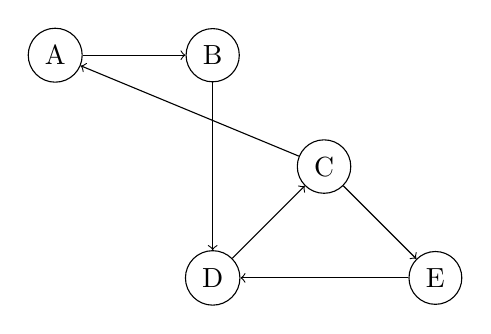
\begin{tikzpicture}[node distance={20mm}, main/.style = {draw, circle}] 
\node[main] (A) {A}; 
\node[main] (B) [right of=A] {B}; 
\node[main] (C) [below right of=B] {C}; 
\node[main] (D) [below left of=C] {D}; 
\node[main] (E) [below right of=C] {E}; 

\draw[->] (A) -- (B);
\draw[->] (B) -- (D);
\draw[->] (D) -- (C);
\draw[->] (C) -- (A);
\draw[->] (C) -- (E);
\draw[->] (E) -- (D);
\end{tikzpicture}
\caption{Directed Graph Example}
\end{figure}
\FloatBarrier

Now, let's apply Kosaraju's algorithm to find the strongly connected components of $G$.
\FloatBarrier
\textbf{Python Code Equivalent}
\FloatBarrier
Here is the Python code equivalent to implement Kosaraju's algorithm:
\FloatBarrier
\begin{lstlisting}
# Python implementation of Kosaraju's Algorithm

def dfs(graph, vertex, visited, stack):
    visited.add(vertex)
    for neighbor in graph[vertex]:
        if neighbor not in visited:
            dfs(graph, neighbor, visited, stack)
    stack.append(vertex)

def transpose_graph(graph):
    transposed = {v: [] for v in graph.keys()}
    for vertex in graph:
        for neighbor in graph[vertex]:
            transposed[neighbor].append(vertex)
    return transposed

def kosaraju(graph):
    visited = set()
    stack = []

    for vertex in graph:
        if vertex not in visited:
            dfs(graph, vertex, visited, stack)

    transposed = transpose_graph(graph)
    visited.clear()
    scc = []

    while stack:
        vertex = stack.pop()
        if vertex not in visited:
            component = []
            dfs(transposed, vertex, visited, component)
            scc.append(component)

    return scc

# Example directed graph G
graph = {
    'A': ['B'],
    'B': ['D'],
    'C': ['A', 'E'],
    'D': ['C'],
    'E': ['D']
}

print("Strongly Connected Components:")
print(kosaraju(graph))
\end{lstlisting}
\FloatBarrier

\subsubsection{Tarjan's Strongly Connected Components Algorithm}
Tarjan's algorithm is used to find strongly connected components in a directed graph. Strongly connected components are subsets of vertices where each vertex is reachable from every other vertex within that subset.

\textbf{Algorithmic Example}
\FloatBarrier
\begin{algorithm}
\caption{Tarjan's Strongly Connected Components Algorithm}\label{tarjan}
\begin{algorithmic}[1]
\State Initialize $index=0$, $S=\emptyset$, $result=\emptyset$
\Function{StrongConnect}{v}
    \State $v.index \gets index$
    \State $v.lowlink \gets index$
    \State $index \gets index + 1$
    \State $S.push(v)$
    \For{each neighbour $w$ of $v$}
        \If{$w.index$ is not defined}
            \State \Call{StrongConnect}{$w$}
            \State $v.lowlink \gets \min(v.lowlink, w.lowlink)$
        \ElsIf{$w$ is in $S$}
            \State $v.lowlink \gets \min(v.lowlink, w.index)$
        \EndIf
    \EndFor
    \If{$v.lowlink = v.index$}
        \State Create a new component $C$
        \Repeat
            \State $w \gets S.pop()$
            \State Add $w$ to $C$
        \Until{$w = v$}
        \State Add $C$ to $result$
    \EndIf
\EndFunction
\end{algorithmic}
\end{algorithm}
\FloatBarrier

\section{Minimum Cut and Graph Partitioning}

Minimum Cut in a graph refers to the partitioning of the vertices of a graph into two sets such that the number of edges between the two sets is minimized. This concept is essential in graph theory and has applications in various fields.

One of the popular algorithms used to find the minimum cut in a graph is the Karger's algorithm:
\FloatBarrier
\begin{algorithm}
\caption{Karger's Algorithm for Minimum Cut}
\begin{algorithmic}[1]
\Function{Karger}{$G$}
\While{$|V(G)| > 2$}
    \State Pick a random edge $(u, v)$ uniformly at random from $E(G)$
    \State Merge the vertices $u$ and $v$ into a single vertex
    \State Remove self-loops
\EndWhile
\State \Return the number of remaining edges
\EndFunction
\end{algorithmic}
\end{algorithm}
\FloatBarrier
This algorithm iteratively contracts edges in the graph until only two vertices remain, representing the two partitions. The number of remaining edges after the iterations gives the minimum cut value.

\subsection{The Concept of Minimum Cut}

The concept of minimum cut in a graph refers to the partitioning of the graph into two sets of vertices, such that the number of edges between the two sets is minimized. In other words, the minimum cut represents the smallest number of edges that need to be removed in order to disconnect the graph.

\textbf{Algorithmic Example}
\FloatBarrier
Here is an algorithmic example to find the minimum cut in a graph using the Ford-Fulkerson algorithm:
\FloatBarrier
\begin{algorithm}
\caption{Ford-Fulkerson Algorithm for Minimum Cut}
\begin{algorithmic}
\State Initialize residual graph $Gf$ with capacities and flows
\State Initialize empty cut set $S$
\While{there is a path $p$ from source $s$ to sink $t$ in $Gf$}
    \State Find the minimum residual capacity $c_f$ of path $p$
    \For{each edge $(u,v)$ in path $p$}
        \State Update the flow $f(u,v) = f(u,v) + c_f$ in $Gf$
        \State Update the reverse edge $(v,u)$ with $f(v,u) = f(v,u) - c_f$
        \If{vertex $v$ is reachable from source in $Gf$}
            \State Add vertex $v$ to set $S$
        \EndIf
    \EndFor
\EndWhile
\end{algorithmic}
\end{algorithm}
\FloatBarrier

\subsubsection{Definition and Importance}
Minimum Cut and Graph Partitioning are fundamental concepts in graph theory and computer science. A minimum cut in a graph is the smallest set of edges that, when removed, disconnects the graph into two or more components. It represents the minimal cost required to break the network into isolated components.

Graph partitioning involves dividing a graph into multiple subsets or partitions based on certain criteria. This partitioning is essential in various applications such as network optimization, clustering, and parallel computing. Finding optimal graph partitions can lead to efficient resource allocation and improved performance in various systems.
\FloatBarrier
\begin{algorithm}\label{algo:min_cut}
\caption{Minimum Cut Algorithm}
\begin{algorithmic}[1]
\State Let $G=(V,E)$ be a connected graph
\State Initialize $min\_cut = \infty$
\For{each vertex $v \in V$}
    \State Partition $G$ into two sets: $A = \{v\}$ and $B = V \setminus \{v\}$
    \State Compute the cut size between $A$ and $B$
    \State Update $min\_cut$ if the current cut size is smaller
\EndFor
\State \textbf{return} $min\_cut$
\end{algorithmic}
\end{algorithm}
\FloatBarrier



\subsection{The Random Contraction Algorithm}
The Random Contraction Algorithm is a randomized algorithm used to find a minimum cut in a graph. The algorithm works by randomly "contracting" edges in the graph until only two vertices remain. The remaining edges between the two vertices form the minimum cut of the graph.
\FloatBarrier

\subsubsection{Algorithm Description}
\begin{algorithm}
\caption{Random Contraction Algorithm}
\begin{algorithmic}[1]
\Function{RandomContraction}{$G$}
    \While{$|V(G)| > 2$}
    \State Pick a random edge $(u,v)$ from $G$
    \State Merge vertices $u$ and $v$ into a single vertex
    \State Remove self-loops
    \EndWhile
\EndFunction
\end{algorithmic}
\end{algorithm}
\FloatBarrier
The algorithm operates by choosing a random edge at each iteration, merging its two endpoints into a single vertex, and removing self-loops until only two vertices remain.

\FloatBarrier
\subsubsection{Analysis and Applications}
The Random Contraction Algorithm is an efficient algorithm for finding the minimum cut in a graph. It works by repeatedly contracting random edges in the graph until there are only two vertices left, representing the two sides of the cut. This algorithm is simple to implement and has applications in various fields such as network analysis, image segmentation, and community detection.

\section{Randomized Algorithms in Graph Theory}
\subsection{Introduction to Randomized Algorithms}

Randomized algorithms in graph theory play a crucial role in solving various graph-related problems efficiently. These algorithms often use randomness in their decision-making process to achieve better performance or to simplify complex computations.
\FloatBarrier
\textbf{Example of a Randomized Algorithm}
One popular randomized algorithm in graph theory is Randomized Primality testing, also known as the Miller-Rabin primality test. The Miller-Rabin test is used to test whether a given number is prime or composite with high probability.
\subsection{Randomized Selection Algorithm}
\subsubsection{Algorithm Overview}
\FloatBarrier
\begin{algorithm}
\caption{Miller-Rabin Primality Test}
\begin{algorithmic}[1]
\Function{MillerRabin}{$n, k$}
    \State Let $d = n-1$
    \State Let $s = 0$
    \While{$d \mod 2 == 0$}
        \State $d \gets d / 2$
        \State $s \gets s + 1$
    \EndWhile
    \For{$i=1$ to $k$}
        \State Choose a random integer $a$ such that $2 \leq a \leq n-2$
        \State $x \gets a^d \mod n$
        \If{$x == 1$ or $x == n-1$}
            \State \textbf{continue}
        \EndIf
        \State $prime \gets$ \textbf{False}
        \For{$r=1$ to $s-1$}
            \State $x \gets x^2 \mod n$
            \If{$x == 1$}
                \State \textbf{return} \textbf{False} \Comment{$n$ is composite}
            \EndIf
            \If{$x == n-1$}
                \State \textbf{break}
            \EndIf
        \EndFor
        \If{$x \neq n-1$}
            \State \textbf{return} \textbf{False} \Comment{$n$ is composite}
        \EndIf
    \EndFor
    \State \textbf{return} \textbf{True} \Comment{$n$ is probably prime}
\EndFunction
\end{algorithmic}
\end{algorithm}

\FloatBarrier
\subsubsection{Analysis}
Randomized selection algorithms are fundamental in computer science and are often used to find the $k$th smallest element in an unsorted array. These algorithms are based on the principle of selecting a pivot element randomly and partitioning the array around this pivot.

The key idea behind randomized selection is that by choosing the pivot randomly, we can avoid the worst-case scenarios encountered in deterministic selection algorithms.

The analysis of randomized selection algorithms involves understanding the expected time complexity and the probability of selecting a good pivot. While the worst-case time complexity of randomized selection algorithms is linear, their expected time complexity is often sublinear.

Let $T(n)$ denote the expected time complexity of selecting the $k$th smallest element in an array of size $n$. The recurrence relation for the expected time complexity can be expressed as:

\[
T(n) = O(n) + T\left(\frac{n}{2}\right)
\]

This recurrence relation arises from the partitioning step of the algorithm, where we divide the array into two subarrays of approximately equal size.

\subsubsection{Applications in Graph Algorithms}

Randomized selection algorithms are powerful tools in graph theory, known for their efficiency and effectiveness in solving complex problems. Here's how they are commonly applied:

\textbf{Randomized Minimum Cut Algorithm}
This approach uses a randomized algorithm to determine a graph's minimum cut efficiently. By randomly selecting edges and contracting them until only two vertices are left, the algorithm finds the minimum cut as the edges connecting these final two vertices.

\textbf{Randomized Approximation Algorithms}
For problems like the maximum cut, graph coloring, and traveling salesman problem, randomized algorithms offer approximation solutions that are often near-optimal. They are particularly valuable for handling large-scale graphs where exact solutions would be computationally prohibitive.

\textbf{Randomized Graph Partitioning}
In graph partitioning, the objective is to split a graph into subgraphs while minimizing the edges cut. Randomized selection algorithms facilitate this by randomly picking vertices or edges to form partitions, making the process efficient and scalable.

\textbf{Randomized Sampling}
These algorithms are also utilized for sampling within large graphs. Randomly selected vertices or edges can provide insights into the overall structure of the graph, aiding tasks like community detection, anomaly identification, and visualization.

These applications underscore the broad utility of randomized selection algorithms in graph theory, offering solutions that balance efficiency with accuracy across various graph-related challenges.


\section{Graph Search Strategies}
Graph search strategies are algorithms used to traverse or search a graph in order to find a particular vertex or a path between two vertices. Some common graph search strategies include Depth-First Search (DFS) and Breadth-First Search (BFS).

\subsection{Cycle Detection and Graph Connectivity}

Cycle detection and graph connectivity are fundamental concepts in graph theory, crucial for understanding the structure and behavior of networks. This subsection focuses on algorithms for detecting cycles in directed and undirected graphs and explores connectivity in graphs, including connected components and strongly connected components.

\subsubsection{Algorithms for Detecting Cycles in Directed and Undirected Graphs}

Detecting cycles in graphs is important for various applications, including deadlock detection in operating systems, circuit design, and verifying the correctness of workflows.

\textbf{Cycle Detection in Directed Graphs:}
One common algorithm for detecting cycles in directed graphs is the Depth-First Search (DFS)-based approach. This method involves tracking the recursion stack during DFS traversal. If a back edge is found (i.e., an edge pointing to an ancestor in the DFS tree), a cycle exists.

\begin{algorithm}[H]
\caption{Cycle Detection in Directed Graphs using DFS}
\begin{algorithmic}[1]
\Function{DFS-Visit}{vertex $v$}
    \State Mark $v$ as visited
    \State Add $v$ to the recursion stack
    \For{each neighbor $u$ of $v$}
        \If{$u$ is not visited}
            \State \Call{DFS-Visit}{$u$}
        \ElsIf{$u$ is in the recursion stack}
            \State \Return True \Comment{Cycle detected}
        \EndIf
    \EndFor
    \State Remove $v$ from the recursion stack
    \Return False
\EndFunction
\Function{HasCycle}{graph $G$}
    \State Initialize visited and recursion stack arrays
    \For{each vertex $v$ in $G$}
        \If{$v$ is not visited}
            \If{\Call{DFS-Visit}{$v$}}
                \State \Return True
            \EndIf
        \EndIf
    \EndFor
    \Return False
\EndFunction
\end{algorithmic}
\end{algorithm}

\textbf{Cycle Detection in Undirected Graphs:}
For undirected graphs, the DFS-based approach can be slightly modified. During DFS traversal, if an adjacent vertex is visited and is not the parent of the current vertex, a cycle is detected.

\begin{algorithm}[H]
\caption{Cycle Detection in Undirected Graphs using DFS}
\begin{algorithmic}[1]
\Function{DFS-Visit}{vertex $v$, parent $p$}
    \State Mark $v$ as visited
    \For{each neighbor $u$ of $v$}
        \If{$u$ is not visited}
            \If{\Call{DFS-Visit}{$u$, $v$}}
                \State \Return True
            \EndIf
        \ElsIf{$u \neq p$}
            \State \Return True \Comment{Cycle detected}
        \EndIf
    \EndFor
    \Return False
\EndFunction
\Function{HasCycle}{graph $G$}
    \State Initialize visited array
    \For{each vertex $v$ in $G$}
        \If{$v$ is not visited}
            \If{\Call{DFS-Visit}{$v$, $-1$}}
                \State \Return True
            \EndIf
        \EndIf
    \EndFor
    \Return False
\EndFunction
\end{algorithmic}
\end{algorithm}

\subsubsection{Connectivity in Graphs: Connected Components and Strongly Connected Components}

Understanding the connectivity of a graph is essential for analyzing its structure and functionality. Connectivity can be categorized into connected components for undirected graphs and strongly connected components for directed graphs.

\textbf{Connected Components:}
In an undirected graph, a connected component is a maximal set of vertices such that there is a path between any two vertices in the set. The DFS or Breadth-First Search (BFS) algorithms can be used to find all connected components by iterating over all vertices and marking all reachable vertices from each unvisited vertex.

\begin{algorithm}[H]
\caption{Finding Connected Components using DFS}
\begin{algorithmic}[1]
\Function{DFS}{vertex $v$}
    \State Mark $v$ as visited
    \For{each neighbor $u$ of $v$}
        \If{$u$ is not visited}
            \State \Call{DFS}{$u$}
        \EndIf
    \EndFor
\EndFunction
\Function{FindConnectedComponents}{graph $G$}
    \State Initialize visited array
    \State Initialize component count to 0
    \For{each vertex $v$ in $G$}
        \If{$v$ is not visited}
            \State Increment component count
            \State \Call{DFS}{$v$}
        \EndIf
    \EndFor
    \Return component count
\EndFunction
\end{algorithmic}
\end{algorithm}

\textbf{Strongly Connected Components:}
In a directed graph, a strongly connected component (SCC) is a maximal subset of vertices such that there is a directed path between any two vertices in the subset. The Kosaraju's or Tarjan's algorithms are commonly used to find SCCs.

\begin{algorithm}[H]
\caption{Finding Strongly Connected Components using Kosaraju's Algorithm}
\begin{algorithmic}[1]
\Function{DFS-FirstPass}{vertex $v$}
    \State Mark $v$ as visited
    \For{each neighbor $u$ of $v$}
        \If{$u$ is not visited}
            \State \Call{DFS-FirstPass}{$u$}
        \EndIf
    \EndFor
    \State Push $v$ onto stack
\EndFunction
\Function{DFS-SecondPass}{vertex $v$}
    \State Mark $v$ as visited
    \For{each neighbor $u$ of $v$ in transpose graph}
        \If{$u$ is not visited}
            \State \Call{DFS-SecondPass}{$u$}
        \EndIf
    \EndFor
\EndFunction
\Function{Kosaraju}{graph $G$}
    \State Initialize stack and visited array
    \For{each vertex $v$ in $G$}
        \If{$v$ is not visited}
            \State \Call{DFS-FirstPass}{$v$}
        \EndIf
    \EndFor
    \State Transpose the graph $G$
    \State Initialize visited array
    \While{stack is not empty}
        \State Pop $v$ from stack
        \If{$v$ is not visited}
            \State \Call{DFS-SecondPass}{$v$}
        \EndIf
    \EndWhile
\EndFunction
\end{algorithmic}
\end{algorithm}


\subsection{Heuristic Search Algorithms in Graphs}
Heuristic search algorithms are a class of algorithms used to solve problems in a more efficient manner by using heuristics. In graph theory, heuristic search algorithms play a crucial role in finding optimal or near-optimal solutions for various graph-related problems. These algorithms leverage heuristic information to guide the search process towards solutions.
\subsubsection{A* Search Algorithm}
One commonly used heuristic search algorithm in graph theory is the A* algorithm. A* is an informed search algorithm that uses both the cost to reach a node (denoted by g) and a heuristic estimation of the cost to reach the goal node from the current node (denoted by h) to determine the next node to explore.

\FloatBarrier
\textbf{Algorithmic example with mathematical detail:}
\FloatBarrier
\begin{algorithm}
    \caption{A* Algorithm}
    \begin{algorithmic}[1]
        \State Initialize an open list with the initial node
        \State Initialize an empty set of explored nodes
        \While{open list is not empty}
            \State Choose the node with the lowest value of f = g + h from the open list
            \State Move this node to the explored nodes set
            \If{current node is the goal node}
                \State \textbf{return} path
            \EndIf
            \For{each neighbor of the current node}
                \If{neighbor is not in the open list or explored nodes}
                    \State Calculate g and h values for the neighbor
                    \State Add the neighbor to the open list
                \EndIf
            \EndFor
        \EndWhile
    \end{algorithmic}
\end{algorithm}
\FloatBarrier


\subsubsection{Greedy Best-First Search}
Greedy Best-First Search is a variation of Best-First Search algorithm that prioritizes nodes based on a heuristic evaluation function. At each step, it selects the node that appears to be the most promising based on the heuristic.
\FloatBarrier
\textbf{Algorithm}
\FloatBarrier
\begin{algorithm}
\caption{Greedy Best-First Search}
\begin{algorithmic}
\State \textbf{Input:} Graph $G$, start node $s$, heuristic function $h$
\State \textbf{Output:} Path from $s$ to goal node

\State Initialize priority queue $Q$ with $s$
\State Initialize an empty set $visited$
\While{$Q$ is not empty}
    \State $current \gets Q$.pop()
    \If{$current$ is goal node}
        \State \textbf{return} path to $current$
    \EndIf
    \State Add $current$ to $visited$
    \For{each neighbor $n$ of $current$}
        \If{$n$ is not in $visited$}
            \State Calculate priority $p$ using heuristic function: $p = h(n)$
            \State Add $n$ to $Q$ with priority $p$
        \EndIf
    \EndFor
\EndWhile
\State \textbf{return} No path found
\end{algorithmic}
\end{algorithm}

\section{Graph Path Finding Algorithms}
Graph path finding algorithms are a set of techniques to find the shortest path between nodes in a graph. These algorithms are essential in various applications like navigation systems, network routing, and social network analysis.

One of the well-known algorithms for solving shortest path problems is Dijkstra's algorithm. This algorithm finds the shortest path from a starting node to all other nodes in a weighted graph. It uses a priority queue to greedily select the node with the smallest distance at each step until all nodes have been visited.

\subsection{Shortest Path Algorithms}
Shortest path algorithms are crucial in graph theory for finding the quickest route between two vertices in a weighted graph. These algorithms are widely used in network routing, transportation planning, and other optimization scenarios where the goal is to minimize travel cost or distance.

\textbf{Dijkstra's Algorithm}
One of the most renowned shortest path algorithms is Dijkstra's algorithm. Developed by Edsger W. Dijkstra in 1956, it efficiently computes the shortest paths from a single source vertex to all other vertices in a graph with non-negative edge weights. Dijkstra's algorithm uses a priority queue to keep track of vertex distances and iteratively updates the paths and distances until all vertices are processed.

\textbf{Bellman-Ford Algorithm}
For graphs that include negative edge weights, the Bellman-Ford algorithm is more suitable. It iterates over the graph's edges to minimize the path distances, also providing the capability to detect negative cycles, which are crucial for understanding feasibility and stability in networks.

\textbf{Specialized Algorithms}
Other algorithms like the A* algorithm cater to graphs with non-negative integer weights by utilizing heuristics to speed up the search, whereas the Floyd-Warshall algorithm addresses scenarios with negative weights by finding shortest paths between all pairs of vertices.

\subsubsection{Dijkstra's Algorithm in Detail}
Dijkstra's algorithm operates as follows:
- Initialize distances: Set the distance from the source to itself to zero and all others to infinity.
- Use a priority queue: Store vertices by distance from the source.
- Relax edges: For the vertex with the shortest distance in the queue, update the distances for its adjacent vertices.
- Repeat: Continue until all vertices are processed.

The result is a set of shortest paths from the source to all vertices, enabling efficient route planning and network design.

Overall, shortest path algorithms like Dijkstra's provide essential tools for designing and optimizing systems across various fields, enhancing the efficiency of resources and operational planning.


Here is the implementation of Dijkstra's algorithm in Python:
\FloatBarrier
\begin{lstlisting}
    import heapq

def dijkstra(graph, source):
    # Initialize distances to all vertices as infinity
    distances = {vertex: float('infinity') for vertex in graph}
    distances[source] = 0
    
    # Priority queue to store vertices sorted by distance
    pq = [(0, source)]
    
    while pq:
        current_distance, current_vertex = heapq.heappop(pq)
        
        # Skip if the current distance is greater than the known distance
        if current_distance > distances[current_vertex]:
            continue
            
        # Iterate over neighbors of the current vertex
        for neighbor, weight in graph[current_vertex].items():
            distance = current_distance + weight
            
            # Relax the edge if a shorter path is found
            if distance < distances[neighbor]:
                distances[neighbor] = distance
                heapq.heappush(pq, (distance, neighbor))
    
    return distances
\end{lstlisting}
In this implementation, graph is a dictionary representing the weighted graph, where keys are vertices and values are dictionaries of neighbors and their corresponding edge weights. source is the starting vertex for which the shortest paths are to be computed. The function returns a dictionary containing the shortest distances from the source vertex to all other vertices in the graph.

\subsubsection{Bellman-Ford Algorithm}
The Bellman-Ford algorithm, developed by Richard Bellman and Lester Ford Jr. in the 1950s, finds shortest paths from a single source vertex to all other vertices in a weighted graph. This method is particularly valuable because it can handle graphs with negative weight edges, a feature not supported by Dijkstra's algorithm.

\textbf{How It Works:}
The Bellman-Ford algorithm operates through a process called edge relaxation, which iteratively updates the shortest path estimates:

- \textbf{Initialization:} Set the distance from the source vertex to itself to zero and all other vertex distances to infinity.

- \textbf{Edge Relaxation:} For \(|V|-1\) iterations—where \(|V|\) is the number of vertices—relax all the edges. This involves checking each edge and, if a shorter path is found, updating the distance estimate for the vertex at the end of that edge.

- \textbf{Negative Cycle Detection:} After \(|V|-1\) cycles, any further ability to relax an edge indicates a negative weight cycle in the graph.

\textbf{Practical Implications:}
Though less efficient than Dijkstra's algorithm due to its need to relax edges multiple times, Bellman-Ford is crucial for applications where negative weights are involved and there's a need to ensure no negative cycles exist. The algorithm guarantees that the shortest paths calculated after \(|V|-1\) iterations are optimal unless a negative cycle affects the distances.

By providing a method to handle complex edge weight configurations, the Bellman-Ford algorithm remains a fundamental tool for network design and analysis, ensuring robust route planning even under challenging conditions.


Here's the Python implementation of the Bellman-Ford algorithm:
\FloatBarrier
\begin{lstlisting}
    def bellman_ford(graph, source):
    # Step 1: Initialize distances
    distances = {vertex: float('infinity') for vertex in graph}
    distances[source] = 0
    
    # Step 2: Relax edges for |V| - 1 iterations
    for _ in range(len(graph) - 1):
        for u, edges in graph.items():
            for v, weight in edges.items():
                if distances[u] + weight < distances[v]:
                    distances[v] = distances[u] + weight
    
    # Step 3: Check for negative weight cycles
    for u, edges in graph.items():
        for v, weight in edges.items():
            if distances[u] + weight < distances[v]:
                raise ValueError("Graph contains negative weight cycle")
    
    return distances
\end{lstlisting}
\FloatBarrier
In this implementation, graph is a dictionary representing the weighted graph, where keys are vertices and values are dictionaries of neighbors and their corresponding edge weights. source is the starting vertex for which the shortest paths are to be computed. The function returns a dictionary containing the shortest distances from the source vertex to all other vertices in the graph, or raises an error if a negative weight cycle is detected.

\subsection{All-Pairs Shortest Paths}
The "All-Pairs Shortest Paths" problem is pivotal in graph theory and deals with finding the shortest path between every pair of vertices in a weighted graph. This task is essential in various applications like network routing, transportation planning, and social network analysis, where understanding the shortest distances between all nodes is crucial for optimization and planning.

\textbf{Floyd-Warshall Algorithm}
A key tool for solving this problem is the Floyd-Warshall algorithm, renowned for its efficiency with dense graphs. It utilizes dynamic programming to iteratively refine the shortest path distances between all vertex pairs. The algorithm keeps a matrix that records these distances and updates it by considering whether taking paths through intermediate vertices offers a shorter path between any two vertices.

\textbf{Johnson's Algorithm}
For sparser graphs, Johnson's algorithm provides a more suitable alternative. It cleverly merges the approaches of Dijkstra’s and Bellman-Ford algorithms, accommodating graphs with negative edge weights while efficiently handling sparse connections.

\textbf{Applications and Practical Importance}
From optimizing data flow between routers in communication networks to reducing travel times in urban planning, the solutions to the All-Pairs Shortest Paths problem play a foundational role. They not only enhance efficiency in real-world networks but also contribute to more robust and effective system designs.

\subsubsection{Floyd-Warshall Algorithm in Detail}
Independently developed by Bernard Roy and Stephen Warshall in the early 1960s and refined by Robert Floyd, the Floyd-Warshall algorithm is a cornerstone in computing shortest paths in weighted graphs. This algorithm performs particularly well in graphs that can have negative edge weights but must be free of negative weight cycles.

\textbf{Operation:}
The algorithm updates a distance matrix by systematically checking all possible paths through each vertex to see if a shorter path exists, using a methodical dynamic programming approach. It requires \(O(V^3)\) time complexity, where \(V\) is the number of vertices, making it especially suitable for graphs where the vertex count isn't prohibitively large.

\textbf{Significance:}
This method’s ability to compute shortest paths between all pairs of vertices simultaneously makes it invaluable for analyses where every inter-node distance is critical, supporting thorough and efficient evaluations of complex networks.


Here are the main steps of the Floyd-Warshall algorithm:

\begin{enumerate}
    \item Initialize a $|V| \times |V|$ matrix distances to represent the shortest distances between all pairs of vertices. Initially, the matrix is filled with the weights of the edges in the graph, and the diagonal elements are set to 0.
    \item For each intermediate vertex $k$ from 1 to $|V|$, iterate over all pairs of vertices $(i, j)$ and update the \texttt{distances[i][j]} entry if the path through vertex $k$ produces a shorter distance.
    \item After the iterations are complete, the \texttt{distances} matrix will contain the shortest distances between all pairs of vertices in the graph.
\end{enumerate}

\textbf{Python Implementation:}
\FloatBarrier
\begin{lstlisting}
    def floyd_warshall(graph):
    # Initialize the distance matrix
    distances = {u: {v: float('inf') for v in graph} for u in graph}
    for u in graph:
        distances[u][u] = 0
    for u in graph:
        for v, weight in graph[u].items():
            distances[u][v] = weight
    
    # Update distances using Floyd-Warshall algorithm
    for k in graph:
        for u in graph:
            for v in graph:
                distances[u][v] = min(distances[u][v], distances[u][k] + distances[k][v])
    
    return distances
\end{lstlisting}
In this implementation, graph is a dictionary representing the weighted graph, where keys are vertices and values are dictionaries of neighbors and their corresponding edge weights. The function returns a nested dictionary containing the shortest distances between all pairs of vertices in the graph.

\subsubsection{Johnson's Algorithm}
Johnson's algorithm is used to find the shortest paths between all pairs of vertices in a weighted graph, even in the presence of negative edge weights and negative weight cycles. It was developed by Donald B. Johnson in 1977. Johnson's algorithm combines Dijkstra's algorithm with the Bellman-Ford algorithm to handle negative edge weights.

Here's how Johnson's algorithm works:

\begin{enumerate}
    \item Add a new vertex, called the "dummy vertex," to the graph and connect it to all other vertices with zero-weight edges. This transforms the original graph into a new graph with no negative edge weights.
    \item Run the Bellman-Ford algorithm on the new graph with the dummy vertex as the source. This step detects negative weight cycles, if any.
    \item If the Bellman-Ford algorithm detects a negative weight cycle, terminate the algorithm and report that the graph contains a negative weight cycle.
    \item If there are no negative weight cycles, reweight the edges of the original graph using vertex potentials computed during the Bellman-Ford algorithm.
    \item For each vertex in the original graph, run Dijkstra's algorithm to find the shortest paths to all other vertices. Use the reweighted edge weights obtained in step 4.
    \item After running Dijkstra's algorithm for all vertices, compute the shortest paths between all pairs of vertices based on the distances obtained.
\end{enumerate}
\FloatBarrier
\textbf{Python Implementation:}
\FloatBarrier
\begin{lstlisting}
    import heapq
from collections import defaultdict

def bellman_ford(graph, source):
    distance = {v: float('inf') for v in graph}
    distance[source] = 0
    for _ in range(len(graph) - 1):
        for u, neighbors in graph.items():
            for v, weight in neighbors.items():
                distance[v] = min(distance[v], distance[u] + weight)
    return distance

def dijkstra(graph, source):
    distances = {v: float('inf') for v in graph}
    distances[source] = 0
    heap = [(0, source)]
    while heap:
        dist_u, u = heapq.heappop(heap)
        if dist_u > distances[u]:
            continue
        for v, weight in graph[u].items():
            if distances[u] + weight < distances[v]:
                distances[v] = distances[u] + weight
                heapq.heappush(heap, (distances[v], v))
    return distances

def johnson(graph):
    # Step 1: Add a dummy vertex and connect it to all other vertices with zero-weight edges
    dummy = 'dummy'
    graph[dummy] = {v: 0 for v in graph}

    # Step 2: Run Bellman-Ford algorithm to detect negative weight cycles and compute vertex potentials
    potentials = bellman_ford(graph, dummy)
    if any(potentials[v] < 0 for v in graph):
        return "Negative weight cycle detected"

    # Step 3: Reweight the edges using vertex potentials
    for u, neighbors in graph.items():
        for v in neighbors:
            graph[u][v] += potentials[u] - potentials[v]

    # Step 4: Run Dijkstra's algorithm for each vertex to find shortest paths to all other vertices
    shortest_paths = {}
    for u in graph:
        shortest_paths[u] = dijkstra(graph, u)

    # Step 5: Restore original distances using vertex potentials
    for u, distances in shortest_paths.items():
        for v in distances:
            shortest_paths[u][v] += potentials[v] - potentials[u]

    return shortest_paths
\end{lstlisting}
\FloatBarrier
This implementation returns a dictionary containing the shortest paths between all pairs of vertices in the graph. If a negative weight cycle is detected, the function returns the message "Negative weight cycle detected."

\section{Network Flow and Matching}
Network Flow and Matching are fundamental concepts in graph theory and algorithms. In the context of network flow, the goal is to determine how to optimally transport items through a network, while in matching, the objective is to find pairings or matchings between elements of different sets that satisfy certain criteria.

\subsection{Maximum Flow Problem}
The Maximum Flow Problem is a fundamental problem in graph theory and network flow optimization. Given a directed graph with capacities on the edges, the goal is to find the maximum amount of flow that can be sent from a source node to a sink node. This problem has various applications in transportation, communication networks, and more.

\textbf{Algorithmic Example}
\FloatBarrier
The Ford-Fulkerson algorithm is a popular algorithm for solving the Maximum Flow Problem. It iteratively finds augmenting paths from the source to the sink and increases the flow along these paths until no more augmenting paths can be found. The algorithm terminates when no more augmenting paths exist, and the flow is maximized.
\FloatBarrier
\begin{algorithm}
\caption{Ford-Fulkerson Algorithm}
\begin{algorithmic}
\Require Directed graph $G$, source node $s$, sink node $t$
\Ensure Maximum flow value $max\_flow$
\Function{FordFulkerson}{$G, s, t$}
    \State Initialize flow $f$ on all edges to 0
    \State $max\_flow \gets 0$
    \While{there exists an augmenting path $p$ from $s$ to $t$ in residual graph $G_f$}
        \State Find the bottleneck capacity $c_f(p)$ of path $p$
        \State Augment flow $f$ along path $p$
        \State Update residual capacities in $G_f$
        \State Update $max\_flow$ with $c_f(p)$
    \EndWhile
    \State \Return $max\_flow$
\EndFunction
\end{algorithmic}
\end{algorithm}
\FloatBarrier

\subsubsection{Edmonds-Karp Algorithm}
The Edmonds-Karp Algorithm is a specific implementation of the Ford-Fulkerson method for computing the maximum flow in a flow network. It uses the concept of augmenting paths to iteratively find the maximum flow from a source vertex to a sink vertex in a flow network.
\FloatBarrier
\textbf{Algorithmic example for the Edmonds-Karp Algorithm:}
\FloatBarrier
\begin{algorithm}
\caption{Edmonds-Karp Algorithm}
\begin{algorithmic}[1]
\State Initialize flow network $G$ with capacities and flow values
\State Initialize maximum flow $0$
\While{there exists an augmenting path $p$ from source $s$ to sink $t$ in residual network $G_f$}
    \State Find the minimum residual capacity along path $p$ as $c_f(p)$
    \State Update the flow along path $p$ by adding $c_f(p)$ to $f$
    \State Update the residual capacities and flow values of edges in $p$
    \State Update the maximum flow with $c_f(p)$
\EndWhile
\end{algorithmic}
\end{algorithm}
\FloatBarrier


\subsection{Minimum Cost Flow Problem}
The minimum cost flow problem is a network optimization problem where the goal is to find the cheapest way to send a certain amount of flow through a flow network. Each edge in the network has a capacity (maximum flow that can pass through it) and a cost per unit of flow. The objective is to minimize the total cost of sending the required flow from a source node to a sink node.
\FloatBarrier
\textbf{Algorithmic Example}
\FloatBarrier
Let's consider a simple example where we have a flow network represented by a directed graph with nodes $s$ as the source and $t$ as the sink. Each edge in the graph has a capacity and a cost associated with it. We want to find the minimum cost to send a certain amount of flow $F$ from $s$ to $t$.

We can solve this problem using the Minimum Cost Flow algorithm, which is based on the Ford-Fulkerson method with the Bellman-Ford shortest path algorithm for finding the minimum cost.
\FloatBarrier
\begin{algorithm}
\caption{Minimum Cost Flow Algorithm}
\begin{algorithmic}[1]
\State Initialize flow on each edge to 0
\State While there exists a path from $s$ to $t$ with available capacity:
\State \hspace{10mm} Find the path with the minimum cost using Bellman-Ford
\State \hspace{10mm} Update the flow along the path
\State Calculate the total cost as the sum of costs of all edges with non-zero flow
\end{algorithmic}
\end{algorithm}
\FloatBarrier

\subsubsection{Applications and Solutions}
The minimum cost flow problem is a fundamental problem in optimization theory with various practical applications. Some common applications include:
\begin{itemize}
    \item Transportation and logistics planning: Optimizing the flow of goods through a network while minimizing transportation costs.
    \item Communication network design: Finding the most cost-effective way to route data through a network.
    \item Supply chain management: Determining the optimal distribution of resources from suppliers to consumers.
\end{itemize}
\FloatBarrier


\section{Conclusion}
\subsection{Summary of Graph Algorithms}
Graph algorithms are used to analyze relationships between elements in a graph. They can be used to solve various problems such as finding the shortest path, determining connectivity, identifying cycles, and more. Here, we provide an example of a basic graph algorithm.

\subsection{Challenges in Graph Algorithm Research}
Graph algorithm research faces several challenges, including:

1. \textbf{Scalability}: As graphs grow larger in scale and complexity, algorithm efficiency becomes crucial. Developing algorithms that can handle massive graphs efficiently is a significant challenge.

2. \textbf{Dynamic Graphs}: Real-world graphs often evolve over time, with edges and vertices being added or removed dynamically. Designing algorithms that can adapt to such changes and maintain correctness is a challenging area of research.

3. \textbf{Complexity Analysis}: Analyzing the complexity of graph algorithms and determining their time and space complexity is not always straightforward, especially for algorithms dealing with highly connected or dense graphs.

\subsection{Future Directions in Graph Theory and Algorithm Research}
Graph theory and algorithms have been extensively studied and applied in various fields like computer science, mathematics, and network analysis. There are several exciting future directions for research in this area. One such direction is the development of algorithms for handling massive graphs efficiently. With the growth of data, analyzing and processing large-scale graphs poses a significant challenge.

Another promising avenue is the exploration of new graph properties and structures that can lead to the development of innovative graph algorithms. Additionally, integrating graph theory with other fields such as machine learning and data science opens up new possibilities for advanced applications and research.


\section{Further Reading and Resources}
To deepen your understanding of graph algorithms, there are numerous resources available that range from academic papers and books to online tutorials and open-source libraries. This section provides a comprehensive guide to these resources, helping you explore the topic in greater detail and apply what you have learned to real-world problems.

\subsection{Key Papers and Books on Graph Algorithms}
A solid foundation in graph algorithms can be built by studying some of the key papers and books in the field. These resources provide both theoretical insights and practical applications.

\begin{itemize}
    \item \textbf{“Graph Theory” by Reinhard Diestel} - This book is a comprehensive introduction to graph theory, covering fundamental concepts and theorems.
    \item \textbf{“Introduction to Algorithms” by Thomas H. Cormen, Charles E. Leiserson, Ronald L. Rivest, and Clifford Stein} - Often referred to as CLRS, this book is a must-read for anyone studying algorithms. It includes detailed sections on graph algorithms, such as breadth-first search, depth-first search, and shortest paths.
    \item \textbf{“Network Flows: Theory, Algorithms, and Applications” by Ravindra K. Ahuja, Thomas L. Magnanti, and James B. Orlin} - This book delves into the theory and algorithms related to network flows, providing both theoretical and practical perspectives.
    \item \textbf{“The Annotated Turing” by Charles Petzold} - While not exclusively about graph algorithms, this book offers an insightful look into the foundations of computer science, which underpin many algorithmic concepts.
    \item \textbf{“A Note on Two Problems in Connexion with Graphs” by Leonard Euler} - This seminal paper from 1736 is often considered the starting point of graph theory, introducing the famous Seven Bridges of Königsberg problem.
    \item \textbf{“The Shortest Path Problem” by Edsger W. Dijkstra} - Dijkstra's 1959 paper introduces his algorithm for finding the shortest path in a graph, a fundamental concept in graph theory.
\end{itemize}

\subsection{Online Tutorials and Courses}
Online tutorials and courses offer interactive and accessible ways to learn graph algorithms. These resources often include video lectures, coding exercises, and forums for discussion.

\begin{itemize}
    \item \textbf{Coursera’s “Algorithms” Specialization by Stanford University} - This series of courses covers a wide range of algorithmic topics, including several modules on graph algorithms.
    \item \textbf{edX’s “Algorithms and Data Structures” by IIT Bombay} - This course provides a comprehensive introduction to algorithms and data structures, with a strong emphasis on graph algorithms.
    \item \textbf{MIT OpenCourseWare’s “Introduction to Algorithms”} - MIT’s OCW offers free lecture notes, assignments, and exams for their algorithms course, which includes detailed coverage of graph algorithms.
    \item \textbf{Khan Academy’s “Algorithms” Course} - This course offers a user-friendly introduction to algorithms, including graph traversal techniques and shortest path algorithms.
    \item \textbf{LeetCode and HackerRank} - These platforms provide a plethora of problems and challenges on graph algorithms, allowing students to practice and refine their skills through hands-on coding.
\end{itemize}

\subsection{Open-Source Libraries and Tools for Graph Algorithm Implementation}
Implementing graph algorithms requires practical tools and libraries. Several open-source libraries can help you efficiently implement and test graph algorithms.

\begin{itemize}
    \item \textbf{NetworkX} - A Python library for the creation, manipulation, and study of the structure, dynamics, and functions of complex networks. NetworkX is particularly user-friendly for implementing graph algorithms.


    \item \textbf{Graph-tool} - An efficient Python module for manipulation and statistical analysis of graphs (networks). Graph-tool is designed for performance and scalability.
    \item \textbf{JGraphT} - A Java library that provides mathematical graph-theory objects and algorithms. It is highly versatile and can be used for a wide range of graph-related tasks.
    \item \textbf{Gephi} - An open-source network analysis and visualization software package written in Java. It allows users to interact with the representation, manipulation, and visualization of graphs.
    \item \textbf{Neo4j} - A highly scalable native graph database that leverages data relationships as first-class entities. Neo4j is particularly useful for applications that require efficient querying and manipulation of graph data.
    \item \textbf{igraph} - A collection of network analysis tools with interfaces to R, Python, and C/C++. It is particularly well-suited for large graphs and complex network analyses.
\end{itemize}

These resources will provide you with a robust toolkit for learning, implementing, and exploring graph algorithms. Whether you are just starting or looking to deepen your knowledge, these books, courses, and libraries offer valuable insights and practical skills.


\section{End of Chapter Exercises}
In this section, we provide a comprehensive set of exercises designed to reinforce and apply the concepts learned in this chapter on Graph Algorithm Techniques. These exercises are divided into two main categories: conceptual questions to reinforce learning and practical coding challenges to apply graph algorithm techniques. By completing these exercises, students will deepen their understanding of the material and gain practical experience in implementing and utilizing graph algorithms.

\subsection{Conceptual Questions to Reinforce Learning}
This subsection contains a series of conceptual questions aimed at reinforcing the theoretical understanding of graph algorithms. These questions are intended to test the students' grasp of key concepts, definitions, and properties related to graph theory and graph algorithms.

\begin{itemize}
    \item \textbf{Question 1:} Explain the difference between a directed and an undirected graph. Provide examples of real-world scenarios where each type would be applicable.
    \item \textbf{Question 2:} Define what a spanning tree is in the context of graph theory. How does it relate to a minimum spanning tree?
    \item \textbf{Question 3:} Describe Dijkstra's algorithm for finding the shortest path in a weighted graph. What are its time complexity and limitations?
    \item \textbf{Question 4:} Compare and contrast Depth-First Search (DFS) and Breadth-First Search (BFS) in terms of their methodologies and applications.
    \item \textbf{Question 5:} What is a bipartite graph? Provide a method to determine if a given graph is bipartite.
    \item \textbf{Question 6:} Discuss the concept of graph coloring. What is the chromatic number, and how can it be determined for a graph?
    \item \textbf{Question 7:} Explain the significance of the Bellman-Ford algorithm. In what scenarios is it preferable over Dijkstra's algorithm?
    \item \textbf{Question 8:} Describe the concept of network flow and the Ford-Fulkerson method for computing the maximum flow in a flow network.
\end{itemize}

\chapter{Greedy Algorithms}

\section{Introduction to Greedy Algorithms}
Greedy algorithms are a neat way to solve problems by always making the best choice at the moment. Think of it like picking the ripest fruit each time from a basket to hopefully end up with the best bunch at the end. These algorithms build up solutions step by step, choosing options that seem the best at each step. They work really well for certain types of problems where each of these choices leads us closer to an optimal solution, although they might not always give the perfect answer for every scenario.

\textbf{Algorithmic example:}
\FloatBarrier

\begin{algorithm}
\caption{Greedy Algorithm Example}
\begin{algorithmic}[1]
\State Assume we have a set of $n$ tasks $T = \{t_1, t_2, \ldots, t_n\}$ with respective profits $P = \{p_1, p_2, \ldots, p_n\}$ and deadlines $D = \{d_1, d_2, \ldots, d_n\}$.
\State Sort tasks based on their profits in decreasing order.
\State Initialize schedule $S$ as an empty list.
\For{$i$ from $1$ to $n$}
    \State Insert task $t_i$ into $S$ at the latest possible position without missing its deadline.
\EndFor
\State \textbf{Return} Schedule $S$ with maximum total profit.
\end{algorithmic}
\end{algorithm}

\FloatBarrier

\subsection{Definition and Characteristics}
Greedy algorithms make a series of decisions, where each decision selects the locally optimal choice at that step. The hope is that by picking a locally optimal solution at each step, the algorithm will eventually come up with a global optimum solution.


\textbf{Characteristics of Greedy Algorithms:}
\begin{itemize}
    \item \textbf{Greedy-choice Property}: At each step, a greedy algorithm makes a locally optimal choice that leads to the best possible solution For that step without considering the overall outcome.
    \item \textbf{Optimal Substructure}: The optimal solution to the problem can be obtained by combining the locally optimal choices made at each step.
    \item \textbf{Does not reconsider choices}: Once a decision is made, a greedy algorithm does not revisit or reconsider it. This makes the algorithm efficient but may not always lead to the globally optimal solution
\end{itemize}

\subsection{Principles of Greedy Strategy}
The Greedy Strategy is a simple approach to solving optimization problems by making locally optimal choices at each step with the hope of finding a global optimum. The main principles of the Greedy Strategy are:

\begin{itemize}
    \item \textbf{Greedy Choice Property:} A globally optimal solution can be reached by making a locally optimal choice at each step.
    \item \textbf{Optimal Substructure:} The problem can be broken down into smaller subproblems, and the solution to the overall problem can be constructed from solutions to the subproblems.
\end{itemize}

One classic example of the Greedy Strategy is the \textbf{Coin Change Problem}. Given a set of coin denominations and a target amount, the goal is to find the minimum number of coins needed to make up that amount.

\textbf{Algorithm: Coin Change Problem}
\FloatBarrier
\begin{algorithm}
\caption{Greedy Coin Change Algorithm}
\begin{algorithmic}[1]
\Procedure{GreedyCoinChange}{$\text{coins}[], \text{target}$}
    \State $\text{numCoins} \gets 0$
    \State $\text{index} \gets \text{length}(\text{coins}) - 1$
    \While{$\text{target} > 0$ and $\text{index} \geq 0$}
        \If{$\text{coins}[\text{index}] \leq \text{target}$}
            \State $\text{numCoins} \gets \text{numCoins} + \text{target} \div \text{coins}[\text{index}]$
            \State $\text{target} \gets \text{target} \% \text{coins}[\text{index}]$
        \EndIf
        \State $\text{index} \gets \text{index} - 1$
    \EndWhile
    \State \textbf{Return} $\text{numCoins}$
\EndProcedure
\end{algorithmic}
\end{algorithm}
\FloatBarrier

\textbf{Explanation:}
\begin{itemize}
    \item We start with the highest denomination coin and keep subtracting it from the target amount until it becomes zero or negative.
    \item Then, we move to the next smaller denomination and repeat the process until we reach the smallest denomination or the target amount becomes zero.
    \item At each step, we make the locally optimal choice by choosing the largest denomination that doesn't exceed the remaining target amount.
\end{itemize}

\subsection{Applications and Limitations}
Greedy algorithms are often used in optimization problems where we make a series of choices that result in an optimal solution. One common application is in the scheduling of activities to maximize the number of activities that can be performed within a given time constraint.

\textbf{Algorithmic Example: Activity Selection Problem}
\FloatBarrier
Given a set of activities with start and finish times, the goal is to select the maximum number of non-overlapping activities.
\FloatBarrier
\begin{algorithm}
\caption{Activity Selection Problem}
\begin{algorithmic}[1]
\State Sort activities by finish time
\State Include the first activity in the solution
\For{each activity starting from the second}
    \If{activity start time is greater than or equal to the finish time of the previously selected activity}
        \State Include the activity in the solution
    \EndIf
\EndFor
\end{algorithmic}
\end{algorithm}

\FloatBarrier
This example demonstrates the application of a greedy algorithm For solving the activity selection problem. The algorithm selects activities based on their finish times to maximize the number of non-overlapping activities that can be performed. The provided Python code implements this algorithm For the given set of activities.


Although greedy algorithms are simple and efficient, they may not always provide the optimal solution. Some common limitations of greedy algorithms include:
\begin{itemize}
    \item Greedy algorithms may not always guarantee the globally optimal solution.
    \item They may overlook certain choices that lead to a better solution in the future.
    \item Finding the optimal solution may require considering all possible choices, which greedy algorithms do not always do.
\end{itemize}

To illustrate the limitations of greedy algorithms, let's consider the Fractional Knapsack Problem. 

In this problem, we are given a set of items, each with a weight \( w_i \) and a value \( v_i \), and a knapsack with a maximum weight capacity \( W \). The goal is to fill the knapsack with items to maximize the total value while not exceeding the weight capacity. Unlike the 0/1 Knapsack Problem, where items cannot be divided, in the Fractional Knapsack Problem, we can take fractions of items.

The greedy strategy For the Fractional Knapsack Problem involves selecting items based on their value-to-weight ratios. At each step, we choose the item with the highest value-to-weight ratio and take as much of it as possible until the knapsack is full. However, the greedy approach may not always yield the optimal solution.

Let's demonstrate this with an algorithmic example:

\begin{algorithm}
\caption{Greedy Fractional Knapsack Algorithm}
\begin{algorithmic}[1]
\Procedure{FractionalKnapsack}{items[], W}
    \State Sort items by decreasing value-to-weight ratio
    \State totalValue $\gets$ 0
    \State remainingWeight $\gets$ W
    \For{item in items}
        \If{item.weight $\leq$ remainingWeight}
            \State totalValue $\gets$ totalValue + item.value
            \State remainingWeight $\gets$ remainingWeight - item.weight
        \Else
            \State fraction $\gets$ remainingWeight / item.weight
            \State totalValue $\gets$ totalValue + fraction $\times$ item.value
            \State remainingWeight $\gets$ 0
            \State \textbf{break}
        \EndIf
    \EndFor
    \State \textbf{Return} totalValue
\EndProcedure
\end{algorithmic}
\end{algorithm}

\FloatBarrier

In this algorithm, \texttt{items} is a list of items with their respective weights and values. The algorithm sorts the items in decreasing order of their value-to-weight ratios and iterates through them. At each step, if the entire weight of the current item can fit into the knapsack, it is fully taken. Otherwise, a fraction of the item is taken to fill the remaining capacity.

However, the greedy approach fails For cases where the items' value-to-weight ratios do not reflect their overall contribution to the solution. Consider the following example:

Suppose we have a knapsack with a capacity of 50 units and the following items:

\begin{itemize}
    \item Item 1:
    \[
    \begin{aligned}
    & \text{Weight} = 20, \\
    & \text{Value} = 100 \\
    \end{aligned}
    \]

    \item Item 2:
    \[
    \begin{aligned}
    & \text{Weight} = 30, \\
    & \text{Value} = 120 \\
    \end{aligned}
    \]
\end{itemize}

The greedy algorithm would first select Item 1, taking its full weight since it fits entirely into the knapsack. Then, it would select Item 2, taking its full weight as well. However, this results in a total value of 220, whereas the optimal solution would be to take only Item 2, yielding a total value of 120, which is higher. Therefore, the greedy algorithm fails to find the optimal solution in this case.

\subsection{Efficiency and Correctness}

\textbf{Efficiency}\\
Greedy algorithms are typically fast, which makes them quite appealing when you need to solve big problems quickly. They often work in a linear or nearly linear time, relative to the size of your input, allowing them to handle large-scale tasks smoothly.

\textbf{Correctness}\\
Although greedy algorithms are quick, they don't always promise the best solution possible. Whether they work correctly depends on two main properties:

\begin{description}
    \item[\textbf{Greedy Choice Property:}] This means that making the best local choice at each step of the algorithm will lead you to the best overall solution. It's like trusting that picking the best option now won’t mess up your choices later.
    
    \item[\textbf{Optimal Substructure Property:}] This property tells us that a problem’s best solution is built using the best solutions to smaller versions of the same problem. Essentially, if you can solve smaller parts perfectly, you can stitch these parts together to solve the whole problem perfectly.
\end{description}

\textbf{A Practical Example: The Activity Selection Problem}\\
Let's look at a classic problem that greedy algorithms nail: the Activity Selection Problem. You have a bunch of activities, each with a start and end time, and you want to fit as many as possible without any overlaps. Here's how a greedy algorithm would tackle this:

\begin{itemize}
    \item First, sort the activities by their end times.
    \item Then, keep picking the activity that ends the soonest and doesn't overlap with what you've already picked.
\end{itemize}

The sorting step gives this greedy approach a time complexity of \(O(n \log n)\), where \(n\) is the number of activities. This algorithm works perfectly for this problem because choosing the activity that ends the soonest each time ensures you get the maximum number of non-overlapping activities.

\section{Interval Scheduling}
Interval Scheduling is a classic algorithmic problem that involves scheduling a maximum number of mutually compatible tasks, given a set of tasks with start and finish times. The goal is to select the largest possible subset of mutually non-overlapping tasks.

\subsection{Problem Definition}
Interval Scheduling is a classic problem in algorithm design that involves selecting the maximum number of non-overlapping intervals from a set of intervals. Given a set of intervals with start and end times, the goal is to find the largest subset of non-overlapping intervals.

The problem can be Formally defined as follows: \\
Given a set of n intervals $[s_1, e_1], [s_2, e_2], ..., [s_n, e_n]$, where $s_i$ denotes the start time and $e_i$ denotes the end time of interval i. Find the maximum subset of non-overlapping intervals.

\subsection{Greedy Algorithm For Interval Scheduling}
The Interval Scheduling Problem can be solved using a greedy approach. One common strategy is to sort the intervals by their end times in non-decreasing order and iteratively select the intervals with the earliest end times that do not overlap with previously selected intervals.

Let $I = \{[s_1, e_1], [s_2, e_2], ..., [s_n, e_n]\}$ be the set of intervals sorted by non-decreasing end times. The greedy algorithm is as follows:
\FloatBarrier
\begin{algorithm}
\caption{Interval Scheduling Algorithm}
\begin{algorithmic}[1]
\State Sort intervals by end times in non-decreasing order
\State Let $S$ be the set of selected intervals
\For{$i \gets 1$ to $n$}
\If{$I_i$ does not overlap with intervals in $S$}
\State Add $I_i$ to $S$
\EndIf
\EndFor
\State \textbf{Return} $S$
\end{algorithmic}
\end{algorithm}
\FloatBarrier


\subsection{Analysis and Proof of Optimality}

Greedy algorithms shine in scheduling tasks like interval scheduling due to their straightforward approach. In interval scheduling, the goal is to fit as many non-overlapping intervals as possible. The strategy? Always pick the interval that finishes the earliest, ensuring you can fit the maximum number without any clashes.

\textbf{Proof of Optimality}\\
\FloatBarrier
The success of this method can be confirmed by showing it satisfies two key properties: the greedy choice and optimal substructure.

\begin{description}
    \item[\textbf{Greedy Choice Property:}] Simply put, at every step, picking the interval that ends first maximizes the number of intervals you can select without overlap. This local strategy surprisingly leads to the best global outcome.

    \item[\textbf{Optimal Substructure Property:}] If you consider any chosen set of non-overlapping intervals and remove one, you're still left with a valid set. This indicates that the solution to the whole problem reflects the solutions to its smaller parts.
\end{description}

\textbf{Algorithmic Proof}\\
Imagine there’s a better solution than what the greedy method provides. Let \( A \) be the set chosen by the greedy algorithm, and \( O \) a supposedly optimal set with more intervals. If \( A \) really picks the earliest finishing intervals, no other selection \( O \) can exceed \( A \) without overlapping, contradicting the assumption that \( O \) is better.

\textbf{Mathematical Rationale}\\
Suppose there’s a larger set \( S' \) of non-overlapping intervals compared to \( S \), the set selected by the greedy algorithm. If such \( S' \) existed, the greedy algorithm would have chosen it from the start because of its earlier finish times, proving \( S \) must be the largest possible set of non-overlapping intervals under the greedy criteria.

Therefore, the greedy approach not only works well in practice but is guaranteed to offer the best possible solution for interval scheduling.

\section{Interval Partitioning}
\subsection{Problem Definition}
Interval partitioning is a classic algorithmic problem that involves scheduling a set of tasks, each defined by an interval with a start time and an end time, on a limited resource where only one task can be processed at a time. The goal is to minimize the number of resources required to complete all tasks without any overlaps.

\subsection{Greedy Solution to Interval Partitioning}
One common approach to solving the interval partitioning problem is to use a greedy algorithm. The algorithm sorts the tasks based on their end times in ascending order and allocates a resource to each task in a way that minimizes resource usage while ensuring no overlaps between tasks.

\textbf{Algorithmic Example with Mathematical Detail:}
\FloatBarrier

\begin{algorithm}
\caption{Interval Partitioning Algorithm}
\begin{algorithmic}
\State Sort tasks by end times in ascending order
\State Initialize an empty list of resources
\For{each task in sorted tasks}
    \State Allocate task to the resource with the earliest available time
\EndFor
\end{algorithmic}
\end{algorithm}
\FloatBarrier


\section{Proof of Optimality and Efficiency of Greedy Algorithms in Interval Partitioning}

Interval Partitioning involves arranging a collection of intervals into the fewest number of disjoint subsets, with no overlapping intervals in the same subset. Greedy algorithms are highly effective for this problem, proving both optimal and efficient through robust mathematical and algorithmic analysis.

\subsection{Greedy Algorithm For Interval Partitioning}

The greedy approach for interval partitioning iteratively assigns each interval to a subset. It selects the subset that ends earliest and does not overlap with the interval's start, effectively minimizing the number of required subsets.

\subsection{Proof of Optimality}

The optimality of this greedy algorithm is underpinned by two fundamental properties: the greedy choice and the optimal substructure.

\begin{description}
    \item[\textbf{Greedy Choice Property:}] This property ensures that selecting the earliest possible subset for each interval step-by-step leads to the overall minimal number of subsets. The choice at each step is locally optimal and accumulates to a globally optimal solution.
    
    \item[\textbf{Optimal Substructure Property:}] An optimal overall structure, in this case, minimal subsets, can be achieved by combining optimal solutions to smaller problems. Removing any subset from the optimal grouping still leaves a set of optimal subsets, showing the solution's resilience and soundness.
\end{description}

\textbf{Algorithmic Proof}

Consider if a better partitioning than the one the greedy algorithm proposes exists. Let \( P \) be the partition produced by the greedy method and \( O \) be another purportedly optimal partitioning. If \( |P| > |O| \), the greedy method would not be optimal as it creates more subsets. Conversely, if \( |P| < |O| \), the greedy method would be ignoring some intervals that could fit without overlaps, which contradicts its design premise. Thus, \( P \) must be optimal.

\textbf{Mathematical Proof}

If there were a partition \( P' \) with fewer subsets than \( P \), the greedy method would have naturally selected \( P' \) from the outset due to its inherent mechanism. Therefore, the output of the greedy algorithm, \( P \), must be the minimal subset partition achievable.

\textbf{Efficiency}

The efficiency of greedy algorithms in interval partitioning is also notable. Sorting the intervals initially by their start times, followed by a linear assignment to subsets, gives the algorithm a time complexity of \( O(n \log n) \), where \( n \) is the number of intervals. This sorting and linear traversal ensure that the algorithm not only provides optimal results but does so efficiently.


\section{Shortest Paths and Minimum Spanning Trees (MSTs)}

Shortest paths and minimum spanning trees (MSTs) are key topics in graph theory that crop up everywhere from network design to city planning. They help us find efficient routes and network designs with minimal cost.

\textbf{Getting Around with Shortest Paths}

In the world of graphs, finding the shortest path between two points is like planning your route in a navigation app. It calculates the quickest or least expensive path based on various factors like distance and traffic. This concept is not just for maps; it's crucial in areas like network routing and resource management.

For example, imagine you’re trying to navigate through a busy city. A shortest path algorithm can guide you to your destination quickly, avoiding traffic jams and road closures.

\textbf{Connecting Efficiently with MSTs}

A minimum spanning tree (MST) is about covering all points (vertices) in a graph while keeping the total connection cost as low as possible. This is similar to laying down utilities like water or fiber-optic cables in a new neighborhood to ensure every home is connected without redundant pathways.

Consider setting up internet connections across a new campus. Using an MST approach, you could lay out the cables so every building is networked together with the least amount of cable, saving on materials and costs.

\subsection{Cracking the Code with Dijkstra’s Algorithm}

When it comes to finding the shortest paths efficiently, Dijkstra's algorithm is a go-to. It cleverly figures out the path by expanding outwards from the starting point, constantly updating the shortest distance to each vertex until it covers all points.

\textbf{How Dijkstra's Algorithm Works}
\FloatBarrier
Here's a quick breakdown:
\FloatBarrier
\begin{enumerate}
    \item Start with the initial point, setting its distance to zero and all others to infinity.
    \item Use a priority queue to help pick the next vertex to visit based on the shortest tentative distance.
    \item Update the distances to neighboring vertices whenever a shorter path is discovered.
    \item Repeat until all vertices are covered, and you've got your map of shortest paths.
\end{enumerate}
\FloatBarrier
\textbf{Example in Action}
\FloatBarrier
Imagine a network as shown below:
\FloatBarrier
\begin{figure}[h]
    \centering
    \includegraphics[width=0.5\textwidth]{images/weighted_graph_example.png}
    \caption{Example of a weighted graph}
    \label{fig:weighted_graph}
\end{figure}

If you start at vertex A, Dijkstra’s algorithm helps map out the shortest path to every other vertex, updating the route dynamically as it progresses from vertex to vertex.

\FloatBarrier
This approach not only makes Dijkstra's algorithm super efficient for these kinds of tasks but also a staple in computer science and operations research.


By applying Dijkstra's algorithm to the given graph, we can determine the shortest paths from vertex A to all other vertices and their respective distances.

\FloatBarrier
\textbf{Python Code Implementation of the algorithm above:}
\FloatBarrier
\begin{lstlisting}
import heapq

def dijkstra(graph, start):
    # Initialize distances
    distances = {vertex: float('inf') For vertex in graph}
    distances[start] = 0
    
    # Priority queue to store vertices with their tentative distances
    pq = [(0, start)]
    
    while pq:
        current_distance, current_vertex = heapq.heappop(pq)
        
        # Skip if the current distance is greater than the known distance
        if current_distance > distances[current_vertex]:
            continue
        
        # Explore neighboring vertices
        For neighbor, weight in graph[current_vertex].items():
            distance = current_distance + weight
            # Update distance if shorter path found
            if distance < distances[neighbor]:
                distances[neighbor] = distance
                heapq.heappush(pq, (distance, neighbor))
    
    Return distances

# Example graph representation
graph = {
    'A': {'B': 4, 'C': 2},
    'B': {'C': 5, 'D': 10},
    'C': {'D': 3, 'E': 2},
    'D': {'E': 4},
    'E': {}
}

# Start vertex
start_vertex = 'A'

# Run Dijkstra's algorithm
shortest_paths = dijkstra(graph, start_vertex)
print("Shortest paths from vertex", start_vertex)
For vertex, distance in shortest_paths.items():
    print("Vertex:", vertex, "- Distance:", distance)
    
\end{lstlisting}
\FloatBarrier

To provide an algorithmic example of the Minimum Spanning Tree (MST) method in graph theory, let's use Kruskal's algorithm. Kruskal's algorithm is a greedy algorithm that finds a minimum spanning tree For a connected, undirected graph. The basic idea is to sort the edges of the graph by weight and then add them to the MST in increasing order of weight, while ensuring that no cycles are Formed. Here's the algorithmic description:

\begin{algorithm}[H]
\caption{Kruskal's Algorithm For Minimum Spanning Tree}
\begin{algorithmic}[1]
\Procedure{KruskalMST}{$G(V, E)$}
\State $T \gets \emptyset$ \Comment{Initialize the MST}
\State $E' \gets \text{sort}(E)$ \Comment{Sort edges by weight}
\For{$(u, v) \in E'$}
\If{$T \cup {(u, v)}$ Forms no cycle}
\State $T \gets T \cup {(u, v)}$ \Comment{Add edge to MST}
\EndIf
\EndFor
\State \textbf{Return} $T$ \Comment{Return the MST}
\EndProcedure
\end{algorithmic}
\end{algorithm}

\FloatBarrier
In this algorithm, $G(V, E)$ represents the input graph with vertices $V$ and edges $E$. The algorithm initializes an empty set $T$ to represent the MST and sorts the edges of the graph by weight. Then, it iterates through the sorted edges and adds each edge to the MST if adding it does not Form a cycle. This is typically checked using a disjoint-set data structure (Union-Find). Finally, the algorithm Returns the resulting MST $T$.

Let's illustrate Kruskal's algorithm with a graph:
\FloatBarrier
\begin{figure}[h]
    \centering
    \includegraphics[width=0.5\textwidth]{images/Kruskal_algorithm_example.png}
    \caption{Weighted graph example}
    \label{fig:Kruskal_algorithm_graph}
\end{figure}
\FloatBarrier

Using Kruskal's algorithm, we start with the edge with weight $1 (C-F)$, then add edges with weights $2, 2, 3, 4, 5, and finally 6$ to Form the minimum spanning tree. The resulting MST is shown below:
\FloatBarrier
\begin{figure}[h]
    \centering
    \includegraphics[width=0.5\textwidth]{images/Kruskal_algorithm_MST.png}
    \caption{Weighted graph example}
    \label{fig:Kruskal_algorithm_MST_graph}
\end{figure}
\FloatBarrier
This example demonstrates the application of Kruskal's algorithm to find a minimum spanning tree in a graph. The algorithm efficiently selects edges of minimum weight, ensuring that the resulting tree spans all vertices with the minimum total weight.

\subsubsection{Importance in Graph Theory}
Shortest paths and minimum spanning trees (MSTs) aren't just theoretical concepts; they're at the heart of solving practical problems in fields like transportation, communication, and logistics. They help us find efficient ways to navigate complex networks and optimize various systems.

\textbf{Shortest Paths}

Think of shortest paths as the most efficient route between any two points in a network. Whether it’s driving across the city or sending data across the internet, finding these paths efficiently is crucial for speeding things up and cutting down on costs.

\textbf{Everyday Applications of Shortest Paths}

\begin{itemize}
    \item \textbf{Navigation Systems}: They help your GPS find the quickest route, considering things like traffic and road closures.
    \item \textbf{Network Routing}: These algorithms keep your internet data zipping along the fastest routes, avoiding congestion.
    \item \textbf{Resource Allocation}: From deploying emergency services to managing delivery routes, shortest paths make sure resources are used effectively.
\end{itemize}

\textbf{Minimum Spanning Trees}

MSTs are all about connecting points in the most cost-effective way. Imagine setting up power lines or laying internet cables; MSTs guide where to run lines to connect all points with the least amount of cable.

\textbf{Practical Uses of Minimum Spanning Trees}

\begin{itemize}
    \item \textbf{Network Design}: Used to lay out communication networks or electrical grids efficiently, minimizing installation costs.
    \item \textbf{Circuit Layout}: Helps in designing circuits that use the least wire, making them cheaper to produce and simpler to maintain.
    \item \textbf{Clustering Analysis}: In data science, MSTs help identify natural groupings or patterns in data, useful for everything from market research to bioinformatics.
    \item \textbf{Spanning Tree Protocols}: These are crucial in networking, preventing loops and ensuring data flows smoothly across large networks.
\end{itemize}

Understanding shortest paths and MSTs isn't just academic—it's essential for optimizing and improving systems in nearly every area of our connected world.

\subsection{Borůvka's Algorithm}

Borůvka's algorithm is a classic approach to finding a minimum spanning tree (MST) in a graph. Created in 1926 by Otakar Borůvka, this algorithm is particularly good at building the most cost-effective network by gradually merging trees into a forest.

\subsubsection{Algorithm Overview}

Here’s how Borůvka's algorithm unfolds step-by-step:

\begin{enumerate}
    \item \textbf{Initialization}: Start with each vertex of the graph as its own separate tree.
    
    \item \textbf{Main Loop}:
        \begin{enumerate}
            \item \textbf{Find Cheapest Edge}: Identify the least expensive edge for each tree that connects it to another tree.
            \item \textbf{Merge Trees}: Add this cheapest edge to the MST and merge the trees connected by this edge into one.
        \end{enumerate}
        
    \item \textbf{Stopping Criterion}: Keep merging trees until there’s only one tree left, encompassing all vertices.
\end{enumerate}

The process effectively ensures that you gradually build up a single tree that spans all the points in your network, doing so in the most cost-effective manner.

\textbf{Mathematical Breakdown}:

Imagine your graph \( G = (V, E) \), with \( V \) being vertices and \( E \) the edges. Borůvka’s algorithm will build the MST \( T = (V, E_T) \), where \( E_T \) includes only those edges that form the minimum spanning tree.

Here's the drill:

\begin{itemize}
    \item \textbf{Initialization}: Every vertex \( v \) is a standalone tree, \( T_v = (\{v\}, \emptyset) \).
    
    \item \textbf{Main Loop}: During each iteration, the cheapest connecting edge \( (u, v) \) between any two trees \( T_u \) and \( T_v \) is added to \( E_T \), merging \( T_u \) and \( T_v \).
    
    \item \textbf{Stopping Criterion}: The process stops once all vertices are interconnected by one comprehensive tree, marking the completion of the MST \( T \).
\end{itemize}

Borůvka’s algorithm is not just theoretically interesting; it’s also practically efficient, typically running in \( O(E \log V) \) time. This makes it a robust choice for constructing minimum spanning trees in various applications, from network design to operational planning.


\subsubsection{Historical Significance}

Borůvka's algorithm is a pioneer in graph theory, introduced by Otakar Borůvka in 1926 to address the electrical grid network problem. This early algorithm marked a significant milestone, advancing the understanding of graph structures and paving the way for future research in algorithm design. 

Though today we might lean towards Prim's or Kruskal's algorithms for most applications, Borůvka's approach was groundbreaking at the time, offering a systematic method to tackle minimum spanning tree (MST) problems efficiently. It's a testament to the ingenuity of early 20th-century mathematicians and their contributions to the computational methods we rely on today.

\subsubsection{Comparison with Prim's and Kruskal's Algorithms}

When we look at Borůvka's algorithm alongside Prim's and Kruskal's, we gain insight into different strategies for constructing MSTs and their suitability for various graph scenarios:

\begin{enumerate}
    \item \textbf{Edge Selection Strategy:}
    \begin{itemize}
        \item \textbf{Borůvka's Algorithm:} Adds the lightest edge connecting separate components in each round.
        \item \textbf{Prim's Algorithm:} Focuses on expanding the MST from a chosen starting vertex by adding the lightest adjacent edge not already in the tree.
        \item \textbf{Kruskal's Algorithm:} Selects the overall lightest edge that doesn’t form a cycle, progressively building the MST.
    \end{itemize}

    \item \textbf{Time Complexity:}
    \begin{itemize}
        \item All three algorithms can operate within \(O(E \log V)\), but Borůvka's is particularly swift with sparse graphs due to its component-focused approach.
        \item Prim's and Kruskal's time efficiencies often depend on the underlying data structures used.
    \end{itemize}

    \item \textbf{Space Complexity:}
    \begin{itemize}
        \item Similar space requirements across the board: Borůvka's and Kruskal's might need slightly more space to manage components or sets, while Prim's generally sticks to \(O(V)\) with priority queues.
    \end{itemize}

    \item \textbf{Performance Considerations:}
    \begin{itemize}
        \item Borůvka's excels in sparse graphs with many vertices.
        \item Prim's is preferred for dense graphs where its edge selection is most efficient.
        \item Kruskal's is valued for its simplicity and robust performance across diverse graph types.
    \end{itemize}
\end{enumerate}

Choosing between Borůvka's, Prim's, and Kruskal's often boils down to the specific characteristics of the graph in question and the particular performance needs of the application.

\section{Huffman Coding}
\subsection{Problem Definition}
Huffman coding is a method used to encode characters based on their frequencies. The objective is to minimize the total encoding length while ensuring unique decodability. In this algorithm, characters with higher frequencies are assigned shorter codes compared to characters with lower frequencies. 


\subsection{Huffman Algorithm: A Greedy Approach}

The method is used For lossless data compression. It works by assigning variable-length codes to input characters, with shorter codes assigned to more frequent characters. The core idea behind Huffman coding is to construct an optimal prefix-free binary tree that represents the encoding.
\FloatBarrier
\textbf{Algorithm Overview:}
\FloatBarrier
\begin{algorithm}
\caption{Huffman Coding Algorithm}
\textbf{Algorithm Overview:}
\FloatBarrier
\begin{algorithmic}[1]
\Procedure{HuffmanCoding}{}
\State $Q \gets$ priority queue of characters based on frequencies
\While{$|Q| > 1$}
    \State $x \gets$ extractMin($Q$)
    \State $y \gets$ extractMin($Q$)
    \State $z \gets$ new internal node with frequency $x$ + $y$
    \State $z \text{.left} \gets x$
    \State $z \text{.right} \gets y$
    \State insert($Q, z$)
\EndWhile
\State \textbf{Return} root of the Huffman tree
\EndProcedure
\end{algorithmic}

\end{algorithm}
\FloatBarrier


\subsection{Optimality and Application in Data Compression}
The Huffman algorithm is considered optimal For constructing prefix-free binary trees in terms of minimizing the average encoding length of symbols. This optimality is achieved through a greedy approach, where decisions are made at each step based solely on the local optimal choice.

\subsection{Understanding the Huffman Algorithm}

\textbf{Algorithmic Overview}
\FloatBarrier
The Huffman algorithm is a slick method for creating prefix-free binary trees. It's designed to minimize the average encoding length of symbols, making it highly efficient for data compression. This efficiency comes from its greedy approach, which means at each step, it makes the choice that seems the best at that moment without considering the bigger picture.

\textbf{Proof of Optimality}

\textit{How do we know it's optimal?} The Huffman algorithm is proven to generate the most efficient prefix-free binary tree possible for a given set of symbols and their frequencies.

\textbf{The proof goes like this:}
\begin{enumerate}
    \item \textit{Unique Codes:} It starts by ensuring no code is a prefix of another, which is crucial for clear decoding.
    
    \item \textit{Assume a Better Tree Exists:} Imagine there's a better tree than what Huffman creates, called $T'$. This tree supposedly has a shorter average encoding length.
    
    \item \textit{Compare Frequencies:} Look at the least frequent symbols. Huffman’s process always combines the least frequent symbols first, so the frequencies at the leaves of $T$ must be at least as low as those in $T'$.
    
    \item \textit{Swap and Compare:} Swap in the leaves from Huffman’s tree into $T'$. If $T'$ still had a shorter length, it would now be the same as Huffman’s, contradicting our assumption that $T'$ was better.
\end{enumerate}

This contradiction shows that Huffman’s tree must indeed be optimal.

\textbf{Using Huffman for Data Compression}
\FloatBarrier
In practical terms, the Huffman algorithm shines in data compression scenarios:
\begin{itemize}
    \item \textit{Encoding:} Symbols that occur more frequently get shorter codes, which means less space.
    \item \textit{Decoding:} To get back the original data, just walk through the Huffman tree according to the encoded bits until hitting a leaf node.
\end{itemize}

\textbf{Greedy Mechanics}
The algorithm continuously merges the two least frequent nodes until only one remains. This not only simplifies the tree’s construction but ensures that frequently appearing symbols use shorter, quicker paths in the tree.

\textbf{Encoding and Decoding Steps}
\begin{itemize}
    \item \textit{Encoding Process:} Start at the root and traverse to the leaves. Append '0' for left turns and '1' for right turns, and voilà—you have your encoded data.
    \item \textit{Decoding Process:} Begin at the root and use the encoded bits to navigate to the leaves. Each leaf corresponds to a symbol, and traversing the tree decodes your data.
\end{itemize}

The Huffman algorithm not only exemplifies a beautiful use of greedy algorithms but also significantly impacts data storage and transmission efficiency.

\textbf{Example}

Let's consider an example of using the Huffman algorithm For data compression:

Suppose we have the following input data consisting of symbols and their frequencies:
\FloatBarrier
\[
\begin{array}{|c|c|}
\hline
\text{Symbol} & \text{Frequency} \\
\hline
A & 5 \\
B & 9 \\
C & 12 \\
D & 13 \\
E & 16 \\
F & 45 \\
\hline
\end{array}
\]
\FloatBarrier
After applying the Huffman algorithm, we obtain the following binary codes For each symbol:
\FloatBarrier
\[
\begin{array}{|c|c|}
\hline
\text{Symbol} & \text{Huffman Code} \\
\hline
A & 110 \\
B & 111 \\
C & 00 \\
D & 01 \\
E & 10 \\
F & 10 \\
\hline
\end{array}
\]
\FloatBarrier
Using these codes, we can compress the input data by replacing each symbol with its corresponding Huffman code. During decompression, the original data can be reconstructed by decoding the compressed binary data using the Huffman tree.

The Huffman algorithm's greedy approach ensures that the resulting encoding is close to optimal, making it a widely used method For data compression in various applications.

\section{Challenges and Future Directions}

Greedy algorithms are popular due to their simplicity and efficiency in solving optimization problems. However, they do have limitations and offer exciting avenues for future research.

\textbf{Optimality and the Greedy Choice Property}

A key challenge with greedy algorithms is ensuring they lead to the best possible solution globally, not just locally. To guarantee that a series of optimal choices leads to an overall optimal solution, detailed mathematical proofs and analysis are often necessary. This aspect requires deep understanding and innovative approaches to ensure that the greedy steps align perfectly with global objectives.

\textbf{Complexity Analysis}

While greedy algorithms are often efficient, understanding their computational limits is crucial. Some problems might push greedy algorithms into exponential time complexities, which calls for a clear analysis to identify such scenarios and possibly refine the algorithmic approach for practical applications.

\textbf{Handling Constraints and Variants}

Real-world problems often come with a twist—additional constraints or unique conditions that standard greedy algorithms might not initially accommodate. Researchers are actively working on ways to adapt greedy methods to manage these complexities effectively, such as integrating capacity limits or precedence rules without losing the inherent efficiency of the greedy approach.

\textbf{Robustness and Adaptability}

Another area of focus is making greedy algorithms more robust and adaptable to changes. Whether it’s a shift in input data or evolving problem conditions, enhancing greedy algorithms to be more dynamic and responsive is a critical research direction. Techniques like online and incremental learning are part of this effort, aiming to refine solutions continuously as new data emerges.

\textbf{Hybrid and Metaheuristic Approaches}

To overcome some inherent limitations of greedy algorithms, there’s growing interest in hybrid or metaheuristic methods. These approaches combine greedy strategies with other optimization frameworks, such as dynamic programming or evolutionary algorithms, to enhance performance and scalability. For example, integrating a greedy method with simulated annealing or genetic algorithms can provide more robust solutions across a broader range of problems.

\textbf{Applications in Machine Learning and Artificial Intelligence}

With the surge in machine learning and AI, greedy algorithms are increasingly employed to solve various optimization tasks, from feature selection in large datasets to decision-making in reinforcement learning. The future here involves developing specialized greedy approaches that are finely tuned to the nuances and demands of AI applications.

In conclusion, while greedy algorithms already offer powerful solutions across many domains, pushing their boundaries through innovative research and application-specific adaptations will further enhance their utility and effectiveness in tackling complex, real-world challenges.

\subsection{Beyond Greediness: Hybrid Algorithms}

Hybrid greedy algorithms blend the straightforwardness of greedy methods with other optimization techniques to enhance solution quality, scalability, and robustness. This fusion aims to sidestep the limitations of pure greedy approaches, achieving superior performance in tackling complex problems.

\textbf{Integration of Dynamic Programming}

A popular tactic in hybrid algorithms is weaving in dynamic programming. This technique optimizes problems with overlapping subproblems by memorizing intermediate results, which helps in circumstances where a greedy-only approach might falter. Although this might increase computational demands, the payoff in solution quality often justifies the extra effort.

\textbf{Local Search and Metaheuristic Techniques}

Hybrid algorithms often employ local search or metaheuristic strategies to refine greedy-generated solutions. Local search tweaks a current solution by exploring nearby possibilities, improving it incrementally. Metaheuristics like simulated annealing or genetic algorithms, on the other hand, offer broader exploration capabilities that can enhance the greedy groundwork by exploring more of the solution space.

\textbf{Genetic Algorithms and Evolutionary Strategies}

Genetic algorithms (GAs) and evolutionary strategies (ES) mimic natural selection processes to evolve solutions, making them great partners for greedy methods. These strategies can start from greedy-generated solutions and evolve them using operations like crossover and mutation, efficiently balancing between solution exploration and exploitation.

\textbf{Adaptive and Learning-based Approaches}

Incorporating adaptive strategies or machine learning into greedy algorithms can significantly boost their adaptability and effectiveness. Adaptive algorithms modify their tactics based on real-time feedback, optimizing their approach to changing conditions or problems. Machine learning, meanwhile, can help model and predict problem dynamics, informing better greedy choices and refining solutions over time.

\textbf{Applications and Future Directions}

Hybrid greedy algorithms are gaining ground in fields like combinatorial optimization, scheduling, and even machine learning. Looking ahead, we can expect further specialization of these hybrids for particular problems, innovative combinations of techniques, and enhanced learning-based strategies to improve scalability and solution accuracy. As technology advances, hybrid algorithms are set to become even more central in solving the intricate challenges of optimization and pushing the envelope in algorithmic research and practical applications.


\subsection{Theoretical Limits of Greedy Algorithms}

Greedy algorithms are popular for their simplicity and efficiency but sometimes fall short of delivering optimal solutions. Recognizing the boundaries of what greedy algorithms can achieve is essential for both applying them effectively and understanding where they might falter.

\textbf{Optimality and Greedy Choice Property}

The core of greedy algorithms—the greedy choice property—suggests that the best choice at each step will lead to the best overall solution. However, this isn't always the case. Greedy algorithms may lack the foresight needed to navigate towards the global optimum, often settling for locally optimal solutions instead.

\textbf{Counterexamples and Proof of Suboptimality}

Exploring counterexamples where greedy algorithms fail provides valuable insights into their limitations. These examples help pinpoint specific scenarios where the algorithm's local decisions do not align with the optimal global strategy, serving as proof of their potential suboptimality.

\textbf{Proof Techniques and Complexity Analysis}

Through mathematical proofs and complexity analysis, we can rigorously assess where and why greedy algorithms might underperform. This analysis not only confirms the situations in which these algorithms are effective but also highlights where they struggle, particularly in complex scenarios that demand a more nuanced approach.

\textbf{Examples of NP-Hard Problems}

Greedy algorithms often struggle with NP-hard problems, such as the traveling salesman problem or the knapsack problem. These problems are notoriously difficult to solve within polynomial time, and greedy methods may fail to find the best solutions efficiently, if at all.

\textbf{Trade-offs and Approximation Algorithms}

Despite these challenges, greedy algorithms are invaluable in scenarios where perfect solutions are less crucial than finding good enough solutions quickly. They often form the backbone of approximation algorithms that offer a pragmatic balance between optimality and computational efficiency.

\textbf{Challenges and Open Questions}

The limitations of greedy algorithms pose significant challenges and raise important questions in optimization theory. Ongoing research is crucial to develop more sophisticated algorithms that can handle the complexity of real-world problems more effectively, possibly by combining greedy principles with other algorithmic strategies.

\subsection{Emerging Research Areas and Open Problems}

The study of greedy algorithms continues to evolve, with several research areas offering opportunities for further exploration:

\textbf{Online and Streaming Algorithms}

In the realm of online and streaming algorithms, greedy methods face the challenge of making optimal decisions with incomplete information. Research is ongoing into how these algorithms can adapt dynamically to new data and changing conditions.

\textbf{Adversarial and Robust Optimization}

The robustness of greedy algorithms against adversarial inputs is another area of active investigation. Enhancing these algorithms to withstand strategic disruptions could greatly improve their reliability and applicability.

\textbf{Greedy Techniques in Machine Learning and AI}

As AI and machine learning continue to advance, greedy algorithms are being tailored to tackle large-scale data and complex decision-making processes. This involves integrating greedy strategies with more sophisticated machine learning models to optimize performance.

\textbf{Greedy Algorithms for Quantum Computing}

Quantum computing presents a novel frontier for greedy algorithms. Research in this area focuses on leveraging quantum mechanics to enhance the performance of greedy methods beyond the capabilities of classical computing.

\textbf{Multi-objective and Pareto-Optimal Greedy Algorithms}

Addressing multi-objective optimization problems with greedy algorithms involves finding a balance between competing goals. This research seeks to refine greedy approaches to better manage these complexities and achieve Pareto-optimal solutions.

\textbf{Algorithmic Fairness and Social Good}

Finally, the societal impacts of greedy algorithms, particularly their role in resource allocation and decision-making, underscore the need for fairness-aware optimization strategies. This research aims to mitigate biases and ensure that algorithmic decisions promote equity and social good.

In summary, while greedy algorithms have proven effective in many contexts, the breadth of ongoing research highlights both their potential and the challenges they face. As computational techniques advance, so too will the sophistication and applicability of greedy algorithms.

\section{Conclusion}

\subsection{Summary of Key Points}
Greedy algorithms are essential in solving various optimization challenges across multiple domains. Here, we recap their characteristics, benefits, limitations, and the breadth of their applications.

\textbf{Characteristics of Greedy Algorithms}

Known for their straightforward approach, greedy algorithms make local optimal choices at each step, aiming for a near-optimal solution with minimal computational efforts. Their effectiveness largely depends on the specific problem's structure and the greedy criteria applied.

\textbf{Advantages of Greedy Algorithms}

The primary advantage of greedy algorithms lies in their efficiency, often demonstrating linear or logarithmic complexity. This makes them particularly useful for large-scale problems. Additionally, their ease of implementation and ability to handle dynamic data makes them attractive for real-time applications.

\textbf{Limitations of Greedy Algorithms}

Despite their strengths, greedy algorithms can sometimes miss the global optimum due to their lack of foresight, making them unsuitable for problems with complex dependencies or conflicting objectives. Their effectiveness varies greatly depending on the problem at hand.

\textbf{Theoretical and Practical Implications}

Theoretical studies provide a deep understanding of when and how greedy algorithms work best, using formal proofs and mathematical models. Practically, they are applied in fields like computer science, engineering, and bio informatics for tasks such as scheduling, routing, and data compression.

\textbf{Future Directions in Greedy Algorithm Research}

Looking ahead, research will likely aim to overcome the inherent limitations of greedy algorithms by developing hybrid strategies, incorporating adaptive elements, and applying advanced computational methods. Additionally, there's a growing push to integrate ethical considerations into algorithm design to ensure fairness and transparency.

\subsection{The Role of Greedy Algorithms in Computer Science}

Greedy algorithms are pivotal in computer science, offering effective solutions to a wide array of optimization problems. Their role extends from theoretical formulations to practical applications, impacting various areas of technology and computation.

\textbf{Significance and Applications}

In computer science, greedy algorithms simplify complex problem-solving by providing efficient solutions for graph-based computations, data compression, and resource management. They are fundamental in designing algorithms for networking, system optimization, and beyond.

\textbf{Innovative Research Directions}

Future research will continue to explore new ways to enhance the performance and applicability of greedy algorithms. This includes hybrid approaches, leveraging machine learning techniques, and ensuring algorithms are robust and adaptable to evolving computational environments. The focus will also be on addressing ethical concerns to mitigate biases and improve the societal impact of these algorithms.

In conclusion, greedy algorithms remain invaluable tools in computational sciences. With ongoing advancements in technology and methodology, they hold the potential to solve increasingly complex problems, continually expanding their utility and effectiveness in various applications.


\section{Exercises and Problems}
In this section, we will delve into a variety of exercises and problems that are designed to test and strengthen your understanding of greedy algorithm techniques. Greedy algorithms are a powerful tool in the field of computer science and are used to solve optimization problems by making a sequence of choices, each of which looks the best at the moment.

The exercises and problems are divided into two main categories: conceptual questions and practical coding problems. The conceptual questions are meant to test your theoretical understanding of greedy algorithms, while the practical coding problems are intended to give you hands-on experience in implementing these algorithms in Python.

\subsection{Conceptual Questions to Test Understanding}
Conceptual questions are crucial for ensuring that you have a solid grasp of the fundamental principles and ideas underlying greedy algorithms. These questions are designed to make you think deeply about the properties and behaviors of greedy algorithms and how they can be applied to various problems.

\begin{itemize}
    \item What is a greedy algorithm, and how does it differ from other algorithmic paradigms such as dynamic programming and divide-and-conquer?
    \item Explain the concept of "optimal substructure" and how it applies to greedy algorithms.
    \item Describe the "greedy choice property" and provide an example of a problem where this property is essential.
    \item Discuss a situation where a greedy algorithm might fail to produce an optimal solution. Provide an example to illustrate your point.
    \item How can you prove that a greedy algorithm provides an optimal solution for a given problem? Outline the steps involved in such a proof.
    \item Compare and contrast the use of greedy algorithms in solving the Minimum Spanning Tree (MST) problem using Kruskal's and Prim's algorithms.
    \item Explain the role of greedy algorithms in Huffman coding. How does the greedy approach ensure that the resulting code is optimal?
    \item Discuss the time and space complexity considerations when implementing a greedy algorithm. How do these compare to other algorithmic approaches?
    \item Provide a real-world example where a greedy algorithm is used and explain why it is suitable for that particular problem.
\end{itemize}

\subsection{Practical Coding Problems to Strengthen Skills}
Practical coding problems help reinforce the concepts learned by applying them to real-world scenarios. In this subsection, we present several coding problems related to greedy algorithms. Each problem is accompanied by a detailed solution and Python code implementation.

\begin{itemize}
    \item \textbf{Problem 1: Coin Change Problem}
    \begin{itemize}
        \item \textbf{Description:} Given an infinite supply of coins of different denominations, find the minimum number of coins needed to make a given amount of money.
        \item \textbf{Algorithm:} Use a greedy algorithm to select the largest denomination coin that does not exceed the remaining amount.
    \end{itemize}
    
    \begin{algorithm}
    \caption{Greedy Coin Change Algorithm}
    \begin{algorithmic}[1]
    \Require A list of coin denominations $C = \{c_1, c_2, ..., c_k\}$ sorted in descending order, and an amount $A$.
    \Ensure The minimum number of coins needed to make the amount $A$.
    \State $num\_coins \leftarrow 0$
    \For{each coin $c$ in $C$}
        \While{$A \geq c$}
            \State $A \leftarrow A - c$
            \State $num\_coins \leftarrow num\_coins + 1$
        \EndWhile
    \EndFor
    \Return $num\_coins$
    \end{algorithmic}
    \end{algorithm}

    \FloatBarrier
    \begin{lstlisting}
def coin_change(coins, amount):
    num_coins = 0
    for coin in coins:
        while amount >= coin:
            amount -= coin
            num_coins += 1
    Return num_coins

coins = [25, 10, 5, 1]
amount = 63
print(f"Minimum number of coins: {coin_change(coins, amount)}")
    \end{lstlisting}
    \FloatBarrier

    \item \textbf{Problem 2: Activity Selection Problem}
    \begin{itemize}
        \item \textbf{Description:} Given a set of activities with start and finish times, select the maximum number of activities that can be performed by a single person, assuming that a person can only work on a single activity at a time.
        \item \textbf{Algorithm:} Sort activities by their finish times. Select the activity that finishes first, then select the next activity that starts after the current one finishes.
    \end{itemize}

    \begin{algorithm}
    \caption{Greedy Activity Selection Algorithm}
    \begin{algorithmic}[1]
    \Require A list of activities with their start and finish times $(s_1, f_1), (s_2, f_2), ..., (s_n, f_n)$ sorted by finish times.
    \Ensure The maximum number of non-overlapping activities.
    \State Let $A \leftarrow \emptyset$
    \State $A \leftarrow A \cup \{1\}$ \Comment{Select the first activity}
    \State $j \leftarrow 1$
    \For{$i \leftarrow 2$ to $n$}
        \If{$s_i \geq f_j$}
            \State $A \leftarrow A \cup \{i\}$
            \State $j \leftarrow i$
        \EndIf
    \EndFor
    \Return $A$
    \end{algorithmic}
    \end{algorithm}

    \FloatBarrier
    \begin{lstlisting}
def activity_selection(activities):
    activities.sort(key=lambda x: x[1])  # Sort by finish times
    selected_activities = [activities[0]]
    last_finish_time = activities[0][1]
    
    for start, finish in activities[1:]:
        if start >= last_finish_time:
            selected_activities.append((start, finish))
            last_finish_time = finish
            
    Return selected_activities

activities = [(1, 3), (2, 4), (3, 5), (0, 6), (5, 7), (8, 9), (5, 9)]
selected = activity_selection(activities)
print(f"Selected activities: {selected}")
    \end{lstlisting}
    \FloatBarrier

    \item \textbf{Problem 3: Fractional Knapsack Problem}
    \begin{itemize}
        \item \textbf{Description:} Given the weights and values of $n$ items, put these items in a knapsack of capacity $W$ to get the maximum total value in the knapsack. You can break items to maximize the total value.
        \item \textbf{Algorithm:} Calculate the value-to-weight ratio for each item. Sort items by this ratio. Take as much as possible of the item with the highest ratio until the knapsack is full.
    \end{itemize}

    \begin{algorithm}
    \caption{Greedy Fractional Knapsack Algorithm}
    \begin{algorithmic}[1]
    \Require A list of items with their weights and values $(w_1, v_1), (w_2, v_2), ..., (w_n, v_n)$, and a knapsack capacity $W$.
    \Ensure The maximum total value in the knapsack.
    \State Calculate the value-to-weight ratio for each item.
    \State Sort items by their value-to-weight ratio in descending order.
    \State $total\_value \leftarrow 0$
    \For{each item $i$ in sorted order}
        \If{$W = 0$}
            \Return $total\_value$
        \EndIf
        \State $a \leftarrow \min(w_i, W)$
        \State $total\_value \leftarrow total\_value + a \times \frac{v_i}{w_i}$
        \State $W \leftarrow W - a$
    \EndFor
    \Return $total\_value$
    \end{algorithmic}
    \end{algorithm}

    \FloatBarrier
    \begin{lstlisting}
def fractional_knapsack(weights, values, capacity):
    index = list(range(len(values)))
    ratio = [v/w for v, w in zip(values, weights)]
    index.sort(key=lambda i: ratio[i], reverse=True)
    
    total_value = 0
    for i in index:
        if capacity == 0:
            break
        a = min(weights[i], capacity)
        total_value += a * ratio[i]
        capacity -= a
        
    Return total_value

weights = [10, 20, 30]
values = [60, 100, 120]
capacity = 50
print(f"Maximum value in knapsack: {fractional_knapsack(weights, values, capacity)}")
    \end{lstlisting}
    \FloatBarrier
\end{itemize}

\section{Further Reading and Resources}
To deepen your understanding of greedy algorithms, several resources are available that provide comprehensive insights and practical examples. These resources include books, survey papers, online courses, video lectures, research articles, and case studies. In the following subsections, we will explore these resources in greater detail to guide your further study.

\subsection{Books and Survey Papers}
Books and survey papers are invaluable For building a strong theoretical foundation in greedy algorithms. They often cover the essential concepts, mathematical proofs, and various applications of greedy algorithms.

\subsubsection*{Important Books}
\begin{itemize}
    \item \textbf{Introduction to Algorithms} by Thomas H. Cormen, Charles E. Leiserson, Ronald L. Rivest, and ClifFord Stein - This book, often referred to as CLRS, is a comprehensive textbook covering a wide range of algorithms, including greedy algorithms. It provides detailed explanations, mathematical proofs, and exercises.
    \item \textbf{Algorithm Design} by Jon Kleinberg and Éva Tardos - This book offers a clear and well-structured presentation of various algorithmic techniques, including a dedicated chapter on greedy algorithms with practical examples and exercises.
    \item \textbf{The Design and Analysis of Algorithms} by Dexter C. Kozen - This book provides a focused introduction to the design and analysis of algorithms, with a section dedicated to greedy algorithms, including proofs of correctness and complexity analysis.
\end{itemize}

\subsubsection*{Notable Survey Papers}
\begin{itemize}
    \item \textbf{A Survey of Greedy Algorithms} by David Pisinger - This paper provides an extensive survey of greedy algorithms, discussing their applications, performance, and theoretical underpinnings.
    \item \textbf{Greedy Algorithms For Optimization Problems} by Vazirani and Klein - This survey paper explores various optimization problems that can be efficiently solved using greedy algorithms, providing a thorough analysis of their performance and limitations.
\end{itemize}

\subsection{Online Courses and Video Lectures}
Online courses and video lectures are excellent resources For learning about greedy algorithms in a more interactive and engaging manner. They often include practical coding examples, quizzes, and assignments to reinforce learning.

\subsubsection*{Important Online Tutorials and Courses}
\begin{itemize}
    \item \textbf{Coursera: Algorithms Specialization by StanFord University} - This series of courses, taught by Tim Roughgarden, covers a wide range of algorithms, including a module on greedy algorithms with detailed explanations and programming assignments.
    \item \textbf{edX: Algorithmic Design and Techniques by UC San Diego} - This course offers a comprehensive introduction to various algorithmic techniques, including greedy algorithms, with practical examples and exercises.
    \item \textbf{Udacity: Intro to Algorithms} - This course provides an introduction to algorithmic techniques, including a section on greedy algorithms with interactive quizzes and coding challenges.
    \item \textbf{Khan Academy: Algorithms} - This series of video lectures includes a section on greedy algorithms, explaining the concepts with visual aids and step-by-step problem-solving examples.
\end{itemize}

\subsection{Research Articles and Case Studies}
Research articles and case studies provide detailed insights into specific applications and implementations of greedy algorithms. They often include experimental results and comparisons with other algorithmic techniques.

\subsubsection*{Research Articles}
\begin{itemize}
    \item \textbf{Greedy Algorithms For the Minimum Spanning Tree Problem} by Kruskal and Prim - These foundational papers introduce Kruskal's and Prim's algorithms For finding the minimum spanning tree, which are classic examples of greedy algorithms.
    \item \textbf{Approximation Algorithms For NP-hard Problems} by Vazirani - This paper discusses how greedy algorithms can be used to develop approximation algorithms For NP-hard problems, providing theoretical guarantees on their performance.
    \item \textbf{A Greedy Algorithm For the Set Cover Problem} by Chvatal - This paper presents a greedy algorithm For the set cover problem, including a detailed analysis of its approximation ratio.
\end{itemize}

\subsubsection*{Case Studies}
\begin{itemize}
    \item \textbf{Network Design and Optimization} - Case studies in this area often use greedy algorithms to optimize network design and routing, demonstrating their effectiveness in real-world scenarios.
    \item \textbf{Job Scheduling Problems} - Research articles and case studies on job scheduling problems frequently employ greedy algorithms to achieve efficient resource allocation and time management.
    \item \textbf{Data Compression Techniques} - Many data compression algorithms, such as Huffman coding, are based on greedy strategies. Case studies in this field illustrate how greedy algorithms can be applied to reduce data size effectively.
\end{itemize}


\chapter{Divide and Conquer Algorithms}

\section{Introduction to Divide and Conquer}
Divide and conquer is an essential strategy in algorithm design that breaks a larger problem into manageable subproblems, solves each one independently, usually recursively, and then combines their solutions to solve the original problem. This approach shines especially in scenarios where subproblems can be tackled separately, potentially even in parallel.

\subsection{Definition and Core Principles}

The divide and conquer algorithm is a powerful problem-solving method that simplifies complex problems by breaking them down into manageable subproblems, solving each one recursively, and then merging the solutions to address the original issue.

\textbf{Core Steps of Divide and Conquer:}
\begin{enumerate}
    \item \textbf{Divide:} Split the main problem into smaller, similar subproblems.
    \item \textbf{Conquer:} Tackle each subproblem independently. If a subproblem is small enough, solve it directly without further division.
    \item \textbf{Combine:} Integrate the solutions of the subproblems to form a comprehensive solution to the original problem.
\end{enumerate}

This approach is not just theoretical but applies widely across computer science, especially in areas like sorting (e.g., merge sort and quicksort), searching (e.g., binary search), and computational geometry (e.g., the closest pair problem). 

\textbf{Efficiency and Application:}
The effectiveness of divide and conquer lies in its ability to reduce the computational complexity by handling smaller, simpler tasks and combining their results efficiently. When implemented correctly, it not only simplifies the problem-solving process but also enhances the efficiency, often achieving optimal or near-optimal performance.

Divide and conquer stands as a cornerstone in algorithm design, showing that complex problems can often be made simpler by approaching them piece by piece.


\textbf{Algorithmic Example: Finding the Maximum Element in an Array}
Let's consider an algorithm to find the maximum element in an array using divide and conquer.
\FloatBarrier
\begin{algorithm}
\caption{Find Maximum Element}\label{max_element}
\begin{algorithmic}[1]
\Function{FindMax}{$arr, start, end$}
    \If{$start = end$}
        \State \Return $arr[start]$
    \EndIf
    \State $mid \gets (start + end) / 2$
    \State $max\_left \gets \Call{FindMax}{arr, start, mid}$
    \State $max\_right \gets \Call{FindMax}{arr, mid+1, end}$
    \State \Return $\max(max\_left, max\_right)$
\EndFunction
\end{algorithmic}
\end{algorithm}
\FloatBarrier
The above algorithm utilizes the divide and conquer strategy to find the maximum element in an array efficiently.
\FloatBarrier


\subsection{The Divide and Conquer Paradigm}

The divide and conquer paradigm is a cornerstone strategy in computer science and mathematics for solving complex problems. It simplifies challenges by breaking them into smaller, more manageable subproblems, solving each independently, and then combining their solutions.

\textbf{Algorithmic Description}
The divide and conquer approach follows three main steps:
\begin{enumerate}
    \item \textbf{Divide:} Split the main problem into smaller, similar subproblems.
    \item \textbf{Conquer:} Tackle each subproblem on its own. If the subproblem is sufficiently small, solve it directly without further division.
    \item \textbf{Combine:} Integrate the solutions of the subproblems to produce the solution to the original problem.
\end{enumerate}

\textbf{Mathematical Detail}
The effectiveness of a divide and conquer algorithm can often be described using a recurrence relation that captures its time complexity. Let \( T(n) \) represent the total time complexity, where \( n \) is the problem size. The components of this time complexity might include:

- \( D(n) \): The time to divide the problem.
- \( 2T(n/2) \): The time to solve two subproblems of size \( n/2 \) each.
- \( C(n) \): The time to combine the solutions.

Thus, the overall time complexity can be expressed as:
\[
T(n) = D(n) + 2T(n/2) + C(n)
\]

This relation helps in understanding how the problem's complexity evolves as it is divided and solved. Techniques like the master theorem or recursion trees are often used to solve these relations, providing insights into the algorithm’s scalability and efficiency.

Divide and conquer not only optimizes problem-solving processes but also underpins many fundamental algorithms in computer science, making it an essential concept in algorithm design and analysis.


\subsection{Advantages and Applications}

The divide and conquer algorithm offers several advantages, making it a popular choice for solving various computational problems. Some of the advantages include:

\begin{enumerate}
    \item \textbf{Efficiency:} Divide and conquer algorithms often exhibit efficient time complexity, allowing them to handle large-scale computational problems effectively.
    
    \item \textbf{Modularity:} By breaking down a problem into smaller subproblems, divide and conquer algorithms promote modularity and code reusability. This makes the code easier to understand, maintain, and debug.
    
    \item \textbf{Parallelism:} Divide and conquer algorithms can often be parallelized, allowing for efficient utilization of multicore processors and distributed computing systems.
\end{enumerate}

\subsection{Applications}
The divide and conquer strategy is pivotal across various disciplines like computer science, mathematics, and engineering, providing efficient solutions to complex problems. Here are some notable applications:

\begin{enumerate}
    \item \textbf{Sorting Algorithms:} Algorithms like Merge Sort and Quick Sort exemplify the divide and conquer approach, sorting data in \(O(n \log n)\) time by repeatedly breaking down and then merging sorted lists.
    
    \item \textbf{Searching Algorithms:} Binary search, which splits a sorted array to efficiently locate an element, operates in \(O(\log n)\) time, showcasing divide and conquer’s effectiveness in search operations.
    
    \item \textbf{Matrix Multiplication:} Strassen's algorithm reduces the complexity of matrix multiplication by optimizing the number of multiplications needed, demonstrating significant efficiency gains for large matrices.
    
    \item \textbf{Closest Pair Problem:} This algorithm tackles finding the nearest pair of points in a set by dividing the points and combining solutions, achieving \(O(n \log n)\) time complexity.
    
    \item \textbf{Computational Geometry:} From constructing convex hulls to detecting line segment intersections, divide and conquer algorithms are fundamental in solving complex geometric problems.
\end{enumerate}

\textbf{Mathematical Detail}
The efficiency of divide and conquer algorithms is often quantified using recurrence relations. For a problem of size \(n\), the time complexity \(T(n)\) can typically be expressed as:

\[
T(n) = aT(n/b) + f(n)
\]

where:
\begin{itemize}
    \item \(a\) represents the number of subproblems,
    \item \(b\) is the reduction factor of the problem size per subproblem,
    \item \(f(n)\) includes the time to divide the problem and combine results.
\end{itemize}

Solving this relation using methods like the master theorem or recursion trees helps predict the algorithm’s performance, underlining the divide and conquer’s robust application in tackling diverse and complex problems.


\section{Sorting and Selection}

Sorting and selection algorithms are essential tools in computer science, crucial for tasks ranging from database management to computational biology. Sorting algorithms organize data into a specified sequence, like numerical or alphabetical order, while selection algorithms pinpoint specific elements, such as the smallest or largest values.

\textbf{Sorting Algorithms}

Sorting methods rearrange data to facilitate easier access and analysis. Each algorithm varies by its efficiency, memory usage, and suitability for different data types:
\begin{enumerate}
    \item \textbf{Bubble Sort:} Iteratively compares and swaps adjacent elements if they're in the wrong order. Simple but often inefficient for large data sets.
    \item \textbf{Insertion Sort:} Gradually builds a sorted section by inserting unsorted elements at their correct positions. Efficient for small or partially sorted data.
    \item \textbf{Selection Sort:} Segments the list into sorted and unsorted areas and repeatedly adds the smallest element from the unsorted segment to the sorted one.
    \item \textbf{Merge Sort:} A classic example of divide and conquer, it splits the list into halves, sorts each half, and merges them into a complete sorted list.
    \item \textbf{Quick Sort:} Divides the list based on a pivot element, sorting sublists recursively. Fast on average but can degrade to quadratic time.
    \item \textbf{Heap Sort:} Turns the list into a heap structure, then sorts by removing the largest elements and rebuilding the heap.
\end{enumerate}

\textbf{Selection Algorithms}

These algorithms focus on identifying particular elements:
\begin{enumerate}
    \item \textbf{Linear Search:} Checks every element until it finds the target. Simple but slow for large data sets.
    \item \textbf{Binary Search:} Efficiently finds elements in sorted lists by repeatedly dividing the search space in half.
    \item \textbf{Quick Select:} Adapts the principles of quicksort to directly find the k-th smallest elements.
    \item \textbf{Median of Medians:} Reduces the input size by selecting the median of medians, ensuring a robust selection process even in larger data sets.
\end{enumerate}

\textbf{Complexity Analysis}

The performance of these algorithms is primarily evaluated by their time complexity. Sorting processes like Merge Sort and Quick Sort are analyzed through recurrence relations reflecting the number of operations relative to the data size. Meanwhile, selection methods like Quick Select often achieve linear time complexity, making them efficient for even large-scale applications.

Both sorting and selection play pivotal roles in data processing, enabling efficient data retrieval, resource management, and overall system performance optimization.


\subsection{Merging and Merge Sort}
\subsubsection{The Merge Process}
In the context of divide and conquer algorithms, merging refers to the process of combining two sorted lists into a single sorted list. This operation is a fundamental step in many algorithms, particularly in merge sort.

\textbf{Merging Two Sorted Lists}

Given two sorted lists \( L_1 \) and \( L_2 \), the merging process involves comparing elements from both lists and merging them into a single sorted list \( L \). This process can be performed efficiently using a linear-time algorithm.

\textbf{Algorithmic Example}

Let \( L_1 = [a_1, a_2, \ldots, a_m] \) and \( L_2 = [b_1, b_2, \ldots, b_n] \) be two sorted lists. The algorithm for merging these lists is as follows:

\begin{algorithm}[H]
\caption{Merge Two Sorted Lists}
\begin{algorithmic}[1]
\Procedure{Merge}{$L_1, L_2$}
    \State \( i \gets 1, j \gets 1 \) \Comment{Initialize pointers to the first elements of both lists}
    \State \( L \gets \emptyset \) \Comment{Initialize the merged list}
    \While{\( i \leq \text{length}(L_1) \) and \( j \leq \text{length}(L_2) \)}
        \If{\( a_i \leq b_j \)}
            \State Append \( a_i \) to \( L \) \Comment{Move to the next element in \( L_1 \)}
            \State \( i \gets i + 1 \)
        \Else
            \State Append \( b_j \) to \( L \) \Comment{Move to the next element in \( L_2 \)}
            \State \( j \gets j + 1 \)
        \EndIf
    \EndWhile
    \State Append remaining elements of \( L_1 \) and \( L_2 \) to \( L \) \Comment{In case one list is longer than the other}
    \State \textbf{return} \( L \)
\EndProcedure
\end{algorithmic}
\end{algorithm}
\FloatBarrier


\subsubsection{Merge Sort Algorithm}

Merge sort is a classic example of a divide and conquer algorithm that utilizes the merging operation. It follows the divide and conquer paradigm by recursively dividing the input list into smaller sublists, sorting them independently, and then merging them back together. The merge sort algorithm has a time complexity of \( O(n \log n) \), making it efficient for large datasets.

\textbf{Algorithmic Example}

The merge sort algorithm can be defined recursively as follows:

\begin{algorithm}[H]
\caption{Merge Sort}
\begin{algorithmic}[1]
\Procedure{MergeSort}{$L$}
    \If{\( \text{length}(L) \leq 1 \)}
        \State \textbf{return} \( L \) \Comment{Base case: Already sorted}
    \EndIf
    \State \( mid \gets \text{length}(L) // 2 \) \Comment{Find the midpoint of the list}
    \State \( L_1 \gets \text{MergeSort}(L[1 : mid]) \) \Comment{Recursively sort the left sublist}
    \State \( L_2 \gets \text{MergeSort}(L[mid + 1 : \text{length}(L)]) \) \Comment{Recursively sort the right sublist}
    \State \textbf{return} \( \text{Merge}(L_1, L_2) \) \Comment{Merge the sorted sublists}
\EndProcedure
\end{algorithmic}
\end{algorithm}

\FloatBarrier

\subsubsection{Complexity Analysis and Practical Considerations}

\textbf{Complexity Analysis:}
Merge sort is renowned for its efficiency and stability in sorting. It operates by recursively splitting the input list into halves, sorting each half, and merging them into a final sorted list. Despite its strengths, several practical considerations are important when implementing merge sort.

\begin{itemize}
    \item \textbf{Time Complexity:} Merge sort's time complexity is derived from its recursive nature and the merging process. The time to solve the problem is captured by the recurrence relation:

\[ T(n) = 2T\left(\frac{n}{2}\right) + O(n) \]

This simplifies to \( O(n \log n) \), making it one of the more efficient sorting methods, particularly for larger lists.

\item \textbf{Space Complexity:} Merge sort requires additional space proportional to the size of the input list to facilitate the merging process. This extra space can be a concern in environments with limited memory, although it's generally manageable compared to other algorithms.

\item \textbf{Stability:} One of Merge sort's advantages is its stability—it maintains the relative order of records with equal keys (or values), which is crucial for certain applications like database sorting or maintaining data integrity.

\item \textbf{Implementation Complexity:} While conceptually simple, implementing Merge sort can be more complex than simpler algorithms like bubble or insertion sort. It requires careful handling of the divisions and merges to avoid common pitfalls like off-by-one errors or inefficient merging.

\item \textbf{Adaptability:} Merge sort excels in environments like linked lists or external sorting (e.g., sorting files on disk). Its recursive division can be adapted to sort non-contiguous data structures effectively, making it versatile across various applications.
\end{itemize}

In conclusion, while merge sort offers robust performance and stability, its memory usage and the intricacies of its implementation should be considered. Its adaptability to linked lists and external storage also makes it suitable for a broad range of applications, from in-memory sorting to complex database management tasks.


\subsection{Quickselect}
Quickselect is a selection algorithm designed to find the k-th smallest element in an unsorted list or array, leveraging techniques similar to those used in Quick Sort. It is particularly useful for tasks like identifying medians or specific percentile values in data sets without fully sorting them.

\subsubsection{Algorithm Overview}

The Quickselect algorithm operates through the following key steps:
\begin{itemize}
    \item \textbf{Choose Pivot:} Start by selecting a pivot element from the array. The choice of pivot—whether it's the first, last, middle element, or chosen randomly—can greatly influence the efficiency of the algorithm.
    \item \textbf{Partitioning:} Rearrange the array into two parts: one with elements less than the pivot and another with elements greater than or equal to the pivot. This step ensures elements are correctly positioned relative to the pivot for further steps.
    \item \textbf{Recursion:} Focus on the partition that potentially contains the k-th smallest element. If the pivot itself is the k-th element, return it. If not, recursively apply Quickselect to the relevant partition.
    \item \textbf{Termination:} The recursion ends when the k-th element is found, or when the partitions are small enough to consider a more direct search method.
\end{itemize}

Quickselect is favored for its ability to efficiently retrieve specific elements from large datasets without the need for full sorting, making it an essential tool in statistical computations and real-time data processing. Its performance can vary depending on the choice of pivot, but in practice, it often achieves good average-case time complexity, particularly when combined with random pivot selection.


Here is the algorithmic representation of Quick Select:
\FloatBarrier
\begin{algorithm}[H]
\caption{Quick Select Algorithm}
\begin{algorithmic}[1]
\Procedure{QuickSelect}{$A[], k$}
\State $pivot \gets \text{SelectPivot}(A)$ \Comment{Choose pivot element}
\State $left \gets []$, $right \gets []$
\For{$i$ \textbf{in} $A$}
\If{$i < pivot$}
\State append $i$ to $left$
\ElsIf{$i > pivot$}
\State append $i$ to $right$
\EndIf
\EndFor
\If{$k < \text{length}(left)$}
\State \textbf{return} $\text{QuickSelect}(left, k)$ \Comment{Recursively select from left partition}
\ElsIf{$k \geq \text{length}(A) - \text{length}(right)$}
\State \textbf{return} $\text{QuickSelect}(right, k - (\text{length}(A) - \text{length}(right)))$ \Comment{Recursively select from right partition}
\Else
\State \textbf{return} $pivot$ \Comment{Found k-th smallest element}
\EndIf
\EndProcedure
\end{algorithmic}
\end{algorithm}
\FloatBarrier
In this algorithm, SelectPivot is a subroutine used to choose the pivot element. The recursion terminates when the desired k-th smallest element is found, and the corresponding pivot element is returned.


\subsubsection{Application in Selection Problems}
The Quick Select algorithm is widely used in selection problems, where the goal is to find the $k$-th smallest (or largest) element in an unsorted list. This problem arises in various applications, such as finding the median of a list, finding the $k$-th smallest element in a set, or selecting elements based on certain criteria.

\textbf{Mathematical Formulation}

Given an unsorted list $A$ of $n$ elements and an integer $k$, the goal is to find the $k$-th smallest element in the list. Mathematically, we can express this as:

\[
\text{Find } x \in A \text{ such that } x = \text{QuickSelect}(A, k)
\]

where $\text{QuickSelect}(A, k)$ is the Quick Select algorithm that returns the $k$-th smallest element in $A$.

\textbf{Algorithmic Example}

Consider the following example:

\[
A = [3, 6, 1, 9, 2, 7, 5, 8, 4]
\]

and we want to find the 3rd smallest element in $A$ using the Quick Select algorithm.

\[
\text{QuickSelect}(A, 3)
\]

\[
\text{Output: } 3
\]

\textbf{Complexity Analysis}

The time complexity of the Quick Select algorithm is $O(n)$ on average, where $n$ is the number of elements in the list. This makes it highly efficient for finding the $k$-th smallest element, especially when compared to sorting the entire list, which has a time complexity of $O(n \log n)$.

\textbf{Applications}

The Quick Select algorithm has various applications in real-world scenarios, such as:

\begin{itemize}
    \item Finding the median of a list, which is the middle element when the list is sorted.
    \item Selecting elements based on certain criteria, such as selecting the top $k$ highest or lowest values.
    \item Solving optimization problems that involve finding extreme values or thresholds.
\end{itemize}

Overall, the Quick Select algorithm provides an efficient solution to selection problems, offering a balance between simplicity and performance.

\subsubsection{Performance Analysis}
Analyzing the performance of the Quick Select algorithm involves looking at its time and space complexity across different scenarios.

\textbf{Worst-case Time Complexity}

In the worst-case, Quick Select behaves similarly to Quick Sort's worst-case, with a time complexity of \(O(n^2)\). This occurs when the pivot selection consistently leads to the most unbalanced partitions possible, such as when the smallest or largest element is always chosen as the pivot, minimally reducing the problem size with each recursive call.

\textbf{Average-case Time Complexity}

More typically, Quick Select operates with an average-case time complexity of \(O(n)\). This efficiency assumes a reasonably balanced pivot selection, often achieved through random choice. Under these conditions, the algorithm tends to split the array into nearly equal parts, significantly reducing the problem size with each step.

\textbf{Best-case Time Complexity}

The best-case scenario, also \(O(n)\), occurs when the pivot consistently divides the array into two equal halves, allowing the algorithm to halve the problem size at each recursive step.

\textbf{Space Complexity}

Quick Select is particularly space-efficient, with a space complexity of \(O(1)\). It requires no additional storage beyond the initial array, performing all operations in-place, which involves minimal overhead beyond a few variables for tracking indices and the pivot.

In summary, Quick Select is a robust algorithm for finding the \(k\)-th smallest element in an unsorted array, combining good average-case efficiency with excellent space economy. However, careful pivot selection is crucial to avoid degenerating into quadratic time complexity in the worst case.


\section{Integer and Polynomial Multiplication}
Divide and conquer strategies significantly optimize fundamental operations like integer and polynomial multiplication.

\textbf{Integer Multiplication}

Traditional integer multiplication of two \(n\)-digit numbers generally requires \(O(n^2)\) time due to the nested loops for calculating and summing partial products. However, the Karatsuba algorithm, a divide and conquer approach, reduces this complexity. It computes the product of \(x = 10^n a + b\) and \(y = 10^n c + d\) using only three \(n/2\)-digit multiplications:

\[
xy = 10^{2n} ac + 10^n(ad + bc) + bd
\]

By reducing the number of recursive multiplications, Karatsuba minimizes the operations needed, improving efficiency over the straightforward method.

\textbf{Polynomial Multiplication}

Similarly, polynomial multiplication involves multiplying polynomials \(A(x)\) and \(B(x)\) of degree \(n\), typically requiring \(O(n^2)\) operations. The Fast Fourier Transform (FFT) algorithm optimizes this process by transforming the polynomials to the frequency domain, allowing point-wise multiplication and then converting back using the inverse FFT. This divide and conquer method enhances performance to \(O(n \log n)\).

\textbf{Mathematical Detail}

For integer multiplication, Karatsuba's algorithm involves recursively multiplying smaller digits:
- Compute \(ac\), \(ad + bc\), and \(bd\).
- Combine these through addition to get the final product.

For polynomial multiplication, the FFT approach:
- Transforms polynomials into the frequency domain.
- Multiplies these point-wise.
- Uses the inverse FFT to revert to the time domain, leveraging properties of complex roots of unity for efficiency.

In summary, both Karatsuba and FFT exemplify the power of divide and conquer in reducing the complexity of multiplication tasks, making them faster and more feasible for large \(n\). These techniques highlight the potential for optimizing algorithms that at first seem bound by quadratic time complexity.

\subsection{General Approach to Multiplication}

\subsection{Karatsuba Multiplication}
Karatsuba multiplication is a fast multiplication algorithm that reduces the multiplication of two n-digit numbers to at most three multiplications of numbers with at most n/2 digits each, in addition to some additions and digit shifts.
\subsubsection{The Algorithm and Its Derivation}

\textbf{Algorithm}
The Karatsuba multiplication algorithm can be defined mathematically as follows:
Given two n-digit numbers $x = x_1*10^{n/2} + x_0$ and $y = y_1*10^{n/2} + y_0$:
1. Compute $z_1 = x_1 \times y_1$.
2. Compute $z_2 = x_0 \times y_0$.
3. Compute $z_3 = (x_1 + x_0) \times (y_1 + y_0)$.
4. Calculate the result as $x \times y = z_1*10^n + (z_3 - z_1 - z_2)*10^{n/2} + z_2$.

\begin{algorithm}
\caption{Karatsuba Multiplication}
\begin{algorithmic}
\Function{Karatsuba}{$x, y$}
    \If{$x < 10$ or $y < 10$}
        \State \Return $x \times y$
    \EndIf
    \State Calculate $n$ as the number of digits in the larger of $x$ and $y$
    \State Calculate $n2 = n / 2$
    \State Divide $x$ into $x_1$ and $x_0$ where $x = x_1*10^{n2} + x_0$
    \State Divide $y$ into $y_1$ and $y_0$ where $y = y_1*10^{n2} + y_0$
    \State $z_1 \gets$ \Call{Karatsuba}{$x_1, y_1$}
    \State $z_2 \gets$ \Call{Karatsuba}{$x_0, y_0$}
    \State $z_3 \gets$ \Call{Karatsuba}{$x_1 + x_0, y_1 + y_0$} - $z_1$ - $z_2$
    \State \Return $z_1*10^{2n2} + z_3*10^{n2} + z_2$
\EndFunction
\end{algorithmic}
\end{algorithm}
\FloatBarrier


\textbf{Derivation:}

The Karatsuba multiplication algorithm is a fast multiplication method that reduces the multiplication of two n-digit numbers to a smaller number of multiplications of smaller numbers, in turn, reducing the time complexity. The algorithm utilizes the divide and conquer strategy and is more efficient than the standard grade-school method for large numbers.

\textbf{Mathematical Background}

Consider two \(n\)-digit integers, \(x\) and \(y\), which can be expressed as:

\[ x = x_1 \cdot 10^{n/2} + x_0 \]
\[ y = y_1 \cdot 10^{n/2} + y_0 \]

where \(x_1\), \(x_0\), \(y_1\), and \(y_0\) are \(n/2\)-digit numbers.

The product \(xy\) can then be computed as:

\[ xy = (x_1 \cdot 10^{n/2} + x_0) \cdot (y_1 \cdot 10^{n/2} + y_0) \]

Expanding this expression yields:

\[ xy = x_1y_1 \cdot 10^n + (x_1y_0 + x_0y_1) \cdot 10^{n/2} + x_0y_0 \]

\textbf{Karatsuba Algorithm}

The Karatsuba algorithm leverages the properties of recursive divide and conquer to compute the product \(xy\) more efficiently. It involves breaking down the multiplication into smaller multiplications and combining the results.

The algorithm can be described in the following steps:

\begin{enumerate}
    \item Split the input numbers \(x\) and \(y\) into two halves, \(x_1\) and \(x_0\), and \(y_1\) and \(y_0\), respectively.
    \item Recursively compute the following three products:
    \begin{enumerate}
        \item \(z_1 = x_1y_1\)
        \item \(z_2 = x_0y_0\)
        \item \(z_3 = (x_1 + x_0)(y_1 + y_0)\)
    \end{enumerate}
    \item Compute the result using the formula:
    \[ xy = z_1 \cdot 10^n + (z_3 - z_1 - z_2) \cdot 10^{n/2} + z_2 \]
\end{enumerate}

\textbf{Python Code equivalent:}
\FloatBarrier
\begin{lstlisting}
def karatsuba_multiply(x, y):
    # Base case: If the input numbers are single-digit, perform simple multiplication
    if len(str(x)) == 1 or len(str(y)) == 1:
        return x * y
    
    # Split the input numbers into two halves
    n = max(len(str(x)), len(str(y)))
    n_2 = n // 2
    
    x_high = x // 10**n_2
    x_low = x % (10**n_2)
    y_high = y // 10**n_2
    y_low = y % (10**n_2)
    
    # Recursively compute the three products
    z1 = karatsuba_multiply(x_high, y_high)
    z2 = karatsuba_multiply(x_low, y_low)
    z3 = karatsuba_multiply(x_high + x_low, y_high + y_low) - z1 - z2
    
    # Compute the result using the formula
    result = z1 * 10**(2*n_2) + z3 * 10**n_2 + z2
    
    return result
\end{lstlisting}
This approach reduces the number of multiplications required from four to three and also decreases the overall complexity of the multiplication operation.

\subsection{Mathematical Detail and Complexity Analysis of the Karatsuba Algorithm}

The Karatsuba algorithm enhances the efficiency of integer multiplication by recursively breaking down the multiplication of two \(n\)-digit numbers into simpler multiplications of \(n/2\)-digit numbers. This divide and conquer approach significantly reduces the computation complexity compared to traditional methods.

\textbf{Mathematical Detail:}
Rather than performing straightforward multiplications, which grow quadratically with the number of digits, Karatsuba's method requires only three multiplications of smaller numbers and several additions and subtractions. These operations combine to form the final product, demonstrating a clever use of recursion to manage and simplify complex arithmetic tasks efficiently.

\subsubsection{Complexity Analysis}
The efficiency of the Karatsuba algorithm stems from its reduced multiplication demands. The key to its performance lies in the recurrence relation that describes its time complexity:

\[
T(n) = 3T\left(\frac{n}{2}\right) + O(n)
\]

This relation accounts for three multiplications of half-sized digits and additional linear-time operations for adding and subtracting these results. Applying the Master theorem to this recurrence relation shows that the Karatsuba algorithm operates in \(O(n^{\log_2 3})\) time, which is approximately \(O(n^{1.585})\). This is a substantial improvement over the \(O(n^2)\) complexity of traditional multiplication methods.

\textbf{Practical Implications:}
Karatsuba's algorithm is particularly valuable for applications involving large numbers, such as in cryptography and numerical computation, where reducing the computational overhead can lead to significant performance gains. Its ability to cut down the number of arithmetic operations translates directly into faster multiplications, making it a preferred choice in high-performance computing scenarios.

In summary, the Karatsuba algorithm not only provides a faster alternative to classical multiplication techniques but also exemplifies how recursive strategies can effectively reduce the complexity of seemingly straightforward operations.


The Master theorem states that if a recurrence relation of the form \(T(n) = aT(n/b) + f(n)\) holds, then the time complexity \(T(n)\) can be expressed as:

\[
T(n) = \begin{cases}
O(n^{\log_b a}) & \text{if } f(n) = O(n^{\log_b a - \epsilon}) \text{ for some } \epsilon > 0 \\
O(n^{\log_b a} \log n) & \text{if } f(n) = O(n^{\log_b a}) \\
O(f(n)) & \text{if } f(n) = O(n^{\log_b a + \epsilon}) \text{ for some } \epsilon > 0
\end{cases}
\]

In the case of the Karatsuba algorithm, \(a = 3\), \(b = 2\), and \(f(n) = O(n)\). Therefore, \(\log_b a = \log_2 3 \approx 1.585\). Since \(f(n) = O(n^{\log_b a})\), the time complexity of the Karatsuba algorithm is \(O(n^{\log_b a})\).

In conclusion, the Karatsuba algorithm for integer multiplication achieves a time complexity of \(O(n^{\log_2 3})\) using divide and conquer techniques, which is an improvement over the \(O(n^2)\) time complexity of traditional multiplication algorithms.

\subsubsection{Comparisons and Applications}
Compared to the traditional \(O(n^2)\) multiplication algorithm, Karatsuba multiplication has a better time complexity of \(O(n^{\log_2 3}) \approx O(n^{1.585})\). This improvement becomes more significant for large values of \(n\).

The Karatsuba algorithm finds applications in various fields such as cryptography, signal processing, and computer algebra systems. In cryptography, where large integer multiplications are common, the efficiency gains provided by Karatsuba multiplication can lead to significant performance improvements.

Overall, the Karatsuba multiplication algorithm exemplifies the power of divide and conquer techniques in optimizing fundamental operations, making it a valuable tool in various computational domains.

\subsection{Advanced Multiplication Techniques}

\subsubsection{Fourier Transform in Multiplication}
In the context of divide and conquer algorithms, the Fourier Transform plays a crucial role in optimizing multiplication operations, particularly in polynomial multiplication.

\textbf{Introduction to Fourier Transform}

The Fourier Transform is a mathematical operation that decomposes a function into its constituent frequencies. It converts a function of time (or space) into a function of frequency. For a continuous function \( f(t) \), the Fourier Transform is defined as:

\[
F(\omega) = \int_{-\infty}^{\infty} f(t) e^{-i\omega t} dt
\]

where \( \omega \) represents frequency.

For discrete data, such as in digital signal processing or computer algorithms, the Discrete Fourier Transform (DFT) is used:

\[
X[k] = \sum_{n=0}^{N-1} x[n] e^{-i 2 \pi k n / N}
\]

where \( x[n] \) is the input sequence, \( X[k] \) is the output sequence, and \( N \) is the number of samples.

\textbf{Fast Fourier Transform (FFT)}

The Fast Fourier Transform (FFT) is an algorithm that computes the Discrete Fourier Transform (DFT) of a sequence or its inverse (IDFT). It significantly reduces the computational complexity of the DFT from \( O(N^2) \) to \( O(N \log N) \), making it much faster for large input sizes.

The FFT algorithm exploits the properties of complex roots of unity and the symmetry of the DFT to recursively divide the DFT computation into smaller subproblems. These subproblems are then combined using specific formulas to compute the overall DFT efficiently.

\textbf{Application in Polynomial Multiplication}

In polynomial multiplication, the FFT algorithm is used to multiply two polynomials by converting them into the frequency domain, performing point-wise multiplication, and then transforming back to the time domain using the inverse FFT.

Given two polynomials \( A(x) \) and \( B(x) \) of degree \( n \), their product \( C(x) = A(x) \cdot B(x) \) can be computed efficiently using the FFT algorithm. The polynomials are first padded to a length that is a power of two, and then their coefficients are transformed into the frequency domain using the FFT. The point-wise multiplication of the transformed coefficients yields the coefficients of the product polynomial. Finally, the inverse FFT is applied to obtain the product polynomial in the time domain.

\textbf{Mathematical Detail}

The FFT algorithm divides the DFT computation into smaller subproblems by recursively splitting the input sequence into even and odd indices. These subproblems are then combined using specific formulas based on the properties of complex roots of unity to compute the overall DFT efficiently.

In polynomial multiplication, the FFT algorithm exploits the linearity of the Fourier Transform to convert convolution operations (such as polynomial multiplication) into point-wise multiplication in the frequency domain, which significantly reduces the computational complexity.

\subsubsection{The Schönhage-Strassen Algorithm}

The Schönhage-Strassen Algorithm is a groundbreaking algorithm for integer multiplication that significantly improves upon the traditional \(O(n^2)\) complexity of multiplication algorithms. It employs divide and conquer techniques to achieve a complexity of \(O(n \log n \log \log n)\), making it asymptotically faster for large integers.

\textbf{Algorithm Overview}

The key idea behind the Schönhage-Strassen Algorithm is to decompose the input integers into smaller pieces, perform operations on these smaller pieces, and then combine the results to obtain the final product. The algorithm relies on the Fast Fourier Transform (FFT) to efficiently multiply polynomials, which are then converted back to integer form to obtain the product.

\begin{algorithm}[H]
\caption{Schönhage-Strassen Algorithm for Integer Multiplication}
\begin{algorithmic}[1]
\Procedure{SchönhageStrassen}{$x, y$}
    \State \textbf{Decomposition}:
    \State Decompose $x$ and $y$ into smaller pieces $x_0, x_1, y_0, y_1$ such that $x = x_0 + x_1 \cdot B$ and $y = y_0 + y_1 \cdot B$, where $B$ is a chosen base.
    \State \textbf{Polynomial Multiplication}:
    \State Represent $x_0, x_1, y_0, y_1$ as polynomials $A(x)$ and $B(x)$.
    \State Compute $C(x) = A(x) \cdot B(x)$ using FFT-based polynomial multiplication.
    \State \textbf{Combination}:
    \State Convert $C(x)$ back to integer form and adjust coefficients to obtain the final product of $x$ and $y$.
\EndProcedure
\end{algorithmic}
\end{algorithm}
\FloatBarrier


\textbf{Mathematical Detail}

Let's denote two \(n\)-digit integers \(x\) and \(y\) to be multiplied. The Schönhage-Strassen Algorithm decomposes \(x\) and \(y\) into smaller pieces and performs polynomial multiplication on these pieces using FFT.

1. \textbf{Decomposition}: \(x\) and \(y\) are decomposed into smaller pieces such that \(x = x_0 + x_1 \cdot B\) and \(y = y_0 + y_1 \cdot B\), where \(B\) is a base chosen appropriately. This decomposition is performed recursively until the pieces become small enough to be multiplied efficiently.

2. \textbf{Polynomial Multiplication}: The smaller pieces \(x_0, x_1, y_0, y_1\) are converted into polynomials \(A(x)\) and \(B(x)\) by representing each digit as a coefficient. Polynomial multiplication is performed on \(A(x)\) and \(B(x)\) using FFT, resulting in a polynomial \(C(x)\) representing the product.

3. \textbf{Combination}: The polynomial \(C(x)\) is then converted back to integer form, and the coefficients are adjusted to obtain the final product of \(x\) and \(y\).

\textbf{Complexity Analysis}

The Schönhage-Strassen Algorithm achieves a complexity of \(O(n \log n \log \log n)\), where \(n\) is the number of digits in the input integers \(x\) and \(y\). This complexity arises from the FFT-based polynomial multiplication step, which dominates the overall computation. By carefully choosing the base \(B\) for decomposition, the algorithm ensures that the polynomial multiplication step is performed efficiently.

\textbf{Applications}

The Schönhage-Strassen Algorithm has applications in cryptography, computational number theory, and any other domain requiring large integer arithmetic. Its asymptotically faster complexity makes it particularly suitable for multiplying very large integers encountered in these fields.

Overall, the Schönhage-Strassen Algorithm showcases the power of divide and conquer techniques in optimizing fundamental arithmetic operations, opening up new possibilities for efficient computation with large numbers.

\section{Matrix Multiplication}
\subsection{Standard Matrix Multiplication}
Matrix multiplication is a fundamental operation in linear algebra. 
The standard matrix multiplication algorithm involves multiplying two matrices to produce a resultant matrix. 
Given two matrices $A$ and $B$ of dimensions $m \times n$ and $n \times p$ respectively, 
the resultant matrix $C$, denoted as $C = A \times B$, has dimensions $m \times p$.

The standard matrix multiplication algorithm computes each element of the resultant matrix $C$ as the sum of products of elements from rows of matrix $A$ and columns of matrix $B$.

Let's illustrate the algorithm with an example:
\FloatBarrier
\begin{algorithm}
\caption{Standard Matrix Multiplication}
\begin{algorithmic}[1]
\State Initialize resultant matrix $C$ of size $m \times p$ with zeros
\For{$i \gets 1$ to $m$}
    \For{$j \gets 1$ to $p$}
        \For{$k \gets 1$ to $n$}
            \State $C[i][j] \gets C[i][j] + A[i][k] \times B[k][j]$
        \EndFor
    \EndFor
\EndFor
\end{algorithmic}
\end{algorithm}
\FloatBarrier

\subsection{Strassen's Algorithm}
Strassen's Algorithm is a divide-and-conquer method used for fast matrix multiplication. It is an improvement over the traditional matrix multiplication algorithm, especially for large matrices, as it reduces the number of scalar multiplications required.

Let's consider two matrices $A$ and $B$, each of size $n \times n$. The goal is to compute their product $C = A \times B$.

The key idea behind Strassen's Algorithm is to decompose the input matrices into smaller submatrices and perform a series of recursive multiplications, followed by addition and subtraction operations to compute the final result.

\subsubsection{Algorithm Overview}
Here's the basic outline of Strassen's Algorithm:

\begin{enumerate}
    \item \textbf{Decomposition}: Divide each input matrix $A$ and $B$ into four submatrices of size $n/2 \times n/2$. This step divides the problem into smaller, more manageable subproblems.
    
    \item \textbf{Recursive Multiplication}: Compute seven matrix products recursively using the submatrices obtained in the previous step. These products are calculated as follows:
    \begin{align*}
        M_1 &= (A_{11} + A_{22}) \times (B_{11} + B_{22}) \\
        M_2 &= (A_{21} + A_{22}) \times B_{11} \\
        M_3 &= A_{11} \times (B_{12} - B_{22}) \\
        M_4 &= A_{22} \times (B_{21} - B_{11}) \\
        M_5 &= (A_{11} + A_{12}) \times B_{22} \\
        M_6 &= (A_{21} - A_{11}) \times (B_{11} + B_{12}) \\
        M_7 &= (A_{12} - A_{22}) \times (B_{21} + B_{22})
    \end{align*}
    
    \item \textbf{Matrix Addition and Subtraction}: Compute the desired submatrices of the result matrix $C$ using the products obtained in the previous step:
    \begin{align*}
        C_{11} &= M_1 + M_4 - M_5 + M_7 \\
        C_{12} &= M_3 + M_5 \\
        C_{21} &= M_2 + M_4 \\
        C_{22} &= M_1 - M_2 + M_3 + M_6
    \end{align*}
    
    \item \textbf{Combination}: Combine the submatrices obtained in the previous step to form the final result matrix $C$.
\end{enumerate}

By recursively applying these steps, Strassen's Algorithm achieves a time complexity of approximately $O(n^{\log_2{7}})$, which is asymptotically better than the traditional $O(n^3)$ complexity of matrix multiplication. However, it should be noted that Strassen's Algorithm may not be the most efficient for small matrices due to the overhead associated with recursion and additional arithmetic operations.

\textbf{Algorithm Overview:}
\FloatBarrier
\begin{algorithm}
\caption{Strassen's Algorithm for Matrix Multiplication}

\begin{algorithmic}
\Function{StrassenMultiplication}{$A, B$}
    \If{matrix dimensions are small enough}
        \State \Return{$A \times B$}
    \EndIf
    \State Divide matrices $A$ and $B$ into submatrices $A_{ij}, B_{ij}$
    \State Calculate the following products recursively:
        \State $M1 = \text{StrassenMultiplication}(A_{11} + A_{22}, B_{11} + B_{22})$
        \State $M2 = \text{StrassenMultiplication}(A_{21} + A_{22}, B_{11})$
        \State $M3 = \text{StrassenMultiplication}(A_{11}, B_{12} - B_{22})$
        \State $M4 = \text{StrassenMultiplication}(A_{22}, B_{21} - B_{11})$
        \State $M5 = \text{StrassenMultiplication}(A_{11} + A_{12}, B_{22})$
        \State $M6 = \text{StrassenMultiplication}(A_{21} - A_{11}, B_{11} + B_{12})$
        \State $M7 = \text{StrassenMultiplication}(A_{12} - A_{22}, B_{21} + B_{22})$
    \State Calculate the resulting submatrices:
        \State $C_{11} = M1 + M4 - M5 + M7$
        \State $C_{12} = M3 + M5$
        \State $C_{21} = M2 + M4$
        \State $C_{22} = M1 - M2 + M3 + M6$
    \State \Return{$C$}
\EndFunction
\end{algorithmic}
\end{algorithm}
\FloatBarrier


\subsubsection{Divide and Conquer Approach}
Strassen's Algorithm employs a divide-and-conquer approach to matrix multiplication, which allows it to achieve a more efficient computational complexity compared to traditional methods.

Consider two square matrices $A$ and $B$, each of size $n \times n$. The goal is to compute their product $C = A \times B$. Strassen's Algorithm achieves this by recursively decomposing the matrices into smaller submatrices, performing matrix multiplications, and combining the results.

Let's denote the submatrices of $A$ and $B$ as follows:
\[
A = \begin{pmatrix}
A_{11} & A_{12} \\
A_{21} & A_{22}
\end{pmatrix}, \quad
B = \begin{pmatrix}
B_{11} & B_{12} \\
B_{21} & B_{22}
\end{pmatrix}
\]
where each $A_{ij}$ and $B_{ij}$ is a submatrix of size $n/2 \times n/2$.

The steps involved in Strassen's Algorithm can be outlined as follows:

\begin{enumerate}
    \item \textbf{Decomposition}: Divide the input matrices $A$ and $B$ into four equal-sized submatrices:
    \[
    A = \begin{pmatrix}
    A_{11} & A_{12} \\
    A_{21} & A_{22}
    \end{pmatrix}, \quad
    B = \begin{pmatrix}
    B_{11} & B_{12} \\
    B_{21} & B_{22}
    \end{pmatrix}
    \]
    
    \item \textbf{Recursive Multiplication}: Compute seven matrix products recursively using the submatrices obtained in the previous step:
    \begin{align*}
        M_1 &= (A_{11} + A_{22}) \times (B_{11} + B_{22}) \\
        M_2 &= (A_{21} + A_{22}) \times B_{11} \\
        M_3 &= A_{11} \times (B_{12} - B_{22}) \\
        M_4 &= A_{22} \times (B_{21} - B_{11}) \\
        M_5 &= (A_{11} + A_{12}) \times B_{22} \\
        M_6 &= (A_{21} - A_{11}) \times (B_{11} + B_{12}) \\
        M_7 &= (A_{12} - A_{22}) \times (B_{21} + B_{22})
    \end{align*}
    
    \item \textbf{Matrix Addition and Subtraction}: Use the results of the recursive multiplications to compute the desired submatrices of the result matrix $C$:
    \begin{align*}
        C_{11} &= M_1 + M_4 - M_5 + M_7 \\
        C_{12} &= M_3 + M_5 \\
        C_{21} &= M_2 + M_4 \\
        C_{22} &= M_1 - M_2 + M_3 + M_6
    \end{align*}
    
    \item \textbf{Combination}: Combine the submatrices obtained in the previous step to form the final result matrix $C$.
\end{enumerate}

The divide-and-conquer approach of Strassen's Algorithm leads to a reduction in the number of scalar multiplications required for matrix multiplication, resulting in an improved computational complexity compared to traditional methods.

\subsubsection{Complexity Reduction}
Strassen's Algorithm reduces the time complexity of matrix multiplication from the cubic $O(n^3)$ of the traditional method to approximately $O(n^{\log_2{7}})$. This significant reduction in complexity is achieved through a clever combination of matrix operations and recursive divide-and-conquer techniques.

Let's analyze the time complexity of Strassen's Algorithm in more detail. Consider two square matrices $A$ and $B$, each of size $n \times n$. The key operations in Strassen's Algorithm are the seven recursive multiplications ($M_1$ to $M_7$) and the subsequent addition and subtraction steps. 

The time complexity of multiplying two $n \times n$ matrices using the traditional method is $O(n^3)$. However, in Strassen's Algorithm, each of the seven multiplications involves multiplying matrices of size $n/2 \times n/2$. Therefore, the time complexity of each recursive multiplication step is $O((n/2)^3) = O(n^3/8)$.

Since there are seven such recursive multiplications, the total time complexity for the recursive multiplication step is approximately $7 \times O(n^3/8) = O(n^3/8)$. 

Additionally, the subsequent addition and subtraction steps involve combining matrices of size $n/2 \times n/2$, which has a time complexity of $O(n^2/4) = O(n^2/4)$. 

Combining all these steps, the overall time complexity of Strassen's Algorithm can be approximated as:
\[
T(n) = 7T(n/2) + O(n^2)
\]
Solving this recurrence relation yields a time complexity of $O(n^{\log_2{7}})$.

It's important to note that while Strassen's Algorithm reduces the number of scalar multiplications required, it may not always outperform the traditional method for practical matrix sizes due to factors such as recursion overhead and increased memory usage. However, for very large matrices, Strassen's Algorithm can provide significant performance improvements.


\section{Analyzing and Solving Problems with Divide and Conquer}
\subsection{Counting Inversions}
Inversion count of an array indicates the total number of inversions. An inversion occurs when the elements in an array are not in increasing order. The divide and conquer algorithm is a popular approach to efficiently count inversions in an array.

\subsubsection{Problem Statement}
In many scenarios, it's crucial to understand the degree of disorder or "inversions" present in a sequence of elements. The Count Inversions problem addresses this by quantifying the number of inversions required to transform an array from its initial state to a sorted state. An inversion occurs when two elements in an array are out of order relative to each other.

Consider an array of integers $A[1..n]$ representing a sequence of elements. An inversion in this context occurs when there are two indices $i$ and $j$ such that $i < j$ and $A[i] > A[j]$. The Count Inversions problem seeks to determine the total number of such inversions present in the array.

For example, consider the array $A = [2, 4, 1, 3, 5]$. In this array, the inversions are $(2, 1)$ and $(4, 1)$. Therefore, the total number of inversions in this array is $2$.

The goal is to design an efficient algorithm that can compute the total number of inversions in an array of integers.

\subsubsection{Divide and Conquer Solution}
\textbf{Algorithmic Example}
\FloatBarrier
The following algorithm calculates the number of inversions in an array using the divide and conquer method:
\FloatBarrier
\begin{algorithm}
\caption{Count Inversions with Divide and Conquer}
\begin{algorithmic}[1]
\Function{mergeSortCountInversions}{$arr$}
    \If{$\text{len}(arr) \leq 1$}
        \State \Return $0, arr$
    \EndIf
    \State $mid \gets \text{len}(arr) // 2$
    \State $left \gets \text{mergeSortCountInversions}(arr[:mid])$
    \State $right \gets \text{mergeSortCountInversions}(arr[mid:])$
    \State $count \gets 0$
    \State $i, j, k \gets 0$
    \While{$i < \text{len}(left) \text{ and } j < \text{len}(right)$}
        \If{$left[i] \leq right[j]$}
            \State $arr[k] \gets left[i]$
            \State $i \gets i + 1$
        \Else
            \State $arr[k] \gets right[j]$
            \State $j \gets j + 1$
            \State $count \gets count + (\text{len}(left) - i)$
        \EndIf
        \State $k \gets k + 1$
    \EndWhile
    \State \Return $count, \text{arr}[:k] + left[i:] + right[j:]$
\EndFunction
\end{algorithmic}
\end{algorithm}
\FloatBarrier
Next, let's provide the Python code equivalent for the algorithm:
\FloatBarrier
\textbf{Python Code}
\FloatBarrier


\subsubsection{Algorithm Complexity}

The Counting Inversions problem can be efficiently solved using the Divide and Conquer Algorithm. In this section, we analyze the algorithmic complexity of the Divide and Conquer approach to solve the Counting Inversions problem.

\textbf{Overview of the Divide and Conquer Algorithm}

The Divide and Conquer Algorithm for Counting Inversions follows a recursive approach. It divides the input array into smaller subarrays, counts the inversions in each subarray, and then merges the subarrays while counting the split inversions.

\textbf{Time Complexity Analysis}

Let $T(n)$ denote the time complexity of the Divide and Conquer Algorithm for an array of size $n$. The algorithm can be divided into three main steps:

\begin{enumerate}
    \item \textbf{Divide:} Divide the input array into two equal-sized subarrays. This step has a time complexity of $O(1)$.
    
    \item \textbf{Conquer:} Recursively count the inversions in each subarray. This step involves solving two subproblems of size $n/2$ each. Therefore, the time complexity of this step is $2T(n/2)$.
    
    \item \textbf{Combine:} Merge the two sorted subarrays while counting the split inversions. This step has a time complexity of $O(n)$.
\end{enumerate}

The recurrence relation for the time complexity of the algorithm can be expressed as:

\[
T(n) = 2T(n/2) + O(n)
\]

Using the Master Theorem, we can determine the time complexity of the Divide and Conquer Algorithm. Since $f(n) = O(n)$, $a = 2$, and $b = 2$, the time complexity of the algorithm is:

\[
T(n) = O(n \log n)
\]

Therefore, the Divide and Conquer Algorithm for Counting Inversions has a time complexity of $O(n \log n)$.

\textbf{Space Complexity Analysis}

The space complexity of the Divide and Conquer Algorithm depends on the implementation. In the recursive approach, additional space is required for the recursive function calls and the temporary arrays used during the merge step. Therefore, the space complexity of the algorithm is $O(n)$.

\subsection{Closest Pair of Points}

The closest pair of points problem is a key challenge in computational geometry, where the objective is to find the two nearest points in a set on a 2D plane. This problem is significant in various fields such as computer graphics, geographic information systems, and machine learning, where efficient proximity calculations are crucial.

\subsubsection{Problem Overview}

Given \( n \) points in a 2D plane, represented as \( \{ p_1, p_2, \ldots, p_n \} \) with each point \( p_i \) denoted by coordinates \( (x_i, y_i) \), the goal is to find the pair \( (p_i, p_j) \) that has the smallest Euclidean distance between them, calculated as:

\[
\text{dist}(p_i, p_j) = \sqrt{(x_i - x_j)^2 + (y_i - y_j)^2}
\]

\subsubsection{Divide and Conquer Strategy}

This problem can be efficiently tackled using a Divide and Conquer approach, which breaks down the problem into manageable parts:

\textbf{Algorithm Overview}

\begin{enumerate}
    \item \textbf{Divide}: Split the set of points into two halves around the median \( x \)-coordinate, creating two smaller subsets.
    \item \textbf{Conquer}: Recursively determine the closest pair of points within each subset.
    \item \textbf{Combine}: Merge the results of the two subsets and check for any closer pairs that straddle the dividing line, ensuring all potential minimum distances are considered.
    \item \textbf{Return}: The pair with the absolute minimum distance across all checked pairs is returned as the solution.
\end{enumerate}

\textbf{Implementation and Analysis}

The efficiency of this approach lies in reducing the problem size at each recursive step, allowing for a systematic evaluation of distances that optimizes comparison operations. By focusing only on plausible candidates, especially near the median division, the algorithm avoids the combinatorial explosion typical of brute-force methods.

This strategy ensures a more manageable computational load, typically achieving better performance than straightforward methods, making it well-suited for applications involving large datasets and requiring precise spatial analysis.


\subsection{Algorithmic Details}

The key to the Divide and Conquer approach lies in efficiently merging the results obtained from the two subsets. This merging step is performed by considering only those pairs of points that are close to the division line. This is achieved by creating a strip of points around the division line and applying a linear-time algorithm to find the closest pair of points within this strip.


\textbf{Algorithmic Example:}
\FloatBarrier
% Define the pseudocode for the Divide and Conquer Algorithm for finding the closest pair of points
\begin{algorithm}
\caption{Closest Pair of Points}
\begin{algorithmic}[1]
\Function{ClosestPair}{Points P}
\If{$|P| \leq 3$}
    \State \textbf{return} brute\_force\_closest(P)
\EndIf
\State $Q \gets$ points sorted by x-coordinate in the left half of P
\State $R \gets$ points sorted by x-coordinate in the right half of P
\State $p_1, q_1 \gets \text{ClosestPair}(Q)$
\State $p_2, q_2 \gets \text{ClosestPair}(R)$
\State $\delta \gets \min(\text{distance}(p_1, q_1), \text{distance}(p_2, q_2))$
\State $p_3, q_3 \gets \text{closestSplitPair}(P, \delta)$
\If{$\text{distance}(p_3, q_3) < \delta$}
    \State \textbf{return} $p_3, q_3$
\Else
    \If{$\text{distance}(p_1, q_1) < \text{distance}(p_2, q_2)$}
        \State \textbf{return} $p_1, q_1$
    \Else
        \State \textbf{return} $p_2, q_2$
    \EndIf
\EndIf
\EndFunction
\end{algorithmic}
\end{algorithm}
\FloatBarrier
The above algorithm uses a divide and conquer approach to efficiently find the closest pair of points in a set of points.


\FloatBarrier
\textbf{Complexity Analysis}

The time complexity of the Divide and Conquer algorithm for the Closest Pair of Points problem is \( O(n \log n) \), where \( n \) is the number of points. This is because the algorithm recursively divides the set of points into two subsets of equal size, and each recursive step takes \( O(n) \) time to merge the results and find the closest pair of points within the strip.

\textbf{Applications}

The Divide and Conquer approach to the Closest Pair of Points problem has numerous applications in various fields, including computational geometry, computer graphics, and geographic information systems. It is commonly used in applications that require efficiently finding the nearest neighbors or clustering points based on their proximity.

\section{Quicksort}
\subsection{Quicksort Algorithm}
Quicksort is a widely-used sorting algorithm that follows the divide and conquer strategy. It works by selecting a pivot element from the array and partitioning the other elements into two sub-arrays according to whether they are less than or greater than the pivot. The sub-arrays are then sorted recursively.

\subsubsection{Algorithm Description}
QuickSort is a widely used sorting algorithm that uses a divide and conquer strategy to recursively sort elements. The algorithm works as follows:
\FloatBarrier
\begin{algorithm}
\caption{QuickSort}
\begin{algorithmic}[1]
\Procedure{QuickSort}{$arr, low, high$}
\If{$low < high$}
    \State $pivot \gets \text{Partition}(arr, low, high)$
    \State \text{QuickSort}(arr, low, pivot-1)
    \State \text{QuickSort}(arr, pivot+1, high)
\EndIf
\EndProcedure
\end{algorithmic}
\end{algorithm}
\FloatBarrier
The \text{Partition} function in the QuickSort algorithm selects a pivot element and rearranges the array so that all elements smaller than the pivot are on the left, and all elements greater than the pivot are on the right.

\textbf{Algorithmic Example}
Let's consider an array $arr = [5, 10, 3, 7, 2, 8]$ that we want to sort using QuickSort.
\FloatBarrier
\begin{itemize}
\item Choose pivot element, let's say $pivot = 5$
\item Partition the array: $arr = [3, 2, 5, 10, 7, 8]$
\item Recursively apply QuickSort on the left and right sub-arrays
\end{itemize}
\FloatBarrier

\subsubsection{Partitioning Strategy}
QuickSort's efficiency hinges on its ability to divide an array into partitions around a pivot element. The chosen pivot significantly influences performance, as it dictates how evenly the array is split.

\textbf{Key Steps in Partitioning}
\begin{enumerate}
    \item \textbf{Select Pivot}: The pivot can be chosen using various strategies, such as picking the first, last, or a random element, or even the median of three randomly selected elements.
    \item \textbf{Partitioning}: Organize the array so that all elements less than the pivot come before it, and all greater elements come after it. This is done using a partitioning algorithm, like Lomuto or Hoare's scheme.
    \item \textbf{Partition Exchange}: Post partitioning, the pivot is swapped with the last element in the lower partition to place it in its correct position.
\end{enumerate}

\subsubsection{Performance and Optimization}
QuickSort generally performs with an average-case complexity of \(O(n \log n)\) but can degrade to \(O(n^2)\) in the worst-case due to poor pivot choices or unbalanced partitions.

\textbf{Optimization Techniques}
To enhance QuickSort and avoid inefficiencies:
\begin{enumerate}
    \item \textbf{Randomized Pivot Selection}: Randomizing pivot choice helps prevent the degenerate case when the array is already sorted or nearly sorted.
    \item \textbf{Median-of-Three Pivot Selection}: This method picks a pivot that is likely closer to the actual median, helping to avoid skewed partitions.
    \item \textbf{Tail Recursion Optimization}: Using tail recursion minimizes stack depth, saving memory and improving performance.
    \item \textbf{Hybrid Approaches}: Combining QuickSort with simpler, threshold-based algorithms like Insertion Sort can optimize sorting for smaller arrays.
    \item \textbf{Parallel Processing}: Implementing QuickSort in a multi-threaded or parallel computing environment can drastically reduce sorting times on large datasets.
\end{enumerate}

\textbf{Considerations and Trade-offs}
While optimizations can significantly enhance QuickSort's performance, they introduce additional complexity. The choice of optimization technique should be informed by the dataset's characteristics and the computational environment to balance performance against resource utilization.



\section{Comparative Analysis of Divide and Conquer Algorithms}

Divide and Conquer algorithms are essential in solving various computational problems efficiently. This section provides a comparative analysis, focusing on sorting and multiplication algorithms, detailing their theoretical and practical efficiencies.

\subsection{Sorting Algorithms Comparison}

Divide and Conquer sorting algorithms like Merge Sort, Quick Sort, and Heap Sort illustrate different facets of this paradigm:

\subsubsection{Merge Sort}
Merge Sort exemplifies the Divide and Conquer strategy by dividing the array into halves, sorting each recursively, and merging them. It consistently runs in \(O(n \log n)\), making it reliable for large datasets.

\subsubsection{Quick Sort}
Quick Sort partitions around a pivot and recursively sorts the partitions. It typically operates in \(O(n \log n)\) but can deteriorate to \(O(n^2)\) in the worst-case. Strategic pivot selection and optimizations can prevent this degradation.

\subsubsection{Heap Sort}
Using a binary heap, Heap Sort sorts by extracting maximum elements and re-heapifying. It maintains a steady \(O(n \log n)\) time complexity across various scenarios.

\subsection{Multiplication Algorithms Comparison}

For multiplication tasks, especially with large numbers or matrices, the Divide and Conquer approach is notably efficient:

\subsubsection{Karatsuba Algorithm}
The Karatsuba algorithm for multiplying large numbers decreases complexity to \(O(n^{\log_2 3}) \approx O(n^{1.585})\), offering a significant speed-up over traditional methods.

\subsubsection{Strassen Algorithm}
For matrix multiplication, the Strassen algorithm reduces the operation count, achieving a complexity of \(O(n^{\log_2 7}) \approx O(n^{2.81})\), faster than conventional methods for large matrices.

\subsection{Theoretical and Practical Efficiency}

The efficiency of Divide and Conquer algorithms can vary with implementation specifics, input size, and system architecture. While theoretical metrics provide a baseline, practical performance can differ:

- **Merge Sort** and **Heap Sort** show robust performance across diverse datasets, suitable for general-purpose sorting.
- **Quick Sort** excels under optimal conditions but requires careful implementation to avoid pitfalls.
- **Karatsuba** and **Strassen** algorithms are best for large numerical and matrix multiplications, respectively, though they may incur overheads with smaller sizes or specific conditions.

In summary, understanding the strengths and limitations of each Divide and Conquer algorithm allows for tailored application and optimization, ensuring efficient problem-solving across various domains.


\section{Advanced Topics in Divide and Conquer}

Divide and Conquer algorithms are pivotal in numerous advanced computer science topics, including parallelization, distributed computing, and the latest algorithmic developments.

\subsection{Parallelization of Divide and Conquer Algorithms}

Parallelizing Divide and Conquer algorithms means solving subproblems simultaneously across multiple processors. This approach enhances performance, especially for substantial computational tasks where problems are inherently separable. 

\textbf{Strategies for Parallelization:}
- \textbf{Task Parallelism:} Assign different subproblems to various processors. For example, in parallel Merge Sort, processors independently sort parts of the array, followed by a parallel merge.
- \textbf{Data Parallelism:} Distribute data across processors, with each performing identical operations on their data segment. Parallel matrix multiplication with Strassen's algorithm exemplifies this, as processors concurrently calculate submatrix components.

Successful parallelization requires managing load balancing, minimizing communication overhead, and synchronizing effectively to maximize resource utilization.

\subsection{Divide and Conquer in Distributed Computing}

In distributed computing, Divide and Conquer algorithms help manage tasks distributed across networked nodes, solving subproblems on different nodes and integrating results for the final output. This method suits large-scale problems and utilizes techniques like message passing and remote procedure calls for coordination.

Frameworks like MapReduce exemplify this approach, processing vast datasets in parallel across hardware clusters, thereby optimizing data handling in cloud computing and other distributed systems.

\subsection{Recent Advances in Divide and Conquer Algorithms}

Recent research has aimed at enhancing the scalability, efficiency, and broad application of Divide and Conquer strategies:
- \textbf{Hybrid Algorithms:} These combine Divide and Conquer with other methods like dynamic programming and machine learning to tackle complex problems more effectively.
- \textbf{Hardware Innovations:} Developments in multi-core CPUs, GPUs, and specialized accelerators have fostered algorithms that leverage these technologies for heightened parallelism.
- \textbf{Emerging Applications:} Novel uses in fields like bioinformatics and quantum computing are being explored, where efficient algorithms are crucial for managing large datasets and intricate computations.

In conclusion, the expansion of Divide and Conquer into advanced computing areas highlights its adaptability and enduring relevance in addressing modern computational challenges, driving forward both theoretical and practical innovations across diverse domains.


\section{Practical Applications of Divide and Conquer}

Divide and Conquer algorithms are instrumental across multiple domains, enhancing solutions from computational geometry to data analysis and modern software development. This section highlights these applications, demonstrating the versatility and efficiency of these techniques in tackling real-world problems.

\subsection{Applications in Computational Geometry}

In computational geometry, Divide and Conquer is pivotal for efficiently solving complex geometric problems:
- **Convex Hull Calculation**: This method divides a set of points into subsets, solves each subset recursively, and merges results to produce the final convex hull, efficiently solving with \(O(n \log n)\) complexity.
- **Closest Pair of Points and Line Segment Intersections**: These problems also benefit from Divide and Conquer strategies by breaking down the problem space and combining solutions optimally.

\subsection{Applications in Data Analysis}

Divide and Conquer is crucial in managing and analyzing large-scale datasets:
- **Sorting and Searching**: Algorithms like Merge Sort exemplify this approach by dividing the dataset, sorting subarrays, and merging them into a final sorted array, optimizing performance across large datasets.
- **Distributed Data Processing**: Techniques such as parallel processing and distributed joins utilize Divide and Conquer to enhance data aggregation and processing across distributed systems.

\subsection{Divide and Conquer in Modern Software Development}

Divide and Conquer strategies are widely applied in software development to create scalable and efficient applications:
- **Algorithm Design**: Methods like binary search show how Divide and Conquer can efficiently manage sorted data arrays and complex queries.
- **Parallel and Distributed Computing**: These techniques are fundamental in designing systems that scale well with increased data volumes and computing resources, improving performance in cloud computing environments and large-scale applications.

\textbf{Conclusion}

Divide and Conquer algorithms facilitate efficient problem-solving in various technical fields, proving essential for computational geometry, data analysis, and software development. By decomposing problems into manageable parts and merging solutions, these algorithms help tackle some of the most challenging computational problems today, enhancing the performance and scalability of applications in the digital era.


\section{Challenges and Future Directions for Divide and Conquer Algorithms}

Despite their effectiveness, Divide and Conquer algorithms face several challenges that impact their efficiency and applicability. This section discusses these challenges and explores emerging research areas and the future outlook for these algorithms.

\subsection{Limitations of Divide and Conquer}

Divide and Conquer algorithms sometimes encounter limitations related to the overhead of recursion and data partitioning, which can outweigh the benefits in some cases. The assumption of subproblem independence doesn't always hold, potentially leading to inefficiencies. Additionally, these algorithms may struggle with irregular data structures or dynamic datasets that require frequent updates, impacting their adaptability.

\subsection{Emerging Research and Techniques}

Research continues to evolve around enhancing Divide and Conquer algorithms:
1. **Parallel and Distributed Algorithms**: Efforts are ongoing to improve algorithms' performance and scalability by optimizing their parallelization across multiple processors or nodes.
2. **Adaptive and Dynamic Algorithms**: New developments focus on making these algorithms more responsive to changes in input data or problem dynamics.
3. **Hybrid Approaches**: Combining Divide and Conquer with other methodologies like dynamic programming or greedy algorithms is a key focus area, aiming to leverage the strengths of multiple approaches.
4. **Approximation Algorithms**: These are explored as practical alternatives to provide near-optimal solutions with lower computational complexity.

\subsection{The Future of Divide and Conquer Algorithms}

The prospects for Divide and Conquer algorithms are promising, with potential for substantial advances:
1. **Enhancing Scalability and Efficiency**: Research aims to further enhance the scalability and efficiency of these algorithms, especially in handling large-scale and complex datasets.
2. **Adaptability Improvements**: Future developments may focus on increasing the adaptability of these algorithms to dynamically adjust based on real-time data and conditions.
3. **Integration with Emerging Technologies**: There's potential for integrating these algorithms with new technologies like AI and quantum computing, opening up new applications and improving their efficiency.
4. **Interdisciplinary Applications**: The application of these algorithms is expanding into fields like bioinformatics and social sciences, where they can solve complex, multifaceted problems.

In conclusion, while Divide and Conquer algorithms are already powerful tools, addressing their current limitations and exploring new research directions will enhance their utility and effectiveness across various scientific and technological domains.



\section{Exercises and Problems}
In this section, we will explore a variety of exercises and problems designed to deepen your understanding of the Divide and Conquer algorithm technique. Divide and Conquer is a powerful approach that involves breaking down a problem into smaller subproblems, solving each subproblem recursively, and then combining their solutions to solve the original problem. This section includes both conceptual questions to test your theoretical understanding and practical coding problems to apply what you've learned.

\subsection{Conceptual Questions to Test Understanding}
This subsection aims to test your comprehension of the Divide and Conquer technique through a series of conceptual questions. These questions are designed to challenge your grasp of the underlying principles and help solidify your understanding of how and why these algorithms work.

\begin{itemize}
    \item Explain the basic principle of the Divide and Conquer technique. How does it differ from other algorithmic strategies?
    \item What are the three main steps involved in the Divide and Conquer approach? Provide a brief description of each.
    \item How does the Divide and Conquer method ensure optimal substructure and overlapping subproblems in solving complex problems?
    \item Describe the role of recursion in Divide and Conquer algorithms. Why is it important?
    \item Give an example of a problem that can be solved using the Divide and Conquer technique and explain why this approach is suitable for that problem.
    \item Compare and contrast Divide and Conquer with Dynamic Programming. In what scenarios is one preferred over the other?
    \item Explain the significance of the base case in a recursive Divide and Conquer algorithm. What can happen if the base case is not properly defined?
    \item Discuss the time complexity of the Merge Sort algorithm. How does the Divide and Conquer approach contribute to its efficiency?
    \item What are some common pitfalls or challenges when implementing Divide and Conquer algorithms?
\end{itemize}

\subsection{Practical Coding Problems to Apply Divide and Conquer Techniques}
This subsection provides a series of practical coding problems that will help you apply the Divide and Conquer techniques you've learned. Each problem is accompanied by a detailed algorithmic description and Python code solution to aid your understanding and implementation skills.

\begin{itemize}
    \item \textbf{Merge Sort Algorithm}
    \begin{itemize}
        \item \textbf{Problem:} Implement the Merge Sort algorithm to sort an array of integers.
        \item \textbf{Description:} Merge Sort is a classic example of a Divide and Conquer algorithm. It divides the array into two halves, recursively sorts each half, and then merges the two sorted halves to produce the final sorted array.
        \item \textbf{Algorithm:}
            \begin{algorithm}[H]
            \caption{Merge Sort}
            \begin{algorithmic}[1]
            \Procedure{MergeSort}{array, left, right}
                \If{left < right}
                    \State mid $\gets$ (left + right) / 2
                    \State \Call{MergeSort}{array, left, mid}
                    \State \Call{MergeSort}{array, mid+1, right}
                    \State \Call{Merge}{array, left, mid, right}
                \EndIf
            \EndProcedure
            \Procedure{Merge}{array, left, mid, right}
                \State $n1 \gets$ mid - left + 1
                \State $n2 \gets$ right - mid
                \State \text{Create temporary arrays L[1..n1] and R[1..n2]}
                \For{$i = 1$ to $n1$}
                    \State $L[i] \gets array[left + i - 1]$
                \EndFor
                \For{$j = 1$ to $n2$}
                    \State $R[j] \gets array[mid + j]$
                \EndFor
                \State $i \gets 1$, $j \gets 1$, $k \gets left$
                \While{$i \leq n1$ and $j \leq n2$}
                    \If{$L[i] \leq R[j]$}
                        \State $array[k] \gets L[i]$
                        \State $i \gets i + 1$
                    \Else
                        \State $array[k] \gets R[j]$
                        \State $j \gets j + 1$
                    \EndIf
                    \State $k \gets k + 1$
                \EndWhile
                \While{$i \leq n1$}
                    \State $array[k] \gets L[i]$
                    \State $i \gets i + 1$
                    \State $k \gets k + 1$
                \EndWhile
                \While{$j \leq n2$}
                    \State $array[k] \gets R[j]$
                    \State $j \gets j + 1$
                    \State $k \gets k + 1$
                \EndWhile
            \EndProcedure
            \end{algorithmic}
            \end{algorithm}
        \item \textbf{Python Code:}
        \begin{lstlisting}[language=Python]
def merge_sort(array):
    if len(array) > 1:
        mid = len(array) // 2
        left_half = array[:mid]
        right_half = array[mid:]

        merge_sort(left_half)
        merge_sort(right_half)

        i = j = k = 0

        while i < len(left_half) and j < len(right_half):
            if left_half[i] < right_half[j]:
                array[k] = left_half[i]
                i += 1
            else:
                array[k] = right_half[j]
                j += 1
            k += 1

        while i < len(left_half):
            array[k] = left_half[i]
            i += 1
            k += 1

        while j < len(right_half):
            array[k] = right_half[j]
            j += 1
            k += 1

array = [38, 27, 43, 3, 9, 82, 10]
merge_sort(array)
print(array)
        \end{lstlisting}
    \item \textbf{Closest Pair of Points}
        \begin{itemize}
        \item \textbf{Problem:} Given a set of points in a 2D plane, find the pair of points that are closest to each other.
        \item \textbf{Description:} This problem can be efficiently solved using the Divide and Conquer technique. The algorithm involves recursively dividing the set of points into smaller subsets, finding the closest pairs in each subset, and then combining the results.
        \item \textbf{Algorithm:}
            \begin{algorithm}[H]
            \caption{Closest Pair of Points}
            \begin{algorithmic}[1]
            \Procedure{ClosestPair}{points}
                \State Sort points by x-coordinate
                \State \Return \Call{ClosestPairRec}{points}
            \EndProcedure
            \Procedure{ClosestPairRec}{points}
                \If{len(points) $\leq$ 3}
                    \State \Return \Call{BruteForce}{points}
                \EndIf
                \State mid $\gets$ len(points) / 2
                \State left $\gets$ points[:mid]
                \State right $\gets$ points[mid:]
                \State $d1 \gets$ \Call{ClosestPairRec}{left}
                \State $d2 \gets$ \Call{ClosestPairRec}{right}
                \State $d \gets \min(d1, d2)$
            \State \Return $\min(d, \text{\Call{ClosestSplitPair}{points, d}})$
        \EndProcedure
        \Procedure{ClosestSplitPair}{points, d}
            \State Find the middle line and filter points within distance $d$ from the line
            \State Sort these points by y-coordinate
            \State \Return closest pair distance among these points
        \EndProcedure
            \Procedure{BruteForce}{points}
                \State \text{Calculate the distance between each pair of points and return the minimum distance}
            \EndProcedure
            \end{algorithmic}
            \end{algorithm}
        \item \textbf{Python Code:}
        \begin{lstlisting}[language=Python]
import math

def distance(point1, point2):
    return math.sqrt((point1[0] - point2[0])**2 + (point1[1] - point2[1])**2)

def brute_force(points):
    min_dist = float('inf')
    for i in range(len(points)):
        for j in range(i + 1, len(points)):
            min_dist = min(min_dist, distance(points[i], points[j]))
    return min_dist
        \end{lstlisting}
        \end{itemize}
    \end{itemize}
\end{itemize}

\section{Further Reading and Resources}
In this section, we provide additional resources for those interested in further exploring Divide and Conquer algorithm techniques. We cover key papers and books, online courses and video lectures, as well as software and tools for implementing Divide and Conquer algorithms.

\subsection{Key Papers and Books on Divide and Conquer}
Divide and Conquer algorithms have been extensively studied and documented in various research papers and books. Here are some key references for further reading:

\begin{itemize}
    \item \textbf{Introduction to Algorithms} by Thomas H. Cormen, Charles E. Leiserson, Ronald L. Rivest, and Clifford Stein - This classic textbook covers a wide range of algorithms, including Divide and Conquer techniques. It provides detailed explanations and examples, making it an essential resource for anyone studying algorithms.
    
    \item \textbf{Algorithms} by Robert Sedgewick and Kevin Wayne - Another highly regarded textbook on algorithms that covers Divide and Conquer in depth. It includes practical implementations and exercises to reinforce learning.
    
    \item \textbf{The Design and Analysis of Computer Algorithms} by Alfred V. Aho, John E. Hopcroft, and Jeffrey D. Ullman - This book provides a comprehensive overview of algorithm design and analysis, including Divide and Conquer paradigms.
    
    \item \textbf{Foundations of Computer Science} by Alfred V. Aho and Jeffrey D. Ullman - A foundational text that covers various aspects of computer science, including Divide and Conquer algorithms and their applications.
\end{itemize}

\subsection{Online Courses and Video Lectures}
Several online platforms offer courses and video lectures on Divide and Conquer algorithms. These resources provide interactive learning experiences and in-depth explanations:

\begin{itemize}
    \item \textbf{Coursera} - Coursera offers courses on algorithms and data structures, many of which cover Divide and Conquer techniques. Courses such as "Algorithmic Toolbox" and "Divide and Conquer, Sorting and Searching, and Randomized Algorithms" provide valuable insights and practical exercises.
    
    \item \textbf{edX} - edX hosts courses from top universities around the world, including those focusing on algorithms and Divide and Conquer. "Algorithm Design and Analysis" and "Divide and Conquer Algorithms" are among the courses available.
    
    \item \textbf{YouTube} - Numerous educators and institutions upload video lectures on Divide and Conquer algorithms to YouTube. Channels like MIT OpenCourseWare and Khan Academy offer high-quality content that covers algorithmic techniques in detail.
\end{itemize}

\subsection{Software and Tools for Implementing Divide and Conquer Algorithms}
Implementing Divide and Conquer algorithms requires suitable software tools. Here are some popular choices:

\begin{itemize}
    \item \textbf{Python} - Python is a versatile programming language with a rich ecosystem of libraries for algorithm development. Libraries like NumPy and SciPy provide efficient implementations of many Divide and Conquer algorithms.
    
    \item \textbf{C++} - C++ is widely used for competitive programming and algorithmic research due to its performance and expressiveness. The standard template library (STL) includes data structures and algorithms that support Divide and Conquer paradigms.
    
    \item \textbf{Java} - Java is another popular choice for algorithm implementation, especially in academic settings. Its extensive standard library and object-oriented features make it suitable for developing complex algorithms.
    
    \item \textbf{MATLAB} - MATLAB is often used in scientific and engineering disciplines for algorithm prototyping and analysis. Its built-in functions and toolboxes support Divide and Conquer approaches for various applications.
\end{itemize}

\chapter{Stable Matching}

\section{Introduction to Stable Matching}

Stable matching is a fundamental concept in algorithm design and game theory. It involves pairing elements from two sets, such as students and schools, in a way that no pair of elements would prefer each other over their current matches. This concept ensures that the matching is stable, meaning there are no two elements that would rather be paired with each other than with their current partners.

Stable matching algorithms are crucial in various real-world applications, from college admissions to job placements. This section introduces the concept of stable matching, providing a detailed explanation of its principles and significance. We will explore the technical definition of stable matching and discuss important related concepts. 

\subsection{Concept of Stable Matching}

Stable matching addresses the problem of pairing elements from two sets such that the resulting matches are stable. A matching is considered stable if there are no two elements, each from different sets, who would prefer to be matched with each other rather than with their current partners.

Technically, let $A = \{a_1, a_2, \ldots, a_n\}$ and $B = \{b_1, b_2, \ldots, b_n\}$ be two sets, each containing $n$ elements. Each element $a_i \in A$ has a preference list ranking all elements in $B$, and similarly, each element $b_j \in B$ has a preference list ranking all elements in $A$. A matching $M$ is a set of pairs $(a_i, b_j)$ such that each element is matched with exactly one partner from the other set.

A matching $M$ is stable if there are no pairs $(a_i, b_j)$ and $(a_k, b_l) \in M$ such that $a_i$ prefers $b_l$ over $b_j$ and $b_l$ prefers $a_i$ over $a_k$. In other words, there are no two elements that would rather be with each other than with their assigned partners.


\subsection{Real-World Applications}

Stable matching algorithms have a wide range of applications in various fields, where they help optimize and stabilize pairing processes.

\textbf{College Admissions:}
In the college admissions process, students apply to colleges, and colleges rank the students. The goal is to match students to colleges such that no student and college would prefer each other over their current assignments. The Gale-Shapley algorithm can be used to create a stable matching between students and colleges, ensuring that the process is fair and efficient.

\textbf{Job Placements:}
In job markets, employers and job seekers both have preferences for their potential matches. Stable matching algorithms help create optimal pairings that minimize the likelihood of employees wanting to switch jobs and employers wanting to change their hires.

\textbf{Organ Transplants:}
In medical fields, particularly in organ transplant scenarios, stable matching algorithms ensure that organ donations are matched with recipients in a way that maximizes compatibility and minimizes waiting times, potentially saving lives.


\section{Gale-Shapley Algorithm}

The Gale-Shapley algorithm, also known as the Deferred Acceptance algorithm, is a seminal solution to the stable matching problem. This section provides a comprehensive overview of the algorithm, detailing its procedure and highlighting each phase of the algorithm.

\subsection{Overview}

The Gale-Shapley algorithm is designed to find a stable matching between two equally sized sets of elements, ensuring that no pair of elements would prefer each other over their current matches. This algorithm operates by having one set of elements propose to the other set based on their preferences until a stable matching is achieved.

\subsection{Procedure of the Gale-Shapley Algorithm}

The procedure of the Gale-Shapley algorithm can be broken down into three main phases: Initialization, Proposing and Rejecting Phase, and Termination and Output.

\subsubsection{Initialization}

In the initialization phase, all elements in both sets are marked as free, indicating that they are not currently matched with any partner. Additionally, each element in the proposing set (e.g., students) prepares to propose to elements in the receiving set (e.g., schools) based on their preference lists.

\subsubsection{Proposing and Rejecting Phase}

During the proposing and rejecting phase, each free element in the proposing set proposes to the next element on its preference list. If the proposed element is free, the two become engaged. If the proposed element is already engaged, it compares the new proposal with its current partner. If the new proposal is preferred, the current engagement is broken, and the new pair becomes engaged. Otherwise, the proposer moves on to the next preference.

\begin{algorithm}[H]
\caption{Proposing and Rejecting Phase}
\begin{algorithmic}[1]
\While{there exists a free element $a_i \in A$ who has not proposed to every $b_j \in B$}
    \State $a_i$ proposes to the next $b_j$ on his preference list
    \If{$b_j$ is free}
        \State $(a_i, b_j)$ become engaged
    \Else
        \If{$b_j$ prefers $a_i$ over her current partner $a_k$}
            \State $b_j$ breaks the engagement with $a_k$
            \State $(a_i, b_j)$ become engaged
            \State $a_k$ becomes free
        \EndIf
    \EndIf
\EndWhile
\end{algorithmic}
\end{algorithm}

\subsubsection{Termination and Output}

The algorithm terminates when there are no more free elements in the proposing set that can make further proposals. At this point, the matching is stable, and the algorithm outputs the set of engaged pairs, which represents the stable matching.

\begin{algorithm}[H]
\caption{Termination and Output}
\begin{algorithmic}[1]
\State Output the set of engaged pairs $(a_i, b_j)$
\end{algorithmic}
\end{algorithm}

The Gale-Shapley algorithm guarantees that the matching is stable and that no pair of elements would prefer each other over their current matches. This makes it a powerful and widely used solution in various practical applications, from college admissions to job placements.


\section{Optimality of the Gale-Shapley Algorithm}

The Gale-Shapley algorithm is celebrated not only for its ability to produce stable matchings but also for its optimality properties. This section will explore these properties in detail, illustrating the algorithm's efficiency and fairness through theoretical insights and practical examples.

\subsection{Optimality Properties}

The Gale-Shapley algorithm guarantees two primary forms of optimality:
\begin{itemize}
    \item \textbf{Proposer Optimality:} The algorithm ensures that each proposer (e.g., students in the student-proposing version) gets the best possible partner according to their preferences. No proposer can achieve a better match in any stable matching.
    \item \textbf{Receiver Pessimality:} Conversely, the receivers (e.g., schools) get their worst possible partners among all stable matchings. However, they still get a stable match, ensuring that no unmatched pair would prefer each other over their current matches.
\end{itemize}

Mathematically, let $M$ be the matching produced by the Gale-Shapley algorithm with proposers $A$ and receivers $B$. The proposer optimality can be represented as:
\[ \forall a_i \in A, \, M(a_i) \geq M'(a_i) \]
for any other stable matching $M'$.

\subsection{Example Demonstrating Optimality}

To illustrate the optimality properties of the Gale-Shapley algorithm, let's go through a detailed example demonstrating how the algorithm ensures proposer optimality and receiver pessimality.

\subsubsection{Example Setup}

Consider a set of students $\{S_1, S_2, S_3\}$ and a set of schools $\{C_1, C_2, C_3\}$ with the following preference lists:

\begin{itemize}
    \item \textbf{Students' Preferences:}
    \begin{itemize}
        \item $S_1$: $C_1 > C_2 > C_3$
        \item $S_2$: $C_2 > C_1 > C_3$
        \item $S_3$: $C_1 > C_3 > C_2$
    \end{itemize}
    \item \textbf{Schools' Preferences:}
    \begin{itemize}
        \item $C_1$: $S_2 > S_1 > S_3$
        \item $C_2$: $S_1 > S_3 > S_2$
        \item $C_3$: $S_3 > S_2 > S_1$
    \end{itemize}
\end{itemize}

\subsubsection{Step-by-Step Execution}

We will execute the Gale-Shapley algorithm step-by-step to demonstrate how it produces an optimal matching.

\begin{algorithm}[H]
\caption{Gale-Shapley Algorithm Execution}
\begin{algorithmic}[1]
\State Initialize all students and schools as free
\While{there exists a free student $S_i$ who has not proposed to every school $C_j$}
    \State $S_i$ proposes to the next school $C_j$ on his preference list
    \If{$C_j$ is free}
        \State $(S_i, C_j)$ become engaged
    \Else
        \If{$C_j$ prefers $S_i$ over her current partner $S_k$}
            \State $C_j$ breaks the engagement with $S_k$
            \State $(S_i, C_j)$ become engaged
            \State $S_k$ becomes free
        \EndIf
    \EndIf
\EndWhile
\State Output the set of engaged pairs $(S_i, C_j)$
\end{algorithmic}
\end{algorithm}

\textbf{Execution Steps:}
\begin{itemize}
    \item \textbf{Step 1:} $S_1$ proposes to $C_1$, and they become engaged.
    \item \textbf{Step 2:} $S_2$ proposes to $C_2$, and they become engaged.
    \item \textbf{Step 3:} $S_3$ proposes to $C_1$, but $C_1$ prefers $S_1$ over $S_3$. So, $S_3$ proposes to $C_3$, and they become engaged.
\end{itemize}

\subsubsection{Analysis of the Result}

The resulting matching is:
\begin{itemize}
    \item $(S_1, C_1)$
    \item $(S_2, C_2)$
    \item $(S_3, C_3)$
\end{itemize}

\textbf{Proposer Optimality:}
Each student ends up with the best possible school according to their preferences:
\begin{itemize}
    \item $S_1$ gets $C_1$, which is his top choice.
    \item $S_2$ gets $C_2$, which is his top choice.
    \item $S_3$ gets $C_3$, which is his top choice.
\end{itemize}

\textbf{Receiver Pessimality:}
Each school gets the least preferred student among all stable matchings:
\begin{itemize}
    \item $C_1$ gets $S_1$, which is better than $S_3$ but not as preferred as $S_2$.
    \item $C_2$ gets $S_2$, which is better than $S_3$ but not as preferred as $S_1$.
    \item $C_3$ gets $S_3$, which is the least preferred student.
\end{itemize}

This example demonstrates how the Gale-Shapley algorithm ensures that the resulting matching is optimal for proposers while still maintaining stability for receivers.


\section{Applications and Extensions}

Stable matching algorithms have numerous applications and extensions beyond the basic framework. This section explores various practical scenarios where stable matching problems are adapted and extended to suit specific needs. We will discuss some common variants of the stable matching problem, algorithm modifications, and practical considerations.

\subsection{Variants of the Stable Matching Problem}

The basic stable matching problem can be extended to address more complex real-world scenarios. Two well-known variants include the Hospitals/Residents problem and the College Admissions problem.

\subsubsection{Hospitals/Residents Problem}

The Hospitals/Residents problem is a generalization of the stable marriage problem. Here, instead of one-to-one matching, we have one-to-many matching where each hospital can accept multiple residents.

\textbf{Problem Definition:}
\begin{itemize}
    \item \textbf{Participants:} A set of hospitals $H = \{H_1, H_2, \ldots, H_m\}$ and a set of residents $R = \{R_1, R_2, \ldots, R_n\}$.
    \item \textbf{Preferences:} Each hospital has a preference list over the residents and a quota indicating the maximum number of residents it can accept. Each resident has a preference list over the hospitals.
    \item \textbf{Objective:} Find a stable matching where no hospital-resident pair would prefer each other over their current matches.
\end{itemize}

\textbf{Example:}
Consider three hospitals $H_1, H_2, H_3$ with quotas 2, 1, and 1, respectively, and four residents $R_1, R_2, R_3, R_4$ with the following preferences:

\begin{itemize}
    \item \textbf{Residents' Preferences:}
    \begin{itemize}
        \item $R_1$: $H_1 > H_2 > H_3$
        \item $R_2$: $H_2 > H_3 > H_1$
        \item $R_3$: $H_3 > H_1 > H_2$
        \item $R_4$: $H_1 > H_3 > H_2$
    \end{itemize}
    \item \textbf{Hospitals' Preferences:}
    \begin{itemize}
        \item $H_1$: $R_1 > R_4 > R_3 > R_2$
        \item $H_2$: $R_2 > R_1 > R_3 > R_4$
        \item $H_3$: $R_3 > R_1 > R_2 > R_4$
    \end{itemize}
\end{itemize}

Using the Gale-Shapley algorithm, we can determine a stable matching where hospitals and residents are paired optimally according to their preferences and quotas.

\subsubsection{College Admissions Problem}

The College Admissions problem is another variant where each college can accept multiple students, and each student can apply to multiple colleges.

\textbf{Problem Definition:}
\begin{itemize}
    \item \textbf{Participants:} A set of colleges $C = \{C_1, C_2, \ldots, C_k\}$ and a set of students $S = \{S_1, S_2, \ldots, S_m\}$.
    \item \textbf{Preferences:} Each college has a preference list over the students and a quota. Each student has a preference list over the colleges.
    \item \textbf{Objective:} Find a stable matching where no college-student pair would prefer each other over their current matches.
\end{itemize}

\textbf{Example:}
Consider three colleges $C_1, C_2, C_3$ with quotas 2, 1, and 1, respectively, and four students $S_1, S_2, S_3, S_4$ with the following preferences:

\begin{itemize}
    \item \textbf{Students' Preferences:}
    \begin{itemize}
        \item $S_1$: $C_1 > C_2 > C_3$
        \item $S_2$: $C_2 > C_1 > C_3$
        \item $S_3$: $C_1 > C_3 > C_2$
        \item $S_4$: $C_3 > C_1 > C_2$
    \end{itemize}
    \item \textbf{Colleges' Preferences:}
    \begin{itemize}
        \item $C_1$: $S_1 > S_2 > S_3 > S_4$
        \item $C_2$: $S_2 > S_1 > S_3 > S_4$
        \item $C_3$: $S_3 > S_4 > S_1 > S_2$
    \end{itemize}
\end{itemize}

Using a modified version of the Gale-Shapley algorithm, we can determine a stable matching where colleges and students are paired optimally according to their preferences and quotas.

\subsection{Algorithm Modifications}

In practice, stable matching problems often require modifications to the basic algorithm to account for additional constraints or objectives. Some common modifications include:

\begin{itemize}
    \item \textbf{Handling Ties:} When participants have indifference among some options, special rules are needed to break ties and ensure stability.
    \item \textbf{Weighted Preferences:} Modifying the algorithm to account for weighted preferences, where some matches are more desirable than others based on additional criteria.
    \item \textbf{Multiple Rounds:} Implementing multiple rounds of matching to allow for adjustments and improvements to the initial matches.
\end{itemize}

\subsection{Practical Considerations}

Implementing stable matching algorithms in real-world scenarios involves several practical considerations:
\begin{itemize}
    \item \textbf{Scalability:} Ensuring the algorithm can handle large numbers of participants efficiently.
    \item \textbf{Data Privacy:} Protecting the preferences and personal information of participants.
    \item \textbf{Legal and Ethical Constraints:} Adhering to legal and ethical guidelines, especially in sensitive areas like school admissions and job placements.
\end{itemize}

Understanding these practical considerations is crucial for the successful application of stable matching algorithms in real-world scenarios.


\section{Conclusion}

In this section, we conclude our discussion on stable matching algorithms by summarizing the key concepts and providing recommendations for further reading and resources.

\subsection{Summary of Key Concepts}

Stable matching algorithms play a crucial role in various real-world applications where the goal is to find a matching that is stable and optimal according to the participants' preferences. The key concepts covered in this discussion include:

\begin{itemize}
    \item \textbf{Stable Matching:} The concept where no pair of elements would rather be matched with each other than their current partners, ensuring stability in the matching process.
    \item \textbf{Gale-Shapley Algorithm:} A fundamental algorithm used to find stable matchings in a variety of settings, including the basic stable marriage problem and its many variants such as the Hospitals/Residents problem and the College Admissions problem.
    \item \textbf{Optimality:} The property of the Gale-Shapley algorithm that guarantees an optimal matching for one of the groups, either the proposers or the receivers, depending on the implementation.
    \item \textbf{Variants and Extensions:} The adaptation of the stable matching framework to address more complex scenarios, such as one-to-many matchings in the Hospitals/Residents problem and the College Admissions problem.
    \item \textbf{Algorithm Modifications and Practical Considerations:} The necessary modifications to the basic algorithm to handle ties, weighted preferences, and other real-world constraints, as well as the importance of scalability, data privacy, and legal and ethical considerations in practical implementations.
\end{itemize}

\subsection{Further Reading and Resources}

To deepen your understanding of stable matching algorithms and explore more advanced topics, we recommend the following resources:

\begin{itemize}
    \item \textbf{Books:}
    \begin{itemize}
        \item "Algorithm Design" by Jon Kleinberg and Éva Tardos
        \item "Introduction to Algorithms" by Thomas H. Cormen, Charles E. Leiserson, Ronald L. Rivest, and Clifford Stein
        \item "Two-Sided Matching: A Study in Game-Theoretic Modeling and Analysis" by Alvin E. Roth and Marilda A. Oliveira Sotomayor
    \end{itemize}

    \item \textbf{Papers:}
    \begin{itemize}
        \item "College Admissions and the Stability of Marriage" by D. Gale and L.S. Shapley
        \item "The Theory of Stable Allocations and the Practice of Market Design" by Alvin E. Roth
    \end{itemize}

    \item \textbf{Online Tutorials and Courses:}
    \begin{itemize}
        \item Coursera course on "Algorithms" by Princeton University
        \item MIT OpenCourseWare on "Introduction to Algorithms" (6.006)
    \end{itemize}

    \item \textbf{Open-Source Libraries and Algorithm Implementations:}
    \begin{itemize}
        \item \textbf{Python:} The \texttt{networkx} library includes implementations of various matching algorithms.
        \item \textbf{Java:} The JGraphT library provides graph and matching algorithm implementations.
        \item \textbf{C++:} The Boost Graph Library offers robust graph data structures and algorithms.
    \end{itemize}
\end{itemize}

These resources will provide a comprehensive understanding of stable matching algorithms and their applications, offering both theoretical insights and practical implementations.

\section{Exercises and Problems}
\subsection{Conceptual Questions to Test Understanding of Chapter}
To ensure a deep understanding of the concepts discussed in the Stable Matching chapter, answer the following questions:

\begin{enumerate}
    \item \textbf{Define a stable matching.} What conditions must be satisfied for a matching to be considered stable?
    \item \textbf{Explain the Gale-Shapley Algorithm.} How does it guarantee a stable matching?
    \item \textbf{Can there be multiple stable matchings for a given set of preferences?} If so, provide an example scenario.
    \item \textbf{What are the potential real-world applications of the stable matching problem?} Provide at least two examples.
\end{enumerate}

\subsection{Practical Exercises}
These exercises will help apply the theoretical knowledge of stable matching to practical problems:

\begin{enumerate}
    \item \textbf{Implement the Gale-Shapley Algorithm:}
    \begin{itemize}
        \item Write a program in your preferred programming language to implement the Gale-Shapley Algorithm.
        \item Test your implementation with the following preference lists:
        \begin{itemize}
            \item Men's preferences: \(M_1: [W_1, W_2, W_3]\), \(M_2: [W_2, W_3, W_1]\), \(M_3: [W_3, W_1, W_2]\)
            \item Women's preferences: \(W_1: [M_3, M_1, M_2]\), \(W_2: [M_1, M_2, M_3]\), \(W_3: [M_2, M_3, M_1]\)
        \end{itemize}
        \item Output the stable matching produced by your implementation.
    \end{itemize}
    \item \textbf{Analyze a Matching Scenario:}
    \begin{itemize}
        \item Given the following preferences, determine if the matching \((M_1, W_2), (M_2, W_3), (M_3, W_1)\) is stable.
        \begin{itemize}
            \item Men's preferences: \(M_1: [W_2, W_3, W_1]\), \(M_2: [W_3, W_1, W_2]\), \(M_3: [W_1, W_2, W_3]\)
            \item Women's preferences: \(W_1: [M_1, M_2, M_3]\), \(W_2: [M_2, M_3, M_1]\), \(W_3: [M_3, M_1, M_2]\)
        \end{itemize}
        \item Justify your answer by checking for any blocking pairs.
    \end{itemize}
    \item \textbf{Modify Preferences:}
    \begin{itemize}
        \item Modify the preference lists in the previous exercise to create a scenario where the given matching is not stable.
        \item Describe the changes made and explain why the new matching is not stable.
    \end{itemize}
    \item \textbf{Explore Variations:}
    \begin{itemize}
        \item Explore how the Gale-Shapley Algorithm behaves when preferences are not strictly ordered, i.e., some individuals have ties in their preferences.
        \item Implement and test your solution with the following preferences:
        \begin{itemize}
            \item Men's preferences: \(M_1: [W_1, W_2/W_3]\), \(M_2: [W_2, W_3, W_1]\), \(M_3: [W_3, W_1, W_2]\)
            \item Women's preferences: \(W_1: [M_1, M_2/M_3]\), \(W_2: [M_3, M_1, M_2]\), \(W_3: [M_2, M_3, M_1]\)
        \end{itemize}
        \item Discuss the outcome and any challenges faced in implementing this variation.
    \end{itemize}
\end{enumerate}


\chapter{Dynamic Programming}
\section{Introduction to Dynamic Programming}

Dynamic Programming (DP) is a methodical approach used in algorithm design to solve optimization problems by breaking them down into simpler, manageable subproblems and storing their solutions. This technique optimizes both time and space complexities by avoiding the repetition of similar calculations. This section outlines the fundamental aspects of Dynamic Programming, including its principles, historical background, and diverse applications.

\subsection{Definition and Key Principles}

Dynamic Programming simplifies complex problems by solving each of their smaller subproblems just once and storing these solutions for future reference. Its efficiency stems from several core principles:

1. **Optimal Substructure**: A problem exhibits optimal substructure if an optimal solution can be constructed from optimal solutions of its subproblems. This principle ensures that Dynamic Programming can effectively break down and solve complex problems.

2. **Overlapping Subproblems**: Unlike other techniques that solve each subproblem independently, Dynamic Programming recognizes and exploits the commonalities among subproblems, saving results to avoid redundant computations.

3. **Memoization**: This technique involves storing the results of expensive function calls and reusing them when the same inputs occur again. Memoization is crucial for enhancing the efficiency of Dynamic Programming solutions.

4. **Recurrence Relations**: Dynamic Programming often relies on recurrence relations to define the solution to a problem in terms of the solutions to its subproblems. These relations are vital for developing the algorithmic structure and for iterative or recursive computation of the final solution.

\textbf{Applications of Dynamic Programming}

Dynamic Programming is versatile, applicable across various fields such as economics, bioinformatics, and computer science. It is used to solve numerous classic problems, including but not limited to, the Fibonacci number sequence, shortest path problems (like the Bellman-Ford Algorithm), and complex decision-making processes in operations research.

In conclusion, Dynamic Programming is a foundational technique in algorithm design, enabling the efficient resolution of complex optimization challenges by leveraging the solutions of smaller subproblems. Its adaptability and effectiveness in reducing computational overhead make it indispensable for solving diverse problems across multiple domains.


\FloatBarrier
\textbf{Algorithmic Example: Fibonacci Sequence}

Let's consider the classic example of computing the Fibonacci sequence using dynamic programming. The Fibonacci sequence is defined as follows:
\[
F(n) =
\begin{cases}
0 & \text{if } n=0 \\
1 & \text{if } n=1 \\
F(n-1) + F(n-2) & \text{if } n > 1
\end{cases}
\]

We can use dynamic programming to efficiently compute the Fibonacci sequence as shown in Algorithm~\ref{alg:fib}. 
\FloatBarrier
\begin{algorithm}
\caption{Dynamic Programming for Fibonacci Sequence}
\label{alg:fib}
\begin{algorithmic}[1]
\Function{Fibonacci}{$n$}
\State $fib \gets [0, 1]$
\For{$i \gets 2$ to $n$}
\State $fib[i] \gets fib[i-1] + fib[i-2]$
\EndFor
\State \textbf{return} $fib[n]$
\EndFunction
\end{algorithmic}
\end{algorithm}
\FloatBarrier

\subsection{History and Evolution of Dynamic Programming}

Dynamic Programming was developed by Richard Bellman in the 1950s, initially aimed at solving optimization problems in operations research. Despite the obscure origin of its name, intended to avoid the scrutiny of skeptical superiors, it has grown into a cornerstone technique across computer science, applied mathematics, and engineering. Its evolution reflects its broad applicability and foundational importance in algorithmic development.

\subsection{Applications and Importance in Solving Optimization Problems}

Dynamic Programming's utility spans several fields, demonstrating its versatility in solving complex optimization problems:
1. **Computer Science**: It's pivotal for algorithms like Dijkstra's for shortest paths and the Knapsack problem, crucial in areas from resource allocation to graph theory.
2. **Operations Research**: Used for logistics, scheduling, and decision-making, it optimizes complex operations with multiple constraints.
3. **Finance and Economics**: Helps in portfolio optimization, risk management, and economic decision-making under uncertainty.
4. **Bioinformatics**: Essential for tasks like sequence alignment and protein folding, providing tools for genetic and evolutionary analysis.

\subsection{Basic Techniques of Dynamic Programming}

Dynamic Programming combines several core techniques to solve problems efficiently:
1. **Overlapping Subproblems**: This involves identifying common smaller problems in a larger context, solving them once, and storing their solutions to avoid redundant computations.
2. **Optimal Substructure**: This property allows complex problems to be decomposed into simpler, manageable subproblems whose solutions contribute to solving the broader problem. 

\textbf{Memoization vs. Tabulation}:
\newline
- \textbf{Memoization}: This technique involves storing the results of expensive function calls and reusing them when identical calls are made.\newline
- \textbf{Tabulation}: This bottom-up approach involves solving subproblems first, then building up solutions to larger problems, which can be more space-efficient and iteratively managed.

In summary, Dynamic Programming is a vital technique that simplifies the solving of complex problems across various domains by decomposing them into simpler subproblems. Its continuous development and application underscore its importance in modern computational problem-solving.


\subsection{Memoization vs. Tabulation}

Memoization and Tabulation are two common approaches used in Dynamic Programming to store and reuse the solutions to subproblems. 

- \textbf{Memoization}: Memoization involves storing the results of previous computations in a memoization table or cache and reusing them when needed. It is typically implemented using recursion, where the result of each subproblem is memoized before recursively solving its smaller subproblems. Memoization is well-suited for problems with a recursive structure and overlapping subproblems.

\textbf{Algorithmic Example}

Let's consider the Fibonacci sequence to demonstrate memoization in dynamic programming. The Fibonacci sequence is defined as follows:
\FloatBarrier
\[
F(n) =
\begin{cases} 
0 & \text{if } n = 0 \\
1 & \text{if } n = 1 \\
F(n-1) + F(n-2) & \text{otherwise}
\end{cases}
\]
\FloatBarrier
We can use memoization to optimize the computation of Fibonacci numbers as shown below.
\FloatBarrier
\begin{algorithm}
\caption{Memoized Fibonacci}
\begin{algorithmic}[1]
\Require{$n$: Integer input}
\Function{fib}{$n$}
    \State Initialize $memo$ array with size $n+1$ and fill it with $-1$
    \State \Return \Call{fibonacci}{$n, memo$}
\EndFunction
\\
\Function{fibonacci}{$n, memo$}
    \If{$n == 0$ or $n == 1$}
        \State $memo[n] \gets n$
    \ElsIf{$memo[n] == -1$}
        \State $memo[n] \gets$ \Call{fibonacci}{$n-1, memo$} + \Call{fibonacci}{$n-2, memo$}
    \EndIf
    \State \Return $memo[n]$
\EndFunction
\end{algorithmic}
\end{algorithm}
\FloatBarrier

The technique of memoization in Dynamic Programming (DP) provides significant benefits but also presents some challenges:

\textbf{Advantages of Memoization}
\begin{itemize}
    \item \textbf{Efficiency}: By storing results of subproblems, memoization prevents redundant computations, enhancing the algorithm's efficiency, particularly for problems with overlapping subproblems.
    \item \textbf{Simplicity}: Implementing memoization is straightforward as it follows the recursive nature of many DP problems.
    \item \textbf{Selective Computation}: Memoization computes only the necessary subproblems, which optimizes the overall computational effort required.
\end{itemize}

\textbf{Drawbacks of Memoization}
\begin{itemize}
    \item \textbf{Space Overhead}: Memoization requires additional memory to store results, which can become substantial depending on the problem’s scope and depth of recursion.
    \item \textbf{Recursive Overhead}: The recursive structure of memoization might introduce overhead from function calls and can lead to stack overflow in cases of deep recursion, particularly in environments with recursion limits like Python.
\end{itemize}

\textbf{Tabulation (Bottom-up Dynamic Programming)}
\begin{itemize}
    \item \textbf{Description}: Tabulation avoids recursion by iteratively solving subproblems from the smallest to the largest, storing results in a table or array. This method ensures that each subproblem is solved once, often improving space and time efficiency.
    \item \textbf{Applicability}: Tabulation is effective for problems with a clear iterative structure and is frequently easier to adapt for iterative environments that limit recursive depth.
\end{itemize}

While both memoization and tabulation are fundamental in Dynamic Programming, the choice between them depends on the specific requirements of the problem, including the environment's support for recursion, and the need for reducing space or computational overhead.


Here is an example of tabulation in dynamic programming using the Fibonacci sequence:
\FloatBarrier
\begin{algorithm}
\caption{Tabulation for Fibonacci Sequence}
\begin{algorithmic}
\State Initialize an array $dp$ of size $n+1$ with all elements as 0
\State Set $dp[0] = 0$, $dp[1] = 1$
\For{$i$ from 2 to $n$}
    \State $dp[i] = dp[i-1] + dp[i-2]$
\EndFor
\State \textbf{return} $dp[n]$
\end{algorithmic}
\end{algorithm}
\FloatBarrier
Tabulation, or bottom-up Dynamic Programming, has distinct advantages and certain limitations when used to solve optimization problems:

\textbf{Advantages of Tabulation}
\begin{itemize}
    \item \textbf{Optimized Space Usage}: Tabulation reduces memory usage by storing only necessary subproblem solutions, typically those needed to compute subsequent states, thereby minimizing space compared to memoization.
    \item \textbf{Iterative Efficiency}: This method avoids the overhead associated with recursive calls, making it inherently more efficient for problems with straightforward transitions and linear problem structures.
    \item \textbf{Elimination of Stack Overhead}: By using iterative approaches, tabulation removes the risk of stack overflow, which is beneficial in environments with limited stack size.
\end{itemize}

\textbf{Limitations of Tabulation}
\begin{itemize}
    \item \textbf{Increased Code Complexity}: Implementing tabulation can be complex, especially for problems with intricate dependencies or multiple states, requiring careful consideration of transition states and initialization.
    \item \textbf{Non-Intuitive Implementation}: The iterative structure of tabulation may not always align with the natural recursive formulation of problems, potentially making the algorithm harder to conceptualize and implement.
\end{itemize}

Ultimately, the choice between memoization and tabulation hinges on specific problem demands, including computational efficiency, space constraints, and programmer preference. Both techniques offer unique benefits and may be suited to different scenarios within the scope of Dynamic Programming.


\section{The Knapsack Problem}

The Knapsack Problem is a fundamental problem in computer science and combinatorial optimization, where the objective is to maximize the total value of items placed into a knapsack without exceeding its weight capacity.

\subsection{Problem Statement and Variants}

Consider a set of \(n\) items, each defined by a weight \(w_i\) and a value \(v_i\). The task is to select items such that their combined weight does not exceed the knapsack's capacity \(W\), while maximizing the total value of the selected items. The problem can be expressed as:

\[
\text{Maximize} \sum_{i=1}^{n} v_i x_i \quad \text{subject to} \quad \sum_{i=1}^{n} w_i x_i \leq W \quad \text{and} \quad x_i \in \{0,1\}
\]

The Knapsack Problem has several key variants:
\begin{itemize}
\item \textbf{0/1 Knapsack Problem}: Items are indivisible; they must be taken whole or left entirely.
\item \textbf{Fractional Knapsack Problem}: Items can be divided, allowing partial inclusion of items.
\item \textbf{Bounded Knapsack Problem}: Multiple copies of each item are available, but in limited quantities.
\end{itemize}
Each variant addresses different practical scenarios, ranging from resource allocation to cargo loading, illustrating the versatility and widespread applicability of the Knapsack formulation in solving diverse optimization challenges.


\subsection{Dynamic Programming Approach to the 0/1 Knapsack Problem}

Dynamic Programming offers an efficient approach to solving the 0/1 Knapsack Problem. The key idea is to construct a two-dimensional array \(dp\) where \(dp[i][j]\) represents the maximum value that can be achieved using the first \(i\) items and a knapsack capacity of \(j\).

The recurrence relation for the 0/1 Knapsack Problem can be defined as follows:

\[
dp[i][j] = \max(dp[i-1][j], dp[i-1][j-w_i] + v_i)
\]

The base cases are \(dp[0][j] = 0\) for all \(j\) (when there are no items) and \(dp[i][0] = 0\) for all \(i\) (when the knapsack capacity is 0).

\subsection{Complexity Analysis and Practical Applications}

The time complexity of the Dynamic Programming solution to the 0/1 Knapsack Problem is \(O(n \times W)\), where \(n\) is the number of items and \(W\) is the knapsack capacity. The space complexity is also \(O(n \times W)\) to store the DP table.

The Knapsack Problem has numerous practical applications in various domains, including resource allocation, financial portfolio optimization, project scheduling, and even DNA sequencing. It is a fundamental problem in combinatorial optimization and serves as a basis for many other optimization problems.

\section{Sequence Alignment}

Sequence alignment is critical in bioinformatics, serving to compare and analyze biological sequences such as DNA, RNA, or proteins. This method helps to uncover evolutionary relationships, predict molecular functions, and identify genetic variations contributing to diseases.

\subsection{Introduction to Sequence Alignment}

The process of sequence alignment involves arranging two or more sequences to identify regions of similarity that may indicate functional, structural, or evolutionary relationships. Alignments use gaps to optimally position the characters in sequences for maximum correspondence. The primary types of sequence alignments include:

- \textbf{Global Alignment}: This technique aligns the entire sequences from start to finish, ideal for sequences of similar length with extensive similarity. It's commonly implemented using the Needleman-Wunsch algorithm, which ensures that the best possible alignment is achieved across the entire length of the sequences.

- \textbf{Local Alignment}: Unlike global alignment, local alignment identifies regions of similarity within long or only partially similar sequences. This approach is beneficial for detecting conserved sequences within varied genetic data or across different species. The Smith-Waterman algorithm is frequently used for this type of alignment, focusing on the most similar subsequences without aligning the entire sequence.

Both global and local alignments are foundational in studying biological functions, evolutionary processes, and in conducting medical research by comparing genetic data from various sources.



\subsection{Dynamic Programming for Sequence Alignment}
The Sequence Alignment algorithm can be solved using a dynamic programming approach. Let \( A \) and \( B \) be the input sequences of lengths \( n \) and \( m \), respectively. We define a 2D table \( DP \) of size \( (n+1) \times (m+1) \), where \( DP[i][j] \) represents the minimum cost of aligning the first \( i \) characters of sequence \( A \) with the first \( j \) characters of sequence \( B \).

The algorithm proceeds as follows:

\begin{enumerate}
    \item Initialize the DP table:
    \[
    DP[i][0] = i \cdot \text{gap\_penalty} \quad \text{and} \quad DP[0][j] = j \cdot \text{gap\_penalty}
    \]
    for \( 0 \leq i \leq n \) and \( 0 \leq j \leq m \), where \( \text{gap\_penalty} \) is the penalty/cost associated with inserting/deleting a character (typically a constant value).
    
    \item Compute the DP table:
    \[
    DP[i][j] = \min \begin{cases}
        DP[i-1][j-1] + \text{match/mismatch\_cost} & \text{(if } A[i] = B[j]) \\
        DP[i-1][j-1] + \text{mismatch\_penalty} & \text{(if } A[i] \neq B[j]) \\
        DP[i-1][j] + \text{gap\_penalty} & \text{(insertion)} \\
        DP[i][j-1] + \text{gap\_penalty} & \text{(deletion)}
    \end{cases}
    \]
    for \( 1 \leq i \leq n \) and \( 1 \leq j \leq m \), where \( \text{match/mismatch\_cost} \) is the cost of matching/mismatching characters, and \( \text{mismatch\_penalty} \) is the penalty/cost associated with a mismatch.
    
    \item The optimal alignment score is given by \( DP[n][m] \). The aligned sequences can be reconstructed by tracing back through the DP table, starting from \( DP[n][m] \) to \( DP[0][0] \).
\end{enumerate}


\subsection{Application in Bioinformatics}

Sequence alignment is extensively used in bioinformatics for various applications, including:
\begin{itemize}
    \item \textbf{Homology Search:} Identifying evolutionarily related sequences by searching sequence databases for similar sequences.
    \item \textbf{Gene Prediction:} Predicting genes and other functional elements in genomes based on conserved sequence patterns.
    \item \textbf{Phylogenetic Analysis:} Reconstructing evolutionary trees and inferring evolutionary relationships between species.
    \item \textbf{Structural Biology:} Predicting protein structure and function by aligning sequences with known structures to identify conserved regions.
\end{itemize}

Overall, sequence alignment is a versatile tool in bioinformatics that enables researchers to extract valuable insights from biological sequences and understand their structure, function, and evolution.

\section{Optimal Binary Search Trees}

Optimal Binary Search Trees (OBSTs) address the need in computer science and information retrieval for highly efficient search structures. They are specifically designed to minimize the average search time for a set of keys with known access probabilities, enhancing performance in compilers, databases, and file systems.

\subsection{Problem Definition}

Consider a set of \(n\) distinct keys \(K = \{k_1, k_2, ..., k_n\}\) and their corresponding probabilities \(P = \{p_1, p_2, ..., p_n\}\), where \(p_i\) represents the likelihood of searching for key \(k_i\). The objective in constructing an OBST is to create a binary search tree where the expected search cost is minimized.

The optimal structure is determined by minimizing the average search time, which is calculated as the weighted sum of the search paths to each key. The depth \(d\) of a key in the tree contributes \(d+1\) to the search cost, and thus, the overall expected search time for each key is \( \sum (d_i + 1) \times p_i \), where \(d_i\) is the depth of key \(k_i\) in the tree.


\subsection{Constructing Optimal Binary Search Trees Using Dynamic Programming}

The algorithm for constructing an optimal BST using dynamic programming involves the following steps:

\begin{enumerate}
    \item Sort the keys in non-decreasing order of their probabilities (or frequencies) of occurrence. Let's denote these probabilities as \( p_1, p_2, \ldots, p_n \).
    
    \item Construct a 2D table \( DP \) of size \( (n+1) \times (n+1) \), where \( DP[i][j] \) represents the minimum average search time of a BST formed by keys \( i \) through \( j \).
    
    \item Fill in the DP table using the following recurrence relation:
    \[
    DP[i][j] = \min_{i \leq k \leq j} \left( DP[i][k-1] + DP[k+1][j] + \sum_{m=i}^{j} p_m \right)
    \]
    where \( i \leq k \leq j \), and \( DP[i][k-1] \) and \( DP[k+1][j] \) represent the costs of constructing optimal BSTs for the left and right subtrees of the root node formed by key \( k \), respectively.
    
    \item Reconstruct the optimal BST from the DP table by tracing back the choices made during the table filling process.
\end{enumerate}
\FloatBarrier
\textbf{Python Code}
\FloatBarrier
Below is the Python implementation of constructing an optimal binary search tree using dynamic programming:
\FloatBarrier
\begin{lstlisting}
def optimal_bst(keys, probabilities):
    n = len(keys)
    DP = [[0] * (n + 1) for _ in range(n + 1)]

    for i in range(n):
        DP[i][i] = probabilities[i]

    for length in range(2, n + 1):
        for i in range(n - length + 2):
            j = i + length - 1
            DP[i][j] = float('inf')
            total_prob = sum(probabilities[i:j + 1])
            for k in range(i, j + 1):
                cost = DP[i][k - 1] + DP[k + 1][j] + total_prob
                if cost < DP[i][j]:
                    DP[i][j] = cost

    return DP[0][n - 1]

# Example usage
keys = [10, 12, 20]
probabilities = [0.34, 0.33, 0.33]
optimal_cost = optimal_bst(keys, probabilities)
print("Optimal cost of constructing BST:", optimal_cost)
\end{lstlisting}
\FloatBarrier
This Python code implements the algorithm for constructing an optimal binary search tree using dynamic programming. It calculates the minimum average search time and returns the optimal cost of constructing the BST.

\subsection{Analysis of Time and Space Complexity}

The time complexity of the dynamic programming algorithm for constructing optimal binary search trees is \(O(n^3)\), where \(n\) is the number of keys. This is because the algorithm fills in an \(n \times n\) table and each cell requires examining \(O(n)\) subproblems.

The space complexity of the algorithm is also \(O(n^2)\) since the table \(C\) has \(n \times n\) cells. However, the space complexity can be further optimized to \(O(n)\) by using a one-dimensional array instead of a two-dimensional table, as the algorithm only requires storing the values for the current row and the previous row.

Overall, dynamic programming provides an efficient solution to the problem of constructing optimal binary search trees, enabling fast retrieval of keys in various applications.

\section{Shortest Paths in Graphs}

Shortest paths are crucial in graph theory, impacting areas like transportation, network routing, and computer networks. This section highlights the Bellman-Ford algorithm, known for handling shortest path problems even in graphs with negative weight edges.

\subsection{The Bellman-Ford Algorithm}

\subsubsection{Algorithm Overview}

The Bellman-Ford algorithm calculates shortest paths from a single source vertex to all other vertices in a weighted graph. It can accommodate negative weight edges and is capable of detecting negative weight cycles, which are prohibitive in shortest path calculations.

The algorithm operates by repeatedly relaxing all edges in the graph. It does this for \(|V|-1\) iterations, where \(|V|\) is the number of vertices, to ensure all shortest paths are found. Each edge's weight is used to update the shortest path to its destination vertex if a shorter path is discovered.

\subsubsection{Handling Negative Weight Edges}

Bellman-Ford's capability to manage negative weights makes it uniquely valuable. To detect negative weight cycles, which would render a solution impossible due to infinite reductions in the path length, the algorithm runs a \(|V|\)th iteration. If any distances decrease during this round, it indicates a cycle.

\subsubsection{Complexity and Use Cases}

With a time complexity of \(O(|V| \cdot |E|)\), where \(|E|\) is the number of edges, Bellman-Ford is optimal for graphs that may include negative weight edges but is less efficient than Dijkstra's algorithm when all weights are positive. It finds practical use in network routing protocols and in managing traffic flows within transportation networks, where negative cycles might influence routing decisions.


\subsection{All-Pairs Shortest Paths: The Floyd-Warshall Algorithm}

\subsubsection{Algorithm Description}

The Floyd-Warshall algorithm is a comprehensive solution for finding the shortest paths between every pair of vertices in a weighted graph. It is particularly adept at handling both positive and negative weight edges, although it cannot manage graphs with negative weight cycles.

Utilizing a dynamic programming approach, the algorithm incrementally updates a \(|V| \times |V|\) matrix that initially contains the direct distances between vertices (represented by edge weights) and iteratively improves these estimates to capture the shortest paths across the graph.

\subsubsection{Dynamic Programming Formulation}

The core of the Floyd-Warshall algorithm is a dynamic programming formula that updates the distance matrix based on the transitive closure of the distances. It systematically checks whether a direct path between two vertices or a path passing through an intermediate vertex offers a shorter route, thereby refining the shortest path estimates throughout the algorithmic process.

\subsubsection{Applications and Performance}

This algorithm finds practical use in areas requiring comprehensive distance calculations, such as network routing and traffic management, where the full matrix of shortest paths is beneficial. It's also applied in computer graphics for calculating paths within meshes.

With a computational complexity of \(O(|V|^3)\), the Floyd-Warshall algorithm is less suited for sparse graphs or scenarios where only single-source shortest paths are required, where algorithms like Dijkstra's provide more efficient solutions. Nevertheless, its robust handling of negative weights and detailed pairwise distance calculations make it indispensable for certain computational challenges.


\section{Dynamic Programming for NP-Complete Problems}

Dynamic programming (DP) offers a powerful approach to solving complex optimization problems, including those that are NP-complete. While exact algorithms for NP-complete problems are typically computationally expensive, dynamic programming techniques can often provide faster exact solutions or efficient approximation algorithms.

\subsection{Faster Exact Algorithms for NP-Complete Problems}

\subsubsection{Dynamic Programming Algorithm for the Traveling Salesman Problem (TSP)}

The Traveling Salesman Problem (TSP) is a classic NP-complete problem in combinatorial optimization. It involves finding the shortest possible tour that visits each city exactly once and returns to the original city. While the naive approach to solving TSP involves enumerating all possible tours and selecting the shortest one, dynamic programming offers a more efficient solution.

The dynamic programming algorithm for TSP, known as Held-Karp algorithm, breaks down the problem into smaller subproblems and computes the shortest tour for each possible combination of cities visited so far. By storing the solutions to subproblems in a table and building upon them iteratively, the algorithm can efficiently find the shortest tour without having to explore all possible tours.

Here, we present a dynamic programming algorithm to solve the TSP.

\textbf{Algorithmic Example}
\FloatBarrier
\begin{algorithm}
\caption{Dynamic Programming for TSP}
\begin{algorithmic}[1]
\State Let $G=(V,E)$ be the complete graph representing cities with edge weights $w_{ij}$ for each edge $(i,j) \in E$.
\State Initialize a 2D array $DP$ of size $2^{|V|} \times |V|$.
\State Initialize base cases: $DP[\{j\},j] = w_{0j}$ for all $j \in V$.
\For{$s=2$ to $|V|$}
    \For{each subset $S \subseteq V$ of size $s$ containing vertex 1}
        \For{each $j \in S, j \neq 1$}
            \State $DP[S, j] = \min_{k \in S, k \neq j}(DP[S \backslash \{j\}, k] + w_{kj})$
        \EndFor
    \EndFor
\EndFor
\State \textbf{return} $\min_{j=2}^{|V|}(DP[V, j] + w_{j0})$
\end{algorithmic}
\end{algorithm}
\FloatBarrier

\subsubsection{Complexity and Limitations}

Although dynamic programming allows for faster exact algorithms for NP-complete problems like TSP, the complexity of these algorithms can still be significant. For TSP, the Held-Karp algorithm has a time complexity of \(O(n^2 2^n)\), where \(n\) is the number of cities. While this is an improvement over the naive exponential-time approach, it is still not feasible for large instances of the problem.

Furthermore, dynamic programming algorithms may face limitations in terms of scalability and memory requirements. As the problem size increases, the memory needed to store intermediate solutions grows exponentially, making it impractical to solve large instances of NP-complete problems using dynamic programming.

\subsection{Approximation Algorithms for NP-Complete Problems}

\subsubsection{A Dynamic Programming Heuristic for the Knapsack Problem}

The Knapsack Problem is another classic NP-complete problem that involves maximizing the value of items placed into a knapsack without exceeding its capacity. While exact algorithms for the Knapsack Problem are computationally expensive, dynamic programming techniques can be used to develop efficient approximation algorithms.

One such heuristic, known as the pseudo-polynomial dynamic programming algorithm, uses dynamic programming to solve a relaxed version of the Knapsack Problem where the capacity of the knapsack is treated as a continuous variable. By iteratively solving subproblems and incrementally increasing the capacity, the algorithm can approximate the optimal solution to the Knapsack Problem with a guaranteed approximation ratio.

\textbf{Algorithmic Example}

Let's consider the knapsack problem with a knapsack capacity of $W$ and $n$ items with weights $w_1, w_2, ..., w_n$ and values $v_1, v_2, ..., v_n$ respectively. The goal is to maximize the total value of items in the knapsack without exceeding the capacity.
 
\begin{itemize}
    \item Initialize a 2D array $dp$ of size $(n+1) \times (W+1)$ with zeros.
    \item Loop through each item $i$ from $1$ to $n$:
    \begin{itemize}
        \item Loop through each capacity $j$ from $0$ to $W$:
        \begin{itemize}
            \item If $w_i > j$, set $dp[i][j] = dp[i-1][j]$.
            \item Else, set $dp[i][j] = \max(dp[i-1][j], dp[i-1][j-w_i] + v_i)$.
        \end{itemize}
    \end{itemize}
     \item The optimal value will be stored in $dp[n][W]$.
\end{itemize}


The dynamic programming approach involves filling up the table $dp$ iteratively to find the optimal value of items to be taken in the knapsack.

\textbf{Python Code}
\FloatBarrier
\begin{algorithm}
\caption{Dynamic Programming for Knapsack Problem}
\begin{algorithmic}[1]
\State Initialize a 2D array $dp$ of size $(n+1) \times (W+1)$ with zeros
\For{$i$ from $1$ to $n$}
    \For{$j$ from $0$ to $W$}
        \If{$w_i > j$}
            \State $dp[i][j] = dp[i-1][j]$
        \Else
            \State $dp[i][j] = \max(dp[i-1][j], dp[i-1][j-w_i] + v_i)$
        \EndIf
    \EndFor
\EndFor
\State \textbf{Return} $dp[n][W]$
\end{algorithmic}
\end{algorithm}
\FloatBarrier

\subsubsection{Trade-offs Between Exactness and Computational Efficiency}

\textbf{Exactness}

DP algorithms for NP-complete problems aim to find the optimal solution, i.e., the solution that maximizes or minimizes the objective function while satisfying the problem constraints. In some cases, dynamic programming can guarantee finding the exact optimal solution, ensuring correctness and optimality.

\textbf{Computational Efficiency}

While dynamic programming can provide exact solutions for NP-complete problems, the computational complexity of these algorithms can be prohibitive, especially for large problem instances. The time and space complexity of dynamic programming algorithms often grow exponentially with the size of the problem, making them impractical for problems with a large input space.

\textbf{Trade-offs}

The trade-offs between exactness and computational efficiency in dynamic programming for NP-complete problems can be summarized as follows:

\begin{itemize}
    \item \textbf{Exactness vs. Time Complexity:} Achieving exactness often requires exploring all possible solutions or a significant subset of them, leading to exponential time complexity. As a result, exact dynamic programming algorithms may become infeasible for large problem instances.
    
    \item \textbf{Approximation vs. Time Complexity:} To improve computational efficiency, dynamic programming algorithms may sacrifice exactness in favor of approximation. Approximate dynamic programming techniques, such as heuristics or greedy algorithms, aim to find a suboptimal solution within a reasonable time frame by trading off accuracy for efficiency.
    
    \item \textbf{Memory vs. Space Complexity:} Dynamic programming algorithms often rely on storing intermediate solutions in memory, leading to high space complexity, especially for problems with large state spaces. Space-efficient techniques, such as state-space compression or sparse table representations, may be employed to reduce memory usage at the cost of increased computational overhead.
\end{itemize}

In practice, the choice between exact and approximate dynamic programming approaches depends on the specific problem requirements, computational resources available, and acceptable trade-offs between solution quality and computational efficiency.


\section{Advanced Dynamic Programming Techniques}

Dynamic Programming (DP) is adept at solving complex optimization problems, but advanced techniques are crucial when tackling practical applications with large computational demands.

\subsection{The Technique of Backtracking}
Backtracking is a powerful technique used within the context of dynamic programming to solve constraint-satisfaction problems. It systematically explores potential solutions and backtracks when a solution is deemed infeasible. This method is particularly effective for problems where the solution space can be incrementally built and constraints need to be checked dynamically.

\textbf{Role in Solving Constraint-Satisfaction Problems:}
Backtracking plays a crucial role in solving problems like the N-Queens problem, Sudoku, and combinatorial optimization tasks. It incrementally builds candidates for solutions and abandons candidates ("backtracks") as soon as it determines that they cannot possibly lead to a valid solution.

\textbf{Identifying Suitable Problems:}
Backtracking is suitable for problems where:
\begin{itemize}
    \item The solution can be represented as a sequence of steps.
    \item Each step has multiple options, leading to a tree of possibilities.
    \item Constraints can be checked dynamically to prune invalid paths.
\end{itemize}

\textbf{Example: N-Queens Problem}
\begin{algorithm}
\caption{N-Queens Backtracking Algorithm}
\begin{algorithmic}
\State PlaceQueen(row)
\If {row $>$ N}
    \State print(board)
\Else
    \For {col = 1 to N}
        \If {noConflict(row, col)}
            \State placeQueen(row, col)
            \State PlaceQueen(row + 1)
            \State removeQueen(row, col)
        \EndIf
    \EndFor
\EndIf
\end{algorithmic}
\end{algorithm}

\subsection{State Space Reduction}

Reducing the state space is essential in dynamic programming to manage memory and computational costs effectively. Techniques such as exploiting problem-specific properties to prune or merge equivalent states are commonly used. For instance, in the Knapsack Problem, redundant states that yield the same results can be consolidated, reducing the number of states to evaluate.

Memoization and tabulation also play key roles by storing results of intermediate states. This not only prevents repetitive calculations but also significantly cuts down on processing time and space requirements.

\subsection{Techniques for Dealing with Large State Spaces}

For DP problems with large state spaces, it's often necessary to adopt strategies that balance computational feasibility with solution accuracy:

- \textbf{Partitioning the State Space}: Dividing the state space into smaller, independent subsets that can be solved separately can help manage complexity. This approach can be implemented through divide and conquer strategies or by identifying separable subproblems within the larger framework.

- \textbf{Approximation and Heuristics}: When exact solutions become impractical, approximation algorithms or heuristic methods provide viable alternatives. These strategies offer quicker, albeit possibly suboptimal, solutions and are particularly useful in scenarios with extensive state spaces where traditional methods falter.

By employing these advanced techniques, dynamic programming can efficiently tackle problems that would otherwise be too large or complex, making it a powerful tool in fields requiring nuanced optimization strategies.


\subsection{Dynamic Programming with Probabilistic States}

Dynamic programming (DP) can be adapted to solve problems featuring probabilistic states, where transitions between states involve inherent uncertainties. This adaptation often involves integrating probabilistic models to manage the stochastic nature of state transitions.

\textbf{Markov Decision Processes (MDPs)} are commonly used to handle these probabilistic transitions. MDPs help in formulating the problem such that the expected values of future rewards are considered, enabling the computation of optimal policies that aim to maximize long-term outcomes in uncertain environments.

\textbf{Reinforcement Learning (RL)} techniques like Q-learning and policy gradient methods also apply dynamic programming principles but with a focus on learning from environmental interactions. These methods estimate value functions and iteratively refine policies based on empirical data, adapting to the dynamics of the environment without requiring a predefined model of state transitions.

Both approaches leverage the core concepts of dynamic programming to extend its applicability to scenarios where decision-making is complicated by uncertainty, showcasing the flexibility and robustness of DP in tackling complex, real-world problems.


\textbf{Algorithmic Example: Q-Learning for Markov Decision Processes}

Here's a Python implementation of the Q-learning algorithm for solving Markov decision processes:
\FloatBarrier
\begin{lstlisting}
import numpy as np

def q_learning(env, num_episodes=1000, alpha=0.1, gamma=0.99, epsilon=0.1):
    q_table = np.zeros((env.observation_space.n, env.action_space.n))
    for _ in range(num_episodes):
        state = env.reset()
        done = False
        while not done:
            if np.random.uniform(0, 1) < epsilon:
                action = env.action_space.sample()  # Explore
            else:
                action = np.argmax(q_table[state])  # Exploit
            next_state, reward, done, _ = env.step(action)
            q_table[state, action] += alpha * (reward + gamma * np.max(q_table[next_state]) - q_table[state, action])
            state = next_state
    return q_table
\end{lstlisting}
\FloatBarrier
This algorithm learns an optimal policy for a given environment by iteratively updating the Q-values based on observed rewards and transitions.


\section{Comparative Analysis}

\subsection{Dynamic Programming vs. Greedy Algorithms}

Dynamic programming (DP) and greedy algorithms are essential in solving optimization problems but differ significantly in approach and suitability for certain problems.

\subsubsection{Dynamic Programming}
Dynamic programming solves complex problems by decomposing them into simpler subproblems, solving each once, and storing results to prevent redundant calculations. It is ideal for problems with overlapping subproblems and guarantees globally optimal solutions, though it may require substantial memory and computational resources.

\subsubsection{Greedy Algorithms}
Greedy algorithms solve problems by making locally optimal choices at each step, aiming for a globally optimal solution. They are generally more efficient than dynamic programming but do not guarantee optimality unless the problem has a greedy-choice property.

\subsubsection{Algorithmic Example: Knapsack Problem}
In the Knapsack Problem, dynamic programming considers all item combinations to guarantee the optimal solution. In contrast, a greedy approach might not reach the optimal solution, especially if not combined with strategies like sorting items by their value-to-weight ratio.

\subsection{Dynamic Programming vs. Divide and Conquer}

Both dynamic programming and divide and conquer break problems into subproblems but differ in handling and combining these subproblems.

\subsubsection{Dynamic Programming}
DP is effective for problems where subproblems overlap, using memoization to save on computations. It ensures an optimal solution by systematically exploring and evaluating all possibilities.

\subsubsection{Divide and Conquer}
Divide and conquer splits the problem into independent subproblems, solves them recursively, and combines their solutions. This method is suitable for problems that can naturally be divided into independent parts.

\subsubsection{Algorithmic Example: Matrix Multiplication}
For matrix multiplication, dynamic programming optimizes the computation by storing intermediate results, which is crucial for efficiency. Conversely, divide and conquer approaches, such as Strassen's algorithm, also effectively break down the problem but may not inherently minimize redundant calculations without additional optimizations.

In summary, while both dynamic programming and divide and conquer methodologies offer systematic approaches to problem-solving, their choice depends on the problem's nature and requirements for efficiency and optimality. Greedy algorithms provide a simpler, often faster alternative but at the risk of achieving suboptimal solutions without proper problem structuring.


\section{Practical Implementations}

Dynamic programming (DP) is integral in fields such as software development, data analysis, and operations research due to its efficiency in solving complex optimization problems.

\subsection{Implementing Dynamic Programming in Various Programming Languages}

Dynamic programming algorithms can be implemented across various programming languages, each offering unique libraries and syntax that support DP principles:

- \textbf{Python}: Utilizes functions, lists, and dictionaries, often with libraries like NumPy and Pandas for large data sets and numerical operations.
- \textbf{Java}: Employs classes and arrays, leveraging the Java Collections Framework for data structures like ArrayLists and HashMaps.
- \textbf{C++ and JavaScript}: Implements DP using arrays, vectors, and objects, with libraries such as STL for C++ and lodash for JavaScript enhancing data manipulation capabilities.

\subsection{Common Pitfalls and How to Avoid Them}

Implementing dynamic programming solutions may encounter challenges such as redundant calculations, memory constraints, and defining optimal substructures improperly. To avoid these, it is crucial to:

- Clearly analyze and define the problem's properties.
- Utilize efficient data structures.
- Optimize memory usage and conduct thorough testing.

\subsection{Optimization Techniques for Memory and Runtime}

Effective optimization strategies are critical for enhancing the performance of DP solutions, especially in handling large data volumes:

- \textbf{Memoization}: Improves runtime by caching results of subproblems.
- \textbf{Tabulation}: Uses tables to store intermediate results, optimizing memory management.
- \textbf{Space Optimization}: Reduces memory demands by eliminating unnecessary data structures.
- \textbf{Time Complexity Analysis}: Focuses on reducing the complexity of algorithms through optimizing loops and recursive functions.

These techniques ensure that dynamic programming applications are both efficient and scalable, suitable for tackling various optimization challenges across multiple domains.


\section{Applications of Dynamic Programming}

Dynamic programming (DP) is a versatile tool used across various fields to solve complex optimization problems efficiently.

\subsection{In Operations Research and Economics}

In operations research and economics, DP is essential for optimizing resource allocation, scheduling, and decision-making. For example, dynamic programming helps manage inventory by determining optimal ordering policies to minimize costs while adapting to demand fluctuations.

\textbf{Algorithmic Example: The Knapsack Problem}

The knapsack problem, where items must be selected to maximize value without exceeding weight capacity, illustrates DP's effectiveness in building solutions iteratively by considering progressively larger subproblems.

\subsection{In Computational Biology}

DP is crucial in computational biology for tasks like analyzing and comparing DNA, RNA, and protein sequences.

\textbf{Algorithmic Example: Sequence Alignment}

Sequence alignment algorithms, such as the Needleman-Wunsch and Smith-Waterman algorithms, utilize dynamic programming to compare biological sequences. These algorithms systematically explore all possible alignments to identify the most similar sequence match.

\subsection{In Computer Vision and Natural Language Processing}

Dynamic programming supports various optimization tasks in computer vision and natural language processing, including image segmentation, speech recognition, and machine translation.

\textbf{Algorithmic Example: Shortest Path in Graphs}

In computer vision, DP algorithms like Dijkstra's and the Floyd-Warshall algorithm are used to find the shortest paths in graphs representing images, aiding in object recognition and boundary detection.

Through these applications, dynamic programming enables efficient problem-solving across disciplines, helping researchers and practitioners develop robust solutions to optimization challenges in fields as diverse as economics, biology, computer vision, and language processing.


\section{Challenges and Future Directions}

Dynamic programming (DP) is powerful but faces scalability challenges and continuously evolving research areas that may redefine its applications.

\subsection{Scalability of Dynamic Programming Solutions}

A key challenge for dynamic programming is its scalability, particularly with large input sizes which can result in significant computational and memory demands. Approximate dynamic programming offers a promising solution by seeking near-optimal solutions with less computational expense, employing techniques like value function approximation and sampling-based methods to manage large-scale problems efficiently.

\subsection{Emerging Research Areas in Dynamic Programming}

Dynamic programming is expanding into new areas, including:

- \textbf{Reinforcement Learning:} Dynamic programming is integral to reinforcement learning, with techniques such as Q-learning and policy iteration helping agents learn optimal policies in diverse settings like robotics and games.

- \textbf{Machine Learning and Deep Learning:} In machine learning, dynamic programming optimizes various tasks, including sequence alignment with dynamic time warping and feature selection, enhancing data preprocessing and model optimization.

- \textbf{Optimization in High-Dimensional Spaces:} The rise of high-dimensional data calls for advanced dynamic programming approaches capable of efficient optimization in expansive spaces. Innovations include parallelized and distributed dynamic programming strategies.

\subsection{Dynamic Programming in the Era of Quantum Computing}

Quantum computing introduces transformative prospects for dynamic programming by potentially offering exponential speedups for specific problems. Quantum dynamic programming could leverage quantum mechanics to solve complex problems more efficiently than classical approaches.

\textbf{Algorithmic Example: Quantum Dynamic Programming}

This nascent field applies quantum principles to dynamic programming challenges, utilizing quantum superposition, entanglement, and interference to enhance computational processes, particularly for problems characterized by large state spaces or intricate dynamics.

Looking forward, dynamic programming is poised to further impact various scientific and engineering domains, driven by advancements in computational techniques and the integration of emerging technologies like quantum computing.

\section{Conclusion}

Dynamic programming (DP) stands as a robust method for solving complex optimization problems by subdividing them into manageable subproblems and reusing prior results, demonstrating its lasting importance in computer science and related fields.

\subsection{Summary of Key Concepts}

Dynamic programming is characterized by:
\begin{itemize}
    \item \textbf{Overlapping Subproblems:} It leverages the recurrence of subproblems to avoid repetitive calculations by storing previous solutions.
    \item \textbf{Optimal Substructure:} The optimal solution to a problem can be composed from the optimal solutions to its independent subproblems.
    \item \textbf{Memoization and Tabulation:} These techniques help store and reuse previous computations, with memoization handling top-down approaches and tabulation addressing bottom-up solutions.
    \item \textbf{State Space Reduction:} This is crucial for managing complex problems with extensive state spaces, enhancing the efficiency of dynamic programming solutions.
\end{itemize}

\subsection{The Enduring Relevance of Dynamic Programming}

Dynamic programming's adaptability and effectiveness ensure its utility in a range of applications:
\begin{itemize}
    \item \textbf{Algorithm Design:} It underpins many algorithmic strategies, notably in solving problems like shortest paths, sequence alignments, and knapsack optimizations.
    \item \textbf{Operations Research:} DP optimizes decision-making processes, resource management, and scheduling tasks within operations research.
    \item \textbf{Artificial Intelligence:} It's integral to artificial intelligence for solving reinforcement learning challenges, optimizing model parameters, and aligning sequences in computational biology.
\end{itemize}

As technology evolves and computational demands grow, dynamic programming continues to adapt, ensuring its role in addressing future challenges and enhancing algorithmic solutions across diverse disciplines.


\section{Exercises and Problems}
Dynamic Programming (DP) is a powerful technique for solving optimization problems. In this section, we present conceptual questions to test understanding and practical coding problems to strengthen skills in Dynamic Programming Algorithm Techniques.

\subsection{Conceptual Questions to Test Understanding}
To gauge understanding of Dynamic Programming, consider the following conceptual questions:

\begin{itemize}
    \item What is Dynamic Programming, and how does it differ from other algorithmic techniques?
    \item Explain the principles of optimal substructure and overlapping subproblems in the context of Dynamic Programming.
    \item Discuss the key components of a Dynamic Programming solution and the steps involved in designing such solutions.
    \item Compare and contrast top-down (memoization) and bottom-up (tabulation) approaches in Dynamic Programming.
    \item Give examples of problems that can be solved using Dynamic Programming and explain the steps involved in solving them.
\end{itemize}

\subsection{Practical Coding Problems to Strengthen Skills}
To reinforce skills in Dynamic Programming, attempt the following practical coding problems:

\begin{enumerate}
    \item \textbf{Fibonacci Sequence}: Implement a function to compute the $n^{th}$ Fibonacci number using Dynamic Programming.
    
    \begin{algorithm}[H]
    \caption{Dynamic Programming Solution for Fibonacci Sequence}
    \begin{algorithmic}[1]
    \Function{fib}{$n$}
        \State $dp \gets$ array of size $n+1$ initialized with zeros
        \State $dp[1] \gets 1$
        \For{$i \gets 2$ to $n$}
            \State $dp[i] \gets dp[i-1] + dp[i-2]$
        \EndFor
        \State \Return $dp[n]$
    \EndFunction
    \end{algorithmic}
    \end{algorithm}
    
    \FloatBarrier
    \begin{lstlisting}[language=Python]
    def fib(n):
        dp = [0] * (n + 1)
        dp[1] = 1
        for i in range(2, n + 1):
            dp[i] = dp[i - 1] + dp[i - 2]
        return dp[n]
    \end{lstlisting}
    \FloatBarrier
    
    \item \textbf{Longest Increasing Subsequence}: Given an array of integers, find the length of the longest increasing subsequence using Dynamic Programming.
    
    \begin{algorithm}[H]
    \caption{Dynamic Programming Solution for Longest Increasing Subsequence}
    \begin{algorithmic}[1]
    \Function{lengthOfLIS}{$nums$}
        \State $dp \gets$ array of size $n$ initialized with ones
        \For{$i \gets 1$ to $n$}
            \For{$j \gets 0$ to $i-1$}
                \If{$nums[i] > nums[j]$}
                    \State $dp[i] \gets \max(dp[i], dp[j]+1)$
                \EndIf
            \EndFor
        \EndFor
        \State \Return $\max(dp)$
    \EndFunction
    \end{algorithmic}
    \end{algorithm}
    
    \FloatBarrier
    \begin{lstlisting}[language=Python]
    def lengthOfLIS(nums):
        n = len(nums)
        dp = [1] * n
        for i in range(1, n):
            for j in range(i):
                if nums[i] > nums[j]:
                    dp[i] = max(dp[i], dp[j] + 1)
        return max(dp)
    \end{lstlisting}
    \FloatBarrier
    
    % Add more problems and solutions as needed
    
\end{enumerate}


\section{Further Reading and Resources}
Dynamic Programming is a powerful algorithmic technique used to solve optimization problems by breaking them down into simpler subproblems. Here are some resources for further reading and learning about Dynamic Programming:

\subsection{Key Texts and Papers on Dynamic Programming}
Dynamic Programming has a rich history with numerous key research papers and books that delve into its theory and applications. Some essential readings include:

\begin{itemize}
    \item \textit{Introduction to Algorithms} by Thomas H. Cormen, Charles E. Leiserson, Ronald L. Rivest, and Clifford Stein.
    \item \textit{Dynamic Programming and Optimal Control} by Dimitri P. Bertsekas.
    \item \textit{Algorithms} by Sanjoy Dasgupta, Christos Papadimitriou, and Umesh Vazirani.
    \item Bellman, R. (1957). \textit{Dynamic Programming}.
\end{itemize}

These texts provide a comprehensive understanding of Dynamic Programming theory and its applications in various fields.

\subsection{Online Tutorials and Courses}
Online tutorials and courses offer interactive learning experiences for mastering Dynamic Programming concepts and techniques. Some recommended resources include:

\begin{itemize}
    \item Coursera's "Algorithmic Toolbox" course by the University of California San Diego and the National Research University Higher School of Economics.
    \item edX's "Algorithm Design and Analysis" course by the University of Pennsylvania.
    \item LeetCode and HackerRank offer a variety of Dynamic Programming problems with solutions and explanations.
\end{itemize}

These resources cater to different learning styles and provide hands-on practice to reinforce theoretical knowledge.

\subsection{Tools and Libraries for Dynamic Programming}
Several software tools and libraries facilitate the implementation and analysis of Dynamic Programming algorithms. Some popular options include:

\begin{itemize}
    \item Python: Python's extensive libraries, such as NumPy and SciPy, provide efficient data structures and functions for Dynamic Programming.
    \item C/C++: The C and C++ languages offer high performance and flexibility for implementing Dynamic Programming algorithms.
    \item Dynamic Programming libraries: Some specialized libraries, like Dynamic Programming Toolkit (DPTK) in Python, provide pre-built functions for common Dynamic Programming problems.
\end{itemize}

These tools enable developers to prototype, analyze, and optimize Dynamic Programming solutions efficiently.



\chapter{Network Flow}

\section{Introduction to Network Flow}

\subsection{Definitions and Key Concepts}

Network flow studies how resources move through networks, which consist of nodes connected by edges. Each edge has a capacity limiting the flow it can carry. The primary goal in network flow problems is optimizing this flow to meet various constraints efficiently.

\textbf{Key Terms:}
- \textbf{Flow:} The amount passing through an edge, denoted by \( f(u, v) \) for flow from node \( u \) to \( v \).
- \textbf{Capacity:} Maximum flow an edge can handle, denoted by \( c(u, v) \).
- \textbf{Residual Capacity:} Remaining capacity after current flow is considered, denoted by \( c_f(u, v) \).
- \textbf{Source and Sink:} The start (source) and end (sink) points in a flow network.

\subsection{Importance of Network Flow}

Network flow algorithms address numerous practical problems across diverse domains:
- \textbf{Transportation Planning:} Optimizing traffic flows and resource allocation in transportation networks.
- \textbf{Network Routing:} Efficient data packet routing in computer networks to enhance communication.
- \textbf{Supply Chain Management:} Optimizing goods flow from production to consumption, minimizing costs and enhancing efficiency.
- \textbf{Telecommunications:} Managing data flow to maximize bandwidth usage and improve service quality.

\subsection{Historical Overview and Applications}

The concept of network flow has been a focal point of study since the mid-20th century, propelled by foundational work from researchers like Ford and Fulkerson.

\textbf{Ford-Fulkerson Algorithm:}
Developed in 1956, this algorithm is pivotal for calculating maximum flows. It repetitively identifies paths from the source to the sink where additional flow is possible (augmenting paths) and enhances the flow until no further such paths exist.

\textbf{Applications:}
- \textbf{Transportation Networks:} Used to streamline traffic and enhance routing efficiency.
- \textbf{Computer Networks:} Applies to routing and bandwidth management, ensuring efficient network operations.
- \textbf{Supply Chains and Telecommunications:} Optimizes logistics and data transmission paths, improving overall network efficiency and cost-effectiveness.

This exploration underscores the integral role of network flow in tackling complex optimization challenges across various sectors, highlighting its enduring relevance and potential for future technological advancements.


\FloatBarrier
\subsubsection{Ford-Fulkerson Algorithm}
The Ford-Fulkerson algorithm is a classic method for computing the maximum flow in a flow network. It operates by iteratively finding augmenting paths from the source to the sink and updating the flow along these paths until no more augmenting paths exist.

The following algorithm implements the Ford-Fulkerson algorithm for finding the maximum flow in a flow network:
\FloatBarrier
\begin{algorithm}
\caption{Ford-Fulkerson Algorithm}\label{ford-fulkerson}
\begin{algorithmic}[1]
\Function{FordFulkerson}{$graph, source, sink$}
    \State $residual\_graph \gets$ \Call{ConstructResidualGraph}{$graph$}
    \State $max\_flow \gets 0$
    \While{\textbf{True}}
        \State $augmenting\_path \gets$ \Call{FindAugmentingPath}{$residual\_graph, source, sink$}
        \If{$augmenting\_path$ is \textbf{None}}
            \State \textbf{break}
        \EndIf
        \State $max\_flow \mathrel{+}= $ \Call{AugmentFlow}{$residual\_graph, augmenting\_path$}
    \EndWhile
    \State \textbf{return} $max\_flow$
\EndFunction
\end{algorithmic}
\end{algorithm}
\FloatBarrier
\textbf{Explanation:}
\begin{itemize}
    \item The \texttt{FordFulkerson} function implements the Ford-Fulkerson algorithm for finding the maximum flow in a flow network.
    \item It constructs the residual graph from the given graph using the \texttt{ConstructResidualGraph} function.
    \item It initializes the maximum flow to 0 and iterates until no more augmenting paths can be found in the residual graph.
    \item In each iteration, it finds an augmenting path using the \texttt{FindAugmentingPath} function.
    \item If no augmenting path is found, the algorithm terminates.
    \item Otherwise, it augments the flow along the augmenting path using the \texttt{AugmentFlow} function and updates the maximum flow.
    \item Finally, it returns the maximum flow computed.
\end{itemize}

This algorithm efficiently computes the maximum flow in a flow network using the Ford-Fulkerson algorithm.

The key steps of the Ford-Fulkerson algorithm include:
\begin{enumerate}
    \item Initializing the flow to zero.
    \item Finding augmenting paths from the source to the sink in the residual graph.
    \item Determining the maximum flow that can be pushed along each augmenting path.
    \item Updating the flow by augmenting it with the maximum flow along each path.
    \item Repeat steps 2-4 until no more augmenting paths exist.
\end{enumerate}

\FloatBarrier
\subsubsection{Residual Graph}
The residual graph plays a crucial role in the Ford-Fulkerson algorithm. It represents the remaining capacity available for flow along each edge after accounting for the flow already sent through the edge.

\textbf{Residual Capacity:} The residual capacity \( c_f(u, v) \) of an edge \( (u, v) \) in the residual graph is defined as:
\[ c_f(u, v) = c(u, v) - f(u, v) \]
where \( c(u, v) \) is the capacity of the edge and \( f(u, v) \) is the flow along the edge.

\textbf{Residual Graph Construction:} Given a flow network and its corresponding flow, the residual graph can be constructed by adding edges to represent the residual capacities. For each edge \( (u, v) \) with flow \( f(u, v) \) and capacity \( c(u, v) \), two edges are added to the residual graph: \( (u, v) \) with residual capacity \( c_f(u, v) \) and \( (v, u) \) with residual capacity \( f(u, v) \).

\FloatBarrier
\textbf{Example}
Consider the following flow network:

\FloatBarrier
\begin{figure}[h]
    \centering
    \includegraphics[width=0.6\textwidth]{images/Example_flow_network.png}
    \caption{Example Flow Network}
\end{figure}
\FloatBarrier

Using the Ford-Fulkerson algorithm, we can compute the maximum flow in this network, which is 11 units.


\section{Fundamentals of Network Flow}

Network flow theory is a branch of graph theory that deals with the study of flows in networks. In this section, we will cover the basic concepts and terminology related to network flow.

\subsection{Graphs and Networks}

In network flow theory, a \textbf{graph} \(G\) is a mathematical structure consisting of a set of vertices \(V\) and a set of edges \(E\), where each edge connects two vertices. 

A \textbf{network} is a directed graph \(G = (V, E)\) with two distinguished vertices: a \textbf{source} vertex \(s\) and a \textbf{sink} vertex \(t\). The source vertex represents the origin of flow, while the sink vertex represents the destination.

\subsection{Flow Networks and Capacity}

A \textbf{flow network} is a directed graph \(G = (V, E)\) with a capacity function \(c : E \rightarrow \mathbb{R}^+\) that specifies the maximum amount of flow that can be sent through each edge.

Formally, a flow network consists of:
\begin{itemize}
    \item A set of vertices \(V\).
    \item A set of directed edges \(E\), where each edge \((u, v) \in E\) has a capacity \(c(u, v)\).
    \item A source vertex \(s\) and a sink vertex \(t\).
\end{itemize}

\subsection{Types of Flow Problems}

There are several types of flow problems that can be solved using network flow algorithms:

\begin{enumerate}
    \item \textbf{Maximum Flow}: The goal is to find the maximum amount of flow that can be sent from the source to the sink in a flow network.
    \item \textbf{Minimum Cut}: The goal is to find the minimum capacity cut that separates the source from the sink in a flow network.
    \item \textbf{Multi-Commodity Flow}: The goal is to send multiple commodities (types of flow) from various sources to various sinks, subject to capacity constraints.
    \item \textbf{Network Design}: The goal is to design a network (e.g., transportation network, telecommunication network) to optimize certain objectives such as minimizing costs or maximizing throughput.
\end{enumerate}


\section{Maximum Flow Theory}

\subsection{The Max-Flow Min-Cut Theorem}

The Max-Flow Min-Cut Theorem is a fundamental result in network flow theory that establishes a duality between maximum flows and minimum cuts in a flow network. 

\textbf{Theorem:} In any flow network, the value of the maximum flow is equal to the capacity of the minimum cut.

This theorem provides a powerful insight into the structure of flow networks and is the basis for many algorithms for solving the maximum flow problem.


\subsubsection{Example: Ford-Fulkerson Algorithm}

Let's consider a simple example of a flow network and apply the Ford-Fulkerson algorithm to find the maximum flow.

\FloatBarrier
\begin{figure}[h]
    \centering
    \includegraphics[width=0.6\textwidth]{images/Visualization_of_Ford_Fulkerson_Algorithm.png}
    \caption{Visualization of the Push-Relabel Algorithm}
\end{figure}
\FloatBarrier

\textbf{Algorithm: Ford-Fulkerson}

\begin{algorithm}[H]
\caption{Ford-Fulkerson Algorithm}\label{alg:ford-fulkerson}
\begin{algorithmic}[1]
\State Initialize flow $f$ to 0
\While{there exists an augmenting path $p$}
    \State Find the residual capacity $c_f(p)$ of path $p$
    \State Augment flow $f$ along path $p$ by $c_f(p)$
\EndWhile
\end{algorithmic}
\end{algorithm}

\textbf{Mathematical Detail:}

The residual capacity $c_f(p)$ of an augmenting path $p$ is the minimum capacity of any edge along the path $p$. Augmenting flow along path $p$ involves increasing the flow along each edge by $c_f(p)$.

\subsection{Path Augmentation}

Path augmentation is a fundamental technique used in various algorithms for finding maximum flows in network flow problems.

\subsubsection{Example: Edmonds-Karp Algorithm}

The Edmonds-Karp algorithm is a variation of the Ford-Fulkerson algorithm that uses BFS to find augmenting paths, ensuring that the shortest augmenting path is always chosen.

\textbf{Algorithm: Edmonds-Karp}
\FloatBarrier
\begin{algorithm}[H]
\caption{Edmonds-Karp Algorithm}\label{alg:edmonds-karp}
\begin{algorithmic}[1]
\State Initialize flow $f$ to 0
\While{there exists a shortest augmenting path $p$ from $s$ to $t$}
    \State Find the residual capacity $c_f(p)$ of path $p$
    \State Augment flow $f$ along path $p$ by $c_f(p)$
\EndWhile
\end{algorithmic}
\end{algorithm}
\FloatBarrier
\textbf{Mathematical Detail:}

The shortest augmenting path $p$ is found using BFS. The residual capacity $c_f(p)$ of path $p$ is the minimum capacity of any edge along the path. Augmenting flow along path $p$ involves increasing the flow along each edge by $c_f(p)$.


\subsection{Capacity Scaling}

Capacity scaling is an optimization technique used to improve the efficiency of flow algorithms by gradually increasing the capacities of the edges in the flow network.

\subsubsection{Example: Capacity Scaling Algorithm}

The Capacity Scaling algorithm is an extension of the Ford-Fulkerson algorithm that incorporates capacity scaling to improve performance.

\textbf{Algorithm: Capacity Scaling}
\FloatBarrier
\begin{algorithm}[H]
\caption{Capacity Scaling Algorithm}\label{alg:capacity-scaling}
\begin{algorithmic}[1]
\State Initialize scaling factor $f$ to a large value
\State Reduce capacities in the graph to be less than $f$
\State Initialize flow $f$ to 0
\While{there exists an augmenting path $p$}
    \State Find the residual capacity $c_f(p)$ of path $p$
    \State Augment flow $f$ along path $p$ by $c_f(p)$
\EndWhile
\end{algorithmic}
\end{algorithm}
\FloatBarrier
\textbf{Mathematical Detail:}

The scaling factor $f$ determines the minimum capacity of any edge in the graph. Initially, $f$ is set to a large value, and capacities in the graph are reduced to be less than $f$. This ensures that only significant edges are considered during the flow augmentation process.


\section{Algorithms for Maximum Flow}

\subsection{The Ford-Fulkerson Algorithm}

\subsubsection{Algorithm Description}

The Ford-Fulkerson algorithm is a method for computing the maximum flow in a flow network. It operates by repeatedly augmenting the flow along a path from the source to the sink until no such path exists. The key idea is to find augmenting paths with residual capacity and increase the flow along these paths.

Let $G=(V, E)$ be a flow network with a source $s$ and a sink $t$. Let $c(u, v)$ be the capacity of edge $(u, v)$. The residual capacity $c_f(u, v)$ of edge $(u, v)$ is defined as $c(u, v) - f(u, v)$, where $f(u, v)$ is the flow along edge $(u, v)$.

The algorithm can be described as follows:
\FloatBarrier
\begin{algorithm}
\caption{Ford-Fulkerson Algorithm}
\begin{algorithmic}[1]
\Function{FordFulkerson}{$G, s, t$}
    \State Initialize flow $f(u, v)$ to 0 for all edges $(u, v) \in E$
    \While{there exists an augmenting path $p$ from $s$ to $t$ in $G_f$}
        \State Find the residual capacity $c_f(p)$ of path $p$
        \State Augment flow $f$ along path $p$ by $c_f(p)$
    \EndWhile
    \State \textbf{return} $f$
\EndFunction
\end{algorithmic}
\end{algorithm}
\FloatBarrier
Here, $G_f$ is the residual graph at each iteration, obtained by updating the capacities based on the current flow.

\subsubsection{Example Applications}

The Ford-Fulkerson algorithm has various applications, including:

\begin{itemize}
    \item Network flow optimization in transportation systems.
    \item Bandwidth allocation in communication networks.
    \item Resource allocation in project scheduling.
    \item Airline scheduling to maximize revenue.
\end{itemize}

\subsubsection{Limitations and Efficiency of the Ford-Fulkerson Algorithm}

The Ford-Fulkerson algorithm, while foundational in network flow analysis, exhibits certain limitations, particularly in complex or large-scale network scenarios:

\begin{enumerate}
    \item \textbf{Dependence on Augmenting Paths:} The algorithm's performance heavily relies on the choice of augmenting paths. Inefficient path selection can lead to exponential convergence times, especially if the paths increment flow minimally, resulting in numerous iterations.
    
    \item \textbf{Termination Issues:} The algorithm may fail to terminate if edge capacities are real numbers or if the residual graph contains negative cycles, potentially causing an infinite loop without reaching a maximum flow solution.
    
    \item \textbf{Scalability Challenges:} In large graphs with extensive vertices and edges, the algorithm's efficiency decreases due to the repetitive process of identifying augmenting paths, escalating the time complexity and rendering it impractical for large-scale applications.
    
    \item \textbf{Space Complexity:} Maintaining a residual graph for each iteration demands substantial memory, particularly in dense graphs, which can be prohibitive in environments with limited memory resources.
\end{enumerate}

While the Ford-Fulkerson algorithm is instrumental for smaller network flow problems, for larger or more complex networks, alternatives like the Push-Relabel or Dinic's algorithm may provide improved efficiency and scalability.


\subsection{The Push-Relabel Algorithm}

\subsubsection{Algorithm Overview}

The Push-Relabel algorithm is another approach to compute the maximum flow in a flow network. It maintains a preflow and iteratively pushes excess flow from high-priority nodes to low-priority nodes, gradually transforming it into a maximum flow.

Let $h(u)$ denote the height of node $u$, and $e(u)$ denote the excess flow at node $u$. The algorithm maintains a global height function $h$ and a labeling function $l$ to prioritize node selection for pushing excess flow.

The key operations in the algorithm are:

\begin{itemize}
    \item \textbf{Push operation:} Push excess flow from high-priority nodes to adjacent low-priority nodes.
    \item \textbf{Relabel operation:} Increase the height of a node to create a valid push opportunity.
\end{itemize}

The algorithm can be described as follows:

\begin{algorithm}
\caption{Push-Relabel Algorithm}
\begin{algorithmic}[1]
\Function{PushRelabel}{$G, s, t$}
    \State Initialize preflow and heights
    \While{there exists a node with excess flow}
        \State Push or relabel the node
    \EndWhile
    \State \textbf{return} maximum flow
\EndFunction
\end{algorithmic}
\end{algorithm}
\FloatBarrier

\subsubsection{Performance Analysis of the Push-Relabel Algorithm}

The Push-Relabel algorithm is distinguished by its efficiency and structured approach to solving network flow problems:

\begin{enumerate}
    \item \textbf{Time Complexity:} It achieves a worst-case time complexity of \(O(V^2E)\), where \(V\) and \(E\) are the number of vertices and edges, respectively. This is generally more favorable compared to the potentially exponential time complexity of the Ford-Fulkerson algorithm, particularly in large-scale networks.

    \item \textbf{Structured Flow Management:} The algorithm efficiently manages flow by maintaining a structured process of pushing and relabeling, which enhances performance and reduces unnecessary operations.

    \item \textbf{Optimizations:} Techniques like gap relabeling and global relabeling significantly improve convergence speeds, while strategic use of data structures like priority queues can optimize internal operations.
\end{enumerate}

Overall, the Push-Relabel algorithm combines theoretical rigor with practical efficiency, making it suitable for complex flow network challenges.

\subsubsection{Practical Implementations}

Effective implementation of the Push-Relabel algorithm involves several key considerations:

\begin{enumerate}
    \item \textbf{Data Structures:} Employing the right data structures, such as priority queues for node management, is crucial for efficient algorithm performance.

    \item \textbf{Algorithmic Optimizations:} Incorporating techniques like gap relabeling and discharge heuristics can significantly reduce the number of operations required and speed up the algorithm.

    \item \textbf{Parallelization:} Leveraging parallel computing can drastically reduce computation times, particularly beneficial for large network flows.

    \item \textbf{Robustness:} The algorithm should handle edge cases effectively, ensuring stability and accuracy, particularly in scenarios with complex network structures or unusual flow distributions.
\end{enumerate}

By addressing these practical aspects, the Push-Relabel algorithm can be optimized for robust and efficient performance across various real-world applications, delivering solutions that are both scalable and reliable.


\subsubsection{Dinic's Algorithm for Maximum Flow}

Dinic's algorithm is a robust method for determining the maximum flow in a network, employing level graphs and blocking flows to enhance computational efficiency.

\begin{itemize}
    \item \textbf{Level Graph:} A level graph is constructed from the residual network each iteration, representing vertices accessible from the source via the shortest path in terms of edge count.
    
    \item \textbf{Blocking Flow:} A blocking flow fully saturates paths from the source to the sink in the level graph, allowing significant increases in flow.
\end{itemize}

The algorithm progresses through the following steps:

\begin{enumerate}
    \item \textbf{Initialization:} Begin with zero flow and build the residual network from the initial capacities.
    
    \item \textbf{Construct Level Graph:} Use Breadth-First Search (BFS) to form a level graph, ensuring only the shortest paths are considered for subsequent flow augmentation.
    
    \item \textbf{Find Blocking Flow:} In the level graph, identify a blocking flow by saturating paths from the source to the sink, which maximizes flow incrementally.
    
    \item \textbf{Update Flow:} Apply the blocking flow to the original network, adjusting the flow along the paths utilized in the blocking flow, thereby increasing the overall flow.
    
    \item \textbf{Iterate:} Repeat the process of constructing level graphs and finding blocking flows until no further augmentations can be found, indicating the attainment of maximum flow.
\end{enumerate}

Dinic's algorithm is particularly effective due to its structured approach to augmenting flow, making it suitable for complex network flow problems with large datasets.

\subsubsection{Complexity and Comparisons of Dinic's Algorithm}

Dinic's algorithm stands out for its efficiency in solving maximum flow problems, characterized by a time complexity of \(O(V^2E)\) where \(V\) and \(E\) represent the vertices and edges of the network, respectively. This performance is derived from combining \(O(E)\) operations to find each blocking flow with \(O(V)\) iterations to process all blocking flows.

\textbf{Comparison with Other Algorithms:}
\begin{itemize}
    \item \textbf{Ford-Fulkerson:} Dinic's performs better in scenarios with sparse graphs or smaller edge capacities, optimizing path finding through level graphs and avoiding potential infinite loops associated with Ford-Fulkerson.
    \item \textbf{Push-Relabel:} Dinic's is favorable for low capacity edges while Push-Relabel excels in dense graphs or those with larger capacities. The choice between them often depends on the specific network's characteristics.
    \item \textbf{Space Complexity:} At \(O(V^2)\), Dinic’s algorithm's space demands are manageable, thanks to its structured approach even though this may be higher than some alternatives.
\end{itemize}

\textbf{Practical Efficiency:}
Dinic’s algorithm is preferred for its practical efficiency and robust performance across various network types, making it ideal for extensive and complex flow calculations.

\subsubsection{Use Cases}
Dinic's algorithm is versatile, finding utility in domains requiring robust flow computation:

\begin{itemize}
    \item \textbf{Network Routing:} Optimizes data packet paths in computer networks, enhancing throughput and reducing congestion.
    \item \textbf{Telecommunications:} Manages bandwidth allocation across dense telecommunication networks to support large data flows.
    \item \textbf{Transportation Systems:} Applies in traffic management to identify bottlenecks and optimize traffic flows.
    \item \textbf{Supply Chain Management:} Helps in optimizing the logistics pathways from production to delivery, reducing costs and improving efficiency.
    \item \textbf{Electric Power Grids:} Utilized in power distribution to ensure efficient power flow and prevent system overloads.
\end{itemize}

These applications underline Dinic's algorithm as a crucial tool for efficient network management and optimization across various industries, contributing significantly to operational enhancements and resource management.



\section{Applications of Maximum Flow}

\subsection{The Assignment Problem}

The Assignment Problem is a classical problem in optimization where the goal is to assign a set of tasks to a set of agents in a way that minimizes the total cost or maximizes the total profit. Mathematically, let there be \(n\) tasks and \(m\) agents. The cost of assigning task \(i\) to agent \(j\) is represented by \(c_{ij}\).

The problem can be formulated as a bipartite graph, where one set of nodes represents the tasks and the other set represents the agents. Each edge from a task node to an agent node has a weight equal to the cost of assigning that task to that agent. The goal is to find a matching in this bipartite graph that covers all the tasks with minimum total cost.
\FloatBarrier
\begin{figure}[h]
    \centering
    \includegraphics[width=0.6\textwidth]{images/Bipartite_Graph_Assignment_Problem.png}
    \caption{Bipartite Graph for Assignment Problem}
\end{figure}
\FloatBarrier

\textbf{Algorithm Overview}
\FloatBarrier
\begin{algorithm}
\caption{Assignment Problem - Hungarian Algorithm}
\begin{algorithmic}[1]
\item Initialize an \(n \times m\) matrix \(cost\) with the cost of assigning each task to each agent.
\item Subtract the minimum value in each row from all the elements of that row.
\item Subtract the minimum value in each column from all the elements of that column.
\item Initialize an array \(assignment\) of length \(n\) to store the assignment of tasks to agents.
\item Initialize an array \(markedRows\) of length \(n\) and an array \(markedCols\) of length \(m\) with all elements set to False.
\item Find a minimum-cost matching using the Hungarian algorithm.
\end{algorithmic}
\end{algorithm}
\FloatBarrier


\subsubsection{Formulation as a Network Flow Problem}
The Assignment Problem can be formulated as a network flow problem by constructing a bipartite graph with a source node, a sink node, and edges connecting the source to task nodes and agent nodes to the sink. Each edge has a capacity of 1, representing that each task can only be assigned to one agent. The cost of each assignment is then incorporated into the edge weights.
\FloatBarrier
\begin{figure}[h]
    \centering
    \includegraphics[width=0.6\textwidth]{images/Assignment_Problem_as_Network_Flow.png}
    \caption{Assignment Problem as Network Flow Problem}
\end{figure}
\FloatBarrier

The Assignment Problem formulated as a network flow problem can be solved using the Ford-Fulkerson algorithm or any other maximum flow algorithm. We construct a flow network as described above and compute the maximum flow from the source to the sink. The maximum flow corresponds to the optimal assignment of tasks to agents, and the total cost of the assignment is calculated from the flow and edge weights.

\textbf{Algorithm Overview}
\FloatBarrier
\begin{algorithm}
\caption{Assignment Problem - Network Flow Approach}
\begin{algorithmic}[1]
\item Construct a flow network with a source, a sink, and edges connecting the source to task nodes and agent nodes to the sink, with capacities of 1.
  \item Set the weights of the edges to the costs of assignments.
  \item Compute the maximum flow using a maximum flow algorithm.
  \item Calculate the total cost of the assignment from the flow and edge weights.
\end{algorithmic}
\end{algorithm}
\FloatBarrier


\subsubsection{Solution Approaches}
There are several solution approaches to the Assignment Problem, each with its own advantages and applications.

\textbf{1. Hungarian Algorithm:}
The Hungarian algorithm, also known as the Kuhn-Munkres algorithm, is a combinatorial optimization algorithm that solves the Assignment Problem in polynomial time. It finds the minimum-cost assignment by iteratively selecting the best possible assignment until all tasks are assigned.

\textbf{Algorithm Description:}
The Hungarian algorithm works by iteratively finding augmenting paths in a bipartite graph representation of the assignment problem. It starts with an initial feasible solution and iteratively improves it until an optimal solution is found. At each iteration, the algorithm identifies a set of independent zeros in the cost matrix, constructs a maximal matching, and updates the assignment based on the matching.

\textbf{Mathematical Detail:}
Let \(c_{ij}\) be the cost of assigning task \(i\) to agent \(j\). The algorithm seeks to minimize the total cost of the assignment, which can be represented as the sum of the costs of the assigned tasks:
\[
\text{Total Cost} = \sum_{i=1}^{n} c_{i\pi(i)}
\]
where \(\pi(i)\) represents the agent assigned to task \(i\).

\textbf{Explanation:}
The Hungarian algorithm guarantees an optimal solution to the Assignment Problem in polynomial time. By iteratively selecting augmenting paths, it efficiently finds the minimum-cost assignment without the need for a complex network flow formulation.

\textbf{2. Network Flow Approach:}
The Assignment Problem can also be formulated as a network flow problem, where tasks are nodes on one side of a bipartite graph, agents are nodes on the other side, and edges represent possible assignments with capacities and costs.

\textbf{Algorithm Description:}
In this approach, a flow network is constructed with a source, a sink, and edges connecting the source to task nodes and agent nodes to the sink. Each edge has a capacity of 1, representing that each task can only be assigned to one agent. The cost of each assignment is incorporated into the edge weights. The maximum flow algorithm is then applied to find the optimal assignment.

\textbf{Mathematical Detail:}
Let \(f_{ij}\) be the flow from task \(i\) to agent \(j\) in the flow network. The objective is to maximize the total flow while minimizing the total cost, which can be represented as:
\[
\text{Total Cost} = \sum_{i=1}^{n} \sum_{j=1}^{m} c_{ij} \cdot f_{ij}
\]
subject to flow conservation constraints and capacity constraints.

\textbf{Explanation:}
The network flow approach provides a different perspective on solving the Assignment Problem and allows for the use of standard maximum flow algorithms to find the optimal assignment efficiently.

\textbf{3. Linear Programming Approach:}
Another approach to solving the Assignment Problem is to formulate it as a linear programming problem and use specialized solvers to find the optimal solution.

\textbf{Algorithm Description:}
In this approach, the Assignment Problem is formulated as a linear program with binary decision variables representing the assignment of tasks to agents. The objective function minimizes the total cost of the assignment, subject to constraints ensuring that each task is assigned to exactly one agent and each agent is assigned to at most one task.

\textbf{Mathematical Detail:}
Let \(x_{ij}\) be a binary decision variable representing the assignment of task \(i\) to agent \(j\). The objective function and constraints of the linear program can be formulated as follows:
\[
\text{Minimize} \sum_{i=1}^{n} \sum_{j=1}^{m} c_{ij} \cdot x_{ij}
\]
subject to:
\[
\sum_{j=1}^{m} x_{ij} = 1 \quad \text{for all } i
\]
\[
\sum_{i=1}^{n} x_{ij} \leq 1 \quad \text{for all } j
\]
\[
x_{ij} \in \{0, 1\}
\]

\textbf{Explanation:}
The linear programming approach provides a versatile and generalizable method for solving the Assignment Problem, with the flexibility to incorporate additional constraints and objectives if needed.

\subsection{Network Connectivity and Partitioning}
Network connectivity and partitioning involve analyzing the structure of a network to understand its connectivity properties and partition it into smaller components. These concepts have applications in various fields such as computer networking, social network analysis, and transportation planning.

\subsection{Production Systems and Supply Chains}
Production systems and supply chains involve the efficient management of resources, processes, and logistics to ensure the smooth flow of goods and services from suppliers to consumers. Network flow algorithms play a crucial role in optimizing production systems and supply chains by modeling and solving various optimization problems such as transportation planning, inventory management, and facility location.


\section{Advanced Network Flow Concepts}

\subsection{Minimum Cost Flow Problem}

The Minimum Cost Flow Problem extends the classical maximum flow problem by incorporating costs associated with sending flow through the network. In addition to maximizing the flow from a source to a sink, the objective is to minimize the total cost of sending that flow.

Given a directed graph \(G = (V, E)\) with vertices \(V\) and edges \(E\), where each edge \(e \in E\) has a capacity \(u_e\) and a cost per unit flow \(c_e\), as well as a source node \(s\) and a sink node \(t\), the goal is to find the flow \(f_e\) on each edge \(e\) that maximizes the total flow from \(s\) to \(t\) while minimizing the total cost.

The problem can be formulated as a linear program:

\[
\text{Minimize } \sum_{e \in E} c_e \cdot f_e
\]
\[
\text{subject to:}
\]
\[
\sum_{e \in \delta^-(v)} f_e - \sum_{e \in \delta^+(v)} f_e = 
\begin{cases} 
1 & \text{if } v = s \\
-1 & \text{if } v = t \\
0 & \text{otherwise}
\end{cases}
\]
\[
0 \leq f_e \leq u_e \text{ for all } e \in E
\]

Here, \(\delta^-(v)\) and \(\delta^+(v)\) represent the set of incoming and outgoing edges of vertex \(v\), respectively.


The Minimum Cost Flow Problem can be solved using the successive shortest path algorithm, which is an extension of the Ford-Fulkerson algorithm. It iteratively finds the shortest augmenting path in terms of cost from the source to the sink and adjusts the flow along that path.

The algorithm maintains a flow and a potential function. The flow represents the current flow on each edge, while the potential function assigns a cost to each vertex. At each iteration, the algorithm finds the shortest augmenting path using Dijkstra's algorithm with edge costs adjusted by the potential function. It then updates the flow along this path and adjusts the potential function accordingly.

The pseudocode for the successive shortest path algorithm is as follows:
\FloatBarrier
\begin{list}{}{\leftmargin=1em \itemindent=0em}
\item \textbf{Algorithm:} Successive Shortest Path Algorithm
\item \textbf{Initialization:} 
\begin{enumerate}
\item Initialize flow $f_e$ on each edge $e \in E$ to 0
\item Initialize potential $\pi_v$ for each vertex $v \in V$
\end{enumerate}
\item \textbf{While} there exists an augmenting path from $s$ to $t$, do:
\begin{enumerate}
\item Find the shortest augmenting path using Dijkstra's algorithm with adjusted edge costs
\item Update the flow along the augmenting path
\item Update the potential function based on the shortest path tree
\end{enumerate}
\end{list}
\FloatBarrier
The edge costs used in Dijkstra's algorithm are adjusted based on the potential function: \(c'_e = c_e + \pi_{v_i} - \pi_{v_j}\), where \(v_i\) and \(v_j\) are the vertices incident to edge \(e\).

\FloatBarrier

\subsection{Multi-commodity Flow Problems}

Multi-commodity Flow Problems involve multiple commodities flowing through a network simultaneously, each with its own source and sink nodes and flow requirements. The objective is to find flow assignments for each commodity that satisfy their respective demands while respecting capacity constraints and minimizing the total cost.

Given a directed graph \(G = (V, E)\) with vertices \(V\) and edges \(E\), and a set of commodities \(K\), where each commodity \(k \in K\) has a source node \(s_k\) and a sink node \(t_k\), as well as a flow demand \(d_k\), capacity \(u_e\), and cost per unit flow \(c_e\), the goal is to find flow assignments \(f_{ek}\) for each commodity \(k\) such that:

\[
\sum_{k \in K} f_{ek} = 0 \text{ for all } e \in E \setminus \{(s_k, t_k)\}
\]
\[
\sum_{e \in \delta^-(v)} f_{ek} - \sum_{e \in \delta^+(v)} f_{ek} = 
\begin{cases} 
d_k & \text{if } v = s_k \\
-d_k & \text{if } v = t_k \\
0 & \text{otherwise}
\end{cases}
\]
\[
0 \leq f_{ek} \leq u_e \text{ for all } e \in E, k \in K
\]

The Multi-commodity Flow Problem can be solved using the successive shortest path algorithm with capacity scaling, which is an extension of the successive shortest path algorithm for single-commodity flow problems. It iteratively finds augmenting paths for each commodity and adjusts the flow along those paths.

The algorithm maintains a flow for each commodity and a scaling factor that gradually increases to improve efficiency. At each iteration, the algorithm finds shortest augmenting paths for each commodity using Dijkstra's algorithm with adjusted edge costs and capacities. It then updates the flow along these paths and adjusts the scaling factor accordingly.

The pseudocode for the successive shortest path algorithm with capacity scaling is similar to Algorithm \ref{alg:ssp}, with additional steps to handle multiple commodities and scaling:
\FloatBarrier
\begin{list}{}{\leftmargin=1em \itemindent=0em}
\item \textbf{Algorithm:} Successive Shortest Path Algorithm with Capacity Scaling
\item \textbf{Initialization:} 
\begin{enumerate}
\item Initialize flow $f_{ek}$ on each edge $e \in E$ for each commodity $k \in K$ to 0
\item Initialize scaling factor $f_{\text{scale}}$ to 1
\end{enumerate}
\item \textbf{While} there exists an augmenting path for any commodity, do:
\begin{enumerate}
\item Find the shortest augmenting path for each commodity using Dijkstra's algorithm with adjusted edge costs and capacities
\item Update the flow along the augmenting paths for each commodity
\item Update the scaling factor based on the maximum flow increase
\end{enumerate}
\end{list}
\FloatBarrier
The edge costs and capacities used in Dijkstra's algorithm are adjusted based on the flow and the scaling factor: \(c'_{ek} = \frac{c_{ek}}{f_{\text{scale}}}\) and \(u'_{ek} = \frac{u_{ek}}{f_{\text{scale}}}\).

\FloatBarrier

\subsection{Dynamic Network Flow Problems}

Dynamic Network Flow Problems involve flow networks where the capacities and demands may change over time. The goal is to dynamically adjust the flow in response to changing conditions while minimizing costs or maximizing efficiency.

Given a sequence of time periods \(T\), where each time period \(t \in T\) has its own set of capacities \(u_{et}\) and demands \(d_{kt}\), the objective is to find flow assignments \(f_{ekt}\) for each time period \(t\) that satisfy the demands while respecting capacity constraints and minimizing the total cost.

The problem can be formulated similarly to the single-commodity flow problem, with additional constraints and variables for each time period:

\[
\text{Minimize } \sum_{t \in T} \sum_{e \in E} c_{et} \cdot f_{et}
\]
\[
\text{subject to:}
\]
\[
\sum_{e \in \delta^-(v)} f_{et} - \sum_{e \in \delta^+(v)} f_{et} = 
\begin{cases} 
d_{kv} & \text{if } v = s_k \\
-d_{kv} & \text{if } v = t_k \\
0 & \text{otherwise}
\end{cases}
\]
\[
0 \leq f_{et} \leq u_{et} \text{ for all } e \in E, t \in T
\]

The Dynamic Network Flow Problem can be solved using a rolling horizon approach, where flow assignments are made for each time period individually, taking into account the changing capacities and demands.

At each time period \(t\), the algorithm solves a single-commodity flow problem with the current capacities and demands. This can be done using any suitable flow algorithm, such as the successive shortest path algorithm. The algorithm then moves to the next time period and repeats the process until all time periods have been considered.

The pseudocode for the rolling horizon approach is as follows:
\FloatBarrier
\begin{list}{}{\leftmargin=1em \itemindent=0em}
\item \textbf{Algorithm:} Rolling Horizon Approach for Dynamic Network Flow
\item \textbf{Input:} Graph, Capacities, Demands
\item \textbf{Output:} Updated capacities and demands
\end{list}
\begin{enumerate}
\item For each time period $t \in T$:
\begin{enumerate}
\item Solve the single-commodity flow problem for time period $t$
\item Update the capacities and demands for the next time period
\end{enumerate}
\end{enumerate}

\FloatBarrier
\section{Integrating Dynamic Programming with Network Flow}

\subsection{Hybrid Algorithms and Approaches}

Combining Dynamic Programming (DP) with Network Flow (NF) harnesses the strengths of both methods to solve complex optimization challenges efficiently. This integration is particularly effective in problems where optimization of subproblems (a strength of DP) and managing flow-related constraints (a strength of NF) are both crucial.

\textbf{Hybrid Strategies:}
A typical approach involves using DP to determine optimal values or policies for subproblems, then applying these results to optimize resource flows in a network. This method ensures that solutions explore the possible space effectively while adhering to network constraints.

\textbf{Iterative Refinement:}
Another strategy might begin with a preliminary solution derived from DP and refine it iteratively using NF principles to adjust resource allocations. This process enhances resource utilization and optimizes overall solution quality.

\textbf{Metaheuristic Integration:}
Integrating metaheuristics like genetic algorithms or simulated annealing with DP and NF can further improve solution quality and speed up convergence. These hybrid algorithms benefit from the metaheuristics' capabilities for exploration and exploitation, while DP and NF provide robust optimization frameworks.

These hybrid methods allow for a flexible yet powerful approach to solving problems where both subproblem optimization and flow management are necessary, providing a comprehensive toolset for tackling complex optimization scenarios.


The following algorithm combines dynamic programming and network flow techniques:
\FloatBarrier
\begin{algorithm}
\caption{Hybrid Algorithm}\label{hybrid-algorithm}
\begin{algorithmic}[1]
\Procedure{HybridAlgorithm}{}
    \State \textbf{Dynamic Programming Step:}
    \State $dp\_values \gets$ \Call{ComputeDPValues}{}
    \State \textbf{Network Flow Step:}
    \State $max\_flow \gets$ \Call{ComputeMaxFlow}{$dp\_values$}
    \State \textbf{return} $max\_flow$
\EndProcedure
\end{algorithmic}
\end{algorithm}
\FloatBarrier
\textbf{Explanation:}
\begin{itemize}
    \item The \texttt{HybridAlgorithm} function combines dynamic programming (DP) and network flow techniques to solve a problem.
    \item In the \textbf{Dynamic Programming Step}, it computes dynamic programming values using the \texttt{ComputeDPValues} function.
    \item In the \textbf{Network Flow Step}, it computes the maximum flow using the dynamic programming values obtained in the previous step, using the \texttt{ComputeMaxFlow} function.
    \item Finally, the function returns the maximum flow computed.
\end{itemize}

This hybrid algorithm leverages the strengths of both dynamic programming and network flow techniques to efficiently solve a given problem.


\subsection{Case Studies: From Theory to Practice}

To illustrate the effectiveness of integrating Dynamic Programming with Network Flow, let's consider a specific case study involving transportation planning in a city.

\subsection{Algorithm and its Explanation}

In this case study, we aim to optimize the transportation network in a city to minimize travel time for commuters. We use Dynamic Programming to compute the optimal routes and schedules for different modes of transportation (e.g., buses, trains) based on factors such as traffic patterns and passenger demand. Then, we use Network Flow techniques to allocate resources efficiently, ensuring that the flow of commuters is optimized while adhering to capacity constraints and traffic regulations.

\textbf{Transportation Planning Algorithm: Case Study}

The following algorithm performs transportation planning using dynamic programming and network flow techniques:
\FloatBarrier
\begin{algorithm}
\caption{Transportation Planning}\label{transportation-planning}
\begin{algorithmic}[1]
\Procedure{TransportationPlanning}{}
    \State \textbf{Dynamic Programming Step:}
    \State $optimal\_routes \gets$ \Call{ComputeOptimalRoutes}{}
    \State \textbf{Network Flow Step:}
    \State $resource\_allocation \gets$ \Call{AllocateResources}{$optimal\_routes$}
    \State \textbf{return} $resource\_allocation$
\EndProcedure
\end{algorithmic}
\end{algorithm}
\FloatBarrier
\textbf{Explanation:}
\begin{itemize}
    \item The \texttt{TransportationPlanning} function performs transportation planning using a combination of dynamic programming (DP) and network flow techniques.
    \item In the \textbf{Dynamic Programming Step}, it computes optimal routes using the \texttt{ComputeOptimalRoutes} function.
    \item In the \textbf{Network Flow Step}, it allocates resources based on the optimal routes obtained in the previous step, using the \texttt{AllocateResources} function.
    \item Finally, the function returns the resource allocation computed.
\end{itemize}

This algorithm efficiently plans transportation routes and allocates resources using dynamic programming and network flow techniques.


\subsection{Future Trends and Research Opportunities}

The integration of Dynamic Programming with Network Flow opens up numerous research opportunities and avenues for innovation in various fields such as transportation, logistics, and telecommunications. Future trends may focus on developing more sophisticated hybrid algorithms that leverage advanced optimization techniques and data-driven approaches to address complex, real-world problems more effectively. Additionally, research efforts may explore novel applications of hybrid algorithms in emerging domains such as smart cities, renewable energy management, and healthcare optimization.


\section{Software and Tools for Network Flow Analysis}

Network flow analysis requires a range of software tools for modeling, analyzing, and visualizing flow networks. These tools vary from commercial software packages to open-source libraries and APIs.

\subsection{Commercial and Open Source Software}

\textbf{Commercial Software:} Several commercial software packages provide comprehensive network flow analysis capabilities, including optimization, visualization, and simulation. Examples include MATLAB's Optimization Toolbox, IBM ILOG CPLEX Optimization Studio, and LINDO Systems' LINDO API.

\textbf{Open Source Software:} Open-source alternatives are widely used for network flow analysis due to their flexibility and cost-effectiveness. Popular open-source software includes GNU Octave, Scilab, and R, which provide extensive libraries and packages for optimization and network analysis.

\subsection{Libraries and APIs for Development}

Libraries and APIs offer developers the flexibility to integrate network flow analysis into their own applications and workflows.

\textbf{NetworkX:} NetworkX is a Python library for the creation, manipulation, and study of complex networks. It provides algorithms for network flow analysis, graph theory, and visualization, making it a popular choice for network analysis tasks.

\textbf{Pyomo:} Pyomo is a Python-based open-source optimization modeling language that supports a diverse range of optimization problem types, including network flow problems. It integrates with solvers such as GLPK and CBC to solve optimization models efficiently.

\subsection{Simulation and Visualization Tools}

Simulation and visualization tools are essential for understanding and communicating the results of network flow analysis.

\textbf{Gephi:} Gephi is an open-source network visualization tool that allows users to explore and analyze large-scale networks. It provides interactive visualization features for exploring network structure, flow dynamics, and community detection.

\textbf{MATLAB/Simulink:} MATLAB and Simulink offer powerful simulation and modeling capabilities for analyzing network flow dynamics. With built-in functions and toolboxes for optimization and simulation, MATLAB/Simulink is widely used in academic and industrial settings for network flow analysis.

\textbf{Python with Matplotlib and NetworkX:} Python, combined with libraries such as Matplotlib for visualization and NetworkX for network analysis, provides a flexible and customizable platform for simulating and visualizing network flow dynamics.

\FloatBarrier
\subsubsection{Python Example using NetworkX}

Below is a Python example demonstrating how to model a flow network using NetworkX and visualize it using Matplotlib:

\begin{lstlisting}
import networkx as nx
import matplotlib.pyplot as plt

# Create a directed graph
G = nx.DiGraph()

# Add nodes
G.add_nodes_from(['s', 'a', 'b', 't'])

# Add edges with capacities
G.add_edge('s', 'a', capacity=10)
G.add_edge('s', 'b', capacity=5)
G.add_edge('a', 'b', capacity=15)
G.add_edge('a', 't', capacity=10)
G.add_edge('b', 't', capacity=10)

# Visualize the flow network
pos = nx.spring_layout(G)  # positions for all nodes
nx.draw_networkx_nodes(G, pos, node_size=700)
nx.draw_networkx_edges(G, pos)
nx.draw_networkx_labels(G, pos)
nx.draw_networkx_edge_labels(G, pos, edge_labels=nx.get_edge_attributes(G, 'capacity'))
plt.axis('off')
plt.show()
\end{lstlisting}
\FloatBarrier

The above Python code creates a flow network with nodes 's', 'a', 'b', and 't', and edges with capacities. It then visualizes the flow network using NetworkX and Matplotlib, displaying the nodes, edges, and edge capacities.


\section{Case Studies and Real-World Examples}

\subsection{Transportation and Logistics}
Transportation and logistics networks are prime examples of applications where network flow algorithms play a crucial role. These networks involve the movement of goods, people, or information from one location to another, often with constraints on capacities, costs, and time.

One common problem in transportation and logistics is the \textbf{minimum cost flow} problem, which seeks to find the most cost-effective way to transport goods from suppliers to consumers given various constraints. Mathematically, the problem can be formulated as follows:

Given a directed graph \(G = (V, E)\) representing the transportation network, where \(V\) is the set of nodes (representing suppliers, consumers, and intermediate locations) and \(E\) is the set of edges (representing transportation routes), and each edge \(e \in E\) has a capacity \(u_e\) and a cost per unit flow \(c_e\), find the flow \(f_{ij}\) from each source node \(i\) to each sink node \(j\) that minimizes the total cost while satisfying the capacity constraints and flow conservation at each node.

The mathematical formulation can be represented as a linear program:

\[
\begin{aligned}
\text{minimize} \quad & \sum_{e \in E} c_e \cdot f_e \\
\text{subject to} \quad & \sum_{e \in \delta^-(v)} f_e - \sum_{e \in \delta^+(v)} f_e = b_v, \quad \forall v \in V \\
& 0 \leq f_e \leq u_e, \quad \forall e \in E
\end{aligned}
\]

where \(f_e\) is the flow on edge \(e\), \(\delta^-(v)\) and \(\delta^+(v)\) represent the set of incoming and outgoing edges of node \(v\) respectively, and \(b_v\) represents the supply (for suppliers) or demand (for consumers) at node \(v\).


\subsection{Telecommunications Networks}
Telecommunications networks involve the transmission of data, voice, and video signals between various nodes such as routers, switches, and endpoints. Network flow algorithms are used in optimizing data routing, resource allocation, and traffic management in these networks.


A common problem in telecommunications networks is the \textbf{maximum flow} problem, which seeks to determine the maximum amount of data that can be transmitted from a source node to a destination node through the network. Mathematically, the problem can be formulated as follows:

Given a directed graph \(G = (V, E)\) representing the telecommunication network, where \(V\) is the set of nodes (representing routers, switches, and endpoints) and \(E\) is the set of edges (representing communication links), and each edge \(e \in E\) has a capacity \(u_e\), find the maximum flow \(f_{\text{max}}\) from a source node \(s\) to a destination node \(t\) while satisfying the capacity constraints and flow conservation at each node.

The mathematical formulation can be represented as a linear program:

\[
\begin{aligned}
\text{maximize} \quad & f_{st} \\
\text{subject to} \quad & \sum_{e \in \delta^-(v)} f_e - \sum_{e \in \delta^+(v)} f_e = 0, \quad \forall v \in V \setminus \{s, t\} \\
& \sum_{e \in \delta^-(s)} f_e - \sum_{e \in \delta^+(s)} f_e = -f_{\text{max}} \\
& \sum_{e \in \delta^-(t)} f_e - \sum_{e \in \delta^+(t)} f_e = f_{\text{max}} \\
& 0 \leq f_e \leq u_e, \quad \forall e \in E
\end{aligned}
\]

where \(f_e\) is the flow on edge \(e\), \(\delta^-(v)\) and \(\delta^+(v)\) represent the set of incoming and outgoing edges of node \(v\) respectively, and \(f_{st}\) represents the maximum flow from \(s\) to \(t\).
\FloatBarrier

\subsection{Energy Distribution Networks}
Energy distribution networks, such as electrical grids and pipelines, involve the transmission of energy (electricity, gas, etc.) from producers to consumers. Network flow algorithms are used in optimizing energy routing, load balancing, and fault detection in these networks.

In energy distribution networks, one important problem is the \textbf{minimum cost flow} problem, which seeks to minimize the cost of transmitting energy from producers to consumers while satisfying various constraints. Mathematically, the problem can be formulated similarly to the minimum cost flow problem in transportation networks.

\[
\begin{aligned}
\text{minimize} \quad & \sum_{e \in E} c_e \cdot f_e \\
\text{subject to} \quad & \sum_{e \in \delta^-(v)} f_e - \sum_{e \in \delta^+(v)} f_e = b_v, \quad \forall v \in V \\
& 0 \leq f_e \leq u_e, \quad \forall e \in E
\end{aligned}
\]

where \(f_e\) is the flow on edge \(e\), \(\delta^-(v)\) and \(\delta^+(v)\) represent the set of incoming and outgoing edges of node \(v\) respectively, and \(b_v\) represents the supply (energy production) or demand (energy consumption) at node \(v\).


\section{Challenges and Future Directions}
Network flow analysis has made significant strides in various domains, but several challenges remain, and there are exciting future directions to explore.

\subsection{Scalability and Large-Scale Applications}
One of the primary challenges in network flow analysis is scalability, especially in large-scale applications such as transportation networks, communication networks, and social networks. As networks continue to grow in size and complexity, traditional algorithms may struggle to handle the sheer volume of data and the intricacies of real-world networks. Future research efforts should focus on developing scalable algorithms and techniques capable of efficiently handling massive networks.

\subsection{Integrating Machine Learning with Network Flow Analysis}
Another promising direction is the integration of machine learning techniques with network flow analysis. Machine learning models can complement traditional algorithms by providing insights into network behavior, predicting flow patterns, and optimizing network performance. For example, neural networks can be trained to predict traffic flow in transportation networks or detect anomalies in communication networks. Integrating machine learning with network flow analysis opens up new possibilities for automated decision-making and optimization in various applications.

Let's consider the \textbf{Shortest Path Algorithm}, a fundamental algorithm in network flow analysis:

The Shortest Path Algorithm is used to find the shortest path between two nodes in a weighted graph. It can be applied to various network flow problems, such as finding the shortest route in transportation networks or the minimum delay path in communication networks. Here's how the algorithm works:
\FloatBarrier
\begin{algorithm}[H]
\caption{Shortest Path Algorithm}
\begin{algorithmic}[1]
\Procedure{ShortestPath}{$G, s, t$}
    \State Initialize distances $dist[v]$ for all nodes $v$ in $G$ to $\infty$
    \State Set $dist[s] = 0$
    \State Initialize priority queue $Q$
    \State Insert $s$ into $Q$ with priority $0$
    \While{$Q$ is not empty}
        \State Extract node $u$ with minimum distance from $Q$
        \For{each neighbor $v$ of $u$}
            \If{$dist[u] + weight(u, v) < dist[v]$}
                \State $dist[v] = dist[u] + weight(u, v)$
                \State Update priority of $v$ in $Q$
            \EndIf
        \EndFor
    \EndWhile
    \State \textbf{return} $dist[t]$
\EndProcedure
\end{algorithmic}
\end{algorithm}
\FloatBarrier
Let \(G\) be a weighted graph with nodes \(s\) and \(t\) representing the source and sink, respectively. The algorithm computes the shortest distance \(dist[v]\) from \(s\) to every other node \(v\) in the graph. The priority queue \(Q\) is used to efficiently select the node with the minimum distance at each iteration.

\FloatBarrier

\subsection{Theoretical Advances and Open Problems}
In addition to scalability and machine learning integration, there are several theoretical advances and open problems in network flow analysis. These include:
\begin{itemize}
    \item Developing approximation algorithms for NP-hard network flow problems.
    \item Investigating the resilience and robustness of network flow algorithms to node and edge failures.
    \item Exploring the application of network flow analysis in emerging fields such as blockchain networks and Internet of Things (IoT) systems.
    \item Studying the impact of dynamic and uncertain environments on network flow optimization.
\end{itemize}
Addressing these challenges and advancing the theoretical foundations of network flow analysis will pave the way for innovative solutions in various domains.


\section{Conclusion}

\subsection{Recap of Key Points}
This discussion has provided a comprehensive look at network flow analysis, specifically focusing on algorithms such as Ford-Fulkerson and Push-Relabel that solve maximum flow problems. Starting with the basics of the maximum flow problem and its real-world significance, we've seen how these algorithms optimize resource flow in networks ranging from transportation to data communication. The Ford-Fulkerson algorithm enhances network flow through augmenting paths, while the Push-Relabel algorithm optimizes it by maintaining a preflow and adjusting locally for maximum efficiency.

The examination of these methods underscores the role of network flow analysis in enhancing system efficiencies across various sectors, pinpointing both the opportunities and challenges presented by maximum flow problems.

\subsection{The Broad Impact of Network Flow Analysis}
Network flow analysis profoundly influences several domains, facilitating improved decision-making and resource management. It is instrumental in fields such as transportation planning, where it helps minimize traffic congestion, and in supply chain management, where it ensures efficient distribution and cost management.

In technology, network flow is pivotal in optimizing computer network operations by improving data routing protocols, which enhances communication network reliability and performance. Beyond these applications, network flow principles are also integrated into financial models for risk management, telecommunication systems for service quality, healthcare systems for patient management, and energy sectors for optimizing power distribution.

The pervasive influence of network flow analysis across these diverse fields highlights its critical role in modern society, driving advancements that contribute to economic stability, environmental sustainability, and overall societal progress.




\section{Exercises and Problems}

In this section, we provide a variety of exercises and problems aimed at reinforcing your understanding of network flow algorithm techniques. These exercises cover both conceptual questions to test your understanding and practical coding problems to strengthen your skills. 

\subsection{Conceptual Questions to Test Understanding}

Below are conceptual questions designed to test your understanding of network flow algorithm techniques:

\begin{itemize}
    \item Explain the concept of a flow network and its components.
    \item What is the maximum flow problem, and how is it different from other network flow problems?
    \item Describe the Ford-Fulkerson algorithm and its basic steps.
    \item What is the significance of residual networks in the context of network flow algorithms?
    \item Explain the concept of augmenting paths and their role in finding the maximum flow.
    \item How does the Edmonds-Karp algorithm improve upon the Ford-Fulkerson algorithm?
    \item Discuss the applications of network flow algorithms in real-world scenarios.
    \item What are some common optimization techniques used in network flow algorithms?
\end{itemize}

\subsection{Practical Coding Problems to Strengthen Skills}

Now, let's dive into practical coding problems related to network flow techniques. Solve these problems to enhance your skills in implementing and applying network flow algorithms:

\begin{itemize}
    \item \textbf{Problem 1:} Implement the Ford-Fulkerson algorithm to find the maximum flow in a given flow network.
    
    \begin{algorithm}
    \caption{Ford-Fulkerson Algorithm}\label{ford-fulkerson}
    \begin{algorithmic}[1]
    \Procedure{FordFulkerson}{Graph $G$, Node $s$, Node $t$}
    \State Initialize flow $f$ to 0
    \While{there exists an augmenting path $p$ from $s$ to $t$ in residual network $G_f$}
    \State Find the bottleneck capacity $c_f(p)$ of path $p$
    \State Update the flow $f$ by adding $c_f(p)$ along path $p$
    \State Update the residual capacities of edges in $G_f$
    \EndWhile
    \State \textbf{return} flow $f$
    \EndProcedure
    \end{algorithmic}
    \end{algorithm}
    
    
    \item \textbf{Problem 2:} Implement the Edmonds-Karp algorithm to find the maximum flow in a given flow network.
    
    \begin{algorithm}
    \caption{Edmonds-Karp Algorithm}\label{edmonds-karp}
    \begin{algorithmic}[1]
    \Procedure{EdmondsKarp}{Graph $G$, Node $s$, Node $t$}
    \State Initialize flow $f$ to 0
    \While{there exists a shortest augmenting path $p$ from $s$ to $t$ in residual network $G_f$}
    \State Find the bottleneck capacity $c_f(p)$ of path $p$
    \State Update the flow $f$ by adding $c_f(p)$ along path $p$
    \State Update the residual capacities of edges in $G_f$
    \EndWhile
    \State \textbf{return} flow $f$
    \EndProcedure
    \end{algorithmic}
    \end{algorithm}
    
    \FloatBarrier
    
    
    \item \textbf{Problem 3:} Implement the Dinic's algorithm to find the maximum flow in a given flow network.
    
    \item \textbf{Problem 4:} Given a flow network with capacities on edges, implement an algorithm to find the maximum flow and minimum cut.
    
    \item \textbf{Problem 5:} Apply network flow techniques to solve a real-world transportation problem, such as the maximum flow problem in traffic networks or supply chain optimization.
\end{itemize}

These practical problems, along with their algorithmic descriptions and Python code implementations, will help solidify your understanding and mastery of network flow algorithm techniques.

\section{Further Reading and Resources}

In addition to the concepts covered in this course, there are plenty of resources available for further exploration of Network Flow algorithms. Below are some key textbooks, papers, online courses, tutorials, and software resources to enhance your understanding and implementation of Network Flow algorithms.

\subsection{Key Textbooks and Papers}

Network Flow algorithms have been extensively studied and documented in various textbooks and research papers. Here are some essential readings that provide in-depth coverage of the topic:

\begin{itemize}
    \item \textbf{Introduction to Algorithms} by Thomas H. Cormen, Charles E. Leiserson, Ronald L. Rivest, and Clifford Stein: This widely-used textbook covers Network Flow algorithms in detail, providing both theoretical foundations and practical implementation insights.
    \item \textbf{Network Flows: Theory, Algorithms, and Applications} by Ravindra K. Ahuja, Thomas L. Magnanti, and James B. Orlin: This comprehensive book offers a thorough treatment of Network Flow algorithms, including advanced topics such as multi-commodity flows and network design.
    \item \textbf{Ford-Fulkerson Algorithm} by L.R. Ford Jr. and D.R. Fulkerson: This seminal paper introduces the Ford-Fulkerson algorithm for solving the maximum flow problem, laying the groundwork for subsequent research in Network Flow algorithms.
\end{itemize}

\subsection{Online Courses and Tutorials}

If you prefer online learning, there are several courses and tutorials available that cover Network Flow algorithms. These resources offer video lectures, interactive exercises, and real-world examples to help you grasp the concepts effectively:

\begin{itemize}
    \item \textbf{Coursera - Algorithms Specialization} by Stanford University: This specialization includes a course on Graph Search, Shortest Paths, and Data Structures, which covers Network Flow algorithms along with other graph algorithms.
    \item \textbf{edX - Algorithm Design and Analysis} by Massachusetts Institute of Technology (MIT): This course covers advanced algorithms, including Network Flow algorithms, and provides a deep dive into algorithmic design principles.
    \item \textbf{YouTube - Network Flow Algorithms Playlist} by William Fiset: This series of video tutorials offers comprehensive explanations of various Network Flow algorithms, including Ford-Fulkerson, Edmonds-Karp, and Dinic's algorithm.
\end{itemize}

\subsection{Software and Coding Resources}

Implementing Network Flow algorithms requires suitable software tools and libraries. Fortunately, there are several open-source software resources available that facilitate the implementation and experimentation of Network Flow algorithms:

\begin{itemize}
    \item \textbf{NetworkX}: NetworkX is a Python library for the creation, manipulation, and study of complex networks. It provides implementations of various Network Flow algorithms, making it a valuable resource for algorithm development and analysis.
    
    \item \textbf{PyFlow}: PyFlow is a Python library that specializes in solving network flow problems. It offers efficient implementations of classic algorithms such as Ford-Fulkerson and Edmonds-Karp, as well as more advanced techniques like push-relabel and preflow-push.
    
    \item \textbf{Optimization Toolbox in MATLAB}: MATLAB's Optimization Toolbox includes functions for solving optimization problems, including linear programming (LP) and mixed-integer linear programming (MILP) problems. These tools can be used to formulate and solve Network Flow problems efficiently.
\end{itemize}

These resources provide a solid foundation for further study and exploration of Network Flow algorithms. Whether you prefer textbooks, online courses, or hands-on coding, there are plenty of options available to deepen your understanding and expertise in this fascinating field.


\chapter{Intractability}

\section{Overview of Intractability}
Intractability is a fundamental concept in computer science and algorithm design, referring to problems that are computationally difficult to solve efficiently.

Understanding intractability is crucial for recognizing the limits of computational feasibility and for developing strategies to handle hard problems effectively.

\subsection{Definition and Scope}
Intractability refers to problems for which no efficient algorithm is known. Technically, a problem is considered intractable if it requires super-polynomial time to solve, typically exponential time, making it impractical for large instances. Key concepts related to intractability include:

\begin{itemize}
    \item \textbf{P vs NP Problem}: The class P consists of problems that can be solved in polynomial time. NP (nondeterministic polynomial time) includes problems for which a given solution can be verified in polynomial time. A major open question in computer science is whether P equals NP, i.e., whether every problem that can be verified in polynomial time can also be solved in polynomial time.
    \item \textbf{NP-Complete Problems}: These are the hardest problems in NP. If any NP-complete problem can be solved in polynomial time, then every problem in NP can be solved in polynomial time. Examples include the Traveling Salesman Problem and the Knapsack Problem.
    \item \textbf{NP-Hard Problems}: These are at least as hard as NP-complete problems but do not necessarily belong to NP. They may not even be decidable. An example is the Halting Problem.
\end{itemize}

\subsection{Significance in Algorithm Design}
Understanding intractability is crucial for algorithm designers because it informs the approach to solving complex problems. When faced with an intractable problem, several strategies can be employed:

\begin{itemize}
    \item \textbf{Approximation Algorithms}: For some intractable problems, it is possible to design algorithms that find approximate solutions within a guaranteed bound of the optimal solution. For example, the Traveling Salesman Problem can be approximated using the Christofides algorithm, which guarantees a solution within 1.5 times the optimal length.
    \item \textbf{Heuristic Algorithms}: These algorithms find good enough solutions in a reasonable amount of time without guaranteeing optimality. Common heuristics include genetic algorithms, simulated annealing, and greedy algorithms.
    \item \textbf{Parameterized Complexity}: This approach involves identifying parameters that make the problem tractable when fixed. For example, the Vertex Cover problem can be solved efficiently for small cover sizes using fixed-parameter tractability techniques.
    \item \textbf{Exponential Time Algorithms}: In some cases, it may be necessary to resort to exponential time algorithms for exact solutions, but these are often only feasible for small problem instances.
\end{itemize}

\begin{algorithm}
\caption{Example: Approximation Algorithm for the Vertex Cover Problem}
\begin{algorithmic}[1]
\State \textbf{Input:} Graph \( G = (V, E) \)
\State \textbf{Output:} Approximate vertex cover \( C \)
\State Initialize \( C \leftarrow \emptyset \)
\While{ \( E \neq \emptyset \) }
    \State Pick any edge \( (u, v) \in E \)
    \State Add \( u \) and \( v \) to \( C \)
    \State Remove all edges incident to \( u \) or \( v \) from \( E \)
\EndWhile
\State \textbf{return} \( C \)
\end{algorithmic}
\end{algorithm}

In the Vertex Cover problem, the goal is to find a minimum set of vertices such that every edge in the graph is incident to at least one vertex in this set. The above algorithm provides a 2-approximation, meaning the size of the vertex cover found is at most twice the size of the optimal solution.



\subsection{P vs. NP}
\subsubsection{Description and Relevance}
The P vs. NP problem is one of the most important open questions in computer science. It asks whether every problem for which a solution can be verified in polynomial time can also be solved in polynomial time. Formally:
\begin{itemize}
    \item \textbf{P (Polynomial Time)}: Class of problems that can be solved by an algorithm in polynomial time, i.e., $O(n^k)$ for some constant $k$.
    \item \textbf{NP (Nondeterministic Polynomial Time)}: Class of problems for which a given solution can be verified in polynomial time.
\end{itemize}

The question is whether $P = NP$. If true, it implies that every problem whose solution can be verified quickly can also be solved quickly. This has profound implications across various fields, from cryptography to optimization.

\subsection{Poly-time Reductions}
\subsubsection{Mechanics and Examples}
Poly-time reductions are a technique used to show that one problem is at least as hard as another. If a problem $A$ can be reduced to problem $B$ in polynomial time, solving $B$ efficiently implies $A$ can also be solved efficiently. This is denoted as $A \leq_p B$.

\textbf{Mechanics of Poly-time Reductions}:
\begin{itemize}
    \item Given two problems $A$ and $B$, we construct a function $f$ that transforms any instance of $A$ into an instance of $B$.
    \item The function $f$ must be computable in polynomial time.
    \item If $x$ is an instance of $A$, $f(x)$ is an instance of $B$ such that $x$ is a yes-instance of $A$ if and only if $f(x)$ is a yes-instance of $B$.
\end{itemize}

\textbf{Example: Vertex Cover to Clique}
To illustrate, consider reducing the Vertex Cover problem to the Clique problem. The Vertex Cover problem asks whether there exists a set of vertices of a given size that covers all edges in a graph. The Clique problem asks whether there exists a complete subgraph of a given size.

\begin{algorithm}
\caption{Vertex Cover to Clique Reduction}
\begin{algorithmic}[1]
\Procedure{VertexCoverToClique}{$G = (V, E), k$}
    \State Construct a complement graph $G' = (V, E')$ where $E' = \{ (u, v) \mid (u, v) \notin E \}$
    \State Let $k' = |V| - k$
    \State Return $(G', k')$
\EndProcedure
\end{algorithmic}
\end{algorithm}

In this reduction, finding a vertex cover of size $k$ in graph $G$ corresponds to finding a clique of size $|V| - k$ in the complement graph $G'$. This polynomial-time reduction shows that solving the Clique problem efficiently would allow us to solve the Vertex Cover problem efficiently, indicating that Vertex Cover is at least as hard as Clique.


\section{Problem Classes in Computational Complexity}
Computational complexity classifies problems based on the resources required to solve them, particularly time and space. This section dives into three critical classifications: NP-Complete, NP-Hard, and Co-NP, each significant for understanding the theoretical limits of algorithm design and the practical implications for problem-solving.

\subsection{NP-Complete}
\subsubsection{Characteristics and Examples}
NP-Complete problems are a subset of NP (Nondeterministic Polynomial time) problems characterized by two main properties:
\begin{itemize}
    \item Any problem in NP can be reduced to them in polynomial time.
    \item They can verify a given solution in polynomial time.
\end{itemize}
These characteristics make NP-Complete problems pivotal in studying computational complexity because a polynomial-time solution to any one of these problems would imply polynomial-time solutions for all NP problems. Classic examples include:
\begin{itemize}
    \item \textbf{Travelling Salesman Problem (TSP)}: Finding the shortest possible route that visits each city exactly once and returns to the origin city.
    \item \textbf{Boolean Satisfiability Problem (SAT)}: Determining if there exists an interpretation that satisfies a given Boolean formula.
\end{itemize}

\subsection{NP-Hard}
\subsubsection{Definition and Implications}
NP-Hard problems are defined as being at least as hard as the hardest problems in NP. Crucially, they:
\begin{itemize}
    \item May not belong to the NP class as they do not necessarily have solutions that can be verified in polynomial time.
    \item Are as hard as NP-Complete problems in terms of computational difficulty, but solving them may not necessarily provide a solution to all NP problems.
\end{itemize}
The implications of NP-Hard problems are profound:
\begin{itemize}
    \item Solving an NP-Hard problem in polynomial time would solve all NP problems, but the converse is not necessarily true.
    \item They often require non-traditional computing approaches, such as heuristic or approximation methods.
\end{itemize}
Examples include decision versions of optimization problems like the Halting Problem.

\subsection{Co-NP}
\subsubsection{Overview and Examples}
Co-NP is the class of problems complementary to NP. For a problem to be in Co-NP, its negation must be in NP. This essentially means:
\begin{itemize}
    \item A problem is in Co-NP if there is a polynomial-time algorithm that can verify "no" instances (instances where the answer is false) quickly.
\end{itemize}
Examples of Co-NP problems include:
\begin{itemize}
    \item \textbf{Logical tautologies (TAUT)}: Determining whether a given logical formula is a tautology.
    \item \textbf{Non-Hamiltonian Graph}: Verifying that a graph does not contain a Hamiltonian cycle.
\end{itemize}
The relationship and distinction between NP and Co-NP are critical in the exploration of the P vs. NP problem, as proving NP equals Co-NP could have significant implications for our understanding of problem-solving capabilities in theoretical computer science.

\subsection{PSPACE}

\subsubsection{Definition and Relation to Other Complexity Classes}
PSPACE comprises decision problems solvable using polynomial space on a deterministic Turing machine, specifically where the space used is \(O(n^k)\) for input size \(n\) and constant \(k\). This class includes some of the most computationally demanding problems that are solvable within practical memory limits but may require exponential time.

\begin{itemize}
    \item \textbf{Relation to P and NP:}
    PSPACE is a superset of both P and NP, meaning it includes all problems solvable in polynomial time (P) and those verifiable in polynomial time (NP). Formally, this relationship is expressed as \(P \subseteq NP \subseteq PSPACE\). This inclusion suggests that while all problems in P and NP can be solved with polynomial space, there are PSPACE problems that might not be solvable in polynomial time, hence potentially more complex than typical NP problems.
    \end{itemize}

\subsubsection{Example: Quantified Boolean Formula (QBF)}
One pivotal example of a PSPACE problem is the Quantified Boolean Formula (QBF), an extension of SAT where variables are quantified universally (\(\forall\)) or existentially (\(\exists\)). In a QBF problem, the formula, written in prenex normal form (a series of quantifiers followed by a Boolean formula), must be evaluated to determine its truth across all possible variable assignments. Solving QBF encapsulates the complexity of PSPACE, as it requires significant computational effort to manage the combinatorial explosion of variable assignments under different quantifications.

\textbf{Algorithmic Description:}

To solve a QBF, we can use a recursive algorithm that alternates between quantifier elimination and evaluating the remaining Boolean formula. The algorithm traverses the quantifiers in the prenex normal form, eliminating each existential quantifier by recursively evaluating the formula with different truth assignments for the quantified variable. Universal quantifiers are handled similarly, but the algorithm checks that the formula holds true for all possible truth assignments.

\begin{lstlisting}[caption={SolveQBF algorithm},label={lst:solve_qbf}]
function SolveQBF(Q):
    if $Q$ has no quantifiers:
        return Evaluate $Q$
    else:
        if First quantifier is $\forall$:
            for each truth value $v$ in $\{True, False\}$:
                if SolveQBF(formula after removing the first quantifier with truth value $v$) is False:
                    return False
            return True
        else:
            for each truth value $v$ in $\{True, False\}$:
                if SolveQBF(formula after removing the first quantifier with truth value $v$) is True:
                    return True
            return False
\end{lstlisting}

\FloatBarrier

The time complexity of this algorithm is exponential in the size of the QBF formula, as it explores all possible truth assignments for the quantified variables. Therefore, QBF is a PSPACE-complete problem, meaning it is one of the hardest problems in the complexity class PSPACE.


\section{Proving Complexity}
Understanding the classification of problems in terms of their computational complexity is crucial for both theoretical research and practical applications in computer science. This section explores how to certify that problems belong to the class NP and how to prove that certain problems are NP-Complete.

\subsection{Certifying NP}
\subsubsection{Criteria and Methods}
A problem is classified as belonging to NP (Nondeterministic Polynomial time) if a solution to the problem can be verified in polynomial time given a certificate (proof). To certify a problem as NP, the following criteria and methods are typically used:
\begin{itemize}
    \item \textbf{Verification Algorithm:} There must exist an algorithm that takes as input a candidate solution and a certificate or proof, and verifies whether the solution is correct in polynomial time.
    \item \textbf{Polynomial Time Verification:} The verification process itself must not exceed polynomial time with respect to the input size.
\end{itemize}

% Pseudocode for verifying a candidate solution in polynomial time
\begin{algorithm}
\caption{Polynomial Time Verification for a Candidate Solution}
\begin{algorithmic}
\State \textbf{function} VERIFY\_SOLUTION($problem$, $solution$, $certificate$)
\If{CHECK\_SOLUTION($problem$, $solution$, $certificate$) is correct}
    \Return TRUE
\Else
    \Return FALSE
\EndIf
\end{algorithmic}
\end{algorithm}

\subsection{Proving NP-Complete}
\subsubsection{Techniques and Case Studies}
Proving that a problem is NP-Complete involves demonstrating that it is both in NP and as hard as any other problem in NP. This is generally accomplished through a process called reduction. The steps to prove NP-Completeness include:
\begin{itemize}
    \item \textbf{Show the Problem is in NP:} First, demonstrate that the problem can be verified in polynomial time given a certificate.
    \item \textbf{Reduction from a Known NP-Complete Problem:} Then, show that a known NP-Complete problem can be transformed, or reduced, to the problem in question in polynomial time.
\end{itemize}
Case studies such as the reduction from the Boolean Satisfiability Problem (SAT) to other problems like the Hamiltonian Path Problem provide concrete examples of this process.

% Pseudocode for reduction from SAT to another problem
\begin{algorithm}
\caption{Reduction from SAT to Another Problem}
\begin{algorithmic}
\State \textbf{function} REDUCE\_SAT\_TO\_PROBLEM($sat\_instance$)
\State Initialize problem\_instance
\For{each clause in $sat\_instance$}
    \State Convert clause to new problem constraints
\EndFor
\Return problem\_instance
\end{algorithmic}
\end{algorithm}

\subsection{Extending Tractability}
Intractable problems often pose significant challenges in finding efficient solutions. However, various approaches can extend the tractability of these problems, making them more manageable. This subsection explores two primary strategies: approximation algorithms and heuristics.

\subsubsection{Approximation Algorithms}
Approximation algorithms provide near-optimal solutions within a guaranteed bound of the optimal solution. These algorithms are particularly useful for NP-Hard problems where finding an exact solution is computationally infeasible.

\begin{itemize}
    \item \textbf{Traveling Salesman Problem (TSP):} An example is the Christofides' algorithm, which guarantees a solution within 1.5 times the optimal tour length.
\end{itemize}

% Pseudocode for a simple approximation algorithm for TSP
\begin{algorithm}
\caption{Approximation Algorithm for TSP}
\begin{algorithmic}
\State \textbf{function} Approximate\_TSP($graph$)
\State $mst$ = Minimum\_Spanning\_Tree($graph$)
\State $odd\_degree\_nodes$ = Find\_Odd\_Degree\_Nodes($mst$)
\State $perfect\_matching$ = Minimum\_Weight\_Perfect\_Matching($odd\_degree\_nodes$)
\State $multigraph$ = Combine\_Graphs($mst$, $perfect\_matching$)
\State $eulerian\_tour$ = Find\_Eulerian\_Tour($multigraph$)
\State $hamiltonian\_circuit$ = Make\_Hamiltonian($eulerian\_tour$)
\Return $hamiltonian\_circuit$
\end{algorithmic}
\end{algorithm}

\subsubsection{Heuristics}
Heuristics are strategies or methods applied to find good-enough solutions for complex problems within a reasonable time frame. While they do not guarantee an optimal solution, they are often effective in practice.

\begin{itemize}
    \item \textbf{Knapsack Problem:} A common heuristic is the greedy algorithm, which sorts items by their value-to-weight ratio and adds them to the knapsack until it is full.
\end{itemize}

% Pseudocode for a greedy heuristic for the Knapsack Problem
\begin{algorithm}
\caption{Greedy Heuristic for Knapsack Problem}
\begin{algorithmic}
\State \textbf{function} Greedy\_Knapsack($items$, $capacity$)
\State Sort $items$ by value-to-weight ratio in descending order
\State $total\_value$ = 0
\State $current\_weight$ = 0
\For{each $item$ in $items$}
    \If{$current\_weight$ + $item.weight$ <= $capacity$}
        \State $total\_value$ += $item.value$
        \State $current\_weight$ += $item.weight$
    \EndIf
\EndFor
\Return $total\_value$
\end{algorithmic}
\end{algorithm}

These approaches, while not providing exact solutions, extend the tractability of intractable problems, allowing for practical solutions within acceptable time frames and resource limits.

\section{Implications and Future Challenges}
The study of computational complexity, particularly intractability, has profound implications for computing and beyond. It shapes how we approach problem-solving, informs theoretical computer science, and drives innovation in algorithm design. This section discusses the broader impact and explores unresolved questions that continue to challenge researchers.

\subsection{Impact on Computing and Beyond}
The concept of intractability extends its influence beyond theoretical computer science to practical applications and various other fields. Key impacts include:
\begin{itemize}
    \item \textbf{Algorithm Design:} Recognizing intractable problems guides the development of approximation and heuristic algorithms, which are essential for solving complex real-world problems within feasible time frames.
    \item \textbf{Cryptography:} The security of cryptographic systems often relies on the intractability of certain problems, such as factoring large integers, which ensures that breaking encryption schemes remains computationally infeasible.
    \item \textbf{Artificial Intelligence:} Intractability informs the design of AI algorithms, particularly in areas like machine learning, where training models on large datasets must balance accuracy and computational efficiency.
    \item \textbf{Economics and Biology:} Many optimization problems in economics and biology are NP-Hard, driving the need for efficient algorithms that can handle large datasets and complex models.
\end{itemize}


\subsection{Unresolved Questions in Intractability}
Despite significant advancements, several unresolved questions in the field of intractability continue to challenge researchers:
\begin{itemize}
    \item \textbf{P vs NP Problem:} The most famous open question asks whether every problem whose solution can be quickly verified (NP) can also be quickly solved (P). Solving this would have profound implications for numerous fields.
    \item \textbf{Approximation Limits:} Determining the limits of how closely we can approximate solutions to NP-Hard problems and identifying problems for which no efficient approximation algorithm can exist.
    \item \textbf{Quantum Computing:} Exploring the potential of quantum computers to solve intractable problems more efficiently than classical computers, and understanding which problems can benefit from quantum speed-ups.
    \item \textbf{Algorithmic Complexity Boundaries:} Investigating the boundaries of algorithmic complexity to better classify problems that are neither easily solvable nor provably intractable.
\end{itemize}

The ongoing research in these areas promises to further our understanding of computational complexity and its applications, potentially leading to breakthroughs that could redefine our approach to solving some of the most challenging problems in computing and beyond.

\section{Summary}
The study of computational complexity, particularly the concepts of intractability, NP-Completeness, and related problem classes, forms a cornerstone of theoretical computer science. This section summarizes the key concepts discussed and highlights future directions for research and application.

\subsection{Key Concepts and Future Directions}
\textbf{Key Concepts:}
\begin{itemize}
    \item \textbf{Intractability:} Problems that cannot be solved efficiently as input size grows, typically requiring more than polynomial time.
    \item \textbf{NP-Complete Problems:} The hardest problems in NP, which can be verified in polynomial time and to which any NP problem can be reduced.
    \item \textbf{NP-Hard Problems:} Problems at least as hard as NP-Complete problems, but not necessarily in NP.
    \item \textbf{Co-NP Problems:} Problems for which the complement problem is in NP, emphasizing the verification of "no" instances.
    \item \textbf{Proving Complexity:} Methods for certifying problems as NP and techniques for proving NP-Completeness through polynomial-time reductions.
\end{itemize}

\textbf{Future Directions:}
\begin{itemize}
    \item \textbf{P vs NP Problem:} Resolving this fundamental question remains one of the most significant challenges in computer science, with profound implications for various fields.
    \item \textbf{Approximation Algorithms:} Developing more efficient approximation algorithms for NP-Hard problems to find near-optimal solutions within feasible time frames.
    \item \textbf{Quantum Computing:} Exploring the capabilities of quantum algorithms to solve traditionally intractable problems more efficiently than classical algorithms.
    \item \textbf{Interdisciplinary Applications:} Applying concepts from computational complexity to fields like biology, economics, and cryptography to solve complex real-world problems.
\end{itemize}

The exploration of these directions holds promise for advancing our understanding and capabilities in solving computationally challenging problems. Continued research in these areas will likely lead to significant breakthroughs, transforming both theoretical insights and practical applications.

\section{Exercises and Problems}

\subsection{Conceptual Questions to Test Understanding}
\begin{enumerate}
    \item \textbf{What is the difference between NP-Complete and NP-Hard problems?}
    \item \textbf{Explain why the P vs NP problem is significant in theoretical computer science.}
    \item \textbf{Describe the process of reducing one NP-Complete problem to another. Provide an example.}
    \item \textbf{How does the concept of Co-NP complement the class NP? Give an example of a Co-NP problem.}
    \item \textbf{Why are approximation algorithms important for solving NP-Hard problems?}
\end{enumerate}

\subsection{Practical Coding Challenges to Apply Approximation Techniques}
\begin{enumerate}
    \item \textbf{Approximate the Travelling Salesman Problem (TSP):}
    Implement a greedy heuristic to find an approximate solution for the TSP. Given a set of cities and distances between them, find a tour that visits each city exactly once and returns to the origin city.

    % Pseudocode for Greedy TSP Approximation
    \begin{algorithm}
    \caption{Greedy TSP Approximation}
    \begin{algorithmic}
    \State \textbf{function} GREEDY\_TSP($cities$, $distances$)
    \State Initialize tour with the starting city
    \State current\_city = starting city
    \State remaining\_cities = set of all cities - {starting city}
    \While{remaining\_cities is not empty}
        \State next\_city = city in remaining\_cities with minimum distance from current\_city
        \State Add next\_city to tour
        \State Remove next\_city from remaining\_cities
        \State current\_city = next\_city
    \EndWhile
    \State Return to starting city and complete the tour
    \Return tour
    \end{algorithmic}
    \end{algorithm}

    \item \textbf{Approximate the Vertex Cover Problem:}
    Implement a 2-approximation algorithm for the Vertex Cover problem. Given an undirected graph, find a subset of vertices such that every edge in the graph is incident to at least one vertex in the subset.

    % Pseudocode for Vertex Cover Approximation
    \begin{algorithm}
    \caption{2-Approximation for Vertex Cover}
    \begin{algorithmic}
    \State \textbf{function} APPROX\_VERTEX\_COVER($graph$)
    \State Initialize cover as an empty set
    \State Initialize edges as the set of all edges in $graph$
    \While{edges is not empty}
        \State Pick any edge $(u, v)$ from edges
        \State Add $u$ and $v$ to cover
        \State Remove all edges incident to $u$ or $v$ from edges
    \EndWhile
    \Return cover
    \end{algorithmic}
    \end{algorithm}

    \item \textbf{Implement an Approximate Knapsack Solution:}
    Develop a greedy algorithm for the Knapsack problem. Given a set of items, each with a weight and a value, determine the most valuable subset of items that can be accommodated in a knapsack of fixed capacity.

    % Pseudocode for Greedy Knapsack Approximation
    \begin{algorithm}
    \caption{Greedy Knapsack Approximation}
    \begin{algorithmic}
    \State \textbf{function} GREEDY\_KNAPSACK($items$, $capacity$)
    \State Sort items by value-to-weight ratio in descending order
    \State Initialize total\_value to 0
    \State Initialize remaining\_capacity to $capacity$
    \For{each item in sorted items}
        \If{item.weight $\leq$ remaining\_capacity}
            \State Add item to knapsack
            \State total\_value += item.value
            \State remaining\_capacity -= item.weight
        \EndIf
    \EndFor
    \Return total\_value
    \end{algorithmic}
    \end{algorithm}
\end{enumerate}



\chapter{Approximation Algorithms}

\section{Introduction to Approximation Algorithms}

Approximation algorithms are vital tools for solving optimization problems that are computationally challenging, particularly NP-hard problems. This section discusses what approximation algorithms are, their significance, and the methodology for evaluating their effectiveness.

\subsection{Definition and Importance}

An \textbf{approximation algorithm} is designed to find near-optimal solutions for optimization problems by delivering results within a specific factor of the optimal solution, known as the approximation ratio \(\alpha\). For a given problem \(P\), where \(OPT\) represents the optimal solution value, the algorithm \(A\) is considered an \(\alpha\)-approximation if:

\[
\text{For maximization problems:} \quad A \geq \frac{1}{\alpha} \times OPT
\]
\[
\text{For minimization problems:} \quad A \leq \alpha \times OPT
\]

Here, \(\alpha\) quantifies the closeness of the approximation to the optimal; a smaller \(\alpha\) indicates a closer approximation to the optimal solution.

These algorithms are crucial when exact solutions are impractical due to high computational costs. They are extensively applied across diverse domains such as scheduling, routing, and resource management, where they enable efficient and effective decision-making under constraints.

For instance, in complex scheduling tasks, where deriving an optimal schedule is NP-hard, approximation algorithms help achieve feasible and economically viable solutions swiftly, facilitating practical and actionable scheduling and resource allocation in various industrial and technological applications.


\subsection{Role of Approximation Algorithms in Solving NP-Hard Problems}

Approximation algorithms play a crucial role in tackling NP-hard problems, which are optimization problems for which no polynomial-time algorithm exists to compute an optimal solution, assuming $\text{P} \neq \text{NP}$. A classic example of the role of approximation algorithms in solving NP-hard problems is the \textbf{Vertex Cover} problem.


\subsubsection{Vertex Cover Problem}

Given an undirected graph \(G = (V, E)\), a \textbf{vertex cover} is a subset of vertices \(V'\) such that each edge in \(E\) is incident to at least one vertex in \(V'\). The goal is to find the smallest vertex cover in \(G\).

\paragraph{Approximation Algorithm: Greedy Vertex Cover}

A simple approximation algorithm for the Vertex Cover problem is the \textbf{Greedy Vertex Cover} algorithm:

\begin{algorithm}
\caption{Greedy Vertex Cover Algorithm}
\begin{algorithmic}[1]
\State $C \gets \emptyset$ \Comment{Initialize an empty vertex cover}
\While{there exists an uncovered edge $e = (u, v)$}
\State Add both $u$ and $v$ to $C$
\EndWhile
\State \textbf{return} $C$
\end{algorithmic}
\end{algorithm}

\paragraph{Example}

Consider the following graph \(G\):

\FloatBarrier
\begin{figure}[h]
    \centering
    \includegraphics[width=0.6\textwidth]{images/Greedy_Vertex_Cover_Algorithm.png}
    \caption{Greedy Vertex Cover Algorithm}
\end{figure}
\FloatBarrier

The Greedy Vertex Cover algorithm will select vertices \(b\), \(d\), and \(f\) as the vertex cover, resulting in an approximation ratio of \(3\), as it selects three vertices while the optimal solution requires only one vertex.

\subsection{Evaluating Approximation Algorithms}

The effectiveness of approximation algorithms is assessed through metrics like the approximation ratio, running time, and worst-case scenario analysis, which collectively determine an algorithm's practicality and efficiency.

\subsubsection{Approximation Ratio}

The \textbf{approximation ratio} for an algorithm \(A\) solving an optimization problem \(P\) quantifies the deviation of \(A\)'s solution from the optimal. For minimization problems, it is expressed as:

\[
\text{Approximation Ratio} = \max \left( \frac{\text{Cost of solution by } A}{\text{Optimal cost}} \right)
\]

A desirable approximation algorithm has a ratio close to 1, indicating a solution near the optimal.

\subsubsection{Running Time}

The \textbf{running time} evaluates how long an algorithm takes to compute an approximate solution. This measure is crucial, especially for large-scale problems, as it reflects the algorithm's efficiency.

\subsubsection{Worst-Case Analysis}

This analysis assesses the algorithm's performance under the most challenging conditions by establishing upper bounds on the approximation ratio or running time for all potential inputs. It ensures that the algorithm performs reliably, even in the least favorable scenarios.

\paragraph{Example: TSP Worst-Case Analysis}

Consider an approximation algorithm \(A\) for the Traveling Salesman Problem (TSP), where \(OPT\) is the length of the optimal tour. If worst-case analysis shows that:

\[
\frac{\text{Length of tour by } A}{OPT} \leq 2
\]

It guarantees that \(A\)'s solution will not exceed twice the optimal tour length, regardless of the input. This analysis is vital for understanding and validating the reliability of \(A\) across various instances of TSP.

Through these evaluation methods, researchers and practitioners can gauge the suitability of approximation algorithms for practical use, ensuring they meet the necessary performance and efficiency standards.


\section{Fundamentals of Approximation Algorithms}

Approximation algorithms are essential for finding efficient, near-optimal solutions to computationally hard optimization problems. This section delves into key aspects such as approximation ratios, performance guarantees, and Polynomial Time Approximation Schemes (PTAS).

\subsection{Approximation Ratio}

The \textbf{approximation ratio} quantifies how close the solution provided by an approximation algorithm \(A\) is to the optimal solution \(OPT\). It's defined as:

\[
\text{Approximation Ratio} = \frac{\text{Value of Solution by } A}{\text{OPT}}
\]

A ratio of 1 indicates an optimal solution, but typically, this is unachievable for NP-hard problems like the Traveling Salesman Problem (TSP), where the best-known algorithm achieves a ratio of \(O(\log n)\).

\subsection{Performance Guarantees}

Performance guarantees assess the effectiveness of approximation algorithms under various scenarios:

\subsubsection{Worst-Case Guarantees}

These guarantees ensure that the approximation ratio is maintained across all possible inputs, providing a reliable measure of the algorithm's robustness. For example, a worst-case ratio of \(c\) means the algorithm's solution is always within \(c\) times the optimal solution, regardless of the input.

\subsubsection{Average-Case Guarantees}

Average-case guarantees evaluate the algorithm's expected performance over a distribution of inputs, offering insights into its efficacy under typical conditions. If an algorithm has an average-case ratio of \(c\), it means that, on average, its solutions are within \(c\) times the optimal solution.

\subsubsection{Probabilistic Guarantees}

Probabilistic guarantees offer a success probability for achieving a certain approximation ratio. For instance, an algorithm might guarantee that with 90\% probability, the solution will not exceed \(c\) times the optimal solution. 

These various guarantees help in determining the applicability and reliability of approximation algorithms across different scenarios and problem instances. By understanding and leveraging these characteristics, practitioners can choose the most suitable algorithm based on the problem constraints and desired confidence levels.


\subsection{Polynomial Time Approximation Schemes (PTAS)}

A Polynomial Time Approximation Scheme (PTAS) is an approximation algorithm that produces solutions with a guaranteed approximation ratio and runs in polynomial time with respect to both the input size and a user-defined error parameter. PTASs are particularly useful for optimization problems where finding an exact solution is computationally intractable.

Let's consider the knapsack problem as an example. Given a set of items, each with a weight and a value, and a knapsack with a weight capacity, the goal is to select a subset of items to maximize the total value without exceeding the knapsack's capacity.
\FloatBarrier
\textbf{Algorithm Overview:}
\FloatBarrier
\begin{algorithm}
\caption{Polynomial Time Approximation Scheme for Knapsack Problem}
\begin{algorithmic}[1]
\Function{PTAS-Knapsack}{$W, w[], v[], \varepsilon$}
    \State Let $n$ be the number of items
    \State Let $M = \max_{i=1}^{n} v[i]$
    \State Let $K = \lceil \frac{nM}{\varepsilon} \rceil$
    \State Initialize a table $DP[0...n][0...K]$ with zeros
    \For{$i$ from $1$ to $n$}
        \For{$j$ from $1$ to $K$}
            \If{$w[i] \leq j$}
                \State $DP[i][j] = \max(DP[i-1][j], DP[i-1][j-w[i]] + v[i])$
            \Else
                \State $DP[i][j] = DP[i-1][j]$
            \EndIf
        \EndFor
    \EndFor
    \State \textbf{return} $\max_{j=0}^{K} DP[n][j]$
\EndFunction
\end{algorithmic}
\end{algorithm}
\FloatBarrier
The above algorithm is a PTAS for the knapsack problem. It runs in polynomial time with respect to the input size \(n\) and the error parameter \(\varepsilon\), while guaranteeing a solution within a factor of \(1 + \varepsilon\) of the optimal solution.



\subsection{Polynomial Time Approximation Schemes (PTAS) and Fully Polynomial Time Approximation Schemes (FPTAS)}

A Fully Polynomial Time Approximation Scheme (FPTAS) is similar to a PTAS but also runs in polynomial time with respect to the numerical values of the input parameters. This means that both the input size and the values of the input parameters are considered when analyzing the algorithm's runtime.

Let's continue with the knapsack problem example and modify the previous algorithm to create an FPTAS.
\FloatBarrier
\begin{algorithm}
\caption{Fully Polynomial Time Approximation Scheme for Knapsack Problem}
\begin{algorithmic}[1]
\Function{FPTAS-Knapsack}{$W, w[], v[], \varepsilon$}
    \State Let $n$ be the number of items
    \State Let $M = \max_{i=1}^{n} v[i]$
    \State Let $K = \lceil \frac{nM}{\varepsilon} \rceil$
    \State Let $v'[]$ be an array where $v'[i] = \lfloor \frac{v[i]n}{M} \rfloor$
    \State \textbf{return} \textsc{PTAS-Knapsack}($W, w[], v'[], \varepsilon$)
\EndFunction
\end{algorithmic}
\end{algorithm}
\FloatBarrier
The above algorithm is an FPTAS for the knapsack problem. It modifies the values of the items' values to ensure that they are bounded by a polynomial function of the input size \(n\). This ensures that the algorithm runs in polynomial time with respect to both the input size and the numerical values of the input parameters, while still guaranteeing a solution within a factor of \(1 + \varepsilon\) of the optimal solution.

\section{Design Techniques for Approximation Algorithms}

Designing approximation algorithms involves developing algorithms that efficiently find near-optimal solutions for optimization problems that are computationally hard to solve exactly. An approximation algorithm for an optimization problem seeks to find a solution that is close to the optimal solution, where the quality of the approximation is quantified by a performance guarantee. Mathematically, let \(A\) be an approximation algorithm for a minimization problem \(P\). If \(OPT\) is the optimal solution value for \(P\), and \(ALG\) is the solution value produced by \(A\), then the approximation ratio of \(A\) is defined as:

\[
\text{Approximation Ratio} = \frac{ALG}{OPT}
\]

The goal is to design approximation algorithms with provably good approximation ratios while maintaining efficient runtime complexity.

\subsection{Greedy Algorithms}

Greedy algorithms are a fundamental technique for designing approximation algorithms. They make locally optimal choices at each step with the hope of finding a globally optimal solution. The key characteristic of greedy algorithms is that they make decisions based solely on the current state without considering future consequences. 

Here is the generic template for a greedy algorithm:
\FloatBarrier
\begin{algorithm}
\caption{Generic Greedy Algorithm}\label{alg:greedy}
\begin{algorithmic}[1]
\Procedure{Greedy}{$Input$}
\State Initialize an empty solution $S$
\While{$\text{stopping criterion not met}$}
    \State Choose the best possible element $e$ to add to $S$
    \State Add $e$ to $S$
\EndWhile
\State \textbf{return} $S$
\EndProcedure
\end{algorithmic}
\end{algorithm}
\FloatBarrier



\subsection{Dynamic Programming}

Dynamic Programming (DP) is another powerful technique for designing approximation algorithms. It solves optimization problems by breaking them down into simpler subproblems and solving each subproblem only once, storing the solution to each subproblem to avoid redundant computations.

Here is the generic template for a dynamic programming algorithm:
\FloatBarrier
\begin{algorithm}
\caption{Generic Dynamic Programming Algorithm}\label{alg:dp}
\begin{algorithmic}[1]
\Procedure{DP}{$Input$}
\State Initialize a table $DP$ to store solutions to subproblems
\State Initialize base cases in $DP$
\For{$i$ from $1$ to $n$}
    \For{$j$ from $1$ to $m$}
        \State Compute $DP[i][j]$ based on previously computed values in $DP$
    \EndFor
\EndFor
\State \textbf{return} $DP[n][m]$
\EndProcedure
\end{algorithmic}
\end{algorithm}
\FloatBarrier


\subsection{Linear Programming and Rounding}

Linear Programming (LP) and Rounding techniques are commonly used in approximation algorithms, particularly for optimization problems that can be formulated as linear programs. LP relaxation is used to relax integer constraints, allowing for fractional solutions. Rounding techniques then convert fractional solutions into integral solutions while preserving the quality of the solution.

The rounding technique involves solving a linear program (LP) relaxation of the original integer programming problem to obtain a fractional solution. Then, a rounding scheme is applied to round the fractional solution to an integral solution while ensuring that the quality of the solution is preserved. Here's a general outline of the rounding technique:
\FloatBarrier
\begin{algorithm}
\caption{Rounding Algorithm}\label{alg:rounding}
\begin{algorithmic}[1]
\Procedure{Rounding}{$LP\_Solution$}
\State Solve the linear program relaxation to obtain fractional solution $X$
\State Apply rounding scheme to $X$ to obtain integral solution $S$
\State \textbf{return} $S$
\EndProcedure
\end{algorithmic}
\end{algorithm}
\FloatBarrier



\section{List Scheduling Algorithms}

\subsection{Introduction to Scheduling Problems}
Scheduling problems involve allocating limited resources to tasks over time to optimize certain objectives. In the context of list scheduling algorithms, we consider a set of tasks \(T\) that need to be scheduled on a set of machines \(M\). Each task \(t_i\) has a processing time \(p_i\) and a deadline \(d_i\). The goal is to assign each task to a machine such that all tasks are completed by their deadlines, and certain optimization criteria such as minimizing the maximum lateness or minimizing the total completion time are satisfied.

\subsection{List Scheduling Approximation}
List scheduling is a class of approximation algorithms used for scheduling tasks on machines. In list scheduling, tasks are ordered based on certain criteria (e.g., processing time, deadline) and assigned to machines in the order specified by the list. List scheduling algorithms are often used in real-time and embedded systems where quick decisions need to be made without full knowledge of future events.

\subsubsection{Algorithm Description}
The List Scheduling Approximation algorithm works as follows:
\FloatBarrier
\begin{algorithm}
\caption{List Scheduling Approximation}
\begin{algorithmic}[1]
\item Initialize an empty schedule \(S\)
\item Sort the tasks in non-increasing order of processing time
\item Assign each task \(t_i\) to the machine with the earliest available time
\end{algorithmic}
\end{algorithm}

\FloatBarrier
Let \(T_i\) denote the set of tasks assigned to machine \(i\). Then, the completion time \(C_i\) for machine \(i\) is given by:

\[
C_i = \sum_{t_j \in T_i} p_j
\]

\subsubsection{Performance Analysis}
The performance of the List Scheduling Approximation algorithm can be analyzed in terms of its approximation ratio. Let \(C_{\text{opt}}\) denote the completion time of an optimal schedule and \(C_{\text{LSA}}\) denote the completion time of the schedule produced by the List Scheduling Approximation algorithm. The approximation ratio is defined as:

\[
\text{Approximation Ratio} = \frac{C_{\text{LSA}}}{C_{\text{opt}}}
\]

In general, the List Scheduling Approximation algorithm has an approximation ratio of \(2 - \frac{1}{m}\), where \(m\) is the number of machines.

\subsubsection{Practical Applications}
List scheduling approximation algorithms have practical applications in various domains, including:

\begin{itemize}
    \item \textbf{Processor Scheduling:} In computer systems, list scheduling algorithms are used to allocate processor time to different tasks or processes to maximize resource utilization and minimize response time.
    \item \textbf{Manufacturing:} In manufacturing systems, list scheduling algorithms are used to schedule production tasks on machines to minimize idle time and maximize throughput.
    \item \textbf{Traffic Management:} In transportation systems, list scheduling algorithms are used to schedule traffic signals or allocate road space to vehicles to minimize congestion and delays.
\end{itemize}


\section{Local Search Algorithms}

Local search algorithms are a class of optimization algorithms that iteratively improve a candidate solution by making small changes to it. These algorithms explore the solution space locally, often starting from an initial solution and moving to neighboring solutions that are better according to some objective function. Local search algorithms are commonly used in optimization problems where finding the globally optimal solution is computationally intractable.

\subsection{Concept and Implementation}

Local search algorithms operate on a search space, typically represented as a set of candidate solutions. Let \(S\) denote the search space, and \(f : S \rightarrow \mathbb{R}\) denote the objective function that assigns a real value to each solution in \(S\), representing its quality or fitness.

The general procedure of a local search algorithm can be described as follows:
\FloatBarrier
\begin{algorithm}[H]
\caption{Local Search Algorithm}
\begin{algorithmic}[1]
\State Initialize: Choose an initial solution \(s_0\) from \(S\).
\State Set the current solution to \(s_0\).
\While{termination condition not met}
    \State Generate a neighboring solution \(s'\) of the current solution \(s\).
    \If{\(f(s') > f(s)\)}
        \State Set \(s\) to \(s'\).
    \EndIf
\EndWhile
\State \textbf{return} \(s\) as the best solution found.
\end{algorithmic}
\end{algorithm}
\FloatBarrier
In this algorithm, \(s'\) is a neighboring solution of \(s\), typically obtained by applying a local move or modification to \(s\). The termination condition could be a maximum number of iterations, a threshold on improvement, or other criteria.


Local search algorithms do not guarantee finding the globally optimal solution but aim to find a locally optimal solution efficiently. The effectiveness of these algorithms depends on the choice of neighborhood structure, initial solution, and termination condition.

\subsection{Application in Optimization Problems}

Local search algorithms are widely used in various optimization problems, especially those where finding the globally optimal solution is impractical due to the problem's complexity. Two notable examples are the Traveling Salesman Problem (TSP) and Facility Location Problems.

\subsubsection{Traveling Salesman Problem (TSP)}

The Traveling Salesman Problem (TSP) is a classic optimization problem where the goal is to find the shortest possible route that visits each city exactly once and returns to the original city. Mathematically, given a set of \(n\) cities and the distances between them represented by a distance matrix \(D\), the objective is to minimize the total distance traveled.

\textbf{Algorithm:} One local search algorithm for TSP is the 2-opt algorithm. It starts with an initial tour and iteratively improves it by swapping pairs of edges to reduce the total distance.

\textbf{Explanation:} The 2-opt algorithm iteratively evaluates all possible pairs of edges and checks if swapping them would decrease the total distance. If a shorter tour is found, the edges are swapped, and the process continues until no further improvement is possible.
\FloatBarrier
\begin{algorithm}[H]
\caption{2-opt Algorithm for TSP}
\begin{algorithmic}[1]
\State Initialize: Choose an initial tour \(T\) of cities.
\State Set the current tour to \(T\).
\While{termination condition not met}
    \State Find the pair of edges \(e_1 = (u,v)\) and \(e_2 = (x,y)\) such that removing \(e_1\) and \(e_2\) and reconnecting \(u\) to \(x\) and \(v\) to \(y\) produces a shorter tour.
    \If{shorter tour found}
        \State Update the tour by removing \(e_1\) and \(e_2\) and reconnecting \(u\) to \(x\) and \(v\) to \(y\).
    \EndIf
\EndWhile
\State \textbf{return} \(T\) as the best tour found.
\end{algorithmic}
\end{algorithm}
\FloatBarrier

In this algorithm, the termination condition could be a maximum number of iterations or a threshold on improvement. The effectiveness of the 2-opt algorithm depends on the initial tour and the choice of pairs of edges to evaluate.

\subsubsection{Facility Location Problems}

Facility Location Problems involve deciding the optimal locations for facilities to serve a set of demand points while minimizing the overall cost. These problems are common in supply chain management, network design, and facility planning.

\textbf{Algorithm:} A local search algorithm for facility location problems involves iteratively relocating facilities to reduce the total cost, often based on distances or other relevant metrics.

\textbf{Explanation:} The algorithm starts with an initial placement of facilities and iteratively evaluates nearby locations to see if relocating any facility would reduce the total cost. If a better location is found, the facility is moved, and the process continues until no further improvement is possible.
\FloatBarrier
\begin{algorithm}[H]
\caption{Local Search Algorithm for Facility Location Problems}
\begin{algorithmic}[1]
\State Initialize: Choose an initial placement of facilities \(F\) and assign customers to the nearest facility.
\State Set the current placement of facilities to \(F\).
\While{termination condition not met}
    \State Find a facility \(f\) and a neighboring location \(f'\) such that relocating \(f\) to \(f'\) reduces the total cost.
    \If{relocating \(f\) to \(f'\) reduces the total cost}
        \State Relocate facility \(f\) to \(f'\).
    \EndIf
\EndWhile
\State \textbf{return} \(F\) as the best placement of facilities found.
\end{algorithmic}
\end{algorithm}
\FloatBarrier

In this algorithm, the termination condition could be a maximum number of iterations or a threshold on improvement. The effectiveness of the local search algorithm depends on the initial placement of facilities, the choice of neighboring locations to evaluate, and the cost function used to evaluate the total cost.



\section{Probabilistic and Metaheuristic Approaches}

\subsection{Overview}

Probabilistic and metaheuristic approaches are powerful tools in optimization, utilizing random processes and nature-inspired mechanisms to navigate complex solution spaces effectively. These approaches are particularly useful for problems where traditional algorithms fail to find optimal solutions efficiently.

\textbf{Probabilistic Approaches:} These methods, such as simulated annealing, use stochastic processes to generate and evaluate candidate solutions, often incorporating mechanisms to escape local optima and explore the solution space broadly.

\textbf{Metaheuristic Approaches:} These are high-level frameworks that guide the search process and can be adapted to various optimization problems. Examples include genetic algorithms, particle swarm optimization, and ant colony optimization, which draw inspiration from biological processes and social behaviors.

\subsection{Simulated Annealing}

Simulated annealing is a versatile probabilistic technique used for approximating the global optimum of a given function. It is particularly effective in finding near-optimal solutions to combinatorial problems like the Traveling Salesman Problem (TSP) and job scheduling.

\subsubsection{Algorithm Mechanics}

\begin{enumerate}
    \item \textbf{Initialization:} Start with an initial solution and a high temperature.
    \item \textbf{Iteration:} Generate a neighboring solution and decide its acceptance based on the change in the objective function and the current temperature.
    \item \textbf{Acceptance:} Accept better solutions directly and worse solutions with a probability that decreases with temperature.
    \item \textbf{Cooling:} Gradually reduce the temperature according to a predefined schedule.
    \item \textbf{Termination:} Conclude when the temperature is low or no improvement is observed.
\end{enumerate}

\subsubsection{Applications and Effectiveness}

Simulated annealing has been successfully applied to various domains:

\textbf{Traveling Salesman Problem:}
- \textbf{Overview:} Seek the shortest route visiting each city once.
- \textbf{Application:} Adjust city orders to minimize travel distance, with temperature controlling exploration extent.

\textbf{Job Scheduling:}
- \textbf{Overview:} Distribute tasks across resources to minimize total time.
- \textbf{Application:} Explore task assignments to optimize resource use and process flow.

The effectiveness of simulated annealing depends on the cooling schedule and the specific characteristics of the problem at hand. Its ability to avoid being trapped in local minima makes it an excellent choice for problems where the landscape of possible solutions is rugged or complex.

\textbf{Conclusion:}

Both probabilistic and metaheuristic approaches offer robust frameworks for tackling optimization problems that are otherwise intractable using conventional methods. By effectively balancing exploration and exploitation, these methods can navigate vast and complex solution spaces to find satisfactory solutions efficiently.

\subsection{Hopfield Networks}

Hopfield networks are recurrent neural networks used for associative memory and optimization tasks. Introduced by John Hopfield in 1982, these networks consist of interconnected neurons with feedback connections that enable them to store and retrieve patterns.

\subsubsection{Introduction to Hopfield Nets}

A Hopfield network consists of $N$ binary neurons represented by $x_i$, each of which can take on values of 0 or 1. The state of neuron $x_i$ at time $t$ is denoted by $x_i(t)$. The network dynamics are governed by the following update rule:

\[
x_i(t+1) = \begin{cases} 
1 & \text{if } \sum_{j=1}^{N} w_{ij}x_j(t) \geq \theta_i \\
0 & \text{otherwise}
\end{cases}
\]

where $w_{ij}$ represents the connection weight between neurons $x_i$ and $x_j$, and $\theta_i$ is the threshold of neuron $x_i$.

\subsubsection{Use in Optimization Problems}

Hopfield networks can be used to solve various optimization problems, including:
\begin{itemize}
    \item \textbf{Traveling Salesman Problem (TSP):} Hopfield networks can store TSP instances as patterns and converge to stable states corresponding to optimal or near-optimal tours.
    \item \textbf{Graph Coloring:} By encoding graph coloring instances as patterns, Hopfield networks can find valid vertex colorings that minimize conflicts.
\end{itemize}

\FloatBarrier
\textbf{Python Implementation}

Here's a Python implementation of the Hopfield network algorithm for solving the TSP:
\FloatBarrier
\begin{lstlisting}
import numpy as np

class HopfieldNetwork:
    def __init__(self, num_neurons):
        self.num_neurons = num_neurons
        self.weights = np.zeros((num_neurons, num_neurons))
    
    def train(self, patterns):
        for pattern in patterns:
            self.weights += np.outer(pattern, pattern)
        np.fill_diagonal(self.weights, 0)
    
    def predict(self, input_pattern, num_iterations=100):
        for _ in range(num_iterations):
            activations = np.dot(input_pattern, self.weights)
            input_pattern = np.where(activations >= 0, 1, 0)
        return input_pattern

# Example usage:
tsp_instance = np.array([[0, 1, 0], [1, 0, 1], [0, 1, 0]])
hopfield_net = HopfieldNetwork(num_neurons=3)
hopfield_net.train([tsp_instance])
print("Predicted optimal TSP tour:", hopfield_net.predict(tsp_instance))
\end{lstlisting}
\FloatBarrier

\section{Case Studies}

In the context of Approximation algorithms, we often encounter optimization problems that are NP-hard, meaning they are computationally intractable to solve exactly in polynomial time. However, despite their intractability, we can still develop algorithms that provide near-optimal solutions within a reasonable amount of time. These algorithms are known as approximation algorithms.

\subsection{Approximating the Vertex Cover Problem}

The Vertex Cover Problem is a classic optimization problem in graph theory. Given an undirected graph \( G = (V, E) \), a vertex cover is a subset \( V' \subseteq V \) such that every edge in \( E \) is incident to at least one vertex in \( V' \). The goal is to find the minimum-sized vertex cover.


Approximation algorithms provide efficient solutions to NP-hard problems, such as the Vertex Cover Problem, by finding solutions that are guaranteed to be within a certain factor of the optimal solution. A common approximation algorithm for the Vertex Cover Problem is the greedy algorithm.


The greedy algorithm for the Vertex Cover Problem iteratively selects vertices that cover the maximum number of uncovered edges until all edges are covered.
\FloatBarrier
\begin{algorithm}[H]
\caption{Greedy Algorithm for Vertex Cover}
\begin{algorithmic}[1]
\State Let \( C \) be the set of selected vertices (initially empty).
\State Let \( E' \) be the set of uncovered edges (initially all edges in \( E \)).
\While{\( E' \) is not empty}
    \State Select a vertex \( v \) that covers the maximum number of uncovered edges in \( E' \).
    \State Add \( v \) to \( C \).
    \State Remove all edges incident to \( v \) from \( E' \).
\EndWhile
\State \textbf{return} \( C \) as the vertex cover.
\end{algorithmic}
\end{algorithm}
\FloatBarrier


\subsection{Approximating the Set Cover Problem}


The Set Cover Problem is another classic optimization problem. Given a universe \( U \) and a collection of subsets \( S_1, S_2, \ldots, S_n \) of \( U \), the goal is to find the minimum-sized subset of \( S \) whose union covers all elements of \( U \).

Similar to the Vertex Cover Problem, the Set Cover Problem is NP-hard. Approximation algorithms, such as the greedy algorithm, provide efficient solutions with performance guarantees.


The greedy algorithm for the Set Cover Problem selects the subset that covers the maximum number of uncovered elements at each iteration.
\FloatBarrier
\begin{algorithm}[H]
\caption{Greedy Algorithm for Set Cover}
\begin{algorithmic}[1]
\State Let \( C \) be the set of selected subsets (initially empty).
\State Let \( U' \) be the set of uncovered elements (initially all elements in \( U \)).
\While{\( U' \) is not empty}
    \State Select a subset \( S \) that covers the maximum number of uncovered elements in \( U' \).
    \State Add \( S \) to \( C \).
    \State Remove all elements covered by \( S \) from \( U' \).
\EndWhile
\State \textbf{return} \( C \) as the solution.
\end{algorithmic}
\end{algorithm}
\FloatBarrier


\subsection{Applications in Network Design}


Network design involves the optimization of network resources to achieve certain objectives, such as minimizing cost, maximizing throughput, or minimizing latency. In the context of approximation algorithms, network design problems often involve finding optimal or near-optimal solutions to NP-hard problems.


Approximation algorithms play a crucial role in network design by providing efficient solutions to complex optimization problems. These algorithms are used in various network design applications, such as routing, facility location, and capacity planning.


Some examples of approximation algorithms used in network design include:

\begin{itemize}
    \item \textbf{Approximate Shortest Path Algorithms}: These algorithms find near-optimal paths in a network, considering factors such as distance, congestion, and reliability.
    \item \textbf{Approximate Facility Location Algorithms}: These algorithms determine the optimal locations for facilities, such as warehouses or data centers, to minimize the cost of serving customers or users.
    \item \textbf{Approximate Capacity Planning Algorithms}: These algorithms allocate network resources, such as bandwidth or processing capacity, to meet demand while minimizing cost or maximizing throughput.
\end{itemize}

\subsection{Subset Sum Problems}
Subset Sum Problems are a class of optimization problems where the goal is to determine if there exists a subset of a given set of numbers that sums to a specific value. These problems are pivotal in applications such as resource allocation and subset selection. Due to their NP-Hard nature, exact solutions are computationally expensive for large input sizes, making approximation algorithms an essential tool.

\subsubsection{Application in Resource Allocation}
Consider a scenario where we need to allocate a limited budget among a set of projects, each with a specific cost and expected benefit. The objective is to maximize the benefit without exceeding the budget. This can be modeled as a Subset Sum Problem, where:
\begin{itemize}
    \item Each project represents an item with a cost.
    \item The budget represents the target sum.
    \item The benefit represents the value associated with each item.
\end{itemize}

An approximation algorithm can provide a near-optimal selection of projects that maximize the total benefit while staying within the budget.

% Pseudocode for a greedy approximation algorithm for Subset Sum Problem
\begin{algorithm}
\caption{Greedy Approximation for Subset Sum Problem}
\begin{algorithmic}
\State \textbf{function} Greedy\_Subset\_Sum($items$, $target$)
\State Sort $items$ by value-to-cost ratio in descending order
\State $selected\_items$ = []
\State $current\_sum$ = 0
\For{each $item$ in $items$}
    \If{$current\_sum$ + $item.cost$ <= $target$}
        \State $selected\_items$.append($item$)
        \State $current\_sum$ += $item.cost$
    \EndIf
\EndFor
\Return $selected\_items$
\end{algorithmic}
\end{algorithm}

\subsubsection{Example: Subset Selection}
Another example of the Subset Sum Problem is selecting a subset of features for a machine learning model to maximize predictive performance while minimizing computational cost. This scenario involves:
\begin{itemize}
    \item A set of features, each with an associated cost (e.g., computational complexity).
    \item A total budget representing the maximum allowable cost.
    \item A performance metric representing the value of each feature.
\end{itemize}

Using a greedy approximation algorithm, we can select a subset of features that provides a good balance between performance and cost.

\begin{algorithm}
\caption{Greedy Approximation for Feature Selection}
\begin{algorithmic}
\State \textbf{function} Greedy\_Feature\_Selection($features$, $budget$)
\State Sort $features$ by performance-to-cost ratio in descending order
\State $selected\_features$ = []
\State $current\_cost$ = 0
\For{each $feature$ in $features$}
    \If{$current\_cost$ + $feature.cost$ <= $budget$}
        \State $selected\_features$.append($feature$)
        \State $current\_cost$ += $feature.cost$
    \EndIf
\EndFor
\Return $selected\_features$
\end{algorithmic}
\end{algorithm}

\subsection{Crafting Algorithms for NP-Hard Problems}
Designing algorithms for NP-Hard problems requires a strategic approach to achieve feasible solutions within reasonable time frames. Approximation algorithms offer a practical way to address these challenges by focusing on near-optimal solutions. This subsection discusses the design principles involved in crafting approximation algorithms for NP-Hard problems.

\subsubsection{Design Principles}
Creating effective approximation algorithms involves several key principles:

\begin{itemize}
    \item \textbf{Relaxation of Problem Constraints:} Simplify the problem by relaxing some of its constraints, making it easier to solve. For instance, linear programming relaxations can be used where integer constraints are relaxed to continuous constraints.
    \item \textbf{Greedy Algorithms:} Make a series of choices, each of which looks the best at the moment. Greedy algorithms are simple and often provide good approximations for many problems.
    \item \textbf{Local Search:} Start with an initial solution and iteratively improve it by making local changes. This method is useful for problems where a small change can lead to a significant improvement.
    \item \textbf{Divide and Conquer:} Break the problem into smaller subproblems, solve each subproblem approximately, and combine their solutions. This approach can be effective for problems with a natural recursive structure.
    \item \textbf{Randomization:} Introduce randomness into the algorithm to explore a larger solution space and avoid deterministic pitfalls. Randomized algorithms can often achieve better average-case performance.
    \item \textbf{Dynamic Programming:} Use a bottom-up approach to solve overlapping subproblems and store their solutions. This technique can be adapted to approximate solutions for NP-Hard problems.
\end{itemize}


\section{Challenges in Approximation Algorithms}

Approximation algorithms provide near-optimal solutions to complex optimization problems but face significant challenges in terms of design and analysis.

\subsection{Limits of Approximability}

The inherent difficulty of approximating certain NP-hard problems within a specific factor is a fundamental challenge. Examples include:

\begin{itemize}
    \item \textbf{Vertex Cover}: Known to be hard to approximate better than a factor of \(2\) unless P = NP.
    \item \textbf{Set Cover}: Difficult to approximate within a factor better than \(O(\log n)\), with \(n\) being the number of elements.
    \item \textbf{Traveling Salesman Problem (TSP)}: Hard to approximate within a factor better than \(2\), assuming P $\neq$ NP.
\end{itemize}

\subsection{Hardness of Approximation}

Proving performance guarantees or demonstrating the non-existence of efficient approximation algorithms within certain factors is inherently difficult. The PCP theorem, for instance, indicates severe limitations on the approximability of many NP-hard problems unless P = NP.

\subsection{Open Problems and Research Directions}

Key unresolved issues and potential research directions include:

\begin{itemize}
    \item \textbf{Unique Games Conjecture (UGC)}: Its resolution could clarify the approximability boundaries for a broad range of problems.
    \item \textbf{NP vs. PSPACE}: Deepening understanding of the relationship between these complexity classes could further illuminate the limits of algorithmic solvability.
\end{itemize}

\subsubsection{Research Opportunities}
\begin{itemize}
    \item \textbf{Developing Better Algorithms}: Continuously improving approximation ratios for classical optimization problems.
    \item \textbf{Exploring New Techniques}: Leveraging advances in mathematical programming and probabilistic methods to enhance algorithmic approaches.
    \item \textbf{Inapproximability Studies}: Focusing on rigorous proofs to establish the hardness of approximation for more problems, enhancing our understanding of computational complexity.
\end{itemize}

Understanding and overcoming these challenges remains a central focus in the study of computational complexity, driving the development of new approximation strategies and deepening our understanding of algorithmic limitations.




\section{Practical Implementations}

Approximation algorithms are crucial in fields like computer science, operations research, and engineering, especially when exact solutions are computationally infeasible. They find applications in network design, resource allocation, and clustering and classification tasks, optimizing performance while minimizing costs.

\subsection{Implementing Approximation Algorithms}

Implementing these algorithms involves several key steps:

\begin{enumerate}
    \item \textbf{Problem Analysis:} Understand the problem, including its constraints and requirements.
    \item \textbf{Algorithm Selection:} Choose or design an appropriate algorithm based on factors like time complexity and practical applicability.
    \item \textbf{Algorithmic Design:} Plan the algorithm's components, define data structures, and identify optimization strategies.
    \item \textbf{Coding:} Translate the design into code using languages like Python, C++, or Java, ensuring readability and efficiency.
    \item \textbf{Testing:} Conduct thorough testing to ensure the algorithm's correctness and robustness across various scenarios.
    \item \textbf{Optimization:} Apply optimization techniques to enhance performance, considering time and space complexity improvements.
\end{enumerate}

\subsection{Tools and Software for Algorithm Development}

Various tools support the development and implementation of approximation algorithms, including:

\begin{itemize}
    \item \textbf{Python:} Widely used for its extensive libraries and ease of use.
    \item \textbf{MATLAB:} Ideal for prototyping and visualization.
    \item \textbf{GNU Octave:} An open-source alternative to MATLAB.
    \item \textbf{NetworkX:} Useful for network problems.
    \item \textbf{SciPy:} Offers modules for scientific computing.
\end{itemize}

These tools and the systematic approach to implementation allow developers to effectively tackle complex optimization problems using approximation algorithms.


\subsection{Case Studies of Real-World Applications}

\subsubsection{Network Design}

\textbf{Real-World Application:} Designing Communication Networks \\
\textbf{Problem Description:} Given a set of communication nodes and their pairwise communication requirements, the goal is to design a communication network that minimizes the total cost while satisfying the communication demands. \\
\textbf{Algorithm:} The \textit{Minimum Spanning Tree (MST)} algorithm is commonly used as an approximation algorithm for designing communication networks. The algorithm constructs a spanning tree with the minimum total edge weight, ensuring connectivity between all nodes at minimal cost.
\FloatBarrier
\begin{algorithm}
\caption{Minimum Spanning Tree Algorithm}
\begin{algorithmic}[1]
\Procedure{MST}{$G=(V, E)$}
\State $T \gets \emptyset$ \Comment{Initialize empty tree}
\While{$T$ does not form a spanning tree}
    \State Select the cheapest edge $(u, v)$
    \State Add $(u, v)$ to $T$
\EndWhile
\State \textbf{return} $T$
\EndProcedure
\end{algorithmic}
\end{algorithm}
\FloatBarrier


\subsubsection{Resource Allocation}

\textbf{Real-World Application:} Job Scheduling \\
\textbf{Problem Description:} Given a set of jobs with processing times and deadlines, the goal is to schedule the jobs on available machines to minimize the total completion time or maximize resource utilization. \\
\textbf{Algorithm:} The \textit{Greedy Scheduling Algorithm} is an approximation algorithm commonly used for job scheduling. It schedules jobs in a greedy manner based on certain criteria, such as processing time or deadline, to achieve near-optimal solutions.
\FloatBarrier
\begin{algorithm}
\caption{Greedy Scheduling Algorithm}
\begin{algorithmic}[1]
\Procedure{GreedyScheduling}{$jobs$}
\State Sort $jobs$ based on a selected criterion
\State Initialize an empty schedule $S$
\For{each job $j$ in sorted order}
    \State Assign $j$ to the machine with the earliest available time
\EndFor
\State \textbf{return} $S$
\EndProcedure
\end{algorithmic}
\end{algorithm}
\FloatBarrier
\textbf{Python Code Implementation:}
\FloatBarrier


\subsubsection{Clustering and Classification}

\textbf{Real-World Application:} Document Clustering \\
\textbf{Problem Description:} Given a collection of documents, the goal is to cluster similar documents together based on their content or features. \\
\textbf{Algorithm:} The \textit{k-means Algorithm} is commonly used as an approximation algorithm for document clustering. It partitions the documents into \(k\) clusters by iteratively updating the cluster centroids to minimize the within-cluster sum of squared distances.

\begin{algorithm}
\caption{k-means Algorithm}
\begin{algorithmic}[1]
\Procedure{kMeans}{$documents, k$}
\State Initialize \(k\) centroids randomly
\Repeat
    \State Assign each document to the nearest centroid
    \State Update centroids as the mean of documents in each cluster
\Until{Convergence}
\State \textbf{return} Clusters
\EndProcedure
\end{algorithmic}
\end{algorithm}

\FloatBarrier

\section{Conclusion}

Approximation algorithms are vital for solving NP-hard and NP-complete optimization problems where exact solutions are impractical. These algorithms provide near-optimal solutions efficiently, balancing solution quality with computational demands, making them crucial across various applications.

\subsection{Summary of Key Points}

\begin{itemize}
    \item Approximation algorithms address computationally challenging problems by delivering near-optimal solutions in a feasible timeframe.
    \item They enhance the practical understanding of computational complexity by exploring the limits of problem approximability and establishing performance benchmarks.
    \item Versatile across many domains, these algorithms tackle complex issues from routing and scheduling to packing and covering.
\end{itemize}

\subsection{The Future of Approximation Algorithms}

The future of approximation algorithms in computational complexity is promising, driven by ongoing advancements and research:

\begin{enumerate}
    \item \textbf{Technique Refinement:} Continuous improvements in approximation methods aim to boost both solution quality and computational efficiency.
    \item \textbf{Machine Learning Integration:} Applying machine learning can further enhance the capabilities of approximation algorithms, especially in optimizing data-intensive problems.
    \item \textbf{Scalability and Parallelization:} Developing scalable and parallelizable algorithms is key to solving large-scale optimization problems more effectively.
    \item \textbf{Theoretical Advances:} Deepening theoretical knowledge helps refine performance guarantees and broaden our understanding of problem approximability.
\end{enumerate}

As computational technology evolves, approximation algorithms will continue to play a critical role in addressing increasingly complex optimization challenges and advancing the field of computational complexity.


\section{Exercises and Problems}
In this section, we present a variety of exercises and problems to reinforce the concepts of Approximation Algorithm Techniques. We start with conceptual questions to test understanding, followed by practical coding challenges to apply these techniques.

\subsection{Conceptual Questions to Test Understanding}
These conceptual questions are designed to evaluate the reader's understanding of Approximation Algorithm Techniques:

\begin{itemize}
    \item What is the difference between approximation algorithms and exact algorithms?
    \item Explain the concept of approximation ratio.
    \item Discuss the greedy algorithm approach in approximation algorithms.
    \item How do you analyze the performance of an approximation algorithm?
    \item Provide examples of problems where approximation algorithms are commonly used.
\end{itemize}

\subsection{Practical Coding Challenges to Apply Approximation Techniques}
In this subsection, we present practical coding challenges along with algorithmic and Python code solutions to apply approximation techniques:

\begin{itemize}
    \item \textbf{Vertex Cover Problem}:
    
    \begin{algorithm}[H]
    \caption{Approximation Algorithm for Vertex Cover}
    \begin{algorithmic}[1]
    \Function{ApproxVertexCover}{$G=(V,E)$}
        \State $C \gets \emptyset$ \Comment{Initialize empty vertex cover}
        \State $E' \gets E$ \Comment{Initialize set of edges}
        \While{$E' \neq \emptyset$}
            \State Select an arbitrary edge $(u,v) \in E'$
            \State $C \gets C \cup \{u, v\}$ \Comment{Add vertices to vertex cover}
            \State Remove all edges incident to $u$ or $v$ from $E'$
        \EndWhile
        \State \textbf{return} $C$
    \EndFunction
    \end{algorithmic}
    \end{algorithm}
    
    \FloatBarrier
    \begin{lstlisting}[language=Python, caption=Python Implementation of Approximation Algorithm for Vertex Cover]
    def approximate_vertex_cover(G):
        C = set()
        E_prime = G.edges()
        while E_prime:
            u, v = E_prime.pop()
            C.add(u)
            C.add(v)
            E_prime = [e for e in E_prime if u not in e and v not in e]
        return C
    \end{lstlisting}
    \FloatBarrier
    
    \item \textbf{Knapsack Problem}:
    
    \begin{algorithm}[H]
    \caption{Approximation Algorithm for Knapsack}
    \begin{algorithmic}[1]
    \Function{ApproxKnapsack}{$w, v, W$}
        \State Sort items by decreasing value-to-weight ratio
        \State $S \gets \emptyset$ \Comment{Initialize solution set}
        \State $w_{\text{total}} \gets 0$
        \For{$i \gets 1$ to $n$}
            \If{$w_{\text{total}} + w[i] \leq W$}
                \State Add item $i$ to $S$
                \State $w_{\text{total}} \gets w_{\text{total}} + w[i]$
            \EndIf
        \EndFor
        \State \textbf{return} $S$
    \EndFunction
    \end{algorithmic}
    \end{algorithm}
    
    \FloatBarrier
    \begin{lstlisting}[language=Python, caption=Python Implementation of Approximation Algorithm for Knapsack]
    def approximate_knapsack(w, v, W):
        n = len(w)
        ratio = [(v[i] / w[i], i) for i in range(n)]
        ratio.sort(reverse=True)
        S = set()
        w_total = 0
        for _, i in ratio:
            if w_total + w[i] <= W:
                S.add(i)
                w_total += w[i]
        return S
    \end{lstlisting}
    \FloatBarrier
\end{itemize}

These coding challenges provide hands-on experience with implementing and applying approximation algorithms in Python. By solving these problems, students can gain a deeper understanding of how approximation techniques work in practice.


\section{Further Reading and Resources}
In this section, we provide additional resources for those interested in learning more about intractability algorithm techniques. We cover key textbooks and papers, online tutorials and lectures, as well as communities and forums for computational complexity.

\subsection{Key Textbooks and Papers on Approximation Algorithms}
Approximation algorithms play a crucial role in dealing with NP-hard problems where finding exact solutions is computationally infeasible. Here are some essential resources for learning about approximation algorithms and computational complexity:

\begin{itemize}
    \item \textbf{Approximation Algorithms by Vijay V. Vazirani}: This comprehensive textbook covers the theory and techniques of approximation algorithms. It provides insights into the design and analysis of approximation algorithms for a wide range of optimization problems.
    
    \item \textbf{The Design of Approximation Algorithms by David P. Williamson and David B. Shmoys}: This book offers a detailed examination of various approximation techniques and their applications. It includes advanced topics such as primal-dual methods and semidefinite programming.
    
    \item \textbf{Computational Complexity: A Modern Approach by Sanjeev Arora and Boaz Barak}: While not specifically focused on approximation algorithms, this textbook provides a thorough introduction to computational complexity theory. It covers topics such as NP-completeness, randomized algorithms, and PCP theorem.
\end{itemize}

For those interested in delving deeper into computational complexity in the context of intractability, the following research papers are highly recommended:

\begin{itemize}
    \item \textbf{On the Complexity of the Parity Argument and Other Inefficiency}: This seminal paper by Richard M. Karp introduces the concept of NP-completeness and establishes the importance of polynomial-time algorithms.
    
    \item \textbf{Computational Complexity: A Conceptual Perspective by Oded Goldreich}: This survey paper provides a conceptual overview of computational complexity theory, covering fundamental concepts such as P vs NP, NP-completeness, and hardness of approximation.
\end{itemize}

\subsection{Online Tutorials and Lectures}
Online tutorials and lectures offer a convenient way to learn about approximation algorithms and computational complexity from experts in the field. Here are some recommended resources:

\begin{itemize}
    \item \textbf{Coursera - Approximation Algorithms Part 1 and Part 2}: This two-part course series by Tim Roughgarden covers the fundamentals of approximation algorithms, including greedy algorithms, local search, and approximation schemes.
    
    \item \textbf{MIT OpenCourseWare - Introduction to Algorithms}: This online course, based on the textbook by Thomas H. Cormen et al., covers various topics in algorithms and computational complexity, including approximation algorithms.
\end{itemize}

\subsection{Communities and Forums for Computational Complexity}
Engaging with communities and forums is an excellent way to stay updated on the latest research and developments in computational complexity. Here are some communities and forums worth exploring:

\begin{itemize}
    \item \textbf{Theoretical Computer Science Stack Exchange (TCS SE)}: TCS SE is a question-and-answer forum for theoretical computer science enthusiasts. It covers topics such as algorithms, complexity theory, and cryptography.
    
    \item \textbf{Association for Computing Machinery (ACM)}: ACM hosts conferences, workshops, and publications on various aspects of computer science, including computational complexity.
\end{itemize}


\chapter{Probability, Statistics, and Bayes' Rule}

\section{Basic Rules of Probability}
Probability forms the foundation of statistics and many aspects of data science. It provides a mathematical framework for quantifying uncertainty and making predictions about future events based on observed data. In this section, we will delve into the basic rules of probability, starting with its definition and moving on to the concepts of sample space and events.

\subsection{Probability Definition}
Probability is a measure of the likelihood that an event will occur. It is quantified as a number between 0 and 1, where 0 indicates impossibility and 1 indicates certainty. Mathematically, the probability of an event \(A\) is denoted by \(P(A)\) and is defined as:

\[
P(A) = \frac{\text{Number of favorable outcomes}}{\text{Total number of possible outcomes}}
\]

For a fair six-sided die, the probability of rolling a 3 is:

\[
P(\text{rolling a 3}) = \frac{1}{6}
\]

This fundamental definition leads us to explore more complex scenarios involving probabilities.

\subsection{Sample Space}
The sample space of an experiment or random trial is the set of all possible outcomes. It is usually denoted by \(S\). For example, when rolling a six-sided die, the sample space is:

\[
S = \{1, 2, 3, 4, 5, 6\}
\]

For a coin toss, the sample space is:

\[
S = \{\text{Heads}, \text{Tails}\}
\]

Understanding the sample space is crucial for calculating probabilities, as it provides the denominator for the probability fraction.

\subsection{Events}
An event is a subset of the sample space. It can consist of one or more outcomes. For instance, in the context of rolling a die, the event of rolling an even number is:

\[
A = \{2, 4, 6\}
\]

The probability of an event is the sum of the probabilities of the outcomes that constitute the event. For example, the probability of rolling an even number with a fair six-sided die is:

\[
P(A) = P(2) + P(4) + P(6) = \frac{1}{6} + \frac{1}{6} + \frac{1}{6} = \frac{3}{6} = \frac{1}{2}
\]

In summary, understanding these basic rules and definitions of probability is essential for delving into more advanced statistical concepts and methods. Next, we will explore Bayes's Rule, a powerful tool for updating probabilities in the light of new evidence.


\section{Probability Axioms}
The foundational principles of probability theory are built upon three key axioms: non-negativity, normalization, and additivity. These axioms ensure that probability measures are well-defined and consistent. Understanding these axioms is crucial for further study in probability and statistics.

\subsection{Non-negativity}
The first axiom of probability is non-negativity. This axiom states that the probability of any event is always a non-negative number.

\subsubsection{Mathematical Definition: \( P(A) \geq 0 \)}
Mathematically, this can be expressed as:
\[
P(A) \geq 0 \quad \forall A \subseteq S
\]
where \(P(A)\) is the probability of event \(A\) occurring, and \(S\) is the sample space. This axiom ensures that probabilities are never negative, which aligns with the intuitive notion that the likelihood of an event cannot be less than zero.

\subsection{Normalization}
The second axiom is normalization, which asserts that the probability of the entire sample space is equal to one. This reflects the certainty that one of the possible outcomes in the sample space must occur.

\subsubsection{Relevance to the Sample Space: \( P(S) = 1 \)}
Formally, the normalization axiom is written as:
\[
P(S) = 1
\]
This means that if you consider all possible outcomes of an experiment, the total probability sums up to one, representing absolute certainty.

\subsection{Additivity}
The third axiom is additivity, which applies to mutually exclusive events. If two events cannot both occur simultaneously, the probability of either event occurring is the sum of their individual probabilities.

\subsubsection{For Mutually Exclusive Events: \( P(A \cup B) = P(A) + P(B) \)}
Mathematically, this is expressed as:
\[
P(A \cup B) = P(A) + P(B) \quad \text{for mutually exclusive events } A \text{ and } B
\]
Here, \(A \cup B\) represents the event that either \(A\) or \(B\) occurs. If \(A\) and \(B\) are mutually exclusive (i.e., \(A \cap B = \emptyset\)), then the probability of \(A \cup B\) is simply the sum of the probabilities of \(A\) and \(B\).

\begin{itemize}
    \item \textbf{Example: Rolling a Die}\\
    Consider rolling a fair six-sided die. Let event \(A\) be rolling an even number (2, 4, 6), and event \(B\) be rolling an odd number (1, 3, 5). Since these events are mutually exclusive:
    \[
    P(A) = \frac{3}{6} = 0.5, \quad P(B) = \frac{3}{6} = 0.5
    \]
    Using the additivity axiom:
    \[
    P(A \cup B) = P(A) + P(B) = 0.5 + 0.5 = 1
    \]
    This confirms that the probability of rolling either an even or an odd number is 1, consistent with the normalization axiom.
\end{itemize}

 Understanding these principles is essential for further exploration into more complex probabilistic concepts and statistical methods.


\section{Advanced Probability Concepts}
Building on the basic probability axioms, we delve into more advanced concepts such as conditional probability, independence, and the law of total probability. These concepts are fundamental for more complex analyses and applications in probability and statistics.

\subsection{Conditional Probability}
Conditional probability measures the probability of an event occurring given that another event has already occurred. This concept is crucial for understanding the relationships between different events.

\subsubsection{Definition and Formula: \( P(A|B) = \frac{P(A \cap B)}{P(B)} \)}
The conditional probability of \(A\) given \(B\) is defined as:
\[
P(A|B) = \frac{P(A \cap B)}{P(B)}
\]
provided that \(P(B) > 0\). Here, \(P(A \cap B)\) is the probability that both events \(A\) and \(B\) occur, and \(P(B)\) is the probability that event \(B\) occurs. This formula allows us to update our knowledge of the probability of \(A\) based on the occurrence of \(B\).

\begin{itemize}
    \item \textbf{Example: Drawing Cards}\\
    Consider a standard deck of 52 cards. Let \(A\) be the event of drawing an Ace, and \(B\) be the event of drawing a Spade. There are 4 Aces and 13 Spades, with one Ace of Spades. The probability of drawing an Ace given that the card is a Spade is:
    \[
    P(A|B) = \frac{P(A \cap B)}{P(B)} = \frac{\frac{1}{52}}{\frac{13}{52}} = \frac{1}{13}
    \]
\end{itemize}

\subsection{Independence}
Two events are independent if the occurrence of one event does not affect the probability of the other. This concept simplifies the calculation of joint probabilities for independent events.

\subsubsection{Definition and Examples: \( P(A \cap B) = P(A)P(B) \)}
Events \(A\) and \(B\) are independent if:
\[
P(A \cap B) = P(A)P(B)
\]
This definition implies that knowing the outcome of \(B\) provides no information about \(A\) and vice versa.

\begin{itemize}
    \item \textbf{Example: Coin Tosses}\\
    Consider two independent coin tosses. Let \(A\) be the event that the first toss is Heads, and \(B\) be the event that the second toss is Heads. Since these events are independent:
    \[
    P(A \cap B) = P(A)P(B) = \left(\frac{1}{2}\right)\left(\frac{1}{2}\right) = \frac{1}{4}
    \]
\end{itemize}

\subsection{Law of Total Probability}
The law of total probability provides a way to compute the probability of an event by considering all possible scenarios that could lead to that event. It is especially useful when dealing with a partition of the sample space.

\subsubsection{Formula and Applications: \( P(A) = \sum_{i=1}^{n} P(A|B_i)P(B_i) \)}
The law of total probability states:
\[
P(A) = \sum_{i=1}^{n} P(A|B_i)P(B_i)
\]
where \(\{B_1, B_2, \ldots, B_n\}\) is a partition of the sample space \(S\). Each \(B_i\) is a mutually exclusive and collectively exhaustive event.

\begin{itemize}
    \item \textbf{Example: Disease Testing}\\
    Consider a medical test for a disease. Let \(A\) be the event that a person tests positive, and \(\{B_1, B_2\}\) be the events that the person has the disease or does not have the disease, respectively. If \(P(B_1) = 0.01\) (prevalence rate), \(P(A|B_1) = 0.99\) (sensitivity), and \(P(A|B_2) = 0.05\) (false positive rate), then:
    \[
    P(A) = P(A|B_1)P(B_1) + P(A|B_2)P(B_2) = (0.99 \times 0.01) + (0.05 \times 0.99) = 0.0594
    \]
\end{itemize}

Understanding these advanced probability concepts provides a deeper insight into how probabilities interact and form the basis for further statistical analysis and decision-making under uncertainty.


\section{Bayes’ Rule}
Bayes' Rule, named after Thomas Bayes, is a fundamental theorem in probability theory that describes how to update the probabilities of hypotheses when given evidence. It is widely used in various fields such as statistics, machine learning, and decision making.

\subsection{Fundamental Theorem}
Bayes' Rule provides a way to update our beliefs about the probability of an event based on new evidence. It combines prior probability and likelihood to produce a posterior probability.

\subsubsection{Mathematical Expression and Derivation}
The mathematical expression of Bayes' Rule is:
\[
P(A|B) = \frac{P(B|A)P(A)}{P(B)}
\]
where:
\begin{itemize}
    \item \(P(A|B)\) is the posterior probability of \(A\) given \(B\).
    \item \(P(B|A)\) is the likelihood of \(B\) given \(A\).
    \item \(P(A)\) is the prior probability of \(A\).
    \item \(P(B)\) is the marginal probability of \(B\).
\end{itemize}

The derivation of Bayes' Rule starts from the definition of conditional probability:
\[
P(A|B) = \frac{P(A \cap B)}{P(B)}
\]
\[
P(B|A) = \frac{P(A \cap B)}{P(A)}
\]
Rearranging the second equation to solve for \(P(A \cap B)\) gives:
\[
P(A \cap B) = P(B|A)P(A)
\]
Substituting this into the first equation results in:
\[
P(A|B) = \frac{P(B|A)P(A)}{P(B)}
\]

\subsection{Bayesian Networks}
Bayesian Networks are graphical models that represent the probabilistic relationships among a set of variables. They utilize Bayes's Rule to perform inference and update beliefs in light of new evidence. Bayesian Networks are powerful tools for reasoning under uncertainty and have applications in various fields such as medical diagnosis, machine learning, and decision-making.

\subsubsection{Structure of Bayesian Networks}
A Bayesian Network consists of:
\begin{itemize}
    \item \textbf{Nodes:} Each node represents a random variable.
    \item \textbf{Edges:} Directed edges between nodes represent conditional dependencies between the variables.
    \item \textbf{Conditional Probability Tables (CPTs):} Each node has an associated CPT that quantifies the effects of the parent nodes on the node.
\end{itemize}

\subsubsection{Inference in Bayesian Networks}
Inference in Bayesian Networks involves calculating the posterior probability distribution of a set of query variables given evidence about other variables. This process leverages Bayes's Rule to update probabilities as new information becomes available.

\begin{itemize}
    \item \textbf{Example: Medical Diagnosis}
    Consider a simple Bayesian Network for diagnosing a disease based on symptoms:

    \begin{itemize}
        \item \textbf{Nodes:} Disease (D), Symptom1 (S1), Symptom2 (S2)
        \item \textbf{Edges:} D \(\rightarrow\) S1, D \(\rightarrow\) S2
        \item \textbf{CPTs:}
            \begin{itemize}
                \item \(P(D)\): Prior probability of the disease.
                \item \(P(S1|D)\): Probability of Symptom1 given the disease.
                \item \(P(S2|D)\): Probability of Symptom2 given the disease.
            \end{itemize}
    \end{itemize}

    Given evidence that a patient has both symptoms (S1 and S2), we can use Bayes's Rule to update the probability of the disease (D):

    \[
    P(D|S1, S2) = \frac{P(S1, S2|D) \cdot P(D)}{P(S1, S2)}
    \]

    Where:
    \[
    P(S1, S2|D) = P(S1|D) \cdot P(S2|D)
    \]
    \[
    P(S1, S2) = P(S1, S2|D) \cdot P(D) + P(S1, S2|\neg D) \cdot P(\neg D)
    \]

    By calculating these probabilities, we can infer the likelihood of the disease given the observed symptoms.

\end{itemize}

\subsection{Bayesian Statistics in Decision Making}
Bayesian Statistics provides a robust framework for decision making under uncertainty by incorporating prior knowledge and updating beliefs based on new evidence. Graphical models, such as Bayesian Networks, play a crucial role in this process by visually representing and quantifying the probabilistic relationships among variables.

\subsubsection{Graphical Models in Decision Making}
Graphical models are powerful tools for decision making as they allow for the representation of complex dependencies and facilitate the computation of posterior probabilities. These models include:

\begin{itemize}
    \item \textbf{Bayesian Networks:} Directed acyclic graphs that represent the conditional dependencies between random variables.
    \item \textbf{Markov Decision Processes (MDPs):} Models for decision making in stochastic environments, incorporating states, actions, transition probabilities, and rewards.
\end{itemize}

\subsubsection{Example: Bayesian Network for Medical Decision Making}
Consider a Bayesian Network used for medical decision making, where the goal is to decide on the best treatment plan for a patient based on their symptoms and test results.

\begin{itemize}
    \item \textbf{Nodes:} Disease (D), Symptom1 (S1), Symptom2 (S2), Test Result (T), Treatment Decision (TD)
    \item \textbf{Edges:} D \(\rightarrow\) S1, D \(\rightarrow\) S2, D \(\rightarrow\) T, S1 \(\rightarrow\) TD, S2 \(\rightarrow\) TD, T \(\rightarrow\) TD
    \item \textbf{CPTs:}
        \begin{itemize}
            \item \(P(D)\): Prior probability of the disease.
            \item \(P(S1|D)\): Probability of Symptom1 given the disease.
            \item \(P(S2|D)\): Probability of Symptom2 given the disease.
            \item \(P(T|D)\): Probability of a positive test result given the disease.
            \item \(P(TD|S1, S2, T)\): Probability of a specific treatment decision given the symptoms and test result.
        \end{itemize}
\end{itemize}

Given evidence about the patient's symptoms (S1 and S2) and test result (T), we can use the Bayesian Network to update the probability of the disease (D) and determine the most likely treatment decision (TD).

\[
P(D|S1, S2, T) = \frac{P(S1, S2, T|D) \cdot P(D)}{P(S1, S2, T)}
\]

Where:
\[
P(S1, S2, T|D) = P(S1|D) \cdot P(S2|D) \cdot P(T|D)
\]
\[
P(S1, S2, T) = P(S1, S2, T|D) \cdot P(D) + P(S1, S2, T|\neg D) \cdot P(\neg D)
\]

The updated probabilities can then be used to make an informed treatment decision based on the highest posterior probability of \(TD\).


\subsection{Applications of Bayes’ Rule}
Bayes' Rule is applied in various domains to update probabilities and make decisions based on new data.

\subsubsection{In Statistics}
In statistics, Bayes' Rule is used in Bayesian inference to update the probability of a hypothesis as more evidence or information becomes available. It is particularly useful in parameter estimation and hypothesis testing.

\begin{itemize}
    \item \textbf{Example: Estimating a Parameter}\\
    Suppose we want to estimate the probability \( \theta \) of a coin landing heads. Given prior belief \( P(\theta) \) and observed data \( D \) (e.g., results of coin flips), we use Bayes' Rule to update our belief:
    \[
    P(\theta|D) = \frac{P(D|\theta)P(\theta)}{P(D)}
    \]
    where \( P(D|\theta) \) is the likelihood of the data given \( \theta \), and \( P(D) \) normalizes the posterior distribution.
\end{itemize}

\subsubsection{In Machine Learning}
In machine learning, Bayes' Rule is foundational for many algorithms, including Naive Bayes classifiers and Bayesian networks, which rely on updating beliefs about the data's structure and parameters.

\begin{itemize}
    \item \textbf{Example: Naive Bayes Classifier}\\
    Naive Bayes classifiers apply Bayes' Rule with the assumption of independence between features. Given a set of features \( x_1, x_2, \ldots, x_n \) and a class \( C \), the classifier computes:
    \[
    P(C|x_1, x_2, \ldots, x_n) = \frac{P(x_1, x_2, \ldots, x_n|C)P(C)}{P(x_1, x_2, \ldots, x_n)}
    \]
    Since features are assumed independent:
    \[
    P(C|x_1, x_2, \ldots, x_n) \propto P(C) \prod_{i=1}^n P(x_i|C)
    \]
    The class with the highest posterior probability is chosen.
\end{itemize}

\subsubsection{In Decision Making}
Bayes' Rule helps in decision-making processes where it is crucial to update the probability of outcomes based on new evidence. This is widely used in fields like medicine, finance, and risk management.

\begin{itemize}
    \item \textbf{Example: Medical Diagnosis}\\
    A doctor may use Bayes' Rule to update the probability of a disease given a test result. Let \( D \) be the disease and \( T \) be the positive test result:
    \[
    P(D|T) = \frac{P(T|D)P(D)}{P(T)}
    \]
    where \( P(T|D) \) is the test sensitivity, \( P(D) \) is the prior probability of the disease, and \( P(T) \) is the overall probability of a positive test.
\end{itemize}

Bayes' Rule's power lies in its ability to combine prior knowledge with new evidence, making it a crucial tool in statistical inference, machine learning, and decision-making under uncertainty.



\section{Summary}
In this section, we will summarize the key takeaways from our discussion on probability, statistics, and Bayes' Rule, and explore the implications for future research in these areas.

\subsection{Key Takeaways}
Understanding the foundational principles of probability and statistics is crucial for a wide range of applications in science, engineering, and data analysis. Here are some of the key takeaways:

\begin{itemize}
    \item \textbf{Probability Basics:} Probability provides a framework for quantifying uncertainty. Key concepts include the sample space, events, and probability axioms (non-negativity, normalization, and additivity).
    \item \textbf{Advanced Probability Concepts:} Conditional probability and independence are essential for understanding how events relate to each other. The Law of Total Probability helps in computing probabilities by considering all possible scenarios.
    \item \textbf{Bayes’ Rule:} Bayes’ Rule is a powerful tool for updating probabilities based on new evidence. It is widely used in statistical inference, machine learning, and decision-making processes.
    \item \textbf{Real-World Applications:} The concepts of probability and Bayes’ Rule are applied in various fields, including medical diagnosis, financial risk assessment, and machine learning algorithms such as Naive Bayes classifiers.
\end{itemize}

\subsection{Implications for Future Research}
The study of probability, statistics, and Bayes' Rule continues to evolve, with numerous opportunities for future research and development. Here are some key areas where ongoing research is likely to have a significant impact:

\begin{itemize}
    \item \textbf{Improved Algorithms:} Developing more efficient and robust algorithms for probabilistic inference and Bayesian analysis can enhance performance in machine learning and data analysis applications.
    \item \textbf{Scalability:} Research on scalable methods for handling large datasets and complex models is crucial for applying probabilistic techniques to big data scenarios.
    \item \textbf{Interdisciplinary Applications:} Exploring new applications of probability and Bayes’ Rule in fields such as healthcare, environmental science, and social sciences can lead to innovative solutions to complex problems.
    \item \textbf{Ethical Considerations:} Investigating the ethical implications of probabilistic decision-making and ensuring fairness and transparency in algorithmic applications are critical areas for future research.
    \item \textbf{Quantum Computing:} The intersection of quantum computing and probabilistic models presents an exciting frontier, with the potential to revolutionize how we approach complex probabilistic computations.
\end{itemize}

\section{Exercises and Problems}
\subsection{Conceptual Questions to Test Understanding of Chapter}
To ensure a deep understanding of the concepts discussed in the Probability, Statistics, and Bayes's Rule chapter, answer the following questions:

\begin{enumerate}
    \item \textbf{Define probability.} What are the axioms of probability?
    \item \textbf{What is Bayes's Rule?} Derive the formula and explain its components.
    \item \textbf{Describe the difference between a prior, a likelihood, and a posterior probability.} How are they used in Bayesian inference?
    \item \textbf{Explain the concept of a confidence interval.} How is it constructed and interpreted?
\end{enumerate}

\subsection{Practical Exercises}
These exercises will help apply the theoretical knowledge of probability, statistics, and Bayes's Rule to practical problems:

\begin{enumerate}
    \item \textbf{Calculate Basic Probabilities:}
    \begin{itemize}
        \item Given a fair six-sided die, calculate the probability of rolling a 4.
        \item Calculate the probability of rolling an even number.
    \end{itemize}
    \item \textbf{Work with Random Variables:}
    \begin{itemize}
        \item Define a discrete random variable representing the outcome of rolling a fair six-sided die.
        \item Calculate the expected value and variance of this random variable.
    \end{itemize}
    \item \textbf{Apply Bayes's Rule:}
    \begin{itemize}
        \item A diagnostic test for a disease has a 99\% sensitivity (true positive rate) and a 95\% specificity (true negative rate). If the prevalence of the disease is 1\%, calculate the probability that a person who tests positive actually has the disease.
    \end{itemize}
    \item \textbf{Explore the Central Limit Theorem:}
    \begin{itemize}
        \item Simulate rolling a fair six-sided die 10,000 times. Record the sum of every 10 rolls.
        \item Plot the distribution of these sums and discuss how it relates to the Central Limit Theorem.
    \end{itemize}
    \item \textbf{Construct and Interpret Confidence Intervals:}
    \begin{itemize}
        \item Given a sample of 50 measurements with a mean of 100 and a standard deviation of 15, construct a 95\% confidence interval for the population mean.
        \item Interpret the result in the context of the sample data.
    \end{itemize}
    \item \textbf{Hypothesis Testing:}
    \begin{itemize}
        \item Formulate and test a hypothesis about the mean of a population based on a given sample.
        \item Use a significance level of 0.05 and interpret the results.
    \end{itemize}
\end{enumerate}



\chapter{Randomized Algorithms}

\section{Introduction to Randomized Algorithms}

Randomized algorithms use random numbers to make decisions during execution. Unlike deterministic algorithms, which follow a fixed sequence of steps, randomized algorithms incorporate randomness to achieve tasks efficiently or with high probability. These algorithms are especially useful when deterministic approaches are impractical or too complex.

\subsection{Definition and Overview}

Randomized algorithms solve computational problems by relying on randomness. They map possible inputs to outputs probabilistically, making them distinct from traditional algorithms. Some randomized algorithms provide exact solutions with high probability, while others offer approximate solutions within certain bounds. Analyzing these algorithms involves probabilistic techniques and mathematical tools like expectation, variance, and probability distributions.

\subsection{The Role of Randomness in Algorithms}

Randomness is crucial in algorithms for several reasons:

\begin{itemize}
    \item \textbf{Exploration of Solution Space:} Randomness helps algorithms explore a broader solution space efficiently, avoiding local optima and discovering better solutions.
    \item \textbf{Improving Efficiency:} Randomized algorithms can achieve better time or space complexity than deterministic ones. For instance, some randomized sorting or searching algorithms have sublinear time complexity on average.
    \item \textbf{Avoiding Worst-Case Scenarios:} Randomness helps algorithms avoid worst-case scenarios by introducing uncertainty, reducing the likelihood of encountering worst-case inputs.
\end{itemize}

Randomness in algorithms is often represented using probability distributions, like choosing a random pivot in quicksort or selecting random edges in graph algorithms, ensuring desired properties and performance guarantees.

\subsection{Comparing Deterministic and Randomized Approaches}

Deterministic algorithms are typically easier to implement and debug since they follow predefined rules. However, randomized algorithms may require handling random number generation and can be more complex to implement correctly.

Deterministic algorithms provide worst-case guarantees, making their complexity analysis straightforward. For a deterministic algorithm, the worst-case time complexity can be expressed as \(O(f(n))\) and the worst-case space complexity as \(O(g(n))\), where \(f(n)\) and \(g(n)\) are deterministic functions.

Randomized algorithms, on the other hand, have probabilistic complexity bounds, requiring analysis over multiple runs using probabilistic techniques. The expected time complexity \(E[T_R(n)]\) and expected space complexity \(E[S_R(n)]\) represent the average performance over multiple runs.

Deterministic algorithms are used when exact solutions are required or when the input space is well-defined, such as in sorting, searching, and cryptographic algorithms. Randomized algorithms are preferred in areas where exact solutions are impractical or too costly, such as optimization, machine learning, and network protocols.

Overall, choosing between deterministic and randomized approaches depends on problem requirements, computational constraints, and trade-offs between accuracy, efficiency, and reliability.



\section{Theoretical Foundations of Randomized Algorithms}

Randomized Algorithms are algorithms that make use of random numbers to make decisions during execution. They are often used in situations where deterministic algorithms may not be efficient or when a probabilistic solution is acceptable. In this section, we'll explore the theoretical foundations of randomized algorithms, including probability theory basics, random variables, expectation, and concentration inequalities.

\subsection{Probability Theory Basics}

Probability theory is the mathematical framework for modeling uncertain events. Here are some basic concepts:

\begin{itemize}
    \item \textbf{Sample Space (\(\Omega\)):} The set of all possible outcomes of an experiment.
    \item \textbf{Event (\(A\)):} A subset of the sample space representing a collection of outcomes.
    \item \textbf{Probability (\(P(A)\)):} The likelihood of an event occurring, ranging from 0 to 1.
    \item \textbf{Probability Distribution:} A function that assigns probabilities to each possible outcome.
    \item \textbf{Random Variable (\(X\)):} A variable whose possible values are outcomes of a random phenomenon.
\end{itemize}

\subsection{Random Variables and Expectation}

Random variables are used to model uncertain quantities in probability theory. The expectation of a random variable represents the average value it would take over many repetitions of the experiment. Let \(X\) be a random variable with probability distribution \(P(X)\). The expectation of \(X\), denoted by \(\mathbb{E}[X]\), is defined as:

\[\mathbb{E}[X] = \sum_{x} x \cdot P(X = x)\]

The expectation is a measure of the central tendency of the random variable and provides insight into its average behavior.

\subsection{Concentration Inequalities}

Concentration inequalities provide bounds on the probability that a random variable deviates from its expectation by a certain amount. One such inequality is the Chernoff bound, which bounds the probability of a sum of independent random variables deviating from its expectation. Let \(X_1, X_2, \ldots, X_n\) be independent random variables with means \(\mu_1, \mu_2, \ldots, \mu_n\), respectively. Then, for any \(\epsilon > 0\), the Chernoff bound States:

\[\text{Pr}\left(\sum_{i=1}^n X_i \geq (1 + \epsilon) \cdot \sum_{i=1}^n \mu_i\right) \leq e^{-\frac{\epsilon^2}{2(\sum_{i=1}^n \mu_i)}}\]

This bound provides a probabilistic guarantee on the deviation of the sum of random variables from its expected value.

\FloatBarrier

\subsection{Algorithmic Example: Randomized Binary Search}

Randomized Binary Search is an efficient searching algorithm that uses randomization to achieve average-case performance in finding an element in a sorted array. Here's the algorithmic description:
\FloatBarrier
\begin{algorithm}
\caption{Randomized Binary Search}
\begin{algorithmic}[1]
\Function{RandomizedBinarySearch}{$A, p, r, x$}
    \If{$p \leq r$}
        \State $mid \gets$ \Call{Random}{$p, r$} \Comment{Choose a random middle index}
        \If{$A[mid] = x$}
            \Return $mid$
        \ElsIf{$A[mid] > x$}
            \Return \Call{RandomizedBinarySearch}{$A, p, mid-1, x$}
        \Else
            \Return \Call{RandomizedBinarySearch}{$A, mid+1, r, x$}
        \EndIf
    \Else
        \Return -1 \Comment{Element not found}
    \EndIf
\EndFunction
\end{algorithmic}
\end{algorithm}
\FloatBarrier

The \textsc{RandomizedBinarySearch} algorithm searches for an element \(x\) in a sorted array \(A\) by randomly choosing a middle index \(mid\) within the current search range \([p, r]\). If the element at \(mid\) is equal to \(x\), the algorithm returns the index \(mid\). If the element at \(mid\) is greater than \(x\), the algorithm recursively searches the left subarray \([p, mid-1]\). If the element at \(mid\) is less than \(x\), the algorithm recursively searches the right subarray \([mid+1, r]\). If the search range is exhausted without finding \(x\), the algorithm returns -1 to indicate that the element is not present in the array.

\subsection{Algorithmic Example: Randomized QuickSort}

Randomized QuickSort is an efficient sorting algorithm that uses randomization to achieve average-case performance. Here's the algorithmic description:
\FloatBarrier
\begin{algorithm}
\caption{Randomized QuickSort}
\begin{algorithmic}[1]
\Function{RandomizedQuickSort}{$A, p, r$}
    \If{$p < r$}
        \State $q \gets $ \Call{RandomizedPartition}{$A, p, r$}
        \State \Call{RandomizedQuickSort}{$A, p, q-1$}
        \State \Call{RandomizedQuickSort}{$A, q+1, r$}
    \EndIf
\EndFunction
\Function{RandomizedPartition}{$A, p, r$}
    \State $i \gets$ \Call{Random}{$p, r$} \Comment{Choose a random pivot index}
    \State \Call{Swap}{$A[i], A[r]$} \Comment{Swap pivot with last element}
    \State \Return \Call{Partition}{$A, p, r$}
\EndFunction
\end{algorithmic}
\end{algorithm}
\FloatBarrier
The \textsc{RandomizedQuickSort} algorithm sorts an array \(A\) in place by partitioning it around a randomly chosen pivot element. The \textsc{RandomizedPartition} function selects a random pivot index and swaps the pivot element with the last element of the subarray. The partition function then rearranges the elements of the subarray such that elements less than the pivot are on the left and elements greater than the pivot are on the right. Finally, the algorithm recursively sorts the subarrays to the left and right of the pivot.


\section{Classification of Randomized Algorithms}

Randomized algorithms make random choices during execution to achieve their goals. They can be classified into two main categories based on their behavior and properties: Monte Carlo Algorithms and Las Vegas Algorithms.

\subsection{Monte Carlo Algorithms}

Monte Carlo Algorithms use randomization to provide probabilistic guarantees on the correctness of their output. They run in polynomial time and may have a small probability of error. These algorithms efficiently approximate solutions to problems that are difficult to solve deterministically.

Formally, let $A$ be a Monte Carlo algorithm that solves a problem $P$. For any input $x$, $A(x)$ outputs a solution with probability at least $1 - \epsilon$, where $\epsilon$ is a small constant. 

Key characteristics of Monte Carlo algorithms include:

\begin{itemize}
    \item \textbf{Probabilistic Guarantees:} They provide probabilistic guarantees on the correctness of their output.
    \item \textbf{Efficiency:} They run in polynomial time and are efficient for large problem instances.
    \item \textbf{Small Probability of Error:} They have a small probability of error, which can be controlled by adjusting the randomness involved.
    \item \textbf{Randomized Choices:} They make random choices during their execution to achieve their goals.
\end{itemize}

Monte Carlo algorithms find applications in various fields, including computational finance, computational biology, and cryptography. Some example applications include:
\begin{itemize}
    \item \textbf{Monte Carlo Integration:} Approximating the value of integrals using random sampling.
\end{itemize}
\FloatBarrier
\begin{algorithm}
\caption{Monte Carlo Integration}
\begin{algorithmic}[1]
\State \textbf{Input:} Function $f(x)$, interval $[a, b]$
\State \textbf{Output:} Approximation of $\int_a^b f(x) dx$
\For{$i = 1$ to $N$}
    \State Generate a random number $x_i$ uniformly from $[a, b]$
    \State Calculate $f(x_i)$
    \State Add $f(x_i)$ to the sum
\EndFor
\State Estimate $I \leftarrow \frac{b - a}{N} \sum_{i=1}^{N} f(x_i)$
\Return $I$
\end{algorithmic}
\end{algorithm}
\FloatBarrier



\subsection{Las Vegas Algorithms}
Las Vegas Algorithms are randomized algorithms that use randomization to ensure correctness with high probability. They may take different amounts of time on different inputs but always produce the correct output. Las Vegas algorithms are characterized by their ability to efficiently solve problems in expected polynomial time.

A Las Vegas algorithm is an algorithm that uses randomness to find a correct solution to a problem in expected polynomial time. Unlike Monte Carlo algorithms, Las Vegas algorithms always produce the correct output, but their running time may vary depending on the input.

Las Vegas algorithms have several key characteristics:
\begin{itemize}
    \item \textbf{Correctness with High Probability:} They produce the correct output with high probability.
    \item \textbf{Expected Polynomial Time:} They run in expected polynomial time, providing efficiency guarantees on average.
    \item \textbf{Randomized Choices:} They make random choices during their execution to achieve their goals.
\end{itemize}

Las Vegas algorithms find applications in various fields, including optimization, machine learning, and graph algorithms. Some example applications include:
\begin{itemize}
    \item \textbf{Randomized QuickSort:} Sorting a list of elements using the QuickSort algorithm with random pivot selection.
\end{itemize}
\textbf{Algorithm Overview:}
\FloatBarrier
\begin{algorithm}
\caption{Randomized QuickSort}
\begin{algorithmic}[1]
\State \textbf{Input:} Array $A$, indices $p, r$
\State \textbf{Output:} Sorted array $A$
\If{$p < r$}
    \State $q \leftarrow \text{RandomizedPartition}(A, p, r)$
    \State \text{RandomizedQuickSort}(A, p, q-1)
    \State \text{RandomizedQuickSort}(A, q+1, r)
\EndIf
\end{algorithmic}
\end{algorithm}

\begin{algorithm}
\caption{Randomized Partition}
\begin{algorithmic}[1]
\State \textbf{Input:} Array $A$, indices $p, r$
\State \textbf{Output:} Index $q$ such that $A[p...q-1] \leq A[q] \leq A[q+1...r]$
\State $i \leftarrow \text{Random}(p, r)$ \Comment{Random pivot index}
\State Swap $A[r]$ with $A[i]$
\Return Partition$(A, p, r)$
\end{algorithmic}
\end{algorithm}
\FloatBarrier



\section{Design and Analysis of Randomized Algorithms}
Randomized algorithms are algorithms that make random decisions during their execution. They are often used when deterministic algorithms are impractical or insufficient for solving a problem efficiently. In this section, we will explore various aspects of randomized algorithms, including random sampling, randomized data structures, and random walks and Markov chains.

\subsection{Random Sampling}
Random sampling involves selecting a subset of elements from a larger set in such a way that each element has an equal probability of being chosen. This technique finds applications in various fields such as statistics, machine learning, and computational geometry.

\textbf{Example Applications}
\FloatBarrier
1. \textbf{Monte Carlo Integration}: Estimate the value of a definite integral using random sampling.
2. \textbf{Randomized QuickSort}: Randomly select a pivot element during the partitioning step of QuickSort algorithm.

\textbf{Monte Carlo Intergration Algorithm Example}
\FloatBarrier
\begin{algorithm}[H]
\caption{Monte Carlo Integration}
\begin{algorithmic}[1]
\State \textbf{Input:} Function $f(x)$, interval $[a, b]$, number of samples $n$
\State $sum \gets 0$
\For{$i \gets 1$ to $n$}
    \State Generate random number $x$ from uniform distribution in $[a, b]$
    \State $sum \gets sum + f(x)$
\EndFor
\State $average \gets \dfrac{sum}{n}$
\State \textbf{return} $(b-a) \times average$
\end{algorithmic}
\end{algorithm}
\FloatBarrier

\subsection{Randomized Data Structures}
Randomized data structures use randomness in their design to achieve efficient average-case performance. They are particularly useful when the input data is not well-known in advance or when dealing with dynamic data.

\textbf{Example Applications}
1. \textbf{Skip Lists}: Probabilistic data structure for maintaining sorted lists with logarithmic time complexity for insertion, deletion, and search.
2. \textbf{Bloom Filters}: Space-efficient probabilistic data structure for testing set membership.

\textbf{Skip Lists Algorithm}
\FloatBarrier
\begin{algorithm}[H]
\caption{Skip List Insertion}
\begin{algorithmic}[1]
\Function{SkipListInsert}{$list, key$}
    \State $update \gets$ empty list of pointers
    \State $x \gets list.head$
    \For{$i \gets list.level$ downto $1$}
        \While{$x.next[i].key < key$}
            \State $x \gets x.next[i]$
        \EndWhile
        \State Append $x$ to $update$
    \EndFor
    \State $level \gets$ random level based on a geometric distribution
    \State $newNode \gets$ create new node with $key$ and $level$
    \For{$i \gets 1$ to $level$}
        \State $newNode.next[i] \gets update[i].next[i]$
        \State $update[i].next[i] \gets newNode$
    \EndFor
\EndFunction
\end{algorithmic}
\end{algorithm}

\FloatBarrier

\textbf{Skip Lists Algorithm}
\FloatBarrier
\begin{algorithm}[H]
\caption{Bloom Filter Membership Test}
\begin{algorithmic}[1]
\Function{BloomFilterContains}{$filter, key$}
    \ForAll{$h \in$ hash functions}
        \If{$\neg filter[h(key)]$}
            \State \textbf{return} \textbf{false}
        \EndIf
    \EndFor
    \State \textbf{return} \textbf{true}
\EndFunction
\end{algorithmic}
\end{algorithm}
\FloatBarrier


\subsection{Random Walks and Markov Chains}

Random walks and Markov chains model sequences of random steps taken by a particle or system, with applications in physics, biology, and computer science.

\textbf{Definition and Properties}

A \textbf{random walk} is a path consisting of a series of random steps, typically in discrete time or space. At each step, the walker moves randomly according to a probability distribution over possible directions or states. Formally, let \(X_0, X_1, X_2, \ldots\) be a sequence of random variables representing the position of the walker at each time step. A random walk can be defined as:

\[ X_{i+1} = X_i + Y_{i+1} \]

where \(Y_{i+1}\) represents the random step taken at time \(i+1\).

A \textbf{Markov chain} is a stochastic process that satisfies the Markov property, meaning the future behavior of the process depends only on its current state and not on its past history. Formally, a Markov chain is defined by a set of states \(S\) and a transition probability matrix \(P\), where \(P_{ij}\) represents the probability of transitioning from state \(i\) to state \(j\) in one step.


\textbf{Example Applications}
1. \textbf{PageRank Algorithm}: PageRank models the web as a Markov chain, where each web page is a State and the transition probabilities are determined by the hyperlink structure of the web.
2. \textbf{Metropolis-Hastings Algorithm}: Markov chain Monte Carlo (MCMC) methods use Markov chains to sample from complex probability distributions, such as Bayesian posteriors.

\textbf{Algorithm for Random Walk on a Graph}
\FloatBarrier
\begin{algorithm}[H]
\caption{Random Walk on a Graph}
\begin{algorithmic}[1]
\Function{RandomWalk}{$G, v, t$}
    \State $current \gets v$ \Comment{Start at vertex \(v\)}
    \For{$i \gets 1$ to $t$}
        \State $neighbors \gets$ neighbors of $current$ in $G$
        \State $current \gets$ randomly select a neighbor from $neighbors$
    \EndFor
    \State \textbf{return} $current$
\EndFunction
\end{algorithmic}
\end{algorithm}

\FloatBarrier
\textbf{Metropolis-Hastings Algorithm}
\FloatBarrier
\begin{algorithm}[H]
\caption{Metropolis-Hastings Algorithm}
\begin{algorithmic}[1]
\Function{MetropolisHastings}{$\pi, Q, x_0, N$}
    \State $current \gets x_0$ \Comment{Start at initial State \(x_0\)}
    \For{$i \gets 1$ to $N$}
        \State $candidate \gets$ generate candidate State from proposal distribution \(Q(x' \mid current)\)
        \State $A \gets \min\left(1, \dfrac{\pi(candidate)}{\pi(current)} \cdot \dfrac{Q(current \mid candidate)}{Q(candidate \mid current)}\right)$
        \State $u \gets$ random number from uniform distribution in $[0, 1]$
        \If{$u < A$}
            \State $current \gets candidate$
        \EndIf
    \EndFor
    \State \textbf{return} $current$
\EndFunction
\end{algorithmic}
\end{algorithm}
\FloatBarrier



\section{Applications of Randomized Algorithms}
Randomized algorithms play a crucial role in various fields, offering efficient and probabilistic solutions to complex problems. By introducing randomness into the algorithmic process, these techniques often provide practical advantages in terms of simplicity, efficiency, and accuracy. In this section, we explore several applications of randomized algorithms across different domains.

\subsection{Numerical Algorithms}
Numerical algorithms are fundamental in scientific computing and engineering, aiming to solve mathematical problems involving numerical computations. Randomized numerical algorithms leverage randomness to achieve efficient and accurate solutions to various numerical problems.

\subsubsection{Randomized Matrix Multiplication}
Randomized matrix multiplication is a technique used to approximate the product of two matrices efficiently. Given two matrices \(A\) and \(B\), the goal is to compute an approximation of their product \(C = AB\). This approach employs randomization to sample a subset of columns from one matrix and a subset of rows from the other matrix, resulting in a smaller subproblem that can be solved more efficiently.

\textbf{Algorithm:}
\FloatBarrier
\begin{algorithm}[H]
\caption{Randomized Matrix Multiplication}
\begin{algorithmic}[1]
\Procedure{RandomizedMatrixMultiply}{$A, B, k$}
    \State Randomly select \(k\) columns from \(A\) and \(k\) rows from \(B\)
    \State Compute the product of the selected columns and rows: \(C' = A(:, S) \cdot B(S, :)\)
    \State \Return \(C'\)
\EndProcedure
\end{algorithmic}
\end{algorithm}
\FloatBarrier


\subsubsection{Estimating the Volume of Convex Bodies}
Estimating the volume of convex bodies is a classic problem in computational geometry. Given a convex body \(K\) in \(d\)-dimensional Euclidean space \(\mathbb{R}^d\), the volume of \(K\) is defined as the \(d\)-dimensional Lebesgue measure \(|K|\) of the set \(K\). Computing the exact volume can be computationally expensive, especially in high dimensions. Randomized algorithms offer efficient solutions for this by sampling points uniformly at random within \(K\) and using statistical techniques to approximate \(|K|\).

Let \(K\) be a convex body in \(\mathbb{R}^d\). To estimate the volume \(|K|\), we use the following Monte Carlo integration technique:

1. Generate \(N\) random points uniformly at random within the enclosing hypercube of \(K\).
2. Count the number of points that fall inside \(K\).
3. Multiply the fraction of points inside \(K\) by the volume of the enclosing hypercube to estimate \(|K|\).

Mathematically, let \(X_1, X_2, \ldots, X_N\) be random points sampled uniformly at random within the enclosing hypercube. Then, the volume \(|K|\) can be estimated as:

\[
|K| \approx \frac{\text{Number of points inside } K}{N} \cdot \text{Volume of the enclosing hypercube}
\]

To prove the correctness of this estimation technique, we use Monte Carlo integration:

Let \(V\) be the volume of the enclosing hypercube, and let \(M\) be the number of points sampled within \(K\). The expected value of \(M\) is equal to the volume of \(K\), i.e., \(\mathbb{E}[M] = |K|\). By the Law of Large Numbers, as \(N\) approaches infinity, the sample mean \(\frac{M}{N}\) converges to the expected value \(\mathbb{E}[M] = |K|\) with probability 1.

Thus, the Monte Carlo estimate of the volume of \(K\) is asymptotically unbiased and consistent as \(N\) approaches infinity.

This technique provides an efficient and accurate way to estimate the volume of convex bodies, especially in high-dimensional spaces where other methods may be computationally prohibitive.


\subsection{Graph Algorithms}
Graph algorithms form the foundation of many computational tasks involving networks and relationships between entities. Randomized graph algorithms utilize randomness to efficiently solve various graph-related problems.

\subsubsection{Minimum Cut}
The minimum cut problem involves finding the smallest set of edges that, when removed from a graph, disconnects it into two or more components. Formally, given an undirected graph \(G = (V, E)\), where \(V\) is the set of vertices and \(E\) is the set of edges, a \textit{cut} is a partition of \(V\) into two non-empty sets \(S\) and \(T = V \setminus S\). The \textit{cut-set} of the cut \((S, T)\) is the set of edges with one endpoint in \(S\) and the other in \(T\), denoted as \(E(S, T)\). The \textit{size} of the cut is the number of edges in its cut-set.

The \textit{minimum cut} of a graph \(G\) is the cut with the smallest size among all possible cuts. Finding the minimum cut in a graph is a fundamental problem in graph theory and has applications in various fields such as network reliability, image segmentation, and clustering.

\paragraph{Algorithm}
Karger's algorithm is a randomized algorithm that efficiently finds a minimum cut in a graph with high probability. The algorithm repeatedly contracts randomly chosen edges until only two vertices remain, representing the two sides of the minimum cut. 

The basic idea behind Karger's algorithm is to repeatedly contract randomly chosen edges until only two vertices remain, representing the two sides of the minimum cut. Here's a detailed description of the algorithm:
\FloatBarrier
\begin{algorithm}[H]
\caption{Karger's Algorithm for Minimum Cut}
\begin{algorithmic}[1]
\Procedure{KargerMinCut}{$G$}
    \State Initialize \(G\) with \(|V|\) vertices and no contracted edges
    \While{\(G\) contains more than 2 vertices}
        \State Randomly choose an edge \((u, v)\) from \(G\)
        \State Contract edge \((u, v)\) by merging vertices \(u\) and \(v\) into a single vertex
        \State Remove self-loops resulting from contraction
    \EndWhile
    \State \Return the size of the remaining cut
\EndProcedure
\end{algorithmic}
\end{algorithm}
\FloatBarrier
\paragraph{Proof of Correctness}
The correctness of Karger's algorithm relies on the fact that every contraction operation preserves the minimum cut of the original graph with high probability. Let \(C\) be the minimum cut of the original graph \(G\). During each contraction step, the probability of contracting an edge in \(C\) is at least \(\frac{2}{|E|}\), where \(|E|\) is the number of edges in \(G\). Therefore, the probability of not contracting any edge in \(C\) after \(k\) iterations is \((1 - \frac{2}{|E|})^k\). By choosing a sufficiently large number of iterations \(k\), we can make this probability arbitrarily small, ensuring that with high probability, Karger's algorithm preserves the minimum cut of the original graph.

\paragraph{Example}
Consider the following undirected graph \(G\) with vertices \(V = \{1, 2, 3, 4\}\) and edges \(E = \{\{1, 2\}, \{2, 3\}, \{3, 4\}, \{4, 1\}, \{2, 4\}\}\). We apply Karger's algorithm to find the minimum cut:

\begin{enumerate}
    \item Randomly choose edge \(\{2, 3\}\) and contract it.
    \item Randomly choose edge \(\{1, 2\}\) and contract it.
    \item Randomly choose edge \(\{2, 4\}\) and contract it.
\end{enumerate}

After contracting the remaining edges, we obtain two vertices representing the minimum cut, resulting in a cut of size 2 between vertices \(1\) and \(2\).




\subsubsection{Connectivity and Matching}
Connectivity and matching are fundamental concepts in graph theory, with applications in various fields such as network design, social networks, and optimization problems. Randomized algorithms are often used to efficiently solve problems related to connectivity testing and maximum matching in graphs.

\paragraph{Connectivity Testing}
Given an undirected graph \(G = (V, E)\), where \(V\) is the set of vertices and \(E\) is the set of edges, the connectivity testing problem involves determining whether the graph is connected, i.e., there exists a path between every pair of vertices in \(V\). A randomized algorithm can efficiently determine graph connectivity by randomly selecting vertices and performing depth-first search (DFS) or breadth-first search (BFS) starting from each selected vertex. If the search covers all vertices in \(V\), the graph is connected; otherwise, it is disconnected.

\paragraph{Maximum Matching}
A matching in a graph \(G\) is a set of edges without common vertices. The maximum matching problem seeks to find the largest possible matching in \(G\). Randomized algorithms such as the randomized incremental algorithm or the Monte Carlo algorithm can efficiently find approximate solutions to the maximum matching problem. These algorithms iteratively add edges to the matching set while ensuring that no two edges share a common vertex. By using randomization to select edges, these algorithms can efficiently explore the solution space and find a good approximation to the maximum matching.

\paragraph{Algorithm: Randomized Incremental Algorithm for Maximum Matching}
The randomized incremental algorithm for maximum matching works as follows:
\FloatBarrier
\begin{algorithm}[H]
\caption{Randomized Incremental Algorithm for Maximum Matching}
\begin{algorithmic}[1]
\Procedure{RandomizedIncrementalMatching}{$G$}
    \State Initialize an empty matching \(M\)
    \For{each edge \(e = (u, v)\) in random order}
        \If{\(e\) is not incident to any edge in \(M\)}
            \State Add \(e\) to \(M\)
        \EndIf
    \EndFor
    \State \Return \(M\)
\EndProcedure
\end{algorithmic}
\end{algorithm}
\FloatBarrier
\paragraph{Proof of Correctness}
The correctness of the randomized incremental algorithm for maximum matching follows from the fact that adding edges to the matching set incrementally ensures that no two edges share a common vertex. Since the edges are added randomly, the algorithm explores the solution space efficiently and is likely to find a good approximation to the maximum matching.

\paragraph{Example}
Consider the following undirected graph \(G\) with vertices \(V = \{1, 2, 3, 4\}\) and edges \(E = \{\{1, 2\}, \{2, 3\}, \{3, 4\}, \{4, 1\}\}\). We apply the randomized incremental algorithm for maximum matching to find an approximate solution:

\begin{enumerate}
    \item Randomly select edge \(\{1, 2\}\) and add it to the matching.
    \item Randomly select edge \(\{3, 4\}\) and add it to the matching.
\end{enumerate}

After applying the algorithm, we obtain a maximum matching with edges $\{\{1, 2\}, \{3, 4\}\}$.



\section{Randomized Algorithms in Cryptography}

Randomized algorithms are vital in modern cryptography, where security hinges on the computational difficulty of specific mathematical problems. By leveraging randomness, these algorithms enhance both the security and efficiency of cryptographic protocols. They're widely used in tasks like encryption, authentication, and key generation. Recently, there's been significant research focused on developing randomized algorithms to tackle new security challenges posed by quantum computing and other advanced technologies.

\subsection{Probabilistic Encryption}

Probabilistic encryption is a cryptographic technique that adds randomness to the encryption process, making it probabilistic instead of deterministic. This added randomness boosts security by preventing attackers from deducing information about the plaintext just from the ciphertext. In probabilistic encryption schemes, the same plaintext can encrypt to different ciphertexts under the same key, providing semantic security.

Mathematically, a probabilistic encryption scheme includes three algorithms:
\begin{itemize}
    \item \textbf{Gen}(1\(^{k})\): A probabilistic key generation algorithm that takes a security parameter \(1^k\) and outputs a key pair \((pk, sk)\), where \(pk\) is the public key and \(sk\) is the secret key.
    \item \textbf{Enc}\(_{pk}(m)\): A probabilistic encryption algorithm that takes the public key \(pk\) and a plaintext message \(m\) as input and outputs a ciphertext \(c\).
    \item \textbf{Dec}\(_{sk}(c)\): A deterministic decryption algorithm that takes the secret key \(sk\) and a ciphertext \(c\) as input and outputs the plaintext message \(m\).
\end{itemize}


The security of a probabilistic encryption scheme is typically defined in terms of semantic security, which ensures that an attacker cannot distinguish between two ciphertexts encrypting the same plaintext with high probability.
\FloatBarrier
\begin{algorithm}[H]
\caption{Probabilistic Encryption Scheme}
\begin{algorithmic}[1]
\Function{Gen}{$1^k$}
    \State Generate a random key pair $(pk, sk)$
    \State \textbf{return} $(pk, sk)$
\EndFunction
\Function{Enc}{$pk, m$}
    \State Generate a random string $r$
    \State Compute the ciphertext $c$ as $c \gets \text{Encrypt}(pk, m, r)$
    \State \textbf{return} $c$
\EndFunction
\Function{Dec}{$sk, c$}
    \State Compute the plaintext message $m$ as $m \gets \text{Decrypt}(sk, c)$
    \State \textbf{return} $m$
\EndFunction
\end{algorithmic}
\end{algorithm}

\FloatBarrier

\subsection{Random Oracle Model}

The Random Oracle Model (ROM) is a theoretical framework used in cryptography to analyze the security of cryptographic protocols and constructions. It provides a way to model idealized cryptographic primitives, such as hash functions, as truly random functions. In the ROM, hash functions are replaced by oracles that provide random outputs for each query.

Mathematically, the Random Oracle Model can be formalized as follows:
\begin{itemize}
    \item Let $H$ be a hash function modeled as a random oracle.
    \item For any input $x$, $H(x)$ returns a random value uniformly distributed over its output space.
    \item The output of $H(x)$ is fixed and consistent for each input $x$ during the execution of a cryptographic protocol.
\end{itemize}

The Random Oracle Model is widely used in the analysis of cryptographic constructions such as digital signatures, cryptographic commitments, and zero-knowledge proofs. It provides a simple and intuitive way to reason about the security properties of these constructions under the assumption of idealized randomness.


\section{Randomized Algorithms in Computational Geometry}

Randomized algorithms play a crucial role in computational geometry by providing efficient solutions to various geometric problems. These algorithms use randomness to simplify problem-solving and often offer significant improvements in terms of time complexity and practical performance. In computational geometry, randomized algorithms are employed in tasks such as finding optimal solutions to geometric optimization problems, clustering points in space, and constructing geometric data structures.

\subsection{Closest Pair Problem}

The Closest Pair Problem is a fundamental problem in computational geometry that seeks to find the pair of points in a set of points that are closest to each other. Formally, given a set \( P \) of \( n \) points in a Euclidean space, the goal is to find the pair \( (p_i, p_j) \) such that the Euclidean distance between \( p_i \) and \( p_j \) is minimized.

\textbf{Problem Definition}

Let \( P = \{ p_1, p_2, \ldots, p_n \} \) be a set of \( n \) points in \( \mathbb{R}^2 \). The closest pair problem aims to find the pair \( (p_i, p_j) \) such that the distance \( d(p_i, p_j) \) is minimized:

\[
d(p_i, p_j) = \min_{1 \leq i < j \leq n} \| p_i - p_j \|
\]

\textbf{Solution Algorithm}

One efficient randomized algorithm for solving the closest pair problem is the randomized incremental algorithm. Here's a high-level description of the algorithm:
\FloatBarrier
\begin{algorithm}
\caption{Randomized Incremental Algorithm for Closest Pair}
\begin{algorithmic}[1]
\State Initialize an empty set \( S \) to store the closest pair.
\State Randomly shuffle the points in \( P \).
\State Add the first two points in the shuffled list to \( S \) and set \( \text{min\_dist} \) to the distance between them.
\For{each remaining point \( p \) in the shuffled list}
    \For{each point \( q \) in \( S \)}
        \State Calculate the distance \( \text{dist} \) between \( p \) and \( q \).
        \If{\( \text{dist} < \text{min\_dist} \)}
            \State Update \( \text{min\_dist} \) to \( \text{dist} \) and update \( S \) with the pair \( (p, q) \).
        \EndIf
    \EndFor
\EndFor
\Return The closest pair in \( S \).
\end{algorithmic}
\end{algorithm}

\FloatBarrier

\subsection{Linear Programming}

Linear programming is a mathematical method used to determine the best outcome in a mathematical model with a list of requirements represented by linear relationships. It finds applications in various fields such as optimization, economics, engineering, and operations research.

\textbf{Definition}

In linear programming, we aim to optimize a linear objective function subject to linear inequality and equality constraints. The general form of a linear programming problem can be expressed as follows:

\[
\text{Maximize } \mathbf{c}^T \mathbf{x}
\]

subject to

\[
\mathbf{Ax} \leq \mathbf{b}
\]
\[
\mathbf{x} \geq \mathbf{0}
\]

where:
- \( \mathbf{c} \) is the vector of coefficients of the objective function.
- \( \mathbf{x} \) is the vector of decision variables.
- \( \mathbf{A} \) is the constraint matrix.
- \( \mathbf{b} \) is the vector of constraints.

The objective is to maximize (or minimize) the linear combination of decision variables \( \mathbf{x} \) subject to the constraints represented by \( \mathbf{Ax} \leq \mathbf{b} \) and \( \mathbf{x} \geq \mathbf{0} \).

\textbf{Solution Algorithm: Simplex Algorithm}

The Simplex algorithm is one of the most widely used algorithms for solving linear programming problems. It iteratively moves from one vertex of the feasible region to another until the optimal solution is found. Here's a high-level description of the Simplex algorithm:
\FloatBarrier
\begin{algorithm}
\caption{Simplex Algorithm for Linear Programming}
\begin{algorithmic}[1]
\State Convert the linear programming problem into standard form.
\State Choose an initial basic feasible solution.
\While{there exists a non-basic variable with negative reduced cost}
    \State Select an entering variable with negative reduced cost.
    \State Compute the minimum ratio test to determine the leaving variable.
    \State Update the basic feasible solution.
\EndWhile
\Return The optimal solution.
\end{algorithmic}
\end{algorithm}

\FloatBarrier
The Simplex algorithm starts by converting the given linear programming problem into standard form. Then, it iterates over the following steps:
\begin{itemize}
\item Choose an initial basic feasible solution.
\item While there exists a non-basic variable with negative reduced cost:
\begin{itemize}
    \item Select an entering variable with negative reduced cost.
    \item Compute the minimum ratio test to determine the leaving variable.
    \item Update the basic feasible solution by pivoting.
\end{itemize}
\end{itemize}

The algorithm terminates when there are no non-basic variables with negative reduced cost, indicating that the current solution is optimal.

The Simplex algorithm efficiently explores the vertices of the feasible region, moving towards the optimal solution in each iteration. It is guaranteed to terminate and find the optimal solution for a linear programming problem under certain conditions.


\section{Challenges and Practical Considerations}

Randomized algorithms come with their own set of challenges and practical considerations. One of the main challenges is the inherent uncertainty introduced by randomness. Unlike deterministic algorithms, randomized algorithms produce different outputs for the same input on different runs due to the use of random choices. This makes it difficult to analyze their behavior and performance theoretically. Additionally, randomness introduces a probabilistic element, leading to potential variations in the runtime and output quality. Another challenge is the need for efficient random number generation. Generating truly random numbers can be computationally expensive, especially in constrained environments such as embedded systems or high-performance computing clusters.

In practice, there are several considerations to take into account when designing and implementing randomized algorithms. One practical consideration is the choice of random number generator (RNG). The quality and efficiency of the RNG can significantly impact the performance and correctness of the algorithm. It's essential to use a reliable RNG that produces sufficiently random and unbiased outcomes. Another consideration is the reproducibility of results. While randomness is often desirable for introducing diversity and avoiding biases, there are cases where reproducibility is necessary for debugging, testing, and validation purposes. Therefore, mechanisms for seeding the RNG and controlling randomness levels are important for ensuring reproducibility while still harnessing the benefits of randomness in the algorithm.

\subsection{Derandomization}

Derandomization is the process of transforming a randomized algorithm into an equivalent deterministic algorithm. This concept is needed in scenarios where the use of randomness is undesirable due to concerns about performance, reproducibility, or theoretical analysis. Let's denote a randomized algorithm as \(A\), which takes input \(x\) and produces output \(y\) with some probability distribution over the random choices made during execution. The goal of derandomization is to find a deterministic algorithm \(A'\) that produces the same output \(y\) for all inputs \(x\) as \(A\), but without relying on random choices.

Mathematically, let's denote the output of the randomized algorithm \(A\) as \(y = A(x, r)\), where \(x\) is the input and \(r\) represents the random choices made during execution. Derandomization aims to find a deterministic algorithm \(A'\) such that \(A'(x) = A(x, r)\) for all inputs \(x\), where \(r\) is chosen in a deterministic manner.


Here's an example algorithm for derandomization:
\FloatBarrier
\begin{algorithm}[H]
\caption{Derandomization Algorithm}
\begin{algorithmic}[1]
\State Generate a random number $r$ from a suitable probability distribution
\If{$r$ satisfies a certain condition}
    \State Perform Action A
\Else
    \State Perform Action B
\EndIf
\end{algorithmic}
\end{algorithm}
\FloatBarrier


\subsection{Randomness Quality and Sources}

Randomness quality and sources play a crucial role in the effectiveness and reliability of randomized algorithms. In many applications, the quality of randomness directly impacts the correctness and efficiency of the algorithm's output. The concept of randomness quality refers to the degree of unpredictability and uniformity in the generated random numbers. High-quality randomness ensures that the random choices made during execution are unbiased and independent, leading to more reliable and accurate results.

Mathematically, let's denote a random variable $R$ representing the output of a random number generator (RNG). The randomness quality can be quantified using metrics such as entropy, statistical tests for randomness, and correlation measures between successive random numbers. A high-quality RNG produces random numbers with maximum entropy and minimal correlation, ensuring that the random choices made by the algorithm are truly random and independent.

Here's an example algorithm for assessing randomness quality:
\FloatBarrier
\begin{algorithm}
\caption{Randomness Quality Assessment}
\begin{algorithmic}[1]
\State Generate a sequence of random numbers using the RNG
\State Apply statistical tests (e.g., Chi-squared test, Kolmogorov-Smirnov test) to assess randomness
\State Calculate entropy and correlation measures for the generated sequence
\Return Randomness quality metrics
\end{algorithmic}
\end{algorithm}
\FloatBarrier



\section{Future Directions in Randomized Algorithms}

Randomized algorithms have been a powerful tool in various areas of computer science and beyond. As technology continues to advance, there are several exciting directions in which randomized algorithms are being applied and developed.

One such direction is the intersection of randomized algorithms with quantum computing. Quantum computing leverages the principles of quantum mechanics to perform computations that would be infeasible for classical computers. Randomness plays a crucial role in many quantum algorithms, enabling efficient solutions to problems that are computationally hard for classical computers.

Another emerging area is the study of algorithmic fairness and bias. With the increasing use of algorithms in decision-making processes, there is growing concern about the fairness and bias of these algorithms. Randomized algorithms offer a potential avenue for mitigating bias and ensuring fairness in algorithmic decision-making.

\subsection{Quantum Computing}

Quantum computing represents a paradigm shift in computation, offering the potential for exponential speedup over classical algorithms for certain problems. Randomized algorithms play a vital role in quantum computing, both in algorithm design and error correction.

In quantum computing, quantum states are represented by vectors in a complex vector space, typically denoted by \(|\psi\rangle\). Operations on quantum states are represented by unitary matrices, denoted by \(U\). Randomness is introduced in quantum algorithms through the manipulation of quantum states and measurements.

A fundamental concept in quantum computing is quantum superposition, where a quantum state can exist in multiple states simultaneously. Mathematically, this is represented by a linear combination of basis states:
\[ |\psi\rangle = \sum_{i} c_i |i\rangle \]
where \(|i\rangle\) are the basis states and \(c_i\) are complex amplitudes.

\subsection{Algorithmic Fairness and Bias}

As algorithms increasingly influence decision-making in critical areas such as hiring, lending, and criminal justice, ensuring fairness and mitigating bias has become paramount. Randomized algorithms can contribute to this goal by providing mechanisms to ensure that decision-making processes are fair and unbiased.

For example, in the context of hiring, a randomized algorithm can be used to randomly select a subset of applicants for further review, thereby reducing the potential for bias in the selection process. Similarly, in lending, randomized algorithms can be used to randomly audit loan applications to ensure fairness in the approval process.

Randomized algorithms can also be employed to create fair algorithms that are less susceptible to manipulation or bias. By introducing randomness into the decision-making process, these algorithms can help ensure that outcomes are fair and unbiased.

Overall, the future of randomized algorithms is bright, with exciting developments and applications in areas such as quantum computing and algorithmic fairness. As technology continues to advance, the role of randomized algorithms in solving complex problems and ensuring fairness in decision-making will only continue to grow.


One example of a randomized algorithm in quantum computing is Grover's algorithm, which is used for searching an unsorted database. Grover's algorithm achieves a quadratic speedup over classical algorithms by exploiting quantum parallelism and interference.
\FloatBarrier
\begin{algorithm}
\caption{Grover's Algorithm}
\begin{algorithmic}
\State Initialize the quantum State \(|\psi\rangle\) with equal superposition of all basis States.
\State Apply the oracle operator \(O\) to mark the target State.
\State Apply the Grover diffusion operator \(D\) to amplify the amplitude of the target State.
\State Repeat steps 2 and 3 for a certain number of iterations.
\State Measure the quantum State to obtain the solution.
\end{algorithmic}
\end{algorithm}
\FloatBarrier


\subsection{Algorithmic Fairness and Bias}

Algorithmic fairness and bias have become critical issues in the design and deployment of algorithms, particularly in domains such as finance, healthcare, and criminal justice. Ensuring fairness and mitigating bias in algorithmic decision-making is essential to avoid perpetuating existing inequalities and injustices.

A common approach to addressing algorithmic bias is through fairness-aware algorithms, which aim to minimize disparate impact on protected groups while maintaining utility. One such algorithm is the Equal Opportunity Classifier, which ensures equal opportunity for positive outcomes across different demographic groups.

Let \(X\) be the input features, \(Y\) be the true label, and \(A\) be the sensitive attribute (e.g., gender or race). The goal of the Equal Opportunity Classifier is to minimize the difference in true positive rates between different groups defined by the sensitive attribute \(A\).

\[
\min_{f} \sum_{(x,y,a) \in D} \ell(y, f(x)) \quad \text{s.t.} \quad \text{TPR}_a(f) = \text{TPR}_b(f), \forall a, b
\]

where \(D\) is the dataset, \(\ell\) is the loss function, and \(\text{TPR}_a(f)\) is the true positive rate for group \(a\). This optimization problem ensures that the classifier provides equal opportunities for positive outcomes across different demographic groups.


\section{Conclusion}

Randomized algorithms are essential in various fields of computer science and beyond. By incorporating randomness into their design, these algorithms offer elegant solutions to complex problems, often achieving better efficiency, simplicity, and robustness than deterministic methods.

Randomization allows algorithms to explore different paths and make diverse choices, leading to flexible and adaptive solutions. This approach is especially useful for problems that are hard or impractical to solve deterministically, such as approximate optimization, probabilistic analysis, and distributed computing.

In practice, randomized algorithms are widely used in cryptography, machine learning, bioinformatics, and network protocols. They enable efficient data mining, pattern recognition, and large-scale optimization, where traditional deterministic algorithms might struggle due to complexity or uncertainty.

In conclusion, randomized algorithms provide a versatile toolkit for solving a wide range of computational problems. Their ability to introduce controlled randomness into algorithm design results in efficient and innovative solutions, making them indispensable in modern computer science.

\subsection{The Impact of Randomness on Algorithm Design}

Randomness significantly influences algorithm design, affecting efficiency, complexity, and performance.

Randomness introduces uncertainty into decision-making processes, allowing algorithms to explore various possibilities and adapt to changing inputs. This leads to more robust and flexible solutions.

Mathematically, the impact of randomness is analyzed using probabilistic techniques such as expected value calculations and probability distributions. These tools help quantify the behavior of randomized algorithms in terms of expected performance and average-case complexity.

Randomness also improves efficiency by enabling the creation of data structures and algorithms with better time and space complexity. Examples include randomized quicksort, skip lists, and randomized graph algorithms, which perform better on average or avoid worst-case scenarios.

Overall, randomness fosters innovation, efficiency, and robustness in algorithm design. By leveraging randomness, designers can develop creative and effective solutions to complex problems that deterministic methods might not handle well.

\subsection{The Evolution and Future of Randomized Algorithms}

Randomized algorithms have evolved significantly, driven by advancements in theoretical research, computational technology, and practical applications. Looking ahead, several trends are shaping the future of randomized algorithms:

\begin{enumerate}
    \item \textbf{Advanced Probabilistic Analysis:} Ongoing research will lead to deeper insights into the behavior and performance of randomized algorithms, with new mathematical tools for analyzing expected behavior, average-case complexity, and probabilistic guarantees.
    
    \item \textbf{Applications in Big Data and Machine Learning:} Randomized algorithms are crucial for large-scale data analysis and machine learning tasks, offering efficient solutions for data sampling, dimensionality reduction, and approximate optimization as data volumes and complexity grow.
    
    \item \textbf{Parallel and Distributed Computing:} With the rise of parallel and distributed computing, randomized algorithms are becoming essential for efficient parallelization and distributed processing, including techniques like parallel random sampling, distributed consensus, and randomized load balancing.
    
    \item \textbf{Randomized Optimization and Metaheuristics:} Randomized algorithms play a key role in optimization and metaheuristic algorithms, helping explore search spaces and balance exploration and exploitation. Future developments will focus on improving convergence rates, scalability, and robustness.
    
    \item \textbf{Security and Cryptography:} Randomized algorithms are vital in cryptography for generating secure keys, protocols, and encryption schemes. Ongoing research aims to develop resilient cryptographic systems against evolving security threats, including post-quantum cryptography.
\end{enumerate}

These trends highlight the continued importance of randomized algorithms in addressing new challenges and opportunities in computer science. As technology advances, randomized algorithms will remain crucial for providing efficient, scalable, and robust solutions to complex computational problems.



\section{Exercises and Problems}

In this section, we present exercises and problems to deepen your understanding of Randomized Algorithm Techniques. We provide both conceptual questions to test your understanding of the theoretical concepts and practical coding challenges to apply these techniques in real-world scenarios.

\subsection{Conceptual Questions to Test Understanding}

To ensure comprehension of Randomized Algorithm Techniques, we present the following conceptual questions:

\begin{itemize}
    \item What is the fundamental difference between deterministic and randomized algorithms?
    \item Explain the concept of expected runtime in the context of randomized algorithms.
    \item How can randomness be introduced into algorithms, and what are the advantages and disadvantages of this approach?
    \item Discuss the concept of Las Vegas and Monte Carlo algorithms with examples.
    \item Describe the probabilistic analysis of randomized algorithms and its significance in algorithm design.
\end{itemize}

\subsection{Practical Coding Challenges to Apply Randomized Algorithms}

Now, let's dive into practical coding challenges that demonstrate the application of Randomized Algorithm Techniques:

\begin{itemize}
    \item \textbf{Randomized QuickSort}: Implement the Randomized QuickSort algorithm in Python. Provide a detailed explanation of the algorithm and its analysis.
    
\begin{algorithm}
\caption{Randomized QuickSort}
\begin{algorithmic}[1]
\Procedure{RandomizedQuickSort}{$A, p, r$}
    \If{$p < r$}
        \State $q \gets$ \Call{RandomizedPartition}{$A, p, r$}
        \State \Call{RandomizedQuickSort}{$A, p, q-1$}
        \State \Call{RandomizedQuickSort}{$A, q+1, r$}
    \EndIf
\EndProcedure
\end{algorithmic}
\end{algorithm}

\begin{algorithm}
\caption{RandomizedPartition}
\begin{algorithmic}[1]
\Procedure{RandomizedPartition}{$A, p, r$}
    \State $i \gets$ \Call{Random}{$p, r$}
    \State \Call{Swap}{$A[r], A[i]$}
    \State \textbf{return} \Call{Partition}{$A, p, r$}
\EndProcedure
\end{algorithmic}
\end{algorithm}

    
    \item \textbf{Randomized Selection}: Implement the Randomized Selection algorithm in Python. Provide a detailed explanation of the algorithm and its analysis.
    
\begin{algorithm}
\caption{Randomized Selection}
\begin{algorithmic}[1]
\Procedure{RandomizedSelection}{$A, p, r, i$}
    \If{$p = r$}
        \State \textbf{return} $A[p]$
    \EndIf
    \State $q \gets$ \Call{RandomizedPartition}{$A, p, r$}
    \State $k \gets q - p + 1$
    \If{$i = k$}
        \State \textbf{return} $A[q]$
    \ElsIf{$i < k$}
        \State \textbf{return} \Call{RandomizedSelection}{$A, p, q-1, i$}
    \Else
        \State \textbf{return} \Call{RandomizedSelection}{$A, q+1, r, i-k$}
    \EndIf
\EndProcedure
\end{algorithmic}
\end{algorithm}

    \FloatBarrier
    
\end{itemize}

These coding challenges provide hands-on experience with Randomized Algorithm Techniques and reinforce theoretical concepts through practical implementation.

\section{Further Reading and Resources}
In this section, we provide additional resources for further learning and exploration of randomized algorithm techniques. We cover key textbooks and articles, online courses and video lectures, as well as software and tools for implementing randomized algorithms.

\subsection{Key Textbooks and Articles}
Randomized algorithms are a rich area of study with a vast literature spanning both textbooks and research articles. Here are some essential readings for students interested in delving deeper into the field:

\begin{itemize}
    \item \textbf{Randomized Algorithms} by Rajeev Motwani and Prabhakar Raghavan: This comprehensive textbook covers a wide range of topics in randomized algorithms, including analysis techniques and applications.
    
    \item \textbf{Probability and Computing: Randomized Algorithms and Probabilistic Analysis} by Michael Mitzenmacher and Eli Upfal: This book provides a thorough introduction to the probabilistic methods underlying randomized algorithms, with a focus on their applications in computer science.
    
    \item \textbf{Randomized Algorithms in Linear Algebra, Geometry, and Optimization} by Santosh Vempala: This text explores the use of randomized algorithms in various areas of mathematics and optimization, offering insights into their theoretical foundations and practical implementations.
    
    \item \textbf{Articles by Donald E. Knuth}: Donald Knuth's seminal work on randomized algorithms, including his papers on random sampling and sorting, remains essential reading for anyone interested in the field.
\end{itemize}

\subsection{Online Courses and Video Lectures}
Online courses and video lectures provide an accessible way to learn about randomized algorithms from experts in the field. Here are some recommended resources:

\begin{itemize}
    \item \textbf{Coursera - Randomized Algorithms} by Michael Mitzenmacher: This course covers the fundamental concepts and techniques of randomized algorithms, including random sampling, random walks, and probabilistic analysis.
    
    \item \textbf{MIT OpenCourseWare - Randomized Algorithms} by Erik Demaine: This series of lectures from MIT covers advanced topics in randomized algorithms, including randomized data structures, streaming algorithms, and approximation algorithms.
    
    \item \textbf{YouTube - Randomized Algorithms Playlist} by William Fiset: This playlist on YouTube provides a comprehensive overview of randomized algorithms, with detailed explanations and example problems.
\end{itemize}

\subsection{Software and Tools for Implementing Randomized Algorithms}
Implementing randomized algorithms requires suitable software and computational tools. Here are some popular options:

\begin{itemize}
    \item \textbf{Python}: Python is a versatile programming language with extensive libraries for implementing randomized algorithms. The \texttt{random} module provides functions for generating random numbers, while libraries like \texttt{numpy} and \texttt{scipy} offer tools for probabilistic analysis and simulation.
    
    \item \textbf{MATLAB}: MATLAB is widely used in scientific computing and offers tools for implementing and analyzing randomized algorithms. Its built-in functions for matrix operations and statistical analysis make it well-suited for research and experimentation.
    
    \item \textbf{R}: R is a programming language and environment for statistical computing and graphics. It provides packages like \texttt{randomForest} for implementing randomized algorithms in areas such as machine learning and data analysis.
\end{itemize}

These resources provide a solid foundation for studying randomized algorithms and exploring their applications in various domains.



\chapter{Data Structures}

\section{Introduction to Data Structures}

Data structures are fundamental concepts in computer science that allow us to organize and manipulate data efficiently. In mathematical terms, a data structure \(D\) can be defined as a collection of data elements, along with operations that can be performed on those elements. Formally, \(D = (S, O)\), where \(S\) is the set of data elements stored in the structure, and \(O\) is the set of operations that can be applied to the elements.

\subsection{Definition and Importance}

Data structures are essential for any software system because they provide a systematic way to store and retrieve data. In programming, a data structure defines the organization of data in memory, which directly impacts the efficiency and performance of algorithms.

A data structure refers to a specific way of organizing and storing data in a computer so that it can be accessed and modified efficiently. This organization of data elements enables the implementation of various algorithms for tasks such as searching, sorting, and data manipulation.

The importance of data structures lies in their ability to optimize the use of memory and computing resources. By choosing the right data structure for a given problem, programmers can reduce the time and space complexity of algorithms, leading to faster and more efficient software systems.

\subsection{Classification of Data Structures}

Data structures can be classified into several categories based on their organization and behavior. These classifications help understand the characteristics and applications of different data structures.

\begin{itemize}
    \item \textbf{Primitive Data Structures:} Basic data types provided by programming languages, such as integers, floating-point numbers, characters, and boolean values. They represent simple data elements and form the building blocks of more complex data structures.
    
    \item \textbf{Linear Data Structures:} Organize data elements in a sequential manner, where each element is connected to its previous and next elements. Examples include arrays, linked lists, stacks, and queues. Linear data structures are used for tasks that involve processing data in a sequential order.
    
    \item \textbf{Non-linear Data Structures:} Organize data elements in a hierarchical or tree-like manner, where each element may have multiple predecessors or successors. Examples include trees, graphs, and heaps. Non-linear data structures are suitable for representing complex relationships and hierarchies among data elements.
    
    \item \textbf{Homogeneous Data Structures:} Store elements of the same data type. Examples include arrays and tuples. Homogeneous data structures are useful for storing collections of data elements with similar characteristics.
    
    \item \textbf{Heterogeneous Data Structures:} Store elements of different data types. Examples include structs and classes. Heterogeneous data structures allow for the creation of complex data structures that can store and manipulate diverse types of data.
\end{itemize}

\subsection{Applications in Software Development}

Data structures play a crucial role in software development across various domains and applications. They provide efficient ways to organize and manipulate data, leading to faster and more scalable software systems.

\begin{itemize}
    \item \textbf{Database Management Systems (DBMS):} Data structures such as B-trees and hash tables are essential for organizing and accessing data in databases. They enable efficient storage and retrieval of data, as well as support for complex queries and transactions.
    
    \item \textbf{Operating Systems:} Data structures such as queues and linked lists are used extensively in operating systems for managing system resources, scheduling tasks, and handling interrupts. These structures help optimize system performance and ensure efficient utilization of hardware resources.
    
    \item \textbf{Compiler Design:} Data structures such as symbol tables and parse trees are critical components of compilers. They facilitate the analysis and transformation of source code, enabling the compilation process to translate high-level programming languages into machine-readable instructions.
    
    \item \textbf{Graphical User Interfaces (GUI):} Data structures such as trees and graphs are used in GUI frameworks to represent the hierarchical structure of user interfaces. They enable efficient navigation and manipulation of GUI components like windows, menus, and buttons.
    
    \item \textbf{Artificial Intelligence (AI) and Machine Learning:} Data structures such as graphs and matrices are essential for representing and processing complex data in AI and machine learning algorithms. They enable tasks such as pattern recognition, classification, and optimization.
\end{itemize}


\section{Amortized Analysis}
Amortized analysis is a method for analyzing the time complexity of algorithms that perform a sequence of operations by averaging out their costs over time. It provides a way to determine the average cost of each operation in the worst case, even if some individual operations may be more expensive. 

Let \(n\) be the size of the data structure or input, and let \(m\) be the number of operations performed on the data structure. The amortized cost of an operation \(c_i\) is defined as the total cost of performing \(m\) operations divided by \(m\), denoted as \(\hat{c_i}\).

\subsection{Concept and Importance}
Amortized analysis considers the average cost of a sequence of operations rather than focusing on individual operations. It is particularly useful when analyzing data structures with a mix of costly and cheap operations. 

Amortized analysis is a powerful tool in the analysis of algorithms, especially for data structures. It helps understand the average time complexity of a sequence of operations, even when individual operations may vary in cost. This is crucial for grasping the overall performance of algorithms, particularly those involving dynamic data structures.

One key advantage of amortized analysis is its ability to provide strong guarantees about the performance of data structure operations over many operations. This is essential in real-world applications where data structures undergo a series of insertions, deletions, and modifications. By analyzing the average cost of operations, we ensure that the overall performance remains acceptable, even in the worst-case scenario.

Amortized analysis is especially valuable for dynamic data structures that resize or reorganize themselves in response to changes in input, such as dynamic arrays, hash tables, and binary heaps. In these cases, operations like insertions or deletions may occasionally be expensive due to resizing or rehashing, but amortized analysis shows that the average cost remains low over a sequence of operations.

Furthermore, amortized analysis provides insights into the design and implementation of data structures. Understanding the amortized cost of operations helps optimize data structure implementations for efficient performance over time. This may involve choosing appropriate resizing strategies, balancing trade-offs between space and time complexity, or refining algorithms to minimize the amortized cost of operations.

In amortized analysis, we focus on three key methods: Aggregate Method, Accounting Method, and Potential Method.

\subsection{Aggregate, Accounting, and Potential Methods}
\textbf{Aggregate Method:} This method calculates the average cost of each operation by analyzing the total cost of all operations performed in a sequence and then dividing it by the total number of operations. It is straightforward but may not accurately represent the cost of individual operations.

\textbf{Accounting Method:} In this method, we assign each operation a cost greater than its actual cost and store the excess in a data structure. We then use this stored excess to pay for expensive operations in the future. The key idea is to ensure that the sum of actual costs and stored excess is always greater than or equal to the actual total cost.

\textbf{Potential Method:} The potential method assigns a potential or credit to the data structure based on its state. The potential represents the difference between the actual cost of the current state and the amortized cost of the ideal state. By analyzing changes in potential before and after operations, we can determine the amortized cost of each operation.

\subsection{Case Study: Dynamic Table}
Dynamic tables are resizable arrays commonly used in programming languages like Python and Java to implement dynamic arrays. Resizing can be costly, as it involves allocating a new array, copying elements, and deallocating the old array.

To mitigate the cost of resizing, we can use amortized analysis to show that the average cost of inserting an element into a dynamic table is constant, even though resizing may occasionally incur a high cost.

\textbf{Problem Description}

Given a dynamic table with \(n\) elements and a capacity \(c\), we want to insert a new element into the table. If the table is full, we need to resize it by doubling its capacity.


\textbf{Solution}

We use the potential method to analyze the amortized cost of inserting an element into the dynamic table. Let \(k\) be the number of elements in the table before insertion, and let \(c_k\) be the capacity of the table.
\FloatBarrier
\subsubsection{Algorithm}
\begin{algorithm}
\caption{Insert Element into Dynamic Table}
\begin{algorithmic}[1]
\Function{Insert}{$\text{table}, \text{element}$}
    \If{$\text{table is full}$}
        \State $\text{new\_table} \gets \text{allocate\_array}(2 \times \text{table.capacity})$
        \State $\text{copy\_elements}(\text{table}, \text{new\_table})$
        \State $\text{deallocate\_array}(\text{table})$
        \State $\text{table} \gets \text{new\_table}$
    \EndIf
    \State $\text{table.append}(\text{element})$
\EndFunction
\end{algorithmic}
\end{algorithm}
\FloatBarrier


\section{Heaps}
A heap is a specialized tree-based data structure that satisfies the heap property. In a heap, if \( P \) is a parent node of \( C \), then the key (the value) of \( P \) is either greater than or equal to (in a max heap) or less than or equal to (in a min heap) the key of \( C \). 

\subsection{Binary and Binomial Heaps}
Binary and Binomial Heaps are two common types of heap data structures.

\subsubsection{Introduction and Implementation}

\textbf{Binary Heaps:}
A Binary Heap is a binary tree with two additional properties:
\begin{enumerate}
    \item Shape property: A binary heap is a complete binary tree, meaning all levels of the tree are fully filled except possibly for the last level, which is filled from left to right.
    \item Heap property: In a max binary heap, for any node \( i \) other than the root, \( \text{parent}(i) \geq \text{child}(i) \). In a min binary heap, \( \text{parent}(i) \leq \text{child}(i) \).
\end{enumerate}

\textbf{Binary Heap Algorithm:}
The most common operations on a binary heap are insertion, deletion, and heapify (also called heapify-down and heapify-up).
\FloatBarrier
\begin{algorithm}[H]
\caption{Binary Heap Algorithm}
\begin{algorithmic}[1]
\Function{HeapifyDown}{$\text{arr}, \text{index}$}
\State $n \gets \text{length of arr}$
\State $largest \gets index$
\State $left \gets 2 \times \text{index} + 1$
\State $right \gets 2 \times \text{index} + 2$
\If{$left < n$ \textbf{and} $\text{arr}[left] > \text{arr}[largest]$}
    \State $largest \gets left$
\EndIf
\If{$right < n$ \textbf{and} $\text{arr}[right] > \text{arr}[largest]$}
    \State $largest \gets right$
\EndIf
\If{$largest \neq index$}
    \State swap $\text{arr}[index]$ with $\text{arr}[largest]$
    \State \textsc{HeapifyDown}($\text{arr}, \text{largest}$)
\EndIf
\EndFunction
\end{algorithmic}
\end{algorithm}

\FloatBarrier
\textbf{Binomial Heaps:}
A Binomial Heap is a collection of binomial trees that satisfy the binomial heap properties:
\begin{enumerate}
    \item Each binomial tree in the heap follows the heap order property.
    \item There can be at most one binomial tree for each degree \( k \) in the heap.
\end{enumerate}

\textbf{Binomial Heap Algorithm:}
The main operations on a binomial heap include insertion, union, and extracting the minimum element.

\textbf{Algorithm for insertion with Binomial Heap:}
\FloatBarrier
\begin{algorithm}
\caption{Insertion with Binomial Heap}
\begin{algorithmic}[1]
\Procedure{Insert}{$\text{heap}, \text{key}$}
    \State Create a new binomial tree $T$ containing the key $key$
    \State Merge $T$ with the existing binomial heap $\text{heap}$
    \State \textbf{AdjustHeap}($\text{heap}$)
\EndProcedure

\Procedure{AdjustHeap}{$\text{heap}$}
    \State \textbf{MergeTrees}($\text{heap}$)
\EndProcedure

\Procedure{MergeTrees}{$\text{heap}$}
    \State Let $T_1, T_2, \ldots, T_k$ be the binomial trees in $\text{heap}$
    \State Merge trees with the same degree in $\text{heap}$
    \State Let $T_d$ be the tree with degree $d$
    \For{$d = 0$ to $\text{maximum degree}$}
        \State Merge trees $T_d$ and $T_{d+1}$ if they exist
    \EndFor
\EndProcedure
\end{algorithmic}
\end{algorithm}
\FloatBarrier



\subsubsection{Heapify Operation}
The heapify operation is used to maintain the heap property in a binary heap after an element is inserted or deleted.

Given an array representation of a binary heap, the heapify operation is used to restore the heap property starting from a specific index downwards to the leaf level.

\textbf{Heapify Operation Algorithm:}

The heapify operation starts from the given index and compares the element with its children. If the heap property is violated, the element is swapped with its larger child (for max heap) or smaller child (for min heap) until the heap property is restored.
\FloatBarrier
\begin{algorithm}[H]
\caption{Heapify Operation}
\begin{algorithmic}[1]
\Function{Heapify}{$\text{arr}, \text{index}$}
    \State $n \gets \text{length of arr}$
    \State $largest \gets \text{index}$
    \State $left \gets 2 \times \text{index} + 1$
    \State $right \gets 2 \times \text{index} + 2$
    \If{$left < n$ \textbf{and} $\text{arr}[left] > \text{arr}[largest]$}
        \State $largest \gets left$
    \EndIf
    \If{$right < n$ \textbf{and} $\text{arr}[right] > \text{arr}[largest]$}
        \State $largest \gets right$
    \EndIf
    \If{$largest \neq \text{index}$}
        \State swap $\text{arr}[index]$ with $\text{arr}[largest]$
        \State \textsc{Heapify}($\text{arr}, \text{largest}$)
    \EndIf
\EndFunction
\end{algorithmic}
\end{algorithm}
\FloatBarrier


\subsubsection{Applications and Performance Analysis}
Heap data structures are widely used in various applications, including:
\begin{itemize}
    \item Priority Queues: Heaps are often used to implement priority queues, where elements with higher priority are dequeued before elements with lower priority.
    \item Sorting: Heapsort algorithm uses binary heaps to efficiently sort elements in ascending or descending order.
    \item Graph Algorithms: Heaps are used in algorithms like Dijkstra's algorithm and Prim's algorithm to efficiently find shortest paths and minimum spanning trees, respectively.
\end{itemize}

\textbf{Time Complexity:}
\begin{itemize}
    \item Binary Heaps: Insertion and deletion operations have a time complexity of \(O(\log n)\), where \(n\) is the number of elements in the heap.
    \item Binomial Heaps: Union and extract-min operations have an average-case time complexity of \(O(\log n)\), making them suitable for dynamic priority queue applications.
\end{itemize}

\subsection{Fibonacci Heaps}
Fibonacci Heaps are a type of heap data structure that supports a faster decrease-key operation compared to binary heaps.

\subsubsection{Overview and Key Properties}
A Fibonacci Heap is a collection of rooted trees that satisfy the following properties:
\begin{enumerate}
    \item Min-heap order: Each node's key is greater than or equal to the key of its parent.
    \item Trees obey the minimum-heap property.
    \item Trees are doubly linked lists.
    \item Each node has a degree (number of children).
    \item All trees in the heap are pairwise disjoint.
    \item Each node has a mark bit indicating whether it has lost a child since it became a child of its current parent.
\end{enumerate}

\subsubsection{Operations and Applications}
\textbf{Operations:}
\begin{itemize}
    \item \textbf{Insertion:} Inserts a new element into the Fibonacci heap.
    \item \textbf{Union:} Merges two Fibonacci heaps into a single Fibonacci heap.
    \item \textbf{Extract-Min:} Removes the minimum element from the Fibonacci heap.
    \item \textbf{Decrease-Key:} Decreases the key of a node in the Fibonacci heap.
\end{itemize}

\textbf{Applications:}
\begin{itemize}
    \item \textbf{Shortest Path Algorithms:} Fibonacci heaps are used in algorithms like Dijkstra's shortest path algorithm to efficiently update key values and extract the minimum element.
    \item \textbf{Network Optimization:} Fibonacci heaps are used in network optimization algorithms like Prim's algorithm for finding minimum spanning trees in weighted graphs.
\end{itemize}


\section{Union-Find Data Structure}

The Union-Find data structure, also known as the disjoint-set data structure, is fundamental for efficiently managing disjoint sets of elements. It provides operations to determine whether two elements are in the same set and to merge two sets into one.

\subsection{Introduction to Union-Find}

The Union-Find data structure represents a collection of disjoint sets, each identified by a representative element. Initially, each element is in its own singleton set, and the representative of each set is the element itself. The Union-Find data structure maintains the following properties:

\begin{itemize}
    \item \textbf{Disjoint Sets:} No element belongs to more than one set.
    \item \textbf{Connectivity:} Two elements belong to the same set if and only if they have the same representative.
\end{itemize}

Formally, let \(S\) be a collection of disjoint sets, and let \(x\) and \(y\) be elements in \(S\). We denote the representative of \(x\) as \(rep(x)\). The Union-Find data structure supports the following operations:

\begin{itemize}
    \item \textbf{MakeSet(\(x\)):} Creates a new set with element \(x\) and assigns \(x\) as its representative.
    \item \textbf{Find(\(x\)):} Returns the representative of the set containing \(x\).
    \item \textbf{Union(\(x, y\)):} Merges the sets containing \(x\) and \(y\) into a single set.
\end{itemize}


\subsection{Operations: Union and Find}

The Union-Find data structure supports two main operations: Union and Find.

\subsubsection{Union Operation}

The Union operation merges two sets into one. Given two elements \(x\) and \(y\), the Union operation combines the sets containing \(x\) and \(y\) into a single set. The Union operation can be defined as follows:
\FloatBarrier
\begin{algorithm}[H]
\caption{Union(\(x, y\))}
\begin{algorithmic}[1]
\Function{Union}{$x, y$}
    \State \(rx \gets \text{Find}(x)\)
    \State \(ry \gets \text{Find}(y)\)
    \If{\(rx \neq ry\)}
        \State Set \(rep(rx)\) to \(ry\)
    \EndIf
\EndFunction
\end{algorithmic}
\end{algorithm}
\FloatBarrier

\subsubsection{Find Operation}

The Find operation determines the representative of the set containing a given element \(x\). It recursively traverses the parent pointers until it reaches the representative of the set. The Find operation can be defined as follows:
\FloatBarrier
\begin{algorithm}[H]
\caption{Find(\(x\))}
\begin{algorithmic}[1]
\Function{Find}{$x$}
    \If{\(x \neq rep(x)\)}
        \State \(rep(x) \gets \text{Find}(rep(x))\)
    \EndIf
    \State \Return \(rep(x)\)
\EndFunction
\end{algorithmic}
\end{algorithm}
\FloatBarrier

\subsection{Path Compression and Union by Rank}

Path Compression and Union by Rank are two optimization techniques used to improve the efficiency of the Union-Find data structure.

\subsubsection{Path Compression}

Path Compression is a technique used to optimize the Find operation by flattening the structure of the tree representing the sets. When performing the Find operation, each node encountered along the path to the representative is updated to point directly to the representative, reducing the height of the tree.

The Path Compression operation can be incorporated into the Find algorithm as follows:
\FloatBarrier
\begin{algorithm}[H]
\caption{Find(\(x\)) with Path Compression}
\begin{algorithmic}[1]
\Function{Find}{$x$}
    \If{\(x \neq rep(x)\)}
        \State \(rep(x) \gets \text{Find}(rep(x))\)
    \EndIf
    \State \Return \(rep(x)\)
\EndFunction
\end{algorithmic}
\end{algorithm}
\FloatBarrier

\subsubsection{Union by Rank}

Union by Rank is a technique used to optimize the Union operation by always attaching the smaller tree to the root of the larger tree. Each node maintains an additional rank (or depth) parameter, representing the height of its subtree. During the Union operation, the rank of the resulting tree is updated accordingly to ensure balanced trees.

The Union by Rank operation can be defined as follows:
\FloatBarrier
\begin{algorithm}[H]
\caption{Union(\(x, y\)) with Union by Rank}
\begin{algorithmic}[1]
\Function{Union}{$x, y$}
    \State \(rx \gets \text{Find}(x)\)
    \State \(ry \gets \text{Find}(y)\)
    \If{\(rx \neq ry\)}
        \If{\(rank(rx) > rank(ry)\)}
            \State Set \(rep(ry)\) to \(rx\)
        \Else
            \State Set \(rep(rx)\) to \(ry\)
            \If{\(rank(rx) = rank(ry)\)}
                \State Increment rank of \(ry\)
            \EndIf
        \EndIf
    \EndIf
\EndFunction
\end{algorithmic}
\end{algorithm}
\FloatBarrier


\section{Balanced Search Trees}
Balanced search trees are data structures that maintain their balance during insertion and deletion operations. This balance ensures the height of the tree remains logarithmic in the number of nodes, leading to efficient search, insertion, and deletion operations.

\subsection{Binary Search Trees (BSTs)}
Binary Search Trees (BSTs) are a fundamental type of balanced search tree where each node has at most two children: a left child and a right child. In a BST, the key value of each node is greater than all keys in its left subtree and less than all keys in its right subtree. For a node \(n\), if \(n.left\) is the left child and \(n.right\) is the right child, then for all nodes \(x\) in the left subtree of \(n\), \(x.key < n.key\), and for all nodes \(y\) in the right subtree of \(n\), \(y.key > n.key\).

\subsubsection{Basics and Operations}
\begin{itemize}
    \item \textbf{Search}: To search for a key \(k\) in a BST, start at the root and compare \(k\) with the key of the current node. If \(k\) is equal to the current node's key, the node is found. If \(k\) is less, search in the left subtree; otherwise, search in the right subtree.
    
    \item \textbf{Insertion}: To insert a new key \(k\) into a BST, search for the appropriate position for \(k\). Once a null child pointer is reached, create a new node with key \(k\) and insert it as the left or right child of the current node, depending on whether \(k\) is less than or greater than the current node's key.
    
    \item \textbf{Deletion}: Deleting a node in a BST involves three cases:
        \begin{enumerate}
            \item If the node is a leaf, remove it.
            \item If the node has only one child, replace the node with its child.
            \item If the node has two children, replace the node with its successor or predecessor and recursively delete the successor or predecessor.
        \end{enumerate}
\end{itemize}

\subsubsection{Limitations of Unbalanced Trees}
Unbalanced binary search trees suffer from several limitations due to their unbalanced nature:
\begin{itemize}
    \item Degenerate Tree: An unbalanced BST can degenerate into a linked list, resulting in \(O(n)\) time complexity for search, insertion, and deletion operations.
    \item Skewed Structure: Unbalanced trees may have a skewed structure with one branch significantly longer than the other, leading to inefficient operations.
\end{itemize}

\subsection{Red-Black Trees}
Red-Black Trees are a type of self-balancing binary search tree where each node contains an extra bit representing the color (red or black) of the node. The color is used to ensure the tree remains balanced after insertion and deletion operations.

\subsubsection{Properties and Operations}
Red-Black Trees have the following properties and operations:
\begin{itemize}
    \item \textbf{Red-Black Properties}:
        \begin{enumerate}
            \item Every node is either red or black.
            \item The root is black.
            \item Every leaf (NIL) is black.
            \item If a node is red, both its children are black.
            \item For each node, all simple paths from the node to descendant leaves contain the same number of black nodes.
        \end{enumerate}
    \item \textbf{Operations}: Red-Black Trees support the same basic operations as BSTs, including search, insertion, and deletion, while ensuring the tree remains balanced.
\end{itemize}


\subsubsection{Insertion}
The insertion operation in a Red-Black Tree involves maintaining the Red-Black properties while inserting a new node. After inserting a new node, we may need to perform rotations and recoloring to restore the Red-Black properties. The following algorithm outlines the insertion process:
\FloatBarrier
\begin{algorithm}
\caption{Insertion in Red-Black Tree}
\begin{algorithmic}[1]
\State \textbf{Input}: Root node \(root\) of the Red-Black Tree, key \(k\) to be inserted
\State \textbf{Output}: Root node of the modified Red-Black Tree
\Function{Insert}{$root$, $k$}
    \State Perform standard BST insertion with key \(k\) into the Red-Black Tree rooted at \(root\)
    \State Color the newly inserted node as RED
    \State Fix violations of Red-Black properties by performing rotations and recoloring
    \Return \(root\)
\EndFunction
\end{algorithmic}
\end{algorithm}
\FloatBarrier

\subsubsection{Deletion}
The deletion operation in a Red-Black Tree involves maintaining the Red-Black properties while removing a node. After deleting a node, we may need to perform rotations and recoloring to restore the Red-Black properties. The following algorithm outlines the deletion process:
\FloatBarrier
\begin{algorithm}
\caption{Deletion in Red-Black Tree}
\begin{algorithmic}[1]
\State \textbf{Input}: Root node \(root\) of the Red-Black Tree, key \(k\) to be deleted
\State \textbf{Output}: Root node of the modified Red-Black Tree
\Function{Delete}{$root$, $k$}
    \State Perform standard BST deletion with key \(k\) from the Red-Black Tree rooted at \(root\)
    \State Fix violations of Red-Black properties by performing rotations and recoloring
    \Return \(root\)
\EndFunction
\end{algorithmic}
\end{algorithm}
\FloatBarrier

\subsubsection{Balancing}
Balancing in Red-Black Trees is essential to maintain their properties after insertion and deletion operations. This involves rotations and recoloring of nodes to keep the tree balanced and efficient for search, insertion, and deletion operations.

\textbf{Rotations:}
Rotations in Red-Black Trees restructure the tree while preserving the relative ordering of keys and maintaining the Red-Black properties. There are two types of rotations: left rotation and right rotation.

\begin{itemize}
    \item \textbf{Left Rotation:} Performed on a node \(x\) to move its right child \(y\) up one level and shift \(y\)'s left child to become \(x\)'s right child.
  
\item \textbf{Right Rotation:} Performed on a node \(y\) to move its left child \(x\) up one level and shift \(x\)'s right child to become \(y\)'s left child.

\end{itemize}

\textbf{Recoloring:}
Recoloring involves changing the color of nodes to ensure the Red-Black properties are maintained. There are two main cases of recoloring:

\begin{itemize}
    \item \textbf{Changing Colors of Nodes:} After performing rotations, some nodes may need their colors changed to satisfy the Red-Black properties. For example, if a node becomes the child of its grandparent after a rotation, its color might need to be changed.
  
    \item \textbf{Flipping Colors of Nodes:} This occurs when a node's parent and uncle are both red, and the node's grandparent is black. Flipping colors in such cases helps maintain balance and the Red-Black properties.
\end{itemize}

\textbf{Balancing Algorithm:}
The balancing algorithm in Red-Black Trees involves a series of rotations and recoloring steps to restore balance after insertions or deletions. These steps are performed recursively, starting from the newly inserted or deleted node and moving up the tree towards the root.


\section{Hash Tables}

Hash tables are a fundamental data structure for efficiently storing and retrieving data. They map keys to values using a hash function, which computes a unique hash code for each key. This hash code is used as an index to store the corresponding value in a hash table, an array-like structure. Hash tables offer fast insertion, deletion, and lookup operations, making them ideal for applications requiring rapid access to data.

\subsection{Operations and Applications}

\subsubsection{Operations:}
\begin{itemize}
    \item \textbf{Insertion:} Add a key-value pair to the hash table.
    \item \textbf{Deletion:} Remove a key-value pair from the hash table.
    \item \textbf{Lookup:} Retrieve the value associated with a given key from the hash table.
\end{itemize}

\subsubsection{Applications:}
\begin{itemize}
    \item \textbf{Database indexing:} Used to index records for fast retrieval.
    \item \textbf{Symbol tables:} Used in compilers and interpreters to store variables and their values.
    \item \textbf{Caching:} Employed in caching systems for quick data retrieval.
\end{itemize}

\subsection{Collision Resolution Strategies}

Collisions occur when two different keys hash to the same index. Various strategies handle collisions:

\subsubsection{Separate Chaining:}
Each hash table entry contains a linked list of key-value pairs that hash to the same index. When a collision occurs, the new key-value pair is added to the linked list at that index.

\subsubsection{Open Addressing:}
In open addressing, collisions are resolved by searching for an alternative location within the hash table. Probing techniques such as linear probing, quadratic probing, or double hashing are used.

\subsection{Universal Hashing}

Universal hashing minimizes the likelihood of collisions by using a family of hash functions. A hash function is chosen randomly at runtime to ensure that the probability of two distinct keys colliding is low.


\subsubsection{Algorithm:}
The Universal Hashing algorithm selects a hash function randomly from a family of hash functions. Let \(H\) be a family of hash functions mapping keys to a range of hash table indices. To choose a hash function \(h\) uniformly at random from \(H\), we define a universal hash function as follows:
\FloatBarrier
\begin{algorithm}[H]
\caption{Universal Hashing}
\begin{algorithmic}[1]
\State Choose a prime number \(p > |\text{key set}|\), where \(|\text{key set}|\) is the cardinality of the key set.
\State Let \(a\) be a random integer chosen uniformly from the range \([1, p-1]\).
\State Let \(b\) be a random integer chosen uniformly from the range \([0, p-1]\).
\State Define the hash function \(h_{a,b}(k) = ((ak + b) \mod p) \mod m\), where \(m\) is the size of the hash table.
\end{algorithmic}
\end{algorithm}
\FloatBarrier



\section{Bloom Filters}
Bloom Filters are probabilistic data structures used for membership testing. They are particularly efficient in scenarios where false positives are acceptable and memory efficiency is crucial. By using a bit array and multiple hash functions, Bloom Filters provide a space-efficient way to determine whether an element is a member of a set.

\subsection{The Basics and How They Work}
\begin{itemize}
    \item \textbf{Bit Array:} A Bloom Filter uses a fixed-size bit array, typically initialized with all zeros. Each bit in the array represents a position in the filter.
    \item \textbf{Hash Functions:} Multiple hash functions are used to map elements to positions in the bit array. The choice of hash functions affects the probability of false positives.
\end{itemize}

Let \( m \) be the size of the bit array, \( k \) be the number of hash functions, \( n \) be the number of elements to be inserted, and \( p \) be the false positive probability.
\FloatBarrier
\begin{algorithm}
\caption{Insertion into Bloom Filter}
\begin{algorithmic}[1]
\Function{Insert}{$element$}
    \For{$i \gets 1$ to $k$}
        \State $index \gets$ \Call{Hash}{$element, i$}
        \State Set the $index$-th bit in the bit array to 1
    \EndFor
\EndFunction
\end{algorithmic}
\end{algorithm}

\begin{algorithm}
\caption{Membership Test in Bloom Filter}
\begin{algorithmic}[1]
\Function{Contains}{$element$}
    \For{$i \gets 1$ to $k$}
        \State $index \gets$ \Call{Hash}{$element, i$}
        \If{the $index$-th bit in the bit array is 0}
            \State \Return \textbf{False}
        \EndIf
    \EndFor
    \State \Return \textbf{True}
\EndFunction
\end{algorithmic}
\end{algorithm}
\FloatBarrier

\subsection{Heuristic Analysis and Applications}
Bloom Filters are used in various scenarios where efficient membership testing and memory optimization are needed. Some common applications include:

\begin{itemize}
    \item \textbf{Web Caching:} Quickly determine if a web page is in the cache.
    \item \textbf{Spell Checkers:} Store a dictionary of words for spell checking.
\end{itemize}

The probability \( p \) of a false positive in a Bloom Filter is calculated using the formula:
\[ p = \left(1 - \left(1 - \frac{1}{m}\right)^{kn}\right)^k \]

\subsection{Limitations and False Positives}
\textbf{Limitations of Bloom Filters:}
\begin{itemize}
    \item \textbf{False Positives:} Bloom Filters may incorrectly report that an element is in the set when it is not.
    \item \textbf{Space Efficiency:} Achieving a desired false positive rate requires additional memory.
\end{itemize}

\textbf{False Positives:} The probability of a false positive can be calculated using the formula mentioned above.


\section{Analysis with Mathematical Foundations}
Data structures are crucial in computer science, providing efficient ways to store and manipulate data. Understanding their mathematical foundations is key for analyzing performance and making informed design choices.

\subsection{Mathematical Foundations for Data Structures}

\begin{itemize}
    \item \textbf{Asymptotic Analysis:} Uses Big O notation to analyze time and space complexity. It shows how an algorithm or data structure scales with input size.
    \begin{itemize}
        \item \textbf{Big O Notation:} Denoted as \(O(f(n))\), represents the upper bound on a function's growth rate as \(n\) approaches infinity.
        \item \textbf{Example:} The time complexity of linear search on an array of size \(n\) is \(O(n)\).
        \item \textbf{Proof:} For linear search, the worst case is when the element is not in the array, requiring iteration through all \(n\) elements, resulting in \(O(n)\) time complexity.
    \end{itemize}
    \item \textbf{Space Complexity Analysis:} Determines memory usage of an algorithm or data structure.
    \begin{itemize}
        \item \textbf{Big O Notation:} Used similarly to time complexity to express the upper bound on memory usage.
        \item \textbf{Example:} The space complexity of an array of size \(n\) is \(O(n)\).
        \item \textbf{Proof:} Each element in the array occupies constant memory. Thus, an array of size \(n\) requires \(n\) units of memory, resulting in \(O(n)\) space complexity.
    \end{itemize}
\end{itemize}

\subsection{Analyzing Data Structure Performance}
Evaluating the performance of data structures involves assessing the time and space complexity of operations.

\begin{itemize}
    \item \textbf{Time Complexity Analysis:} Measures how the execution time of an algorithm scales with input size.
    \begin{itemize}
        \item \textbf{Big O Notation:} Represents the worst-case scenario.
        \item \textbf{Example:} Inserting an element into a sorted array of size \(n\) has a time complexity of \(O(n)\).
        \item \textbf{Proof:} The worst case requires shifting all \(n\) elements to insert the new element, resulting in \(O(n)\) time complexity.
    \end{itemize}
    \item \textbf{Space Complexity Analysis:} Measures the memory required by a data structure.
    \begin{itemize}
        \item \textbf{Big O Notation:} Expresses the upper bound on memory usage.
        \item \textbf{Example:} The space complexity of a binary search tree (BST) is \(O(n)\), where \(n\) is the number of nodes.
        \item \textbf{Proof:} Each node in the BST requires space for the data and pointers, resulting in \(O(n)\) space complexity.
    \end{itemize}
\end{itemize}

\subsection{Space-Time Trade-offs}
Balancing time and space efficiency is crucial for optimal performance.

\begin{itemize}
    \item \textbf{Example 1: Caching} 
    \begin{itemize}
        \item \textbf{Concept:} Store frequently accessed data in fast-access memory to reduce time complexity at the cost of additional space.
        \item \textbf{Mathematical Detail:} Let \(T(n)\) be the time complexity without caching, and \(S(n)\) be the space complexity with caching. Caching decreases time complexity to \(T'(n)\) while increasing space complexity to \(S'(n)\). The goal is to find a balance between \(T'(n)\) and \(S'(n)\) for optimal performance.
    \end{itemize}
    \item \textbf{Example 2: Precomputation}
    \begin{itemize}
        \item \textbf{Concept:} Compute and store intermediate results in advance to speed up subsequent operations.
        \item \textbf{Mathematical Detail:} Let \(T(n)\) be the time complexity without precomputation, and \(S(n)\) be the space complexity of precomputed data. Precomputation reduces time complexity to \(T'(n)\) while increasing space complexity to \(S'(n)\). The trade-off aims to minimize overall execution time by balancing \(T'(n)\) and \(S'(n)\).
    \end{itemize}
\end{itemize}


\section{Conclusion}

Data structures play a crucial role in algorithm design and efficiency. By carefully choosing and implementing appropriate data structures, we can significantly improve the performance of algorithms in terms of both time and space complexity. In this paper, we have explored the importance of data structures in algorithm efficiency, the role they play in solving various computational problems, and the considerations for selecting the right data structure for a given problem.

\subsection{The Role of Data Structures in Algorithm Efficiency}
Data structures are fundamental building blocks in algorithm design, enabling efficient manipulation and organization of data. Here are some key ways in which different data structures improve algorithm efficiency:

\begin{itemize}
    \item \textbf{Arrays}: Arrays provide constant-time access to elements by index, making them suitable for operations that require random access. Let $A$ be an array of size $n$, accessing an element by index takes $O(1)$ time: $A[i]$.
    \item \textbf{Linked Lists}: Linked lists offer efficient insertion and deletion operations, especially at the beginning or end of the list. Let $L$ be a linked list of size $n$, inserting or deleting an element at the head or tail takes $O(1)$ time: $O(1)$.
    \item \textbf{Trees}: Trees facilitate hierarchical organization of data and enable efficient search, insertion, and deletion operations. Let $T$ be a binary search tree with $n$ nodes, the time complexity for search, insertion, and deletion operations is $O(\log n)$ in the average case.
    \item \textbf{Hash Tables}: Hash tables provide constant-time average-case performance for insertion, deletion, and search operations, making them suitable for scenarios where fast access to data is required. Let $H$ be a hash table, the average-case time complexity for insertion, deletion, and search operations is $O(1)$.
\end{itemize}

\subsection{Choosing the Right Data Structure for the Problem}
Selecting the appropriate data structure is crucial for solving computational problems efficiently. Different problems require different data structures based on their characteristics and requirements. Here are some example case study problems and how to choose the appropriate data structure for each:

\begin{itemize}
    \item \textbf{Problem 1: Searching for an Element}: Given a large dataset and the need to perform frequent search operations, a hash table would be an appropriate choice due to its constant-time average-case performance for search operations.
    \item \textbf{Problem 2: Storing and Retrieving Sorted Data}: If the data needs to be stored in sorted order and efficient search operations are required, a binary search tree (BST) would be suitable as it provides logarithmic-time search operations.
    \item \textbf{Problem 3: Storing Graph Data}: When representing graph data with vertices and edges, an adjacency list would be preferable over an adjacency matrix, especially for sparse graphs, as it consumes less space and allows for efficient traversal of adjacent vertices.
    \item \textbf{Problem 4: Implementing a Priority Queue}: For scenarios where elements need to be stored and retrieved based on their priority, a min-heap or max-heap data structure would be appropriate, as they allow constant-time retrieval of the minimum or maximum element.
\end{itemize}





\section{Exercises and Problems}
In this section, we provide exercises and problems to help reinforce the understanding of data structure concepts. We have divided the exercises into two subsections: Conceptual Questions to Test Understanding and Practical Coding Challenges to Apply Data Structure Concepts.

\subsection{Conceptual Questions to Test Understanding}
These conceptual questions are designed to test the understanding of fundamental concepts related to data structures.

\begin{itemize}
    \item What is the difference between an array and a linked list?
    \item Explain the concept of time complexity and its importance in analyzing algorithms.
    \item What are the basic operations that can be performed on a stack data structure?
    \item How does a binary search tree differ from a binary heap?
    \item Describe the process of traversing a graph using depth-first search (DFS).
\end{itemize}

\subsection{Practical Coding Challenges to Apply Data Structure Concepts}
These coding challenges provide practical problems related to data structures along with algorithmic and Python code solutions.

\begin{itemize}
    \item \textbf{Problem 1:} Implement a stack data structure using arrays in Python.
    
    \begin{algorithm}[H]
    \caption{Stack Implementation using Arrays}
    \begin{algorithmic}[1]
    \State Initialize an empty array $stack$.
    \State Define functions $push(item)$ and $pop()$ to add and remove elements from the stack, respectively.
    \end{algorithmic}
    \end{algorithm}
    
    \FloatBarrier
    \begin{lstlisting}[language=Python, caption=Stack Implementation in Python using Arrays]
    class Stack:
        def __init__(self):
            self.stack = []
        
        def push(self, item):
            self.stack.append(item)
        
        def pop(self):
            if not self.is_empty():
                return self.stack.pop()
            else:
                return None
                
        def is_empty(self):
            return len(self.stack) == 0
    \end{lstlisting}
    \FloatBarrier

    \item \textbf{Problem 2:} Implement a queue data structure using linked lists in Python.
    
    \begin{algorithm}[H]
    \caption{Queue Implementation using Linked Lists}
    \begin{algorithmic}[1]
    \State Define a class $Node$ to represent each node in the linked list.
    \State Initialize $front$ and $rear$ pointers to keep track of the front and rear of the queue, respectively.
    \State Define functions $enqueue(item)$ and $dequeue()$ to add and remove elements from the queue, respectively.
    \end{algorithmic}
    \end{algorithm}
    
    \FloatBarrier
    \begin{lstlisting}[language=Python, caption=Queue Implementation in Python using Linked Lists]
    class Node:
        def __init__(self, data):
            self.data = data
            self.next = None
            
    class Queue:
        def __init__(self):
            self.front = None
            self.rear = None
        
        def enqueue(self, item):
            new_node = Node(item)
            if self.rear is None:
                self.front = new_node
                self.rear = new_node
            else:
                self.rear.next = new_node
                self.rear = new_node
        
        def dequeue(self):
            if self.front is None:
                return None
            else:
                temp = self.front
                self.front = self.front.next
                if self.front is None:
                    self.rear = None
                return temp.data
    \end{lstlisting}
    \FloatBarrier

\end{itemize}

\section{Further Reading and Resources}

When studying data structures, it's essential to delve deeper into the subject through additional reading and resources. Here, we provide a comprehensive list of key textbooks, research papers, online tutorials, courses, and open-source libraries to enhance your understanding and implementation of data structures.

\subsection{Key Textbooks and Papers (Including CLRS)}

For a thorough understanding of data structures, textbooks serve as invaluable resources. Here are some key textbooks and papers that are widely regarded in the field:

\begin{itemize}
    \item \textbf{Introduction to Algorithms} by Thomas H. Cormen, Charles E. Leiserson, Ronald L. Rivest, and Clifford Stein (CLRS) - This seminal textbook covers a broad range of algorithms and data structures, making it an essential resource for any student of computer science.
    
    \item \textbf{Data Structures and Algorithms in Python} by Michael T. Goodrich, Roberto Tamassia, and Michael H. Goldwasser - This book provides a comprehensive introduction to data structures and algorithms using Python, with clear explanations and Python code examples.
    
    \item \textbf{Algorithms} by Robert Sedgewick and Kevin Wayne - This book offers a wealth of algorithms and data structures, along with Java code implementations. It's known for its clear presentation and practical approach.
    
    \item \textbf{The Art of Computer Programming} by Donald E. Knuth - Although not exclusively focused on data structures, this multi-volume work covers fundamental algorithms and their analysis in great detail, making it a valuable resource for in-depth study.
\end{itemize}

Additionally, exploring research papers in the field of data structures can provide valuable insights into advanced topics and cutting-edge developments. Some seminal papers include:

\begin{itemize}
    \item \textbf{Self-Adjusting Binary Search Trees} by Daniel Sleator and Robert Tarjan - This paper introduces the splay tree, a self-adjusting binary search tree with efficient amortized performance, paving the way for further research in dynamic data structures.
    
    \item \textbf{Skip Lists: A Probabilistic Alternative to Balanced Trees} by William Pugh - Skip lists offer an alternative to balanced trees with simpler implementation and comparable performance, making them a popular choice for certain applications.
    
    \item \textbf{Cache-Oblivious Algorithms} by Matteo Frigo, Charles E. Leiserson, Harald Prokop, and Sridhar Ramachandran - Cache-oblivious algorithms are designed to perform well across different levels of memory hierarchies, making them suitable for a wide range of computing environments.
\end{itemize}

\subsection{Online Tutorials and Courses}

In addition to textbooks and research papers, online tutorials and courses provide interactive learning experiences and practical guidance. Here are some recommended resources:

\begin{itemize}
    \item \textbf{Coursera - Data Structures and Algorithms Specialization} - This specialization offers a series of courses covering fundamental data structures and algorithms, taught by leading experts in the field.
    
    \item \textbf{edX - Algorithmic Toolbox} - This course provides a comprehensive introduction to algorithms and data structures, with a focus on practical problem-solving techniques.
    
    \item \textbf{YouTube Channels} - Channels such as MIT OpenCourseWare, CS50, and Abdul Bari offer high-quality video tutorials on data structures and algorithms, suitable for learners of all levels.
\end{itemize}

\subsection{Open-Source Libraries and Implementation Resources}

Implementing data structures from scratch can be time-consuming, so leveraging open-source libraries and implementation resources can expedite the process. Here are some widely used libraries and resources:

\begin{itemize}
    \item \textbf{Python Standard Library} - Python's standard library provides built-in data structures such as lists, dictionaries, sets, and tuples, which cover a wide range of use cases.
    
    \item \textbf{NumPy} - NumPy is a powerful library for numerical computing in Python, providing efficient array operations and linear algebra routines.
    
    \item \textbf{SciPy} - SciPy builds on NumPy to provide additional functionality for scientific computing, including optimization, interpolation, and signal processing.
    
    \item \textbf{GitHub Repositories} - Explore GitHub repositories dedicated to data structures and algorithms, where you can find implementations in various programming languages, along with explanations and tutorials.
\end{itemize}

By leveraging these resources, you can deepen your understanding of data structures and algorithms and enhance your skills in implementing and applying them effectively.


\chapter{Linear Programming}

\section{Introduction to Linear Programming}

Linear Programming (LP) is a powerful tool for optimizing a linear objective function subject to linear constraints. It's widely used in fields like economics, operations research, engineering, and finance to allocate resources efficiently.

\subsection{Definition and Scope}

Linear Programming involves optimizing a linear objective function subject to a set of linear constraints. Mathematically, an LP problem can be formulated as follows:

\[
\text{Maximize } \mathbf{c}^\top \mathbf{x}
\]
\[
\text{subject to } \mathbf{Ax} \leq \mathbf{b}, \mathbf{x} \geq \mathbf{0}
\]

where:
\begin{itemize}
    \item $\mathbf{x}$ is a vector of decision variables.
    \item $\mathbf{c}$ is a vector of coefficients representing the objective function.
    \item $\mathbf{A}$ is a matrix representing the coefficients of the constraints.
    \item $\mathbf{b}$ is a vector of constants representing the right-hand side of the constraints.
    \item $\mathbf{x} \geq \mathbf{0}$ denotes the non-negativity constraints on the decision variables.
\end{itemize}

The scope of the Linear Programming chapter includes:

\begin{itemize}
    \item Formulation of LP problems.
    \item Graphical solution methods.
    \item Simplex method.
    \item Duality theory.
    \item Sensitivity analysis.
    \item Integer programming and mixed-integer programming.
\end{itemize}

\subsection{Historical Overview}

LP emerged in the 1940s, driven by the need to allocate resources during World War II. Key contributors include George Dantzig, who introduced the simplex method in 1947. This method revolutionized optimization and expanded LP's applications to areas like production planning and transportation logistics.

\subsection{Applications in Various Fields}

LP has diverse applications, including:

\begin{itemize}
    \item \textbf{Operations Research:} Optimizes production schedules, inventory, and supply chain logistics, minimizing costs while meeting demand.
    \item \textbf{Finance:} Used for portfolio optimization, asset allocation, and risk management, helping investors maximize returns and minimize risks.
    \item \textbf{Economics:} Analyzes resource allocation, market equilibrium, and welfare optimization, aiding policymakers in decision-making.
    \item \textbf{Engineering:} Assists in project scheduling, resource allocation, and facility layout, ensuring efficient use of resources in projects.
    \item \textbf{Transportation:} Optimizes routes, vehicle scheduling, and network design, reducing costs and improving service delivery.
\end{itemize}

\section{Theoretical Foundations of Linear Programming}

Linear Programming (LP) optimizes a linear objective function subject to linear constraints. It's fundamental in fields like operations research, economics, engineering, and management for solving optimization problems.

\subsection{Basic Concepts and Terminology}

In LP, we aim to optimize a linear objective function under a set of linear constraints. Here's a generic LP problem:

\textbf{Objective:} Minimize \( c^Tx \) or maximize \( c^Tx \), where \( x \) is the vector of decision variables and \( c \) is the vector of coefficients of the objective function.

\textbf{Constraints:} Subject to \( Ax \leq b \) and \( Ax = b \), where \( A \) is the matrix of constraint coefficients, and \( b \) is the vector of constraint bounds.

\textbf{Non-negativity Constraints:} \( x \geq 0 \), where each decision variable \( x_i \) must be non-negative.

Key terminologies in LP include:

\begin{itemize}
    \item \textbf{Feasible Region:} The set of all feasible solutions that satisfy the constraints of the LP problem.
    \item \textbf{Optimal Solution:} The solution that minimizes or maximizes the objective function within the feasible region.
    \item \textbf{Optimal Value:} The value of the objective function at the optimal solution.
\end{itemize}


\subsection{Formulation of Linear Programming Problems}
The formulation of linear programming problems involves translating real-world problems into mathematical models. Let's consider the generic form of a linear programming problem:

\[
\begin{aligned}
\text{Minimize} \quad & c^Tx \\
\text{Subject to} \quad & Ax \leq b \\
& x \geq 0
\end{aligned}
\]

Where:
\( x = \begin{bmatrix} x_1 & x_2 & \cdots & x_n \end{bmatrix}^T \) is the vector of decision variables,
\( c = \begin{bmatrix} c_1 & c_2 & \cdots & c_n \end{bmatrix}^T \) is the vector of coefficients of the objective function,
\( A \) is the constraint coefficient matrix, and
\( b \) is the vector of constraint bounds.

The goal is to find the values of the decision variables that minimize the objective function while satisfying all constraints.

\subsection{Graphical Solution Methods}
Graphical solution methods provide an intuitive way to visualize and solve linear programming problems with two decision variables. The main graphical methods include:

\begin{enumerate}
    \item Graphical Representation of Constraints
    \item Graphical Method for Finding the Optimal Solution
\end{enumerate}

\subsubsection{Graphical Representation of Constraints}
In this method, each inequality constraint is represented as a boundary line on the graph, and the feasible region is the intersection of all shaded regions corresponding to the constraints. For example, consider the linear programming problem:

\[
\begin{aligned}
\text{Maximize} \quad & 3x_1 + 2x_2 \\
\text{Subject to} \quad & x_1 \geq 0 \\
& x_2 \geq 0 \\
& x_1 + x_2 \leq 4 \\
& 2x_1 + x_2 \leq 5
\end{aligned}
\]

To represent the constraints graphically, we plot the lines \( x_1 + x_2 = 4 \) and \( 2x_1 + x_2 = 5 \) on the graph and shade the feasible region.

\subsubsection{Graphical Method for Finding the Optimal Solution}
Once we have identified the feasible region by graphically representing the constraints, we can proceed to find the optimal solution by evaluating the objective function at each corner point (vertex) of the feasible region. This method relies on the fact that the optimal solution must lie at one of the corner points of the feasible region, provided that the objective function is linear and the feasible region is bounded.

Let's consider the linear programming problem:

\[
\begin{aligned}
\text{Maximize} \quad & z = c_1 x_1 + c_2 x_2 \\
\text{Subject to} \quad & Ax \leq b \\
& x \geq 0
\end{aligned}
\]

where \( x = \begin{bmatrix} x_1 & x_2 \end{bmatrix}^T \) is the vector of decision variables, \( c = \begin{bmatrix} c_1 & c_2 \end{bmatrix}^T \) is the vector of coefficients of the objective function, \( A \) is the constraint coefficient matrix, and \( b \) is the vector of constraint bounds.

To find the optimal solution graphically, follow these steps:

\begin{enumerate}
    \item Plot the constraints on a graph to identify the feasible region. Each constraint will be represented by a boundary line or plane, and the feasible region will be the intersection of all shaded regions corresponding to the constraints.
    
    \item Locate the corner points (vertices) of the feasible region. These are the points where the boundary lines intersect.
    
    \item Evaluate the objective function \( z = c_1 x_1 + c_2 x_2 \) at each corner point to determine the objective function value.
    
    \item Select the corner point that maximizes or minimizes the objective function, depending on whether the problem is a maximization or minimization problem.
\end{enumerate}

Mathematically, to evaluate the objective function at a corner point \( (x_1^*, x_2^*) \), substitute the values of the decision variables into the objective function:

\[
z^* = c_1 x_1^* + c_2 x_2^*
\]

where \( z^* \) is the objective function value at the corner point \( (x_1^*, x_2^*) \). Repeat this process for each corner point and select the point with the maximum or minimum objective function value, depending on the problem.

This graphical method provides an intuitive way to identify the optimal solution of a linear programming problem with two decision variables and a linear objective function.


\section{The Simplex Algorithm}

The Simplex Algorithm, developed by George Dantzig in 1947, is a fundamental method for solving linear programming problems. It's widely used in fields like operations research, economics, and engineering.

\subsection{Introduction and Historical Significance}

The Simplex Algorithm efficiently solves linear programming problems, optimizing a linear objective function subject to linear constraints. Before its development, solving these problems required ad-hoc methods and was often computationally expensive.

George Dantzig's invention revolutionized optimization theory, making the Simplex Algorithm a cornerstone of operations research. Its simplicity, elegance, and efficiency have led to its widespread application in various industries and academic disciplines.


\subsubsection{Algorithmic Framework and Step-by-Step Process}

The Simplex Algorithm operates by iteratively moving from one vertex of the feasible region to another along the edges of the polytope defined by the linear constraints. At each iteration, it selects a pivot element and performs pivot operations to improve the objective function value until an optimal solution is reached.
\FloatBarrier
\begin{algorithm}[H]
\caption{Simplex Algorithm}
\begin{algorithmic}[1]
\State Initialize the tableau representing the initial basic feasible solution.
\While{there exists a negative coefficient in the objective row}
    \State Select the entering variable (pivot column) with the most negative coefficient.
    \State Select the leaving variable (pivot row) using the minimum ratio test.
    \State Update the tableau using pivot operations to maintain feasibility and improve the objective value.
\EndWhile
\end{algorithmic}
\end{algorithm}
\FloatBarrier
\textbf{Initialization:} The algorithm starts with an initial basic feasible solution represented by the simplex tableau. This tableau consists of the objective row, the slack variables corresponding to the linear constraints, and the right-hand side vector.

\textbf{Entering Variable Selection:} At each iteration, the algorithm selects the entering variable (pivot column) with the most negative coefficient in the objective row. This variable will enter the basis and become non-zero in the next basic feasible solution.

\textbf{Leaving Variable Selection:} The leaving variable (pivot row) is selected using the minimum ratio test, which ensures that the new basic feasible solution remains feasible and improves the objective value. The variable with the smallest non-negative ratio of the right-hand side to the coefficient of the entering variable is chosen.

\textbf{Pivot Operations:} Once the entering and leaving variables are determined, pivot operations are performed to update the tableau and move to the next basic feasible solution. These operations involve row operations to maintain feasibility and column operations to improve the objective value.

The algorithm terminates when there are no negative coefficients in the objective row, indicating that the current solution is optimal.

\subsection{Pivot Operations and Efficiency}

The efficiency of the Simplex Algorithm depends on selecting pivot elements and performing pivot operations effectively.

\textbf{Pivot Operations:} Pivot operations involve updating the tableau to maintain feasibility and improve the objective value. Efficiency depends on how the tableau is represented and the rule for selecting pivot elements.

Let \(A\) be the constraint matrix, \(c\) the objective function coefficients, and \(b\) the right-hand side vector. The tableau is \([B \quad N \quad b]\), where \(B\) is the basis matrix and \(N\) the non-basic matrix.

Pivot elements are chosen using methods like the Minimum Ratio Test to ensure feasibility and improve the objective efficiently.

\textbf{Efficiency Analysis:} Although the worst-case complexity is exponential, the Simplex Algorithm often performs well in practice due to the "curse of the pivot," where only a subset of variables and constraints are active.

Efficiency can be improved with techniques like primal-dual interior-point methods, which offer polynomial-time complexity and suit large-scale problems.

\subsection{Implementation Considerations}

Key considerations for implementing the Simplex Algorithm efficiently and stably include:

\begin{itemize}
    \item \textbf{Numerical Stability:} To avoid numerical errors, use techniques like scaling and regularization.
    \item \textbf{Data Structure:} Use efficient structures, such as sparse matrices, for quick pivot operations.
    \item \textbf{Pivot Selection:} Choose effective rules like the Minimum Ratio Test to enhance performance.
    \item \textbf{Termination Criteria:} Ensure the algorithm stops at optimal solutions or when no further improvement is possible.
\end{itemize}


\section{Linear Programming Duality}
Linear Programming (LP) duality is a fundamental concept in optimization theory that establishes a relationship between the primal and dual formulations of a linear programming problem. It provides valuable insights into the structure of the feasible region and the optimal solutions of LP problems.

\subsection{Concept of Duality}
The concept of duality in linear programming arises from the primal-dual relationship between two optimization problems: the primal problem and its associated dual problem. In the context of linear programming, the primal problem seeks to maximize or minimize a linear objective function subject to linear inequality constraints, whereas the dual problem seeks to minimize or maximize a linear objective function subject to linear equality constraints.

Let's consider the primal linear programming problem:
\begin{align*}
\text{Maximize} \quad & c^T x \\
\text{subject to} \quad & Ax \leq b \\
& x \geq 0,
\end{align*}
where \(x\) is the vector of decision variables, \(c\) is the vector of coefficients of the objective function, \(A\) is the constraint matrix, and \(b\) is the vector of constraint coefficients.

The corresponding dual linear programming problem is:
\begin{align*}
\text{Minimize} \quad & b^T y \\
\text{subject to} \quad & A^T y \geq c \\
& y \geq 0,
\end{align*}
where \(y\) is the vector of dual variables.

The duality theorem establishes a relationship between the optimal values of the primal and dual problems, providing bounds on the optimal solutions and characterizing the feasible region of the primal and dual problems.

\subsection{The Duality Theorem}
The duality theorem in linear programming States that for any feasible solutions \(x\) and \(y\) of the primal and dual problems, respectively, the following inequalities hold:
\begin{align*}
c^T x & \leq b^T y \\
A^T y & \geq c \\
x & \geq 0, \quad y \geq 0,
\end{align*}
where \(c^T x\) is the optimal value of the primal problem and \(b^T y\) is the optimal value of the dual problem.

Proof of the duality theorem involves showing that the primal and dual problems are feasible, bounded, and satisfy complementary slackness conditions. This proof demonstrates that the optimal values of the primal and dual problems are equal under certain conditions, establishing the duality relationship.

\subsection{Primal-Dual Relationships}
The primal-dual relationships in linear programming extend beyond the duality theorem to include complementary slackness conditions, which characterize the optimal solutions of the primal and dual problems.

Let \(x\) and \(y\) be feasible solutions of the primal and dual problems, respectively. The complementary slackness conditions State that if \(x\) is optimal for the primal problem and \(y\) is optimal for the dual problem, then the following conditions hold:
\begin{align*}
(Ax - b)^T y & = 0 \\
(c - A^T y)^T x & = 0.
\end{align*}
These conditions imply that at optimality, either the primal constraint is binding (i.e., \(Ax = b\)) or the dual constraint is binding (i.e., \(A^T y = c\)).

\subsection{Economic Interpretation of Duality}

Duality in linear programming offers valuable insights into pricing and shadow prices of primal and dual variables.

In the primal problem, the objective function coefficients \(c_i\) represent the costs or benefits associated with each unit of the decision variables \(x_i\). In the dual problem, the variables \(y_i\) represent the shadow prices or marginal costs associated with the primal constraints \(a_i^T x \leq b_i\).

At optimality, the shadow price \(y_i\) indicates the increase in the objective function value per unit increase in the constraint \(b_i\) of the primal problem. Conversely, the reduced cost \(c_i - (A^T y)_i\) in the dual problem shows the decrease in the objective function value per unit increase in the decision variable \(x_i\) of the primal problem.

This economic interpretation helps understand pricing mechanisms and resource allocation, aiding decision-makers in optimizing resource use and maximizing efficiency.



\section{The Ellipsoid Algorithm}

The Ellipsoid Algorithm is a fundamental algorithm in the field of linear programming. It was developed by Leonid Khachiyan in 1979 and is known for its polynomial-time complexity for solving linear programming problems. The algorithm operates by iteratively shrinking a high-dimensional ellipsoid around the optimal solution until the ellipsoid contains the optimal solution with a desired level of accuracy.

\subsection{Introduction and Algorithm Overview}

The Ellipsoid Algorithm is designed to solve linear programming problems of the form:

\[
\text{Maximize } c^T x
\]
\[
\text{Subject to } Ax \leq b, x \geq 0
\]

where \(x\) is the vector of decision variables, \(c\) is the vector of coefficients in the objective function, \(A\) is the constraint matrix, and \(b\) is the vector of constraint bounds.

The algorithm operates by iteratively shrinking a high-dimensional ellipsoid around the feasible region of the linear programming problem until the ellipsoid contains the optimal solution with a desired level of accuracy. At each iteration, the algorithm checks whether the center of the ellipsoid lies within the feasible region. If it does, the algorithm terminates, and the current center of the ellipsoid represents the optimal solution. Otherwise, the ellipsoid is shrunk in such a way that it becomes more likely to contain the optimal solution in subsequent iterations.

\textbf{Algorithmic Overview}

The Ellipsoid Algorithm can be summarized as follows:
\FloatBarrier
\begin{algorithm}
\caption{Ellipsoid Algorithm}
\begin{algorithmic}[1]
\Function{Ellipsoid}{$A, b, c, \epsilon$}
    \State Initialize ellipsoid $E_0$ containing the feasible region
    \While{$\text{Volume}(E_k) > \epsilon$}
        \State Compute the center $x_k$ of $E_k$
        \If{$Ax_k \leq b$}
            \State \Return $x_k$ as the optimal solution
        \Else
            \State Compute a separating hyperplane between $x_k$ and the feasible region
            \State Update the ellipsoid $E_{k+1}$ based on the separating hyperplane
        \EndIf
    \EndWhile
\EndFunction
\end{algorithmic}
\end{algorithm}
\FloatBarrier
Here, \(A\) is the constraint matrix, \(b\) is the vector of constraint bounds, \(c\) is the coefficient vector in the objective function, and \(\epsilon\) is the desired accuracy of the solution. The function \textsc{Volume} computes the volume of the ellipsoid.
\FloatBarrier


\subsection{Comparison with the Simplex Algorithm}

The Ellipsoid Algorithm and the Simplex Algorithm are both key methods for solving linear programming problems, but they have distinct differences:

\begin{itemize}
    \item \textbf{Complexity}: The Simplex Algorithm has an exponential worst-case time complexity, often \(O(2^n)\), where \(n\) is the number of variables. The Ellipsoid Algorithm, however, has polynomial-time complexity, typically \(O(n^6 \log(m/\epsilon))\), with \(m\) being the number of constraints and \(\epsilon\) the desired solution accuracy.
    
    \item \textbf{Feasibility Testing}: The Simplex Algorithm navigates the edges of the feasible region using pivot operations, usually requiring \(O(n)\) iterations per pivot. The Ellipsoid Algorithm, on the other hand, checks feasibility by verifying whether the center of the ellipsoid lies within the feasible region, which can be done in polynomial time.
    
    \item \textbf{Numerical Stability}: The Simplex Algorithm may face numerical instability, especially in degenerate or ill-conditioned problems, due to floating-point arithmetic. The Ellipsoid Algorithm tends to be more numerically stable, operating with exact arithmetic on rational numbers.
\end{itemize}

\subsection{Complexity and Performance Analysis}

The Ellipsoid Algorithm's complexity and performance hinge on the problem's dimensionality and desired accuracy. Let \(n\) be the number of variables and \(m\) the number of constraints.

The time complexity is polynomial in \(n\) and \(m\) for fixed precision, making it theoretically more efficient than the Simplex Algorithm for large-scale problems. However, the Ellipsoid Algorithm may perform poorly in practice due to high constant factors and large hidden constants.

\subsection{Applications and Limitations}

The Ellipsoid Algorithm has several applications:

\begin{itemize}
    \item \textbf{Optimization}: Widely used in operations research, engineering, and finance for solving optimization problems.
    
    \item \textbf{Game Theory}: Applied to equilibrium problems in game theory and economics.
    
    \item \textbf{Machine Learning}: Used in training support vector machines (SVMs) and other models.
\end{itemize}

Despite its theoretical strengths, the Ellipsoid Algorithm has practical limitations:

\begin{itemize}
    \item \textbf{Computational Complexity}: While polynomial in theory, its practical efficiency can be hampered by high constant factors.
    
    \item \textbf{Dimensionality}: Performance declines with increasing dimensionality, limiting its use in high-dimensional problems.
    
    \item \textbf{Numerical Stability}: Although generally more stable than Simplex, it can still face numerical issues in certain cases.
\end{itemize}


\section{The Ellipsoid Algorithm}
The Ellipsoid Algorithm is a key method in convex optimization for solving linear programming problems. Developed by Leonid Khachiyan in 1979, it works by iteratively shrinking an ellipsoid around potential solutions. Its main advantage is polynomial-time complexity, making it theoretically faster than the Simplex algorithm for some problems.

\subsection{Enhancements and Alternatives to the Simplex Algorithm}
While the Simplex algorithm is effective, it can be inefficient for certain problems and struggle with degeneracy. Enhancements and alternatives like the Revised Simplex Method, interior point methods, and cutting plane methods address these issues, improving efficiency and robustness, especially for large-scale problems.

\subsubsection{The Revised Simplex Method}
The Revised Simplex Method enhances the original Simplex algorithm by maintaining feasibility and improving efficiency.

Given the constraint matrix \(A\), right-hand side vector \(b\), and cost vector \(c\) for the linear programming problem \(Ax \leq b\), \(x \geq 0\), the method proceeds as follows:

\begin{enumerate}
    \item Choose an entering variable \(x_e\) with a negative reduced cost.
    \item Determine the leaving variable \(x_l\) using a ratio test to maintain feasibility.
    \item Update the basic solution by pivoting on the entering and leaving variables.
    \item Repeat until all reduced costs are non-negative, indicating optimality.
\end{enumerate}

This method avoids cycling and degeneracy, leading to faster convergence for many problems.


\textbf{Algorithm Overview:}
\FloatBarrier
\begin{algorithm}[H]
\caption{Revised Simplex Method}
\begin{algorithmic}[1]
\State Initialize a basic feasible solution
\While{there exists a variable with negative reduced cost}
\State Choose an entering variable \(x_e\) with negative reduced cost
\State Determine the leaving variable \(x_l\) using a ratio test
\State Update the basic solution by pivoting on \(x_e\) and \(x_l\)
\EndWhile
\end{algorithmic}
\end{algorithm}
\FloatBarrier


\subsection{Interior Point Methods}
Interior point methods are a class of optimization algorithms that work by iteratively moving through the interior of the feasible region towards the optimal solution. They offer theoretical advantages over the Simplex algorithm, such as polynomial-time complexity and robustness on certain types of problems.

Some common interior point methods include:

\textbf{Newton's Method}
\FloatBarrier
Newton's Method is an interior point method for solving linear programming problems. It iteratively solves the Karush-Kuhn-Tucker (KKT) conditions for optimality using Newton's method.

Let \(x\) be the current solution vector, \(f(x)\) be the objective function, \(g(x)\) be the vector of inequality constraints, and \(H(x)\) be the Hessian matrix of second derivatives of the Lagrangian function. The KKT conditions for optimality are given by:

\[
\begin{aligned}
    \nabla f(x) + \nabla g(x)^T \lambda &= 0 \\
    g(x) &\leq 0 \\
    \lambda &\geq 0 \\
    \lambda^T g(x) &= 0
\end{aligned}
\]

where \(\lambda\) is the vector of Lagrange multipliers.

The iteration of Newton's Method proceeds as follows:
\FloatBarrier
\begin{algorithm}[H]
\caption{Newton's Method}
\begin{algorithmic}[1]
\State Initialize \(x\)
\While{not converged}
\State Compute the gradient \(\nabla f(x)\) and the Hessian \(H(x)\)
\State Compute the search direction \(p\) by solving the linear system \(H(x) p = -\nabla f(x)\)
\State Update \(x \leftarrow x + t p\) using a line search or trust region method
\EndWhile
\end{algorithmic}
\end{algorithm}
\FloatBarrier

\textbf{Barrier Method}

The Barrier Method is another interior point method for solving linear programming problems. It introduces a barrier function to penalize infeasible solutions and iteratively approaches the optimal solution within the feasible region.

Let \(x\) be the current solution vector, \(f(x)\) be the objective function, and \(g(x)\) be the vector of inequality constraints. The barrier function is defined as:

\[
B(x) = -\sum_{i=1}^{m} \log(-g_i(x))
\]

where \(m\) is the number of inequality constraints.

The iteration of the Barrier Method proceeds as follows:
\FloatBarrier
\begin{algorithm}[H]
\caption{Barrier Method}
\begin{algorithmic}[1]
\State Initialize \(x\) within the feasible region
\While{not converged}
\State Compute the gradient \(\nabla f(x)\) and the Hessian \(H(x)\)
\State Compute the search direction \(p\) by solving the linear system \((H(x) + \nabla^2 B(x)) p = -\nabla f(x)\)
\State Update \(x \leftarrow x + t p\) using a line search or trust region method
\EndWhile
\end{algorithmic}
\end{algorithm}
\FloatBarrier

\textbf{Path-following Method}

The Path-following Method is an interior point method that follows a path within the feasible region towards the optimal solution while ensuring feasibility at each iteration.

Let \(x\) be the current solution vector, \(f(x)\) be the objective function, and \(g(x)\) be the vector of inequality constraints. The algorithm starts with an initial point \(x_0\) and iteratively updates \(x\) along the path towards the optimal solution.

The iteration of the Path-following Method proceeds as follows:
\FloatBarrier
\begin{algorithm}[H]
\caption{Path-following Method}
\begin{algorithmic}[1]
\State Initialize \(x\) within the feasible region
\While{not converged}
\State Compute the search direction \(p\) using a path-following heuristic
\State Update \(x \leftarrow x + t p\) using a line search or trust region method
\EndWhile
\end{algorithmic}
\end{algorithm}
\FloatBarrier

\subsection{Cutting Plane Methods}
Cutting plane methods are optimization algorithms that iteratively add linear constraints, called cutting planes, to refine the feasible region and reach the optimal solution. These methods are particularly useful for integer programming and mixed-integer programming problems.

\textbf{Gomory's Method}
Gomory's Method is a cutting plane technique for integer programming. It eliminates fractional solutions by adding new constraints based on the fractional parts of the current optimal solution.

Let \(x\) be the current solution vector, \(f(x)\) the objective function, and \(A\) and \(b\) the constraint matrix and right-hand side vector. Gomory's Method adds a constraint to remove the fractional component of the current solution, tightening the feasible region iteratively.


The iteration of Gomory's Method proceeds as follows:
\FloatBarrier
\begin{algorithm}[H]
\caption{Gomory's Method}
\begin{algorithmic}[1]
\State Solve the LP relaxation to obtain the optimal solution \(x^*\)
\If{\(x^*\) is not integer}
\State Identify the variable \(x_i\) with the largest fractional part in \(x^*\)
\State Add the constraint \(x_i - \lfloor x_i \rfloor \leq \text{{GCD}}(a_{i1}, \ldots, a_{in})\) to the LP relaxation
\EndIf
\end{algorithmic}
\end{algorithm}
\FloatBarrier

\textbf{Chvátal-Gomory Cutting Plane Method}
\FloatBarrier
The Chvátal-Gomory Cutting Plane Method builds on Gomory's Method by generating cutting planes from the fractional parts of intermediate solutions.

Let \(x\) be the current solution vector, \(f(x)\) the objective function, and \(A\) and \(b\) the constraint matrix and right-hand side vector. The method iteratively solves the LP relaxation, adding cutting planes from the fractional components until an integer solution is achieved.


The iteration of the Chvátal-Gomory Cutting Plane Method proceeds as follows:
\FloatBarrier
\begin{algorithm}[H]
\caption{Chvátal-Gomory Cutting Plane Method}
\begin{algorithmic}[1]
\State Solve the LP relaxation to obtain the optimal solution \(x^*\)
\If{\(x^*\) is not integer}
\State Identify the variable \(x_i\) with the largest fractional part in \(x^*\)
\State Add the constraint \(x_i - \lfloor x_i \rfloor \leq \text{{GCD}}(a_{i1}, \ldots, a_{in})\) to the LP relaxation
\EndIf
\end{algorithmic}
\end{algorithm}
\FloatBarrier

\textbf{Lift-and-Project Method}
The Lift-and-Project Method tightens the feasible region by generating cutting planes from linear programming relaxations of integer programming problems.

Given \(x\) as the current solution vector, \(f(x)\) as the objective function, and \(A\) and \(b\) as the constraint matrix and right-hand side vector, the method iteratively solves the LP relaxation and introduces cutting planes from the relaxation, continuing until an integer solution is found.

The iteration of the Lift-and-Project Method proceeds as follows:
\FloatBarrier
\begin{algorithm}[H]
\caption{Lift-and-Project Method}
\begin{algorithmic}[1]
\State Solve the LP relaxation to obtain the optimal solution \(x^*\)
\If{\(x^*\) is not integer}
\State Identify violated inequalities in the LP relaxation
\State Add the violated inequalities as cutting planes to the LP relaxation
\EndIf
\end{algorithmic}
\end{algorithm}


\section{Computational Aspects of Linear Programming}

Linear Programming (LP) optimizes a linear objective function subject to linear constraints. Understanding its computational aspects is crucial for efficiently solving real-world problems. This section covers software tools, numerical stability, and strategies for large-scale LP problems.

\subsection{Software and Tools for Linear Programming}

Several powerful software packages are available for solving LP problems:

\begin{itemize}
    \item \textbf{GNU Linear Programming Kit (GLPK):} An open-source tool for large-scale LP problems with a flexible interface and various optimization algorithms.
    \item \textbf{IBM ILOG CPLEX Optimization Studio:} A commercial package offering advanced features like parallel computing and solution customization for efficient large-scale problem solving.
    \item \textbf{Gurobi Optimization:} Known for high-performance LP solvers and state-of-the-art algorithms for various domains.
    \item \textbf{MATLAB Optimization Toolbox:} Provides functions for solving LP problems using simplex methods, supporting both integer and mixed-integer LP.
\end{itemize}

These tools are essential for researchers and engineers, offering robust features for modeling, solving, and analyzing LP problems.

\subsection{Numerical Stability and Precision Issues}

Numerical stability in LP ensures accurate solutions despite numerical errors and perturbations. The simplex method, a popular LP algorithm, iteratively moves along the edges of the feasible region. However, numerical errors in pivot selection or floating-point operations can cause instability, leading to premature termination or inaccurate solutions.

Precision issues arise from floating-point arithmetic's limited precision, leading to rounding errors and truncation during the solution process. These issues can significantly impact the accuracy of the optimal solution, especially in degenerate or ill-conditioned problems.

To mitigate these issues, LP solvers incorporate techniques to handle numerical instability and precision problems, ensuring reliable and accurate solutions for complex optimization problems.

\textbf{Numerical Stability Analysis}

Let's denote the objective function of the linear programming problem as $c^Tx$, subject to constraints $Ax \leq b$, where $A$ is the constraint matrix, $b$ is the right-hand side vector, and $c$ is the coefficient vector of the objective function. The simplex method aims to find an optimal solution $x^*$ that maximizes or minimizes the objective function.

Consider the simplex tableau representation at each iteration of the simplex algorithm:

\[
\begin{array}{c|c}
\text{Basis} & \text{Basic Solution} \\
\hline
x_B & B^{-1}b \\
\hline
x_N & 0 \\
\end{array}
\]

where $B$ is the basis matrix, $x_B$ are the basic variables, $x_N$ are the non-basic variables, and $B^{-1}b$ represents the basic solution.

At each iteration, the simplex algorithm selects a pivot column corresponding to a non-basic variable with a negative reduced cost. The pivot row is then determined by performing a ratio test to select the entering variable. Let $\Delta x_B$ be the change in the basic variables and $\Delta x_N$ be the change in the non-basic variables after a pivot operation.

The numerical stability of the simplex algorithm depends on the accuracy of the pivot selection and the precision of the floating-point arithmetic used in updating the tableau. Numerical errors in these operations can propagate throughout the iterations, potentially leading to inaccurate solutions.

To analyze the numerical stability of the simplex algorithm, we consider the effect of perturbations in the tableau on the optimality conditions. Let $d$ be the perturbation vector added to the current basic solution $x_B$. The perturbed basic solution is given by $x_B + \epsilon d$, where $\epsilon$ is a small perturbation parameter.

The perturbed objective function value is then given by:

\[
c^T(x_B + \epsilon d) = c^Tx_B + \epsilon c^Td
\]

At optimality, the reduced costs of the non-basic variables are non-negative. Therefore, the optimality conditions require that:

\[
c_N - c_B^TB^{-1}A_N \geq 0
\]

where $c_N$ are the coefficients of the non-basic variables, $c_B$ are the coefficients of the basic variables, and $A_N$ are the columns of the constraint matrix corresponding to the non-basic variables.

Perturbing the tableau by $\epsilon d$ affects the optimality conditions as follows:

\[
(c_N - c_B^TB^{-1}A_N)(\Delta x_N + \epsilon d_N) = 0
\]

Expanding and rearranging terms, we obtain:

\[
\epsilon c_N^Td_N = -(\Delta x_N^Tc_B^TB^{-1}A_N + \Delta x_N^Tc_N)
\]

The right-hand side of the equation represents the change in the objective function value due to the perturbation. Therefore, the numerical stability of the simplex algorithm depends on the relative magnitudes of $\epsilon c_N^Td_N$ and the change in the objective function value.

By controlling the size of perturbations and ensuring that numerical errors are bounded, we can maintain the numerical stability of the simplex algorithm. Moreover, techniques such as scaling and preconditioning can mitigate precision issues in linear programming, improving the accuracy of the solutions.

\textbf{Precision Issues in Linear Programming}

The precision of floating-point arithmetic can impact the accuracy of solutions in linear programming. Rounding errors and truncation during arithmetic operations can lead to inaccuracies in the computed values of variables and objective function coefficients.

Consider the following LP problem:


\begin{align*}
\text{Maximize } & 2.0001x_1 + 3.0002x_2 \\
\text{Subject to } & x_1 + x_2 \leq 5 \\
& 2x_1 - x_2 \leq 3 \\
& x_1, x_2 \geq 0
\end{align*}


Assume that the LP solver uses floating-point arithmetic with limited precision. During the solution process, arithmetic operations such as addition, multiplication, and division introduce rounding errors. These errors can accumulate and affect the accuracy of the optimal solution obtained by the solver.

To mitigate precision issues in linear programming, techniques such as mixed-precision arithmetic, adaptive precision, and error analysis can be employed. Mixed-precision arithmetic involves using different precisions for different arithmetic operations to balance accuracy and computational efficiency. Adaptive precision techniques adjust the precision dynamically based on the numerical properties of the problem, improving the accuracy of the solutions while minimizing computational overhead. Error analysis helps identify and quantify the impact of precision issues on the solution quality, guiding the selection of appropriate numerical techniques for solving LP problems.

In summary, numerical stability and precision issues are critical considerations in the solution of linear programming problems. By understanding the underlying numerical properties of LP algorithms and employing appropriate numerical techniques, practitioners can obtain accurate and reliable solutions to complex optimization problems.


\subsection{Scaling and Large-Scale Linear Programming Problems}

Scaling is a crucial technique for solving large-scale linear programming problems efficiently. Large-scale LP problems often involve a large number of variables and constraints, leading to computational challenges such as memory usage and solution time. Scaling techniques aim to transform the original LP problem into a scaled problem with better numerical properties, thereby improving the performance of LP solvers.

One common scaling technique is column scaling, where the columns of the constraint matrix are scaled to have unit norms. This helps reduce the condition number of the matrix and mitigate numerical instability during the solution process. Another approach is row scaling, where the rows of the constraint matrix are scaled to have unit norms, which can improve the accuracy of the solution by balancing the contribution of each constraint.

Let's consider an example of a large-scale LP problem involving production planning in a manufacturing plant. The goal is to maximize the profit from producing multiple products subject to constraints on resources such as labor, materials, and machine capacity. The problem can be formulated as follows:

\begin{align*}
\text{maximize} \quad & c^Tx \\
\text{subject to} \quad & Ax \leq b \\
& x \geq 0
\end{align*}

where \(x\) is the vector of decision variables representing the production quantities of each product, \(c\) is the vector of profit coefficients, \(A\) is the constraint matrix, and \(b\) is the vector of resource limits.

To solve this large-scale LP problem efficiently, we can apply scaling techniques to transform the constraint matrix \(A\) and the profit coefficients \(c\) to have unit norms. This helps improve the numerical stability of the LP solver and reduce the computational complexity of the solution process.


\section{Advanced Topics in Linear Programming}

Linear Programming (LP) is a versatile tool for optimizing resource allocation and decision-making. Here, we explore advanced topics like Sensitivity Analysis, Parametric Programming, Stochastic Linear Programming, and Multi-objective Linear Programming.

\subsection{Sensitivity Analysis and Parametric Programming}

Sensitivity Analysis and Parametric Programming help understand how changes in problem parameters affect the optimal solution.

\textbf{Sensitivity Analysis:}
Sensitivity Analysis examines how variations in the coefficients of the objective function or constraints impact the optimal solution. Key measures include:

Mathematically, let's consider a standard form linear programming problem:
\[
\text{Maximize } \mathbf{c}^T \mathbf{x} \quad \text{subject to} \quad \mathbf{Ax} \leq \mathbf{b}, \quad \mathbf{x} \geq \mathbf{0}
\]
where $\mathbf{c}$ is the vector of coefficients of the objective function, $\mathbf{A}$ is the constraint matrix, $\mathbf{b}$ is the right-hand side vector, and $\mathbf{x}$ is the vector of decision variables.

- \textbf{Shadow Prices (Dual Values):}Represented by \(\lambda_i\), indicating the rate of change in the optimal objective value per unit increase in the right-hand side of constraint \(i\).


- \textbf{Allowable Ranges:} Indicate how much the coefficients or right-hand side values can change without altering the optimal solution.


\textbf{Parametric Programming:}
Parametric Programming involves solving a series of LP problems by systematically varying parameters, such as objective function coefficients or constraint values. This method helps analyze how the optimal solution evolves with changing parameters.

Mathematically, let's consider a linear programming problem in standard form as described earlier. In parametric programming, we introduce a parameter $\theta$ to represent the variation in the coefficients of the objective function or constraints. We define a family of linear programming problems parametrized by $\theta$:

\[
\text{Maximize } \mathbf{c}(\theta)^T \mathbf{x} \quad \text{subject to} \quad \mathbf{A}(\theta)\mathbf{x} \leq \mathbf{b}(\theta), \quad \mathbf{x} \geq \mathbf{0}
\]

where $\mathbf{c}(\theta)$, $\mathbf{A}(\theta)$, and $\mathbf{b}(\theta)$ are functions of $\theta$. By solving the linear programming problem for different values of $\theta$, we can analyze how changes in the problem parameters affect the optimal solution and make informed decisions accordingly.

\subsection{Stochastic Linear Programming}

Stochastic Linear Programming (SLP) incorporates uncertainty by treating some parameters as random variables with known probability distributions. It is used for decision-making under uncertainty, optimizing the expected value of the objective function while ensuring constraints are met probabilistically.

In SLP, parameters like objective function coefficients or right-hand side values are random variables. The aim is to find a solution that optimizes the expected outcome, considering the inherent uncertainty.

By integrating these advanced techniques, LP can tackle more complex and uncertain real-world problems effectively.

Mathematically, let's consider a stochastic linear programming problem:
\[
\text{Maximize } \mathbb{E}[\mathbf{c}^T \mathbf{x}] \quad \text{subject to} \quad \mathbb{E}[\mathbf{Ax}] \leq \mathbf{b}, \quad \mathbf{x} \geq \mathbf{0}
\]
where $\mathbb{E}[\cdot]$ denotes the expected value operator. The challenge in solving SLP lies in dealing with the probabilistic nature of the problem parameters and finding robust solutions that perform well under different scenarios.

\textbf{Algorithm for Stochastic Linear Programming}
\FloatBarrier
\begin{algorithm}
\caption{Stochastic Linear Programming}
\begin{algorithmic}[1]
\State Initialize decision variables $\mathbf{x}$
\State Generate scenarios for uncertain parameters
\For{each scenario}
    \State Solve the deterministic equivalent problem for the scenario
    \State Compute the objective function value for the scenario
\EndFor
\State Compute the expected objective function value
\State Return optimal decision variables and objective function value
\end{algorithmic}
\end{algorithm}
\FloatBarrier
The algorithm for solving stochastic linear programming involves generating multiple scenarios for the uncertain parameters, solving the deterministic equivalent problem for each scenario, and then aggregating the results to compute the expected objective function value. This approach allows us to account for uncertainty and make robust decisions that perform well on average.

\subsection{Multi-objective Linear Programming}

Multi-objective Linear Programming (MOLP) deals with optimization problems that involve multiple conflicting objectives. Unlike traditional linear programming, where a single objective function is optimized, MOLP aims to find a set of solutions that represent a trade-off between different objectives.

In MOLP, the goal is to find the Pareto-optimal solutions, which are solutions that cannot be improved in one objective without worsening at least one other objective. The Pareto-optimal set forms the Pareto frontier or Pareto front, representing the trade-off between competing objectives.

Mathematically, let's consider a multi-objective linear programming problem:
\[
\text{Maximize } \mathbf{c}_1^T \mathbf{x}, \quad \text{Maximize } \mathbf{c}_2^T \mathbf{x} \quad \text{subject to} \quad \mathbf{Ax} \leq \mathbf{b}, \quad \mathbf{x} \geq \mathbf{0}
\]
where $\mathbf{c}_1$ and $\mathbf{c}_2$ are vectors representing two conflicting objective functions.

\textbf{Algorithm for Multi-objective Linear Programming}
\FloatBarrier
\begin{algorithm}
\caption{Multi-objective Linear Programming}
\begin{algorithmic}[1]
\State Initialize decision variables $\mathbf{x}$
\For{each objective function}
    \State Solve the linear programming problem for the objective function
    \State Store the optimal solution and objective function value
\EndFor
\State Return Pareto-optimal solutions
\end{algorithmic}
\end{algorithm}
\FloatBarrier
The algorithm for solving multi-objective linear programming involves solving the linear programming problem separately for each objective function and then identifying the Pareto-optimal solutions. These solutions represent the trade-off between the conflicting objectives and provide decision-makers with insights into the optimal allocation of resources.


\section{Case Studies and Real-World Applications}

Linear Programming (LP) is widely used to solve real-world optimization problems efficiently. Here, we highlight its applications in logistics and transportation, resource allocation and production planning, and financial portfolio optimization.

\subsection{Optimization in Logistics and Transportation}

LP helps businesses optimize logistics and transportation to minimize costs and improve efficiency. It models various logistics challenges, such as routing, scheduling, and resource allocation, providing solutions that streamline operations and reduce expenses.

In logistics and transportation, LP can be used to optimize various aspects such as route planning, vehicle scheduling, and inventory management. Let's consider a simple example of optimizing vehicle routing using LP:

Suppose we have a fleet of vehicles that need to deliver goods to a set of destinations while minimizing the total distance traveled. We can formulate this as an LP problem as follows:

\textbf{Variables:}
\begin{itemize}
    \item \(x_{ij}\): Binary decision variable indicating whether vehicle \(i\) travels to destination \(j\). \(x_{ij} = 1\) if vehicle \(i\) travels to destination \(j\), and \(x_{ij} = 0\) otherwise.
\end{itemize}

\textbf{Objective function:}
\begin{align*}
\text{Minimize:} \quad & \sum_{i=1}^{n} \sum_{j=1}^{m} c_{ij} \cdot x_{ij}
\end{align*}

Where \(c_{ij}\) is the cost (distance) of traveling from vehicle \(i\) to destination \(j\).

\textbf{Constraints:}
\begin{align*}
& \sum_{i=1}^{n} x_{ij} = 1 \quad \text{for } j=1,2,...,m \quad (\text{each destination is visited exactly once}) \\
& \sum_{j=1}^{m} x_{ij} \leq 1 \quad \text{for } i=1,2,...,n \quad (\text{each vehicle visits at most one destination}) \\
& x_{ij} \in \{0, 1\} \quad \text{for } i=1,2,...,n \quad \text{and } j=1,2,...,m
\end{align*}

Here, \(n\) is the number of vehicles and \(m\) is the number of destinations.

To solve this LP problem, we can use any LP solver such as the simplex method or interior-point methods implemented in software packages like PuLP or CVXPY in Python.

\FloatBarrier
\begin{algorithm}
    \caption{Vehicle Routing Problem using Linear Programming}
    \begin{algorithmic}[1]
        \State \textbf{Input:} Cost matrix \(c_{ij}\)
        \State \textbf{Output:} Optimal assignment of vehicles to destinations
        \State Formulate LP model with variables \(x_{ij}\), objective function, and constraints as described above
        \State Solve the LP model using an LP solver
        \State Extract the optimal assignment of vehicles to destinations from the solution
    \end{algorithmic}
\end{algorithm}
\FloatBarrier

This algorithm provides a systematic approach to solve the vehicle routing problem using LP, ensuring optimal assignment of vehicles to destinations while minimizing total travel distance.

\subsection{Resource Allocation and Production Planning}

In manufacturing and operations management, LP is essential for optimizing resource allocation and production planning. It allocates limited resources like labor, raw materials, and machinery to maximize output and profits while minimizing costs. LP also determines optimal production schedules to meet demand efficiently.

Let's consider a simplified example of resource allocation and production planning:

Suppose a company produces two products, A and B, using two resources, labor and raw materials. The company has a limited budget for labor and raw materials, and each product requires a certain amount of labor and raw materials for production. The goal is to maximize the total profit from selling products A and B while respecting the resource constraints.

\textbf{Variables:}
\begin{itemize}
    \item \(x_A\): Quantity of product A to produce
    \item \(x_B\): Quantity of product B to produce
\end{itemize}

\textbf{Objective function:}
\begin{align*}
\text{Maximize:} \quad & 10x_A + 15x_B
\end{align*}

\textbf{Constraints:}
\begin{align*}
& 2x_A + 3x_B \leq 100 \quad \text{(labor constraint)} \\
& 4x_A + 2x_B \leq 120 \quad \text{(raw material constraint)} \\
& x_A, x_B \geq 0
\end{align*}

Here, the objective function represents the total profit from selling products A and B, and the constraints represent the availability of labor and raw materials.

To solve this LP problem, we can use an LP solver such as the simplex method or interior-point methods implemented in software packages like PuLP or CVXPY in Python.

\FloatBarrier
\begin{algorithm}
    \caption{Resource Allocation and Production Planning using Linear Programming}
    \begin{algorithmic}[1]
        \State \textbf{Input:} Profit coefficients, resource constraints
        \State \textbf{Output:} Optimal production quantities for products A and B
        \State Formulate LP model with variables \(x_A\) and \(x_B\), objective function, and constraints as described above
        \State Solve the LP model using an LP solver
        \State Extract the optimal production quantities for products A and B from the solution
    \end{algorithmic}
\end{algorithm}
\FloatBarrier

This algorithm provides a systematic approach to solve resource allocation and production planning problems using LP, ensuring optimal utilization of resources while maximizing profit.

\subsection{Financial Portfolio Optimization}

LP is a powerful tool for financial portfolio optimization, helping investors maximize returns while minimizing risk. It models the allocation of funds across assets like stocks, bonds, and commodities, optimizing the expected return and managing the associated risks, such as variance or standard deviation.

These case studies demonstrate LP's versatility and effectiveness in addressing complex optimization problems across various domains.

Let's consider a simplified example of financial portfolio optimization:

Suppose an investor wants to allocate funds to three different investment options: stocks (S), bonds (B), and real eState (R). The investor has a total investment budget and wants to maximize the expected return of the portfolio while ensuring that the risk (measured by the standard deviation of returns) does not exceed a certain threshold.

\textbf{Variables:}
\begin{itemize}
    \item \(x_S\): Percentage of investment in stocks
    \item \(x_B\): Percentage of investment in bonds
    \item \(x_R\): Percentage of investment in real eState
\end{itemize}

\textbf{Objective function:}
\begin{align*}
\text{Maximize:} \quad & 0.08x_S + 0.06x_B + 0.04x_R
\end{align*}

\textbf{Constraints:}
\begin{align*}
& x_S + x_B + x_R = 1 \quad \text{(total investment adds up to 100\%)} \\
& 0.1x_S + 0.05x_B + 0.03x_R \leq 0.07 \quad \text{(risk constraint)} \\
& x_S, x_B, x_R \geq 0
\end{align*}

Here, the objective function represents the expected return of the portfolio, and the constraint ensures that the risk associated with the portfolio does not exceed the specified threshold.

To solve this LP problem, we can use an LP solver such as the simplex method or interior-point methods implemented in software packages like PuLP or CVXPY in Python.

\FloatBarrier
\begin{algorithm}
    \caption{Financial Portfolio Optimization using Linear Programming}
    \begin{algorithmic}[1]
        \State \textbf{Input:} Expected return coefficients, risk threshold
        \State \textbf{Output:} Optimal allocation of funds to investment options
        \State Formulate LP model with variables \(x_S\), \(x_B\), and \(x_R\), objective function, and constraints as described above
        \State Solve the LP model using an LP solver
        \State Extract the optimal allocation of funds from the solution
    \end{algorithmic}
\end{algorithm}
\FloatBarrier

This algorithm provides a systematic approach to solve financial portfolio optimization problems using LP, ensuring optimal allocation of funds to investment options while managing risk effectively.


\section{Conclusion}

Linear Programming (LP) remains a cornerstone of optimization, solving a wide array of real-world problems. This section reflects on the evolving landscape of LP, highlighting recent advancements and future directions.

\subsection{The Evolving Landscape of Linear Programming}

LP has significantly evolved, driven by advancements in computational techniques, algorithms, and application areas. Initially focused on operations research, economics, and engineering, LP now extends to machine learning, data science, and finance.

Modern LP solvers use advanced methods like interior-point techniques and cutting-plane algorithms to handle large-scale problems efficiently. Integration with integer programming, mixed-integer programming, and constraint programming has broadened LP's applicability to complex decision-making problems in various fields.

\subsection{Emerging Trends and Future Directions}

\textbf{Advancements in Algorithmic Efficiency:} Researchers are enhancing LP's scalability and efficiency through decomposition methods, parallel computing, and distributed optimization, aiming to improve computation time and solver performance.

\textbf{Integration with Machine Learning:} Combining LP with machine learning enables data-driven hybrid models that incorporate historical data and adapt strategies in real-time, leading to more robust solutions.

\textbf{Applications in Sustainable Development:} LP is increasingly used to tackle sustainability challenges, such as urban planning, renewable energy deployment, and climate change mitigation, showcasing its versatility in multi-objective optimization.

\textbf{Future Research Directions:}

\begin{itemize}
    \item \textbf{Hybrid Optimization Techniques:} Exploring the integration of LP with evolutionary algorithms, swarm intelligence, and reinforcement learning to enhance performance and robustness.
    \item \textbf{Multi-Objective Optimization:} Developing efficient algorithms for generating Pareto-optimal solutions and balancing competing objectives.
    \item \textbf{Robust Optimization:} Designing models resilient to data inaccuracies and parameter fluctuations, ensuring reliable decision-making under uncertainty.
    \item \textbf{Applications in Emerging Technologies:} Investigating LP's role in blockchain, quantum computing, and artificial intelligence to address new optimization problems and unlock novel applications.
\end{itemize}

By embracing these directions and leveraging advances in computational techniques and data analytics, Linear Programming will continue its transformative impact on decision-making and innovation in diverse domains.


\section{Exercises and Problems}

In this section, we provide exercises and problems aimed at reinforcing the concepts covered in this chapter on Linear Programming Algorithm Techniques. The exercises are divided into conceptual questions to test understanding and practical problems to apply the techniques learned.

\subsection{Conceptual Questions to Test Understanding}

Conceptual questions are designed to test the reader's understanding of the fundamental concepts of linear programming. Here are some questions:

\begin{itemize}
    \item What is linear programming, and what are its main components?
    \item Explain the difference between a feasible solution and an optimal solution in linear programming.
    \item What is the significance of the objective function in linear programming?
    \item Describe the graphical method for solving linear programming problems. What are its limitations?
    \item Explain the concept of duality in linear programming.
\end{itemize}

\subsection{Practical Problems to Apply Linear Programming Techniques}

Practical problems provide an opportunity for readers to apply linear programming techniques to real-world scenarios. Here are some problems along with their solutions:

\begin{enumerate}
    \item \textbf{Production Planning Problem:} A company manufactures two products, A and B. The profit per unit for A is \$10, and for B is \$15. Each unit of A requires 2 hours of labor, and each unit of B requires 3 hours. The company has 100 hours of labor available. How many units of each product should the company produce to maximize profit?
    
    \textbf{Solution:} We can formulate this problem as follows:
    \begin{align*}
        \text{Maximize} \quad & 10x + 15y \\
        \text{Subject to} \quad & 2x + 3y \leq 100 \\
        & x, y \geq 0
    \end{align*}
    where $x$ represents the number of units of product A, and $y$ represents the number of units of product B.
    
    \FloatBarrier
    \begin{algorithm}
    \caption{Production Planning Problem}
    \begin{algorithmic}[1]
    \State \textbf{Input:} Profit coefficients $c_1 = 10$, $c_2 = 15$, labor constraint coefficient $a = 2$, $b = 3$, labor constraint value $B = 100$.
    \State \textbf{Output:} Optimal values of $x$ and $y$.
    \State Solve the linear programming problem:
    \begin{align*}
        \text{Maximize} \quad & c_1x + c_2y \\
        \text{Subject to} \quad & ax + by \leq B \\
        & x, y \geq 0
    \end{align*}
    \end{algorithmic}
    \end{algorithm}
    \FloatBarrier
    
    Python code for solving this problem using the PuLP library:
    
    \begin{lstlisting}[language=Python]
    import pulp

    # Define the problem
    prob = pulp.LpProblem("Production Planning Problem", pulp.LpMaximize)

    # Define decision variables
    x = pulp.LpVariable('x', lowBound=0)
    y = pulp.LpVariable('y', lowBound=0)

    # Define objective function
    prob += 10 * x + 15 * y

    # Define constraints
    prob += 2 * x + 3 * y <= 100

    # Solve the problem
    prob.solve()

    # Print the results
    print("Optimal solution:")
    print("x =", pulp.value(x))
    print("y =", pulp.value(y))
    \end{lstlisting}
    
\end{enumerate}

\section{Further Reading and Resources}
For those interested in delving deeper into Linear Programming, here are some valuable resources to explore:

\subsection{Foundational Texts and Influential Papers}
Linear Programming has a rich history with numerous influential papers and foundational texts. Here are some key resources for further study:

\begin{itemize}
    \item \textbf{Introduction to Operations Research} by Frederick S. Hillier and Gerald J. Lieberman - This textbook offers a comprehensive introduction to various operations research techniques, including Linear Programming.
    \item \textbf{Linear Programming and Network Flows} by Mokhtar S. Bazaraa, John J. Jarvis, and Hanif D. Sherali - This book provides a detailed treatment of Linear Programming and its applications in network flows.
    \item \textbf{The Simplex Method: A Probabilistic Analysis} by I. Barany - This paper presents a probabilistic analysis of the simplex method, offering insights into its performance and complexity.
    \item \textbf{Interior-Point Polynomial Algorithms in Convex Programming} by Yurii Nesterov and Arkadii Nemirovskii - This influential paper introduces interior-point methods for solving convex optimization problems, including Linear Programming.
\end{itemize}

\subsection{Online Courses and Tutorials}
In addition to textbooks and research papers, there are several online courses and tutorials available for learning Linear Programming:

\begin{itemize}
    \item \textbf{Linear and Integer Programming} on Coursera - Offered by the University of Colorado Boulder, this course covers the fundamentals of Linear and Integer Programming, including modeling, duality, and algorithms.
    \item \textbf{Linear Programming: Foundations and Extensions} on edX - Provided by the University of Colorado Boulder, this course explores Linear Programming theory and applications in depth.
    \item \textbf{Operations Research: Linear Programming} on Khan Academy - This series of tutorials covers the basics of Linear Programming, including graphical solutions and the simplex method.
\end{itemize}

\subsection{Software Tools and Libraries for Linear Programming}
To implement and solve Linear Programming problems, various software tools and libraries are available:

\begin{itemize}
    \item \textbf{PuLP} - PuLP is an open-source linear programming library for Python. It provides a high-level interface for modeling and solving Linear Programming problems using a variety of solvers.
    \item \textbf{Gurobi} - Gurobi is a commercial optimization solver that supports Linear Programming, Mixed-Integer Programming, and other optimization techniques. It offers high-performance algorithms and an easy-to-use interface.
    \item \textbf{IBM ILOG CPLEX} - CPLEX is another commercial optimization solver that includes support for Linear Programming and other optimization problems. It is known for its efficiency and scalability, making it suitable for large-scale optimization problems.
\end{itemize}




\chapter{Optimal Stopping: When to Stop Looking}

\section{Introduction to Optimal Stopping}

Optimal stopping is a key concept in decision theory and optimization, focusing on the best time to take an action to maximize rewards or minimize costs. This concept applies to various real-world scenarios where decisions must be made under uncertainty, balancing the wait for better options against the risk of missing out on good ones.

\subsection{Definition and Overview}

Optimal stopping, also known as the secretary problem, involves deciding when to select the best option from a sequence. Given $n$ options arriving sequentially, each must be accepted or rejected immediately. The challenge is to devise a strategy that maximizes the probability of choosing the best option.

Optimal stopping is significant in many decision-making scenarios. For example, companies must decide when to stop interviewing candidates and hire the best one. Similarly, investors need to decide the right time to buy or sell assets. Optimal stopping provides a framework to address these problems efficiently.

\subsection{The Significance in Decision Making}

Optimal stopping is crucial in decision-making, especially when dealing with limited time, resources, and information. It provides mathematical models to identify the best course of action. The problem can be formulated as a stochastic control problem, aiming to maximize an objective function under certain constraints.

For example, the objective function might represent the expected payoff of selecting the best option, while constraints include time, budget, and risk tolerance. Efficient algorithms are necessary to solve these problems as decision spaces grow, making computational complexity a key consideration.

\subsection{Historical Context and Applications}

Optimal stopping has roots in early 20th-century research, notably the secretary problem proposed by Merrill M. Flood and Melvin Dresher in 1950. Since then, it has been applied in various fields like economics, finance, and computer science.

Applications include:

\begin{itemize}
    \item \textbf{Personnel Selection:} Determining how many candidates to interview and when to make a job offer.
    \item \textbf{Financial Trading:} Deciding the optimal time to buy or sell assets.
    \item \textbf{Quality Control:} Finding the best time to inspect products for defects.
    \item \textbf{Medical Decision Making:} Timing medical interventions for the best patient outcomes.
    \item \textbf{Game Theory:} Players deciding when to act to maximize their chances of winning.
\end{itemize}

These applications highlight the versatility of optimal stopping in improving decision-making across various domains.


\section{Theoretical Foundations of Optimal Stopping}

Optimal stopping is a decision theory concept that helps determine the best time to take an action to maximize reward or minimize cost. This section delves into its theoretical foundations and applications.

\subsection{Decision Theory and Uncertainty}

Decision theory offers a framework for making choices under uncertainty. Key components include:

\begin{itemize}
    \item \textbf{Decision space ($\mathcal{D}$)}: All possible actions.
    \item \textbf{Outcome space ($\mathcal{O}$)}: All possible outcomes of decisions.
    \item \textbf{Probability distribution ($P$)}: Probabilities of each outcome.
    \item \textbf{Utility function ($U$)}: Numerical values representing preferences for each outcome.
\end{itemize}

In optimal stopping, the challenge is to decide the best time to stop a process to maximize expected utility, based on sequential observations.

Mathematically, we can formulate the problem of optimal stopping as follows. Let $X_1, X_2, \ldots, X_n$ be a sequence of random variables representing the observations, and let $T$ be the stopping time, which is a random variable representing the time at which the decision-maker stops. The goal is to find the stopping time $T^*$ that maximizes the expected utility:

\begin{equation*}
    T^* = \arg\max_{T} \mathbb{E}[U(X_T)]
\end{equation*}

where $\mathbb{E}[\cdot]$ denotes the expected value operator.


\subsection{The Secretary Problem and Its Variants}

The Secretary Problem exemplifies optimal stopping. It involves selecting the best candidate from $n$ applicants interviewed one by one. After each interview, the decision to hire or continue must be made immediately, aiming to maximize the probability of hiring the best candidate.

Variants include:

\begin{enumerate}
    \item \textbf{Known $n$}: The number of applicants is known.
    \item \textbf{Unknown $n$}: The number of applicants is unknown.
    \item \textbf{Random Arrival}: Candidates arrive in random order.
    \item \textbf{Random Quality}: Candidate quality follows a probability distribution.
\end{enumerate}

Each variant requires different strategies to handle unique constraints and objectives.


\subsection{Probability Theory in Optimal Stopping}

Probability theory models uncertainty and predicts future events in optimal stopping problems.


\textbf{Probability Distributions}

Optimal stopping problems often involve sequences of random variables \(X_1, X_2, \ldots\), each representing an observation. These are modeled using probability density functions (PDFs) or probability mass functions (PMFs). For example, in the Secretary Problem, \(X_i\) could represent the quality of the $i$-th candidate, modeled by a specific distribution.


\textbf{Expected Value and Variance}

The expected value and variance of a random variable play crucial roles in optimal stopping theory. The expected value $\mathbb{E}[X_i]$ represents the average or mean value of the random variable $X_i$, while the variance $\text{Var}(X_i)$ measures the spread or dispersion of the values around the expected value.

Mathematically, the expected value of a random variable $X_i$ is defined as:

\begin{equation*}
    \mathbb{E}[X_i] = \int_{-\infty}^{\infty} x \cdot f_{X_i}(x) \, dx \quad \text{(for continuous random variables)}
\end{equation*}

\begin{equation*}
    \mathbb{E}[X_i] = \sum_{x} x \cdot P(X_i = x) \quad \text{(for discrete random variables)}
\end{equation*}

Similarly, the variance of a random variable $X_i$ is defined as:

\begin{equation*}
    \text{Var}(X_i) = \mathbb{E}[(X_i - \mathbb{E}[X_i])^2] = \int_{-\infty}^{\infty} (x - \mathbb{E}[X_i])^2 \cdot f_{X_i}(x) \, dx \quad \text{(for continuous random variables)}
\end{equation*}

\begin{equation*}
    \text{Var}(X_i) = \sum_{x} (x - \mathbb{E}[X_i])^2 \cdot P(X_i = x) \quad \text{(for discrete random variables)}
\end{equation*}

The expected value and variance provide useful insights into the central tendency and variability of the random variables involved in the decision-making process.

\textbf{Optimal Stopping Rules}

Probability theory helps derive optimal stopping rules by analyzing distributions of relevant variables. For instance, the optimal stopping rule in the Secretary Problem is determined by comparing the expected utility of stopping at each candidate versus continuing.

By leveraging probability theory, we can develop strategies that effectively navigate uncertainty and optimize decision-making outcomes in various scenarios.

\section{Models and Strategies for Optimal Stopping}

Optimal stopping is about choosing the best time to act to maximize an objective. Decision-makers often need to decide without knowing future outcomes. Here, we discuss models and strategies for optimal stopping, focusing on classic problems and solutions.

\subsection{The Classic Secretary Problem}

The Classic Secretary Problem is a prime example of optimal stopping, highlighting the balance between exploration and exploitation.

\subsubsection{Problem Statement}

In this problem, \(n\) secretaries apply for a job, and decisions must be made immediately after each interview. The goal is to hire the best secretary while minimizing the risk of hiring someone inferior. Formally, let \(N\) be the total candidates and \(X\) be the rank of the best candidate. The challenge is to devise a strategy that maximizes the probability of hiring the best candidate using only the relative ranks of interviewed candidates.

\subsubsection{Solution Strategy and Optimal Stopping Rule}

The "37\% Rule" or "Secretary Problem Algorithm" provides the solution. Here's how it works:

1. Interview the first \(\frac{n}{e}\) candidates without hiring any of them. (\(e \approx 2.71828\)).
2. After the initial \(\frac{n}{e}\) candidates, hire the next candidate who is better than all previous ones.

Mathematically, if \(m\) is the number of candidates to interview and reject initially, the optimal \(m\) is \(\frac{n}{e}\). This strategy maximizes the probability of hiring the best candidate, balancing the chances of finding the top candidate among the first \(m\) and the remaining candidates. 

Here's the algorithmic description of the Optimal Stopping strategy for the Classic Secretary Problem:
\FloatBarrier
\begin{algorithm}
\caption{Optimal Stopping Algorithm for Classic Secretary Problem}
\begin{algorithmic}[1]
\State Let \(n\) be the total number of candidates.
\State Compute \(m = \frac{n}{e}\).
\For{\(i = 1\) to \(m\)}
    \State Interview candidate \(i\).
\EndFor
\State Select the first candidate who is better than all previously interviewed candidates, if such a candidate exists.
\end{algorithmic}
\end{algorithm}

\subsection{The Marriage Problem (Sultan's Dowry Problem)}

The Marriage Problem, also known as Sultan's Dowry Problem, is a classic in probability and decision theory. It involves selecting the best candidate from a sequence to maximize the probability of picking the top choice.

In this problem, \(n\) candidates are ranked by quality. The decision-maker observes each candidate's rank one by one and must decide immediately to accept or reject them. Once accepted, the decision is final.

The goal is to maximize the probability of selecting the best candidate. This is tricky because the decision-maker has to balance between exploring more candidates and exploiting the best seen so far.

To solve the Marriage Problem, optimal stopping strategies are used, similar to the Secretary Problem. The key is to determine the optimal number of candidates to observe before making a decision.

Let \(X\) be the rank of the best candidate among \(n\). The objective is to maximize the probability of selecting \(X\) by deciding when to stop observing and accept a candidate.

A common strategy is the Optimal Stopping Rule: observe a certain number of candidates without selecting, then choose the next one better than all previously observed. Mathematically, the optimal number of candidates to observe is around \(\frac{n}{e}\), where \(e \approx 2.71828\). This strategy maximizes the chances of picking the best candidate.


Here's the algorithmic description of the Optimal Stopping strategy for the Marriage Problem:
\FloatBarrier
\begin{algorithm}
\caption{Optimal Stopping Algorithm for Marriage Problem}
\begin{algorithmic}[1]
\State Let \(n\) be the total number of candidates.
\State Compute \(m\) using a mathematical formula based on \(n\) and other parameters.
\For{\(i = 1\) to \(m\)}
    \State Observe the rank of candidate \(i\).
\EndFor
\State Select the first candidate whose rank is better than all previously observed candidates, if such a candidate exists.
\end{algorithmic}
\end{algorithm}
\FloatBarrier
The mathematical formula to compute \(m\) depends on various factors such as the distribution of candidate ranks, the size of the candidate pool, and the decision-maker's risk tolerance. Different variations of the Marriage Problem may require different formulations and solution strategies.

Overall, the Marriage Problem illustrates the challenges of decision-making under uncertainty and the importance of optimal stopping strategies in maximizing the probability of selecting the best candidate from a pool of candidates.


\subsection{Real Options Analysis}

Real Options Analysis (ROA) is a strategic decision-making tool used in finance, investment, and project management to evaluate opportunities under uncertainty. It extends financial options concepts to real-world projects, valuing flexibility and adaptability in decisions.

Traditional investment analysis uses Net Present Value (NPV) to evaluate projects by discounting future cash flows. However, NPV may not capture the value of strategic options, especially in dynamic environments.

ROA recognizes that investment decisions are often irreversible and involve strategic options like expanding, delaying, abandoning, or switching projects based on future information. These options have value and can impact project valuation.

To apply ROA, follow these steps:

\begin{enumerate}
    \item \textbf{Identify Real Options:} Identify strategic options in the project, such as expanding capacity, delaying investment, abandoning, or switching projects.
    \item \textbf{Valuation Methods:} Use option pricing methods like the Black-Scholes model, binomial model, or Monte Carlo simulation to estimate the value of each real option, considering factors like volatility and time to expiration.
    \item \textbf{Decision Rules:} Develop rules to guide decisions on when to exercise, delay, or abandon options based on market conditions and project outcomes.
    \item \textbf{Sensitivity Analysis:} Assess how changes in parameters (volatility, discount rate, cash flows) affect the value of real options and investment decisions.
\end{enumerate}

ROA offers several advantages:

\begin{itemize}
    \item \textbf{Flexibility:} Allows adaptation to changing market conditions and new information.
    \item \textbf{Risk Management:} Incorporates uncertainty and volatility into decisions, mitigating risk.
    \item \textbf{Enhanced Value:} Often results in higher project valuations compared to NPV analysis.
\end{itemize}

Mathematically, ROA involves modeling projects as contingent claims and applying option pricing techniques. The value of a real option \(V\) can be estimated using models like Black-Scholes for European options or binomial for American options.

The general formula for valuing a real option is:

\[ V = \max \left(0, E \left[ \frac{1}{1 + r} \right] - C \right) \]

Where:
- \( V \) = Value of the real option
- \( E \) = Expected future cash flows from exercising the option
- \( r \) = Discount rate
- \( C \) = Cost of exercising the option

Real Options Analysis provides decision-makers with a comprehensive framework for evaluating investment opportunities in uncertain and dynamic environments, helping them make informed decisions to maximize value and achieve strategic objectives.

\section{Mathematical Framework for Optimal Stopping}

Optimal stopping refers to the problem of determining the best time to take a particular action to maximize an expected reward or minimize an expected cost. This problem arises in various real-world scenarios, such as investment decisions, hiring processes, and game theory. In this section, we will explore the mathematical framework for optimal stopping and discuss several approaches to solving optimal stopping problems.

\subsection{Martingales and Stopping Times}

In the context of optimal stopping, martingales and stopping times play a crucial role in analyzing the behavior of stochastic processes and determining optimal stopping strategies.

A \textbf{martingale} is a stochastic process that satisfies the property of being a fair game. Formally, a discrete-time martingale is a sequence of random variables \( (X_t)_{t \geq 0} \) defined on a probability space \( (\Omega, \mathcal{F}, P) \) such that for all \( t \geq 0 \), the following conditions hold:
\begin{itemize}
    \item \( \mathbb{E}[|X_t|] < \infty \), i.e., the expected value of \( X_t \) is finite.
    \item \( \mathbb{E}[X_t | \mathcal{F}_s] = X_s \) for all \( s \leq t \), where \( \mathcal{F}_s \) is the sigma-algebra generated by the random variables up to time \( s \).
\end{itemize}

A \textbf{stopping time} with respect to a stochastic process \( (X_t)_{t \geq 0} \) is a random variable \( T \) that represents the time at which a decision is made based on the observed values of \( X_t \). Formally, a stopping time \( T \) satisfies the property that for each time \( t \), the event \( \{ T \leq t \} \) is determined solely by the observed values \( X_0, X_1, \ldots, X_t \).

In the context of optimal stopping, martingales and stopping times provide a mathematical framework for analyzing the expected value of stopping strategies and deriving optimal decision rules. By applying properties of martingales and stopping times, we can formulate and solve optimal stopping problems in various settings.

\subsection{Dynamic Programming Approach}

The dynamic programming approach is a powerful technique for solving optimal stopping problems by breaking them down into smaller subproblems and recursively finding optimal solutions to these subproblems.

In the context of optimal stopping, the dynamic programming approach involves defining a value function that represents the expected reward or cost associated with stopping at each time \( t \). This value function can be recursively defined in terms of the value functions of subsequent stopping times, leading to a recursive relationship known as the Bellman equation.

Let \( V(t) \) denote the value function at time \( t \), representing the expected reward or cost of stopping at time \( t \). The Bellman equation for optimal stopping is given by:
\[
V(t) = \max \left\{ g(t), \mathbb{E}[V(T) | X_t] \right\}
\]
where \( g(t) \) is the immediate reward or cost of stopping at time \( t \), and \( T \) is the stopping time representing the optimal stopping rule.

The dynamic programming algorithm for solving optimal stopping problems involves iterating over time \( t \) and computing the value function \( V(t) \) for each time step using the Bellman equation. By iteratively updating the value function until convergence, we can derive the optimal stopping rule and the corresponding expected reward or cost.

Here's an algorithmic implementation of the dynamic programming algorithm for solving a simple optimal stopping problem:
\FloatBarrier
\begin{algorithm}
\caption{Dynamic Programming Algorithm for Optimal Stopping}
\begin{algorithmic}[1]
\Function{OptimalStopping}{rewards}
    \State $V \gets$ array of size $n$ \Comment{Initialize value function}
    \State $V[n] \gets rewards[n]$ \Comment{Set value at last time step}
    \For{$t \gets n-1$ to $0$} \Comment{Iterate backward in time}
        \State $V[t] \gets \max \{rewards[t], V[t+1]\}$ \Comment{Update value function}
    \EndFor
    \State \Return $V[0]$ \Comment{Return value of optimal stopping}
\EndFunction
\end{algorithmic}
\end{algorithm}
\FloatBarrier

In this algorithm, the array $rewards$ contains the rewards associated with stopping at each time step, and $n$ is the total number of time steps. The function $OptimalStopping$ iterates backward in time, computing the value function $V(t)$ for each time step using the Bellman equation. Finally, the function returns the value of optimal stopping at the first time step.

\subsection{The Role of Bellman Equations}

Bellman equations play a central role in the dynamic programming approach to solving optimal stopping problems. These equations provide a recursive relationship between the value function at each time step, allowing us to derive optimal stopping rules and the corresponding expected rewards or costs.

Formally, the Bellman equation for optimal stopping is given by:
\[
V(t) = \max \left\{ g(t), \mathbb{E}[V(T) | X_t] \right\}
\]
where \( V(t) \) represents the value function at time \( t \), \( g(t) \) is the immediate reward or cost of stopping at time \( t \), \( X_t \) is the observed value at time \( t \), and \( T \) is the stopping time representing the optimal stopping rule.

The Bellman equation allows us to recursively compute the value function \( V(t) \) for each time step, starting from the last time step and working backward in time. By iteratively solving the Bellman equation, we can derive the optimal stopping rule and the corresponding expected reward or cost for the given problem.


\section{Optimal Stopping in Finance and Economics}

Optimal stopping is key in finance and economics, helping to make decisions under uncertainty to maximize rewards or minimize costs. It's about finding the best time to take actions like buying or selling assets, investing in projects, or hiring. These problems pop up in financial markets, real estate, and investment decisions.

\subsection{American Options Pricing}

American options let holders buy or sell assets at set prices any time before expiration. Unlike European options, which are only exercised at expiration, American options involve an optimal stopping problem: should you exercise early or wait? The value of these options is often calculated using the Least Squares Monte Carlo (LSMC) method, a dynamic programming technique.

Let \(V(t, S)\) denote the value of the American option at time \(t\) when the underlying asset price is \(S\). The optimal stopping problem can be formulated as follows:

\[
V(t, S) = \max \left( C(t, S), \, E \left[ e^{-r\Delta t}V(t + \Delta t, S') \right] \right)
\]

where \(C(t, S)\) is the immediate payoff of exercising the option at time \(t\) when the asset price is \(S\), \(r\) is the risk-free interest rate, \(\Delta t\) is the time increment, and \(S'\) represents the possible future asset prices.

To illustrate, let's consider the pricing of an American call option using the Least Squares Monte Carlo (LSMC) method. We simulate asset price paths using a stochastic process such as geometric Brownian motion and then apply regression analysis to estimate the continuation value at each time step.

\FloatBarrier
\begin{algorithm}
\caption{Least Squares Monte Carlo (LSMC) for American Call Option Pricing}
\begin{algorithmic}[1]
\State Generate \(N\) asset price paths using a stochastic process
\For{each path}
    \For{each time step \(t\)}
        \State Simulate the asset price \(S_t\) at time \(t\)
        \State Calculate the immediate payoff \(C(t, S_t)\) if the option is exercised
        \State Estimate the continuation value \(V(t + \Delta t, S_t)\) using regression analysis based on future simulated asset prices
        \State Update the option value \(V(t, S_t)\) using the maximum of immediate payoff and discounted continuation value
    \EndFor
\EndFor
\State Average the option values across all paths to obtain the final price
\end{algorithmic}
\end{algorithm}
\FloatBarrier

In the LSMC algorithm, the regression analysis is typically performed using techniques such as least squares regression or machine learning algorithms like neural networks. By simulating a large number of asset price paths and averaging the option values, we obtain an accurate estimate of the American option price.

\subsection{Real Estate Market Analysis}

In real estate, optimal stopping helps buyers and sellers decide when to act. Buyers ponder if they should buy now or wait for better conditions. Sellers consider if they should sell now or wait for price hikes. This involves analyzing market conditions, property prices, rental yields, and future appreciation potential to decide the best timing for buying or selling.


Mathematically, the optimal stopping problem in real estate can be formulated as follows:

\[
V(t) = \max \left( P(t), \, E \left[ e^{-r\Delta t}V(t + \Delta t) \right] \right)
\]

where \(V(t)\) represents the value of the property at time \(t\), \(P(t)\) is the immediate payoff of selling the property at time \(t\), and \(r\) is the discount rate.

To illustrate, let's consider a simplified example where a property buyer must decide whether to buy a property now or wait for better market conditions. We'll use a simple algorithm to determine the optimal buying strategy based on historical market data and future price forecasts.

\FloatBarrier
\begin{algorithm}
\caption{Optimal Property Buying Strategy}
\begin{algorithmic}[1]
\State Collect historical market data on property prices, rental yields, and economic indicators
\State Forecast future property price trends using statistical models or expert opinions
\State Define decision criteria based on factors such as price-to-rent ratio, price-to-income ratio, and affordability metrics
\State Determine the optimal buying strategy based on decision criteria and forecasted price trends
\end{algorithmic}
\end{algorithm}
\FloatBarrier

In this algorithm, the property buyer evaluates various decision criteria and forecasted price trends to determine the optimal timing for property purchase. By analyzing historical data and future forecasts, the buyer can make an informed decision to maximize their returns.

\subsection{Investment Decision Making}

Investors use optimal stopping to decide when to enter or exit positions to meet financial goals. This applies to stocks, bonds, mutual funds, and other investments. For instance, stock traders decide when to buy or sell stocks to maximize profits or cut losses by analyzing market trends, technical indicators, and fundamentals.

Mathematically, this involves maximizing the investment's value at each step based on immediate payoffs and discounted future values, similar to how it's done in real estate market analysis.

To illustrate, let's consider a simple algorithm for stock trading based on technical analysis indicators such as moving averages and relative strength index (RSI).
\FloatBarrier
\begin{algorithm}
\caption{Optimal Stock Trading Strategy}
\begin{algorithmic}[1]
\State Collect historical stock price data and calculate technical analysis indicators
\State Define trading signals based on technical indicators, such as moving average crossovers or RSI thresholds
\State Determine the optimal trading strategy based on trading signals and risk management principles
\end{algorithmic}
\end{algorithm}
\FloatBarrier
In this algorithm, the stock trader uses technical analysis indicators to generate trading signals and determine the optimal timing for buying or selling stocks. By following a systematic trading strategy based on historical data and technical indicators, the trader can improve their chances of making profitable investment decisions.


\section{Computational Methods in Optimal Stopping}

Optimal stopping is a decision-making problem concerned with finding the optimal time to take a particular action in order to maximize some expected reward or minimize some expected cost. In many real-world scenarios, finding the optimal stopping time analytically can be challenging or even impossible. Therefore, computational methods play a crucial role in solving optimal stopping problems efficiently.

\subsection{Monte Carlo Simulation for Estimating Stopping Rules}

Monte Carlo simulation is a powerful computational technique for estimating complex mathematical problems through random sampling. In the context of optimal stopping, Monte Carlo simulation can be used to estimate the optimal stopping rule by simulating the decision process over a large number of trials.

Let \(X_1, X_2, \ldots, X_n\) be a sequence of random variables representing the rewards or costs associated with each decision point. The goal is to find the optimal stopping time \(T\) that maximizes the expected total reward or minimizes the expected total cost.

One approach to estimate the optimal stopping rule is as follows:

\begin{algorithm}
\caption{Monte Carlo Simulation for Estimating Stopping Rules}
\begin{algorithmic}[1]
\State Initialize total reward \(R = 0\) or total cost \(C = 0\)
\State Initialize number of trials \(N\)
\For{$i = 1$ to $N$}
    \State Sample random variables \(X_1^{(i)}, X_2^{(i)}, \ldots, X_n^{(i)}\)
    \State Set \(t_i\) as the first time \(k\) such that \(X_k^{(i)}\) is the maximum among \(X_1^{(i)}, X_2^{(i)}, \ldots, X_k^{(i)}\)
    \State Calculate the reward or cost up to time \(t_i\): \(R_i = \sum_{j=1}^{t_i} X_j^{(i)}\) or \(C_i = \sum_{j=1}^{t_i} X_j^{(i)}\)
\EndFor
\State Estimate the expected total reward or cost: \(\hat{R} = \frac{1}{N} \sum_{i=1}^{N} R_i\) or \(\hat{C} = \frac{1}{N} \sum_{i=1}^{N} C_i\)
\end{algorithmic}
\end{algorithm}
\FloatBarrier
The stopping rule is then estimated as the time \(t\) that maximizes \(\hat{R}\) or minimizes \(\hat{C}\).

\subsection{Algorithmic Implementation of Stopping Criteria}

Stopping criteria are conditions used to determine when to stop a decision process in optimal stopping problems. These criteria are essential for ensuring computational efficiency and avoiding unnecessary computations.

One common stopping criterion is the threshold-based criterion, where the decision process stops when the cumulative reward or cost exceeds a predefined threshold.

Let \(X_1, X_2, \ldots, X_n\) be the random variables representing the rewards or costs at each decision point. The stopping criterion can be expressed as:

\[
T = \min \left\{ t \in \{1, 2, \ldots, n\} : \sum_{i=1}^{t} X_i \geq \text{threshold} \right\}
\]

The algorithmic implementation of this stopping criterion is straightforward:
\FloatBarrier
\begin{algorithm}
\caption{Threshold-Based Stopping Criterion}
\begin{algorithmic}[1]
\State Initialize total reward or cost \(S = 0\) and time \(t = 1\)
\While{$S < \text{threshold}$ and $t \leq n$}
    \State Sample random variable \(X_t\)
    \State Update total reward or cost: \(S = S + X_t\)
    \State Increment time: \(t = t + 1\)
\EndWhile
\Return Stopping time \(t\)
\end{algorithmic}
\end{algorithm}

\subsection{Machine Learning Approaches}

Machine learning offers powerful methods for solving optimal stopping problems, especially when underlying distributions are unknown or complex. Here are some key approaches:

\begin{itemize}
    \item \textbf{Reinforcement Learning}: An agent learns an optimal stopping policy through trial and error with the environment. The agent takes actions (stop or continue) based on rewards and updates its policy to maximize cumulative rewards over time.
    
    \item \textbf{Deep Learning}: Techniques like deep neural networks approximate complex value functions or policies in optimal stopping problems. These models learn to predict future rewards or make stopping decisions directly from raw data.
    
    \item \textbf{Bayesian Optimization}: A probabilistic approach for global optimization, useful in scenarios with unknown reward distributions. It builds a probabilistic model of the objective function and selects samples to maximize expected improvement iteratively.
\end{itemize}

Machine learning approaches provide flexible, scalable solutions for various optimal stopping problems, making them popular in practice.


\section{Advanced Topics in Optimal Stopping}

Optimal stopping theory deals with making decisions about when to take a particular action to maximize some objective function. In this section, we delve into advanced topics within optimal stopping, including multi-stage stopping problems, bandit problems and learning, and optimal stopping with incomplete information.

\subsection{Multi-stage Stopping Problems}

Multi-stage stopping problems involve making sequential decisions over multiple stages to optimize a cumulative reward or minimize a cost. Let \(N\) denote the total number of stages, \(X_i\) represent the reward or cost at stage \(i\), and \(T\) denote the stopping time, i.e., the stage at which the decision-maker chooses to stop. The goal is to find the stopping time \(T\) that maximizes the expected cumulative reward or minimizes the expected cumulative cost.

Let's consider a case study where an investor is deciding when to sell a stock over multiple time periods. The investor can choose to sell the stock at any time or continue holding it. The reward \(X_i\) represents the price of the stock at time period \(i\). The investor's objective is to maximize the total profit from selling the stock.

To solve this problem, we can use dynamic programming. Let \(V(i)\) denote the maximum expected profit if the investor sells the stock at time period \(i\). The recursive relationship is given by:

\[
V(i) = \max\{X_i, \mathbb{E}[V(i+1)]\}
\]

The optimal stopping time \(T\) is the time period \(i\) that maximizes \(V(i)\). Here's an algorithmic implementation of the dynamic programming algorithm:
\FloatBarrier
\begin{algorithm}
\caption{Multi-stage Stopping Problem}\label{multi_stage}
\begin{algorithmic}[1]
\Function{MultiStageStopping}{$X$}
\State $N \gets \text{length}(X)$
\State $V[N] \gets 0$
\For{$i \gets N-1$ to $1$}
    \State $V[i] \gets \max(X[i], \text{mean}(V[i+1:N]))$
\EndFor
\State \Return $\text{argmax}(V)$
\EndFunction
\end{algorithmic}
\end{algorithm}
\FloatBarrier
\subsection{Bandit Problems and Learning}

Bandit problems involve making decisions under uncertainty, where the payoff of each action is unknown initially but is learned over time through exploration and exploitation. Each action corresponds to pulling an arm of a slot machine (bandit), and the goal is to maximize the total reward obtained over a series of pulls.

Let's consider a case study where a website is testing different versions of an advertisement to maximize user engagement. Each version of the ad corresponds to an action, and the reward represents the click-through rate (CTR) of the ad. The website aims to learn which ad performs best and allocate more resources to it.

One approach to solving bandit problems is the Upper Confidence Bound (UCB) algorithm. It balances exploration (trying different ads) and exploitation (using the best-performing ad) by selecting actions based on their estimated mean reward and uncertainty. The UCB algorithm selects the action with the highest upper confidence bound, calculated as the sum of the estimated mean reward and a measure of uncertainty.
\FloatBarrier
\begin{algorithm}
\caption{Upper Confidence Bound (UCB) Algorithm}\label{ucb}
\begin{algorithmic}[1]
\Function{UCB}{$\text{actions}, \text{trials}$}
\State $\text{rewards} \gets \text{initialize\_array}(\text{actions}, 0)$
\State $\text{trials\_count} \gets \text{initialize\_array}(\text{actions}, 0)$
\For{$t \gets 1$ to $\text{trials}$}
    \State $\text{action} \gets \text{argmax}_{a}(rewards[a] + \sqrt{\frac{2\ln(t)}{trials\_count[a]}})$
    \State $\text{reward} \gets \text{pull\_arm}(\text{action})$
    \State $\text{rewards[action]} \gets \text{rewards[action]} + \text{reward}$
    \State $\text{trials\_count[action]} \gets \text{trials\_count[action]} + 1$
\EndFor
\State \Return $\text{argmax}(rewards)$
\EndFunction
\end{algorithmic}
\end{algorithm}
\FloatBarrier


\subsection{Optimal Stopping with Incomplete Information}

Optimal stopping with incomplete information involves making decisions when the decision-maker does not have complete information about the underlying process. This often arises in real-world scenarios where the decision-maker only has partial or noisy observations.

Let's consider a case study where an employer is hiring candidates for a job position. Each candidate is interviewed, and the employer must decide whether to hire the candidate immediately after the interview or continue interviewing more candidates. The employer's objective is to hire the best candidate available.

A common approach to solving optimal stopping problems with incomplete information is to use a threshold-based strategy. The decision-maker sets a threshold based on the observed data and stops the process once a candidate surpasses the threshold.

To illustrate this approach, let's consider the following algorithm for the hiring problem:
\FloatBarrier
\begin{algorithm}
\caption{Optimal Stopping with Incomplete Information}\label{incomplete_info}
\begin{algorithmic}[1]
\Function{ThresholdStrategy}{$\text{candidates}, \text{threshold}$}
\State $\text{bestSoFar} \gets \text{candidates}[0]$
\For{$i \gets 1$ to $\text{length}(\text{candidates})$}
    \If{$\text{candidates}[i] > \text{threshold}$}
        \State \Return $\text{candidates}[i]$
    \EndIf
    \If{$\text{candidates}[i] > \text{bestSoFar}$}
        \State $\text{bestSoFar} \gets \text{candidates}[i]$
    \EndIf
\EndFor
\State \Return $\text{bestSoFar}$
\EndFunction
\end{algorithmic}
\end{algorithm}
\FloatBarrier
In this algorithm, the decision-maker sets a threshold based on the observed performance of previous candidates. The algorithm iterates through the remaining candidates and stops the process once a candidate surpasses the threshold. If no candidate surpasses the threshold, the decision-maker hires the best candidate observed so far.

This threshold-based strategy allows the decision-maker to make an informed decision based on the available information while accounting for the uncertainty inherent in the hiring process.


\section{Practical Applications of Optimal Stopping}
Optimal stopping is a key concept in decision theory, applicable across various domains. Here, we explore its use in career decisions, online dating, social media, and medical decision making.

\subsection{Career Decisions and Job Search}

Optimal stopping strategies help individuals decide when to accept a job offer or continue searching. Imagine a job seeker receiving sequential job offers, each with a different salary. The goal is to maximize the expected salary by setting a threshold \(T\). The job seeker accepts offers exceeding \(T\) and rejects those below it.


\subsubsection{Case Study: Job Offer Problem}

Suppose a job seeker expects to receive \(N = 100\) job offers over time. The salary offers follow a known distribution, such as a normal distribution with a mean of \$50,000 and a standard deviation of \$10,000.

To find the optimal stopping threshold \(T\), we can use dynamic programming. Let \(V(i)\) represent the maximum expected value of accepting an offer after considering the \(i\)th offer. The recursive equation for \(V(i)\) is given by:

\[
V(i) = \max\left(X_i, \frac{i}{N}V(i+1) + \left(1 - \frac{i}{N}\right)V(i)\right)
\]

where \(X_i\) is the salary offer of the \(i\)th job, and \(i\) ranges from \(1\) to \(N\).
\FloatBarrier
\begin{algorithm}
\caption{Dynamic Programming Algorithm for Job Offer Problem}\label{alg:job_offer}
\begin{algorithmic}[1]
\Function{OptimalThreshold}{$X_1, X_2, ..., X_N$}
\State $V(N) \gets X_N$
\For{$i \gets N-1$ to $1$}
    \State $V(i) \gets \max(X_i, \frac{i}{N}V(i+1) + \left(1 - \frac{i}{N}\right)V(i))$
\EndFor
\State \Return $V(1)$
\EndFunction
\end{algorithmic}
\end{algorithm}
\FloatBarrier

\subsection{Online Dating and Social Media Platforms}

Optimal stopping can also be applied in online dating. Users meet potential matches sequentially and must decide whether to continue with a current match or move on. Here, the goal is to find a partner with an attractiveness level exceeding a set threshold \(T\). The dynamic programming approach from the job search scenario can be used to find this optimal threshold.

\textbf{Case Study: Online Dating Problem}

A user on a dating platform receives potential matches one at a time. Each match has an attractiveness score \(X_i\). The user sets a threshold \(T\) and accepts any match exceeding \(T\), aiming to find the best possible partner.

\subsection{Medical Decision Making}

In medical decision making, optimal stopping helps physicians choose the best treatment options. 

\textbf{Case Study: Treatment Decision Problem}

A patient with a chronic condition evaluates various treatment options with their physician. Each treatment offers different benefits \(X_i\) and costs \(C_i\). The goal is to maximize overall well-being by setting a threshold \(T\) and choosing treatments that provide benefits above \(T\), while considering costs and potential side effects.

Mathematically, the optimal stopping threshold \(T\) can be determined using a dynamic programming approach. We define a value function \(V(i)\) as the maximum expected benefit achievable by considering treatment options up to the \(i\)th option. The recursive equation for \(V(i)\) is given by:

\[
V(i) = \max\left(X_i - C_i, \frac{i}{N}V(i+1) + \left(1 - \frac{i}{N}\right)V(i)\right)
\]

where \(i\) ranges from \(1\) to \(N\), \(X_i\) represents the expected benefit of the \(i\)th treatment option, and \(C_i\) represents the associated cost.

The optimal threshold \(T\) can then be determined as the maximum value of \(V(i)\) that satisfies the constraint \(X_i - C_i \geq T\), ensuring that the expected benefit of accepting a treatment option exceeds the associated cost.

\textbf{Algorithmic Example}

Let's illustrate the application of the dynamic programming algorithm for the treatment decision problem using a simplified example. Suppose a patient is considering three treatment options for hypertension, with the following expected benefits and costs:

\begin{itemize}
    \item Treatment 1: Expected benefit = 10 mmHg reduction in blood pressure, Cost = \$100 per month
    \item Treatment 2: Expected benefit = 15 mmHg reduction in blood pressure, Cost = \$150 per month
    \item Treatment 3: Expected benefit = 20 mmHg reduction in blood pressure, Cost = \$200 per month
\end{itemize}

Using the dynamic programming algorithm described earlier, we can calculate the optimal stopping threshold \(T\) and determine the optimal treatment strategy for the patient.

\FloatBarrier
\begin{lstlisting}
def optimal_threshold_treatment(expected_benefits, costs):
    N = len(expected_benefits)
    V = [0] * (N + 1)
    for i in range(N - 1, -1, -1):
        V[i] = max(expected_benefits[i] - costs[i], 
                   (i / N) * V[i + 1] + (1 - i / N) * V[i])
    return V[0]

expected_benefits = [10, 15, 20]  # Expected benefits of each treatment option
costs = [100, 150, 200]  # Costs of each treatment option
optimal_threshold_value = optimal_threshold_treatment(expected_benefits, costs)
print("Optimal Threshold:", optimal_threshold_value)
\end{lstlisting}
\FloatBarrier
The Python code above calculates the optimal threshold \(T\) for accepting treatment options based on the dynamic programming algorithm described. It considers the expected benefits and costs of each treatment option and determines the optimal treatment strategy for the patient.

By employing optimal stopping principles in medical decision making, physicians and patients can make informed choices that optimize patient outcomes and improve overall healthcare quality.



\section{Challenges and Limitations}

Optimal stopping decisions in real-world scenarios come with various challenges and limitations, such as complexity, ethical considerations, predictive accuracy, and risk assessment.

\subsection{The Complexity of Real-World Decisions}

Real-world optimal stopping decisions are complex due to uncertainty about future outcomes, multiple decision variables, and conflicting objectives. For instance, a job seeker deciding when to accept an offer faces uncertainties about future offers, salary, job location, and work-life balance.

To illustrate the complexity further, let's consider a case-study problem:

\textbf{Case-Study: Optimal Pricing Strategy}

Suppose a company is launching a new product and needs to determine the optimal pricing strategy. The company can choose to either launch the product immediately at a lower price or delay the launch and invest in additional features to justify a higher price. The objective is to maximize the expected revenue over a given time horizon.

\textbf{Solution:}

To solve this problem, we can formulate it as a dynamic programming (DP) problem. Let \(t\) denote the time remaining in the planning horizon, \(p_t\) denote the price at time \(t\), and \(R(t)\) denote the expected revenue at time \(t\). The optimal revenue \(R^*(t)\) can be recursively defined as:

\[
R^*(t) = \max\left\{p_t \cdot \text{demand}(p_t) + R^*(t-1), R(t-1)\right\}
\]

where \(\text{demand}(p_t)\) represents the demand function for the product at price \(p_t\).

The optimal pricing strategy can then be determined by solving the DP equation iteratively for each time step \(t\) using dynamic programming.
\FloatBarrier
\begin{algorithm}
\caption{Dynamic Programming Algorithm for Optimal Pricing Strategy}\label{alg:pricing}
\begin{algorithmic}[1]
\State Initialize $R(0) = 0$
\For{$t = 1$ to $T$}
    \State Compute $R^*(t)$ using the recursive equation
    \State Update $R(t) = \max\{R^*(t), R(t-1)\}$
\EndFor
\end{algorithmic}
\end{algorithm}
\FloatBarrier

\subsection{Ethical Considerations}

Ethical considerations are crucial in optimal stopping scenarios, as decisions can significantly impact individuals and society. 

\textbf{Case Study: Medical Treatment Allocation}

A hospital must allocate limited ICU beds to COVID-19 patients. The challenge is to develop a fair and effective allocation strategy.

\textbf{Solution:}

Create a decision-making framework that considers patient prognosis, illness severity, and recovery likelihood. Use ethical principles like utilitarianism and fairness to guide decisions. Implement a scoring system to prioritize patients based on objective criteria such as age and comorbidities.

\subsection{Predictive Accuracy and Risk Assessment}

\textbf{Predictive Accuracy}

Accurate predictions are vital for optimal stopping decisions. Inaccurate forecasts can lead to suboptimal outcomes.

\textbf{Case Study: Stock Trading}

A trader must decide the best time to buy or sell stocks based on predictions.

\textbf{Solution:}

Combine historical data analysis, statistical models, and machine learning algorithms to improve prediction accuracy. Use models like support vector machines (SVMs) or recurrent neural networks (RNNs) to forecast future price movements and inform trading decisions.

\textbf{Risk Assessment}

Assessing risks is essential to evaluate potential rewards and uncertainties.

\textbf{Case Study: Project Management}

A project manager must decide whether to continue or terminate a project based on cost-benefit analysis and risk assessment.

\textbf{Solution:}

Use sensitivity analysis, scenario analysis, and Monte Carlo simulation to evaluate risks.

\textbf{Sensitivity Analysis:}

Evaluate how changes in project variables impact outcomes, such as profitability and customer satisfaction.

\textbf{Scenario Analysis:}

Consider different future scenarios (optimistic, pessimistic, most likely) to understand the range of potential outcomes.

\textbf{Monte Carlo Simulation:}

Simulate multiple project outcomes based on random sampling of input variables. Analyze the distribution of outcomes to assess the likelihood of achieving project objectives and identify potential risks.

\textbf{Algorithmic Example:}

An algorithmic example of risk assessment in project management may involve using Monte Carlo simulation to model the uncertainty in project variables such as cost, duration, and resource availability.
\FloatBarrier
\begin{algorithm}
\caption{Monte Carlo Simulation for Project Risk Assessment}\label{alg:montecarlo}
\begin{algorithmic}[1]
\State Define probability distributions for project variables (e.g., cost, duration)
\State Initialize empty array $results$
\For{$i = 1$ to $N$}
    \State Sample random values from probability distributions for project variables
    \State Simulate project iteration based on sampled values
    \State Calculate project outcome metrics (e.g., cost, duration, success criteria)
    \State Append project outcome metrics to $results$
\EndFor
\State Analyze distribution of project outcomes in $results$
\end{algorithmic}
\end{algorithm}
\FloatBarrier
Using Monte Carlo simulation, the project manager can quantify the uncertainty in project outcomes and identify potential risks and opportunities. This information can then be used to inform project termination decisions and develop risk mitigation strategies to minimize the impact of uncertainties on project success.

\section{Future Directions}

Exploring the future of Optimal Stopping theory involves integrating AI, expanding applications, and pursuing interdisciplinary research. Let's dive into these exciting possibilities.

\subsection{Integrating AI and Optimal Stopping Theory}

Combining AI with Optimal Stopping enhances decision-making by using machine learning to handle complex and uncertain environments. For example, in the secretary problem, integrating AI can refine the decision process by analyzing candidate attributes and market dynamics.

\textbf{Case Study: Online Advertising}

Imagine a digital marketing manager optimizing an ad budget across various channels to maximize ROI. Each channel has different costs and conversion rates. AI can help determine the best budget allocation and stopping time.

\textbf{Problem Formulation:}
Let \(N\) be the number of channels, \(C_i\) the cost per impression for channel \(i\), \(R_i\) the conversion rate, and \(B_i\) the budget. The goal is to maximize ROI by optimally allocating the budget and deciding when to stop investing in each channel.


\textbf{Algorithm:}
We can formulate the problem as a sequential decision-making problem and apply Optimal Stopping theory augmented with AI techniques. Let \(t\) be the time step representing the number of impressions served for a particular channel. At each time step \(t\), we estimate the expected ROI for continuing to invest in the channel or stopping and reallocating the budget to other channels.
\FloatBarrier
\begin{algorithm}
\caption{AI-Optimal Stopping Algorithm for Online Advertising}
\begin{algorithmic}[1]
\State Initialize budget allocation $B_i$ for each channel $i$
\For{each time step $t$}
    \For{each channel $i$}
        \State Estimate expected ROI if continue investing $E_{\text{continue}}$
        \State Estimate expected ROI if stop and reallocate $E_{\text{stop}}$
        \If{$E_{\text{continue}} > E_{\text{stop}}$}
            \State Continue investing in channel $i$
        \Else
            \State Stop investing in channel $i$ and reallocate budget
        \EndIf
    \EndFor
\EndFor
\end{algorithmic}
\end{algorithm}
\FloatBarrier
\subsection{Expanding Applications in Technology and Society}

Optimal Stopping can improve efficiency in numerous fields:

\begin{itemize}
    \item \textbf{Finance:} Optimizing portfolio management and trading strategies.
    \item \textbf{Healthcare:} Planning treatments and allocating resources.
    \item \textbf{Manufacturing:} Scheduling and inventory management.
    \item \textbf{Transportation:} Route planning and traffic management.
    \item \textbf{Energy:} Resource allocation and investment decisions.
    \item \textbf{Retail:} Pricing and inventory management.
\end{itemize}

\subsection{Interdisciplinary Research Opportunities}

Optimal Stopping offers rich opportunities for cross-disciplinary research:

\begin{itemize}
    \item \textbf{Machine Learning:} Integrating with reinforcement learning for AI decision-making.
    \item \textbf{Operations Research:} Resource allocation and logistics scheduling.
    \item \textbf{Economics:} Decision-making in economic models.
    \item \textbf{Health Sciences:} Treatment planning and personalized medicine.
    \item \textbf{Social Sciences:} Behavioral economics and game theory.
    \item \textbf{Environmental Sciences:} Resource management and conservation strategies.
\end{itemize}

\section{Conclusion}
In this paper, we have explored the Optimal Stopping problem in detail, discussing its universality, key takeaways, and theoretical implications. We have demonstrated how Optimal Stopping is relevant in various scenarios and how it can be applied to make optimal decisions in uncertain environments. Moving forward, we will delve into each aspect in more detail.

\subsection{The Universality of the Optimal Stopping Problem}
The Optimal Stopping problem arises in numerous real-world scenarios, ranging from everyday decision-making to complex financial investments. At its core, Optimal Stopping involves deciding when to take a particular action to maximize the expected payoff or minimize the expected cost. Mathematically, Optimal Stopping can be formulated as finding the optimal strategy to select the best option from a sequence of options, where each option has an associated value or payoff.

Let's consider a simple example of the classic secretary problem. Suppose we have a pool of \(n\) candidates for a secretary position, and we interview them one by one. After each interview, we must either hire the candidate immediately or reject them and move on to the next candidate. The goal is to maximize the probability of hiring the best candidate among all candidates interviewed. Mathematically, this problem can be framed as a stopping rule problem, where we aim to find the optimal threshold \(k\) such that we hire the first candidate whose rank is among the top \(k\).

The solution to the secretary problem involves setting the threshold \(k\) based on the value of \(n\), which can be mathematically derived using principles of probability and optimization. By analyzing the expected payoff for different thresholds, we can determine the optimal stopping rule that maximizes the probability of hiring the best candidate.

\subsection{Key Takeaways and Theoretical Implications}
The Optimal Stopping problem offers several key takeaways and theoretical implications:

\begin{itemize}
    \item Optimal Stopping highlights the importance of balancing exploration and exploitation in decision-making under uncertainty.
    \item The value of information plays a crucial role in determining the optimal stopping rule. More information can lead to better decisions, but it also comes at a cost.
    \item Optimal stopping strategies often involve sophisticated mathematical techniques such as dynamic programming, stochastic processes, and game theory.
\end{itemize}

From a theoretical perspective, Optimal Stopping has profound implications in various fields, including economics, statistics, and operations research. It provides insights into optimal decision-making strategies in dynamic and uncertain environments, paving the way for the development of efficient algorithms and decision-making frameworks.

For instance, consider the application of Optimal Stopping in finance, where investors must decide when to buy or sell financial assets to maximize their returns. By modeling the market dynamics and analyzing historical data, Optimal Stopping algorithms can help investors make informed decisions about when to enter or exit the market.

Overall, Optimal Stopping offers a powerful framework for making optimal decisions in a wide range of scenarios, and its theoretical implications extend far beyond its practical applications.


\section{Exercises and Problems}
In this section, we present exercises and problems to deepen your understanding of Optimal Stopping Algorithm Techniques. We divide the exercises into two subsections: Conceptual Questions to Test Understanding and Practical Scenarios and Case Studies.

\subsection{Conceptual Questions to Test Understanding}
These conceptual questions are designed to assess your comprehension of the underlying principles of Optimal Stopping Algorithm Techniques:

\begin{itemize}
    \item What is the Optimal Stopping Problem, and why is it essential in decision-making processes?
    \item Explain the difference between the Secretary Problem and the Multi-Armed Bandit Problem.
    \item Describe the concept of regret in the context of Optimal Stopping Algorithms.
    \item How does the exploration-exploitation trade-off affect the performance of Optimal Stopping Algorithms?
    \item Discuss the applicability of Optimal Stopping Algorithms in real-world scenarios, such as job hiring or investment strategies.
\end{itemize}

\subsection{Practical Scenarios and Case Studies}
Now, let's delve into practical problems and case studies related to Optimal Stopping Algorithm Techniques:

\begin{itemize}
    \item \textbf{Problem 1: Secretary Problem}
    \begin{itemize}
        \item \textbf{Problem Statement}: In the Secretary Problem, you need to hire a secretary from a pool of applicants. You can interview each candidate but must make a decision immediately after the interview. How can you maximize the probability of hiring the best secretary?
        \item \textbf{Solution}: The Optimal Stopping Strategy for the Secretary Problem involves interviewing a certain number of candidates (usually $e \cdot n$, where $n$ is the total number of candidates) and then selecting the next candidate who is better than all the previous ones. This strategy maximizes the probability of hiring the best candidate.
        \item \textbf{Algorithm}:
        \begin{algorithm}[H]
        \caption{Optimal Stopping for Secretary Problem}
        \begin{algorithmic}[1]
        \Function{SecretaryProblem}{candidates}
            \State $n \gets \text{length of } candidates$
            \State $k \gets \lceil e \cdot n \rceil$ \Comment{$e$ is Euler's number}
            \State $bestSoFar \gets \text{candidates}[1]$
            \For{$i \gets 2$ to $k$}
                \If{$\text{candidates}[i]$ is better than $bestSoFar$}
                    \State $bestSoFar \gets \text{candidates}[i]$
                \EndIf
            \EndFor
            \State \Return $bestSoFar$
        \EndFunction
        \end{algorithmic}
        \end{algorithm}
        \FloatBarrier
        \begin{lstlisting}[language=Python]
        def secretary_problem(candidates):
            n = len(candidates)
            k = math.ceil(math.e * n)
            best_so_far = candidates[0]
            for i in range(1, k):
                if candidates[i] > best_so_far:
                    best_so_far = candidates[i]
            return best_so_far
        \end{lstlisting}
        \FloatBarrier
    \end{itemize}
    
    \item \textbf{Problem 2: House Selling Problem}
    \begin{itemize}
        \item \textbf{Problem Statement}: You are selling your house and want to maximize your profit. Potential buyers come to view the house one by one, and you must decide whether to accept the current offer or wait for a better one. How can you determine the optimal stopping point to sell your house?
        \item \textbf{Solution}: The Optimal Stopping Strategy for the House Selling Problem involves setting a threshold price based on the distribution of potential offers. You accept the first offer that exceeds this threshold, maximizing your profit while minimizing the risk of waiting too long.
        \item \textbf{Algorithm}: (Pseudocode)
        \begin{algorithm}[H]
        \caption{Optimal Stopping for House Selling Problem}
        \begin{algorithmic}[1]
        \Function{HouseSellingProblem}{offers, threshold}
            \For{$offer$ in $offers$}
                \If{$offer \geq threshold$}
                    \State \Return $offer$
                \EndIf
            \EndFor
            \State \Return $\text{max}(offers)$ \Comment{Accept the best offer if none exceeds the threshold}
        \EndFunction
        \end{algorithmic}
        \end{algorithm}
        \FloatBarrier
        \begin{lstlisting}[language=Python]
        def house_selling_problem(offers, threshold):
            for offer in offers:
                if offer >= threshold:
                    return offer
            return max(offers)
        \end{lstlisting}
        \FloatBarrier
    \end{itemize}
\end{itemize}

\section{Further Reading and Resources}
When diving deeper into the world of Optimal Stopping Techniques, it's essential to explore a variety of resources that offer both theoretical insights and practical applications. This section provides a comprehensive overview of key textbooks and articles, online courses and lectures, as well as software tools and simulation platforms tailored for students aiming to master Optimal Stopping Techniques.

\subsection{Key Textbooks and Articles}
To gain a solid understanding of Optimal Stopping Techniques, delving into key textbooks and research articles is invaluable. Here's a curated list of essential readings:

\begin{itemize}
    \item \textit{Applied Optimal Stopping} by Warren B. Powell: This book offers a comprehensive introduction to the theory and application of Optimal Stopping in various domains, including finance, engineering, and operations research.
    
    \item \textit{Optimal Stopping and Applications} by Thomas S. Ferguson: Ferguson's book provides a rigorous treatment of Optimal Stopping Theory, covering both classical and modern approaches, with a focus on mathematical analysis and real-world applications.
    
    \item \textit{Optimal Stopping Rules} by Albert N. Shiryaev: Shiryaev's seminal work presents a thorough examination of Optimal Stopping Problems from a probabilistic perspective, offering deep insights into decision-making under uncertainty.
\end{itemize}

In addition to textbooks, exploring research articles in academic journals such as \textit{Operations Research}, \textit{Journal of Applied Probability}, and \textit{Annals of Statistics} can provide further depth and contemporary advancements in Optimal Stopping Techniques.

\subsection{Online Courses and Lectures}
Online courses and lectures offer accessible and structured learning experiences for mastering Optimal Stopping Techniques. Here are some noteworthy resources:

\begin{itemize}
    \item \textit{Introduction to Optimal Stopping} on Coursera: This course provides a comprehensive overview of Optimal Stopping Theory, covering fundamental concepts, classical problems, and advanced applications in decision-making.
    
    \item \textit{Optimal Stopping Techniques} on edX: Led by renowned experts in the field, this course offers a deep dive into various Optimal Stopping Techniques, including sequential analysis, dynamic programming, and stochastic control.
    
    \item \textit{Optimal Stopping Seminars} on YouTube: Many universities and research institutions host seminars and lectures on Optimal Stopping, featuring leading researchers and practitioners sharing their latest findings and insights.
\end{itemize}

These online resources cater to learners of all levels, from beginners seeking an introduction to experts looking to expand their knowledge and skills.

\subsection{Software Tools and Simulation Platforms}
Implementing and simulating Optimal Stopping Algorithms is essential for gaining hands-on experience and understanding their practical implications. Here are some software tools and simulation platforms widely used in the field:

\begin{itemize}
    \item \textbf{Python}: Python offers a rich ecosystem of libraries such as NumPy, SciPy, and Pandas, which are well-suited for implementing and simulating Optimal Stopping Algorithms. 
    
    \item \textbf{R}: R is another popular language for statistical computing and data analysis, with packages such as 'optimalstop' and 'sts' offering functionalities for Optimal Stopping Analysis and Sequential Testing.
    
    \item \textbf{MATLAB}: MATLAB provides robust tools for modeling and simulating Optimal Stopping Problems, particularly in the context of finance, engineering, and operations research.
    
    \item \textbf{Simulation Platforms}: Platforms like SimPy, AnyLogic, and Arena allow for the simulation of complex systems and decision-making processes, including Optimal Stopping Scenarios, enabling users to analyze and optimize their strategies in dynamic environments.
\end{itemize}

By leveraging these software tools and simulation platforms, students can explore Optimal Stopping Techniques in diverse contexts and gain practical insights into their applications.


\chapter{Explore/Exploit: The Latest vs. The Greatest}

\section{Introduction to Explore/Exploit Dilemmas}

The Explore/Exploit dilemma is crucial in decision-making under uncertainty, especially in reinforcement learning and sequential decision-making. It involves balancing between exploring new options and exploiting known ones to maximize cumulative rewards.

\subsection{Definition and Overview}

The Explore/Exploit dilemma arises when an agent must decide between exploring unknown options (gathering more information) and exploiting known options (maximizing immediate rewards). This is often modeled as a multi-armed bandit problem, where the agent chooses from a set of actions (arms) with unknown reward distributions.

Mathematically, it involves minimizing regret, defined as the difference between the cumulative reward obtained by the agent and the maximum possible cumulative reward from always choosing the best action.

\subsection{Significance in Decision Making}

This dilemma is vital in scenarios with uncertainty, like online advertising, clinical trials, and portfolio management. For instance, a company allocating its advertising budget must decide between exploring new channels (gathering information) and exploiting known channels (maximizing returns).

One common algorithm used to address the Explore/Exploit dilemma is the Upper Confidence Bound (UCB) algorithm. The UCB algorithm balances exploration and exploitation by selecting actions based on their estimated value plus a measure of uncertainty. The algorithm encourages exploration by choosing actions with high uncertainty and exploitation by choosing actions with high estimated value.
\FloatBarrier
\begin{algorithm}
\caption{Upper Confidence Bound (UCB) Algorithm}
\begin{algorithmic}[1]
\State Initialize action-value estimates $Q(a)$ and action counts $N(a)$ for each action $a$
\For{each time step $t = 1, 2, ...$}
\State Choose action $A_t = \arg\max_a \left[Q(a) + c \sqrt{\frac{\ln(t)}{N(a)}}\right]$ \Comment{Exploration-Exploitation Trade-off}
\State Take action $A_t$ and observe reward $R_t$
\State Update action-value estimate: $Q(A_t) \gets Q(A_t) + \frac{1}{N(A_t)}(R_t - Q(A_t))$
\State Increment action count: $N(A_t) \gets N(A_t) + 1$
\EndFor
\end{algorithmic}
\end{algorithm}
\FloatBarrier
In the UCB algorithm, the parameter $c$ controls the trade-off between exploration and exploitation. A higher value of $c$ encourages more exploration, while a lower value favors exploitation. The algorithm guarantees logarithmic regret, meaning that the regret grows at most logarithmically with the number of time steps.

\FloatBarrier
\subsection{Applications Across Domains}

The Explore/Exploit dilemma is applicable in various fields:

\begin{itemize}
    \item \textbf{Online Advertising:} Deciding which ads to display to maximize click-through rates while trying new strategies.
    \item \textbf{Clinical Trials:} Finding the most effective treatment among several options while exploring new protocols.
    \item \textbf{Portfolio Management:} Allocating investments to maximize returns while exploring new opportunities.
    \item \textbf{Game Playing:} Balancing between exploring new strategies and exploiting known tactics in game algorithms.
\end{itemize}

These examples illustrate the importance of the Explore/Exploit dilemma in making decisions under uncertainty.


\section{Theoretical Foundations}

This section covers the theoretical aspects of Explore and Exploit techniques in algorithm design, emphasizing the balance between exploration and exploitation, statistical decision theory, optimality criteria, and performance measures.

\subsection{Balancing Exploration and Exploitation}

Balancing exploration (gathering information) and exploitation (using information to maximize rewards) is key in solving algorithmic problems. This trade-off is crucial in dynamic environments.

Mathematically, the trade-off is formalized using regret, which measures the difference between an algorithm's performance and the best possible performance. 

In a bandit problem, an agent chooses from a set of actions with unknown reward distributions. The goal is to minimize regret, the cumulative difference between the rewards from the chosen actions and the rewards from always choosing the best action.


\textbf{Case Study: Multi-Armed Bandit Problem}

The multi-armed bandit (MAB) problem is a classic example of the exploration-exploitation dilemma. In this problem, an agent is faced with a row of slot machines (arms), each with an unknown probability distribution of payouts. The agent must decide which machines to play to maximize their total reward over time.

One approach to solving the MAB problem is the $\epsilon$-greedy algorithm. This algorithm selects the best-known action with probability $1-\epsilon$ and selects a random action with probability $\epsilon$. By adjusting the value of $\epsilon$, the algorithm can balance exploration and exploitation.
\FloatBarrier
\begin{algorithm}
\caption{$\epsilon$-Greedy Algorithm for Multi-Armed Bandit}
\begin{algorithmic}[1]
\State Initialize action-value estimates $Q(a)$ and action counts $N(a)$ for each arm $a$
\For{$t = 1, 2, \dots, T$}
    \State With probability $\epsilon$, select a random arm
    \State Otherwise, select the arm with the highest estimated value: $a_t = \arg\max_a Q(a)$
    \State Play arm $a_t$ and observe reward $r_t$
    \State Update action-value estimate: $Q(a_t) \leftarrow \frac{1}{N(a_t)}(r_t - Q(a_t))$
    \State Increment action count: $N(a_t) \leftarrow N(a_t) + 1$
\EndFor
\end{algorithmic}
\end{algorithm}
\FloatBarrier

In the $\epsilon$-greedy algorithm, the parameter $\epsilon$ controls the balance between exploration and exploitation. A higher value of $\epsilon$ leads to more exploration, while a lower value favors exploitation. By tuning $\epsilon$, the algorithm can adapt to different environments and achieve near-optimal performance in the long run.

\subsection{Statistical Decision Theory}

Statistical decision theory provides a framework for making decisions in uncertain environments. It combines elements of probability theory and decision theory to optimize decision-making processes under uncertainty.

\textbf{Mathematical Formulation}

Let $\mathcal{X}$ denote the set of possible states of nature, and let $\mathcal{A}$ denote the set of possible actions or decisions. The goal is to find a decision rule or policy $\pi: \mathcal{X} \rightarrow \mathcal{A}$ that maximizes some objective function, such as expected utility or reward.

One common approach is to model the uncertainty using probability distributions. Let $P(x)$ denote the probability distribution over states of nature $x \in \mathcal{X}$, and let $P(a|x)$ denote the conditional probability of observing action $a \in \mathcal{A}$ given state $x$. The goal is to find the decision rule $\pi$ that maximizes the expected utility:

\begin{equation*}
    \pi^* = \arg\max_{\pi} \mathbb{E}[U(\pi(X), X)],
\end{equation*}

where $U(a, x)$ is the utility or reward function that captures the desirability of taking action $a$ in state $x$.

\textbf{Example: Bayesian Decision Theory}

Bayesian decision theory is a specific framework within statistical decision theory that assumes the decision maker has access to a probabilistic model of the environment. In Bayesian decision theory, decisions are made by computing the posterior distribution over states of nature given observed data and selecting the action that maximizes expected utility under this posterior distribution.

\subsection{Optimality Criteria}

In the context of statistical decision theory, several optimality criteria are commonly used to evaluate decision rules or policies. These criteria provide different ways of assessing the quality of a decision-making process and can guide the selection of an appropriate decision rule.

\textbf{Bayes Risk}

The Bayes risk measures the expected loss incurred by a decision rule averaged over all possible states of nature, weighted by their probabilities. Mathematically, the Bayes risk is defined as:

\begin{equation*}
    R(\pi) = \mathbb{E}[L(\pi(X), X)],
\end{equation*}

where $L(a, x)$ is the loss function that quantifies the cost or penalty of taking action $a$ when the true state of nature is $x$.

\textbf{Minimax Criterion}

The minimax criterion seeks to minimize the worst-case loss or regret incurred by a decision rule, assuming the worst possible scenario. Mathematically, the minimax criterion aims to find the decision rule that minimizes the maximum possible loss:

\begin{equation*}
    \pi^* = \arg\min_{\pi} \max_{x \in \mathcal{X}} L(\pi(x), x).
\end{equation*}

\textbf{Performance Measure}

In addition to optimality criteria, various performance measures can be used to evaluate the effectiveness of decision rules or policies in practice. These measures provide insights into the behavior of decision-making algorithms and their impact on system performance.

\textbf{Regret}

Regret measures the cumulative loss incurred by a decision rule compared to an optimal decision rule that always selects the best action. Mathematically, regret is defined as the difference between the cumulative reward obtained by the decision rule and the maximum cumulative reward that could have been achieved by always selecting the best action.

\begin{equation*}
    \text{Regret} = \sum_{t=1}^{T} \left( \max_{a \in \mathcal{A}} Q(a) - Q(a_t) \right),
\end{equation*}

where $Q(a)$ is the expected reward of action $a$, and $Q(a_t)$ is the reward obtained by selecting action $a_t$ at time $t$.


\section{Models of Explore/Exploit Decisions}

Explore and Exploit techniques are key in decision-making, especially when balancing gathering information (exploring) and using current knowledge to maximize rewards (exploiting). This section focuses on the Multi-Armed Bandit Problem, a classic example of these strategies, and discusses various solutions and algorithms.

\subsection{The Multi-Armed Bandit Problem}

The Multi-Armed Bandit Problem involves a gambler choosing between multiple slot machines (arms), each with an unknown reward probability distribution. The objective is to maximize the total reward over time.

\subsubsection{Definition and Problem Statement}

Formally, the Multi-Armed Bandit Problem is defined as: Given \(K\) arms, each with an unknown reward distribution, at each time step \(t\), the gambler selects an arm, observes the reward, and updates their belief about that arm's distribution. The aim is to develop a strategy that maximizes cumulative reward over a finite or infinite horizon.


Mathematically, we can represent the Multi-Armed Bandit Problem as follows:
- Let \(K\) denote the number of arms.
- Let \(r_{k,t}\) denote the reward obtained from pulling arm \(k\) at time \(t\).
- Let \(T_k(t)\) denote the number of times arm \(k\) has been pulled up to time \(t\).
- The goal is to maximize the cumulative reward:
\[ \max_{\text{strategy}} \sum_{t=1}^{T} r_{k_t,t} \]
subject to the constraint that the total number of pulls \(T\) is finite or infinite.

\textbf{Solutions and Algorithms}
Various solutions have been proposed to address the Multi-Armed Bandit Problem, each with its own trade-offs between exploration and exploitation.

\begin{itemize}
    \item \textbf{Epsilon-Greedy Algorithm:} The Epsilon-Greedy algorithm is a simple yet effective approach that balances exploration and exploitation by choosing the arm with the highest estimated reward with probability \(1-\epsilon\) (exploitation) and choosing a random arm with probability \(\epsilon\) (exploration).
    \FloatBarrier
\begin{algorithm}
\caption{Epsilon-Greedy Algorithm}
\begin{algorithmic}[1]
\Procedure{EpsilonGreedy}{$\epsilon, K, T$}
    \State Initialize action-value estimates $Q(a)$ for each arm $a$
    \State Initialize number of times each arm has been pulled $N(a) = 0$ for each arm $a$
    \For{$t = 1, 2, \dots, T$}
        \If{$\text{random}(0, 1) < \epsilon$}
            \State Choose a random arm $a$
        \Else
            \State Choose arm $a$ with maximum estimated value: $a = \arg\max_a Q(a)$
        \EndIf
        \State Pull arm $a$, observe reward $r$, update $Q(a)$ and $N(a)$
    \EndFor
\EndProcedure
\end{algorithmic}
\end{algorithm}
\FloatBarrier
    
    \item \textbf{Upper Confidence Bound (UCB) Algorithm:} The UCB algorithm selects arms based on their upper confidence bounds, which are derived from the observed rewards and the number of times each arm has been pulled. This approach favors arms with uncertain reward estimates, encouraging exploration while exploiting the arms with potentially higher rewards.

    \FloatBarrier
\begin{algorithm}
\caption{Upper Confidence Bound (UCB) Algorithm}
\begin{algorithmic}[1]
\Procedure{UCB}{$c, K, T$}
    \State Initialize action-value estimates $Q(a)$ for each arm $a$
    \State Initialize number of times each arm has been pulled $N(a) = 0$ for each arm $a$
    \For{$t = 1, 2, \dots, T$}
        \State Choose arm $a$ with maximum upper confidence bound: $a = \arg\max_a [Q(a) + c \sqrt{\frac{\log(t)}{N(a)}}]$
        \State Pull arm $a$, observe reward $r$, update $Q(a)$ and $N(a)$
    \EndFor
\EndProcedure
\end{algorithmic}
\end{algorithm}
\FloatBarrier
    
    \item \textbf{Thompson Sampling Algorithm:} Thompson Sampling is a Bayesian approach that maintains a probability distribution over the reward distributions of each arm. At each time step, it samples from these distributions and selects the arm with the highest sampled value. This method effectively balances exploration and exploitation while incorporating uncertainty in the reward estimates.
    \FloatBarrier
\begin{algorithm}
\caption{Thompson Sampling Algorithm}
\begin{algorithmic}[1]
\Procedure{ThompsonSampling}{$K, T$}
    \State Initialize Beta distributions $Beta(\alpha, \beta)$ for each arm $a$
    \For{$t = 1, 2, \dots, T$}
        \State Sample reward probabilities $\theta_a$ from each Beta distribution
        \State Choose arm $a$ with maximum sampled probability: $a = \arg\max_a \theta_a$
        \State Pull arm $a$, observe reward $r$, update Beta distributions
    \EndFor
\EndProcedure
\end{algorithmic}
\end{algorithm}
\FloatBarrier
\end{itemize}

\subsection{Markov Decision Processes}

Markov Decision Processes (MDPs) are mathematical frameworks used to model sequential decision-making problems in stochastic environments. The history of MDPs can be traced back to the 1950s when Richard Bellman introduced dynamic programming as a method for solving optimization problems. MDPs provide a formalism for representing decision-making problems as a sequence of states, actions, and rewards, where the transition between states depends on the chosen action and follows the Markov property.

\subsubsection{Overview and Application in Explore/Exploit}

In the context of Explore/Exploit, MDPs are utilized to model decision-making processes where an agent interacts with an environment over time to maximize cumulative rewards. Formally, an MDP is defined by a tuple $(S, A, P, R, \gamma)$, where:
\begin{itemize}
    \item $S$ is the set of states.
    \item $A$ is the set of actions.
    \item $P$ is the state transition probability function $P(s' | s, a)$, which defines the probability of transitioning to state $s'$ given that action $a$ is taken in state $s$.
    \item $R$ is the reward function $R(s, a, s')$, which defines the immediate reward received after transitioning from state $s$ to state $s'$ by taking action $a$.
    \item $\gamma$ is the discount factor, which determines the importance of future rewards relative to immediate rewards.
\end{itemize}

To address the Explore/Exploit dilemma using MDPs, various algorithms such as Q-learning, SARSA, and Monte Carlo methods are employed. For example, in a scenario where an agent must decide between exploring new options (exploration) and exploiting known options (exploitation) to maximize long-term rewards, algorithms like epsilon-greedy, softmax, and Upper Confidence Bound (UCB) explore different strategies to balance exploration and exploitation.

\textbf{Case Study: Multi-Armed Bandit Problem}

The Multi-Armed Bandit (MAB) problem is a classic example of the Explore/Exploit dilemma, where an agent must decide which arm of a multi-armed bandit machine to pull to maximize cumulative rewards. The problem can be formulated as a simple MDP, where each arm represents a state, pulling an arm corresponds to taking an action, and the reward received is the payoff of pulling that arm.
\FloatBarrier
\begin{algorithm}
\caption{Epsilon-Greedy Algorithm for Multi-Armed Bandit Problem}
\begin{algorithmic}[1]
\State Initialize action-value estimates $Q(a)$ for each arm $a$
\State Initialize action count $N(a)$ for each arm $a$
\For{$t = 1, 2, \dots, T$}
    \State With probability $\epsilon$, select a random arm (explore)
    \State Otherwise, select the arm with the highest estimated value (exploit)
    \State Pull selected arm, receive reward $R_t$
    \State Update action-value estimate: $Q(a) \gets Q(a) + \frac{1}{N(a)}(R_t - Q(a))$
    \State Increment action count: $N(a) \gets N(a) + 1$
\EndFor
\end{algorithmic}
\end{algorithm}
\FloatBarrier

\subsection{Reinforcement Learning}

Reinforcement Learning (RL) is a machine learning paradigm concerned with learning to make sequential decisions in an environment to achieve long-term objectives. The roots of RL can be traced back to the 1950s with the development of dynamic programming by Richard Bellman. However, the modern framework of RL emerged in the 1980s and has since become a prominent area of research.

\subsubsection{Framework and Relation to Explore/Exploit}

In RL, an agent interacts with an environment by taking actions and observing the resulting states and rewards. The goal of the agent is to learn a policy, a mapping from states to actions, that maximizes cumulative rewards over time. RL can be viewed as an extension of MDPs, where the agent learns to make decisions through trial and error.

To address the Explore/Exploit dilemma in RL, various exploration strategies are employed, including $\epsilon$-greedy, softmax, and Thompson sampling. These strategies aim to balance between exploring new actions to discover potentially high-reward options and exploiting known actions to maximize immediate rewards.

\textbf{Case Study: Reinforcement Learning in Game Playing}

An illustrative example of RL in Explore/Exploit scenarios is its application in game playing. Consider a scenario where an RL agent learns to play a game by interacting with the game environment. The agent explores different actions during training to understand the game dynamics and exploit learned strategies to maximize its performance during gameplay.
\FloatBarrier
\begin{algorithm}
\caption{Q-learning Algorithm for Reinforcement Learning}
\begin{algorithmic}[1]
\State Initialize Q-table $Q(s, a)$ arbitrarily
\For{each episode}
    \State Initialize state $s$
    \While{episode not terminated}
        \State Choose action $a$ using an exploration strategy (e.g., $\epsilon$-greedy)
        \State Take action $a$, observe reward $r$ and next state $s'$
        \State Update Q-value: $Q(s, a) \gets Q(s, a) + \alpha \left( r + \gamma \max_{a'} Q(s', a') - Q(s, a) \right)$
        \State Update state: $s \gets s'$
    \EndWhile
\EndFor
\end{algorithmic}
\end{algorithm}
\FloatBarrier

\section{Strategies for Exploration and Exploitation}

Exploration and exploitation are fundamental concepts in decision-making under uncertainty. In many real-world scenarios, such as online advertising, clinical trials, and recommendation systems, we often face the dilemma of choosing between exploring new options (exploration) and exploiting the best-known option (exploitation). This section explores several strategies for balancing exploration and exploitation in decision-making processes.

\subsection{Epsilon-Greedy Strategy}

The Epsilon-Greedy strategy is a simple yet effective approach for balancing exploration and exploitation. It works by choosing the best-known option with probability \(1 - \epsilon\) (exploitation) and exploring a random option with probability \(\epsilon\) (exploration). The parameter \(\epsilon\) controls the trade-off between exploration and exploitation.

Mathematically, the Epsilon-Greedy strategy can be described as follows:

\begin{equation*}
\text{Action} =
\begin{cases}
\text{argmax}_{a} Q(a) & \text{with probability } 1 - \epsilon \\
\text{random action} & \text{with probability } \epsilon
\end{cases}
\end{equation*}

Where \(Q(a)\) represents the estimated value (e.g., average reward) of action \(a\).

The Epsilon-Greedy strategy is widely used in various applications, including multi-armed bandit problems, where the goal is to maximize cumulative reward while sequentially selecting actions from a set of arms (options).

\textbf{Algorithm Description}

Here's the algorithmic description of the Epsilon-Greedy strategy:
\FloatBarrier
\begin{algorithm}
\caption{Epsilon-Greedy Strategy}\label{alg:epsilon_greedy}
\begin{algorithmic}[1]
\State Initialize action-value estimates \(Q(a)\) for each action \(a\)
\State Initialize counts of each action \(N(a) = 0\) for each action \(a\)
\State Set exploration parameter \(\epsilon\)
\For{each time step \(t = 1, 2, \ldots\)}
    \State With probability \(\epsilon\), select a random action \(a_t\)
    \State Otherwise, select \(a_t = \text{argmax}_{a} Q(a)\)
    \State Take action \(a_t\) and observe reward \(r_t\)
    \State Update action-value estimate \(Q(a_t)\) using:
    \State \quad \(Q(a_t) \leftarrow Q(a_t) + \frac{1}{N(a_t)}(r_t - Q(a_t))\)
    \State Increment action count \(N(a_t)\)
\EndFor
\end{algorithmic}
\end{algorithm}
\FloatBarrier


\subsection{Upper Confidence Bound (UCB) Algorithms}

Upper Confidence Bound (UCB) algorithms are a family of strategies that balance exploration and exploitation by selecting actions based on both their estimated value and uncertainty. UCB algorithms maintain confidence bounds around the estimated value of each action and select actions with high upper confidence bounds, indicating potential for high reward.

Mathematically, the UCB action selection rule can be defined as:

\begin{equation*}
\text{Action} = \text{argmax}_{a} \left( Q(a) + c \sqrt{\frac{\log(t)}{N(a)}} \right)
\end{equation*}

Where \(Q(a)\) represents the estimated value of action \(a\), \(N(a)\) is the number of times action \(a\) has been selected, \(t\) is the total number of time steps, and \(c\) is a exploration parameter that controls the trade-off between exploration and exploitation.

\textbf{Algorithm Description}

Here's the algorithmic description of the UCB algorithm:
\FloatBarrier
\begin{algorithm}
\caption{Upper Confidence Bound (UCB) Algorithm}\label{alg:ucb}
\begin{algorithmic}[1]
\State Initialize action-value estimates \(Q(a)\) and action counts \(N(a) = 0\) for each action \(a\)
\State Set exploration parameter \(c\)
\For{each time step \(t = 1, 2, \ldots\)}
    \State Select action \(a_t = \text{argmax}_{a} \left( Q(a) + c \sqrt{\frac{\log(t)}{N(a)}} \right)\)
    \State Take action \(a_t\) and observe reward \(r_t\)
    \State Update action-value estimate \(Q(a_t)\) using:
    \State \quad \(Q(a_t) \leftarrow Q(a_t) + \frac{1}{N(a_t)}(r_t - Q(a_t))\)
    \State Increment action count \(N(a_t)\)
\EndFor
\end{algorithmic}
\end{algorithm}
\FloatBarrier

\subsection{Thompson Sampling}

Thompson Sampling is a probabilistic approach to exploration and exploitation that maintains a distribution over the value of each action and selects actions according to their sampled values from these distributions. Thompson Sampling incorporates uncertainty naturally into the action selection process, allowing for effective exploration while still exploiting actions with high expected rewards.

\textbf{Algorithm Description}

Here's the algorithmic description of Thompson Sampling:
\FloatBarrier
\begin{algorithm}
\caption{Thompson Sampling}\label{alg:thompson_sampling}
\begin{algorithmic}[1]
\State Initialize prior distribution for each action \(p(\theta_a)\)
\For{each time step \(t = 1, 2, \ldots\)}
    \For{each action \(a\)}
        \State Sample action value \(\theta_a\) from posterior distribution \(p(\theta_a | D_a)\)
    \EndFor
    \State Select action \(a_t = \text{argmax}_{a} \theta_a\)
    \State Take action \(a_t\) and observe reward \(r_t\)
    \State Update posterior distribution \(p(\theta_a | D_a)\) using observed reward \(r_t\)
\EndFor
\end{algorithmic}
\end{algorithm}
\FloatBarrier

\section{Applications in Machine Learning and AI}

Machine Learning and Artificial Intelligence (AI) have transformed industries by enabling intelligent decision-making. Explore and Exploit techniques are crucial in many ML and AI applications, balancing between exploring new options and exploiting known information to optimize outcomes. This section highlights key applications of these techniques.

\subsection{Dynamic Pricing and Revenue Management}

\textbf{Dynamic Pricing}
Dynamic Pricing adjusts prices in real-time based on demand, supply, competitor pricing, and customer behavior. Explore and Exploit techniques optimize revenue while accounting for market uncertainties.

\textbf{Explanation}
In Dynamic Pricing, the aim is to set prices to maximize revenue. Let \(p_i(t)\) denote the price of product \(i\) at time \(t\), and \(d_i(t)\) denote the demand for product \(i\) at time \(t\). The revenue from product \(i\) at time \(t\) is \(p_i(t) \cdot d_i(t)\). The challenge is dynamically adjusting prices to maximize total revenue over time.

\textbf{Explore/Exploit Cases}
\begin{itemize}
    \item \textbf{Explore:} Experiment with different pricing strategies to gather information about customer preferences and demand elasticity.
    \item \textbf{Exploit:} Use gathered information to set prices that maximize revenue, adjusting based on historical data and market trends.
\end{itemize}

\textbf{Case Study Example}

Consider a retailer who sells a single product with uncertain demand. The retailer can set two prices, \(p_1\) and \(p_2\), at each time step. The demand follows a Gaussian distribution with mean \(\mu\) and standard deviation \(\sigma\). The objective is to maximize total revenue over a finite time horizon.
\FloatBarrier
\begin{algorithm}
\caption{Explore-Exploit for Dynamic Pricing}
\begin{algorithmic}[1]
\State Initialize prices $p_1$ and $p_2$
\For{each time step $t$}
    \State Observe demand $d(t)$
    \If{Exploration phase}
        \State Set prices randomly or using an exploration policy
    \Else
        \State Set prices based on historical demand data using an exploitation policy
    \EndIf
    \State Sell products and record revenue
\EndFor
\end{algorithmic}
\end{algorithm}
\FloatBarrier


\textbf{Revenue Management}

Revenue Management involves optimizing pricing and inventory decisions to maximize revenue. It is commonly used in industries such as hospitality, airlines, and retail, where perishable inventory is sold in advance. Explore and Exploit techniques are essential for making optimal pricing and allocation decisions under uncertainty.

\textbf{Explanation}

In Revenue Management, the goal is to maximize revenue by dynamically adjusting prices and allocating resources such as hotel rooms, airline seats, or products in response to changing demand and market conditions. This requires balancing between exploring different pricing and allocation strategies to learn about demand patterns and exploiting this knowledge to make revenue-maximizing decisions.

\textbf{Explore/Exploit Cases}

\begin{itemize}
    \item \textbf{Explore:} Experiment with different pricing and allocation strategies, such as overbooking, discounts, and bundling, to understand their impact on revenue.
    \item \textbf{Exploit:} Exploit the learned demand patterns to optimize pricing, inventory allocation, and capacity management to maximize revenue.
\end{itemize}

\textbf{Case Study Example}

Consider a hotel that needs to manage room inventory over a weekend. The hotel can set different prices for different room types and implement overbooking to maximize revenue. The objective is to dynamically adjust prices and allocation decisions to maximize total revenue over the weekend.
\FloatBarrier
\begin{algorithm}
\caption{Explore-Exploit for Revenue Management}
\begin{algorithmic}[1]
\State Initialize pricing and allocation strategies
\For{each time period}
    \State Observe demand and market conditions
    \If{Exploration phase}
        \State Experiment with different pricing and allocation strategies
    \Else
        \State Exploit learned demand patterns to optimize pricing and allocation
    \EndIf
    \State Allocate resources and record revenue
\EndFor
\end{algorithmic}
\end{algorithm}

\FloatBarrier

\subsection{Content Recommendation Systems}

Content Recommendation Systems suggest relevant items to users based on their preferences and behavior. Explore and Exploit techniques balance between recommending familiar items (exploit) and exploring new items to improve user experience and engagement.

\textbf{Explanation}
In Content Recommendation Systems, the goal is to provide personalized recommendations by analyzing users' past interactions. Explore and Exploit techniques address the dilemma of recommending familiar items for immediate satisfaction (exploitation) versus new items to learn user preferences and improve long-term performance.

\textbf{Explore/Exploit Cases}
\begin{itemize}
    \item \textbf{Explore:} Recommend diverse items to encourage exploration and discover new preferences.
    \item \textbf{Exploit:} Recommend items similar to those previously liked by the user to maximize immediate satisfaction and engagement.
\end{itemize}

\textbf{Case Study Example}

Consider a streaming platform that recommends movies to users based on their viewing history. The platform can use Explore and Exploit techniques to balance between recommending popular movies (exploit) and suggesting lesser-known movies to explore new preferences. The objective is to maximize user engagement and satisfaction over time.
\FloatBarrier
\begin{algorithm}
\caption{Explore-Exploit for Content Recommendation}
\begin{algorithmic}[1]
\State Initialize user preferences and recommendation strategy
\For{each user interaction}
    \State Recommend items to the user based on the current strategy
    \State Observe user feedback and update preferences
    \If{Exploration phase}
        \State Adjust strategy to explore new items
    \Else
        \State Exploit learned preferences to recommend relevant items
    \EndIf
\EndFor
\end{algorithmic}
\end{algorithm}
\FloatBarrier

\subsection{Adaptive Routing and Network Optimization}

Adaptive Routing and Network Optimization involve dynamically routing traffic through a network to optimize performance and resource utilization. Explore and Exploit techniques are essential for efficiently balancing network traffic and adapting to changing network conditions.

\textbf{Explanation}

In Adaptive Routing and Network Optimization, the goal is to dynamically route traffic through a network to optimize performance metrics such as latency, throughput, and packet loss. Explore and Exploit techniques are used to adaptively adjust routing decisions based on real-time network conditions and user demands.

\textbf{Explore/Exploit Cases}

\begin{itemize}
    \item \textbf{Explore:} Route traffic through alternative paths to gather information about network conditions and performance.
    \item \textbf{Exploit:} Route traffic through known high-performing paths to minimize latency and maximize throughput.
\end{itemize}

\textbf{Case Study Example}

Consider a data center network that routes traffic between servers. The network can use Explore and Exploit techniques to balance between exploring alternative routes (explore) and exploiting known high-performing paths (exploit) to minimize latency and maximize throughput. The objective is to optimize network performance and resource utilization.
\FloatBarrier
\begin{algorithm}
\caption{Explore-Exploit for Adaptive Routing}
\begin{algorithmic}[1]
\State Initialize routing policies and network state
\For{each incoming packet}
    \State Route packet through the network based on current policies
    \State Monitor network performance and update state
    \If{Exploration phase}
        \State Explore alternative routing paths
    \Else
        \State Exploit known high-performing paths
    \EndIf
\EndFor
\end{algorithmic}
\end{algorithm}
\FloatBarrier

\section{Challenges in Explore/Exploit Dilemmas}

In decision-making under uncertainty, the Explore/Exploit dilemma involves balancing exploration of uncertain options to gather information and exploiting current knowledge to maximize immediate rewards. This dilemma is prevalent in reinforcement learning, online optimization, and multi-armed bandit problems. This section explores the challenges in Explore/Exploit scenarios and discusses techniques to address them.

\subsection{Regret Minimization}

Regret minimization aims to reduce the difference between the cumulative reward obtained by an algorithm and the cumulative reward that could have been obtained by always choosing the best action in hindsight. Let \(R_t\) denote the regret at time step \(t\), defined as:

\[
R_t = \sum_{i=1}^{t} (\text{Reward}_{\text{optimal}} - \text{Reward}_{\text{chosen}})
\]

where \(\text{Reward}_{\text{optimal}}\) is the reward obtained by the optimal action and \(\text{Reward}_{\text{chosen}}\) is the reward obtained by the action chosen by the algorithm.

In Explore/Exploit scenarios, regret minimization becomes a challenge because the agent needs to balance between exploring new actions to reduce uncertainty and exploiting the current knowledge to maximize rewards. The agent must trade off exploration and exploitation to minimize regret over time.

\subsection{Dealing with Uncertain Environments}

Uncertainty in Explore/Exploit problems arises from stochastic environments or incomplete information. Effective strategies include:

\begin{itemize}
    \item \textbf{Exploration Strategies:} Use methods like epsilon-greedy, Upper Confidence Bound (UCB), or Thompson sampling to explore uncertain options and gather reward information.
    \item \textbf{Exploitation Strategies:} Use current knowledge to maximize immediate rewards, employing greedy selection based on estimated values or probabilities.
    \item \textbf{Adaptive Learning Rates:} Adjust learning rates or exploration parameters dynamically based on observed rewards and uncertainties to adapt to changing conditions.
    \item \textbf{Bayesian Inference:} Apply Bayesian techniques to update beliefs about reward distributions based on observed data, enabling informed decisions in uncertain environments.
\end{itemize}

\subsection{Scaling and Complexity Issues}

Scaling and complexity issues arise in large-scale Explore/Exploit scenarios, affecting algorithm design and implementation.

\subsubsection{Scaling Issues}

As the state-action space grows, computational and memory requirements can become prohibitive. Scalability concerns are especially relevant in real-time online learning. 

\textbf{Example:} Consider an exploration algorithm with \(O(N)\) time and space complexity. As \(N\) increases, both requirements grow linearly, making the algorithm impractical for large state-action spaces.

\subsubsection{Complexity Issues}

Explore/Exploit algorithm complexity is characterized by computational, sample, and communication complexity:

\begin{itemize}
    \item \textbf{Computational Complexity:} Refers to the number of steps required to execute an algorithm. High computational complexity may render algorithms infeasible for large-scale problems.
    \item \textbf{Sample Complexity:} Measures the number of samples or interactions needed to achieve a certain performance level. High sample complexity requires extensive exploration, increasing convergence times or regret.
    \item \textbf{Communication Complexity:} In distributed settings, quantifies communication between agents or nodes. High communication complexity can create bottlenecks and inefficiencies.
\end{itemize}

\textbf{Example:} A distributed Explore/Exploit algorithm with \(O(N^2)\) communication complexity becomes impractical as \(N\) increases, due to quadratic growth in communication overhead.

\subsubsection{Theoretical Analysis and Proofs}

Addressing scaling and complexity issues requires rigorous theoretical analysis and proofs, quantifying algorithm complexity and deriving upper bounds on performance metrics like regret or convergence rate.

\textbf{Theorem 1:} (Upper Bound on Regret) Let \(R_t\) be the regret at time step \(t\) for an Explore/Exploit algorithm with \(O(f(N, T, K))\) time complexity and \(O(g(N, T, K))\) space complexity. The regret \(R_T\) after \(T\) time steps is bounded by \(O(h(N, T, K))\), where \(h(N, T, K)\) is a function of \(N\), \(T\), and \(K\) determined by the algorithm's design and environment characteristics.

\textit{Proof:} Analyzing the algorithm's exploration-exploitation trade-off and complexity bounds the regret, providing theoretical performance guarantees in large-scale scenarios.


\section{Case Studies}
This section explores various case studies where Explore and Exploit techniques are applied in different domains.

\subsection{Exploit/Explore in E-commerce}
Explore and Exploit techniques play a crucial role in E-commerce, where companies aim to maximize revenue by efficiently allocating resources and personalizing user experiences. By balancing exploration (trying out new strategies) and exploitation (leveraging known strategies), E-commerce platforms can optimize various aspects of their operations.

\textbf{Applications of Exploit/Explore in E-commerce:}
\begin{itemize}
    \item Personalized recommendations: Exploiting user data to recommend products that match their preferences while exploring new products to recommend.
    \item Dynamic pricing: Exploiting historical data to set prices for maximizing revenue while exploring pricing strategies to adapt to changing market conditions.
    \item A/B testing: Exploiting user responses to variations (A/B tests) in website design, product features, or marketing strategies while exploring new variations to test.
\end{itemize}

\textbf{Case Study: Personalized Recommendations}
One of the most common applications of Exploit/Explore in E-commerce is personalized recommendations. Let's consider a case where an online retailer wants to recommend products to users based on their browsing and purchase history. 

\textbf{Algorithm: Thompson Sampling}
Thompson Sampling is a popular algorithm for balancing exploration and exploitation in recommendation systems. It's a probabilistic algorithm that leverages Bayesian inference to make decisions.
\FloatBarrier
\begin{algorithm}
\caption{Thompson Sampling for Personalized Recommendations}
\begin{algorithmic}[1]
\State Initialize parameters and prior distributions for each user-product combination.
\For{each user interaction}
    \For{each product}
        \State Sample a value from the posterior distribution for the user-product combination.
    \EndFor
    \State Recommend the product with the highest sampled value to the user.
    \State Update the posterior distribution based on the user's response.
\EndFor
\end{algorithmic}
\end{algorithm}
\FloatBarrier

\textbf{Explanation:}
In Thompson Sampling, each user-product combination is associated with a prior distribution representing our belief about the user's preference for that product. As users interact with the system, we update these distributions based on their responses. The algorithm then samples from these distributions to decide which product to recommend to each user. By exploiting the current best estimates of user preferences while exploring new recommendations, Thompson Sampling effectively balances exploration and exploitation in personalized recommendations.


\subsection{Adaptive Clinical Trials in Healthcare}
Explore and Exploit techniques are increasingly being utilized in adaptive clinical trials to optimize patient treatment strategies and maximize the likelihood of successful outcomes. These techniques allow researchers to adaptively allocate patients to different treatment arms based on accumulating data, thus improving the efficiency and efficacy of clinical trials.

\textbf{Applications of Exploit/Explore in Adaptive Clinical Trials:}
\begin{itemize}
    \item Patient allocation: Exploiting patient data to allocate more patients to treatment arms that show promising results while exploring new treatment arms.
    \item Dose-finding: Exploiting dose-response relationships observed in patient data to determine optimal dosage levels while exploring new dosage levels.
    \item Response-adaptive randomization: Dynamically adjusting the randomization probabilities based on interim analyses of patient outcomes to allocate more patients to better-performing treatment arms.
\end{itemize}

\textbf{Case Study: Dose-Finding Trial}
Consider a dose-finding clinical trial where researchers aim to determine the optimal dosage level for a new drug while minimizing the risk of adverse effects.

\textbf{Algorithm: Bayesian Optimal Interval (BOIN)}
BOIN is a Bayesian adaptive design for dose-finding trials that balances exploration and exploitation by adaptively allocating patients to different dosage levels based on Bayesian inference.
\FloatBarrier
\begin{algorithm}
\caption{Bayesian Optimal Interval for Dose-Finding}
\begin{algorithmic}[1]
\State Initialize prior distribution for dose-response relationship parameters.
\For{each patient}
    \State Select dose based on current knowledge (e.g., maximum likelihood estimate).
    \State Administer dose to patient and observe response.
    \State Update posterior distribution based on patient response.
    \State Compute optimal interval for the next patient's dose based on posterior distribution.
\EndFor
\end{algorithmic}
\end{algorithm}
\FloatBarrier

\textbf{Explanation:}
In BOIN, the algorithm starts with an initial prior distribution representing our belief about the dose-response relationship parameters. As patients are treated and their responses observed, the posterior distribution is updated using Bayesian inference. The algorithm then computes the optimal interval for the next patient's dose based on the posterior distribution, effectively balancing exploration of new dosage levels with exploitation of existing knowledge to maximize the likelihood of identifying the optimal dosage level.


\subsection{Policy Development in Autonomous Systems}
Explore and Exploit techniques are essential in the development of policies for autonomous systems, where agents must make decisions in uncertain environments to achieve specified objectives. These techniques enable agents to learn optimal policies through a combination of exploration of different actions and exploitation of known information about the environment.

\textbf{Applications of Exploit/Explore in Policy Development:}
\begin{itemize}
    \item Reinforcement learning: Exploiting rewards obtained from previous actions to refine policy while exploring new actions to learn better strategies.
    \item Multi-armed bandits: Exploiting known rewards of different actions to maximize cumulative reward while exploring uncertain actions to learn more about their rewards.
    \item Adaptive control: Exploiting observations of system behavior to adjust control parameters while exploring new parameter settings to improve system performance.
\end{itemize}

\textbf{Case Study: Adaptive Cruise Control}
Consider the development of an adaptive cruise control system for autonomous vehicles, where the system must dynamically adjust vehicle speed to maintain safe distances from surrounding vehicles while maximizing fuel efficiency.

\textbf{Algorithm: Q-Learning}
Q-Learning is a popular reinforcement learning algorithm for learning optimal policies in uncertain environments.
\FloatBarrier
\begin{algorithm}
\caption{Q-Learning for Adaptive Cruise Control}
\begin{algorithmic}[1]
\State Initialize Q-table with arbitrary values.
\State Observe current state (e.g., relative distance and velocity of surrounding vehicles).
\State Select action (e.g., accelerate, decelerate) based on current Q-values (exploitation or exploration strategy).
\State Execute action and observe reward (e.g., fuel efficiency, safety).
\State Update Q-value for the selected action based on observed reward and next state.
\State Repeat steps 2-5 until convergence or termination condition is met.
\end{algorithmic}
\end{algorithm}
\FloatBarrier
\textbf{Explanation:}
In Q-Learning, the algorithm iteratively updates Q-values for state-action pairs based on observed rewards and transitions to new states. By exploiting the current best estimates of Q-values while exploring new actions, the algorithm learns an optimal policy for adaptive cruise control, effectively balancing exploration and exploitation to achieve the specified objectives.


\section{Future Directions and Emerging Trends}

In this section, we explore the future directions and emerging trends in the field of Explore and Exploit techniques. We delve into applications in complex systems, integration with deep learning, and ethical considerations in autonomous decision-making.

\subsection{Explore/Exploit in Complex Systems}

Explore/Exploit techniques are essential for decision-making in complex systems, balancing between exploring uncertain options and exploiting known strategies. Key applications include:

\begin{itemize}
    \item \textbf{Financial Markets:} Algorithmic trading systems use Explore/Exploit techniques to balance between exploring new trading strategies and exploiting profitable ones.
    \item \textbf{Healthcare:} Clinical trials and treatment optimization use these strategies to balance testing new treatments (exploration) and using established ones (exploitation) to maximize patient outcomes.
    \item \textbf{Robotics:} Autonomous robots use Explore/Exploit techniques to explore unknown environments and exploit known information to achieve objectives.
    \item \textbf{Natural Resource Management:} These methods balance exploring new resource extraction techniques and exploiting existing ones sustainably in complex ecological systems.
\end{itemize}

\subsection{Integration with Deep Learning}

The integration of Explore/Exploit techniques with deep learning opens new avenues for solving complex problems:

\begin{itemize}
    \item \textbf{Reinforcement Learning:} Deep reinforcement learning algorithms use Explore/Exploit strategies to learn optimal policies by balancing exploring new actions and exploiting known actions to maximize rewards.
    \item \textbf{Recommender Systems:} These methods help balance recommending popular items (exploitation) and exploring less popular items to discover new user preferences.
    \item \textbf{Natural Language Processing:} Explore/Exploit techniques train language models by balancing exploring new linguistic patterns and exploiting known structures to improve task performance.
    \item \textbf{Autonomous Vehicles:} Deep learning models in autonomous vehicles use Explore/Exploit strategies to navigate complex environments by balancing exploring new routes and exploiting known safe paths.
\end{itemize}

\subsection{Ethical Considerations in Autonomous Decision Making}

Deploying Explore/Exploit techniques in autonomous decision-making systems necessitates addressing ethical considerations:

\begin{itemize}
    \item \textbf{Fairness:} Algorithms should avoid biased decision-making that discriminates against individuals or groups.
    \item \textbf{Transparency:} Systems should provide transparency in decision-making processes, allowing stakeholders to understand how Explore/Exploit strategies are used and their impact.
    \item \textbf{Accountability:} Mechanisms must hold autonomous systems accountable for their actions, especially if Explore/Exploit decisions lead to undesirable outcomes.
    \item \textbf{Privacy:} Algorithms should respect privacy rights by minimizing data collection and ensuring secure handling of sensitive information.
\end{itemize}

\section{Conclusion}

In this concluding section, we summarize the key insights from our exploration of Explore and Exploit techniques. We delve into their critical role in Decision Sciences and synthesize key points for applying these techniques to real-world problems.

\subsection{Synthesis of Key Points}

Explore and Exploit techniques are fundamental in decision-making, balancing between gathering information (exploration) and using current knowledge (exploitation). Key points include:

\begin{itemize}
    \item Exploration discovers new information or alternatives, crucial for improving long-term decision-making.
    \item Exploitation leverages existing knowledge to maximize short-term gains or efficiency.
    \item The exploration-exploitation trade-off is a central challenge in decision sciences, requiring careful balance to achieve optimal outcomes.
    \item Various algorithms, like multi-armed bandits, reinforcement learning, and Bayesian optimization, address this trade-off in different contexts.
    \item The strategy choice depends on factors like problem nature, resources, and desired outcomes.
\end{itemize}

\subsection{The Critical Role of Explore/Exploit in Decision Sciences}

Explore and Exploit techniques are vital in Decision Sciences, influencing decision-making processes across domains:

\begin{itemize}
    \item \textbf{Optimal Resource Allocation:} These strategies help allocate resources efficiently, balancing exploration of new opportunities and exploitation of existing ones to maximize returns.
    \item \textbf{Adaptive Decision-Making:} In dynamic environments, these techniques enable continuous strategy updates based on new information and feedback.
    \item \textbf{Risk Management:} They are crucial for managing risks, identifying and mitigating uncertainties through exploration, and leveraging known opportunities through exploitation.
    \item \textbf{Learning and Innovation:} Exploration fosters learning and innovation through experimentation and discovery, while exploitation utilizes learned knowledge to drive improvement.
    \item \textbf{Business Strategy and Optimization:} In business, these techniques aid in formulating optimal strategies by balancing between exploring new markets, products, or technologies and exploiting existing ones to maximize profitability and competitiveness.
\end{itemize}

Overall, Explore and Exploit techniques are indispensable in Decision Sciences, enabling decision-makers to navigate uncertainty, maximize opportunities, and achieve desired outcomes in complex and dynamic environments.


\section{Exercises and Problems}
In this section, we provide exercises and problems to reinforce your understanding of Explore and Exploit Algorithm Techniques. We have divided the section into two subsections: Conceptual Questions to Test Understanding and Practical Scenarios and Algorithmic Challenges.

\subsection{Conceptual Questions to Test Understanding}
To assess your comprehension of Explore and Exploit Algorithm Techniques, we present the following conceptual questions:
\begin{itemize}
    \item What is the difference between exploration and exploitation in algorithmic decision-making?
    \item Explain the concept of the epsilon-greedy algorithm. How does it balance exploration and exploitation?
    \item Describe the multi-armed bandit problem. How does it relate to Explore and Exploit Algorithm Techniques?
    \item Discuss the trade-offs involved in choosing between exploration and exploitation strategies in reinforcement learning.
    \item How does the Upper Confidence Bound (UCB) algorithm work? What are its advantages and limitations?
\end{itemize}

\subsection{Practical Scenarios and Algorithmic Challenges}
In this subsection, we present practical problems related to Explore and Exploit Algorithm Techniques along with detailed algorithmic solutions:

\begin{enumerate}
    \item \textbf{Epsilon-Greedy Algorithm Implementation}: Implement the epsilon-greedy algorithm in Python to solve the multi-armed bandit problem.
    
    \begin{algorithm}[H]
    \caption{Epsilon-Greedy Algorithm}
    \begin{algorithmic}[1]
    \State Initialize action-values $Q(a)$ for each action $a$
    \State Initialize exploration parameter $\epsilon$
    \For{each episode}
        \State Select action $a$:
        \If{$\text{random\_uniform}(0, 1) < \epsilon$}
            \State Choose a random action
        \Else
            \State Choose action with maximum estimated value: $a = \arg\max_a Q(a)$
        \EndIf
        \State Take action $a$, observe reward $R$
        \State Update action-value estimates: $Q(a) \leftarrow Q(a) + \alpha(R - Q(a))$
    \EndFor
    \end{algorithmic}
    \end{algorithm}
    
    \FloatBarrier
    \begin{lstlisting}[language=Python, caption=Epsilon-Greedy Algorithm Implementation]
    # Python code for Epsilon-Greedy Algorithm
    import numpy as np
    
    def epsilon_greedy(epsilon, Q, num_actions):
        if np.random.uniform(0, 1) < epsilon:
            action = np.random.choice(num_actions)  # Random action
        else:
            action = np.argmax(Q)  # Greedy action
        return action
    
    # Usage example
    epsilon = 0.1
    Q = [0, 0, 0, 0, 0]  # Action-values for 5 actions
    num_actions = 5
    action = epsilon_greedy(epsilon, Q, num_actions)
    print("Selected action:", action)
    \end{lstlisting}
    \FloatBarrier
    
    \item \textbf{Upper Confidence Bound (UCB) Algorithm Implementation}: Implement the Upper Confidence Bound (UCB) algorithm in Python to solve the multi-armed bandit problem.
    
    \begin{algorithm}[H]
    \caption{Upper Confidence Bound (UCB) Algorithm}
    \begin{algorithmic}[1]
    \State Initialize action-values $Q(a)$ and action counts $N(a)$ for each action $a$
    \For{each time step $t$}
        \For{each action $a$}
            \State Compute upper confidence bound: $UCB(a) = Q(a) + c \sqrt{\frac{\ln t}{N(a)}}$
        \EndFor
        \State Select action with maximum UCB: $a_t = \arg\max_a UCB(a)$
        \State Take action $a_t$, observe reward $R$
        \State Update action-value estimates and counts: $N(a_t) \leftarrow N(a_t) + 1$, $Q(a_t) \leftarrow Q(a_t) + \frac{1}{N(a_t)}(R - Q(a_t))$
    \EndFor
    \end{algorithmic}
    \end{algorithm}
    
    \FloatBarrier
    \begin{lstlisting}[language=Python, caption=Upper Confidence Bound (UCB) Algorithm Implementation]
    # Python code for Upper Confidence Bound (UCB) Algorithm
    import numpy as np
    
    def ucb(Q, N, c, t):
        ucb_values = Q + c * np.sqrt(np.log(t) / N)
        action = np.argmax(ucb_values)
        return action
    
    # Usage example
    Q = np.zeros(num_actions)  # Action-values for 5 actions
    N = np.zeros(num_actions)  # Action counts
    c = 2.0  # Exploration parameter
    t = 1  # Time step
    action = ucb(Q, N, c, t)
    print("Selected action:", action)
    \end{lstlisting}
    \FloatBarrier
\end{enumerate}

These practical problems and algorithmic solutions will deepen your understanding of Explore and Exploit Algorithm Techniques.

\section{Further Reading and Resources}
In this section, we provide additional resources for those interested in exploring Explore and Exploit techniques further. We cover foundational texts and influential papers, online courses and tutorials, as well as software tools and libraries for implementation.

\subsection{Foundational Texts and Influential Papers}
When delving deeper into Explore and Exploit algorithms, it's essential to understand the foundational texts and influential papers that have shaped the field. Here are some key resources:

\begin{itemize}
    \item \textbf{Bandit Algorithms} by Csaba Szepesvari: This book provides a comprehensive introduction to bandit algorithms, covering both theoretical foundations and practical applications.
    
    \item \textbf{Reinforcement Learning: An Introduction} by Richard S. Sutton and Andrew G. Barto: While not specifically focused on Explore and Exploit techniques, this book offers a solid grounding in reinforcement learning concepts, which are foundational to many Explore and Exploit algorithms.
    
    \item \textbf{A Survey of Monte Carlo Tree Search Methods} by Cameron Browne, Edward Powley, Daniel Whitehouse, Simon Lucas, Peter I. Cowling, Philipp Rohlfshagen, Stephen Tavener, Diego Perez, Spyridon Samothrakis, and Simon Colton: This paper provides an overview of Monte Carlo Tree Search (MCTS), a popular algorithm used in the exploration-exploitation trade-off.
    
    \item \textbf{Upper Confidence Bound Algorithms for Active Learning} by Steven C. H. Hoi, Rong Jin, Jianke Zhu, and Michael R. Lyu: This paper introduces the Upper Confidence Bound (UCB) algorithm, which is widely used in Explore and Exploit problems.
\end{itemize}

\subsection{Online Courses and Tutorials}
For those looking to learn Explore and Exploit techniques through online courses and tutorials, here are some valuable resources:

\begin{itemize}
    \item \textbf{Coursera - Reinforcement Learning Specialization}: This specialization offered by the University of Alberta covers various aspects of reinforcement learning, including Explore and Exploit algorithms.
    
    \item \textbf{Udemy - Machine Learning A-Z™: Hands-On Python \& R In Data Science}: This course provides a comprehensive introduction to machine learning, including sections on Explore and Exploit techniques.
    
    \item \textbf{YouTube - Stanford CS234: Reinforcement Learning}: This series of lectures by Professor Emma Brunskill covers advanced topics in reinforcement learning, including Explore and Exploit algorithms.
\end{itemize}

\subsection{Software Tools and Libraries for Implementation}
Implementing Explore and Exploit algorithms often requires specialized software tools and libraries. Here are some popular options:

\begin{itemize}
    \item \textbf{OpenAI Gym}: OpenAI Gym is a toolkit for developing and comparing reinforcement learning algorithms. It provides a wide range of environments for testing Explore and Exploit techniques.
    
    \item \textbf{TensorFlow}: TensorFlow is an open-source machine learning framework developed by Google. It offers extensive support for building and training Explore and Exploit models.
    
    \item \textbf{PyTorch}: PyTorch is another popular machine learning framework that provides a flexible and efficient platform for implementing Explore and Exploit algorithms.
    
    \item \textbf{scikit-learn}: scikit-learn is a machine learning library for Python that provides simple and efficient tools for data mining and data analysis. It includes various algorithms suitable for Explore and Exploit tasks.
\end{itemize}


\chapter{Caching: Forget About It}

\section{Introduction to Caching}

Caching is crucial in computer science and engineering, significantly optimizing system and algorithm performance. This section covers the definition, concepts, role, benefits, and challenges of caching.

\subsection{Definition and Fundamental Concepts}

Caching stores data or computations in fast-access memory close to the processing unit to speed up future accesses or computations. The goal is to minimize access time by leveraging temporal and spatial locality in data access patterns.

Mathematically, let \(D\) be the set of data items, \(M\) be the cache memory, and \(C\) be the cache replacement policy. Caching maps data items from \(D\) to \(M\) according to \(C\) to minimize average access time.

Key concepts include:

\begin{itemize}
    \item \textbf{Cache Hit}: When requested data is in the cache, allowing fast access.
    \item \textbf{Cache Miss}: When requested data isn't in the cache, requiring slower retrieval.
    \item \textbf{Cache Replacement Policy}: Strategy for evicting data when the cache is full.
    \item \textbf{Cache Efficiency}: Effectiveness in reducing access time and improving performance.
\end{itemize}

\subsection{The Role of Caching in Computing}

Caching bridges the performance gap between fast processors and slower memory systems by storing frequently accessed data closer to the processor. This reduces memory access latency and boosts throughput.

Modern computing uses caching at various levels, including CPU caches, disk caches, web caches, and content delivery networks (CDNs). These mechanisms optimize application, database, web server, and network performance by reducing latency and bandwidth usage.

\subsection{Benefits and Challenges of Caching}

\textbf{Benefits of Caching:}
\begin{itemize}
    \item \textbf{Improved Performance}: Reduces average access time, speeding up algorithms and applications.
    \item \textbf{Reduced Latency}: Minimizes memory access latency, enhancing system responsiveness.
    \item \textbf{Optimized Resource Utilization}: Reduces redundant computations and data transfers, improving efficiency.
\end{itemize}

\textbf{Challenges of Caching:}
\begin{itemize}
    \item \textbf{Cache Pollution}: Inefficient policies can fill the cache with less useful data.
    \item \textbf{Cache Coherence}: Maintaining coherence in distributed or shared-memory systems is challenging, requiring synchronized updates across caches.
    \item \textbf{Cache Thrashing}: Poor design or workloads can cause constant evictions and reloads, degrading performance.
\end{itemize}

\section{Theoretical Foundations of Caching}

Caching is essential for improving performance in computer systems by storing frequently accessed data in faster storage. This section covers cache coherence and consistency, temporal and spatial locality, and cache eviction policies.

\subsection{Cache Coherence and Consistency}

\textbf{Cache Coherence}

Cache coherence ensures data consistency across multiple caches in a multiprocessor system. If one processor updates a memory location \(v\), all other processors' caches with copies of \(v\) must be updated or invalidated.

Formally:
\[
\forall i, j \quad v_i = v_j \quad \text{if and only if} \quad \text{processor } i \quad \text{has the most recent value of } v
\]

\textbf{Consistency}

Cache consistency deals with the order of memory accesses seen by different processors. In a sequentially consistent system, all processors observe memory accesses in the same order.

Formally:
\[
\begin{aligned}
&\text{Let } \text{M} = \{m_1, m_2, \ldots, m_n\} \text{ be a sequence of memory accesses by a processor.} \\
&\text{For any two accesses } m_i \text{ and } m_j, \text{ if } m_i \text{ precedes } m_j, \\
&\text{then the effects of } m_i \text{ are visible to } m_j.
\end{aligned}
\]

\subsection{Temporal and Spatial Locality}

\textbf{Temporal Locality}

Temporal locality means a program accesses the same memory locations repeatedly within a short period. This property enables effective caching.

Quantified by reuse distance:
\[
P_d = \frac{\text{Number of accesses with reuse distance } d}{\text{Total number of memory accesses}}
\]

\textbf{Spatial Locality}

Spatial locality means a program accesses memory locations that are close to each other in address space, allowing efficient prefetching.

Quantified by stride:
\[
P_s = \frac{\text{Number of accesses with stride } s}{\text{Total number of memory accesses}}
\]

\subsection{Cache Eviction Policies}

Cache eviction policies decide which cache lines to remove when the cache is full. Common policies include:

\begin{itemize}
    \item \textbf{Least Recently Used (LRU)}: Evicts the least recently accessed cache line.
    \item \textbf{First-In-First-Out (FIFO)}: Evicts the oldest cache line.
    \item \textbf{Least Frequently Used (LFU)}: Evicts the least accessed cache line.
    \item \textbf{Random Replacement}: Randomly selects a cache line for eviction.
\end{itemize}

\section{Types of Caches}

Caching is a fundamental technique used in computer systems to improve performance by storing frequently accessed data in a faster and closer-to-access location than the original source. There are primarily two types of caches: hardware caches and software caches. In this section, we will discuss both types in detail.

\subsection{Hardware Caches}

Hardware caches are integrated into the hardware architecture of a computer system, typically at different levels such as CPU caches and GPU caches. These caches exploit the principle of locality, which States that programs tend to access a small portion of memory frequently or sequentially.

\subsubsection{CPU Caches: L1, L2, and L3}

CPU caches, including L1, L2, and L3 caches, are small, high-speed memory units located on or near the CPU chip. They store copies of frequently accessed data and instructions to reduce the time required to access them from the main memory. The L1 cache is the smallest and fastest, followed by the L2 cache, and finally, the L3 cache, which is larger but slower.

The performance of CPU caches can be analyzed using metrics such as hit rate and miss rate. The hit rate is the proportion of memory accesses that result in cache hits, while the miss rate is the proportion that result in cache misses. These metrics can be calculated using the following formulas:

\[
\text{Hit rate} = \frac{\text{Number of cache hits}}{\text{Total number of memory accesses}}
\]

\[
\text{Miss rate} = \frac{\text{Number of cache misses}}{\text{Total number of memory accesses}}
\]

Efficient caching algorithms, such as least recently used (LRU) and least frequently used (LFU), are used to manage the contents of CPU caches and optimize hit rates.

Here's an algorithmic example for a simple cache management strategy, such as Least Recently Used (LRU), commonly used in CPU caches:
\FloatBarrier
\begin{algorithm}[H]
\caption{Least Recently Used (LRU) Cache Management}
\begin{algorithmic}[1]
\Function{Access}{$address$}
\State $index \gets$ computeIndex($address$)
\If{$cache[index]$ contains $address$}
    \State Move $address$ to most recently used position
\Else
    \If{cache is full}
        \State Evict least recently used address
    \EndIf
    \State Insert $address$ at most recently used position
\EndIf
\EndFunction
\end{algorithmic}
\end{algorithm}

\subsubsection{GPU Caches}

GPU caches are similar to CPU caches but are designed specifically for graphics processing units (GPUs). They store frequently accessed data such as textures, vertex buffers, and shaders to improve rendering performance in graphics-intensive applications.

GPU caches come in various types, including texture caches, constant caches, and shared memory caches. Each type serves a specific purpose and helps reduce memory access latency and bandwidth usage during GPU computations.

Here's an algorithmic example for a simple texture cache management strategy in GPUs:
\FloatBarrier
\begin{algorithm}[H]
\caption{Texture Cache Management in GPUs}
\begin{algorithmic}[1]
\Function{FetchTexture}{$textureID$}
\If{$textureID$ is in cache}
    \State Return cached texture data
\Else
    \State Fetch texture data from global memory
    \State Store texture data in cache
    \State Return texture data
\EndIf
\EndFunction
\end{algorithmic}
\end{algorithm}

\subsection{Software Caches}

Software caches are implemented at the application or system level and are managed by software programs rather than hardware components. They serve a similar purpose as hardware caches but are more flexible and customizable.

\subsubsection{Web Caching}

Web caching is a technique used to store copies of web resources such as HTML pages, images, and scripts closer to the client to reduce latency and bandwidth usage. Web caches, also known as proxy caches or HTTP caches, intercept and serve requests on behalf of web servers, thereby improving the overall performance and scalability of web applications.

Web caching algorithms, such as time-based expiration and content-based validation, are used to determine when to invalidate or update cached resources to ensure freshness and consistency.

Here's an algorithmic example for a simple web caching strategy, such as time-based expiration:
\FloatBarrier
\begin{algorithm}[H]
\caption{Time-Based Expiration Web Caching}
\begin{algorithmic}[1]
\Function{FetchResource}{$url$}
\If{resource $url$ is in cache and not expired}
    \State Return cached resource
\Else
    \State Fetch resource from web server
    \State Store resource in cache with current timestamp
    \State Return resource
\EndIf
\EndFunction
\end{algorithmic}
\end{algorithm}

\subsubsection{Database Caching}

Database caching is used to store frequently accessed data from a database management system (DBMS) in memory to reduce disk I/O and improve query performance. By caching query results, database caches eliminate the need to repeatedly fetch data from disk, resulting in faster response times and better scalability.

Database caching strategies, such as query result caching and object caching, are employed to maximize cache hit rates and minimize cache misses. These strategies involve caching entire query results, individual database objects, or query plans to optimize performance.

Here's an algorithmic example for a simple database caching strategy, such as query result caching:
\FloatBarrier
\begin{algorithm}[H]
\caption{Query Result Caching in Databases}
\begin{algorithmic}[1]
\Function{ExecuteQuery}{$query$}
\If{query result is in cache and not expired}
    \State Return cached query result
\Else
    \State Execute query on database
    \State Store query result in cache with current timestamp
    \State Return query result
\EndIf
\EndFunction
\end{algorithmic}
\end{algorithm}

\section{Cache Eviction Strategies}

Caching is a fundamental technique used in computer science to improve the performance of systems by storing frequently accessed data in a fast-access memory called a cache. However, the size of the cache is often limited, necessitating the implementation of cache eviction strategies to decide which items to evict when the cache is full. In this section, we discuss several cache eviction strategies commonly used in practice.

\subsection{Least Recently Used (LRU)}

The Least Recently Used (LRU) cache eviction strategy is based on the principle that the least recently accessed items are the least likely to be accessed in the near future. Therefore, when the cache is full and a new item needs to be inserted, the LRU strategy evicts the item that has been accessed least recently.

Mathematically, we can represent the LRU cache as a queue, where each item is enqueued when it is accessed, and dequeued when the cache is full and a new item needs to be inserted. The item at the front of the queue represents the least recently used item.
\FloatBarrier
\begin{algorithm}
\caption{LRU Cache Eviction}
\begin{algorithmic}[1]
\Function{EvictLRU}{$cache, item$}
    \If{$cache$ is full}
        \State Dequeue the item at the front of $cache$
    \EndIf
    \State Enqueue $item$ into $cache$
\EndFunction
\end{algorithmic}
\end{algorithm}
\FloatBarrier

\subsection{Least Frequently Used (LFU)}

The Least Frequently Used (LFU) cache eviction strategy removes the least frequently accessed items first. This strategy is based on the principle that items that are accessed less frequently are less likely to be accessed again in the future. LFU maintains a frequency count for each item in the cache and evicts the item with the lowest frequency count when the cache reaches its capacity.

The following pseudocode outlines the basic algorithm for LFU caching:

\begin{algorithm}[H]
\caption{LFU Cache Eviction}
\begin{algorithmic}[1]
\State Initialize an empty cache and a frequency map
\State Set the maximum cache size $max\_size$
\State Define a function $get(key)$:
\begin{itemize}
    \item \If{$key$ is in cache}
        \State Increment the frequency count of $key$
        \State Return the value of $key$
    \Else
        \State Return -1 (or appropriate value indicating cache miss)
    \EndIf
\end{itemize}
\State Define a function $put(key, value)$:
\begin{itemize}
    \item \If{$key$ is already in cache}
        \State Update the value of $key$
        \State Increment the frequency count of $key$
    \Else
        \If{cache size equals $max\_size$}
            \State Identify the $key$ with the lowest frequency count
            \State Remove this $key$ from the cache and the frequency map
        \EndIf
        \State Insert $key$ with $value$ into cache
        \State Set the frequency count of $key$ to 1
    \EndIf
\end{itemize}
\end{algorithmic}
\end{algorithm}

The LFU caching strategy is particularly effective in scenarios where certain items are repeatedly accessed, as it ensures that frequently used items remain in the cache. However, it can be less effective when access patterns change over time, leading to potentially stale items remaining in the cache due to their historical access frequency.



\subsection{First-In, First-Out (FIFO)}

The First-In, First-Out (FIFO) cache eviction strategy evicts the item that has been in the cache the longest when the cache is full and a new item needs to be inserted. This strategy is based on the principle of fairness, as it treats all items equally regardless of their access patterns.
\FloatBarrier
\begin{algorithm}
\caption{FIFO Cache Eviction}
\begin{algorithmic}[1]
\Function{EvictFIFO}{$cache, item$}
    \If{$cache$ is full}
        \State Dequeue the item at the front of $cache$
    \EndIf
    \State Enqueue $item$ into $cache$
\EndFunction
\end{algorithmic}
\end{algorithm}
\FloatBarrier

\subsection{Random Replacement}

The Random Replacement cache eviction strategy evicts a randomly chosen item from the cache when it is full and a new item needs to be inserted. This strategy is simple to implement and does not require tracking access patterns or maintaining any additional data structures.
\FloatBarrier
\begin{algorithm}
\caption{Random Replacement Cache Eviction}
\begin{algorithmic}[1]
\Function{EvictRandom}{$cache, item$}
    \If{$cache$ is full}
        \State Remove a randomly chosen item from $cache$
    \EndIf
    \State Add $item$ into $cache$
\EndFunction
\end{algorithmic}
\end{algorithm}
\FloatBarrier

\subsection{Adaptive Replacement Cache (ARC)}

The Adaptive Replacement Cache (ARC) algorithm dynamically adjusts the cache size based on the access patterns of the items. It maintains two lists, T1 and T2, to track frequently and infrequently accessed items, respectively. The algorithm adapts the sizes of these lists based on the past access patterns to optimize cache performance.
\FloatBarrier
\begin{algorithm}
\caption{Adaptive Replacement Cache (ARC)}
\begin{algorithmic}[1]
\Function{EvictARC}{$cache, item$}
    \If{$cache$ is full}
        \If{$item$ is in $T1$ or $T2$}
            \State Remove $item$ from $cache$
        \Else
            \State Remove the item at the front of $B1$
        \EndIf
    \EndIf
    \State Add $item$ into $cache$
\EndFunction
\end{algorithmic}
\end{algorithm}


\section{Caching in Distributed Systems}

Caching is essential for enhancing performance and scalability in distributed systems by reducing latency and backend server load. This section covers distributed caching systems, consistency models, and use cases like Content Delivery Networks (CDNs).

\subsection{Distributed Caching Systems}

Distributed caching systems store frequently accessed data across multiple nodes to improve retrieval efficiency and reduce backend access. Key challenges include maintaining data consistency and coherency across cache nodes. Techniques like replication, partitioning, and various consistency models address these challenges.

\subsubsection{Replication-based Caching}

Replication-based caching stores copies of data on multiple nodes, enhancing fault tolerance and reducing latency. However, ensuring consistency among replicas can be challenging, leading to issues like stale data and inconsistency.

\subsubsection{Partitioning-based Caching}

Partitioning-based caching divides the cache space into partitions, each assigned to a subset of nodes. This approach distributes the workload evenly and improves scalability but introduces challenges in data placement and load balancing.

\subsection{Consistency Models in Distributed Caching}

Consistency models in distributed caching define rules for data updates and access, ensuring a consistent view despite concurrent updates. Different models offer trade-offs between consistency, availability, and partition tolerance, as outlined by the CAP theorem.

\begin{itemize}
    \item \textbf{Strong Consistency:} All nodes agree on the order of updates and reads, ensuring clients always see the most recent data. This comes at the cost of increased latency and reduced availability.
    
    \item \textbf{Eventual Consistency:} Allows temporary inconsistencies but guarantees eventual convergence to a consistent state. This model prioritizes availability and partition tolerance, suitable for highly scalable and fault-tolerant systems.
    
    \item \textbf{Read-your-writes Consistency:} Ensures a client always sees its own writes, providing stronger consistency than eventual consistency but may still allow inconsistencies between different clients' reads.
    
    \item \textbf{Session Consistency:} Guarantees consistency within a session, ensuring operations within the same session are observed in the same order. This model balances strong consistency and performance within individual sessions.
\end{itemize}

\subsection{Use Cases: Content Delivery Networks (CDNs)}

CDNs are a common application of distributed caching, distributing cached content across edge servers to improve web content delivery to users.

\subsubsection{Content Distribution}

CDNs distribute content across multiple edge servers close to end users, reducing latency and improving web application responsiveness by serving content from nearby servers.

\subsubsection{Load Balancing}

CDNs use load balancing to distribute incoming requests across multiple edge servers, ensuring optimal resource utilization and improving scalability and reliability.

\subsubsection{Cache Invalidation}

Cache invalidation ensures cached content reflects updates to the original content. Techniques like time-based expiration and cache validation with HTTP headers are commonly used to keep cached content current.


\FloatBarrier
\begin{algorithm}
\caption{Least Recently Used (LRU) Cache}
\begin{algorithmic}[1]
\State Initialize a doubly linked list $D$ and a hashmap $H$
\State Set capacity of cache $C$
\State Upon access of key $k$:
\If{$k$ exists in $H$}
    \State Move node corresponding to $k$ to the front of $D$
\Else
    \If{Size of $H$ equals $C$}
        \State Remove the least recently used node from $D$ and $H$
    \EndIf
    \State Add a new node for $k$ to the front of $D$ and store its reference in $H$
\EndIf
\end{algorithmic}
\end{algorithm}
\FloatBarrier

The above algorithm demonstrates the Least Recently Used (LRU) caching policy, where the least recently accessed item is evicted from the cache when it reaches its capacity.


\section{Caching Algorithms and Data Structures}

Caching boosts algorithm performance by storing frequently accessed data in fast-access memory. This section explores prominent caching techniques, including Bloom Filters, Count-Min Sketch, and caching with hash maps and trees.

\subsection{Bloom Filters}

Bloom Filters are space-efficient, probabilistic data structures for set membership testing, allowing small false positives. Ideal for memory-limited caching scenarios, Bloom Filters use multiple hash functions to map elements to a bit array.

\textbf{Mechanism:} Each element is hashed into \(m\)-bit array positions, setting bits to 1. To check membership, the same hash functions are applied, and if all corresponding bits are 1, the element is likely in the set.

The probability of false positives in a Bloom Filter can be calculated using the formula:

\[
P_{\text{false positive}} = \left(1 - e^{-kn/m}\right)^k
\]

where \(n\) is the number of elements in the set, \(m\) is the size of the bit array, and \(k\) is the number of hash functions.

Algorithmically, the operations of inserting an element into a Bloom Filter and testing for membership can be described as follows:
\FloatBarrier
\begin{algorithm}[H]
\caption{Bloom Filter Operations}
\begin{algorithmic}[1]
\Procedure{Insert}{$\text{element}$}
    \For{$i \gets 1$ \textbf{to} $k$}
        \State $h_i \gets \text{hash}(element, i)$ \Comment{Apply $k$ hash functions}
        \State $\text{bitArray}[h_i] \gets 1$ \Comment{Set corresponding bit to 1}
    \EndFor
\EndProcedure
\Procedure{Contains}{$\text{element}$}
    \For{$i \gets 1$ \textbf{to} $k$}
        \State $h_i \gets \text{hash}(element, i)$ \Comment{Apply $k$ hash functions}
        \If{$\text{bitArray}[h_i] = 0$}
            \State \Return \textbf{false} \Comment{Element is definitely not in the set}
        \EndIf
    \EndFor
    \State \Return \textbf{true} \Comment{Element may be in the set}
\EndProcedure
\end{algorithmic}
\end{algorithm}
\FloatBarrier

\subsection{Count-Min Sketch}

Count-Min Sketch is a probabilistic data structure for estimating element frequency in data streams, useful for caching where exact counts are unnecessary.

\textbf{Mechanism:} It maintains an array of counters and multiple hash functions to hash elements into array positions. Frequency counts are updated by incrementing the counters, with accuracy depending on array size and hash functions.


The estimation error of Count-Min Sketch can be bounded using the formula:

\[
\epsilon \leq \frac{2}{w}
\]

where \(w\) is the width of the array.

Algorithmically, the operations of updating frequency counts and querying frequency estimates using Count-Min Sketch can be described as follows:
\FloatBarrier
\begin{algorithm}[H]
\caption{Count-Min Sketch Operations}
\begin{algorithmic}[1]
\State $\text{Initialize array } \text{counters}[w][d] \text{ with all zeros}$
\Procedure{Update}{$\text{element}$}
    \For{$i \gets 1$ \textbf{to} $d$}
        \State $h_i \gets \text{hash}(element, i)$ \Comment{Apply $d$ hash functions}
        \State $\text{counters}[h_i][i] \gets \text{counters}[h_i][i] + 1$ \Comment{Update counters}
    \EndFor
\EndProcedure
\Procedure{Query}{$\text{element}$}
    \State $min\_count \gets \infty$
    \For{$i \gets 1$ \textbf{to} $d$}
        \State $h_i \gets \text{hash}(element, i)$ \Comment{Apply $d$ hash functions}
        \State $min\_count \gets \min(min\_count, \text{counters}[h_i][i])$ \Comment{Find minimum count}
    \EndFor
    \State \Return $min\_count$
\EndProcedure
\end{algorithmic}
\end{algorithm}
\FloatBarrier

\subsection{Caching with Data Structures: Hash Maps, Trees}

Caching with hash maps and trees efficiently stores and manages cached data, each with distinct performance characteristics.

\subsubsection{Hash Maps}

Hash maps provide constant-time access to cached items, crucial for fast retrieval scenarios. They use a hash function to map keys to array indices.

\textbf{Mechanism:} 
\[ i = H(k) \]
where \(H\) is the hash function, \(k\) is the key, and \(i\) is the array index. Hash maps offer \(O(1)\) average time complexity for insertions, deletions, and searches, assuming minimal collisions. In worst-case scenarios with collisions, time complexity can degrade to \(O(n)\).

\subsubsection{Trees}

Balanced binary search trees offer logarithmic-time access, ensuring better worst-case performance than hash maps. They maintain a logarithmic height for efficient searches.

\textbf{Mechanism:} 
\[ h = O(\log n) \]
where \(h\) is the tree height and \(n\) is the number of elements. Search operations have a time complexity of \(O(\log n)\), though maintaining balance requires additional memory and computational overhead.

\textbf{Choosing Data Structures:} The choice depends on cache size, data access patterns, and application performance requirements.

\section{Performance and Optimization}

Efficient execution and resource utilization in algorithms depend heavily on performance and optimization, particularly through caching techniques. This section covers cache performance measurement, optimization techniques, and design trade-offs.

\subsection{Measuring Cache Performance}

Evaluating cache performance focuses on reducing memory access latency and boosting system efficiency. Key metrics include:

\begin{itemize}
    \item \textbf{Cache Hit Rate (HR):} The ratio of cache hits to total memory accesses. A higher HR indicates better cache performance.
    \begin{equation*}
        \text{HR} = \frac{\text{Number of Cache Hits}}{\text{Total Number of Memory Accesses}}
    \end{equation*}
    
    \item \textbf{Cache Miss Rate (MR):} The percentage of memory accesses that result in a cache miss, complementing the HR.
    \begin{equation*}
        \text{MR} = 1 - \text{HR}
    \end{equation*}
    
    \item \textbf{Average Memory Access Time (AMAT):} A metric that combines the access times of cache hits and misses.
    \begin{equation*}
        \text{AMAT} = \text{Hit Time} + \text{Miss Rate} \times \text{Miss Penalty}
    \end{equation*}
\end{itemize}

\subsection{Cache Optimization Techniques}

Enhancing cache performance involves minimizing misses and maximizing hits. Common strategies include:

\begin{itemize}
    \item \textbf{Cache Blocking:} Also known as cache tiling, this technique partitions data into smaller blocks that fit in the cache, improving data reuse and spatial locality.
    
    \item \textbf{Loop Interchange:} Reorders nested loops to improve temporal locality by accessing data contiguously, reducing cache misses.
    
    \item \textbf{Loop Unrolling:} Replicates loop bodies to reduce overhead and increase instruction-level parallelism, enhancing cache hit probability.
\end{itemize}

\subsection{Trade-offs in Cache Design}

Designing caches involves balancing factors like size, associativity, and replacement policies, impacting performance and complexity:

\begin{itemize}
    \item \textbf{Cache Size vs. Associativity:} Larger caches improve spatial locality and reduce misses but increase latency and cost. Higher associativity reduces conflict misses but raises access time and complexity.
    
    \item \textbf{Replacement Policy vs. Cache Hit Rate:} Policies like Least Recently Used (LRU) and First-In-First-Out (FIFO) affect hit rates and management overhead. LRU generally performs better but requires more resources.
\end{itemize}

Careful consideration of these trade-offs is essential to balance performance, cost, and power consumption in cache design.



\section{Emerging Trends in Caching}

Caching techniques have evolved significantly, becoming vital in various computing domains. This section highlights emerging trends in caching, including machine learning for cache management, caching in cloud and edge computing, and future directions.

\subsection{Machine Learning for Cache Management}

Machine learning optimizes cache management by predicting data access patterns. Predictive models prefetch or evict data proactively. For example, linear regression can predict data item popularity based on historical access frequencies. Let \(d_1, d_2, \ldots, d_n\) be data items and \(f_1, f_2, \ldots, f_n\) their access frequencies. The relationship can be modeled as:

\[
f_i = \beta_0 + \beta_1 \cdot \text{Popularity}(d_i) + \epsilon_i
\]

Here, \(\beta_0\) and \(\beta_1\) are regression coefficients, \(\text{Popularity}(d_i)\) represents data popularity, and \(\epsilon_i\) is the error term. Training this model helps prioritize caching frequently accessed data and evicting less popular items.

\subsection{Caching in Cloud Computing and Edge Computing}

Caching enhances performance and scalability in cloud and edge computing by reducing latency and bandwidth use. In cloud computing, caching stores frequently accessed data closer to users, reducing retrieval time from distant data centers. In edge computing, caching keeps content and application data near end-users or IoT devices, improving responsiveness by minimizing data travel distance.

Common algorithms like Least Recently Used (LRU) and Least Frequently Used (LFU) manage cache content in the cloud, while edge caching strategies must consider network bandwidth, storage capacity, and dynamic workloads to optimize performance.

\subsection{Future Directions in Caching Technology}

Several promising directions for caching technology include:

\begin{itemize}
    \item \textbf{Content-Aware Caching:} Develop techniques that consider the content and context of data to improve cache hit rates.
    \item \textbf{Distributed Caching:} Explore architectures and algorithms for scaling caches across multiple nodes and data centers, maintaining consistency.
    \item \textbf{Adaptive Caching:} Create strategies that adjust policies and parameters based on workload changes and access patterns.
    \item \textbf{Security-Aware Caching:} Enhance mechanisms to prevent cache poisoning and data breaches while preserving performance.
    \item \textbf{Energy-Efficient Caching:} Design algorithms and hardware optimizations to reduce energy consumption and environmental impact.
\end{itemize}

These future directions offer opportunities for advancing caching technology to meet the demands of modern computing environments.



\section{Case Studies}

In this section, we explore case studies on caching techniques in algorithms, focusing on web browser caching mechanisms, caching strategies in high-performance computing, and real-world applications of distributed caches.

\subsection{Web Browser Caching Mechanisms}

Web browser caching mechanisms are vital for enhancing web browsing performance and user experience by storing copies of web resources locally on the user's device. Here are the common types of caching mechanisms used in web browsers:

\begin{itemize}
    \item \textbf{Browser Cache:} Stores copies of web resources like HTML pages, images, CSS, and JavaScript files on the user's device. When revisiting a website, the browser checks its cache for these resources before requesting them from the server. If found and not expired, the resources are loaded from the cache, reducing download time and server load.
    
    \item \textbf{HTTP Caching Headers:} Headers such as \texttt{Cache-Control} and \texttt{Expires} control caching behavior. For example, \texttt{Cache-Control: max-age} specifies how long a resource can be cached before being considered stale. These headers help manage how long resources are kept in the cache and when they should be revalidated with the server.
    
    \item \textbf{Conditional Requests:} Uses \texttt{If-Modified-Since} and \texttt{If-None-Match} headers to revalidate cached resources. These headers include the last modified time or ETag of the cached resource. If the resource hasn't changed, the server responds with a 304 Not Modified status, indicating the cached version is still valid.
\end{itemize}


\FloatBarrier
\begin{algorithm}[h]
\caption{Web Browser Caching Algorithm}\label{alg:browser_cache}
\begin{algorithmic}[1]
\Function{RetrieveResource}{$url$}
    \If{resource is in browser cache}
        \If{resource has not expired}
            \State \Return cached resource
        \EndIf
    \EndIf
    \State $response \gets$ \Call{MakeHttpRequest}{$url$}
    \If{response status code is 200}
        \State \Call{StoreInCache}{$url$, $response.body$}
    \EndIf
    \State \Return $response.body$
\EndFunction
\end{algorithmic}
\end{algorithm}
\FloatBarrier

Algorithm \ref{alg:browser_cache} outlines the basic web browser caching algorithm. It checks if the requested resource is present in the browser cache and has not expired. If the resource is found in the cache and is still valid, it is returned directly. Otherwise, the resource is fetched from the server, and the response is stored in the cache for future use.

\subsection{Caching Strategies in High-Performance Computing}

In high-performance computing (HPC), caching strategies are crucial for optimizing data access and computation performance. These strategies aim to reduce latency and minimize the overhead of accessing remote storage. Here are common caching strategies used in HPC:

\begin{itemize}
    \item \textbf{Data Prefetching:} Predicts future data accesses and preloads data into the cache before it's needed. This hides data access latency and boosts performance. Algorithms like stride prefetching and stream prefetching analyze access patterns to prefetch data effectively.
    
    \item \textbf{Cache Coherence Protocols:} Ensure consistency among multiple caches holding copies of the same data by coordinating updates and invalidations. Essential in shared-memory multiprocessor systems. Examples include MESI (Modified, Exclusive, Shared, Invalid) and MOESI (Modified, Owned, Exclusive, Shared, Invalid) protocols.
    
    \item \textbf{Distributed Caching:} Spreads data across multiple nodes in a distributed system to enhance data locality and reduce network traffic. Systems like Memcached and Redis are popular in HPC for caching frequently accessed data and reducing access latency. They use distributed caching algorithms to balance data across nodes and handle cache misses efficiently.
\end{itemize}


\FloatBarrier
\begin{algorithm}[h]
\caption{Data Prefetching Algorithm}\label{alg:data_prefetching}
\begin{algorithmic}[1]
\Function{PrefetchData}{$address$}
    \State $predicted\_address \gets address + \text{stride}$
    \State \Call{Prefetch}{$predicted\_address$}
\EndFunction
\end{algorithmic}
\end{algorithm}
\FloatBarrier

Algorithm \ref{alg:data_prefetching} demonstrates a simple data prefetching algorithm that prefetches data based on a predefined stride. It predicts the address of the next data access and prefetches the data into the cache to reduce access latency.

\subsection{Real-World Applications of Distributed Caches}

Distributed caching systems are integral to enhancing performance, scalability, and reliability in various applications. They provide a centralized caching layer for efficient data access and sharing across distributed environments. Here are some common applications:

\begin{itemize}
    \item \textbf{Content Delivery Networks (CDNs):} CDNs cache web content like images, videos, and static files in geographically distributed edge servers. This reduces latency and improves web application performance by delivering content closer to end users.
    
    \item \textbf{Database Caching:} Frequently accessed database queries and results are cached to reduce database load and improve query response times. This caching accelerates data retrieval and enhances overall system performance by storing query results in memory.
    
    \item \textbf{Session Management:} User session data, such as authentication tokens and session attributes, are stored in distributed memory caches. This allows applications to scale horizontally and handle increasing user loads efficiently.
\end{itemize}


\section{Challenges and Considerations}

Caching improves performance and scalability by reducing latency and network traffic, but it also introduces challenges. Here, we discuss security implications, privacy concerns, and cache invalidation issues.

\subsection{Security Implications of Caching}

Caching can expose systems to several security risks:

\begin{itemize}
    \item \textbf{Data Leakage:} Sensitive data cached without proper access controls can be exposed to unauthorized users.
    \item \textbf{Cache Poisoning Attacks:} Attackers can inject malicious data into the cache, compromising data integrity.
    \item \textbf{Denial-of-Service (DoS) Attacks:} Caches can be overwhelmed with invalid requests, disrupting service.
    \item \textbf{Side-Channel Attacks:} Attackers may exploit timing or cache-based side channels to infer sensitive information.
\end{itemize}

Mitigation strategies include encryption, access controls, input validation, and secure cache eviction policies.

\subsection{Privacy Concerns with Caching Strategies}

Caching can also raise privacy issues:

\begin{itemize}
    \item \textbf{User Tracking:} Caches can inadvertently track user behavior, leading to privacy violations.
    \item \textbf{Data Residuals:} Cached data may persist after user deletion, especially in shared environments.
    \item \textbf{Third-Party Exposure:} Third parties, like CDNs, may access cached data, raising privacy concerns.
    \item \textbf{Cross-Origin Information Leakage:} Caching can leak sensitive information across different web origins.
\end{itemize}

Privacy-enhancing technologies such as data anonymization and differential privacy can help address these concerns.

\subsection{Cache Invalidation}

Cache invalidation is crucial for maintaining data freshness and consistency:

\begin{itemize}
    \item \textbf{Time-Based Invalidation:} Uses expiration times or TTL values to remove stale data.
    \item \textbf{Event-Based Invalidation:} Triggers invalidation in response to data updates or modifications.
    \item \textbf{Consistency Models:} Ensures cached data remains consistent with the source, using models like strong consistency or eventual consistency.
\end{itemize}

Mathematically, cache invalidation can be modeled with algorithms and data structures, including cache coherence protocols and cache replacement policies.



\section{Conclusion}

In conclusion, caching is a vital component in modern computing, enhancing performance and efficiency across numerous applications. This section highlights the critical importance of caching and explores future challenges and opportunities.

\subsection{The Critical Importance of Caching in Modern Computing}

Caching is essential for fast and efficient data access in modern computing systems. By storing frequently accessed data close to the processing unit, caching reduces latency and improves overall system performance. This leads to faster response times and a better user experience.

Caching also alleviates bottlenecks in data-intensive applications by reducing the load on backend systems and minimizing network traffic. In environments with limited computational resources, caching optimizes resource utilization by avoiding redundant computations and data transfers.

In summary, caching enhances the scalability, reliability, and responsiveness of computing systems, making it indispensable in areas like web servers, databases, scientific computing, and AI.

\subsection{Future Challenges and Opportunities in Caching}

As caching evolves, several challenges and opportunities arise to optimize caching strategies for emerging computing paradigms.

\begin{itemize}
    \item \textbf{Adaptability to Changing Workloads:} Designing caching mechanisms that adapt dynamically to changing workloads and access patterns is crucial. Traditional caching algorithms may not handle fluctuating demands effectively, leading to suboptimal cache utilization.
    
    \item \textbf{Efficient Cache Replacement Policies:} Developing efficient cache replacement policies is vital, especially where cache size is limited or cache miss costs are high. Intelligent policies prioritizing data with higher locality can maximize cache hit rates and enhance performance.
    
    \item \textbf{Cache Coherence and Consistency:} Ensuring cache coherence and consistency in distributed systems is challenging, particularly with multiple cache nodes and concurrent data access. Developing protocols that maintain data consistency with minimal communication overhead is essential for scalable distributed caching.
\end{itemize}

Opportunities for innovation in caching include:

\begin{itemize}
    \item \textbf{Machine Learning-Based Caching:} Using machine learning for cache management and optimization can improve caching efficiency and adaptability. By analyzing access patterns and predicting future data needs, machine learning models can dynamically adjust caching strategies for optimal performance.
    
    \item \textbf{Integration with Emerging Technologies:} Integrating caching with technologies like non-volatile memory (NVM) and persistent memory can enhance caching performance and durability. NVM-based caches offer faster access times and greater endurance, improving system reliability and longevity.
    
    \item \textbf{Edge and Fog Computing:} In edge and fog computing, caching optimizes data locality, reduces latency, and minimizes bandwidth usage. Efficient caching strategies in these environments enable responsive and efficient edge applications.
\end{itemize}

Addressing these challenges and leveraging these opportunities will be crucial for advancing caching techniques to meet the needs of modern computing systems.


\section{Exercises and Problems}
In this section, we provide exercises and problems to enhance understanding and practical application of caching algorithm techniques. We divide the exercises into two subsections: Conceptual Questions to Test Understanding and Practical Coding Challenges to Implement Caching Solutions.

\subsection{Conceptual Questions to Test Understanding}
These questions are designed to test the reader's comprehension of caching algorithm concepts.

\begin{itemize}
    \item What is the purpose of caching in computer systems?
    \item Explain the difference between a cache hit and a cache miss.
    \item What are the common replacement policies used in cache management?
    \item Describe the Least Recently Used (LRU) caching policy in detail.
    \item How does caching improve the performance of algorithms?
    \item Discuss the trade-offs involved in choosing a cache size.
\end{itemize}

\subsection{Practical Coding Challenges to Implement Caching Solutions}
In this subsection, we present practical coding challenges related to caching algorithm techniques.

\begin{itemize}
    \item Implement a simple cache with a fixed size using the Least Recently Used (LRU) replacement policy.
    \item Design and implement a cache simulator to analyze the performance of different cache replacement policies (LRU, FIFO, Random, etc.) for a given workload.
    \item Solve the problem of caching Fibonacci numbers to improve the efficiency of recursive Fibonacci calculations.
\end{itemize}

\FloatBarrier
\begin{algorithm}
\caption{LRU Cache Implementation}
\begin{algorithmic}[1]
\State Initialize a doubly linked list to maintain the order of keys.
\State Initialize a hashmap to store key-value pairs.
\State Initialize a variable to store the maximum capacity of the cache.
\Procedure{LRUCache}{capacity}
    \State Initialize the maximum capacity of the cache.
\EndProcedure
\Procedure{get}{key}
    \If{key exists in the cache}
        \State Move the key to the front of the linked list.
        \State Return the value associated with the key.
    \Else
        \State Return -1 (indicating cache miss).
    \EndIf
\EndProcedure
\Procedure{put}{key, value}
    \If{key exists in the cache}
        \State Update the value associated with the key.
        \State Move the key to the front of the linked list.
    \Else
        \If{cache is full}
            \State Remove the least recently used key from the end of the linked list.
            \State Remove the least recently used key-value pair from the hashmap.
        \EndIf
        \State Add the key-value pair to the hashmap.
        \State Add the key to the front of the linked list.
    \EndIf
\EndProcedure
\end{algorithmic}
\end{algorithm}
\FloatBarrier

\begin{lstlisting}[language=Python, caption=Python Implementation of LRU Cache]
class LRUCache:
    def __init__(self, capacity):
        self.capacity = capacity
        self.cache = {}
        self.order = []

    def get(self, key):
        if key in self.cache:
            self.order.remove(key)
            self.order.insert(0, key)
            return self.cache[key]
        return -1

    def put(self, key, value):
        if key in self.cache:
            self.cache[key] = value
            self.order.remove(key)
            self.order.insert(0, key)
        else:
            if len(self.cache) >= self.capacity:
                del_key = self.order.pop()
                del self.cache[del_key]
            self.cache[key] = value
            self.order.insert(0, key)
\end{lstlisting}


\section{Further Reading and Resources}
When delving into the realm of caching algorithm techniques, it's essential to explore additional resources to deepen your understanding. Below, we provide a curated selection of key texts, influential papers, online tutorials, courses, and open-source caching tools and libraries to aid your exploration.

\subsection{Key Texts and Influential Papers}
To gain a comprehensive understanding of caching algorithms, it's crucial to study key texts and influential papers that have shaped the field. Below are some recommended readings:
\begin{itemize}
    \item \textit{Cache Replacement Policies: An Overview} by Belady and Nelson provides a foundational overview of cache replacement policies, including LRU, LFU, and optimal algorithms.
    \item \textit{The Cache Performance and Optimizations of Blocked Algorithms} by Smith introduces the concept of cache blocking and its impact on algorithm performance.
    \item \textit{On the Optimality of Caching} by Karlin and Phillips offers insights into the theoretical bounds and optimality of caching algorithms.
\end{itemize}

\subsection{Online Tutorials and Courses}
Online tutorials and courses offer interactive learning experiences to grasp caching algorithm techniques effectively. Here are some valuable resources:
\begin{itemize}
    \item Coursera's \textit{Introduction to Caching} course covers the fundamentals of caching algorithms, their implementations, and real-world applications.
    \item Udemy's \textit{Mastering Caching Algorithms} tutorial series provides in-depth explanations and hands-on exercises to master various caching strategies.
    \item YouTube channels such as Computerphile and MIT OpenCourseWare offer free lectures and tutorials on caching algorithms and their practical implications.
\end{itemize}

\subsection{Open-Source Caching Tools and Libraries}
Implementing caching algorithms from scratch can be challenging. Fortunately, several open-source tools and libraries simplify the process. Here are some popular options:
\begin{itemize}
    \item Redis: A high-performance, in-memory data store that supports various caching strategies, including LRU and LFU eviction policies.
    \item Memcached: A distributed memory caching system suitable for speeding up dynamic web applications by alleviating database load.
    \item Caffeine: A Java caching library that offers efficient in-memory caching with support for LRU, LFU, and other eviction policies.
\end{itemize}


\chapter{Scheduling: First Things First}

\section{Introduction to Scheduling}

Scheduling is key in computer science and operations research, focusing on efficiently allocating resources over time to complete tasks or jobs. It is vital in operating systems, manufacturing, project management, and networking. This section covers the definition, importance, and applications of scheduling, as well as common scheduling problems.

\subsection{Definition and Importance}

Scheduling allocates resources like processors, machines, or personnel to tasks over time, aiming to optimize criteria such as throughput, latency, response time, or resource utilization. It is an optimization problem where resources are assigned to tasks to meet constraints and optimize an objective function.

For example, in the \textbf{single-machine scheduling problem}, a set of jobs with given processing times and deadlines must be scheduled on a single machine to minimize total completion time or maximum lateness. Given \(n\) jobs with processing times \(p_1, p_2, \ldots, p_n\) and deadlines \(d_1, d_2, \ldots, d_n\), the goal is to minimize an objective function \(f\) under certain constraints.

Effective scheduling improves resource utilization, minimizes response times, meets deadlines, and boosts system efficiency. Efficient scheduling algorithms are essential for optimizing various systems, leading to cost savings, higher productivity, and better customer satisfaction.

\subsection{Applications in Computing and Beyond}

Scheduling techniques are applied in many fields:

\begin{itemize}
    \item \textbf{Operating Systems:} Managing process or thread execution on CPUs with algorithms like round-robin, shortest job first, and priority scheduling.
    \item \textbf{Manufacturing:} Optimizing production, allocating machines and workers, and minimizing costs with job shop and flow shop scheduling.
    \item \textbf{Networking:} Managing data packet transmission and allocating network resources with packet scheduling in routers and traffic scheduling in wireless networks.
    \item \textbf{Project Management:} Planning resources, scheduling tasks, and tracking progress with methods like the critical path method (CPM) and program evaluation and review technique (PERT).
\end{itemize}

\subsection{Overview of Scheduling Problems}

Scheduling problems vary based on resource numbers, task nature, and optimization criteria:

\begin{itemize}
    \item \textbf{Single-Machine Scheduling:} Scheduling jobs on a single machine with constraints like processing times and deadlines.
    \item \textbf{Parallel-Machine Scheduling:} Scheduling jobs on multiple identical or different machines to optimize makespan or total completion time.
    \item \textbf{Flow Shop Scheduling:} Jobs pass through a sequence of machines to minimize total completion time or makespan.
    \item \textbf{Job Shop Scheduling:} Scheduling jobs requiring multiple machines with different processing times and sequence-dependent setup times.
    \item \textbf{Resource-Constrained Project Scheduling:} Scheduling tasks with precedence relations under resource constraints and project deadlines.
\end{itemize}

Many scheduling problems are NP-hard, necessitating efficient heuristic or approximation algorithms to find near-optimal solutions in reasonable time.



\section{Theoretical Foundations of Scheduling}

Scheduling is a core problem in computer science and operations research, crucial in domains like manufacturing, transportation, and computing systems. This section covers the classification of scheduling problems, optimality criteria, complexity measures, and computability.

\subsection{Classification of Scheduling Problems}

Scheduling problems are classified based on job characteristics, processing environment, and scheduling objectives. This helps in understanding different problems and developing appropriate solutions.

\textbf{Characteristics of Jobs or Tasks}

Jobs can vary by:

\begin{itemize}
    \item \textbf{Processing times:} Jobs may have deterministic processing times (known in advance) or stochastic processing times (following a probability distribution).
    \item \textbf{Release times and due dates:} Jobs have release times (when they become available) and due dates (when they must be completed). These problems are dynamic as they involve scheduling over time.
    \item \textbf{Precedence constraints:} Some jobs must be completed before others can start, common in job shop or flow shop scheduling problems in manufacturing.
\end{itemize}

\textbf{Processing Environment}

Jobs are scheduled in different environments:

\begin{itemize}
    \item \textbf{Single-machine scheduling:} One machine processes all jobs. The goal is to determine the job order to optimize criteria like makespan or total completion time.
    \item \textbf{Parallel machine scheduling:} Multiple identical machines process jobs. The objective is to assign jobs to machines to minimize criteria like total completion time or maximum lateness.
    \item \textbf{Open-shop scheduling:} Multiple machines are available, and each job must be processed on a specific sequence of machines to optimize a criterion like makespan.
\end{itemize}

\textbf{Scheduling Objectives}

Objectives vary in scheduling problems:

\begin{itemize}
    \item \textbf{Minimization of makespan:} Total time to complete all jobs.
    \item \textbf{Minimization of total completion time:} Sum of all job completion times.
    \item \textbf{Minimization of maximum lateness:} Maximum time by which job completion exceeds its due date.
\end{itemize}

These classifications help in analyzing and solving scheduling problems efficiently.

\subsection{Optimality Criteria}

Optimality criteria define the desired outcomes in scheduling problems, like minimizing makespan, total completion time, or maximum lateness.

Given \(n\) jobs and \(m\) machines, the scheduling problem can be formulated as:

\[
\text{Minimize } f(x_1, x_2, \ldots, x_n)
\]
subject to:
\[
g(x_1, x_2, \ldots, x_n) \leq b
\]
where \(x_i\) represents the assignment of job \(i\) to a machine, and \(f\) is the objective function.

\subsection{Complexity and Computability}

Scheduling problem complexity is analyzed using computational complexity theory. For instance, consider a problem with \(n\) jobs and \(m\) machines, where each job \(j\) has a processing time \(p_j\) and must be processed on one machine without preemption.

\textbf{Proposition 1:} The number of operations required to find an optimal schedule for \(n\) jobs and \(m\) machines is \(O(n \cdot m)\).

\textbf{Proof:} 
To find an optimal schedule, all possible job-to-machine assignments must be considered. Since each job can be assigned to any of the \(m\) machines, there are \(m^n\) combinations. Thus, the operations required are \(O(n \cdot m)\).

Many scheduling problems are NP-hard, meaning no polynomial-time algorithm exists unless P=NP.

\textbf{Theorem 1:} The flow shop scheduling problem is NP-hard.

\textbf{Proof:} 
Reducing the flow shop scheduling problem to the traveling salesman problem (TSP), which is NP-hard, shows the complexity. Each city in TSP corresponds to a job, and each distance corresponds to processing time on a machine. Since TSP is NP-hard, so is flow shop scheduling.

Understanding these foundations helps in tackling scheduling problems effectively in various applications.



\section{Scheduling Algorithms}

Scheduling algorithms are essential in operating systems and computer science, determining the order in which tasks or processes are executed on a computing system. Different scheduling algorithms prioritize tasks differently based on various criteria such as waiting time, execution time, priority, etc. In this section, we will explore several common scheduling algorithms, including First-Come, First-Served (FCFS), Shortest Job First (SJF), Priority Scheduling, and Round-Robin Scheduling.

\subsection{First-Come, First-Served (FCFS)}

First-Come, First-Served (FCFS) is one of the simplest scheduling algorithms, where tasks are executed in the order they arrive in the system. It follows a non-preemptive approach, meaning once a process starts executing, it continues until completion without interruption.

Let's denote $n$ as the total number of processes, $AT_i$ as the arrival time of process $i$, $BT_i$ as the burst time of process $i$, and $CT_i$ as the completion time of process $i$. The completion time for each process can be calculated using the formula:

\[
CT_i = \sum_{j=1}^{i} BT_j
\]

The average waiting time ($\text{AWT}$) for all processes can be computed as the total waiting time divided by the number of processes ($n$):

\[
\text{AWT} = \frac{\sum_{i=1}^{n} WT_i}{n}
\]

where $WT_i$ is the waiting time for process $i$, calculated as:

\[
WT_i = CT_i - AT_i - BT_i
\]

Now, let's provide the algorithm for the FCFS technique and explain it in detail:
\FloatBarrier
\begin{algorithm}[H]
\caption{First-Come, First-Served (FCFS) Scheduling}
\begin{algorithmic}[1]
\State Sort processes based on arrival time $AT_i$
\State $CT_1 \gets AT_1 + BT_1$
\For{$i \gets 2$ to $n$}
    \State $CT_i \gets CT_{i-1} + BT_i$
\EndFor
\end{algorithmic}
\end{algorithm}
\FloatBarrier
The FCFS algorithm simply iterates through the processes in the order of their arrival and calculates the completion time for each process sequentially.

\subsection{Shortest Job First (SJF)}

Shortest Job First (SJF) is a scheduling algorithm that selects the process with the shortest burst time to execute next. It can be either preemptive or non-preemptive. In the non-preemptive version, once a process starts execution, it continues until completion without interruption.

Let's denote $n$ as the total number of processes, $AT_i$ as the arrival time of process $i$, $BT_i$ as the burst time of process $i$, and $CT_i$ as the completion time of process $i$. The completion time for each process can be calculated using the formula:

\[
CT_i = CT_{i-1} + BT_i
\]

where $CT_0 = 0$. The average waiting time ($\text{AWT}$) for all processes can be computed similarly to FCFS.

Now, let's provide the algorithm for the SJF technique and explain it in detail:
\FloatBarrier
\begin{algorithm}[H]
\caption{Shortest Job First (SJF) Scheduling}
\begin{algorithmic}[1]
\State Sort processes based on burst time $BT_i$
\State $CT_1 \gets AT_1 + BT_1$
\For{$i \gets 2$ to $n$}
    \State $CT_i \gets CT_{i-1} + BT_i$
\EndFor
\end{algorithmic}
\end{algorithm}
\FloatBarrier
The SJF algorithm sorts processes based on their burst time in ascending order and then follows the same steps as FCFS to calculate completion times.

\subsection{Priority Scheduling}

Priority Scheduling is a scheduling algorithm where each process is assigned a priority, and the process with the highest priority is selected for execution first. It can be either preemptive or non-preemptive.

Let's denote $n$ as the total number of processes, $AT_i$ as the arrival time of process $i$, $BT_i$ as the burst time of process $i$, and $CT_i$ as the completion time of process $i$. The completion time for each process can be calculated similarly to FCFS.

Now, let's provide the algorithm for the Priority Scheduling technique and explain it in detail:
\FloatBarrier
\begin{algorithm}[H]
\caption{Priority Scheduling}
\begin{algorithmic}[1]
\State Assign priority to each process
\State Sort processes based on priority
\State $CT_1 \gets AT_1 + BT_1$
\For{$i \gets 2$ to $n$}
    \State $CT_i \gets CT_{i-1} + BT_i$
\EndFor
\end{algorithmic}
\end{algorithm}
\FloatBarrier
The Priority Scheduling algorithm assigns priorities to processes and then sorts them based on their priority. It then calculates completion times similarly to FCFS.

\subsection{Round-Robin Scheduling}

Round-Robin Scheduling is a preemptive scheduling algorithm where each process is assigned a fixed time quantum, and processes are executed in a circular queue. If a process does not complete within its time quantum, it is preempted and placed at the end of the queue to wait for its turn again.

Let's denote $n$ as the total number of processes, $AT_i$ as the arrival time of process $i$, $BT_i$ as the burst time of process $i$, $CT_i$ as the completion time of process $i$, and $TQ$ as the time quantum.

The completion time for each process can be calculated using the formula:

\[
CT_i = \min(CT_{i-1} + TQ, AT_i + BT_i)
\]

where $CT_0 = 0$. The average waiting time ($\text{AWT}$) for all processes can be computed similarly to FCFS.

Now, let's provide the algorithm for the Round-Robin Scheduling technique and explain it in detail:
\FloatBarrier
\begin{algorithm}[H]
\caption{Round-Robin Scheduling}
\begin{algorithmic}[1]
\State Set $CT_1 \gets \min(AT_1 + BT_1, TQ)$
\For{$i \gets 2$ to $n$}
    \State $CT_i \gets \min(CT_{i-1} + TQ, AT_i + BT_i)$
\EndFor
\end{algorithmic}
\end{algorithm}
\FloatBarrier
The Round-Robin Scheduling algorithm assigns a fixed time quantum to each process and processes them in a circular queue, calculating completion times accordingly.


\section{Advanced Scheduling Techniques}

Scheduling techniques are essential in computer science and operating systems for efficiently managing resources and executing tasks. In this section, we delve into advanced scheduling techniques, including preemptive vs non-preemptive scheduling, multiprocessor scheduling, and real-time scheduling.

\subsection{Preemptive vs Non-Preemptive Scheduling}

Preemptive and non-preemptive scheduling are two fundamental approaches to task scheduling in operating systems. Preemptive scheduling allows the scheduler to interrupt a running task to allocate CPU time to another task with higher priority, while non-preemptive scheduling does not allow such interruptions.

\subsubsection{Preemptive Scheduling Algorithm}

Preemptive scheduling algorithms prioritize tasks based on their priority levels, executing higher-priority tasks before lower-priority ones. One such algorithm is the Shortest Remaining Time First (SRTF) algorithm, which selects the task with the shortest remaining processing time whenever a new task arrives or a running task completes.
\FloatBarrier
\begin{algorithm}
\caption{Shortest Remaining Time First (SRTF)}
\begin{algorithmic}[1]
\Procedure{SRTF}{tasks}
\State $current\_time \gets 0$
\While{$tasks$ not empty}
\State $next\_task \gets$ task with shortest remaining time
\State $execute(next\_task)$
\State $current\_time \gets current\_time + next\_task.duration$
\EndWhile
\EndProcedure
\end{algorithmic}
\end{algorithm}
\FloatBarrier
\subsubsection{Non-Preemptive Scheduling Algorithm}

Non-preemptive scheduling algorithms execute tasks until completion without interruption. One such algorithm is the Shortest Job First (SJF) algorithm, which selects the task with the shortest processing time among all waiting tasks.
\FloatBarrier
\begin{algorithm}
\caption{Shortest Job First (SJF)}
\begin{algorithmic}[1]
\Procedure{SJF}{tasks}
\State $current\_time \gets 0$
\While{$tasks$ not empty}
\State $next\_task \gets$ task with shortest processing time
\State $execute(next\_task)$
\State $current\_time \gets current\_time + next\_task.duration$
\EndWhile
\EndProcedure
\end{algorithmic}
\end{algorithm}

\subsubsection{Comparison of Preemptive vs Non-Preemptive Scheduling}

Preemptive and non-preemptive scheduling are two contrasting approaches to task scheduling, each with its advantages and disadvantages.

\textbf{Preemptive Scheduling:}
\begin{itemize}
    \item \textbf{Responsiveness:} Preemptive scheduling offers better responsiveness as higher-priority tasks can be executed immediately when they become runnable. This is particularly beneficial in time-critical systems where tasks need to respond quickly to external events.
    \item \textbf{Dynamic Priority Adjustment:} Preemptive scheduling allows for dynamic adjustment of task priorities based on changing system conditions. Tasks with higher priority can preempt lower-priority tasks, ensuring that critical tasks are executed promptly.
    \item \textbf{Overhead:} However, preemptive scheduling introduces overhead due to frequent context switches. When a higher-priority task preempts a lower-priority task, the processor must save the state of the preempted task and restore the state of the preempting task, leading to increased overhead.
\end{itemize}

\textbf{Non-Preemptive Scheduling:}
\begin{itemize}
    \item \textbf{Predictability:} Non-preemptive scheduling offers better predictability as tasks are executed until completion without interruption. This can simplify task management and analysis, especially in real-time systems where deterministic behavior is crucial.
    \item \textbf{Reduced Overhead:} Non-preemptive scheduling reduces overhead compared to preemptive scheduling since there are no context switches during task execution. This can lead to improved system efficiency, especially on systems with limited resources.
    \item \textbf{Response Time Variability:} However, non-preemptive scheduling may result in longer response times for high-priority tasks if they are blocked by lower-priority tasks. Tasks with higher priority must wait for lower-priority tasks to complete before they can be executed, leading to increased variability in response times.
\end{itemize}

\textbf{Choosing Between Preemptive and Non-Preemptive Scheduling:}
The choice between preemptive and non-preemptive scheduling depends on the specific requirements of the system and the characteristics of the tasks being scheduled. In time-critical systems where responsiveness is paramount, preemptive scheduling may be preferred despite the overhead. In contrast, for systems where predictability and determinism are more important, non-preemptive scheduling may be a better choice to ensure consistent behavior.

In practice, hybrid approaches that combine preemptive and non-preemptive scheduling techniques may be used to balance responsiveness and predictability, depending on the system's requirements and constraints.


\subsection{Multiprocessor Scheduling}

Multiprocessor scheduling involves efficiently allocating tasks to multiple processors for parallel execution, aiming to maximize throughput and minimize resource contention.

\subsubsection{Multiprocessor Scheduling Algorithm}

One approach to multiprocessor scheduling is the Work-Conserving algorithm, which ensures that each processor remains busy as much as possible by assigning tasks dynamically based on their computational requirements.
\FloatBarrier
\begin{algorithm}
\caption{Work-Conserving Multiprocessor Scheduling}
\begin{algorithmic}[1]
\Procedure{Work-Conserving}{tasks, processors}
\While{$tasks$ not empty}
\State $task \gets$ select task with highest priority
\State $processor \gets$ select idle processor
\State $assign(task, processor)$
\EndWhile
\EndProcedure
\end{algorithmic}
\end{algorithm}

\subsection{Real-Time Scheduling}

Real-time scheduling is crucial for systems where tasks must meet strict deadlines to ensure proper operation, such as in embedded systems and multimedia applications.

\subsubsection{Real-Time Scheduling Algorithm}

The Rate-Monotonic Scheduling (RMS) algorithm assigns priorities to tasks based on their periods, with shorter periods assigned higher priorities. This ensures that tasks with tighter deadlines are executed before those with looser deadlines.
\FloatBarrier
\begin{algorithm}
\caption{Rate-Monotonic Scheduling (RMS)}
\begin{algorithmic}[1]
\Procedure{RMS}{tasks}
\State $current\_time \gets 0$
\While{$tasks$ not empty}
\State $next\_task \gets$ task with highest priority
\State $execute(next\_task)$
\State $current\_time \gets current\_time + next\_task.period$
\EndWhile
\EndProcedure
\end{algorithmic}
\end{algorithm}

\section{Scheduling in Operating Systems}
Operating systems employ various scheduling techniques to manage and optimize the allocation of resources such as CPU time, memory, and I/O devices. Process scheduling involves determining the order in which processes are executed by the CPU. Thread scheduling focuses on managing the execution of individual threads within a process. Additionally, I/O scheduling aims to optimize the order in which I/O requests are serviced by devices such as disks and network interfaces.

\subsection{Process Scheduling}
Process scheduling is a fundamental aspect of operating system design, as it directly impacts system performance and responsiveness. The goal of process scheduling is to maximize system throughput, minimize response time, and ensure fair allocation of resources among competing processes.

One of the most commonly used process scheduling algorithms is the \textbf{Round Robin (RR)} scheduling algorithm. RR is a preemptive scheduling algorithm that assigns a fixed time quantum to each process in the ready queue. When a process's time quantum expires, it is preempted and moved to the end of the queue, allowing the next process to execute.

Let $T_i$ represent the total execution time of process $i$, and $t_i$ represent the time quantum assigned to process $i$ in RR scheduling. The average waiting time ($W_{\text{avg}}$) for all processes in the queue can be calculated using the following formula:

\[
W_{\text{avg}} = \frac{\sum_{i=1}^{n} (W_i)}{n}
\]

Where $W_i$ represents the waiting time for process $i$, which can be calculated as:

\[
W_i = (n - 1) \times t_i
\]

The RR scheduling algorithm ensures fairness by providing each process with an equal share of CPU time, regardless of its priority or execution characteristics.
\FloatBarrier
\begin{algorithm}
\caption{Round Robin (RR) Scheduling Algorithm}\label{rr}
\begin{algorithmic}[1]
\Procedure{RoundRobin}{$processes, quantum$}
\State $queue \gets empty$
\State $time \gets 0$
\While{$\text{not } processes.empty()$}
\State $process \gets processes.pop()$
\State $execute(process, quantum)$
\State $time \gets time + quantum$
\If{$process \text{ not finished}$}
\State $queue.push(process)$
\EndIf
\EndWhile
\EndProcedure
\end{algorithmic}
\end{algorithm}
\FloatBarrier

\subsection{Thread Scheduling}
Thread scheduling focuses on managing the execution of individual threads within a process. One popular thread scheduling algorithm is the \textbf{Multilevel Feedback Queue (MLFQ)} algorithm. MLFQ maintains multiple queues with different priority levels, where threads are scheduled based on their priority and recent execution history.
\FloatBarrier
\begin{algorithm}
\caption{Multilevel Feedback Queue (MLFQ) Scheduling Algorithm}\label{mlfq}
\begin{algorithmic}[1]
\Procedure{MLFQ}{$threads$}
\State $queues \gets initialize\_queues()$
\While{$\text{not all queues are empty}$}
\For{$i \gets 0$ to $n$}
\If{$queue[i] \text{ not empty}$}
\State $thread \gets queue[i].pop()$
\State $execute(thread)$
\If{$thread \text{ not finished}$}
\State $queues.adjust\_priority(thread)$
\EndIf
\EndIf
\EndFor
\EndWhile
\EndProcedure
\end{algorithmic}
\end{algorithm}
\FloatBarrier

\subsection{I/O Scheduling}
I/O scheduling is concerned with optimizing the order in which I/O requests are serviced by devices such as disks and network interfaces. One commonly used I/O scheduling algorithm is the \textbf{Shortest Seek Time First (SSTF)} algorithm. SSTF selects the I/O request that is closest to the current disk head position, minimizing the seek time required to access data.
\FloatBarrier
\begin{algorithm}
\caption{Shortest Seek Time First (SSTF) Scheduling Algorithm}\label{sstf}
\begin{algorithmic}[1]
\Procedure{SSTF}{$requests, head\_position$}
\State $sorted\_requests \gets sort\_by\_distance(requests, head\_position)$
\For{$request$ in $sorted\_requests$}
\State $execute(request)$
\EndFor
\EndProcedure
\end{algorithmic}
\end{algorithm}
\FloatBarrier



\section{Scheduling in Production and Manufacturing}
Scheduling is key in production and manufacturing, determining task sequences on machines to enhance efficiency, reduce production time, and optimize resources. Here, we explore Job Shop Scheduling, Flow Shop Scheduling, and Project Scheduling.

\subsection{Job Shop Scheduling}
Job Shop Scheduling schedules jobs with multiple operations on specific machines in a set order, common in settings like automobile assembly lines and semiconductor plants.

A popular algorithm for Job Shop Scheduling is \textbf{Johnson's Rule}, which minimizes total completion time by sequencing operations optimally. It identifies the critical path, the sequence that determines overall completion time, and schedules accordingly.


\textbf{Algorithm: Johnson's Rule}
\begin{enumerate}
    \item For each job, compute the total processing time as the sum of processing times for all operations.
    \item Initialize two queues: one for machines with the smallest processing time first (Queue 1) and the other for machines with the largest processing time first (Queue 2).
    \item While both queues are not empty:
    \begin{itemize}
        \item Choose the operation with the smallest processing time from Queue 1 and schedule it next.
        \item Choose the operation with the smallest processing time from Queue 2 and schedule it next.
    \end{itemize}
\end{enumerate}

Let's illustrate Johnson's Rule with an example:
\FloatBarrier
\FloatBarrier
\begin{algorithm}
\caption{Johnson's Rule}
\begin{algorithmic}[1]
\Procedure{Johnson}{Jobs, Machines}
\State Compute total processing time for each job
\State Initialize Queues 1 and 2
\While{Both Queues are not empty}
    \State Schedule operation with smallest processing time from Queue 1
    \State Schedule operation with smallest processing time from Queue 2
\EndWhile
\EndProcedure
\end{algorithmic}
\end{algorithm}
\FloatBarrier

\subsection{Flow Shop Scheduling}
Flow Shop Scheduling involves scheduling a set of jobs that need to be processed on a series of machines in the same order, where each job consists of multiple operations and each operation must be processed on a specific machine in a predefined order. This problem arises in manufacturing settings where the sequence of operations is fixed, such as in assembly lines.

One of the most common algorithms used for Flow Shop Scheduling is the \textbf{Johnson's Algorithm}. This algorithm extends Johnson's Rule to the flow shop setting by scheduling jobs on two machines in a way that minimizes the total completion time.

\textbf{Algorithm: Johnson's Algorithm}
\begin{enumerate}
    \item For each job, compute the total processing time as the sum of processing times for all operations.
    \item Initialize two queues: one for machines with the smallest processing time first (Queue 1) and the other for machines with the largest processing time first (Queue 2).
    \item While both queues are not empty:
    \begin{itemize}
        \item Choose the operation with the smallest processing time from Queue 1 and schedule it next.
        \item Choose the operation with the smallest processing time from Queue 2 and schedule it next.
    \end{itemize}
\end{enumerate}

\subsection{Project Scheduling}
Project Scheduling involves scheduling a set of activities or tasks that need to be completed within a specified time frame, taking into account dependencies between tasks and resource constraints. This problem arises in project management, construction projects, and software development.

One of the most common algorithms used for Project Scheduling is the \textbf{Critical Path Method (CPM)}. CPM aims to determine the longest path of dependent activities, known as the critical path, and the total duration of the project. By identifying the critical path, project managers can allocate resources efficiently and ensure timely project completion.

\textbf{Algorithm: Critical Path Method (CPM)}
\begin{enumerate}
    \item Construct a network diagram representing all tasks and their dependencies.
    \item Compute the earliest start time (ES) and earliest finish time (EF) for each task.
    \item Compute the latest start time (LS) and latest finish time (LF) for each task.
    \item Calculate the slack time for each task (slack = LF - EF).
    \item Identify the critical path, which consists of tasks with zero slack time.
    \item Determine the total duration of the project as the sum of durations along the critical path.
\end{enumerate}

\section{Scheduling in Distributed Systems}

Scheduling in distributed systems allocates tasks to resources efficiently, optimizing performance and resource use. This section covers load balancing, task allocation, and cloud computing scheduling.

\subsection{Load Balancing}

Load balancing evenly distributes workloads across resources to optimize utilization, prevent overload, and enhance performance. It involves distributing tasks or requests among resources to minimize response time, maximize throughput, and ensure fairness.

\subsubsection{Need for Load Balancing}

In distributed systems, workloads are dynamic and unpredictable, with varying demand and resource availability. Effective load balancing prevents some resources from being overwhelmed while others are underutilized, thus maintaining a balanced workload across the system.


\subsubsection{Least Loaded Algorithm}

The Least Loaded Algorithm assigns incoming tasks to the resource with the least load, where load can be measured in terms of CPU utilization, memory usage, or other relevant metrics. Mathematically, the algorithm can be described as follows:

Let $R$ be the set of resources, and $L(r)$ be the load on resource $r \in R$. When a new task $T$ arrives, the algorithm selects the resource $r^*$ such that:

$$r^* = \text{argmin}_{r \in R} L(r)$$

The task $T$ is then assigned to the resource $r^*$.
\FloatBarrier
\begin{algorithm}[H]
\caption{Least Loaded Algorithm}\label{alg:least_loaded}
\begin{algorithmic}[1]
\Procedure{LeastLoaded}{$R, T$}
\State $r^* \gets \text{argmin}_{r \in R} L(r)$
\State Assign task $T$ to resource $r^*$
\EndProcedure
\end{algorithmic}
\end{algorithm}
\FloatBarrier   

\FloatBarrier
The Least Loaded Algorithm selects the resource with the minimum load and assigns the incoming task to that resource. This helps in achieving load balancing across distributed systems efficiently.

\subsection{Task Allocation}

Task allocation is a critical aspect of distributed systems where tasks need to be assigned to resources in a way that optimizes system performance, resource utilization, and overall efficiency. In this subsection, we will delve deeper into the concept of task allocation and explore additional task allocation algorithms.

Task allocation algorithms aim to assign tasks to resources based on various factors such as task characteristics, resource capabilities, and system constraints. These algorithms help optimize resource utilization, minimize task completion time, and ensure fairness in task distribution.

\subsubsection{Need for Task Allocation}

In distributed systems, tasks may have different requirements and constraints, and resources may vary in terms of capacity, performance, and availability. Effective task allocation is essential to ensure that tasks are executed on appropriate resources to meet performance objectives, resource constraints, and service-level agreements.

\subsubsection{Task Allocation Algorithm}

One common approach to task allocation is the Max-Min Algorithm, which aims to maximize the minimum resource allocation for each task.
\FloatBarrier
\begin{algorithm}[H]
\caption{Max-Min Algorithm}\label{alg:max_min}
\begin{algorithmic}[1]
\Procedure{MaxMin}{$T, R$}
\State Sort tasks in descending order of resource requirements
\State Sort resources in ascending order of available capacity
\For{each task $t$}
    \State Allocate $t$ to the resource with the most available capacity
\EndFor
\EndProcedure
\end{algorithmic}
\end{algorithm}
\FloatBarrier   

The Max-Min Algorithm optimizes task allocation by maximizing the minimum resource allocation for each task, thereby improving system performance and resource utilization.

\subsection{Cloud Computing Scheduling}

Cloud computing scheduling involves efficiently allocating tasks to virtual machines (VMs) or containers in cloud environments to meet service-level objectives and minimize costs. In this subsection, we will delve deeper into the concept of cloud computing scheduling and explore additional scheduling algorithms.

\subsubsection{Need for Cloud Computing Scheduling}

Cloud computing environments typically host a large number of VMs or containers, each running various tasks or services. Efficiently allocating tasks to these resources is essential to maximize resource utilization, ensure performance scalability, and optimize cost-effectiveness. Cloud computing scheduling helps address these challenges by dynamically assigning tasks to resources based on workload characteristics, resource availability, and system requirements.


\subsubsection{Cloud Computing Scheduling Algorithm}

One widely used scheduling algorithm in cloud computing is the First Fit Decreasing (FFD) algorithm, which sorts tasks in descending order of resource requirements and allocates them to the first VM or container that has sufficient capacity.
\FloatBarrier
\begin{algorithm}[H]
\caption{First Fit Decreasing (FFD) Algorithm}\label{alg:ffd}
\begin{algorithmic}[1]
\Procedure{FFD}{$T, VMs$}
\State Sort tasks in descending order of resource requirements
\For{each task $t$}
    \For{each VM $v$}
        \If{$t$ fits in $v$}
            \State Allocate $t$ to $v$
            \State Break
        \EndIf
    \EndFor
\EndFor
\EndProcedure
\end{algorithmic}
\end{algorithm}
\FloatBarrier

The FFD algorithm efficiently allocates tasks to VMs in cloud environments, helping optimize resource utilization and meet service-level objectives effectively.


\section{Scheduling in Networks}

Scheduling in networks plays a critical role in optimizing the allocation of resources and ensuring efficient communication. This section explores various aspects of scheduling techniques in network systems, including packet scheduling in network routers, bandwidth allocation, and quality of service (QoS) management.

\subsection{Packet Scheduling in Network Routers}

Packet scheduling in network routers is a fundamental aspect of traffic management, where incoming packets are scheduled for transmission based on certain criteria. This ensures fair distribution of resources and minimizes congestion in the network.

Packet scheduling algorithms aim to allocate resources efficiently while meeting certain performance criteria such as delay, throughput, and fairness. One widely used packet scheduling algorithm is Weighted Fair Queuing (WFQ).

\subsubsection{Mathematical Discussion}

Let $N$ be the number of flows in the network, and let $w_i$ denote the weight assigned to flow $i$, where $1 \leq i \leq N$. The weight represents the relative priority or importance of each flow. Let $R_i$ be the rate allocated to flow $i$, representing the amount of bandwidth assigned to the flow.

The WFQ algorithm assigns a virtual finish time $F_i$ to each packet in flow $i$, calculated as:

\begin{equation*}
    F_i = \text{Arrival time} + \frac{\text{Packet size}}{R_i}
\end{equation*}

The packets are then enqueued in a priority queue based on their virtual finish times, and transmitted in the order of increasing virtual finish times.

\subsubsection{Algorithmic Example: Weighted Fair Queuing (WFQ)}
\FloatBarrier
\begin{algorithm}[H]
\caption{Weighted Fair Queuing (WFQ)}
\begin{algorithmic}[1]
\State Initialize virtual time for each flow
\State Initialize empty priority queue
\While{packets arrive}
    \State Assign virtual finish time for each packet based on its arrival time and service rate
    \State Enqueue packets into priority queue based on virtual finish time
    \State Dequeue and transmit packets in order of increasing virtual finish time
\EndWhile
\end{algorithmic}
\end{algorithm}
\FloatBarrier

\subsection{Bandwidth Allocation}

Bandwidth allocation involves dividing the available bandwidth among competing users or applications in a network. This ensures that each user receives a fair share of the available resources while maximizing overall network efficiency.

\subsubsection{Mathematical Discussion}

In bandwidth allocation, the goal is to distribute the available bandwidth among $N$ users or applications in a fair and efficient manner. Let $X_i$ denote the bandwidth allocated to user $i$, where $1 \leq i \leq N$. The total available bandwidth is denoted by $B$.

One common approach to bandwidth allocation is Max-Min Fairness. In this approach, the bandwidth allocation vector $\mathbf{X}$ is iteratively adjusted until convergence. At each iteration, the deficit for each user is calculated based on the current allocation. The deficit represents the difference between the user's allocated bandwidth and its fair share. Bandwidth is then allocated to each user proportional to its deficit until convergence is achieved.

\subsubsection{Algorithmic Example: Max-Min Fairness}
\FloatBarrier
\begin{algorithm}[H]
\caption{Max-Min Fairness}
\begin{algorithmic}[1]
\State Initialize bandwidth allocation vector $\mathbf{X}$ with equal shares
\While{not converged}
    \State Calculate the deficit for each user based on current allocation
    \State Allocate bandwidth to each user proportional to its deficit until convergence
\EndWhile
\end{algorithmic}
\end{algorithm}
\FloatBarrier

\subsection{Quality of Service (QoS) Management}

Quality of Service (QoS) management involves prioritizing certain types of traffic or users to meet specific performance requirements, such as latency, throughput, and reliability. This ensures that critical applications receive the necessary resources to function optimally.

\subsubsection{Mathematical Discussion}

In QoS management, different traffic classes are assigned different priority levels based on their QoS requirements. Let $T_i$ denote the traffic class of flow $i$, where $1 \leq i \leq N$. Each traffic class is associated with a set of performance parameters, such as latency bounds, packet loss rates, and throughput requirements.

One approach to QoS management is the Token Bucket Algorithm. In this algorithm, a token bucket is used to control the rate at which packets are transmitted. Each packet is allowed to be transmitted only if there are sufficient tokens in the bucket. If tokens are depleted, packets are either dropped or queued for later transmission.

\subsubsection{Algorithmic Example: Token Bucket Algorithm}
\FloatBarrier
\begin{algorithm}[H]
\caption{Token Bucket Algorithm}
\begin{algorithmic}[1]
\State Initialize token bucket with tokens and token replenishment rate
\While{packets arrive}
    \If{tokens available}
        \State Transmit packet
        \State Consume tokens
    \Else
        \State Drop packet
    \EndIf
\EndWhile
\end{algorithmic}
\end{algorithm}
\FloatBarrier

\section{Mathematical and Heuristic Methods in Scheduling}

Scheduling problems involve allocating limited resources over time to perform a set of tasks, subject to various constraints and objectives. Mathematical and heuristic methods are commonly used to solve scheduling problems efficiently and effectively. In this section, we explore different approaches, including Linear Programming, Heuristic Algorithms, and Evolutionary Algorithms.

\subsection{Linear Programming Approaches}

Linear Programming (LP) provides a mathematical framework for optimizing linear objective functions subject to linear constraints. In the context of scheduling, LP approaches formulate the scheduling problem as a linear optimization problem and solve it using LP techniques.

\begin{itemize}
    \item \textbf{Job Scheduling with Minimization of Total Completion Time:} In this approach, the objective is to minimize the total completion time of all jobs subject to various constraints such as job dependencies and resource availability. Mathematically, this can be formulated as follows:
    \FloatBarrier
    \begin{align*}
        & \text{Minimize} \quad \sum_{i=1}^{n} C_i \\
        & \text{Subject to} \\
        & C_i = \text{start time of job } i \\
        & C_i + p_i \leq C_j \quad \forall (i, j) \in \text{precedence constraints} \\
        & C_i + p_i \leq d_i \quad \forall i \in \text{jobs} \\
        & C_i \geq 0 \quad \forall i \in \text{jobs}
    \end{align*}
    \FloatBarrier
    where \(C_i\) represents the completion time of job \(i\), \(p_i\) is the processing time of job \(i\), and \(d_i\) is the due date of job \(i\). The first constraint ensures that each job starts after its predecessor completes, the second constraint enforces the due date constraint, and the last constraint ensures non-negative start times.
    
    \item \textbf{Job Scheduling with Minimization of Total Weighted Tardiness:} This approach aims to minimize the total weighted tardiness of jobs, where tardiness is the amount of time a job finishes after its due date, weighted by a given weight for each job. Mathematically, this can be formulated as follows:
    \FloatBarrier
    \begin{align*}
        & \text{Minimize} \quad \sum_{i=1}^{n} w_i \cdot \max(0, C_i - d_i) \\
        & \text{Subject to} \\
        & C_i = \text{start time of job } i \\
        & C_i + p_i \leq C_j \quad \forall (i, j) \in \text{precedence constraints} \\
        & C_i + p_i \leq d_i \quad \forall i \in \text{jobs} \\
        & C_i \geq 0 \quad \forall i \in \text{jobs}
    \end{align*}
    \FloatBarrier
    where \(w_i\) is the weight of job \(i\), and all other constraints are similar to the previous formulation.
\end{itemize}

Let's illustrate the Job Scheduling with Minimization of Total Completion Time using the following algorithmic example:
\FloatBarrier
\begin{algorithm}
\caption{LP-based Job Scheduling with Minimization of Total Completion Time}
\begin{algorithmic}[1]
\State Formulate the LP problem as described above.
\State Solve the LP problem using an LP solver (e.g., simplex method).
\State Extract the optimal solution to obtain the start times of each job.
\end{algorithmic}
\end{algorithm}
\FloatBarrier

\subsection{Heuristic Algorithms}

Heuristic algorithms provide approximate solutions to scheduling problems in a reasonable amount of time. These algorithms do not guarantee optimality but often produce high-quality solutions efficiently.

\begin{itemize}
    \item \textbf{Earliest Due Date (EDD) Algorithm:} The EDD algorithm schedules jobs based on their due dates, with the earliest due date job scheduled first. Mathematically, the EDD rule can be expressed as:
    \[ \text{Priority}(i) = d_i \]
    where \(d_i\) is the due date of job \(i\).
    
    \item \textbf{Shortest Processing Time (SPT) Algorithm:} The SPT algorithm schedules jobs based on their processing times, with the shortest processing time job scheduled first. Mathematically, the SPT rule can be expressed as:
    \[ \text{Priority}(i) = p_i \]
    where \(p_i\) is the processing time of job \(i\).
\end{itemize}

Let's demonstrate the Earliest Due Date (EDD) Algorithm using the following algorithmic example:
\FloatBarrier
\begin{algorithm}
\caption{Earliest Due Date (EDD) Algorithm}
\begin{algorithmic}[1]
\For{each job \(i\) in non-decreasing order of due dates}
\State Schedule job \(i\) at the earliest available time slot.
\EndFor
\end{algorithmic}
\end{algorithm}
\FloatBarrier

\subsection{Evolutionary Algorithms and Machine Learning}

Evolutionary algorithms (EAs) are population-based optimization techniques inspired by the process of natural selection. These algorithms iteratively evolve a population of candidate solutions to search for optimal or near-optimal solutions to a given problem. In the context of scheduling, EAs are used to explore the solution space efficiently and find high-quality schedules.

\begin{itemize}
    \item \textbf{Genetic Algorithm (GA):} GA is one of the most well-known EAs. It operates on a population of potential solutions, where each solution is represented as a chromosome. The chromosome encodes a candidate solution to the scheduling problem, typically representing a permutation of job orders or a binary encoding of job allocations. GA iteratively applies genetic operators such as selection, crossover, and mutation to evolve better solutions over generations.

    \item \textbf{Particle Swarm Optimization (PSO):} PSO is another popular EA based on the social behavior of particles in a swarm. In PSO, each potential solution is represented as a particle moving in the search space. The position of each particle corresponds to a candidate solution, and the velocity of each particle determines how it explores the search space. PSO iteratively updates the position and velocity of particles based on their own best-known position and the global best-known position in the search space.

\end{itemize}

Let's provide more detailed algorithmic examples for both GA and PSO in the context of scheduling:

\subsubsection{Genetic Algorithm (GA)}

In the context of scheduling, a chromosome in GA represents a permutation of job orders. The objective is to find the best permutation that minimizes a scheduling criterion such as total completion time or total weighted tardiness.
\FloatBarrier
\begin{algorithm}
\caption{Genetic Algorithm for Job Scheduling}
\begin{algorithmic}[1]
\State Initialize population of chromosomes randomly.
\For{each generation}
    \State Evaluate fitness of each chromosome.
    \State Select parents for reproduction based on fitness.
    \State Apply crossover and mutation operators to create offspring.
    \State Replace old population with new population of offspring.
\EndFor
\Return Best chromosome found.
\end{algorithmic}
\end{algorithm}

\subsubsection{Particle Swarm Optimization (PSO)}

In PSO, each particle represents a potential solution, and its position corresponds to a candidate schedule. The objective is to find the best position (schedule) that minimizes a scheduling criterion.
\FloatBarrier
\begin{algorithm}
\caption{Particle Swarm Optimization for Job Scheduling}
\begin{algorithmic}[1]
\State Initialize particles with random positions and velocities.
\For{each iteration}
    \State Update personal best-known position for each particle.
    \State Update global best-known position for the swarm.
    \State Update particle positions and velocities.
\EndFor
\Return Best position found.
\end{algorithmic}
\end{algorithm}
\FloatBarrier
Both GA and PSO can be customized and extended to handle various scheduling criteria and constraints. They offer the advantage of exploring the solution space effectively and finding high-quality schedules, although they may not guarantee optimality.

Evolutionary algorithms are relevant to machine learning in scheduling as they can adaptively learn from past schedules and improve scheduling policies over time, leading to more efficient and effective scheduling solutions.


\section{Challenges and Future Directions}

Scheduling is essential across various domains, but as systems grow more complex, new challenges and opportunities arise. This section discusses key challenges and future directions in scheduling research.

\subsection{Scalability Issues}

Scalability is a critical concern in scheduling algorithms, especially as systems grow larger and more complex. The computational complexity of scheduling problems often grows exponentially with the size of the problem. 

Consider a scheduling problem with \(n\) tasks and \(m\) resources. Let \(T = \{1, 2, ..., n\}\) be the set of tasks and \(R = \{1, 2, ..., m\}\) the set of resources. Each task \(i \in T\) requires \(r_{ij}\) of each resource \(j \in R\). We introduce binary decision variables \(x_{ijt}\), where \(x_{ijt} = 1\) if task \(i\) is assigned to resource \(j\) at time \(t\), and \(x_{ijt} = 0\) otherwise. 

The goal is to minimize or maximize an objective function subject to constraints. For example, to minimize makespan:
\[
\text{Minimize } f(x_{ijt})
\]
subject to:
\[
\sum_{j \in R} x_{ijt} \leq C_{ij} \quad \forall i \in T, \forall t
\]

Many scheduling problems are NP-hard, making them computationally intractable for large instances. Heuristic or approximation algorithms, such as greedy algorithms and metaheuristic techniques, provide near-optimal solutions efficiently.

\subsection{Scheduling under Uncertainty}

Scheduling under uncertainty involves making decisions with incomplete information, such as variable task durations and resource availability. This can be modeled using stochastic optimization techniques, probabilistic models, and decision theory.

For example, consider a scheduling problem with uncertain task durations modeled as stochastic optimization. Using dynamic programming, we can find a schedule that minimizes expected completion time or maximizes resource utilization while accounting for uncertainty.

\subsection{Emerging Applications and Technologies}

Scheduling techniques are being applied to new domains and technologies, driving research and development:

\begin{itemize}
    \item \textbf{Smart Manufacturing}: Optimizing production processes in interconnected systems to improve efficiency and reduce downtime.
    \item \textbf{Internet of Things (IoT)}: Coordinating resources and tasks in IoT networks with limited capabilities.
    \item \textbf{Blockchain Technology}: Scheduling transactions and smart contracts in decentralized networks.
    \item \textbf{Edge Computing}: Optimizing task scheduling and resource allocation closer to end-users to reduce latency.
    \item \textbf{Autonomous Systems}: Planning and scheduling tasks for autonomous vehicles, drones, and robots in dynamic environments.
\end{itemize}

These applications present unique challenges and opportunities, driving the development of new algorithms and optimization methods tailored to specific domains and technologies.


\section{Case Studies}
Scheduling techniques are essential in various domains, including large-scale data centers, smart grids, and autonomous systems. This section explores scheduling challenges, algorithms, and applications in these contexts.

\subsection{Scheduling in Large-Scale Data Centers}
Large-scale data centers host numerous applications and services, making efficient scheduling crucial for optimizing resource utilization, minimizing latency, and maximizing throughput. 

\subsubsection{Mathematically Detailed Discussion}
In data centers, tasks arrive dynamically and must be assigned to available resources such as servers or virtual machines (VMs). The scheduling problem can be formulated as an optimization task to minimize total completion time or maximize resource utilization while meeting constraints like deadlines or service-level agreements.

\[
\text{Minimize} \sum_{i=1}^{n} C_i
\]
subject to:
\[
C_i \leq D_i \quad \forall i \in \{1, 2, \ldots, n\}
\]
where \(C_i\) is the completion time of task \(i\) and \(D_i\) is its deadline.


One commonly used algorithm for scheduling tasks in large-scale data centers is the \textbf{Minimum Completion Time (MCT)} algorithm. The MCT algorithm assigns each task to the resource that minimizes its completion time, considering factors such as processing power, network bandwidth, and data locality. The algorithm can be described as follows:
\FloatBarrier
\begin{algorithm}[H]
\caption{Minimum Completion Time (MCT) Algorithm}
\begin{algorithmic}[1]
\State Sort tasks in non-decreasing order of processing time
\For{each task $T$}
\State Assign $T$ to the resource that minimizes its completion time
\EndFor
\end{algorithmic}
\end{algorithm}

\FloatBarrier

\subsection{Dynamic Scheduling in Smart Grids}
Smart grids use advanced communication and control technologies to manage electricity generation, distribution, and consumption efficiently. Dynamic scheduling optimizes energy usage, reduces costs, and maintains grid stability.

\subsubsection{Mathematically Detailed Discussion}
Dynamic scheduling in smart grids involves real-time allocation of resources like power generators, storage systems, and demand-side resources to meet electricity demand while adhering to operational constraints and market dynamics.

\[
\text{Minimize} \sum_{t=1}^{T} (C_t \cdot E_t + P_t)
\]
subject to:
\[
\sum_{i=1}^{n} G_i(t) \geq D(t) \quad \forall t
\]
where \(C_t\) is the cost of energy at time \(t\), \(E_t\) is the energy consumption, \(P_t\) is the penalty for not meeting demand, \(G_i(t)\) is the power generated by source \(i\) at time \(t\), and \(D(t)\) is the demand at time \(t\).

\textbf{Model Predictive Control (MPC)} is a technique used for dynamic scheduling in smart grids. MPC formulates the scheduling problem as a dynamic optimization task and solves it iteratively based on predictions of future behavior, adjusting resource allocations in response to changing conditions like fluctuating demand or renewable energy availability.




\subsection{Adaptive Scheduling in Autonomous Systems}
Autonomous systems like unmanned aerial vehicles (UAVs) and self-driving cars use adaptive scheduling to make real-time decisions and coordinate actions efficiently.

\subsubsection{Mathematically Detailed Discussion}
Adaptive scheduling in autonomous systems involves dynamically allocating tasks or resources based on changing environmental conditions, system states, and mission objectives. The problem often involves uncertainty and requires robust algorithms capable of adapting to unforeseen events.

\textbf{Reinforcement Learning (RL)} is a common approach for adaptive scheduling in autonomous systems. RL formulates the scheduling problem as a Markov Decision Process (MDP) and learns optimal scheduling policies through trial and error interactions with the environment. The algorithm explores different strategies and updates its policy based on observed rewards and penalties.

\[
\pi^* = \arg\max_\pi \mathbb{E}\left[\sum_{t=0}^{T} \gamma^t R(s_t, a_t) \mid \pi\right]
\]
where \(\pi^*\) is the optimal policy, \(R(s_t, a_t)\) is the reward received at time \(t\) for taking action \(a_t\) in state \(s_t\), and \(\gamma\) is the discount factor.




\section{Conclusion}
We explored various scheduling techniques, highlighting their significance in algorithms and potential future research directions.

\subsection{The Evolution of Scheduling Theory and Practice}
Scheduling theory has significantly evolved, driven by advances in computer science, optimization, and operations research. Initially focused on job shop scheduling, it now spans diverse domains such as project scheduling, cloud computing, and manufacturing. Early heuristic algorithms have given way to sophisticated methods using mathematical programming and combinatorial optimization. Today's advancements in AI, machine learning, and IoT are driving the development of adaptive and predictive scheduling algorithms that dynamically optimize decisions in real-time.

\subsection{Implications for Future Research and Applications}
The future of scheduling research is promising, with opportunities to advance the field and address real-world challenges:

\begin{itemize}
\item \textbf{Intelligent Scheduling Algorithms:} Future research will focus on AI and machine learning to develop algorithms that enhance decision-making and optimize scheduling objectives.
\item \textbf{Uncertainty and Risk Management:} Incorporating mechanisms to handle uncertainty and risk will enable robust scheduling in dynamic environments.
\item \textbf{Scalability and Efficiency:} There's a need for scalable algorithms that can manage large problem instances and optimize in real-time.
\end{itemize}

Scheduling algorithms have broad applications across various domains:

\begin{itemize}
\item \textbf{Manufacturing:} Optimize production schedules, minimize setup times, and maximize resource utilization.
\item \textbf{Transportation and Logistics:} Optimize routes, schedule maintenance, and coordinate deliveries.
\item \textbf{Healthcare:} Optimize patient appointments, allocate resources, and manage facilities efficiently.
\end{itemize}

These examples underscore the importance of scheduling algorithms in improving resource allocation and operational efficiency across diverse fields.

\section{Exercises and Problems}
In this section, we present a variety of exercises and problems related to scheduling algorithm techniques. These exercises aim to reinforce the concepts covered in the chapter and provide opportunities for students to apply their knowledge in practical scenarios. The section is divided into two subsections: Conceptual Questions to Test Understanding and Practical Scenarios for Algorithm Design.

\subsection{Conceptual Questions to Test Understanding}
This subsection contains a series of conceptual questions designed to test the reader's understanding of scheduling algorithm techniques. These questions cover key concepts, properties, and theoretical aspects of various scheduling algorithms.

\begin{itemize}
    \item Explain the difference between preemptive and non-preemptive scheduling algorithms.
    \item Describe the criteria used to evaluate the performance of scheduling algorithms.
    \item Discuss the advantages and disadvantages of First-Come, First-Served (FCFS) scheduling.
    \item Compare and contrast Shortest Job First (SJF) and Shortest Remaining Time (SRT) scheduling algorithms.
    \item Explain how Round Robin (RR) scheduling works and discuss its time quantum parameter.
\end{itemize}

\subsection{Practical Scenarios for Algorithm Design}
In this subsection, we present practical scenarios related to scheduling algorithm techniques. These scenarios involve real-world problems that require the design and implementation of scheduling algorithms to optimize resource allocation and improve system performance.

\begin{itemize}
    \item \textbf{Scenario 1: CPU Scheduling}
    
    You are tasked with implementing a CPU scheduling algorithm for a multi-tasking operating system. Design an algorithm that minimizes average waiting time and ensures fairness among processes.
    
    \begin{algorithm}[H]
        \caption{Shortest Job First (SJF) Scheduling}
        \begin{algorithmic}[1]
            \Procedure{SJF}{}
            \State Sort processes by burst time in ascending order
            \State Initialize total\_time = 0, total\_waiting\_time = 0
            \For{each process in sorted processes}
                \State total\_time += process.burst\_time
                \State total\_waiting\_time += total\_time - process.arrival\_time - process.burst\_time
            \EndFor
            \State average\_waiting\_time = total\_waiting\_time / number\_of\_processes
            \State \textbf{return} average\_waiting\_time
            \EndProcedure
        \end{algorithmic}
    \end{algorithm}
    
    \FloatBarrier
    \begin{lstlisting}[language=Python, caption=Python Implementation of SJF Scheduling Algorithm]
    def sjf_scheduling(processes):
        processes.sort(key=lambda x: x.burst_time)
        total_time = 0
        total_waiting_time = 0
        for process in processes:
            total_time += process.burst_time
            total_waiting_time += total_time - process.arrival_time - process.burst_time
        average_waiting_time = total_waiting_time / len(processes)
        return average_waiting_time
    \end{lstlisting}
    \FloatBarrier
    
    \item \textbf{Scenario 2: Real-Time Task Scheduling}
    
    Your task is to develop a real-time task scheduling algorithm for an embedded system. The system has multiple tasks with different execution times and deadlines. Design an algorithm that meets all task deadlines while maximizing system throughput.
    
    \begin{algorithm}[H]
        \caption{Rate-Monotonic Scheduling}
        \begin{algorithmic}[1]
            \Procedure{RateMonotonic}{}
            \State Sort tasks by their periods in ascending order
            \State Assign priorities to tasks based on their periods (shorter periods have higher priorities)
            \State Execute tasks in order of priority, preempting lower-priority tasks if necessary
            \EndProcedure
        \end{algorithmic}
    \end{algorithm}
    
    \FloatBarrier
    \begin{lstlisting}[language=Python, caption=Python Implementation of Rate-Monotonic Scheduling Algorithm]
    def rate_monotonic_scheduling(tasks):
        tasks.sort(key=lambda x: x.period)
        for task in tasks:
            execute_task(task)
    \end{lstlisting}
    \FloatBarrier
    
    \item \textbf{Scenario 3: Disk Scheduling}
    
    Develop a disk scheduling algorithm for a hard disk drive to optimize disk access time. The algorithm should minimize disk head movement and ensure fair access to disk requests.
    
    \begin{algorithm}[H]
        \caption{SCAN (Elevator) Disk Scheduling}
        \begin{algorithmic}[1]
            \Procedure{SCAN}{}
            \State Sort disk requests by cylinder number
            \State Initialize head direction to right
            \State Traverse requests in sorted order, servicing requests until the end
            \State Change head direction when reaching the last request
            \State Continue traversing in the opposite direction until all requests are serviced
            \EndProcedure
        \end{algorithmic}
    \end{algorithm}
    
    \FloatBarrier
    \begin{lstlisting}[language=Python, caption=Python Implementation of SCAN Disk Scheduling Algorithm]
    def scan_disk_scheduling(requests):
        requests.sort()
        head_direction = 'right'
        while requests:
            if head_direction == 'right':
                for request in requests:
                    service_request(request)
                head_direction = 'left'
            else:
                for request in reversed(requests):
                    service_request(request)
                head_direction = 'right'
        \end{lstlisting}
    \FloatBarrier
\end{itemize}

\section{Further Reading and Resources}

When diving deeper into scheduling algorithm techniques, it's essential to explore various resources to gain a comprehensive understanding. Below are some valuable resources categorized into foundational texts and influential papers, online courses and tutorials, and software and tools for scheduling analysis.

\subsection{Foundational Texts and Influential Papers}

Understanding the foundational principles and key research papers is crucial for mastering scheduling algorithm techniques. Here's a curated list of influential texts and papers:

\begin{itemize}
    \item \textbf{Foundational Texts}:
    \begin{itemize}
        \item "Introduction to Algorithms" by Thomas H. Cormen, Charles E. Leiserson, Ronald L. Rivest, and Clifford Stein.
        \item "Scheduling: Theory, Algorithms, and Systems" by Michael Pinedo.
        \item "Operating System Concepts" by Abraham Silberschatz, Peter Baer Galvin, and Greg Gagne.
    \end{itemize}
    
    \item \textbf{Influential Papers}:
    \begin{itemize}
        \item "Optimal Control of Discrete-Event Systems" by N. N. Ulanov, M. I. Kudenko, and G. V. Tsarev.
        \item "Analysis of Multilevel Feedback Queues" by W. A. Halang and G. B. Halang.
        \item "Real-Time Scheduling Theory: A Historical Perspective" by C. L. Liu and J. W. Layland.
    \end{itemize}
\end{itemize}

\subsection{Online Courses and Tutorials}

Online courses and tutorials offer interactive learning experiences and in-depth explanations of scheduling algorithms. Here are some recommended resources:

\begin{itemize}
    \item \textbf{Coursera}:
    \begin{itemize}
        \item "Operating Systems" by University of London.
        \item "Discrete Optimization" by The University of Melbourne.
    \end{itemize}
    
    \item \textbf{edX}:
    \begin{itemize}
        \item "Algorithm Design and Analysis" by University of Pennsylvania.
        \item "Real-Time Systems" by Karlsruhe Institute of Technology.
    \end{itemize}
    
    \item \textbf{YouTube Tutorials}:
    \begin{itemize}
        \item "Introduction to Scheduling Algorithms" by MyCodeSchool.
        \item "Real-Time Operating Systems Concepts" by Gate Lectures by Ravindrababu Ravula.
    \end{itemize}
\end{itemize}

\subsection{Software and Tools for Scheduling Analysis}

Utilizing specialized software and tools can streamline scheduling analysis tasks and aid in implementing and testing scheduling algorithms. Here are some popular options:

\begin{itemize}
    \item \textbf{SimPy}: SimPy is a discrete-event simulation library for Python. It provides components for modeling and simulating various scheduling scenarios.
    
    \item \textbf{GanttProject}: GanttProject is an open-source project scheduling and management tool. It allows users to create Gantt charts to visualize and manage scheduling tasks.
    
    \item \textbf{MATLAB}: MATLAB offers robust tools for numerical computing and simulation. It includes functions and toolboxes for modeling and analyzing scheduling algorithms.
    
    \item \textbf{SimEvents}: SimEvents is a discrete-event simulation toolset in MATLAB that extends Simulink for modeling and analyzing event-driven systems, including scheduling processes.
\end{itemize}


\chapter{Overfitting: When to Think Less}

\section{Introduction to Overfitting}

Overfitting is a critical concept in machine learning and statistical modeling, where a model learns noise or random fluctuations in the training data rather than the underlying patterns. This often results in poor generalization performance, with the model performing well on the training data but failing on unseen data. This section covers the definition of overfitting, the balance between bias and variance, and its impact on model performance.

\subsection{Definition and Overview}

Overfitting occurs when a model captures noise in the training data instead of underlying patterns, leading to poor generalization to unseen data. Formally, let \(h(x; \theta)\) represent the hypothesis function parameterized by \(\theta\), mapping input \(x\) to output predictions, with \(y\) being the true output. The model aims to minimize a loss function \(J(\theta)\), which measures error between predicted and true outputs.

Overfitting is characterized by low training error but high generalization error, indicating the model fits the training data too closely, capturing noise and irrelevant details. This often happens with complex models that have high variance. Overfitting can occur in various algorithms like decision trees, neural networks, support vector machines, and regression models.

Detecting and mitigating overfitting is crucial. Techniques such as regularization, cross-validation, and early stopping help prevent overfitting by controlling model complexity, evaluating performance on validation data, and stopping training before overfitting occurs.

\subsubsection{Understanding the Balance Between Bias and Variance}

The bias-variance tradeoff is essential in machine learning, highlighting the relationship between bias and variance. Bias is the error from approximating a real-world problem with a simplified model, while variance is the model's sensitivity to training data fluctuations.

The expected squared error of a model can be decomposed into bias squared, variance, and irreducible error:

\[
\text{Expected Squared Error} = E[(y - h(x; \theta))^2] = \text{Bias}^2 + \text{Variance} + \text{Irreducible Error}
\]

\begin{itemize}
    \item \textbf{Bias:} High bias models oversimplify the problem, leading to underfitting and failing to capture complex patterns.
    \item \textbf{Variance:} High variance models are sensitive to training data noise, performing well on training data but poorly on unseen data.
\end{itemize}

Balancing bias and variance is key to building models that generalize well.

\subsection{The Impact of Overfitting on Model Performance}

Overfitting significantly impacts model performance, leading to poor generalization and unreliable predictions. This can be quantified by comparing performance on training data versus validation or test data.

Let \( J_{\text{train}}(\theta) \) denote the training loss and \( J_{\text{val}}(\theta) \) the validation loss. Overfitting occurs when:

\[ J_{\text{train}}(\theta) < J_{\text{val}}(\theta) \]

This indicates the model memorizes training data and fails to generalize. In contrast, a well-generalized model achieves low training and validation loss.

To mitigate overfitting, techniques like regularization, cross-validation, and early stopping are used. Regularization adds a term to the loss function to penalize complexity. Cross-validation splits the dataset into subsets for evaluation, and early stopping halts training when validation performance declines.

By employing these techniques and monitoring performance on both training and validation data, practitioners can build robust models that generalize well. Understanding overfitting's impact is crucial for effective machine learning.


\section{Theoretical Foundations}

Overfitting is a common issue in machine learning where a model learns to capture noise in the training data rather than the underlying patterns, resulting in poor performance on unseen data. Understanding the theoretical foundations of overfitting is crucial for developing algorithms that generalize well to new data. This section explores model complexity, the distinction between training and test error, and the role of data in generalization.

\subsection{The Concept of Model Complexity}

Model complexity refers to a model's ability to capture intricate patterns in the data. A more complex model can represent a wide range of functions but may exhibit higher variance. Conversely, a simpler model may have lower variance but might fail to capture complex relationships.

Measuring model complexity is essential to avoid overfitting. One approach is using the number of parameters or degrees of freedom as a proxy for complexity. For instance, in linear regression, the number of coefficients indicates complexity.

Regularization techniques control model complexity and prevent overfitting by adding a penalty term to the loss function, encouraging simpler solutions. The regularization parameter balances fitting the training data well and generalizing to unseen data.

Mathematically, the complexity of a model \(M\) can be quantified using the number of parameters \(p\) or the effective degrees of freedom \(df\):

\[ \text{Complexity}(M) = p \]

Regularization modifies the loss function:

\[ \text{Regularized Loss} = \text{Loss} + \lambda \cdot \text{Penalty} \]

where \(\lambda\) is the regularization parameter and \(\text{Penalty}\) is a function of the model parameters.

\subsection{Training vs. Test Error}

The distinction between training and test error is crucial for understanding generalization performance. Training error measures the model's performance on the training data, while test error evaluates performance on unseen data. Overfitting occurs when the model performs well on training data but poorly on test data due to its inability to generalize.

Mathematically, training error \(Err_{\text{train}}\) and test error \(Err_{\text{test}}\) are defined as:

\[ Err_{\text{train}} = \frac{1}{n} \sum_{i=1}^{n} L(y_i, \hat{y}_i) \]
\[ Err_{\text{test}} = \frac{1}{m} \sum_{i=1}^{m} L(y_i, \hat{y}_i) \]

where \(L\) is the loss function, \(y_i\) is the true label, and \(\hat{y}_i\) is the predicted label for the \(i\)th data point.

\subsection{Generalization and the Role of Data}

Generalization refers to a model's ability to perform well on unseen data. The type and size of the data are crucial for determining generalization performance. A diverse and representative dataset helps the model learn robust patterns, while a small or biased dataset can lead to poor generalization and overfitting.

Mathematically, the generalization error \(Err_{\text{gen}}\) can be decomposed into bias and variance components:

\[ Err_{\text{gen}} = \text{Bias}^2 + \text{Variance} + \text{Irreducible Error} \]

where bias measures the error introduced by the model's simplifying assumptions, variance measures the error due to sensitivity to training data fluctuations, and irreducible error represents the noise in the data that cannot be reduced by any model.

To illustrate these concepts, let's consider a simple example of polynomial regression with regularization:
\FloatBarrier
\begin{algorithm}[H]
\caption{Polynomial Regression with Regularization}\label{alg:poly_regression}
\begin{algorithmic}[1]
\State Initialize polynomial degree \(d\) and regularization parameter \(\lambda\)
\State Generate polynomial features \(\phi(x)\) up to degree \(d\)
\State Split data into training and test sets
\State Fit polynomial regression model with regularization on training data
\State Evaluate model performance on training and test sets
\end{algorithmic}
\end{algorithm}
\FloatBarrier

\FloatBarrier
In this example, we generate synthetic data from a sinusoidal function corrupted by Gaussian noise. We then fit a polynomial regression model with regularization and evaluate its performance on both the training and test sets using mean squared error as the loss function.

\section{Diagnosing Overfitting}

Overfitting is when a model learns the training data too well, capturing noise instead of general patterns, leading to poor performance on new data. Diagnosing overfitting is key to ensuring model reliability. This section covers various techniques for diagnosing overfitting, including visualization, performance metrics, and cross-validation methods.

\subsection{Visualization Techniques}

Visualization techniques help diagnose overfitting by showing how the model performs on training and validation data:

\begin{itemize}
    \item \textbf{Learning Curves:} Plot training and validation error over time or number of samples. They show if the model improves with more data or training.
    
    \item \textbf{Validation Curves:} Plot model performance (e.g., accuracy) against hyperparameter values. They help find optimal hyperparameters to avoid overfitting.
    
    \item \textbf{Feature Importance:} Rank features by their contribution to the model's performance. Identify and remove irrelevant features that may cause overfitting.
    
    \item \textbf{Decision Boundaries:} Visualize how the model separates classes. Overfitting is evident if boundaries are too complex or irregular.
\end{itemize}

\subsection{Performance Metrics}

Performance metrics quantify model accuracy, robustness, and generalization:

\begin{itemize}
    \item \textbf{Accuracy:} Measures the proportion of correctly classified instances. Suitable for balanced datasets but may be misleading for imbalanced ones.
    
    \item \textbf{Precision and Recall:} Precision is the proportion of true positives out of predicted positives, and recall is the proportion of true positives out of actual positives. Useful for imbalanced datasets.
    
    \item \textbf{F1 Score:} The harmonic mean of precision and recall, providing a balanced performance measure.
    
    \item \textbf{ROC Curve and AUC:} ROC curve plots the true positive rate against the false positive rate. AUC summarizes performance across thresholds.
\end{itemize}

\subsection{Cross-Validation Methods}

Cross-validation evaluates model performance on unseen data, estimating generalization ability:

\begin{itemize}
    \item \textbf{k-Fold Cross-Validation:} Divide data into \(k\) folds; train and evaluate the model \(k\) times, each with a different fold as validation. Average the performance across folds.
    
    \item \textbf{Leave-One-Out Cross-Validation (LOOCV):} Special case of k-fold where \(k\) equals the number of instances. More accurate but computationally expensive for large datasets.
    
    \item \textbf{Stratified Cross-Validation:} Ensures each fold has the same class distribution as the original dataset, reducing bias in performance estimates for imbalanced data.
    
    \item \textbf{Shuffle Split Cross-Validation:} Randomly shuffles data and splits it multiple times into training and validation sets, providing flexibility in set sizes.
\end{itemize}

\section{Strategies to Prevent Overfitting}

Overfitting occurs when a model captures noise in the training data instead of the underlying patterns, leading to poor generalization on unseen data. Several strategies can help prevent overfitting, including simplifying the model, using regularization techniques, early stopping, and pruning in decision trees.

\subsection{Simplifying the Model}

Simplifying the model reduces its complexity to focus on the most important features and relationships in the data, thereby reducing the tendency to memorize noise.

\begin{itemize}
    \item \textbf{Feature Selection:} Select a subset of the most relevant features to reduce complexity. Statistical tests or feature importance scores can rank features, and the top ones are selected.
    
    \item \textbf{Dimensionality Reduction:} Techniques like Principal Component Analysis (PCA) or Singular Value Decomposition (SVD) reduce the feature space while preserving most variance in the data.
    
    \item \textbf{Simpler Model Architectures:} Use models with fewer parameters. For neural networks, reducing the number of hidden layers or nodes helps prevent overfitting.
\end{itemize}

\subsection{Regularization Techniques}

Regularization imposes constraints on model parameters to prevent them from becoming too large, which helps prevent overfitting. Common techniques include Lasso (L1), Ridge (L2), and Elastic Net regularization.

\subsubsection{Lasso (L1 Regularization)}

Lasso adds a penalty term to the loss function that penalizes the absolute values of the model coefficients:

\[
\text{Loss}_{\text{lasso}} = \text{Loss}_{\text{original}} + \lambda \sum_{i=1}^{n} |\theta_i|
\]

where \( \lambda \) is the regularization parameter and \( \theta_i \) are the model coefficients. Lasso encourages sparsity by shrinking some coefficients to exactly zero.

\subsubsection{Ridge (L2 Regularization)}

Ridge adds a penalty term to the loss function that penalizes the squared values of the model coefficients:

\[
\text{Loss}_{\text{ridge}} = \text{Loss}_{\text{original}} + \lambda \sum_{i=1}^{n} \theta_i^2
\]

Ridge regularization shrinks coefficients towards zero but does not eliminate them entirely.

\subsubsection{Elastic Net}

Elastic Net combines L1 and L2 regularization:

\[
\text{Loss}_{\text{elastic net}} = \text{Loss}_{\text{original}} + \lambda_1 \sum_{i=1}^{n} |\theta_i| + \lambda_2 \sum_{i=1}^{n} \theta_i^2
\]

where \( \lambda_1 \) and \( \lambda_2 \) are the regularization parameters for L1 and L2. Elastic Net is useful for selecting groups of correlated features.

\subsection{Early Stopping}

Early stopping prevents overfitting in iterative learning algorithms like gradient descent. It involves monitoring performance on a validation set and stopping training when performance starts to deteriorate.

Algorithm:
\begin{enumerate}
    \item Initialize model parameters \( \theta \).
    \item Split the dataset into training and validation sets.
    \item While validation loss decreases:
    \begin{enumerate}
        \item Train the model on the training set.
        \item Evaluate the model on the validation set.
        \item Update model parameters \( \theta \).
    \end{enumerate}
\end{enumerate}

\subsection{Pruning in Decision Trees}

Pruning removes nodes from a fully grown decision tree that do not improve predictive accuracy, reducing complexity and improving generalization.

Algorithm:
\begin{enumerate}
    \item Grow a fully developed decision tree \( T \).
    \item Evaluate each node's impact on validation performance.
    \item Prune nodes if removing them does not significantly decrease performance.
    \item Repeat until no further pruning improves performance.
\end{enumerate}

Pruning helps prevent overfitting by simplifying the model, promoting better generalization to unseen data.

\section{Data Strategies Against Overfitting}
Overfitting occurs when a model learns the training data too well, capturing noise and irrelevant patterns that do not generalize to unseen data. To mitigate overfitting, various data strategies can be employed. In this section, we discuss four key strategies: increasing training data, data augmentation, feature selection, and dimensionality reduction.

\subsection{Increasing Training Data}
Increasing the size of the training dataset is a common strategy to combat overfitting. By providing more diverse examples for the model to learn from, it becomes less likely to memorize noise and instead captures the underlying patterns in the data.

Mathematically, let \(N\) be the number of samples in the original training set, and \(N'\) be the number of samples in the augmented training set. The increase in training data can be represented as:

\[
\text{Increase} = \frac{N'}{N} \times 100\%
\]

This increase in data helps the model generalize better to unseen examples, as it learns from a more extensive and representative sample of the underlying distribution.

\subsection{Data Augmentation}
Data augmentation involves generating new training examples by applying transformations to existing data samples. This technique helps introduce variability into the training set, making the model more robust to variations in the input data.

Common data augmentation techniques include rotation, translation, scaling, and flipping of images in computer vision tasks. In natural language processing, text augmentation techniques such as synonym replacement, insertion, and deletion can be used to generate new text samples.

\subsection{Feature Selection and Dimensionality Reduction}
Feature selection aims to identify the most relevant features or attributes that contribute the most to the predictive performance of the model. By removing irrelevant or redundant features, the model's complexity is reduced, making it less prone to overfitting.

Let \(X\) be the feature matrix with \(m\) samples and \(n\) features. The goal of feature selection is to find a subset of features \(X'\) such that \(|X'| < n\) and the predictive performance of the model is preserved or improved.

Dimensionality reduction techniques aim to reduce the number of features in the dataset while preserving the most important information. Principal Component Analysis (PCA) is a popular dimensionality reduction technique that projects the data onto a lower-dimensional subspace while retaining as much variance as possible.

Given a feature matrix \(X\) with \(m\) samples and \(n\) features, PCA computes the principal components that capture the directions of maximum variance in the data. The dimensionality of the data can then be reduced by selecting a subset of principal components that explain the majority of the variance.

\section{Machine Learning Algorithms and Overfitting}

Overfitting is a common problem in machine learning where a model captures noise in the training data instead of the underlying pattern, leading to poor generalization on unseen data. This section discusses how overfitting manifests in various machine learning algorithms and strategies to mitigate it.

\subsection{Overfitting in Linear Models}

Linear models overfit when the number of features is large relative to the number of training instances or when features are highly correlated. Regularization techniques like Ridge regression, Lasso regression, or ElasticNet help control overfitting by adding a penalty term to the objective function.

Let \( \mathbf{X} \) be the feature matrix of size \( m \times n \), where \( m \) is the number of instances and \( n \) is the number of features. The linear model is represented as \( \hat{y} = \mathbf{X} \mathbf{w} + b \), where \( \mathbf{w} \) is the weight vector and \( b \) is the bias term. Regularization techniques add a penalty term to the loss function, such as the L2 norm of the weights for Ridge regression:

\[
\text{Loss} = \frac{1}{m} \sum_{i=1}^{m} (y_i - \hat{y}_i)^2 + \lambda \| \mathbf{w} \|_2^2
\]

where \( \lambda \) is the regularization parameter. Lasso regression adds the L1 norm of the weights to the loss function.

\subsection{Overfitting in Decision Trees}

Decision trees overfit when they grow too deep, capturing noise and outliers in the training data. Pruning techniques like cost-complexity pruning or setting a minimum number of samples per leaf can help prevent overfitting. Cost-complexity pruning iteratively prunes nodes with the smallest increase in impurity, while setting a minimum number of samples per leaf restricts the depth of the tree.

\begin{algorithm}
\caption{Cost-Complexity Pruning}
\begin{algorithmic}[1]
\State Initialize tree with maximum depth
\While{tree not fully pruned}
    \State Compute impurity reduction for each node
    \State Prune node with smallest impurity reduction
\EndWhile
\end{algorithmic}
\end{algorithm}

\subsection{Overfitting in Ensemble Methods}

Ensemble methods like Random Forest and Gradient Boosting combine multiple models to make predictions, reducing overfitting compared to individual decision trees. However, overfitting can still occur if base learners are too complex or the ensemble overfits the training data.

Strategies to mitigate overfitting in ensemble methods include:

\begin{itemize}
    \item \textbf{Limiting tree depth:} Restrict the maximum depth of individual trees to prevent them from becoming too complex.
    \item \textbf{Increasing minimum samples per split:} Set a higher threshold for the minimum number of samples required to split a node.
    \item \textbf{Feature subsampling:} Randomly select a subset of features for each tree to reduce correlation between trees and improve generalization.
\end{itemize}

\subsection{Overfitting in Neural Networks}

Neural networks are powerful but prone to overfitting, especially when the network is large or training data is limited. Regularization techniques help prevent overfitting in neural networks.

\textbf{Dropout} is a regularization technique that randomly drops a fraction of neurons during training to prevent co-adaptation of neurons. Mathematically, dropout is represented as:

\[
\text{dropout}(x) = \begin{cases} 
0 & \text{with probability } p \\
\frac{x}{1 - p} & \text{otherwise}
\end{cases}
\]

where \( x \) is the input to the dropout layer and \( p \) is the dropout probability.

\textbf{Weight decay} adds a penalty term to the loss function to discourage large weights. Mathematically, weight decay is represented as:

\[
\text{Loss} = \text{Loss}_{\text{original}} + \lambda \sum_{i} w_i^2
\]

where \( \text{Loss}_{\text{original}} \) is the original loss function, \( \lambda \) is the regularization parameter, and \( w_i \) are the weights of the neural network.

\textbf{Early stopping} monitors the model's performance on a validation set during training. If performance stops improving, training is halted to prevent overfitting.

By applying these strategies, overfitting can be controlled across various machine learning algorithms, ensuring models generalize well to unseen data.


\section{Advanced Topics}

In this section, we explore advanced topics related to overfitting in machine learning algorithms. We discuss Bayesian approaches and their impact on overfitting, overfitting in unsupervised learning, and strategies in transfer learning and fine-tuning.

\subsection{Bayesian Approaches and Overfitting}

Bayesian approaches offer a principled way to address overfitting by incorporating prior knowledge and uncertainty into the model. Bayesian methods regularize the learning process, helping to prevent overfitting. In Bayesian linear regression, we learn distributions over model parameters rather than point estimates.

For Bayesian linear regression, assume a Gaussian prior over the model parameters:

\[
p(\theta) = \mathcal{N}(\mu_0, \Sigma_0)
\]

where \( \theta \) represents the parameters, \( \mu_0 \) is the prior mean, and \( \Sigma_0 \) is the prior covariance matrix. Given data \( \mathcal{D} = \{(x_1, y_1), (x_2, y_2), \ldots, (x_N, y_N)\} \), the posterior distribution is updated using Bayes' theorem:

\[
p(\theta | \mathcal{D}) = \frac{p(\mathcal{D} | \theta) p(\theta)}{p(\mathcal{D})}
\]

where \( p(\mathcal{D} | \theta) \) is the likelihood and \( p(\mathcal{D}) \) is the marginal likelihood. Predictions are made by averaging over the posterior distribution:

\[
p(y^* | x^*, \mathcal{D}) = \int p(y^* | x^*, \theta) p(\theta | \mathcal{D}) d\theta
\]

Bayesian approaches help prevent overfitting by regularizing the model and accounting for uncertainty.

\subsection{Overfitting in Unsupervised Learning}

Overfitting in unsupervised learning occurs when the model captures noise or irrelevant patterns. Techniques to mitigate this include dimensionality reduction, clustering, and regularization.

\textbf{Dimensionality Reduction:} Principal Component Analysis (PCA) reduces the feature space by projecting data onto principal components that capture the most variance. Let \( X \) be the data matrix. PCA finds the transformation matrix \( W \) to project data onto a lower-dimensional space \( Z = XW \).

\textbf{Clustering:} Methods like k-means clustering minimize within-cluster variance. The objective function is:

\[
\min_{C} \sum_{i=1}^{k} \sum_{x \in C_i} ||x - \mu_i||^2
\]

where \( C_i \) are the clusters and \( \mu_i \) are the centroids.

\textbf{Regularization:} Adding a penalty to the objective function controls model complexity and prevents fitting noise.

\subsection{Transfer Learning and Fine-Tuning}

Transfer learning reuses a model trained on one task for a related task, leveraging knowledge from the source task to improve performance on the target task. Overfitting can occur if the target task differs significantly from the source task. Fine-tuning and feature extraction are common strategies to mitigate this.

\textbf{Fine-Tuning:} Fine-tuning involves adjusting a pre-trained model \( M_s \) on the target task dataset \( \mathcal{D}_t \):

\[
\min_{\theta} \mathcal{L}_t(\theta) = \sum_{i=1}^{N_t} \ell(y_{ti}, f(x_{ti}; \theta))
\]

where \( \theta \) are the model parameters, \( f(x; \theta) \) is the model output, and \( \ell \) is the loss function. Fine-tuning adapts the model to the target task while regularization techniques such as dropout and weight decay help prevent overfitting.

By employing Bayesian methods, dimensionality reduction, clustering, and transfer learning strategies, we can effectively address overfitting in various machine learning scenarios.

\section{Case Studies}

In this section, we delve into various case studies to understand the impact of overfitting in different domains and explore methods to mitigate its effects.

\subsection{Overfitting in Real-World Machine Learning Projects}

Overfitting is a common challenge in machine learning projects, where a model learns to capture noise in the training data rather than the underlying patterns. This subsection explores a detailed case study illustrating how overfitting can affect a machine learning project and discusses techniques to address it.

\subsubsection{Case Study: Predictive Maintenance}

Consider a predictive maintenance project where the goal is to predict equipment failures based on sensor data. Suppose we have a dataset containing sensor readings and maintenance logs for a fleet of machines. We want to train a machine learning model to predict failures before they occur.

Let's say we choose a complex model like a deep neural network with many layers to capture intricate patterns in the sensor data. However, without proper regularization techniques, the model may memorize noise in the training data, leading to overfitting.


\FloatBarrier
The code above generates noisy sinusoidal data and fits polynomial regression models of different degrees. As the degree of the polynomial increases, the model becomes increasingly flexible and fits the training data more closely. However, this may lead to overfitting, as seen in the third-degree polynomial where the model captures the noise in the data.

To mitigate overfitting in machine learning projects, techniques such as regularization, cross-validation, and model selection can be employed. Regularization methods like L1 and L2 regularization penalize the complexity of the model, encouraging simpler models that generalize better to unseen data.

\subsection{Analyzing Overfitting in Financial Modeling}

Overfitting is a significant concern in financial modeling, where accurate predictions are crucial for decision-making. This subsection presents a case study demonstrating how overfitting can affect financial modeling and analyzes the performance of the model using mathematical analysis.

\subsubsection{Case Study: Stock Price Prediction}

Consider a stock price prediction model trained on historical market data. The model aims to forecast future stock prices based on features such as past prices, trading volumes, and economic indicators. However, without proper handling of overfitting, the model may make overly optimistic predictions that do not generalize well to unseen data.

Let's examine the performance of a simple linear regression model trained on synthetic stock price data:
\FloatBarrier
\begin{algorithm}
\caption{Linear Regression for Stock Price Prediction}\label{alg:linear_regression}
\begin{algorithmic}[1]
\State Initialize parameters $\theta$
\State Define cost function $J(\theta)$
\State Optimize parameters using gradient descent: $\theta \leftarrow \theta - \alpha \nabla J(\theta)$
\end{algorithmic}
\end{algorithm}
\FloatBarrier
The algorithm above outlines the training process for linear regression, where we initialize the model parameters, define the cost function (e.g., mean squared error), and iteratively update the parameters using gradient descent to minimize the cost.

To evaluate the performance of the model, we can compute metrics such as mean absolute error (MAE) and root mean squared error (RMSE) on a held-out test set. These metrics quantify the model's accuracy and provide insights into its generalization performance.

\subsection{Dealing with Overfitting in Image Recognition Systems}

Overfitting is a common challenge in image recognition systems, where models trained on limited data may fail to generalize to unseen images. This subsection explores methods to deal with overfitting in such systems and provides an itemized list of techniques.

\subsubsection{Case Study: Object Detection}

Consider an object detection system trained to detect vehicles in traffic camera images. Without proper regularization, the model may overfit to specific features in the training data, leading to poor performance on new images.

To address overfitting, various techniques can be employed:

\begin{itemize}
\item \textbf{Data Augmentation:} Introduce variations in the training data by applying transformations such as rotation, flipping, and cropping to increase the diversity of the dataset.
\item \textbf{Dropout Regularization:} During training, randomly deactivate a fraction of neurons in the network to prevent co-adaptation and encourage robustness.
\item \textbf{Early Stopping:} Monitor the model's performance on a validation set and stop training when performance starts to degrade, preventing overfitting to the training data.
\end{itemize}

These techniques help improve the generalization performance of image recognition systems and mitigate the effects of overfitting.


\section{Challenges and Future Directions}

Overfitting remains a significant challenge in machine learning, especially as datasets grow larger and more complex. This section explores the complexities of overfitting and potential strategies for overcoming it.

\subsection{Navigating the Trade-off Between Model Complexity and Generalization}

Balancing model complexity and generalization is key to avoiding overfitting. This trade-off can be understood through the bias-variance decomposition.

The expected squared error of a model can be broken down into three parts: bias squared, variance, and irreducible error:

\[
\text{Expected Error} = \text{Bias}^2 + \text{Variance} + \text{Irreducible Error}
\]

Where:
\begin{itemize}
    \item $\text{Bias}$: Error from simplifying assumptions in the model.
    \item $\text{Variance}$: Error from sensitivity to training data fluctuations.
    \item $\text{Irreducible Error}$: Noise inherent in the data.
\end{itemize}

A model with high bias underfits, while one with high variance overfits. Techniques like cross-validation, regularization, and model selection help find the optimal balance.

\subsection{Automated Techniques for Overfitting Prevention}

Several automated techniques help prevent overfitting:

\begin{itemize}
    \item \textbf{Regularization}: Adds penalties to the loss function to discourage overly complex models.
    \item \textbf{Dropout}: In neural networks, randomly ignores some neurons during training to prevent reliance on specific neurons.
    \item \textbf{Early Stopping}: Stops training when performance on a validation set starts to degrade.
\end{itemize}

Mathematically, regularization modifies the loss function:

\[
\text{Regularized Loss} = \text{Loss} + \lambda \cdot \text{Regularization Term}
\]

where $\lambda$ controls the strength of regularization.

\subsection{Overfitting in the Era of Big Data and Deep Learning}

In the era of big data and deep learning, overfitting is a major concern due to high data dimensionality and complex models. However, advancements in regularization, data augmentation, and transfer learning help mitigate it.

\textbf{Regularization Techniques}: Adaptations like weight decay and dropout are crucial for deep learning.

\textbf{Data Augmentation}: Techniques like rotation, translation, and scaling increase training data diversity:

\[
\text{Augmented Dataset} = \{\text{Original Dataset}\} \cup \{\text{Transformed Instances}\}
\]

\textbf{Transfer Learning}: Uses pre-trained models to reduce training data needs and mitigate overfitting.

Addressing overfitting in big data and deep learning requires a combination of advanced regularization, data augmentation, and transfer learning to ensure models generalize well.

\section{Conclusion}

Addressing overfitting is crucial for developing robust machine learning models. Here, we summarize key takeaways and emphasize the ongoing importance of managing overfitting across various algorithms.

\subsection{Summary and Key Takeaways}

Overfitting happens when a model captures noise and irrelevant patterns in training data, leading to poor performance on unseen data. Key strategies to mitigate overfitting include:

\begin{itemize}
    \item \textbf{Regularization}: Techniques like L1 and L2 regularization add penalty terms to the loss function to discourage large parameter values and simplify the model.
    
    \item \textbf{Cross-Validation}: Splitting the dataset into subsets to train and validate the model helps estimate its performance on unseen data, detecting overfitting.

    \item \textbf{Feature Selection}: Selecting relevant features reduces model complexity, focusing on the most informative data points.

    \item \textbf{Ensemble Methods}: Combining multiple models, such as in bagging, boosting, and random forests, improves predictive performance and reduces overfitting by leveraging diverse models.

    \item \textbf{Early Stopping}: Monitoring validation performance during training and stopping when it degrades prevents overfitting.
\end{itemize}

These techniques enhance the generalization performance of models, making them more reliable in real-world applications.

\subsection{Continuing Importance of Addressing Overfitting}

Addressing overfitting remains vital due to its impact on model performance and generalization. In noisy, high-dimensional datasets, models are prone to capturing spurious patterns, leading to poor generalization. Reliable and accurate predictions are critical in practical applications such as healthcare, finance, and autonomous systems, where the cost of errors can be high.

Advancements in technology and data proliferation increase the risk of overfitting due to complex models with many parameters and large datasets with irrelevant information. Striking a balance between model complexity and generalization is essential, as illustrated by the bias-variance tradeoff.

Researchers continuously explore new methods to mitigate overfitting, including advancements in regularization, cross-validation, feature engineering, and ensemble learning. These efforts aim to develop robust models applicable to diverse real-world scenarios.

In summary, managing overfitting is crucial as datasets and models grow in complexity. Effective strategies to mitigate overfitting ensure the reliability and effectiveness of machine learning models across various applications.

\section{Exercises and Problems}
This section aims to deepen your understanding of overfitting and the techniques used to mitigate it. We will explore various exercises and problems designed to challenge both your conceptual and practical knowledge. The following subsections provide a structured approach to testing and enhancing your understanding through conceptual questions and practical exercises.

\subsection{Conceptual Questions to Test Understanding}
Understanding the foundational concepts of overfitting is crucial before delving into practical implementations. The following conceptual questions are designed to test your grasp of the key ideas and principles associated with overfitting and the methods to address it.

\begin{itemize}
    \item What is overfitting in the context of machine learning models?
    \item Explain why overfitting is problematic when developing predictive models.
    \item Describe the difference between overfitting and underfitting.
    \item List and explain three common techniques used to prevent overfitting.
    \item How does cross-validation help in assessing model performance?
    \item Why is it important to have a separate test set when evaluating a model?
    \item Describe the role of regularization in mitigating overfitting. Provide examples of regularization techniques.
    \item Explain the concept of the bias-variance trade-off and its relation to overfitting.
    \item How can pruning be used to prevent overfitting in decision trees?
    \item Discuss the impact of overfitting on the generalization ability of a model.
\end{itemize}

\subsection{Practical Exercises and Modeling Challenges}
Applying theoretical knowledge to practical problems is essential for mastering the techniques to prevent overfitting. This section provides practical exercises and modeling challenges designed to enhance your skills through hands-on experience. Each problem includes a detailed algorithmic solution and corresponding Python code.

\textbf{Exercise 1: Implementing Cross-Validation}

\textit{Problem:} Implement k-fold cross-validation for a given dataset and model to assess its performance.

\textit{Algorithmic Description:}
\begin{algorithm}
\caption{K-Fold Cross-Validation}
\begin{algorithmic}[1]
\State \textbf{Input:} Dataset $D$, number of folds $k$, model $M$
\State Split dataset $D$ into $k$ folds $D_1, D_2, \ldots, D_k$
\For{each fold $D_i$}
    \State $T_i \leftarrow D - D_i$ \Comment{Training set}
    \State $V_i \leftarrow D_i$ \Comment{Validation set}
    \State Train model $M$ on $T_i$
    \State Evaluate model $M$ on $V_i$ and record the performance
\EndFor
\State \textbf{Output:} Average performance across all folds
\end{algorithmic}
\end{algorithm}

\FloatBarrier
\textit{Python Code:}
\begin{lstlisting}[language=Python, caption=K-Fold Cross-Validation]
import numpy as np
from sklearn.model_selection import KFold
from sklearn.metrics import accuracy_score

def k_fold_cross_validation(model, X, y, k=5):
    kf = KFold(n_splits=k)
    scores = []
    
    for train_index, test_index in kf.split(X):
        X_train, X_test = X[train_index], X[test_index]
        y_train, y_test = y[train_index], y[test_index]
        
        model.fit(X_train, y_train)
        predictions = model.predict(X_test)
        score = accuracy_score(y_test, predictions)
        scores.append(score)
    
    return np.mean(scores)

# Example usage with a hypothetical model and dataset
# from sklearn.linear_model import LogisticRegression
# model = LogisticRegression()
# X, y = load_your_data()
# average_score = k_fold_cross_validation(model, X, y)
# print(f'Average Accuracy: {average_score}')
\end{lstlisting}
\FloatBarrier

\textbf{Exercise 2: Applying Regularization Techniques}

\textit{Problem:} Apply L2 regularization to a linear regression model to prevent overfitting.

\textit{Algorithmic Description:}
\begin{algorithm}
\caption{Linear Regression with L2 Regularization (Ridge Regression)}
\begin{algorithmic}[1]
\State \textbf{Input:} Dataset $(X, y)$, regularization parameter $\lambda$
\State Augment $X$ with a column of ones to account for the intercept
\State Initialize weights $w \leftarrow \mathbf{0}$
\State Compute the closed-form solution:
\[
w = (X^TX + \lambda I)^{-1}X^Ty
\]
\State \textbf{Output:} Regularized weights $w$
\end{algorithmic}
\end{algorithm}

\FloatBarrier
\textit{Python Code:}
\begin{lstlisting}[language=Python, caption=Ridge Regression]
import numpy as np
from sklearn.linear_model import Ridge

def ridge_regression(X, y, alpha=1.0):
    model = Ridge(alpha=alpha)
    model.fit(X, y)
    return model.coef_

# Example usage with a hypothetical dataset
# X, y = load_your_data()
# coefficients = ridge_regression(X, y)
# print(f'Regularized Coefficients: {coefficients}')
\end{lstlisting}
\FloatBarrier

\textbf{Exercise 3: Decision Tree Pruning}

\textit{Problem:} Implement post-pruning on a decision tree to avoid overfitting.

\textit{Algorithmic Description:}
\begin{algorithm}
\caption{Post-Pruning Decision Tree}
\begin{algorithmic}[1]
\State \textbf{Input:} Trained decision tree $T$, validation set $(X_v, y_v)$
\State Perform a breadth-first traversal of $T$
\For{each non-leaf node $N$ in $T$}
    \State Temporarily convert $N$ into a leaf node
    \State Compute the validation accuracy of the modified tree $T'$
    \If{accuracy of $T'$ on $(X_v, y_v)$ is not worse than original $T$}
        \State Permanently convert $N$ into a leaf node
    \Else
        \State Revert $N$ to a non-leaf node
    \EndIf
\EndFor
\State \textbf{Output:} Pruned tree $T'$
\end{algorithmic}
\end{algorithm}

\FloatBarrier
\textit{Python Code:}
\begin{lstlisting}[language=Python, caption=Decision Tree Pruning]
from sklearn.tree import DecisionTreeClassifier
from sklearn.metrics import accuracy_score

def prune_tree(tree, X_val, y_val):
    def is_leaf(node):
        return not node.left and not node.right

    def prune(node):
        if not is_leaf(node):
            # Recursively prune children
            prune(node.left)
            prune(node.right)

            # Temporarily convert to leaf
            left_backup, right_backup = node.left, node.right
            node.left = node.right = None

            accuracy_with_pruning = accuracy_score(y_val, tree.predict(X_val))
            node.left, node.right = left_backup, right_backup

            accuracy_without_pruning = accuracy_score(y_val, tree.predict(X_val))
            if accuracy_with_pruning >= accuracy_without_pruning:
                node.left = node.right = None  # Permanently prune

    prune(tree.root)
    return tree

# Example usage with a hypothetical decision tree and validation set
# tree = DecisionTreeClassifier().fit(X_train, y_train)
# pruned_tree = prune_tree(tree, X_val, y_val)
# print(f'Pruned Tree: {pruned_tree}')
\end{lstlisting}
\FloatBarrier




\section{Further Reading and Resources}
In this section, we provide an extensive list of resources for students interested in learning more about overfitting algorithms. Understanding overfitting and methods to combat it is crucial in developing robust machine learning models. These resources include foundational texts, online tutorials, courses, and tools for model evaluation and selection. Each subsection is designed to guide you through different types of materials that can enhance your understanding and skills.

\subsection{Foundational Texts on Overfitting and Model Selection}
To build a strong foundation in understanding overfitting and model selection, it is essential to read key research papers and textbooks that have shaped the field. These resources cover theoretical insights, practical guidelines, and advanced techniques.

\begin{itemize}
    \item \textbf{Hastie, T., Tibshirani, R., \& Friedman, J. (2009).} \textit{The Elements of Statistical Learning}. This book provides a comprehensive introduction to statistical learning methods, including in-depth discussions on model selection and overfitting.
    
    \item \textbf{Goodfellow, I., Bengio, Y., \& Courville, A. (2016).} \textit{Deep Learning}. This textbook covers a wide range of deep learning topics, with specific sections on regularization techniques used to prevent overfitting.
    
    \item \textbf{Vapnik, V. N. (1998).} \textit{Statistical Learning Theory}. A fundamental text that introduces the principles of statistical learning theory and provides a basis for understanding the trade-off between bias and variance, a key concept in overfitting.
    
    \item \textbf{Burnham, K. P., \& Anderson, D. R. (2002).} \textit{Model Selection and Multimodel Inference: A Practical Information-Theoretic Approach}. This book offers practical advice on model selection using information-theoretic criteria.
    
    \item \textbf{Akaike, H. (1974).} \textit{A New Look at the Statistical Model Identification}. IEEE Transactions on Automatic Control. This seminal paper introduces the Akaike Information Criterion (AIC), a critical concept for model selection.
    
    \item \textbf{Schwarz, G. (1978).} \textit{Estimating the Dimension of a Model}. Annals of Statistics. This paper introduces the Bayesian Information Criterion (BIC), another essential tool for model selection.
\end{itemize}

\subsection{Online Tutorials and Courses}
For those who prefer interactive learning, numerous online tutorials and courses are available. These resources offer practical, hands-on experience with overfitting algorithms and model selection techniques.

\begin{itemize}
    \item \textbf{Coursera: Machine Learning by Andrew Ng}. This popular course provides a solid introduction to machine learning, including practical sessions on model evaluation and regularization techniques to combat overfitting.
    
    \item \textbf{Udacity: Intro to Machine Learning with PyTorch and TensorFlow}. This course offers practical exercises in building machine learning models and includes sections on avoiding overfitting using various techniques.
    
    \item \textbf{edX: Principles of Machine Learning by Microsoft}. This course covers fundamental concepts in machine learning, including overfitting, model evaluation, and selection strategies.
    
    \item \textbf{Kaggle Learn: Intro to Machine Learning}. A beginner-friendly series of tutorials that cover the basics of machine learning, with practical advice on preventing overfitting and selecting the best models.
    
    \item \textbf{DataCamp: Machine Learning for Everyone}. This course provides an accessible introduction to machine learning, including practical advice on model selection and regularization.
\end{itemize}

\subsection{Tools and Libraries for Model Evaluation and Selection}
Several tools and libraries are available to help implement overfitting algorithms and perform model evaluation and selection effectively. These tools provide practical means to experiment with different models and techniques.

\begin{itemize}
    \item \textbf{Scikit-learn}:
    Scikit-learn is a popular Python library for machine learning that includes various tools for model evaluation and selection. It provides functionalities like cross-validation, GridSearchCV, and more.


    \item \textbf{TensorFlow and Keras}:
    TensorFlow and its high-level API Keras provide tools for building and evaluating deep learning models, including features for regularization like dropout, L1/L2 regularization, and early stopping.


    \item \textbf{Cross-Validation Techniques}:
    Cross-validation is a statistical method used to estimate the performance of machine learning models. K-fold cross-validation, where the dataset is divided into k subsets, is widely used to ensure that the model performs well on unseen data.

\begin{algorithm}[H]
\caption{K-Fold Cross-Validation}
\begin{algorithmic}[1]
\State Split the dataset into $k$ subsets (folds).
\For{each $i$ from $1$ to $k$}
    \State Use the $i$-th subset as the test set and the remaining $k-1$ subsets as the training set.
    \State Train the model on the training set.
    \State Evaluate the model on the test set.
\EndFor
\State Compute the average performance across all $k$ folds.
\end{algorithmic}
\end{algorithm}

    \item \textbf{PyMC3 and Stan}:
    These libraries are used for Bayesian modeling, which provides a principled way of model selection and dealing with overfitting through techniques like Bayesian inference and model averaging.

    \item \textbf{Hyperopt}:
    Hyperopt is a Python library for hyperparameter optimization that can help in finding the best parameters for your model, reducing the risk of overfitting.


\end{itemize}

These tools and libraries offer a robust framework for implementing and experimenting with different techniques to avoid overfitting, evaluate model performance, and select the best models for your applications.


\chapter{Relaxation: Let It Slide}

\section{Introduction to Relaxation Techniques}

Relaxation techniques are crucial in fields like optimization, numerical analysis, and computer science. These methods iteratively improve solutions by gradually relaxing constraints until an optimal or near-optimal solution is achieved. This section covers the definition and overview of relaxation techniques, their role in optimization, and common types of relaxation methods.

\subsection{Definition and Overview}

Relaxation techniques involve iteratively refining a solution by relaxing constraints or conditions. This approach simplifies complex problems into more manageable subproblems. Starting with an initial solution, the process refines it until convergence is achieved.

In mathematical optimization, relaxation means replacing a strict inequality constraint with a less restrictive one. For instance, replacing \(x < c\) with \(x \leq c\) or \(x > c\) with \(x \geq c\).

Historically, pioneers like Gauss and Euler used relaxation methods for differential equations and optimization problems. These techniques have since evolved to address problems in various fields, including computer science, engineering, and operations research.

\subsection{The Role of Relaxation in Optimization}

Relaxation techniques optimize algorithm performance by simplifying complex problems and enabling efficient solutions. By relaxing constraints, these techniques allow algorithms to explore a broader solution space, leading to more effective and near-optimal solutions.

\textbf{Benefits of Relaxation}

Relaxation techniques offer several benefits:

\begin{itemize}
    \item Simplification of complex problems: They break down complex optimization problems into manageable subproblems.
    \item Exploration of solution space: Relaxation enables broader exploration of potential solutions, improving overall performance.
    \item Flexibility in algorithm design: These techniques allow for a trade-off between solution quality and computational efficiency.
\end{itemize}

\textbf{Mathematical Formulation}

Mathematically, relaxation techniques are formulated as follows:

Let \(P\) be an optimization problem with objective function \(f(x)\) and constraints \(g_i(x) \leq 0\) for \(i = 1, 2, ..., m\), where \(x\) is the vector of decision variables.

The relaxed problem \(P_r\) is obtained by relaxing the constraints:

\[
P_r: \text{minimize } f(x) \text{ subject to } g_i(x) \leq \epsilon_i \text{ for } i = 1, 2, ..., m
\]

where \(\epsilon_i\) is a relaxation parameter controlling the degree of relaxation for each constraint \(g_i(x)\).

\subsection{Types of Relaxation Methods}

Various relaxation methods are used in optimization and numerical analysis, each with strengths and weaknesses. The choice depends on the specific problem and constraints. Here are some common types:

\begin{itemize}
    \item \textbf{Linear Relaxation}: Approximates a nonlinear problem by a linear one, simplifying problems with nonlinear objective functions or constraints.
    
    \item \textbf{Convex Relaxation}: Approximates a non-convex problem by a convex one, enabling more efficient and global solutions. Widely used in machine learning, optimization, and signal processing.
    
    \item \textbf{Quadratic Relaxation}: Approximates a non-quadratic problem by a quadratic one, improving efficiency and accuracy. Common in nonlinear optimization and engineering design.
    
    \item \textbf{Heuristic Relaxation}: Relaxes constraints to enable heuristic algorithms, useful for solving NP-hard or computationally intensive problems.
\end{itemize}


\section{Theoretical Foundations of Relaxation}

Relaxation techniques are essential for solving optimization problems in various fields, including mathematical programming and constraint optimization. This section delves into the theoretical foundations of relaxation, exploring its applications in mathematical programming, constraint relaxation, linear relaxation, and Lagrangian relaxation.

\subsection{Mathematical Programming and Constraint Relaxation}

In mathematical programming, optimization problems involve finding the minimum or maximum value of a function subject to constraints. Relaxation techniques simplify these problems by relaxing constraints, making the problems more manageable and easier to compute.

\textbf{Role of Relaxation in Mathematical Programming}

Optimization problems often include linear, nonlinear, equality, or inequality constraints. Solving such problems can be challenging, especially when they are non-convex or combinatorial. Relaxation techniques transform these complex problems into simpler forms by loosening constraints.

For example, in the traveling salesman problem (TSP), the goal is to find the shortest tour that visits each city exactly once. The TSP is a combinatorial problem with a large search space. Relaxation can transform this into a minimum spanning tree (MST) problem by allowing revisits to cities, making it simpler to solve. The relaxed MST solution serves as a good approximation or a starting point for further refinement.

Relaxation techniques thus simplify optimization problems, providing insights into the problem structure and enabling approximate solutions when exact solutions are impractical.

\subsubsection{Constraint Relaxation}

Constraint relaxation simplifies complex problems by loosening constraints. Consider the optimization problem:

\[
\text{minimize } f(x) \text{ subject to } g(x) \leq b
\]

For example:

\[
\text{minimize } f(x, y) = 2x + 3y \text{ subject to } x + y \leq 5
\]

Relaxing the constraint \(x + y \leq 5\) to \(x + y = t\) (where \(t \geq 5\)) expands the feasible region, allowing more potential solutions. Solving the relaxed problem using Lagrange multipliers, we get:

\[
L(x, y, \lambda) = 2x + 3y + \lambda(x + y - t)
\]

Setting partial derivatives to zero:

\[
\frac{\partial L}{\partial x} = 2 + \lambda = 0 \implies \lambda = -2
\]
\[
\frac{\partial L}{\partial y} = 3 + \lambda = 0 \implies \lambda = -3
\]
\[
\frac{\partial L}{\partial \lambda} = x + y - t = 0 \implies x + y = t
\]

Solving, we find:

\[
x = \frac{2}{5}t, \quad y = \frac{3}{5}t
\]

The objective function value:

\[
f(x, y) = 2\left(\frac{2}{5}t\right) + 3\left(\frac{3}{5}t\right) = \frac{4}{5}t + \frac{9}{5}t = \frac{13}{5}t
\]

This relaxed solution is an approximation for the original problem.

\subsection{Linear Relaxation}

Linear relaxation simplifies optimization problems with linear constraints and objective functions by relaxing integer or discrete variables to continuous variables, resulting in a linear programming (LP) relaxation. This provides a lower bound on the original problem's optimal solution and is used in branch-and-bound algorithms for mixed-integer linear programming (MILP) problems.

\textbf{Definition of Linear Relaxation}

Let \(x\) be the decision variables, and \(f(x)\) the objective function with constraints \(Ax \leq b\). Linear relaxation involves transforming integer or discrete variables in \(x\) to continuous variables:

\[
\text{minimize } c^Tx \text{ subject to } Ax \leq b, x \geq 0
\]

where \(c\) is the vector of coefficients.

\textbf{Algorithmic Description of Linear Relaxation}

To perform linear relaxation, transform the original optimization problem by replacing each integer or discrete variable \(x_i\) with a continuous variable \(x_i'\), resulting in a continuous relaxation:

\[
\text{minimize } c^T x' \text{ subject to } A x' \leq b, x' \geq 0
\]

This transformation simplifies the problem, making it more computationally feasible to solve.

\FloatBarrier
\begin{algorithm}
\caption{Linear Relaxation Algorithm}
\begin{algorithmic}[1]
\Function{LinearRelaxation}{$x$}
    \State Replace integer variables $x_i$ with continuous variables $x_i'$
    \State Solve the linear programming problem:
    \State \hspace{\algorithmicindent} $\text{minimize } c^Tx' \text{ subject to } Ax' \leq b, x' \geq 0$
    \State \Return Optimal solution $x'$
\EndFunction
\end{algorithmic}
\end{algorithm}
\FloatBarrier



\subsection{Lagrangian Relaxation}

Lagrangian relaxation is a relaxation technique used to solve optimization problems with equality constraints. It involves relaxing the equality constraints by introducing Lagrange multipliers, which represent the marginal cost of satisfying each constraint. Lagrangian relaxation transforms the original problem into a dual problem, which can be solved more efficiently using techniques such as subgradient optimization or dual decomposition.

\textbf{Definition of Lagrangian Relaxation}

Consider an optimization problem with objective function \(f(x)\) subject to equality constraints \(g(x) = 0\), where \(x\) is the vector of decision variables. The Lagrangian relaxation of the problem involves introducing Lagrange multipliers \(\lambda\) for each equality constraint and forming the Lagrangian function:

\[
L(x, \lambda) = f(x) + \lambda^T g(x)
\]

The Lagrangian relaxation of the original problem is then defined as:

\[
\text{minimize } \max_{\lambda \geq 0} L(x, \lambda)
\]

\textbf{Algorithmic Description of Lagrangian Relaxation}

The algorithmic description of Lagrangian relaxation involves iteratively solving the Lagrangian dual problem using techniques such as subgradient optimization or dual decomposition. At each iteration, we update the Lagrange multipliers based on the current solution and use them to update the dual objective function. This process continues until convergence to an optimal solution of the dual problem.
\FloatBarrier
\begin{algorithm}
\caption{Lagrangian Relaxation Algorithm}
\begin{algorithmic}[1]
\Function{LagrangianRelaxation}{$x$}
    \State Initialize Lagrange multipliers $\lambda$ to zero
    \Repeat
        \State Solve the Lagrangian dual problem:
        \State \hspace{\algorithmicindent} $\text{maximize } \min_{x} L(x, \lambda)$
        \State Update Lagrange multipliers $\lambda$ based on the current solution
    \Until{Convergence}
    \State \Return Optimal Lagrange multipliers $\lambda$
\EndFunction
\end{algorithmic}
\end{algorithm}
\FloatBarrier

\section{Linear Programming Relaxation}

Linear Programming (LP) relaxation is a powerful technique used in optimization to solve integer programming problems by relaxing them into linear programming problems. This section will discuss converting integer programs into linear programs, the cutting plane method, applications of LP relaxation, and its limitations.

\subsection{From Integer to Linear Programs}

Integer programming (IP) problems involve optimizing a linear objective function subject to linear constraints, with some or all decision variables restricted to integers. These problems can be computationally challenging due to the discrete nature of integer variables.

To address this, we relax the integrality constraints, transforming the IP problem into a linear programming (LP) problem by allowing decision variables to take continuous values. This relaxation simplifies the problem, enabling the use of efficient LP techniques to find an optimal solution.

Mathematically, converting an IP problem to an LP problem involves replacing each integer variable \(x_i\) with a continuous variable \(x_i'\), where \(x_i' \in [0, 1]\). For example, for a binary variable \(x_i \in \{0, 1\}\), we relax it to \(0 \leq x_i' \leq 1\).

The LP relaxation of an IP problem typically provides a lower bound on the optimal objective value. If the relaxed LP solution is integer-valued, it is also the optimal solution to the IP problem. If the solution includes fractional values, additional techniques like the cutting plane method may be needed to obtain an integer solution.

\subsection{Cutting Plane Method}

The cutting plane method is an algorithmic approach used to refine LP relaxation solutions by iteratively adding linear constraints (cuts) to eliminate fractional solutions and move towards an integer solution. The process involves:

\begin{enumerate}
    \item Solve the LP relaxation of the IP problem.
    \item Check if the solution is integer. If yes, it is optimal. If not, proceed.
    \item Identify a violated constraint or a cut that separates the current fractional solution from the feasible region of the IP.
    \item Add the cut to the LP relaxation and resolve.
    \item Repeat until an integer solution is found or no further cuts can be identified.
\end{enumerate}

This method strengthens the LP relaxation, improving the chances of finding an optimal integer solution.

\subsection{Applications and Limitations}

\textbf{Applications:}
LP relaxation is widely used in various fields, including:

\begin{itemize}
    \item \textbf{Supply Chain Management:} Optimizing production and distribution schedules.
    \item \textbf{Finance:} Portfolio optimization and risk management.
    \item \textbf{Telecommunications:} Network design and routing.
    \item \textbf{Logistics:} Vehicle routing and facility location planning.
\end{itemize}

\textbf{Limitations:}
Despite its effectiveness, LP relaxation has limitations:

\begin{itemize}
    \item \textbf{Fractional Solutions:} The relaxed problem may yield fractional solutions that are not feasible for the original IP problem.
    \item \textbf{Complexity:} For large-scale problems, generating and solving additional cuts can be computationally intensive.
    \item \textbf{Quality of Bounds:} The quality of the lower bound provided by LP relaxation can vary, sometimes requiring many iterations of cutting planes.
\end{itemize}

By understanding and addressing these limitations, practitioners can effectively apply LP relaxation and cutting plane methods to solve complex optimization problems.

\subsection{The Cutting Plane Method}

The cutting plane method is an algorithmic approach used to strengthen the LP relaxation of an integer programming problem by iteratively adding cutting planes, or valid inequalities, to the LP formulation. These cutting planes are derived from the integer constraints of the original problem and serve to tighten the relaxation, eliminating fractional solutions.

\begin{algorithm}
\caption{Cutting Plane Method}
\begin{algorithmic}[1]
\State Initialize LP relaxation
\While{LP relaxation has fractional solution}
    \State Solve LP relaxation
    \State Obtain fractional solution \(x^*\)
    \State Add cutting plane derived from \(x^*\) to LP relaxation
\EndWhile
\State Output optimal solution
\end{algorithmic}
\end{algorithm}
\FloatBarrier


In the cutting plane method, we start with the LP relaxation of the integer program and iteratively solve it to obtain a fractional solution. We then identify violated integer constraints in the fractional solution and add corresponding cutting planes to the LP relaxation. This process continues until the LP relaxation yields an integer solution, which is guaranteed to be optimal for the original integer program.

\subsection{Applications and Limitations}

\textbf{Applications of Linear Programming Relaxation:}
\begin{itemize}
    \item Integer linear programming problems in operations research, such as scheduling, network design, and production planning.
    \item Combinatorial optimization problems, including the traveling salesman problem, the knapsack problem, and graph coloring.
    \item Resource allocation and allocation of scarce resources in supply chain management and logistics.
\end{itemize}

\textbf{Limitations of Linear Programming Relaxation:}
\begin{itemize}
    \item LP relaxation may yield weak lower bounds, especially for highly nonlinear or combinatorial problems, leading to suboptimal solutions.
    \item The cutting plane method can be computationally intensive, requiring the solution of multiple LP relaxations and the addition of many cutting planes.
    \item LP relaxation may not capture all the nuances of the original integer problem, leading to potentially inaccurate results in certain cases.
\end{itemize}


\section{Lagrangian Relaxation}

Lagrangian Relaxation is a powerful optimization technique for solving combinatorial optimization problems by relaxing certain constraints, making the problem easier to solve. This section explores the concept, implementation, and applications of Lagrangian Relaxation.

\subsection{Concept and Implementation}

Lagrangian Relaxation involves incorporating certain constraints of an optimization problem into the objective function using Lagrange multipliers. This transforms the problem, allowing it to be broken down into smaller, more manageable subproblems that can be solved independently or in parallel.

To implement Lagrangian Relaxation, we add penalty terms to the objective function, each weighted by a Lagrange multiplier. These multipliers are iteratively adjusted to optimize the relaxed problem.

\textbf{Lagrangian Relaxation Algorithm}

Here's the algorithmic implementation of Lagrangian Relaxation:
\FloatBarrier
\begin{algorithm}[H]
\caption{Lagrangian Relaxation}
\begin{algorithmic}[1]
\State Initialize Lagrange multipliers $\lambda_i$ for each constraint $i$
\While{stopping criterion is not met}
    \State Solve the relaxed optimization problem by maximizing the Lagrangian function
    \State Update Lagrange multipliers using subgradient optimization
\EndWhile
\State Compute the final solution using the relaxed variables
\end{algorithmic}
\end{algorithm}
\FloatBarrier

\subsection{Dual Problem Formulation}

The dual problem formulation is central to Lagrangian Relaxation. It transforms the original problem into a dual problem, which is often easier to solve. This involves maximizing the Lagrangian function with respect to the Lagrange multipliers under certain constraints.

\textbf{Definition and Formulation of Dual Problem}

Consider an optimization problem with objective function $f(x)$ and constraints $g_i(x) \leq 0$, where $x$ is the vector of decision variables. The Lagrangian function is defined as:

\[
L(x, \lambda) = f(x) + \sum_{i} \lambda_i g_i(x)
\]

where $\lambda_i$ are the Lagrange multipliers.

The dual problem is formulated by maximizing the Lagrangian function with respect to $\lambda$:

\[
\text{Maximize} \quad g(\lambda) = \inf_{x} L(x, \lambda)
\]

subject to constraints on $\lambda$. The optimal solution of the dual problem provides a lower bound on the original problem's optimal value.

\subsection{Subgradient Optimization}

Subgradient optimization is a method to solve the dual problem in Lagrangian Relaxation. It iteratively updates the Lagrange multipliers using subgradients of the Lagrangian function until convergence.

\textbf{Definition and Formulation of Subgradient Optimization}

The subgradient of the Lagrangian function with respect to $\lambda_i$ is:

\[
\partial_{\lambda_i} L(x, \lambda) = g_i(x)
\]

The Lagrange multipliers are updated using the subgradient descent rule:

\[
\lambda_i^{(k+1)} = \text{max}\left\{0, \lambda_i^{(k)} + \alpha_k \left( g_i(x^{(k)}) \right)\right\}
\]

where $\alpha_k$ is the step size and $x^{(k)}$ is the solution obtained in the $k$-th iteration.

\textbf{Subgradient Optimization Algorithm}

Here's the algorithmic implementation of Subgradient Optimization:
\FloatBarrier
\begin{algorithm}[H]
\caption{Subgradient Optimization}
\begin{algorithmic}[1]
\State Initialize Lagrange multipliers $\lambda_i$ for each constraint $i$
\While{stopping criterion is not met}
    \State Solve the relaxed optimization problem by maximizing the Lagrangian function
    \State Compute the subgradient of the Lagrangian function with respect to $\lambda$
    \State Update Lagrange multipliers using subgradient descent
\EndWhile
\State Compute the final solution using the relaxed variables
\end{algorithmic}
\end{algorithm}

\section{Convex Relaxation}

Convex Relaxation is a powerful optimization technique that approximates non-convex problems with convex ones, enabling efficient and tractable solutions. This section explores the concept of convexification of non-convex problems, the application of Semi-definite Programming (SDP) Relaxation, and its wide-ranging applications in Control Theory and Signal Processing.

\subsection{Convexification of Non-Convex Problems}

Convex optimization problems are well-studied with efficient algorithms for finding global optima. However, many real-world problems are inherently non-convex, involving functions with multiple local minima, making it difficult to find the global minimum.

A non-convex optimization problem can be formulated as:

\begin{align*}
\text{minimize} \quad & f(x) \\
\text{subject to} \quad & h_i(x) \leq 0, \quad i = 1, \ldots, m \\
& g_j(x) = 0, \quad j = 1, \ldots, p
\end{align*}

where \(f(x)\) is the objective function, \(h_i(x)\) are inequality constraints, and \(g_j(x)\) are equality constraints. The challenge arises from the non-convexity of the objective function \(f(x)\) and/or the constraint functions \(h_i(x)\) and \(g_j(x)\).

To convert a non-convex problem into a convex one, various techniques are employed, such as:

\begin{itemize}
    \item \textbf{Linearization}: Approximating non-linear functions with linear ones in a convex region.
    \item \textbf{Reformulation}: Transforming the problem into an equivalent convex problem by introducing new variables or constraints.
    \item \textbf{Convex Hull}: Finding the convex hull of the feasible region to obtain a convex optimization problem.
\end{itemize}

For example, consider the non-convex optimization problem:

\[
\text{minimize} \quad x^4 - 4x^2 + 3x
\]

By introducing an auxiliary variable \(y = x^2\), the problem becomes convex:

\[
\text{minimize} \quad y^2 - 4y + 3
\]

This problem is now convex and can be efficiently solved using convex optimization techniques.

\subsection{Semi-definite Programming (SDP) Relaxation}

Semi-definite Programming (SDP) Relaxation is a powerful convex relaxation technique used to approximate non-convex optimization problems. It involves relaxing the original problem by considering a semidefinite program, which is a convex optimization problem with linear matrix inequality constraints.

The SDP relaxation of a non-convex problem involves finding a positive semidefinite matrix that provides a lower bound on the objective function. Formally, the SDP relaxation can be formulated as:

\begin{align*}
\text{minimize} \quad & \text{Tr}(CX) \\
\text{subject to} \quad & \text{Tr}(A_iX) = b_i, \quad i = 1, \ldots, m \\
& X \succeq 0
\end{align*}

where \(X\) is the positive semidefinite matrix, \(C\) is a given matrix representing the objective function, \(A_i\) are given matrices, and \(b_i\) are given scalars.

\subsection{Applications in Control Theory and Signal Processing}

Convex Relaxation and SDP Relaxation have wide-ranging applications in fields such as Control Theory and Signal Processing.

\begin{itemize}
    \item \textbf{Control Theory}: Convex Relaxation techniques are used to design control systems that are robust and efficient, particularly in linear matrix inequalities (LMIs) and system stability analysis.
    \item \textbf{Signal Processing}: SDP Relaxation is employed in various signal processing tasks, including filter design, beamforming, and source localization. By relaxing non-convex constraints, these problems become tractable and can be solved efficiently.
\end{itemize}

Overall, Convex Relaxation, including techniques like SDP Relaxation, is essential for solving complex optimization problems across different domains, providing efficient and reliable solutions.


The solution to the SDP relaxation provides a lower bound on the optimal value of the original non-convex problem. Although the SDP relaxation may not always provide tight bounds, it often yields good approximations, especially for certain classes of non-convex problems.
\FloatBarrier
\begin{algorithm}[H]
\caption{SDP Relaxation Algorithm}
\begin{algorithmic}[1]
\State Initialize \(X\) as a positive semidefinite matrix
\Repeat
\State Solve the SDP relaxation problem to obtain \(X\)
\State Update the lower bound based on the solution
\Until{Convergence}
\Return Lower bound estimate
\end{algorithmic}
\end{algorithm}
\FloatBarrier

\subsection{Applications in Control Theory and Signal Processing}

Convex Relaxation techniques find extensive applications in Control Theory and Signal Processing due to their ability to efficiently solve complex optimization problems. Some key applications include:

\begin{itemize}
    \item \textbf{Optimal Control}: Convex relaxation is used to design optimal control policies for dynamical systems subject to constraints, such as linear quadratic regulators (LQR) and model predictive control (MPC).
    \item \textbf{Signal Reconstruction}: In signal processing, convex relaxation techniques, such as basis pursuit and sparse regularization, are used for signal reconstruction from incomplete or noisy measurements.
    \item \textbf{System Identification}: Convex optimization is employed in system identification to estimate the parameters of dynamical systems from input-output data, leading to robust and accurate models.
    \item \textbf{Sensor Placement}: Convex relaxation is applied to optimize the placement of sensors in a network to achieve maximum coverage or observability while minimizing cost.
\end{itemize}

These applications demonstrate the versatility and effectiveness of Convex Relaxation techniques in solving a wide range of optimization problems in Control Theory and Signal Processing.


\section{Applications of Relaxation Techniques}

Relaxation techniques play a crucial role in solving optimization problems across various domains. In this section, we explore several applications of relaxation techniques, including network flow problems, machine scheduling, vehicle routing problems, and combinatorial optimization problems.

\subsection{Network Flow Problems}

Network flow problems involve finding the optimal flow of resources through a network with constraints on capacities and flow. A common example is the maximum flow problem, where the goal is to determine the maximum amount of flow that can be sent from a source node to a sink node in a flow network.

\textbf{Problem Description}

Given a directed graph \(G = (V, E)\) representing a flow network, where \(V\) is the set of vertices and \(E\) is the set of edges, each edge \(e \in E\) has a capacity \(c(e)\) representing the maximum flow it can carry. Additionally, there is a source node \(s\) and a sink node \(t\). The objective is to find the maximum flow \(f\) from \(s\) to \(t\) that satisfies the capacity constraints and flow conservation at intermediate nodes.

\textbf{Mathematical Formulation}

The maximum flow problem can be formulated as a linear programming problem:

\[
\begin{aligned}
\text{Maximize} \quad & \sum_{e \in \text{out}(s)} f(e) \\
\text{subject to} \quad & 0 \leq f(e) \leq c(e), \quad \forall e \in E \\
& \sum_{e \in \text{in}(v)} f(e) = \sum_{e \in \text{out}(v)} f(e), \quad \forall v \in V \setminus \{s, t\}
\end{aligned}
\]

Where:
\begin{itemize}
    \item \(f(e)\) is the flow on edge \(e\),
    \item \(\text{in}(v)\) is the set of edges entering vertex \(v\),
    \item \(\text{out}(v)\) is the set of edges leaving vertex \(v\).
\end{itemize}


\subsubsection{Example: The Ford-Fulkerson Algorithm}

The Ford-Fulkerson algorithm finds the maximum flow in a flow network by repeatedly augmenting the flow along augmenting paths from the source to the sink. It terminates when no more augmenting paths exist.
\FloatBarrier
\begin{algorithm}[H]
\caption{Ford-Fulkerson Algorithm}\label{alg:ford-fulkerson}
\begin{algorithmic}[1]
\Procedure{FordFulkerson}{Graph $G$, Node $s$, Node $t$}
    \State Initialize flow $f(e) = 0$ for all edges $e$
    \While{there exists an augmenting path $p$ from $s$ to $t$}
        \State Find the residual capacity $c_f(p) = \min\{c_f(e) : e \text{ is in } p\}$
        \For{each edge $e$ in $p$}
            \State $f(e) \mathrel{+}= c_f(p)$ if $e$ is forward in $p$, $f(e) \mathrel{-}= c_f(p)$ if $e$ is backward in $p$
        \EndFor
    \EndWhile
\EndProcedure
\end{algorithmic}
\end{algorithm}
\FloatBarrier
Where:
\begin{itemize}
    \item $c_f(e)$ is the residual capacity of edge $e$,
    \item $p$ is an augmenting path from $s$ to $t$ in the residual graph.
\end{itemize}



\subsection{Machine Scheduling}

Machine scheduling involves allocating tasks to machines over time to optimize certain objectives such as minimizing completion time or maximizing machine utilization.

\textbf{Problem Description}

Given a set of machines and a set of tasks with processing times and release times, the goal is to schedule the tasks on the machines to minimize the total completion time or maximize machine utilization while satisfying precedence constraints and resource constraints.

\textbf{Mathematical Formulation}

The machine scheduling problem can be formulated as an integer linear programming problem:

\[
\begin{aligned}
\text{Minimize} \quad & \sum_{j=1}^{n} C_j \\
\text{subject to} \quad & C_j \geq R_j + p_j, \quad \forall j \\
& C_{j-1} \leq R_j, \quad \forall j \\
& C_0 = 0 \\
& C_j, R_j \geq 0, \quad \forall j
\end{aligned}
\]

Where:
\begin{itemize}
    \item $n$ is the number of tasks,
    \item $C_j$ is the completion time of task $j$,
    \item $R_j$ is the release time of task $j$,
    \item $p_j$ is the processing time of task $j$.
\end{itemize}

\textbf{Example}

Consider a set of tasks with release times, processing times, and precedence constraints:

\begin{table}[H]
    \centering
    \begin{tabular}{|c|c|c|}
    \hline
    Task & Release Time & Processing Time \\
    \hline
    1 & 0 & 3 \\
    2 & 1 & 2 \\
    3 & 2 & 4 \\
    \hline
    \end{tabular}
    \caption{Task Information}
\end{table}

Using the earliest due date (EDD) scheduling rule, we can schedule these tasks on a single machine.

\textbf{Algorithm: Earliest Due Date (EDD)}

The Earliest Due Date (EDD) scheduling rule schedules tasks based on their due dates, prioritizing tasks with earlier due dates.
\FloatBarrier
\begin{algorithm}[H]
\caption{Earliest Due Date (EDD) Algorithm}\label{alg:edd}
\begin{algorithmic}[1]
\Procedure{EDD}{Tasks}
    \State Sort tasks by increasing due dates
    \State Schedule tasks in the sorted order
\EndProcedure
\end{algorithmic}
\end{algorithm}
\FloatBarrier

\subsection{Vehicle Routing Problems}

Vehicle routing problems involve determining optimal routes for a fleet of vehicles to serve a set of customers while minimizing costs such as travel time, distance, or fuel consumption.

\textbf{Problem Description}

Given a set of customers with demands, a depot where vehicles start and end their routes, and a fleet of vehicles with limited capacities, the goal is to determine a set of routes for the vehicles to serve all customers while minimizing total travel distance or time.

\textbf{Mathematical Formulation}

The vehicle routing problem can be formulated as an integer linear programming problem:

\[
\begin{aligned}
\text{Minimize} \quad & \sum_{i=1}^{n} \sum_{j=1}^{n} c_{ij} x_{ij} \\
\text{subject to} \quad & \sum_{j=1}^{n} x_{ij} = 1, \quad \forall i \\
& \sum_{i=1}^{n} x_{ij} = 1, \quad \forall j \\
& \sum_{i=1}^{n} x_{ii} = 0 \\
& \sum_{j \in S} x_{ij} \leq |S| - 1, \quad \forall S \subset V, 1 \in S \\
& q_j \leq Q, \quad \forall j \\
& x_{ij} \in \{0, 1\}, \quad \forall i, j
\end{aligned}
\]

Where:
\begin{itemize}
    \item $c_{ij}$ is the cost of traveling from node $i$ to node $j$,
    \item $x_{ij}$ is a binary decision variable indicating whether to travel from node $i$ to node $j$,
    \item $q_j$ is the demand of customer $j$,
    \item $Q$ is the capacity of each vehicle.
\end{itemize}

\textbf{Example}

Consider a set of customers with demands and a fleet of vehicles with capacities:

\begin{table}[H]
    \centering
    \begin{tabular}{|c|c|}
    \hline
    Customer & Demand \\
    \hline
    1 & 10 \\
    2 & 5 \\
    3 & 8 \\
    \hline
    \end{tabular}
    \caption{Customer Demands}
\end{table}

Using the nearest neighbor heuristic, we can construct routes for the vehicles to serve these customers.

\textbf{Algorithm: Nearest Neighbor Heuristic}

The Nearest Neighbor heuristic constructs routes by selecting the nearest unvisited customer to the current location of the vehicle.

\begin{algorithm}[H]
\caption{Nearest Neighbor Heuristic}\label{alg:nearest-neighbor}
\begin{algorithmic}[1]
\Procedure{NearestNeighbor}{Customers, Depot, Capacity}
    \State Initialize route for each vehicle starting at depot
    \For{each vehicle}
        \State Current location $\gets$ depot
        \While{there are unvisited customers}
            \State Select nearest unvisited customer
            \State Add customer to route
            \State Update current location
        \EndWhile
        \State Return to depot
    \EndFor
\EndProcedure
\end{algorithmic}
\end{algorithm}

\subsection{Combinatorial Optimization Problems}

Combinatorial optimization problems involve finding optimal solutions from a finite set of feasible solutions by considering all possible combinations and permutations.

\textbf{Problem Description}

Combinatorial optimization problems cover a wide range of problems such as the traveling salesman problem, bin packing problem, and knapsack problem. These problems often involve finding the best arrangement or allocation of resources subject to various constraints.

\textbf{Mathematical Formulation}

The traveling salesman problem (TSP) can be formulated as an integer linear programming problem:

\[
\begin{aligned}
\text{Minimize} \quad & \sum_{i=1}^{n} \sum_{j=1}^{n} c_{ij} x_{ij} \\
\text{subject to} \quad & \sum_{i=1}^{n} x_{ij} = 1, \quad \forall j \\
& \sum_{j=1}^{n} x_{ij} = 1, \quad \forall i \\
& \sum_{i \in S} \sum_{j \in V \setminus S} x_{ij} \geq 2, \quad \forall S \subset V, 2 \leq |S| \leq n-1 \\
& x_{ij} \in \{0, 1\}, \quad \forall i, j
\end{aligned}
\]

Where:
\begin{itemize}
    \item $c_{ij}$ is the cost of traveling from node $i$ to node $j$,
    \item $x_{ij}$ is a binary decision variable indicating whether to travel from node $i$ to node $j$.
\end{itemize}

\textbf{Example}

Consider a set of cities with distances between them:
\FloatBarrier
\begin{table}[H]
    \centering
    \begin{tabular}{|c|c|c|c|}
    \hline
    & City 1 & City 2 & City 3 \\
    \hline
    City 1 & - & 10 & 20 \\
    City 2 & 10 & - & 15 \\
    City 3 & 20 & 15 & - \\
    \hline
    \end{tabular}
    \caption{Distance Matrix}
\end{table}
\FloatBarrier
Using the branch and bound algorithm, we can find the optimal tour for the traveling salesman problem.

\textbf{Algorithm: Branch and Bound}

The Branch and Bound algorithm systematically explores the solution space by recursively partitioning it into smaller subproblems and pruning branches that cannot lead to an optimal solution.
\FloatBarrier
\begin{algorithm}[H]
\caption{Branch and Bound Algorithm for TSP}\label{alg:branch-bound}
\begin{algorithmic}[1]
\Procedure{BranchBoundTSP}{Cities}
    \State Initialize best solution
    \State Initialize priority queue with initial node
    \While{priority queue is not empty}
        \State Extract node with minimum lower bound
        \If{node represents a complete tour}
            \State Update best solution if tour is better
        \Else
            \State Branch on node and add child nodes to priority queue
        \EndIf
    \EndWhile
    \State \textbf{return} best solution
\EndProcedure
\end{algorithmic}
\end{algorithm}


\section{Advanced Topics in Relaxation Methods}

Relaxation methods are powerful techniques used in optimization to solve complex problems efficiently. These methods iteratively refine approximate solutions to gradually improve their accuracy. In this section, we explore several advanced topics in relaxation methods, including quadratic programming relaxation, relaxation and decomposition techniques, and heuristic methods for obtaining feasible solutions.

\subsection{Quadratic Programming Relaxation}

Quadratic programming relaxation is a technique used to relax non-convex optimization problems into convex quadratic programs, which are easier to solve efficiently. This approach involves approximating the original problem with a convex quadratic objective function subject to linear constraints.

\textbf{Introduction}

Quadratic programming relaxation is particularly useful for problems with non-convex objective functions and constraints. By relaxing the problem to a convex form, we can apply efficient convex optimization algorithms to find high-quality solutions.

\textbf{Description}

Consider the following non-convex optimization problem:
\begin{align*}
\text{minimize} \quad & f(x) \\
\text{subject to} \quad & g_i(x) \leq 0, \quad i = 1, \ldots, m \\
& h_j(x) = 0, \quad j = 1, \ldots, p
\end{align*}
where \(f(x)\) is the objective function, \(g_i(x)\) are inequality constraints, and \(h_j(x)\) are equality constraints.

To relax this problem into a convex quadratic program, we introduce a new variable \(z\) and reformulate the problem as follows:
\begin{align*}
\text{minimize} \quad & f(x) + \lambda z \\
\text{subject to} \quad & g_i(x) \leq z, \quad i = 1, \ldots, m \\
& h_j(x) = 0, \quad j = 1, \ldots, p \\
& z \geq 0
\end{align*}
where \(\lambda\) is a parameter that controls the trade-off between the original objective function \(f(x)\) and the relaxation term \(\lambda z\).

\textbf{Example}

Consider the following non-convex optimization problem:
\begin{align*}
\text{minimize} \quad & x^2 - 4x \\
\text{subject to} \quad & x \geq 2
\end{align*}

We can relax this problem using quadratic programming relaxation by introducing a new variable \(z\) and reformulating the problem as follows:
\begin{align*}
\text{minimize} \quad & x^2 - 4x + \lambda z \\
\text{subject to} \quad & x \geq z \\
& z \geq 2 \\
& z \geq 0
\end{align*}

\textbf{Algorithmic Description}

The algorithm for quadratic programming relaxation involves the following steps:
\FloatBarrier
\begin{algorithm}
\caption{Quadratic Programming Relaxation}
\begin{algorithmic}[1]
\State Initialize parameter \(\lambda\) and set initial guess \(x_0\)
\State Initialize relaxation variable \(z\) and set \(z_0 = 0\)
\Repeat
\State Solve the convex quadratic program:
\begin{align*}
\text{minimize} \quad & f(x) + \lambda z \\
\text{subject to} \quad & g_i(x) \leq z, \quad i = 1, \ldots, m \\
& h_j(x) = 0, \quad j = 1, \ldots, p \\
& z \geq 0
\end{align*}
\State Update \(x\) and \(z\) based on the solution
\Until{Convergence}
\end{algorithmic}
\end{algorithm}
\FloatBarrier

\subsection{Relaxation and Decomposition Techniques}

Relaxation and decomposition techniques are strategies used to solve large-scale optimization problems by breaking them into smaller, more manageable subproblems. These techniques exploit the problem's structure for computational efficiency.

\textbf{Introduction}

Many optimization problems can be decomposed into smaller subproblems due to their inherent structure. Relaxation and decomposition techniques leverage this to simplify the problem into components that can be solved independently or in a coordinated fashion.

\textbf{Description}

Relaxation techniques involve simplifying the problem constraints or objective function to find an approximate solution. Decomposition techniques divide the problem into smaller subproblems, each solvable separately. By iteratively solving these subproblems and updating the solution, these techniques can converge to a high-quality solution for the original problem.

These methods often involve iterative algorithms that decompose the original optimization problem. Subproblems are solved iteratively, and their solutions are combined to solve the original problem.

Common approaches include:

\begin{itemize}
    \item \textbf{Alternating Optimization}: Decomposes the problem into subproblems, optimizing each while holding others fixed. This process repeats until convergence.
    \item \textbf{Lagrangian Relaxation}: Relaxes problem constraints using Lagrange multipliers. The Lagrangian dual problem is solved iteratively, and dual solutions update the primal variables until convergence.
    \item \textbf{Benders Decomposition}: Decomposes the problem into a master problem and subproblems (Benders cuts). The master problem is solved, and Benders cuts are added iteratively until convergence.
\end{itemize}

Relaxation and decomposition techniques are powerful for solving large-scale optimization problems by leveraging problem structure for efficiency and scalability.

\subsection{Heuristic Methods for Obtaining Feasible Solutions}

Heuristic methods are approximation algorithms used to quickly find feasible solutions to optimization problems. These methods prioritize computational efficiency over optimality and are useful when exact solutions are impractical.

\textbf{Introduction}

In optimization, obtaining a feasible solution is a crucial first step before refining it to optimality. Heuristic methods provide quick, approximate solutions that satisfy problem constraints, allowing for further refinement or evaluation.

\textbf{Heuristic Methods}

\begin{itemize}
    \item \textbf{Greedy Algorithms}: Make locally optimal choices at each step without considering the global solution.
    \item \textbf{Randomized Algorithms}: Introduce randomness in the solution process to explore different solution spaces.
    \item \textbf{Metaheuristic Algorithms}: Higher-level strategies for exploring the solution space, such as simulated annealing, genetic algorithms, and tabu search.
\end{itemize}


\textbf{Example Case Study: Traveling Salesman Problem}

Consider the classic Traveling Salesman Problem (TSP), where the objective is to find the shortest tour that visits each city exactly once and returns to the starting city. A heuristic method for obtaining a feasible solution is the nearest neighbor algorithm.
\FloatBarrier
\begin{algorithm}
\caption{Nearest Neighbor Algorithm for TSP}
\begin{algorithmic}[1]
\State Start from any city as the current city
\State Mark the current city as visited
\While{There are unvisited cities}
    \State Select the nearest unvisited city to the current city
    \State Move to the selected city
    \State Mark the selected city as visited
\EndWhile
\State Return to the starting city to complete the tour
\end{algorithmic}
\end{algorithm}
\FloatBarrier


\section{Computational Aspects of Relaxation}

Relaxation techniques are fundamental in solving optimization problems, particularly in iterative algorithms. This section explores various computational aspects of relaxation techniques, including software tools and libraries, complexity and performance analysis, and the application of parallel computing to large-scale problems.

\subsection{Software Tools and Libraries}

Practitioners use various software tools and libraries to implement relaxation techniques, leveraging optimized implementations for efficiency. Common tools include:

\begin{itemize}
    \item \textbf{NumPy}: A package for scientific computing with Python, supporting multidimensional arrays and linear algebra operations.
    \item \textbf{SciPy}: Built on NumPy, offering functionality for optimization, integration, and more.
    \item \textbf{PyTorch}: A deep learning framework with support for automatic differentiation and optimization.
    \item \textbf{TensorFlow}: Another popular deep learning framework for building and training neural networks.
    \item \textbf{CVXPY}: A Python-embedded modeling language for convex optimization problems.
    \item \textbf{Gurobi}: A commercial optimization solver known for efficiency and scalability.
    \item \textbf{AMPL}: A modeling language for mathematical programming, interfacing with various solvers.
\end{itemize}

These tools offer extensive functionality for implementing and solving optimization problems using relaxation techniques, catering to different practitioner needs.

\subsection{Complexity and Performance Analysis}

Analyzing the complexity and performance of relaxation techniques involves understanding their computational complexity and efficiency.

\subsubsection{Complexity Measurement}

The complexity of relaxation techniques varies by algorithm and problem domain but is typically expressed in terms of time and space requirements.

\begin{itemize}
    \item \textbf{Time Complexity}: Expressed as \(O(f(n))\), where \(f(n)\) is the number of iterations or operations needed for convergence. For example, Jacobi iteration for linear systems has a time complexity of \(O(n^2)\) per iteration.
    \item \textbf{Space Complexity}: Depends on memory needed to store the problem instance and intermediate data, often \(O(n)\) or \(O(n^2)\) for one-dimensional or multidimensional problems.
\end{itemize}

\subsubsection{Performance Analysis}

Evaluating the performance of relaxation techniques involves considering convergence rate, accuracy, and scalability.

\begin{itemize}
    \item \textbf{Convergence Rate}: Analyzed using theoretical methods (e.g., convergence theorems) or empirical methods (e.g., convergence plots). For example, the Jacobi iteration's convergence depends on the spectral radius of the iteration matrix.
    \item \textbf{Accuracy}: Depends on numerical stability and problem conditioning. Techniques like preconditioning or iterative refinement can improve accuracy.
    \item \textbf{Scalability}: Refers to how well the algorithm handles increasing problem size. Analyzed through empirical testing on benchmark problems of varying sizes and complexity.
\end{itemize}

\subsection{Parallel Computing and Large-Scale Problems}

Parallel computing addresses large-scale optimization problems efficiently by using multiple processors or machines. It involves breaking down a problem into subproblems solved concurrently.

In relaxation techniques, parallel computing can be applied by:

\begin{itemize}
    \item \textbf{Partitioning the Problem Domain}: Dividing the problem domain into smaller regions assigned to different processors. For example, in solving partial differential equations, the domain is divided into subdomains, each solved independently in parallel.
    \item \textbf{Parallelizing Iterations}: Running iterations of relaxation techniques concurrently to speed up convergence.
\end{itemize}

Parallel computing enhances the capability to solve large-scale problems by leveraging multiple processors, reducing computation time, and improving efficiency.

\textbf{Example Case Study: Parallel Jacobi Iteration}

As an example, let's consider parallelizing the Jacobi iteration method for solving linear systems on a shared-memory multicore processor. The algorithm can be parallelized by partitioning the unknowns into disjoint subsets and updating each subset concurrently.
\FloatBarrier
\begin{algorithm}[H]
\caption{Parallel Jacobi Iteration}
\begin{algorithmic}[1]
\Procedure{ParallelJacobi}{$A, b, x^{(0)}, \epsilon$}
    \State $n \gets$ size of $A$
    \While{not converged}
        \State $x^{(k+1)} \gets x^{(k)}$
        \State \textbf{parallel for} $i \gets 1$ \textbf{to} $n$
            \State $\quad x_i^{(k+1)} \gets \frac{1}{A_{ii}} \left( b_i - \sum_{j \neq i} A_{ij} x_j^{(k)} \right)$
        \State $k \gets k + 1$
    \EndWhile
\EndProcedure
\end{algorithmic}
\end{algorithm}
\FloatBarrier

In this parallel Jacobi iteration algorithm, each processor is responsible for updating a subset of unknowns concurrently. By leveraging parallel computing, the algorithm can achieve significant speedup compared to its sequential counterpart, particularly for large-scale problems with a high degree of parallelism.


\section{Challenges and Future Directions}

Optimization constantly faces new challenges and opportunities for innovation. This section explores ongoing challenges and emerging trends in optimization techniques, starting with the challenge of dealing with non-convexity, followed by the integration of relaxation techniques with machine learning models, and concluding with emerging trends in optimization.

\subsection{Dealing with Non-Convexity}

Non-convex optimization problems are challenging due to multiple local optima and saddle points. Traditional methods struggle to find global optima in non-convex settings. Relaxation techniques help by transforming non-convex problems into convex or semi-convex forms.

Convex relaxation replaces the original non-convex objective function with a convex surrogate, providing a lower bound on the optimal value and allowing efficient optimization. This approach is effective in problems like sparse signal recovery, matrix completion, and graph clustering.

Iterative refinement algorithms, such as the Alternating Direction Method of Multipliers (ADMM) and the Augmented Lagrangian Method, solve sequences of convex subproblems to improve solution quality iteratively.

\begin{enumerate}
    \item \textbf{Example of Convex Relaxation:}
    \begin{align*}
        \min_{x} f(x)
    \end{align*}
    where \(f(x)\) is non-convex. Introduce a convex surrogate function \(g(x)\) such that \(g(x) \leq f(x)\) for all \(x\), then solve:
    \begin{align*}
        \min_{x} g(x)
    \end{align*}
\end{enumerate}

\subsection{Integration with Machine Learning Models}

Integrating relaxation techniques with machine learning models addresses complex optimization problems in AI. This synergy improves feature selection, parameter estimation, and model interpretation.

In sparse learning, the goal is to identify relevant features from high-dimensional data. Relaxation techniques replace combinatorial sparsity constraints with convex relaxations for efficiency. In deep learning, relaxation methods like stochastic gradient descent with momentum and adaptive learning rates improve convergence.

\begin{enumerate}
    \item \textbf{Example of Sparse Learning:}
    \begin{align*}
        \min_{\beta} \frac{1}{2} ||y - X\beta||_2^2 + \lambda ||\beta||_1
    \end{align*}
    Relax the \(l_1\)-norm regularization to a smooth convex surrogate \(g(\beta)\):
    \begin{align*}
        \min_{\beta} \frac{1}{2} ||y - X\beta||_2^2 + \lambda g(\beta)
    \end{align*}
\end{enumerate}

\subsection{Emerging Trends in Optimization Techniques}

Optimization techniques are rapidly evolving, driven by advances in mathematics, computer science, and other fields. Emerging trends include:

\begin{itemize}
    \item \textbf{Non-convex Optimization:} Developing efficient algorithms for non-convex problems using techniques like randomized optimization, coordinate descent, and stochastic gradient methods.
    \item \textbf{Distributed Optimization:} Parallelizing the optimization process across multiple nodes to handle large-scale data and models efficiently.
    \item \textbf{Metaheuristic Optimization:} Utilizing genetic algorithms, simulated annealing, and particle swarm optimization for complex problems with non-linear constraints.
    \item \textbf{Robust Optimization:} Finding solutions resilient to uncertainties by incorporating uncertainty sets or probabilistic constraints.
    \item \textbf{Adversarial Optimization:} Enhancing the robustness and security of machine learning models by considering adversarial perturbations during optimization.
\end{itemize}

These trends highlight the diverse challenges and opportunities in optimization, paving the way for advancements and applications across various domains.


\section{Case Studies}
In this section, we explore three case studies where relaxation techniques play a crucial role in optimization problems.

\subsection{Relaxation in Logistics Optimization}
Logistics optimization involves efficiently managing the flow of goods and resources from suppliers to consumers. It encompasses various challenges such as route optimization, vehicle scheduling, and inventory management. Relaxation techniques, particularly in the context of linear programming, are commonly used to solve logistics optimization problems.

One approach to logistics optimization is to model the problem as a linear program, where decision variables represent quantities of goods transported along different routes or stored at different locations. Constraints enforce capacity limits, demand satisfaction, and other logistical requirements. By relaxing certain constraints or variables, we can obtain a relaxed version of the problem that is easier to solve but still provides useful insights and approximate solutions.

\textbf{Example: Vehicle Routing Problem (VRP)}
The Vehicle Routing Problem (VRP) is a classic logistics optimization problem where the goal is to find the optimal routes for a fleet of vehicles to deliver goods to a set of customers while minimizing total travel distance or time. We can use relaxation techniques to solve a relaxed version of the VRP, known as the Capacitated VRP (CVRP), where capacity constraints on vehicles are relaxed.
\FloatBarrier
\begin{algorithm}
\caption{Relaxation-based Heuristic for CVRP}
\begin{algorithmic}[1]
\State Initialize routes for each vehicle
\Repeat
    \For{each route $r$}
        \State Relax capacity constraint on $r$
        \State Solve relaxed problem to obtain a feasible solution
        \State Tighten capacity constraint on $r$
    \EndFor
\Until{No further improvement is possible}
\end{algorithmic}
\end{algorithm}
\FloatBarrier
The algorithm iteratively relaxes capacity constraints on individual routes, allowing vehicles to temporarily exceed their capacity limits to deliver goods more efficiently. After solving the relaxed problem, capacity constraints are tightened to obtain a feasible solution. This process continues until no further improvement is possible.

\subsection{Energy Minimization in Wireless Networks}
In wireless networks, energy minimization is a critical objective to prolong the battery life of devices and reduce overall energy consumption. Relaxation techniques, particularly in the context of convex optimization, can be applied to optimize energy usage while satisfying communication requirements.

\textbf{Example: Power Control in Wireless Communication}
In wireless communication systems, power control aims to adjust the transmission power of devices to minimize energy consumption while maintaining satisfactory communication quality. We can model this problem as a convex optimization problem and use relaxation techniques to find efficient solutions.
\FloatBarrier
\begin{algorithm}
\caption{Relaxation-based Power Control Algorithm}
\begin{algorithmic}[1]
\State Initialize transmission powers for each device
\Repeat
    \State Relax constraints on transmission powers
    \State Solve relaxed problem to obtain optimal powers
    \State Tighten constraints on transmission powers
\Until{Convergence}
\end{algorithmic}
\end{algorithm}
\FloatBarrier
The algorithm iteratively relaxes constraints on transmission powers, allowing devices to adjust their power levels more freely. After solving the relaxed problem, constraints are tightened to ensure that transmission powers remain within acceptable bounds. This process continues until convergence is achieved.

\subsection{Portfolio Optimization in Finance}
Portfolio optimization involves selecting the optimal combination of assets to achieve a desired investment objective while managing risk. Relaxation techniques, often applied in the context of quadratic programming, can help investors construct efficient portfolios.

\textbf{Example: Mean-Variance Portfolio Optimization}
In mean-variance portfolio optimization, the goal is to maximize expected return while minimizing portfolio risk, measured by variance. We can formulate this problem as a quadratic program and use relaxation techniques to find approximate solutions efficiently.
\FloatBarrier
\begin{algorithm}
\caption{Relaxation-based Mean-Variance Portfolio Optimization}
\begin{algorithmic}[1]
\State Initialize portfolio weights
\Repeat
    \State Relax constraints on portfolio weights
    \State Solve relaxed problem to obtain optimal weights
    \State Tighten constraints on portfolio weights
\Until{Convergence}
\end{algorithmic}
\end{algorithm}
\FloatBarrier
The algorithm iteratively relaxes constraints on portfolio weights, allowing investors to allocate their capital more flexibly across assets. After solving the relaxed problem, constraints are tightened to ensure that portfolio weights satisfy investment constraints. This process continues until convergence is achieved.


\section{Conclusion}

Relaxation techniques are crucial in algorithm design and optimization, offering effective tools for solving complex problems. These techniques, such as relaxation methods in numerical analysis and combinatorial optimization, provide versatile approaches to approximate solutions. Their applications span machine learning, operations research, and computer vision, making them indispensable in modern computational research and practice.

\subsection{The Evolving Landscape of Relaxation Techniques}

Relaxation techniques are evolving, driven by advancements in mathematical theory, computational methods, and new applications. With growing optimization problems' complexity and increased computational resources, researchers are developing new approaches and refining existing techniques.

Emerging areas include using relaxation techniques in deep learning and neural network optimization. These methods help approximate non-convex problems, improving training efficiency and generalization performance. For instance, relaxation algorithms optimize neural network hyperparameters, enhancing model performance and convergence rates.

Integration with metaheuristic algorithms is another promising direction. Combining relaxation techniques with genetic algorithms or simulated annealing creates hybrid approaches with improved scalability, robustness, and solution quality for various optimization tasks.

Quantum computing also holds potential, with relaxation techniques like quantum annealing showing promising results in large-scale combinatorial problems. As quantum computing advances, relaxation techniques will be central to leveraging quantum algorithms for practical applications.

The evolving landscape of relaxation techniques offers exciting opportunities to advance optimization and computational science, addressing real-world problems through new research, theoretical challenges, and emerging technologies.

\subsection{Future Challenges and Opportunities}

While relaxation techniques have significant potential, several challenges and opportunities lie ahead.

\subsubsection{Challenges}

\begin{itemize}
    \item \textbf{Theoretical Foundations:} Developing rigorous theoretical frameworks to analyze convergence properties and approximation guarantees remains challenging. Bridging the gap between theory and practice is essential for reliable and effective relaxation-based algorithms.
    \item \textbf{Scalability:} Handling large-scale optimization problems with millions of variables and constraints is difficult. Efficient parallelization strategies, distributed computing, and algorithmic optimizations are needed to address scalability and enable practical deployment.
    \item \textbf{Robustness and Stability:} Ensuring robustness and stability in noisy or uncertain data is critical for practical reliability. Developing robust optimization frameworks and uncertainty quantification methods is essential to mitigate perturbations' impact on solution quality.
\end{itemize}

\subsubsection{Opportunities}

\begin{itemize}
    \item \textbf{Interdisciplinary Applications:} Exploring applications in bioinformatics, finance, and energy optimization offers innovation opportunities. Collaborations between domain experts and optimization researchers can yield novel solutions to complex problems.
    \item \textbf{Advanced Computational Platforms:} Leveraging high-performance computing (HPC), cloud computing, and quantum computing accelerates relaxation-based algorithms' development and deployment. Adapting techniques to exploit parallelism, concurrency, and specialized hardware is crucial.
    \item \textbf{Explainable AI and Decision Support:} Integrating relaxation techniques into explainable AI (XAI) and decision support systems enhances transparency, interpretability, and trust in automated decision-making. Providing insights into optimization processes and trade-offs facilitates human understanding and collaboration.
\end{itemize}

Addressing these challenges and capitalizing on the opportunities require collaboration among researchers, practitioners, and policymakers. Through concerted efforts, we can harness relaxation techniques to address societal challenges and drive progress in science, engineering, and beyond.


\section{Exercises and Problems}
This section provides various exercises and problems to enhance your understanding of relaxation techniques. These exercises are designed to test both your conceptual understanding and practical skills. We will begin with conceptual questions to solidify your theoretical knowledge, followed by practical exercises that involve solving real-world problems using relaxation techniques.

\subsection{Conceptual Questions to Test Understanding}
In this subsection, we will present a series of conceptual questions. These questions are meant to challenge your grasp of the fundamental principles and theories underlying relaxation techniques. Answering these questions will help ensure that you have a strong foundation before moving on to practical applications.

\begin{itemize}
    \item What is the primary goal of relaxation techniques in optimization problems?
    \item Explain the difference between exact algorithms and relaxation techniques.
    \item How does the method of Lagrange relaxation help in solving complex optimization problems?
    \item Discuss the concept of duality in linear programming and its relation to relaxation methods.
    \item Describe the process of converting a non-linear problem into a linear one using relaxation techniques.
    \item What are the common applications of relaxation techniques in machine learning?
    \item How do relaxation techniques contribute to finding approximate solutions in NP-hard problems?
    \item Compare and contrast primal and dual relaxation methods.
    \item Explain the significance of convexity in relaxation techniques.
    \item Discuss how relaxation techniques can be used to improve the efficiency of heuristic algorithms.
\end{itemize}

\subsection{Practical Exercises and Problem Solving}
This subsection provides practical problems related to relaxation techniques. These problems will require you to apply your theoretical knowledge to find solutions using various relaxation methods. Each problem will be followed by a detailed algorithmic description and Python code to help you implement the solution.

\subsubsection*{Problem 1: Solving a Linear Programming Problem using Simplex Method}
Given the following linear programming problem:

\begin{align*}
\text{Maximize} \quad & Z = 3x_1 + 2x_2 \\
\text{subject to} \quad & x_1 + x_2 \leq 4 \\
& x_1 \leq 2 \\
& x_2 \leq 3 \\
& x_1, x_2 \geq 0
\end{align*}

\begin{algorithm}
\caption{Simplex Method}
\begin{algorithmic}[1]
\State Initialize the tableau for the linear programming problem.
\While{there are negative entries in the bottom row (excluding the rightmost column)}
    \State Identify the entering variable (most negative entry in the bottom row).
    \State Determine the leaving variable (smallest non-negative ratio of the rightmost column to the pivot column).
    \State Perform row operations to make the pivot element 1 and all other elements in the pivot column 0.
\EndWhile
\State The current basic feasible solution is optimal.
\end{algorithmic}
\end{algorithm}

\FloatBarrier

\begin{lstlisting}
from scipy.optimize import linprog

# Coefficients of the objective function
c = [-3, -2]

# Coefficients of the inequality constraints
A = [[1, 1],
     [1, 0],
     [0, 1]]

b = [4, 2, 3]

# Bounds for the variables
x_bounds = (0, None)
y_bounds = (0, None)

# Solve the linear programming problem
result = linprog(c, A_ub=A, b_ub=b, bounds=[x_bounds, y_bounds], method='simplex')

print('Optimal value:', -result.fun, '\nX:', result.x)
\end{lstlisting}

\FloatBarrier

\subsubsection*{Problem 2: Implementing Lagrange Relaxation for a Constrained Optimization Problem}
Consider the following constrained optimization problem:

\begin{align*}
\text{Minimize} \quad & f(x) = (x-2)^2 \\
\text{subject to} \quad & g(x) = x^2 - 4 \leq 0
\end{align*}


\begin{algorithm}
\caption{Lagrange Relaxation}
\begin{algorithmic}[1]
\State Formulate the Lagrangian: $L(x, \lambda) = f(x) + \lambda g(x)$.
\State Compute the partial derivatives: $\frac{\partial L}{\partial x}$ and $\frac{\partial L}{\partial \lambda}$.
\State Solve the KKT conditions: $\frac{\partial L}{\partial x} = 0$, $\frac{\partial L}{\partial \lambda} = 0$, and $\lambda g(x) = 0$.
\State Identify the feasible solution that minimizes the objective function.
\end{algorithmic}
\end{algorithm}

\FloatBarrier

\begin{lstlisting}
from scipy.optimize import minimize

# Objective function
def objective(x):
    return (x-2)**2

# Constraint
def constraint(x):
    return x**2 - 4

# Initial guess
x0 = 0.0

# Define the constraint in the form required by minimize
con = {'type': 'ineq', 'fun': constraint}

# Solve the problem
solution = minimize(objective, x0, method='SLSQP', constraints=con)

print('Optimal value:', solution.fun, '\nX:', solution.x)
\end{lstlisting}

\FloatBarrier

\subsubsection*{Problem 3: Using Relaxation Techniques in Integer Programming}
Solve the following integer programming problem using relaxation techniques:

\begin{align*}
\text{Maximize} \quad & Z = 5x_1 + 3x_2 \\
\text{subject to} \quad & 2x_1 + x_2 \leq 8 \\
& x_1 + x_2 \leq 5 \\
& x_1, x_2 \in \{0, 1, 2, 3, 4, 5\}
\end{align*}

\begin{algorithm}
\caption{Integer Programming Relaxation}
\begin{algorithmic}[1]
\State Relax the integer constraints to allow continuous variables.
\State Solve the relaxed linear programming problem using the Simplex method.
\State Apply a rounding technique to obtain integer solutions.
\State Check feasibility of the integer solutions in the original constraints.
\State If necessary, adjust the solution using branch and bound or cutting planes methods.
\end{algorithmic}
\end{algorithm}

\FloatBarrier

\begin{lstlisting}
from scipy.optimize import linprog

# Coefficients of the objective function
c = [-5, -3]

# Coefficients of the inequality constraints
A = [[2, 1],
     [1, 1]]

b = [8, 5]

# Bounds for the variables (relaxed to continuous)
x_bounds = (0, 5)
y_bounds = (0, 5)

# Solve the linear programming problem
result = linprog(c, A_ub=A, b_ub=b, bounds=[x_bounds, y_bounds], method='simplex')

# Round the solution to the nearest integers
x_int = [round(x) for x in result.x]

print('Optimal value (relaxed):', -result.fun, '\nX (relaxed):', result.x)
print('Optimal value (integer):', 5*x_int[0] + 3*x_int[1], '\nX (integer):', x_int)
\end{lstlisting}

\FloatBarrier


\section{Further Reading and Resources}
In this section, we provide a comprehensive list of resources for students who wish to delve deeper into relaxation techniques in algorithms. These resources include key textbooks and articles, online tutorials and lecture notes, as well as software and computational tools that can be used to implement these techniques. By exploring these materials, students can gain a thorough understanding of the theoretical foundations and practical applications of relaxation techniques.

\subsection{Key Textbooks and Articles}
To build a strong foundation in relaxation techniques in algorithms, it is essential to refer to authoritative textbooks and seminal research papers. Below is a detailed list of important books and articles that provide in-depth knowledge on the subject.

\begin{itemize}
    \item \textbf{Books}:
        \begin{itemize}
            \item \textit{Introduction to Algorithms} by Cormen, Leiserson, Rivest, and Stein: This comprehensive textbook covers a wide range of algorithms, including chapters on graph algorithms and dynamic programming where relaxation techniques are often applied.
            \item \textit{Network Flows: Theory, Algorithms, and Applications} by Ahuja, Magnanti, and Orlin: This book provides an extensive treatment of network flow algorithms, including relaxation techniques used in solving shortest path and maximum flow problems.
            \item \textit{Convex Optimization} by Boyd and Vandenberghe: While focused on optimization, this book covers relaxation methods in the context of convex optimization problems.
        \end{itemize}
    \item \textbf{Articles}:
        \begin{itemize}
            \item \textit{Edmonds-Karp Algorithm for Maximum Flow Problems} by Jack Edmonds and Richard Karp: This classic paper introduces the use of relaxation techniques in solving the maximum flow problem.
            \item \textit{Relaxation Techniques for Solving the Linear Programming Problem} by Dantzig: This foundational paper discusses the use of relaxation in the context of linear programming.
            \item \textit{Relaxation-Based Heuristics for Network Design Problems} by Balakrishnan, Magnanti, and Wong: This article explores heuristic approaches that employ relaxation techniques to solve complex network design problems.
        \end{itemize}
\end{itemize}

\subsection{Online Tutorials and Lecture Notes}
In addition to textbooks and research papers, online tutorials and lecture notes offer accessible and practical insights into relaxation techniques in algorithms. Here is a curated list of valuable online resources for students:

\begin{itemize}
    \item \textbf{Online Courses}:
        \begin{itemize}
            \item \textit{Algorithms Specialization} by Stanford University on Coursera: This course series includes modules on graph algorithms and optimization techniques, with practical examples of relaxation methods.
            \item \textit{Discrete Optimization} by The University of Melbourne on Coursera: This course covers various optimization techniques, including relaxation methods used in integer programming.
        \end{itemize}
    \item \textbf{Lecture Notes}:
        \begin{itemize}
            \item \textit{MIT OpenCourseWare - Introduction to Algorithms (6.006)}: The lecture notes and assignments from this course cover a broad range of algorithmic techniques, including relaxation methods in dynamic programming and graph algorithms.
            \item \textit{University of Illinois at Urbana-Champaign - CS 598: Advanced Algorithms}: These notes provide an in-depth exploration of advanced algorithmic techniques, including relaxation methods.
        \end{itemize}
\end{itemize}

\subsection{Software and Computational Tools}
Implementing relaxation techniques in algorithms often requires the use of specialized software and computational tools. Below is a detailed list of different software packages and tools that students can use to practice and apply these techniques:

\begin{itemize}
    \item \textbf{Software Libraries}:
        \begin{itemize}
            \item \textit{NetworkX} (Python): A powerful library for the creation, manipulation, and study of the structure, dynamics, and functions of complex networks. NetworkX provides functions to implement and test various graph algorithms, including those using relaxation techniques.
            \item \textit{CVXPY} (Python): An open-source library for convex optimization problems, where relaxation techniques are frequently applied.
            \item \textit{Gurobi}: A state-of-the-art solver for mathematical programming, which includes support for linear programming, integer programming, and various relaxation techniques.
        \end{itemize}
    \item \textbf{Computational Tools}:
        \begin{itemize}
            \item \textit{MATLAB}: Widely used for numerical computing, MATLAB offers toolboxes for optimization and graph algorithms where relaxation techniques can be implemented.
            \item \textit{IBM ILOG CPLEX Optimization Studio}: A comprehensive tool for solving linear programming, mixed integer programming, and other optimization problems using relaxation techniques.
        \end{itemize}
\end{itemize}


\chapter{Randomness: When to Leave It to Chance}

\section{Introduction to Randomness}

Randomness is fundamental to many areas of science, technology, and algorithms. This section explores the definition and philosophical perspectives of randomness, its significance in scientific and technological advancements, and its historical context.

\subsection{Definition and Philosophical Perspectives}

Randomness refers to the absence of pattern or predictability in events. Mathematically, randomness is studied through probability theory, which provides tools to analyze and quantify uncertainty. A random variable \(X\) is a function that assigns a real number to each outcome in a sample space \(S\). The probability of an event \(A\) is denoted as \(P(A)\), where \(P\) is the probability measure.

Philosophically, randomness raises questions about determinism, causality, and free will. It challenges the idea of a deterministic universe governed by fixed laws. Philosophers debate whether true randomness exists or if it is the result of incomplete knowledge or hidden variables. In algorithms, randomness introduces unpredictability and diversity, leading to robust and efficient solutions.

\subsection{The Role of Randomness in Science and Technology}

Randomness is crucial in science and technology, aiding research, experimentation, and problem-solving. Key roles of randomness include:

\begin{itemize}
    \item \textbf{Simulation and Modeling}: Used to simulate complex systems and phenomena. Monte Carlo methods, for example, rely on random sampling to approximate solutions to mathematical problems.
    
    \item \textbf{Data Analysis}: Employed in statistical techniques for data analysis, hypothesis testing, and inference. Random sampling and randomization help mitigate bias and ensure valid statistical analyses.
    
    \item \textbf{Cryptography}: Essential for generating secure keys, randomizing data, and ensuring confidentiality and integrity in communication and information storage.
    
    \item \textbf{Machine Learning}: Used for initializing parameters, introducing noise to improve robustness, and sampling data for training models. Techniques like random forests and dropout regularization leverage randomness.
    
    \item \textbf{Optimization and Search}: Employed in algorithms like simulated annealing and genetic algorithms to explore solution spaces efficiently and escape local optima. Randomized search methods offer alternatives to deterministic algorithms in combinatorial optimization.
\end{itemize}

\subsection{Historical Overview of Randomness}

The use of randomness in decision-making and resource allocation dates back to ancient times with methods like casting lots or drawing straws. The formal study of randomness began with the development of probability theory in the 17th century by mathematicians Blaise Pascal and Pierre de Fermat.

With the advent of computers in the 20th century, randomness became increasingly important in algorithm design and analysis. Randomized algorithms emerged as a powerful paradigm for solving computational problems efficiently, and probabilistic methods gained popularity in various scientific disciplines.


\section{Theoretical Foundations}
Randomness techniques in algorithms rely on the principles of probability theory and statistical analysis. In this section, we delve into the theoretical foundations that underpin these techniques, including probability theory, the law of large numbers, the central limit theorem, and the comparison between randomness and determinism.

\subsection{Probability Theory and Random Variables}
Probability theory provides the mathematical framework for analyzing the behavior of random variables and their distributions. A random variable is a function that assigns a numerical value to each outcome of a random experiment. Let \(X\) be a random variable defined on the sample space \(\Omega\) of a probability space \((\Omega, \mathcal{F}, P)\).

\textbf{Probability Theory:} Probability theory defines the probability of an event \(A\) occurring as \(P(A)\), where \(P\) is a probability measure that satisfies the following axioms:
\begin{itemize}
    \item Non-negativity: \(P(A) \geq 0\) for all events \(A\).
    \item Normalization: \(P(\Omega) = 1\), where \(\Omega\) is the sample space.
    \item Additivity: For any countable sequence of mutually exclusive events \(A_1, A_2, \ldots\), \(P\left(\bigcup_{i=1}^\infty A_i\right) = \sum_{i=1}^\infty P(A_i)\).
\end{itemize}

\textbf{Random Variables:} A random variable \(X\) maps each outcome in \(\Omega\) to a real number. The probability distribution of \(X\) is characterized by its cumulative distribution function (CDF) \(F_X(x)\) and probability density function (PDF) \(f_X(x)\) (for continuous random variables) or probability mass function (PMF) \(P_X(x)\) (for discrete random variables).

\textbf{Probability of an Event:} The probability of an event \(A\) involving the random variable \(X\) is given by the probability measure \(P\). For example, the probability that \(X\) falls within a certain interval \([a, b]\) is calculated as \(P(a \leq X \leq b) = \int_a^b f_X(x) \, dx\) for continuous random variables and \(P(a \leq X \leq b) = \sum_{x=a}^b P_X(x)\) for discrete random variables.

\textbf{Expectation:} The expectation or expected value of a random variable \(X\), denoted by \(\mathbb{E}[X]\) or \(\mu\), represents the average value of \(X\) over all possible outcomes. It is calculated as \(\mathbb{E}[X] = \int_{-\infty}^\infty x f_X(x) \, dx\) for continuous random variables and \(\mathbb{E}[X] = \sum_{x} x P_X(x)\) for discrete random variables.

\textbf{Variance:} The variance of a random variable \(X\), denoted by \(\text{Var}[X]\) or \(\sigma^2\), measures the spread or dispersion of \(X\) around its mean. It is calculated as \(\text{Var}[X] = \mathbb{E}[(X - \mu)^2]\).

\subsection{The Law of Large Numbers and The Central Limit Theorem}
The Law of Large Numbers (LLN) and the Central Limit Theorem (CLT) are fundamental results in probability theory that describe the behavior of random variables as the sample size increases.

\textbf{Law of Large Numbers (LLN):} The LLN states that as the number of independent trials of a random experiment increases, the sample mean converges to the expected value of the random variable. Mathematically, for a sequence of i.i.d. random variables \(X_1, X_2, \ldots\) with mean \(\mu\) and variance \(\sigma^2\), the weak law of large numbers states that
\[
\lim_{n \to \infty} P\left(\left|\frac{X_1 + X_2 + \ldots + X_n}{n} - \mu\right| > \epsilon\right) = 0,
\]
for any \(\epsilon > 0\). In other words, the sample mean \(\frac{X_1 + X_2 + \ldots + X_n}{n}\) converges in probability to the population mean \(\mu\) as \(n\) approaches infinity.

\textbf{Central Limit Theorem (CLT):} The CLT states that the distribution of the sample mean of a large number of i.i.d. random variables approaches a normal distribution, regardless of the underlying distribution of the individual random variables. Mathematically, for a sequence of i.i.d. random variables \(X_1, X_2, \ldots\) with mean \(\mu\) and variance \(\sigma^2\), the central limit theorem states that
\[
\lim_{n \to \infty} P\left(\frac{X_1 + X_2 + \ldots + X_n - n\mu}{\sqrt{n}\sigma} \leq x\right) = \Phi(x),
\]
where \(\Phi(x)\) is the cumulative distribution function of the standard normal distribution.

\textbf{Relation between LLN and CLT:} The LLN and CLT are closely related concepts that describe the behavior of sample means as the sample size increases. While the LLN focuses on the convergence of the sample mean to the population mean, the CLT characterizes the distribution of the sample mean. Together, they provide insights into the behavior of sample statistics and form the basis for statistical inference and hypothesis testing.

\subsection{Randomness vs Determinism}
Randomness and determinism are contrasting concepts that play a significant role in algorithm design and analysis. While randomness introduces uncertainty and variability, determinism implies predictability and repeatability.

\textbf{Differences between Randomness and Determinism:}
\begin{itemize}
    \item Randomness involves inherent unpredictability and variability, whereas determinism implies predictability and repeatability.
    \item Random processes follow probabilistic laws and are subject to chance, while deterministic processes follow predefined rules and are fully specified by their initial conditions.
    \item Randomness introduces uncertainty and statistical variation, making outcomes probabilistic, while determinism guarantees exact outcomes based on input parameters.
\end{itemize}

\textbf{Similarities between Randomness and Determinism:}
\begin{itemize}
    \item Both randomness and determinism are fundamental concepts in mathematical modeling and algorithm design.
    \item Both concepts have applications in various fields, including computer science, physics, finance, and engineering.
    \item Both randomness and determinism can be used to model and analyze complex systems, albeit with different approaches and assumptions.
\end{itemize}

In algorithm design, the choice between randomness and determinism depends on the problem at hand and the desired properties of the solution. Randomness techniques, such as random sampling, Monte Carlo simulation, and randomized algorithms, offer advantages in scenarios where uncertainty or probabilistic analysis is required. Deterministic algorithms, on the other hand, provide guarantees of correctness and efficiency in situations where exact solutions are preferred.


\section{Generating Randomness}

Randomness plays a crucial role in various aspects of computer science and algorithms, from simulation and optimization to cryptography and security. In this section, we explore different techniques for generating randomness, including pseudo-random number generators (PRNGs), true random number generators (TRNGs), and their applications in cryptography.

\subsection{Pseudo-Random Number Generators}

Pseudo-random number generators (PRNGs) are algorithms that produce sequences of numbers that appear random but are actually deterministic. These algorithms start with an initial value called the seed and use mathematical formulas to generate a sequence of numbers that appears random.

One common PRNG algorithm is the Linear Congruential Generator (LCG), which generates a sequence of numbers \(x_0, x_1, x_2, ...\), where each number is computed using the formula:

\[x_{n+1} = (a \cdot x_n + c) \mod m\]

where \(a\), \(c\), and \(m\) are constants, and \(x_0\) is the seed value. The parameters \(a\), \(c\), and \(m\) determine the properties of the generated sequence, such as period length and statistical properties.

\subsubsection{Algorithm: Linear Congruential Generator (LCG)}
\FloatBarrier
\begin{algorithm}
\caption{Linear Congruential Generator (LCG)}
\begin{algorithmic}
\State Initialize seed \(x_0\)
\For{$n = 0$ to $N$}
    \State $x_{n+1} \leftarrow (a \cdot x_n + c) \mod m$
\EndFor
\end{algorithmic}
\end{algorithm}
\FloatBarrier


\subsection{True Random Number Generators}

Unlike PRNGs, true random number generators (TRNGs) produce truly random numbers by measuring physical phenomena that are inherently unpredictable. These phenomena may include electronic noise, thermal noise, or radioactive decay.

One common method used in TRNGs is to measure the timing between unpredictable events, such as the arrival of radioactive particles or the fluctuations in electronic circuits. By sampling these events, TRNGs can generate sequences of truly random numbers.

\subsubsection{Algorithm: Timing-Based True Random Number Generator}

The following algorithm illustrates a timing-based TRNG that generates random numbers based on the timing between unpredictable events.
\FloatBarrier
\begin{algorithm}
\caption{Timing-Based True Random Number Generator}
\begin{algorithmic}
\State Initialize
\While{True}
    \State Measure time between unpredictable events
    \State Convert time measurements to random numbers
    \State Output random numbers
\EndWhile
\end{algorithmic}
\end{algorithm}
\FloatBarrier

\subsection{Randomness in Cryptography}

In cryptography, generating high-quality random numbers is essential for ensuring the security of cryptographic protocols and algorithms. Randomness is used in key generation, initialization vectors, nonces, and other cryptographic parameters.

One common approach to generating randomness for cryptography is to use cryptographic PRNGs (CSPRNGs), which are designed to produce random numbers suitable for cryptographic applications. These algorithms often combine entropy from various sources, such as hardware random number generators, system events, and user inputs, to generate unpredictable random numbers.

\subsubsection{Algorithm: Cryptographically Secure Pseudo-Random Number Generator (CSPRNG)}

The following algorithm illustrates a simple CSPRNG based on the HMAC-SHA256 cryptographic hash function.
\FloatBarrier
\begin{algorithm}
\caption{Cryptographically Secure Pseudo-Random Number Generator (CSPRNG)}
\begin{algorithmic}
\State Initialize seed with entropy
\While{True}
    \State Generate random data using HMAC-SHA256
    \State Output random data
\EndWhile
\end{algorithmic}
\end{algorithm}
\FloatBarrier

\section{Applications of Randomness}

Randomness techniques find wide applications across various domains, from algorithm design to simulation and decision making. In this section, we explore several key areas where randomness plays a crucial role. We start by discussing randomized algorithms, followed by Monte Carlo methods, simulation and modeling, and decision making with game theory.

\subsection{Randomized Algorithms}

Randomized algorithms are algorithms that make random choices during their execution. These algorithms often use randomness to improve efficiency, simplify analysis, or address uncertainty in the input data. The use of randomness in algorithms has become increasingly prevalent in modern computing due to its versatility and effectiveness.

\subsubsection{Monte Carlo Methods}

Monte Carlo methods are a class of computational algorithms that rely on random sampling to obtain numerical results. These methods are widely used in various fields, including physics, finance, and computer science, to solve problems that are analytically intractable or too complex to solve using deterministic methods.

\textbf{Definition:} Monte Carlo methods involve generating random samples from a probability distribution to estimate the properties of a system or process. The basic idea is to simulate the behavior of the system by sampling from its probability distribution and then using statistical analysis to estimate the desired quantities.


\textbf{Case Study:} Consider the problem of estimating the value of $\pi$ using Monte Carlo methods. We can do this by simulating the process of randomly throwing darts at a square dartboard inscribed with a circle. By counting the number of darts that land inside the circle compared to the total number of darts thrown, we can estimate the ratio of the area of the circle to the area of the square, which is proportional to $\pi/4$.
\FloatBarrier
\begin{algorithm}
\caption{Monte Carlo Estimation of $\pi$}
\begin{algorithmic}[1]
\State Initialize $count \leftarrow 0$
\State Initialize $total\_points \leftarrow N$
\For{$i$ \textbf{in} $1$ \textbf{to} $N$}
    \State Generate a random point $(x, y)$ in the unit square
    \If{$x^2 + y^2 \leq 1$}
        \State $count \leftarrow count + 1$
    \EndIf
\EndFor
\State $pi \leftarrow 4 \times \frac{count}{total\_points}$
\Return $\pi$
\end{algorithmic}
\end{algorithm}
\FloatBarrier

\subsection{Simulation and Modeling}

Simulation and modeling involve the use of mathematical and computational techniques to mimic the behavior of complex systems or processes. These techniques are widely used in various fields, including engineering, economics, and biology, to analyze and predict the behavior of systems under different conditions.

\textbf{Origin and Use:} The origins of simulation and modeling can be traced back to the early days of computing when scientists and engineers began using computers to simulate physical systems and phenomena. Today, simulation and modeling are essential tools for understanding complex systems, optimizing processes, and making informed decisions.

\textbf{Significance:} Simulation and modeling provide a way to study the behavior of systems in a controlled environment without the need for costly and time-consuming experiments. By simulating the behavior of a system using mathematical models and computational algorithms, researchers can explore different scenarios, test hypotheses, and make predictions about the system's behavior.

\textbf{Case Study:} One example of simulation and modeling is the use of computational fluid dynamics (CFD) to simulate the flow of fluids in engineering applications. CFD techniques use mathematical models and numerical algorithms to solve the governing equations of fluid flow and predict the behavior of fluids in various scenarios, such as airflow over an aircraft wing or water flow in a river.

\subsection{Decision Making and Game Theory}

Decision making and game theory are intertwined fields that analyze strategic interactions and choices made by rational decision-makers. Game theory provides mathematical frameworks for modeling and analyzing these interactions, while decision making involves making optimal choices based on available information and preferences.

\subsubsection{Game Theory}

Game theory is a branch of mathematics that studies strategic interactions between rational decision-makers. It provides mathematical models and tools for analyzing and predicting the behavior of individuals and groups in strategic situations, known as games.

\textbf{Definition:} A game in game theory is represented by a tuple \(G = (N, S, u)\), where:
\begin{itemize}
    \item \(N\) is a set of players.
    \item \(S = S_1 \times S_2 \times \dots \times S_n\) is a set of strategy profiles, where each \(S_i\) represents the set of strategies available to player \(i\).
    \item \(u = (u_1, u_2, \dots, u_n)\) is a vector of payoff functions, where each \(u_i: S \rightarrow \mathbb{R}\) represents the payoff function for player \(i\).
\end{itemize}

\textbf{Strategies and Payoffs:} In a game, each player chooses a strategy from their set of available strategies. The combination of strategies chosen by all players forms a strategy profile, which determines the outcome of the game. The payoff function assigns a numerical value to each possible outcome, representing the utility or payoff that each player receives.

\textbf{Nash Equilibrium:} A Nash equilibrium is a strategy profile in which no player can unilaterally deviate to a different strategy and improve their own payoff. Formally, a strategy profile \(s^* = (s_1^*, s_2^*, \dots, s_n^*)\) is a Nash equilibrium if, for every player \(i\) and every strategy \(s_i \in S_i\), \(u_i(s_i^*, s_{-i}^*) \geq u_i(s_i, s_{-i}^*)\), where \(s_{-i}\) denotes the strategies chosen by all other players except player \(i\).

\textbf{Case Study:} Consider the classic game of the prisoner's dilemma, where two suspects are arrested and offered a deal to betray each other. The game is represented by the following payoff matrix:

\[
\begin{array}{c|cc}
 & \text{Stay Silent} & \text{Betray} \\
\hline
\text{Stay Silent} & -1, -1 & -10, 0 \\
\text{Betray} & 0, -10 & -5, -5 \\
\end{array}
\]

In this game, each player can choose to either "Stay Silent" or "Betray." The payoff values represent the utility or payoff that each player receives based on their chosen strategy and the strategy chosen by the other player. The Nash equilibrium in this game is for both players to betray each other, as neither player can improve their payoff by unilaterally changing their strategy.


\section{Randomness in Nature and Society}
Randomness is everywhere, from quantum mechanics to economic markets. This section explores how randomness manifests and its impact across different domains.

\subsection{Quantum Randomness}
Quantum randomness is a core concept in quantum mechanics, where measurement outcomes are inherently probabilistic. Unlike classical systems, quantum systems show uncertainty due to their probabilistic nature.

In quantum mechanics, the state of a system is described by a wave function, which evolves according to the Schrödinger equation. Measurement collapses the wave function to an eigenstate with probabilities given by the Born rule:
\[ P(x) = |\langle \psi | x \rangle |^2 \]

\subsubsection{Case Study: Quantum Coin Flipping}
Consider a quantum coin in a superposition of heads (\(|H\rangle\)) and tails (\(|T\rangle\)). Upon measurement, it collapses to either state with equal probability:
\[ |\psi\rangle = \frac{1}{\sqrt{2}}(|H\rangle + |T\rangle) \]

To simulate a quantum coin flip using a quantum computer, we can apply a Hadamard gate to initialize the coin in a superposition state, followed by a measurement to collapse the state to either heads or tails.

\FloatBarrier
\begin{algorithm}[H]
\caption{Quantum Coin Flip}
\begin{algorithmic}[1]
\State Initialize qubit in superposition: \( |\psi\rangle = \frac{1}{\sqrt{2}}(|0\rangle + |1\rangle) \) 
\State Apply Hadamard gate: \( H|\psi\rangle = \frac{1}{\sqrt{2}}(|0\rangle + |1\rangle) \)
\State Measure qubit
\State If outcome is \(|0\rangle\), output heads; if outcome is \(|1\rangle\), output tails.
\end{algorithmic}
\end{algorithm}
\FloatBarrier

This case study illustrates how quantum randomness manifests in the measurement outcomes of quantum systems.

\subsection{Evolution and Natural Selection}
Evolution by natural selection relies heavily on randomness. Key aspects include:

\textbf{Genetic Mutations:} Random changes in DNA create genetic variation, some of which can confer survival advantages.

\textbf{Genetic Drift:} Random changes in allele frequencies, especially significant in small populations, can impact genetic diversity.

\textbf{Environmental Stochasticity:} Random environmental changes affect survival and reproduction, driving evolutionary changes.

Models like the Wright-Fisher model help illustrate the impact of randomness in evolution.

\subsection{Economic Markets and Forecasting}
Randomness in economic markets stems from factors like investor behavior and external events. The efficient market hypothesis suggests asset prices reflect all available information, making consistent outperformance difficult.

\subsubsection{Case Study: Random Walk Hypothesis}
The random walk hypothesis posits that asset prices follow an unpredictable path, modeled as a stochastic process like Brownian motion.

To simulate a random walk using a Monte Carlo method, we can generate a sequence of random steps representing price movements over time. Each step is determined by a random variable sampled from a specified distribution, such as a normal distribution with zero mean and constant variance.

\FloatBarrier
\begin{algorithm}[H]
\caption{Random Walk Simulation}
\begin{algorithmic}[1]
\State Initialize price \(S_0\)
\For{\(t\) from 1 to \(T\)}
    \State Generate random step \(X_t\) from specified distribution
    \State Update price: \(S_t = S_{t-1} + X_t\)
\EndFor
\end{algorithmic}
\end{algorithm}
\FloatBarrier

This case study demonstrates how randomness in market dynamics influences asset price movements and the challenges of forecasting future prices.


\section{Measuring and Testing Randomness}
Randomness is vital for algorithms in cryptography, Monte Carlo simulations, and more. Ensuring true randomness is crucial for reliability and security. This section covers techniques for measuring and testing randomness, including statistical tests, information entropy, and chaos theory.

\subsection{Statistical Tests for Randomness}
Statistical tests determine if a sequence of numbers behaves randomly by analyzing its properties such as distribution and autocorrelation. Common tests include:

\begin{itemize}
    \item \textbf{Frequency Test}: Checks if the values in the sequence occur with uniform frequency. Compares expected and observed frequencies.
    
    \item \textbf{Runs Test}: Examines sequences of consecutive identical values. Compares the number of runs to the expected number under randomness.
    
    \item \textbf{Serial Test}: Checks for correlations between consecutive values. Measures the correlation coefficient between adjacent values.
\end{itemize}

Let's provide a simple example of a frequency test algorithm:
\FloatBarrier
\begin{algorithm}
\caption{Frequency Test Algorithm}\label{freq_test}
\begin{algorithmic}[1]
\State \textbf{Input:} Sequence of numbers $X$
\State \textbf{Output:} True if sequence is random, False otherwise
\State Compute the expected frequency of each value $E_i$ under randomness
\State Compute the observed frequency of each value $O_i$
\State Calculate the test statistic: $\chi^2 = \sum_{i}(O_i - E_i)^2 / E_i$
\State Set the significance level $\alpha$
\If{$\chi^2$ is greater than the critical value for $\alpha$}
    \Return False
\Else
    \Return True
\EndIf
\end{algorithmic}
\end{algorithm}
\FloatBarrier

\subsection{Information Entropy}
Information entropy measures the uncertainty or randomness of a variable. For a discrete random variable $X$ with probability mass function $P(X)$, entropy is defined as:

\[
H(X) = -\sum_{x \in \text{supp}(X)} P(x) \log_2 P(x)
\]

Higher entropy indicates more randomness. For example, the entropy of a coin flip with probability $p$ of heads is:

\[
H(\text{Coin}) = -p \log_2 p - (1-p) \log_2 (1-p)
\]

\subsection{Chaos Theory and Predictability}
Chaos theory studies systems highly sensitive to initial conditions, leading to deterministic yet unpredictable outcomes. It's used in fields like weather forecasting and cryptography.

The butterfly effect in chaos theory suggests small initial differences can lead to vastly different outcomes. For example, the logistic map:

\[
x_{n+1} = r x_n (1 - x_n)
\]

where $x_n$ is the population at time $n$ and $r$ controls growth rate, demonstrates this. Slight changes in initial conditions or $r$ can lead to drastically different behaviors, from stable to chaotic.

These techniques help ensure that randomness in algorithms is genuine, reliable, and effective for practical applications.


\section{Philosophical and Ethical Considerations}

Randomness in algorithms brings up various philosophical and ethical questions. This section explores free will vs. determinism, the illusion of control, and the ethical implications of randomness in AI and machine learning.

\subsection{Free Will and Determinism}

Free will suggests individuals make choices independently, while determinism argues all events are pre-determined. In algorithms, randomness introduces unpredictability, which might seem like free will. However, even random choices are influenced by the underlying algorithm and initial conditions. Ethically, this raises questions about responsibility for algorithmic decisions. If an algorithm's random decision leads to a negative outcome, who is accountable?

\subsection{The Illusion of Control}

Humans seek patterns and control, but randomness introduces uncertainty, challenging this illusion. This is significant in fields like finance, healthcare, and criminal justice, where overestimating control or underestimating randomness can lead to poor decisions. Recognizing the limits of control in algorithm design is crucial for responsible decision-making.

\subsection{Ethical Implications of Randomness in AI and Machine Learning}

Randomness is vital in AI and machine learning, but it raises ethical concerns. Algorithms using randomness might perpetuate biases or lead to opaque decision-making processes, challenging fairness and accountability. Additionally, random elements in training data or model parameters can cause unpredictable and potentially harmful outcomes. Addressing these issues requires careful algorithm design and implementation, ensuring transparency, fairness, and accountability.

\section{Randomness in Art and Creativity}

Randomness fosters unpredictability and novelty in art and creativity, helping artists break from conventional patterns and discover unexpected beauty. This section explores how algorithms leverage randomness to inspire creativity in art and music.

\subsection{Algorithmic Art and Music}

Algorithmic art and music use algorithms to generate creative outputs. Randomness introduces variation and complexity, allowing for unique visual and musical compositions. Artists use random numbers to determine elements like color, shape, rhythm, and melody, creating diverse and innovative works.

Consider the following algorithmic example of generating a random artwork using Python and the Turtle graphics library:
\FloatBarrier
\begin{algorithm}
\caption{Random Art Generation}\label{alg:random_art}
\begin{algorithmic}[1]
\Procedure{GenerateArt}{}
\State Initialize canvas
\For{$i = 1$ to $N$} \Comment{Iterate over canvas}
    \State $x \gets$ random position on canvas
    \State $y \gets$ random position on canvas
    \State $color \gets$ random color
    \State $size \gets$ random size
    \State Draw shape at $(x, y)$ with $color$ and $size$
\EndFor
\EndProcedure
\end{algorithmic}
\end{algorithm}
\FloatBarrier

This algorithm generates a random artwork by iteratively placing shapes of random colors and sizes at random positions on the canvas. The randomness introduced in the choice of position, color, and size leads to the creation of diverse and unpredictable visual compositions.


\subsection{Generative Models}

Generative models are algorithms that learn to generate new data samples similar to those in a training dataset. Randomness is often used in generative models to introduce diversity and variability into the generated samples, allowing the model to produce novel and realistic outputs. One popular approach is to train generative models using techniques such as Generative Adversarial Networks (GANs) or Variational Autoencoders (VAEs), which learn to generate data by implicitly modeling the underlying probability distribution of the training data.

Consider the following algorithmic example of generating handwritten digits using a GAN:
\FloatBarrier
\begin{algorithm}
\caption{Generative Adversarial Network for Handwritten Digit Generation}\label{alg:gan}
\begin{algorithmic}[1]
\Procedure{TrainGAN}{}
\State Initialize generator network $G$ and discriminator network $D$
\For{$epoch = 1$ to $N_{epochs}$} \Comment{Training loop}
    \State Sample minibatch of real handwritten digits from dataset
    \State Sample minibatch of random noise vectors
    \State Generate fake handwritten digits using $G$
    \State Update discriminator $D$ using real and fake samples
    \State Sample new minibatch of random noise vectors
    \State Update generator $G$ to fool discriminator
\EndFor
\EndProcedure
\end{algorithmic}
\end{algorithm}
\FloatBarrier
This algorithm trains a Generative Adversarial Network (GAN) to generate realistic handwritten digits resembling those in the training dataset. The generator network $G$ learns to map random noise vectors to realistic handwritten digits, while the discriminator network $D$ learns to distinguish between real and fake handwritten digits. Through adversarial training, the generator $G$ improves its ability to produce convincing fake samples, leading to the generation of high-quality handwritten digits.

\subsection{The Role of Serendipity in Creative Processes}

Serendipity, the occurrence of fortunate discoveries by chance, is key in creative processes involving randomness. Random events can spark new ideas and lead to novel artistic forms. Embracing serendipity allows artists to explore uncertainty and harness the beauty of randomness in their work.


\section{Challenges and Future Directions}
Randomness techniques are integral to algorithms and computational methods, yet they pose several challenges and offer opportunities for future research. This section addresses the limits of randomness, its impact on algorithm design, and the role of randomness in predictive models.

\subsection{Limits of Randomness}
While randomness is a powerful tool, it has inherent limitations:

\begin{itemize}
    \item \textbf{Pseudorandomness:} Computer-generated random numbers are deterministic and follow a predictable sequence, known as pseudorandomness. Pseudorandom number generators (PRNGs) use algorithms to produce sequences that mimic randomness but eventually repeat. This predictability stems from the initial seed value \(s\), making the sequence \(x_1, x_2, \ldots, x_n\) deterministic: \(x_i = f(x_{i-1}, s)\).
    
    \item \textbf{Limited Randomness Space:} Finite memory and processing power constrain the range of random values computers can generate, leading to potential biases or patterns. In Monte Carlo simulations, this limitation can result in inaccurate probability estimations.
    
    \item \textbf{Dependency on Initial Conditions:} Algorithms sensitive to initial seed values can produce significantly different outcomes with small changes in the seed. This sensitivity can affect reliability and reproducibility, especially in parallel computing or distributed systems where processes rely on random numbers.
\end{itemize}

Understanding these constraints is crucial for effective algorithm design and computational methods.

\subsection{Predictive Models and the Role of Randomness}
Randomness is essential in predictive modeling for capturing variability and uncertainty inherent in real-world phenomena. However, incorporating randomness in predictive models presents both opportunities and challenges:

\begin{itemize}
    \item \textbf{Random Sampling:} Used in statistical modeling and machine learning to select representative samples from a population, random sampling reduces bias and ensures samples reflect the underlying distribution. For instance, it partitions datasets into training and testing sets in machine learning.
    
    \item \textbf{Stochastic Processes:} Many real-world phenomena involve stochastic behavior, where outcomes are influenced by random variables or processes. Predictive models incorporating stochastic processes can better capture this uncertainty. In financial modeling, for example, stochastic processes model random fluctuations in asset prices.
\end{itemize}

These applications of randomness in predictive modeling demonstrate its importance but also highlight the need for careful consideration of its limitations and impacts.


Let's illustrate the use of randomness in a predictive modeling algorithm using the Random Forest algorithm as an example:
\FloatBarrier
\begin{algorithm}[H]
\caption{Random Forest Algorithm}
\begin{algorithmic}[1]
\State \textbf{Input:} Training dataset \(D\) with \(n\) samples and \(m\) features
\State \textbf{Output:} Trained random forest model \(M\)
\State Initialize an empty forest \(F\)
\For {each tree \(T_i\) in \(F\)}
    \State Randomly sample \(k\) features from \(m\) features
    \State Randomly sample \(n\) samples from \(D\) with replacement
    \State Grow decision tree \(T_i\) using the sampled features and samples
\EndFor
\State \(M\) = \(F\)
\end{algorithmic}
\end{algorithm}
\FloatBarrier

In the Random Forest algorithm, randomness is introduced by randomly selecting a subset of features and samples for each decision tree in the forest. This randomness helps decorrelate the individual trees and improve the robustness and generalization of the model.

Despite the benefits of randomness in predictive modeling, its use also presents several challenges:

\begin{itemize}
    \item \textbf{Overfitting:} Randomness can lead to overfitting, where the model captures noise or spurious patterns instead of the underlying relationships. This degrades predictive performance, especially with small or noisy training datasets.
    
    \item \textbf{Interpretability:} Randomness can make models more complex and harder to interpret. Methods like Random Forests or stochastic models may produce less interpretable results compared to simpler models.
    
    \item \textbf{Computational Complexity:} Randomness can increase the computational complexity of algorithms, especially when generating random samples or simulating stochastic processes. This can limit scalability and efficiency, particularly in large-scale or real-time applications.
\end{itemize}

Addressing these challenges requires careful consideration of randomness in predictive modeling and the development of techniques to mitigate its negative effects while harnessing its benefits.



\section{Case Studies}

Randomness plays a crucial role in various algorithmic techniques and applications. In this section, we explore three case studies where randomness is employed to solve problems efficiently and effectively.

\subsection{Randomness in Genetic Algorithms}

Genetic Algorithms (GAs) are optimization algorithms inspired by the process of natural selection and genetics. They are used to find solutions to optimization and search problems by mimicking the process of natural evolution. Randomness plays a key role in GAs at various stages, including initialization, selection, crossover, and mutation.

\textbf{Algorithmic Example:}

Let's consider a simple example of a genetic algorithm to maximize a function \(f(x)\), where \(x\) is a binary string representing a possible solution.
\FloatBarrier
\begin{algorithm}[H]
\caption{Genetic Algorithm}
\begin{algorithmic}[1]
\State Initialize population $P$ with random binary strings
\While{termination condition not met}
    \State Evaluate fitness of each individual in $P$ using $f(x)$
    \State Select individuals for reproduction based on fitness (e.g., roulette wheel selection)
    \State Perform crossover between selected individuals to create offspring
    \State Apply mutation to offspring with a certain probability
    \State Replace some individuals in $P$ with the offspring
\EndWhile
\State Return best individual found
\end{algorithmic}
\end{algorithm}
\FloatBarrier

In this algorithm, randomness is utilized in the initialization step to create a diverse initial population. Additionally, selection of individuals for reproduction, crossover between selected individuals, and mutation of offspring introduce randomness to explore the search space effectively.

\subsection{Lotteries and Gambling: A Statistical Perspective}

Lotteries and gambling games often involve randomness in their outcomes. From a statistical perspective, understanding the probability distributions and expected values associated with these games is crucial for making informed decisions.

\textbf{Algorithmic Example:}

Consider a simple lottery game where a player selects \(k\) numbers from a pool of \(n\) numbers. The winning numbers are randomly drawn from the pool. The probability of winning depends on the number of tickets purchased and the total number of possible combinations.
\FloatBarrier
\begin{algorithm}[H]
\caption{Lottery Probability Calculation}
\begin{algorithmic}[1]
\State Calculate the total number of possible combinations: \(C = \binom{n}{k}\)
\State Calculate the probability of winning with \(m\) tickets: \(P = \frac{m}{C}\)
\end{algorithmic}
\end{algorithm}
\FloatBarrier

In this algorithm, randomness arises from the selection of the winning numbers and the distribution of tickets purchased by players.

\subsection{Randomness in Network Security Protocols}

Randomness is essential in network security protocols to enhance security and prevent attacks such as brute force attacks and eavesdropping. Randomness is used in various cryptographic techniques, such as key generation, encryption, and authentication.

\textbf{Algorithmic Example:}

Consider the generation of cryptographic keys using a random number generator (RNG). High-quality RNGs are crucial for generating unpredictable and secure keys.
\FloatBarrier
\begin{algorithm}[H]
\caption{Key Generation with RNG}
\begin{algorithmic}[1]
\State Generate random bytes using a secure RNG
\State Apply cryptographic hash function to the random bytes
\State Use the hash value as the cryptographic key
\end{algorithmic}
\end{algorithm}
\FloatBarrier

In this algorithm, the randomness of the generated bytes ensures the unpredictability and security of the cryptographic key.


\section{Conclusion}

In conclusion, randomness plays a crucial role in various aspects of modern life, spanning different industries and disciplines. Its applications range from improving algorithms and decision-making processes to enhancing security and cryptography. In the following subsections, we delve deeper into the ubiquity of randomness and explore future perspectives on its use.

\subsection{The Ubiquity of Randomness}

Randomness enhances performance, efficiency, and security across diverse industries. Key examples include:

\begin{itemize}
    \item \textbf{Finance}: Randomness simulates asset prices and forecasts market trends. The Black-Scholes model for options pricing uses stochastic differential equations:
    \[ \frac{dS}{S} = \mu dt + \sigma dW \]
    where \(S\) is the asset price, \(\mu\) is the drift rate, \(\sigma\) is the volatility, \(dt\) is the time increment, and \(dW\) is a Wiener process increment.
    
    \item \textbf{Gaming and Entertainment}: Random number generators (RNGs) ensure unpredictability and fairness in games of chance, such as casinos, lotteries, and video games.
    
    \item \textbf{Machine Learning and AI}: Randomness aids in data shuffling, model parameter initialization, and regularization. Stochastic gradient descent (SGD) uses randomness by sampling data points or batches randomly during each iteration.
    
    \item \textbf{Cryptography}: Randomness generates cryptographic keys, salts, and initialization vectors. Cryptographically secure pseudorandom number generators (CSPRNGs) provide unpredictable values resistant to cryptographic attacks.
\end{itemize}

\subsection{Future Perspectives on Randomness}

Looking ahead, randomness will continue to drive innovation and shape various domains. Expected future applications include:

\begin{itemize}
    \item \textbf{Quantum Computing}: Randomness will be central in quantum algorithms and cryptographic protocols. Quantum random number generators (QRNGs) based on quantum phenomena like photon detection and quantum entanglement will offer high levels of randomness and security.
    
    \item \textbf{Cybersecurity}: As cyber threats evolve, randomness will strengthen cryptographic protocols and secure digital systems. Post-quantum cryptography innovations, such as lattice-based cryptography and hash-based signatures, will rely on randomness for secure cryptographic primitives.
    
    \item \textbf{Biotechnology}: Randomness will analyze biological data, simulate genetic mutations, and model complex biological systems. Randomized algorithms will aid in drug discovery, protein folding prediction, and personalized medicine.
    
    \item \textbf{Internet of Things (IoT)}: Randomness will ensure secure communication and authentication in interconnected IoT systems. Randomized cryptographic protocols and secure key exchange mechanisms will protect IoT networks against malicious attacks.
\end{itemize}

\section{Exercises and Problems}
In this section, we will delve into exercises and problems designed to solidify your understanding of randomness in algorithm techniques. These exercises will include both conceptual questions to test your theoretical understanding and practical exercises to hone your skills in generating and analyzing randomness in algorithms. By engaging with these problems, you'll develop a deeper comprehension of how randomness can be effectively utilized in algorithm design and analysis.

\subsection{Conceptual Questions to Test Understanding}
This subsection presents a series of conceptual questions aimed at testing your grasp of the theoretical aspects of randomness in algorithms. These questions will challenge you to think critically about the principles and properties of random processes in computational contexts.

\begin{itemize}
    \item \textbf{Question 1:} Explain the difference between pseudorandom and true random number generators. Why are pseudorandom number generators commonly used in computer algorithms?
    \item \textbf{Question 2:} Describe the concept of expected value in the context of randomized algorithms. How is it used to analyze the performance of such algorithms?
    \item \textbf{Question 3:} What is the Monte Carlo method? Provide an example of a problem where this method would be applicable.
    \item \textbf{Question 4:} Define the term "randomized algorithm." Give an example of a problem where a randomized algorithm outperforms a deterministic algorithm.
    \item \textbf{Question 5:} Discuss the significance of the probabilistic method in algorithm design. How does it differ from traditional deterministic methods?
    \item \textbf{Question 6:} What are hash functions, and how do they utilize randomness? Explain their role in algorithms such as hash tables and cryptographic functions.
\end{itemize}

\subsection{Practical Exercises in Generating and Analyzing Randomness}
In this subsection, we provide practical exercises that focus on generating and analyzing randomness within the context of algorithms. Each problem is accompanied by detailed algorithmic descriptions and Python code solutions to facilitate hands-on learning.

\begin{itemize}
    \item \textbf{Exercise 1: Generating Uniform Random Numbers}
    
    \textit{Problem:} Write a Python function to generate $n$ uniform random numbers between 0 and 1. Analyze the distribution of the generated numbers using a histogram.

    \textit{Solution:}
    
    \begin{lstlisting}
import random
import matplotlib.pyplot as plt

def generate_uniform_random_numbers(n):
    random_numbers = [random.uniform(0, 1) for _ in range(n)]
    return random_numbers

# Generate 1000 random numbers
random_numbers = generate_uniform_random_numbers(1000)

# Plot histogram
plt.hist(random_numbers, bins=20, edgecolor='black')
plt.title('Uniform Random Numbers Distribution')
plt.xlabel('Value')
plt.ylabel('Frequency')
plt.show()
    \end{lstlisting}
    \FloatBarrier

    \item \textbf{Exercise 2: Simulating a Random Walk}
    
    \textit{Problem:} Implement a simple random walk in one dimension and plot the trajectory. A random walk starts at position 0 and at each step moves +1 or -1 with equal probability.

    \textit{Solution:}
    
    \begin{lstlisting}
import matplotlib.pyplot as plt

def random_walk(steps):
    position = 0
    trajectory = [position]
    for _ in range(steps):
        step = 1 if random.random() > 0.5 else -1
        position += step
        trajectory.append(position)
    return trajectory

# Simulate a random walk of 1000 steps
walk = random_walk(1000)

# Plot the random walk
plt.plot(walk)
plt.title('Random Walk Trajectory')
plt.xlabel('Steps')
plt.ylabel('Position')
plt.show()
    \end{lstlisting}
    \FloatBarrier

    \item \textbf{Exercise 3: Monte Carlo Estimation of Pi}
    
    \textit{Problem:} Use the Monte Carlo method to estimate the value of $\pi$. Generate random points in a unit square and count how many fall within the quarter circle of radius 1.

    \textit{Solution:}
    
    \begin{lstlisting}
import random
import matplotlib.pyplot as plt

def monte_carlo_pi(n):
    inside_circle = 0
    x_inside = []
    y_inside = []
    x_outside = []
    y_outside = []
    for _ in range(n):
        x, y = random.uniform(0, 1), random.uniform(0, 1)
        if x**2 + y**2 <= 1:
            inside_circle += 1
            x_inside.append(x)
            y_inside.append(y)
        else:
            x_outside.append(x)
            y_outside.append(y)
    pi_estimate = (inside_circle / n) * 4
    return pi_estimate, x_inside, y_inside, x_outside, y_outside

# Estimate pi using 10000 random points
pi_estimate, x_inside, y_inside, x_outside, y_outside = monte_carlo_pi(10000)

# Plot the points
plt.scatter(x_inside, y_inside, color='blue', s=1)
plt.scatter(x_outside, y_outside, color='red', s=1)
plt.title(f'Monte Carlo Estimation of Pi: {pi_estimate}')
plt.xlabel('X')
plt.ylabel('Y')
plt.axis('equal')
plt.show()
    \end{lstlisting}
    \FloatBarrier

    \item \textbf{Exercise 4: Randomized QuickSort}
    
    \textit{Problem:} Implement the Randomized QuickSort algorithm, where the pivot is chosen randomly. Analyze its time complexity.

    \textit{Algorithm:}
    
    \begin{algorithm}
    \caption{Randomized QuickSort}
    \begin{algorithmic}[1]
    \Procedure{RandomizedQuickSort}{A, p, r}
        \If{$p < r$}
            \State $q \gets$ \Call{RandomizedPartition}{A, p, r}
            \State \Call{RandomizedQuickSort}{A, p, q-1}
            \State \Call{RandomizedQuickSort}{A, q+1, r}
        \EndIf
    \EndProcedure
    \Procedure{RandomizedPartition}{A, p, r}
        \State $i \gets$ random integer between $p$ and $r$
        \State Swap $A[r]$ and $A[i]$
        \State \textbf{return} \Call{Partition}{A, p, r}
    \EndProcedure
    \Procedure{Partition}{A, p, r}
        \State $x \gets A[r]$
        \State $i \gets p - 1$
        \For{$j \gets p$ to $r-1$}
            \If{$A[j] \leq x$}
                \State $i \gets i + 1$
                \State Swap $A[i]$ and $A[j]$
            \EndIf
        \EndFor
        \State Swap $A[i+1]$ and $A[r]$
        \State \textbf{return} $i + 1$
    \EndProcedure
    \end{algorithmic}
    \end{algorithm}

    \textit{Solution:}
    
    \begin{lstlisting}
import random

def randomized_quicksort(arr, p, r):
    if p < r:
        q = randomized_partition(arr, p, r)
        randomized_quicksort(arr, p, q - 1)
        randomized_quicksort(arr, q + 1, r)

def randomized_partition(arr, p, r):
    i = random.randint(p, r)
    arr[r], arr[i] = arr[i], arr[r]
    return partition(arr, p, r)

def partition(arr, p, r):
    x = arr[r]
    i = p - 1
    for j in range(p, r):
        if arr[j] <= x:
            i += 1
            arr[i], arr[j] = arr[j], arr[i]
    arr[i + 1], arr[r] = arr[r], arr[i + 1]
    return i + 1

# Example usage
arr = [3, 6, 8, 10, 1, 2, 1]
randomized_quicksort(arr, 0, len(arr) - 1)
print("Sorted array:", arr)
    \end{lstlisting}
    \FloatBarrier
\end{itemize}


\section{Further Reading and Resources}
For students delving into the field of Randomness Algorithms, it is crucial to build a strong foundation through extensive reading and practical application. This section provides an array of resources, including key texts, online courses, tutorials, and tools, to aid in the comprehensive understanding of Randomness Algorithms.

\subsection{Key Texts on Randomness and Probability}
Understanding randomness and probability is essential for mastering randomness algorithms. Below is a list of seminal books and research papers that provide in-depth knowledge and insights into these concepts.

\begin{itemize}
    \item \textbf{Books:}
        \begin{itemize}
            \item \textit{“Introduction to Probability” by Dimitri P. Bertsekas and John N. Tsitsiklis}: This book provides a fundamental introduction to probability theory with applications in various fields.
            \item \textit{“Randomized Algorithms” by Rajeev Motwani and Prabhakar Raghavan}: A comprehensive text focusing on the design and analysis of randomized algorithms.
            \item \textit{“The Art of Computer Programming, Volume 2: Seminumerical Algorithms” by Donald E. Knuth}: This volume covers random number generation and related topics in great detail.
            \item \textit{“Probability and Computing: Randomized Algorithms and Probabilistic Analysis” by Michael Mitzenmacher and Eli Upfal}: This book introduces the probabilistic methods used in the design and analysis of algorithms.
        \end{itemize}
    \item \textbf{Research Papers:}
        \begin{itemize}
            \item \textit{“A Method for Obtaining Digital Signatures and Public-Key Cryptosystems” by Rivest, Shamir, and Adleman}: This paper introduces the RSA algorithm, which relies on probabilistic principles.
            \item \textit{“Randomized Algorithms” by Rajeev Motwani}: This paper provides a survey of randomized algorithms, exploring their applications and theoretical foundations.
            \item \textit{“Probabilistic Counting Algorithms for Data Base Applications” by Philippe Flajolet and G. Nigel Martin}: Introduces algorithms that use randomness for efficient counting in databases.
        \end{itemize}
\end{itemize}

\subsection{Online Courses and Tutorials}
Online courses and tutorials are invaluable resources for learning randomness algorithms. They provide structured learning paths and hands-on practice.

\begin{itemize}
    \item \textbf{Online Courses:}
        \begin{itemize}
            \item \textit{Coursera: “Introduction to Probability and Data” by Duke University}: This course covers basic probability and statistical concepts, essential for understanding randomness in algorithms.
            \item \textit{edX: “Probability - The Science of Uncertainty and Data” by MIT}: An in-depth course that covers probability theory and its applications in various fields.
            \item \textit{Udacity: “Intro to Algorithms”}: While not solely focused on randomness, this course includes sections on randomized algorithms and their applications.
        \end{itemize}
    \item \textbf{Tutorials:}
        \begin{itemize}
            \item \textit{Khan Academy: “Probability and Statistics”}: Offers a comprehensive series of videos and exercises on probability and statistics.
            \item \textit{GeeksforGeeks: “Randomized Algorithms”}: Provides a series of tutorials on different randomized algorithms with code examples and explanations.
            \item \textit{Towards Data Science: “Understanding Randomness in Machine Learning”}: A detailed blog series that explains the role of randomness in machine learning algorithms.
        \end{itemize}
\end{itemize}

\subsection{Tools and Software for Randomness Analysis}
Implementing and analyzing randomness algorithms requires robust software tools. Below is a list of software and computational tools that are particularly useful for this purpose.

\begin{itemize}
    \item \textbf{Python Libraries:}
        \begin{itemize}
            \item \textit{NumPy}: A fundamental package for scientific computing with Python, which includes support for random number generation.
            \item \textit{SciPy}: Builds on NumPy and provides additional functionalities for statistical computations.
            \item \textit{Random}: A Python module that implements pseudo-random number generators for various distributions.
            \item \textit{PyMC3}: A probabilistic programming framework that allows for Bayesian statistical modeling and random number generation.
        \end{itemize}
    \item \textbf{R Packages:}
        \begin{itemize}
            \item \textit{random}: Provides functions for generating random numbers and random sampling.
            \item \textit{Rcpp}: Facilitates the integration of R and C++ for high-performance random number generation and analysis.
        \end{itemize}
    \item \textbf{Mathematica and MATLAB:}
        \begin{itemize}
            \item \textit{Mathematica}: Offers extensive functionalities for random number generation, probabilistic simulations, and randomness analysis.
            \item \textit{MATLAB}: Provides comprehensive tools for statistical analysis and random number generation, useful for implementing and testing randomness algorithms.
        \end{itemize}
\end{itemize}


\chapter{Social Networks: How We Connect}

\section{Introduction to Social Networks}

Social networks have revolutionized communication, information sharing, and interaction. This chapter explores algorithms used to analyze, model, and extract insights from social network data.

\subsection{Definition and Scope}

In algorithmic terms, social networks study the relationships and interactions between individuals or entities. These can be represented as graphs \(G = (V, E)\), where \(V\) are nodes (individuals/entities) and \(E\) are edges (relationships/interactions).

\[
G = (V, E), \quad V = \{v_1, v_2, \ldots, v_n\}, \quad E = \{(v_i, v_j) : v_i, v_j \in V\}
\]

Key subtopics include:

\begin{itemize}
    \item Knowledge Graphs
    \item Connections
    \item Distributions and Structural Features
    \item Modeling and Visualization
\end{itemize}

\subsection{Evolution and Impact of Social Networks}

Social networks have evolved from early online communities to modern social media platforms like Facebook, profoundly impacting industries like marketing, politics, and healthcare. They facilitate connections, content sharing, and real-time communication.

Key metrics to quantify social network impact:

\begin{itemize}
    \item \textbf{Degree centrality:} Number of connections a node has.
    \item \textbf{Betweenness centrality:} Node’s role in connecting other nodes.
    \item \textbf{PageRank:} Node importance based on network structure.
    \item \textbf{Community structure:} Groups of tightly connected nodes.
\end{itemize}

\subsection{Social Networks vs. Physical Networks}

Social networks (virtual relationships) differ from physical networks (infrastructure connections). Both can be analyzed using graph theory but have distinct characteristics.

Social network:
\[
G_s = (V_s, E_s)
\]

Physical network:
\[
G_p = (V_p, E_p)
\]

Similarities:

\begin{itemize}
    \item Both can exhibit small-world phenomena, scale-free distribution, and community structure.
\end{itemize}

Differences:

\begin{itemize}
    \item Social networks are dynamic and influenced by social factors.
    \item Physical networks are more static, governed by physical constraints.
    \item Social networks often have higher clustering and shorter path lengths.
\end{itemize}

Understanding these differences helps in effective network analysis and optimization across various fields.


\section{Theoretical Foundations of Social Networks}

Social networks are complex systems of individuals or entities connected by various relationships. Understanding their theoretical foundations is key to analyzing their structure, dynamics, and behavior. This section covers graph theory basics, the small world phenomenon, six degrees of separation, and different network models.

\subsection{Graph Theory Basics}

Graph theory provides a framework for studying network structures. A graph \( G = (V, E) \) consists of vertices \( V \) and edges \( E \).

\textbf{Definitions:}
\begin{itemize}
    \item \textbf{Vertex (Node):} Entity in the graph.
    \item \textbf{Edge (Link):} Connection between two vertices.
    \item \textbf{Degree of a Vertex:} Number of edges incident to a vertex.
    \item \textbf{Path:} Sequence of vertices connected by edges.
    \item \textbf{Cycle:} Path that starts and ends at the same vertex.
    \item \textbf{Connected Graph:} Graph where there is a path between every pair of vertices.
    \item \textbf{Component:} Maximal connected subgraph within a graph.
\end{itemize}

\subsection{Small World Phenomenon and Six Degrees of Separation}

The small world phenomenon observes that individuals in social networks are connected by short paths, often referred to as "six degrees of separation."

\textbf{Six Degrees of Separation:}
\begin{itemize}
    \item Suggests any two people can be connected through a chain of up to six intermediaries.
    \item Demonstrated by the "Milgram experiment," where messages were passed through acquaintances to reach a target person.
    \item Mathematically characterized by the average shortest path length, which remains small even in large networks.
\end{itemize}


\subsection{Network Models: Random, Scale-Free, and Hierarchical}

Network models provide simplified representations of real-world social networks, allowing researchers to study their properties and behavior. Three common network models are random networks, scale-free networks, and hierarchical networks.

\textbf{Random Network Models}

Random network models assume that edges are formed randomly between vertices, leading to a homogeneous distribution of connections.

\textbf{Mathematical Definition:} In a random network model, each pair of vertices has a fixed probability \( p \) of being connected by an edge. Let \( G(n, p) \) denote a random graph with \( n \) vertices, where each edge is included independently with probability \( p \).

\textbf{Algorithm: Erdős-Rényi Model}
\FloatBarrier
\begin{algorithm}
\caption{Erdős-Rényi Model}
\begin{algorithmic}[1]
\Function{GenerateRandomGraph}{$n, p$}
\State $G \gets$ Empty graph with $n$ vertices
\For{$i \gets 1$ to $n$}
    \For{$j \gets i+1$ to $n$}
        \State $r \gets$ Uniform random number between 0 and 1
        \If{$r < p$}
            \State Add edge $(i, j)$ to $G$
        \EndIf
    \EndFor
\EndFor
\State \Return $G$
\EndFunction
\end{algorithmic}
\end{algorithm}
\FloatBarrier
The Erdős-Rényi Model generates a random graph by iteratively considering each pair of vertices and adding an edge between them with probability \( p \). This process results in a graph where edges are formed independently at random, leading to a homogeneous distribution of connections.

\textbf{Scale-Free Network Models}

Scale-free network models assume that the degree distribution follows a power-law distribution, where a few nodes have a disproportionately large number of connections.

\textbf{Mathematical Definition:} In a scale-free network model, the degree distribution follows a power-law distribution, \( P(k) \sim k^{-\gamma} \), where \( k \) is the degree of a node and \( \gamma \) is the scaling exponent.

\textbf{Algorithm: Barabási-Albert Model}
\FloatBarrier
\begin{algorithm}
\caption{Barabási-Albert Model}
\begin{algorithmic}[1]
\Function{GenerateScaleFreeGraph}{$n, m$}
\State $G \gets$ Complete graph with $m$ vertices
\For{$i \gets m+1$ to $n$}
    \State Attach vertex $i$ to $m$ existing vertices with probability proportional to their degree
\EndFor
\State \Return $G$
\EndFunction
\end{algorithmic}
\end{algorithm}
\FloatBarrier
The Barabási-Albert Model generates a scale-free network by starting with a small complete graph and iteratively adding new vertices. Each new vertex is connected to \( m \) existing vertices with a probability proportional to their degree. This preferential attachment mechanism results in a power-law degree distribution, characteristic of scale-free networks.

\textbf{Hierarchical Network Models}

Hierarchical network models assume that the network structure exhibits hierarchical organization, with nodes clustered into groups or communities.

\textbf{Mathematical Definition:} In hierarchical network models, the network is organized into multiple levels of hierarchy, with nodes clustered into groups or communities at each level. The structure of the network reflects the hierarchical organization of entities or relationships.

\textbf{Algorithm: Hierarchical Clustering}
\FloatBarrier
\begin{algorithm}
\caption{Hierarchical Clustering}
\begin{algorithmic}[1]
\Function{HierarchicalClustering}{$G$}
\State Initialize each vertex as a separate cluster
\While{Number of clusters > 1}
    \State Merge two clusters with the highest similarity
\EndWhile
\State \Return Hierarchical clustering of $G$
\EndFunction
\end{algorithmic}
\end{algorithm}
\FloatBarrier
The Hierarchical Clustering algorithm partitions the network into hierarchical clusters by iteratively merging clusters based on their similarity. This process continues until only one cluster remains, resulting in a hierarchical representation of the network structure.



\section{Knowledge Graphs}

Knowledge graphs are structured representations of knowledge domains, capturing entities, their attributes, and the relationships between them. They are crucial in domains such as the semantic web, artificial intelligence, and data integration.

\subsection{Definition and Importance}

Knowledge graphs are directed graphs \(G = (V, E)\), where \(V\) represents entities (nodes) and \(E\) represents relationships (edges). Each edge \(e \in E\) is a tuple \(e = (v_i, v_j)\) indicating a relationship from entity \(v_i\) to entity \(v_j\).

The significance of knowledge graphs lies in their ability to organize structured knowledge in a machine-readable format, enabling efficient querying, reasoning, and inference. They are foundational for applications like semantic search, question answering systems, recommendation systems, and knowledge discovery.

Mathematically, a knowledge graph \(G\) can be represented as a set of triples \(T = \{(v_i, r_k, v_j)\}\), where \(v_i\) and \(v_j\) are entities, and \(r_k\) is a relation indicating the type of relationship between \(v_i\) and \(v_j\).

\subsection{Construction of Knowledge Graphs}

Constructing knowledge graphs involves several steps:

\textbf{Data Extraction:} Collect raw data from sources like text documents, databases, and web pages.

\textbf{Entity Identification:} Identify entities using named entity recognition (NER) techniques.

\textbf{Relationship Extraction:} Extract relationships using natural language processing (NLP) techniques such as dependency parsing and pattern matching.

\textbf{Graph Construction:} Organize entities and relationships into a graph structure, with entities as nodes and relationships as edges.

\subsection{Applications in Semantic Web and AI}

\textbf{Applications in Semantic Web:}
\begin{itemize}
    \item \textbf{Semantic Search:} Enables precise, context-aware search results using semantic relationships.
    \item \textbf{Linked Data:} Facilitates integration and linking of diverse datasets, enhancing interoperability and data reuse.
    \item \textbf{Ontology Development:} Forms the basis for defining ontologies and semantic schemas, ensuring shared understanding and interoperability.
\end{itemize}

\textbf{Applications in Artificial Intelligence:}
\begin{itemize}
    \item \textbf{Question Answering Systems:} Provides structured knowledge for accurate and relevant answers to user questions.
    \item \textbf{Recommendation Systems:} Enables personalized recommendations by modeling user preferences, item attributes, and contextual relationships.
    \item \textbf{Knowledge Representation and Reasoning:} Serves as a formal representation for reasoning and inference, supporting logical deduction and probabilistic reasoning.
\end{itemize}


\section{Metrics for Analyzing Social Networks}

Analyzing social networks involves understanding the structure and dynamics of relationships within a network. Various metrics help gain insights into these networks. This section covers key metrics used for social network analysis, including centrality measures, network density, diameter, clustering coefficient, and community detection.

\subsection{Centrality Measures: Betweenness, Closeness, Eigenvector, and Degree}

Centrality measures identify the most influential nodes in a network, quantifying the importance of nodes based on different criteria:

\begin{itemize}
    \item \textbf{Betweenness Centrality:} Measures how often a node appears on the shortest paths between other nodes.
    \item \textbf{Closeness Centrality:} Reflects how close a node is to all other nodes, based on the shortest paths.
    \item \textbf{Eigenvector Centrality:} Evaluates a node's influence based on the centrality of its neighbors.
    \item \textbf{Degree Centrality:} Counts the number of direct connections a node has.
\end{itemize}

\textbf{Betweenness Centrality}

Betweenness centrality measures the extent to which a node lies on the shortest paths between other nodes in the network. Mathematically, the betweenness centrality \(B(v)\) of a node \(v\) is calculated as:

\[ B(v) = \sum_{s \neq v \neq t} \frac{\sigma_{st}(v)}{\sigma_{st}} \]

where \(\sigma_{st}\) is the total number of shortest paths from node \(s\) to node \(t\), and \(\sigma_{st}(v)\) is the number of those paths that pass through node \(v\).

\textbf{Closeness Centrality}

Closeness centrality measures how close a node is to all other nodes in the network. It is calculated as the reciprocal of the average shortest path length from the node to all other nodes. Mathematically, the closeness centrality \(C(v)\) of a node \(v\) is given by:

\[ C(v) = \frac{1}{\sum_{u} d(v,u)} \]

where \(d(v,u)\) represents the shortest path length from node \(v\) to node \(u\).

\textbf{Eigenvector Centrality}

Eigenvector centrality measures the influence of a node in a network based on the concept that connections to high-scoring nodes contribute more to the node's own score. It is calculated using the eigenvector of the adjacency matrix of the network. Mathematically, the eigenvector centrality \(E(v)\) of a node \(v\) is given by:

\[ E(v) = \frac{1}{\lambda} \sum_{u \in N(v)} E(u) \]

where \(N(v)\) represents the set of neighbors of node \(v\), and \(\lambda\) is a scaling factor.

\textbf{Degree Centrality}

Degree centrality simply measures the number of connections that a node has in the network. It is calculated as the number of edges incident to the node. Mathematically, the degree centrality \(D(v)\) of a node \(v\) is given by:

\[ D(v) = \text{deg}(v) \]

where \(\text{deg}(v)\) represents the degree of node \(v\), i.e., the number of edges incident to \(v\).

\subsection{Network Density and Diameter}

Network density and diameter are important metrics for understanding the overall structure and connectivity of a social network.

\textbf{Network Density}

Network density quantifies the proportion of actual connections to possible connections in a network. Mathematically, the network density \(D\) of a network with \(n\) nodes and \(m\) edges is given by:

\[ D = \frac{2m}{n(n-1)} \]

where \(n(n-1)\) represents the total number of possible connections in an undirected graph with \(n\) nodes, and the factor of 2 accounts for each edge being counted twice.

\textbf{Diameter}

The diameter of a network is the longest of all shortest paths between any pair of nodes. It represents the maximum distance between any two nodes in the network. Formally, the diameter \(d\) of a network is defined as:

\[ d = \max_{u,v} \text{dist}(u,v) \]

where \(\text{dist}(u,v)\) represents the length of the shortest path between nodes \(u\) and \(v\).

\subsection{Clustering Coefficient and Community Detection}

\textbf{Clustering Coefficient:} Measures the degree to which nodes in a network tend to cluster together, indicating the presence of tightly knit communities.

\textbf{Community Detection:} Algorithms identify groups of nodes that are more densely connected within the group than with the rest of the network. This reveals the community structure and organization.

In the following subsections, we explore the mathematical formulations and applications of these metrics and algorithms, highlighting their significance in social network analysis.



\section{Connections in Social Networks}

Social networks are complex systems characterized by the relationships and connections between individuals or entities. Understanding these connections is essential for gaining insights into various social phenomena and behaviors. In this section, we explore several key aspects of connections in social networks, including homophily and assortativity, multiplexity and relationship strength, and mutuality/reciprocity and network closure.

\subsection{Homophily and Assortativity}

Homophily refers to the tendency of individuals to associate with others who are similar to themselves in terms of attributes such as age, gender, ethnicity, interests, or beliefs. Assortativity, on the other hand, measures the degree to which nodes in a network tend to connect to similar nodes. Both concepts play a significant role in shaping the structure and dynamics of social networks.

Mathematically, homophily and assortativity can be quantified using correlation coefficients or similarity measures. Let \(X\) and \(Y\) be the attributes of nodes in a network. The assortativity coefficient \(r\) measures the correlation between the attributes of connected nodes and is calculated as:

\[ r = \frac{\sum_{uv} (X_u - \bar{X})(X_v - \bar{X})}{\sum_{uv} (X_u - \bar{X})^2} \]

where \(X_u\) and \(X_v\) are the attributes of nodes \(u\) and \(v\), respectively, and \(\bar{X}\) is the average attribute value.

\textbf{Algorithmic Implementation}

Algorithmic implementations for calculating assortativity and homophily involve iterating through the edges of the network and computing the required measures based on the attributes of connected nodes.

\begin{algorithm}[H]
\caption{Assortativity Calculation}\label{alg:assortativity}
\begin{algorithmic}[1]
\Function{Assortativity}{$G, X$}
    \State Initialize sum and sum of squares
    \For{each edge $(u,v)$ in $G$}
        \State $r \gets X_u - X_v$
        \State Add $r$ to sum
        \State Add $r^2$ to sum of squares
    \EndFor
    \State Calculate assortativity coefficient $r$
    \State \Return $r$
\EndFunction
\end{algorithmic}
\end{algorithm}
\FloatBarrier

The assortativity coefficient ranges from -1 to 1, where positive values indicate assortative mixing (similar nodes connect to each other), negative values indicate disassortative mixing (dissimilar nodes connect to each other), and zero indicates no correlation.

\subsection{Multiplexity and Relationship Strength}

Multiplexity refers to multiple types of relationships or ties between nodes in a social network. Relationship strength measures the intensity or closeness of these connections. Understanding multiplexity and relationship strength is essential for analyzing social interactions and network dynamics.

In a multiplex network, nodes are connected by various types of edges, each representing different relationships. Relationship strength can be quantified by metrics such as interaction frequency, contact duration, or emotional intensity.

\textbf{Algorithmic Implementation}

\textbf{Step 1: Construct Multiplex Network} \\
Represent the network as a multiplex graph \(G = (V, E_1, E_2, \ldots, E_k)\), where \(V\) is the set of nodes and \(E_i\) represents edges of type \(i\). Create a separate graph for each relationship type and combine them into a multiplex network.

\textbf{Step 2: Identify Relationship Strength} \\
Quantify the strength of each relationship using appropriate metrics. For instance, use \(w_{ij}^{(l)}\) to denote the strength between nodes \(i\) and \(j\) for relationship type \(l\).

\textbf{Step 3: Analyze Multiplexity} \\
Examine connection patterns across different relationships, calculating metrics such as the overlap coefficient or Jaccard similarity index to measure the degree of overlap or similarity.

\textbf{Step 4: Compute Overall Relationship Strength} \\
Aggregate relationship strengths across all types, potentially using a weighted sum of individual strengths where weights reflect the importance of each relationship type.

\textbf{Step 5: Visualization and Interpretation} \\
Visualize the multiplex network and relationship strengths to understand the structure and dynamics of interactions. Use network visualization and clustering analysis to identify communities or groups with strong relationships.

\subsubsection{Relationship Between Multiplexity and Relationship Strength}

The degree of multiplexity, or the overlap between different types of relationships, influences the overall strength of relationships. Key aspects include:

\textbf{Overlap Coefficient:} Measures the proportion of common neighbors across all relationship types:
\[
O_{ij} = \frac{\sum_{l=1}^{k} |N_i^{(l)} \cap N_j^{(l)}|}{\sum_{l=1}^{k} |N_i^{(l)} \cup N_j^{(l)}|}
\]
where \(N_i^{(l)}\) represents the neighbors of node \(i\) in relationship type \(l\) and \(k\) is the total number of relationship types.

\textbf{Jaccard Similarity Index:} Quantifies the similarity of neighborhood structures:
\[
J_{ij} = \frac{\sum_{l=1}^{k} |N_i^{(l)} \cap N_j^{(l)}|}{\sum_{l=1}^{k} |N_i^{(l)} \cup N_j^{(l)}|}
\]

\textbf{Weighted Multiplexity:} Considers the strength of relationships between common neighbors, computing a weighted overlap coefficient or Jaccard index.

\textbf{Correlation Analysis:} Examines the relationship between multiplexity and relationship strength using correlation coefficients such as Pearson or Spearman.

\textbf{Interpretation:} A positive correlation between multiplexity and relationship strength indicates that nodes with higher overlap across relationships tend to have stronger overall connections. Conversely, a negative correlation suggests that nodes with diverse relationship patterns may have weaker overall relationships.

Understanding the relationship between multiplexity and relationship strength provides insights into the structure and dynamics of social interactions in multiplex networks.


\subsection{Mutuality/Reciprocity and Network Closure}

Mutuality, also known as reciprocity, refers to the extent to which relationships in a network are reciprocated. Network closure, on the other hand, captures the tendency of nodes in a network to form triangles or other closed structures. These concepts are fundamental in understanding the social dynamics and structure of networks. We delve into the mathematical definitions and algorithms related to mutuality/reciprocity and network closure below.

\textbf{Mutuality/Reciprocity}

Mutuality or reciprocity quantifies the tendency of nodes in a network to reciprocate relationships. In a directed network, if node \(i\) is connected to node \(j\), and node \(j\) is also connected to node \(i\), then there is reciprocity between nodes \(i\) and \(j\). We can define mutuality \(M_{ij}\) between nodes \(i\) and \(j\) as:

\[
M_{ij} = \frac{\text{{Number of reciprocated relationships between }} i \text{{ and }} j}{\text{{Total number of relationships between }} i \text{{ and }} j}
\]

where the numerator counts the number of reciprocated relationships and the denominator counts the total number of relationships between nodes \(i\) and \(j\).

To calculate mutuality for a directed network, we iterate over all pairs of nodes and count the number of reciprocated relationships. The algorithmic implementation is as follows:
\FloatBarrier
\begin{algorithm}[H]
\caption{Mutuality Calculation}
\begin{algorithmic}[1]
\Function{CalculateMutuality}{$G$}
    \For{each node pair $(i, j)$}
        \State $M_{ij} \gets$ \Call{CountReciprocatedRelationships}{$G, i, j$}
    \EndFor
\EndFunction
\end{algorithmic}
\end{algorithm}
\FloatBarrier

The function \textsc{CountReciprocatedRelationships} counts the number of reciprocated relationships between two nodes \(i\) and \(j\) in the network \(G\).

\textbf{Network Closure}

Network closure refers to the tendency of nodes in a network to form triangles or other closed structures. Closed structures indicate the presence of mutual connections between nodes, leading to higher cohesion within the network. One way to measure network closure is through the concept of clustering coefficient.

The clustering coefficient \(C_i\) of a node \(i\) measures the proportion of triangles among the node's neighbors. Mathematically, it is defined as:

\[
C_i = \frac{\text{{Number of triangles involving node }} i}{\text{{Number of possible triangles involving node }} i}
\]

where the numerator counts the number of triangles involving node \(i\), and the denominator is the number of possible triangles that could be formed among node \(i\)'s neighbors.

To compute the clustering coefficient for a node, we iterate over its neighbors and count the number of triangles. The algorithmic implementation is as follows:
\FloatBarrier
\begin{algorithm}[H]
\caption{Clustering Coefficient Calculation}
\begin{algorithmic}[1]
\Function{CalculateClusteringCoefficient}{$G, i$}
    \State $neighbors \gets$ \Call{GetNeighbors}{$G, i$}
    \State $triangleCount \gets 0$
    \For{$j$ in $neighbors$}
        \For{$k$ in $neighbors$}
            \If{$j$ is connected to $k$}
                \State $triangleCount \mathrel{+}= 1$
            \EndIf
        \EndFor
    \EndFor
    \State $C_i \gets \frac{triangleCount}{|neighbors|(|neighbors|-1)}$
    \State \Return $C_i$
\EndFunction
\end{algorithmic}
\end{algorithm}
\FloatBarrier

This algorithm calculates the clustering coefficient \(C_i\) for a given node \(i\) in the network \(G\). It counts the number of triangles involving node \(i\) and divides it by the total number of possible triangles.

To analyze the performance of the algorithms for computing mutuality/reciprocity and network closure, we consider the time complexity and space complexity of each algorithm.

The time complexity of the \textsc{CalculateMutuality} algorithm depends on the number of nodes and edges in the network. If \(n\) is the number of nodes and \(m\) is the number of edges, the time complexity is \(O(n^2 + m)\) since we iterate over all node pairs and count the reciprocated relationships.

Similarly, the time complexity of the \textsc{CalculateClusteringCoefficient} algorithm depends on the number of neighbors of the node \(i\). If \(k\) is the average degree of nodes in the network, the time complexity is \(O(k^2)\) since we iterate over all pairs of neighbors.

For space complexity, both algorithms require additional storage to store intermediate results, but it is generally \(O(1)\) for each individual computation.

By analyzing the time and space complexity, we can assess the efficiency of these algorithms for large-scale network analysis tasks.

\section{Distributions and Structural Features}

Social networks exhibit various structural features that influence the flow of information, formation of communities, and dynamics of interactions among individuals or entities. In this section, we explore some of these structural features, including bridges, structural holes, tie strength, distance, and path analysis.

\subsection{Bridges and Structural Holes}

Bridges in a social network are connections between distinct clusters or communities. They play a crucial role in facilitating communication and information flow between otherwise isolated groups. Structural holes, on the other hand, are regions of the network that lack direct connections. They provide opportunities for brokerage and control over information flow.

\textbf{Bridges}

Bridges are edges in the network whose removal would disconnect two or more previously connected components. Mathematically, a bridge in a graph \(G\) can be identified using graph traversal algorithms such as depth-first search (DFS) or breadth-first search (BFS). The algorithm iterates through each edge and checks if removing it disconnects the graph. If so, the edge is a bridge.
\FloatBarrier
\begin{algorithm}[H]
\caption{Bridge Detection Algorithm}
\begin{algorithmic}[1]
\Function{FindBridges}{$G$}
    \State $bridges \gets \{\}$
    \For{each edge $(u, v)$ in $G$}
        \State Remove edge $(u, v)$ from $G$
        \If{graph $G$ is disconnected}
            \State Add $(u, v)$ to $bridges$
        \EndIf
        \State Add edge $(u, v)$ back to $G$
    \EndFor
    \State \Return $bridges$
\EndFunction
\end{algorithmic}
\end{algorithm}
\FloatBarrier

\textbf{Structural Holes}

Structural holes refer to regions in the network where there are missing connections between nodes. These gaps create opportunities for individuals to bridge the structural holes and control the flow of information. Identifying structural holes involves analyzing the network topology to locate regions with low clustering and high betweenness centrality.

The relationship between bridges and structural holes lies in their complementary roles in shaping network dynamics. Bridges facilitate communication and information diffusion between different parts of the network, while structural holes provide opportunities for individuals to exert influence and control over information flow by bridging the gaps.

\subsection{Tie Strength and Its Implications}

Tie strength in social networks refers to the strength or intensity of relationships between individuals or entities. It encompasses factors such as frequency of interaction, emotional intensity, and intimacy. The strength of ties influences various aspects of social dynamics, including information diffusion, social support, and influence propagation.

Tie strength \(S\) between two nodes \(i\) and \(j\) in a social network can be quantified using various metrics, such as the frequency of communication, emotional closeness, or the level of mutual trust. Mathematically, tie strength can be represented as a function of these factors:

\[ S_{ij} = f(\text{frequency}, \text{emotional\_closeness}, \text{trust}, \ldots) \]

\textbf{Algorithmic Example of Tie Strength}
\FloatBarrier
\begin{lstlisting}[language=Python, caption=Tie Strength Computation]
def compute_tie_strength(node_i, node_j):
    # Compute tie strength based on various factors
    tie_strength = f(node_i.frequency, node_j.emotional_closeness, node_i.trust, ...)
    return tie_strength
\end{lstlisting}
\FloatBarrier

\textbf{Implications of Tie Strength}

\begin{itemize}
    \item Strong ties facilitate information diffusion and social support due to increased trust and emotional closeness.
    \item Weak ties provide access to diverse information and resources outside one's immediate social circle.
    \item The strength of ties influences the spread of influence and the formation of communities within the network.
\end{itemize}

\subsection{Distance and Path Analysis}

Distance and path analysis in social networks involve studying the lengths of paths between nodes and analyzing the structure of the network's connectivity.

The distance between two nodes \(u\) and \(v\) in a network is defined as the length of the shortest path between them. Formally, let \(G = (V, E)\) be a graph representing the social network, where \(V\) is the set of nodes (individuals or entities) and \(E\) is the set of edges (connections). The distance \(d(u, v)\) between nodes \(u\) and \(v\) is the minimum number of edges required to travel from \(u\) to \(v\) along any path in \(G\).

Path analysis examines the structure of paths between nodes, including their lengths, existence, and properties. It involves studying various properties of paths, such as their lengths, the existence of certain types of paths (e.g., shortest paths, simple paths), and the distribution of path lengths in the network.

\textbf{Algorithmic Example}

A common algorithm for computing shortest paths in a network is Dijkstra's algorithm. Given a weighted graph \(G = (V, E, w)\), where \(V\) is the set of nodes, \(E\) is the set of edges, and \(w : E \rightarrow \mathbb{R}^+\) is the weight function assigning non-negative weights to edges, Dijkstra's algorithm computes the shortest path from a source node \(s\) to all other nodes in \(G\).
\FloatBarrier
\begin{algorithm}[H]
\caption{Dijkstra's Algorithm}
\begin{algorithmic}[1]
\Function{Dijkstra}{$G, s$}
    \State Initialize distances $dist$ to all nodes as $\infty$
    \State Set distance to source node $dist[s] = 0$
    \State Initialize priority queue $Q$ with all nodes
    \While{$Q$ is not empty}
        \State Extract node $u$ with minimum distance from $Q$
        \For{each neighbor $v$ of $u$}
            \State Calculate tentative distance $d$ to $v$: $d = dist[u] + w(u, v)$
            \If{$d < dist[v]$}
                \State Update $dist[v]$ to $d$
            \EndIf
        \EndFor
    \EndWhile
\EndFunction
\end{algorithmic}
\end{algorithm}
\FloatBarrier
In Dijkstra's algorithm, the priority queue \(Q\) is used to maintain the set of nodes whose tentative distances have not been finalized. At each step, the algorithm selects the node \(u\) with the minimum tentative distance from \(Q\), updates the tentative distances to its neighbors, and repeats until all nodes have been processed.

The time complexity of Dijkstra's algorithm depends on the implementation and the data structure used for the priority queue. With a binary heap as the priority queue, the algorithm has a time complexity of \(O((V + E) \log V)\), where \(V\) is the number of nodes and \(E\) is the number of edges in the graph. The space complexity is \(O(V)\) for storing the distances and priority queue.

\section{Influence and Diffusion in Social Networks}

Influence and diffusion are key concepts in understanding how information, behaviors, and innovations spread through social networks. This section explores the theoretical foundations, models, and algorithms used to study influence and diffusion in social networks.

\subsection{Theoretical Foundations}

Influence in social networks refers to the ability of individuals or nodes to affect the opinions, behaviors, or decisions of others. Diffusion describes the process by which information or behaviors spread across the network. Key concepts include:

\begin{itemize}
    \item \textbf{Influence Propagation:} The process by which influence spreads from one node to another.
    \item \textbf{Cascade Model:} A model describing how influence spreads through the network in a cascade, where one node's activation influences its neighbors.
    \item \textbf{Threshold Model:} Each node has a threshold that determines whether it becomes influenced based on the proportion of its neighbors that are influenced.
\end{itemize}

\subsection{Models of Diffusion}

Several models have been developed to study diffusion in social networks:

\begin{itemize}
    \item \textbf{Independent Cascade Model (ICM):} Each influenced node has a single chance to influence each of its neighbors independently with a certain probability.
    \item \textbf{Linear Threshold Model (LTM):} A node becomes influenced if the total influence from its neighbors exceeds a certain threshold.
\end{itemize}

\textbf{Mathematical Formulation:}

\textbf{Independent Cascade Model (ICM):} Let \(G = (V, E)\) be a graph where \(V\) is the set of nodes and \(E\) is the set of edges. Each edge \((u, v) \in E\) has an influence probability \(p_{uv}\). At each time step \(t\), an influenced node \(u\) tries to influence its neighbor \(v\) with probability \(p_{uv}\).

\textbf{Linear Threshold Model (LTM):} Each node \(v \in V\) has a threshold \(\theta_v\). A node \(v\) becomes influenced if the sum of the weights of its influenced neighbors exceeds \(\theta_v\):
\[
\sum_{u \in N(v)} w_{uv} \geq \theta_v
\]
where \(N(v)\) is the set of neighbors of \(v\) and \(w_{uv}\) is the weight of the edge \((u, v)\).

\subsection{Algorithms for Influence Maximization}

Influence maximization aims to identify a set of key nodes that can maximize the spread of influence in the network. Common algorithms include:

\begin{itemize}
    \item \textbf{Greedy Algorithm:} Iteratively adds the node that provides the largest marginal gain in influence spread.
    \item \textbf{CELF (Cost-Effective Lazy Forward):} Optimizes the greedy algorithm by reducing the number of influence spread evaluations.
    \item \textbf{Heuristics:} Utilize centrality measures (e.g., degree, betweenness) to select influential nodes quickly.
\end{itemize}

\subsection{Practical Applications}

Influence and diffusion models have numerous practical applications:

\begin{itemize}
    \item \textbf{Marketing and Advertising:} Identifying key influencers to promote products and increase brand awareness.
    \item \textbf{Epidemiology:} Modeling the spread of diseases to implement effective intervention strategies.
    \item \textbf{Information Dissemination:} Ensuring critical information reaches a wide audience efficiently.
    \item \textbf{Social Movements:} Understanding how social and political movements gain momentum and spread.
\end{itemize}

These applications demonstrate the relevance of influence and diffusion models in addressing real-world challenges across various domains.

\section{Modelling and Visualization of Networks}

Network modeling and visualization are essential for understanding the structure and dynamics of complex networks. This section covers approaches to network modeling, visualization techniques, tools, and how to interpret and analyze network visualizations.

\subsection{Network Modelling Approaches}

Network modeling represents real-world social networks in mathematical or computational forms. Common approaches include:

\begin{itemize}
    \item \textbf{Random Graph Models}: These models, such as Erdős-Rényi and Barabási-Albert, generate networks with specific characteristics like random connectivity or preferential attachment.
    
    \item \textbf{Small-World Networks}: Networks exhibiting local clustering and short average path lengths. The Watts-Strogatz model is a typical approach.
    
    \item \textbf{Scale-Free Networks}: Networks with a power-law degree distribution, indicating highly connected hubs. The Barabási-Albert model is commonly used.
\end{itemize}

\subsubsection{Case Study: Barabási-Albert Model}

The Barabási-Albert (BA) model is a popular network growth model that generates scale-free networks. In the BA model, nodes are added to the network one at a time, and each new node connects to existing nodes with a probability proportional to their degree.

Algorithmically, the BA model can be described as follows:
\FloatBarrier
\begin{algorithm}
\caption{Barabási-Albert Model}\label{alg:ba-model}
\begin{algorithmic}[1]
\State Initialize a small initial network with \(m_0\) nodes
\For{$t = m_0$ to $n$}
    \State Add a new node \(v_t\) to the network
    \State Select \(m \leq t\) existing nodes to connect to \(v_t\) with probability proportional to their degree
\EndFor
\end{algorithmic}
\end{algorithm}
\FloatBarrier

\subsection{Visualization Techniques and Tools}

Effective visualization is crucial for exploring and understanding network structures and patterns. Key techniques and tools include:

\begin{itemize}
    \item \textbf{Node-Link Diagrams}: Represent nodes as points and edges as lines, visualizing network topology.
    
    \item \textbf{Matrix Representation}: Visualizes the network as an adjacency matrix, with rows and columns corresponding to nodes and entries representing edge connections.
    
    \item \textbf{Force-Directed Layouts}: Use physical simulation algorithms to position nodes based on connectivity, creating visually appealing layouts.
\end{itemize}

\textbf{Visualization Tools}

Several tools offer features for visualizing and analyzing network data:

\begin{itemize}
    \item \textbf{NetworkX}: A Python library for creating, manipulating, and studying complex networks, with visualization functions using Matplotlib.
    
    \item \textbf{Gephi}: An open-source software for interactive exploration and analysis of large-scale networks.
    
    \item \textbf{Cytoscape}: Platform-independent software for visualizing molecular interaction networks and biological pathways, offering advanced analysis capabilities.
\end{itemize}

\subsection{Interpretation of Network Visualizations}

Interpreting network visualizations involves extracting meaningful insights about network structure, connectivity, and dynamics.

\begin{itemize}
    \item \textbf{Degree Distribution}: Describes the probability that a randomly selected node has a specific degree \(k\). Calculated as:
    \[ P(k) = \frac{\text{Number of nodes with degree } k}{\text{Total number of nodes}} \]
    Helps identify whether the network follows a scale-free or random topology.

    \item \textbf{Community Structure}: Identifies densely connected subgroups within the network. Algorithms detect these communities based on edge connection patterns.

    \item \textbf{Centrality Analysis}: Measures node importance using metrics like degree, betweenness, closeness, and eigenvector centrality.
\end{itemize}

\textbf{Analysis of Network Visualizations}

Quantitative assessments provide deeper insights into network properties:

\begin{itemize}
    \item \textbf{Clustering Coefficient}: Measures the degree to which nodes cluster together. For a node \(i\):
    \[ C_i = \frac{\text{Number of edges between neighbors of } i}{\text{Number of possible edges between neighbors of } i} \]
    The network's average clustering coefficient \(C\) indicates overall clustering.

    \item \textbf{Path Analysis}: Studies shortest paths or path lengths between node pairs. Algorithms like Dijkstra's and Floyd-Warshall calculate these paths, providing insights into network connectivity and efficiency.

    \item \textbf{Network Evolution}: Examines how network structure changes over time, tracking growth, emerging patterns, and responses to external factors.
\end{itemize}

\section{Advanced Topics in Social Networks}

Social network analysis has advanced to address complex scenarios. This section explores signed and weighted networks, dynamic networks and temporal analysis, and network influence and information diffusion.

\subsection{Signed and Weighted Networks}

Signed and weighted networks add complexity by considering relationship strength and polarity. In signed networks, edges have positive or negative weights indicating positive or negative interactions. In weighted networks, edges have numerical weights representing the strength of connections.

For a graph \(G = (V, E)\), in signed networks, each edge \(e_{ij}\) has a weight \(w_{ij}\) of +1 or -1. In weighted networks, \(w_{ij}\) represents the strength of the connection.

\paragraph{Sentiment Analysis}

In sentiment analysis, social media interactions are captured as signed edges, reflecting positive (e.g., likes) or negative (e.g., dislikes) sentiments with appropriate weights.

\paragraph{Collaborative Filtering}

Collaborative filtering systems use weighted bipartite graphs to recommend items. Users and items are nodes, and edges represent interactions. Weights indicate interaction strength, such as movie ratings.

\subsection{Dynamic Networks and Temporal Analysis}

Dynamic networks capture evolving relationships over time. Represented as a sequence of graphs \(G_t = (V, E_t)\) where \(t\) is the time step. Temporal analysis examines changes in topology, edge weights, and centrality measures over time.

\paragraph{Temporal Analysis}

Focuses on detecting patterns and predicting future states. Temporal Community Detection identifies evolving communities by considering interaction dynamics.

\paragraph{Dynamic Network Modeling}

Stochastic Blockmodel for Dynamic Networks captures temporal evolution by incorporating time-dependent parameters into traditional models.

\paragraph{Temporal Link Prediction}

Predicts future interactions based on past data. Temporal Recurrent Neural Network (TRNN) uses recurrent neural networks to model dependencies and predict future links.

\subsection{Network Influence and Information Diffusion}

Studies how information and behaviors spread and how individuals influence each other.

\textbf{Network Influence}

Measures the extent to which nodes affect others' behavior. Metrics include degree centrality, betweenness centrality, and eigenvector centrality.

\paragraph{Degree Centrality}

Measures the number of connections. Degree centrality \(C_D(v)\) for node \(v\):
\[ C_D(v) = \frac{\text{number of neighbors of } v}{\text{total number of nodes}} \]

\paragraph{Betweenness Centrality}

Measures the node's role in shortest paths. Betweenness centrality \(C_B(v)\) for node \(v\):
\[ C_B(v) = \sum_{s \neq v \neq t} \frac{\sigma_{st}(v)}{\sigma_{st}} \]
where \(\sigma_{st}\) is the total number of shortest paths from \(s\) to \(t\), and \(\sigma_{st}(v)\) is the number of those paths through \(v\).

\paragraph{Eigenvector Centrality}

Measures node importance based on neighbor influence. Eigenvector centrality \(C_E(v)\):
\[ C_E(v) = \frac{1}{\lambda} \sum_{u \in N(v)} C_E(u) \]
where \(N(v)\) is the set of neighbors, and \(\lambda\) is the largest eigenvalue of the adjacency matrix.

\textbf{Information Diffusion}

Models how information spreads. The Independent Cascade Model simulates information spread through a network:
\begin{itemize}
    \item Graph \(G = (V, E)\), with transmission probability \(p_{uv}\) for edge \(u \rightarrow v\).
    \item At each time step \(t\):
    \begin{itemize}
        \item Active node \(u\) attempts to activate \(v\) with probability \(p_{uv}\).
        \item If \(v\) becomes active, it is added to the active set.
    \end{itemize}
\end{itemize}
The process continues until no new nodes are activated, representing information spread.


\section{Applications of Social Network Analysis}

Social network analysis (SNA) is widely used across various domains, leveraging insights from relationships and interactions within networks. This section explores three key applications of SNA: Marketing and Influence Maximization, Public Health and Epidemiology, and Political Networks and Social Movements.

\subsection{Marketing and Influence Maximization}

SNA has transformed marketing by helping businesses identify influential individuals in a network to spread marketing messages or encourage product adoption.

\textbf{Identifying Influencers:}
In marketing, it's crucial to find key individuals who influence others' purchasing decisions. SNA tools analyze network centrality measures like betweenness and eigenvector centrality to pinpoint these influencers. For example, in a social network where nodes represent individuals and edges represent friendships, calculating betweenness centrality can identify individuals who bridge different communities. Targeting these individuals can lead to greater message diffusion and product adoption.

\textbf{Influence Maximization:}
This involves finding a subset of nodes whose activation can maximize influence spread. It's often formulated as a combinatorial optimization problem, solved using algorithms like the greedy algorithm or the Independent Cascade Model. For instance, a company can use social network data and influence maximization algorithms to identify influential users to target with promotional offers, resulting in widespread product adoption.

\subsection{Public Health and Epidemiology}

SNA is vital in understanding disease spread and designing effective public health interventions by modeling interactions as a network.

\textbf{Identifying High-Risk Populations:}
SNA helps in identifying populations at risk and designing interventions. For instance, analyzing the network structure of drug users can reveal influential individuals who may facilitate the spread of infections like HIV. Targeted interventions, such as needle exchange programs, can then be directed at these individuals to prevent further transmission.

\textbf{Modeling Disease Spread:}
Epidemiologists use SNA to model contact networks and simulate disease transmission, evaluating control measures like vaccination or quarantine. During outbreaks like COVID-19, SNA can identify super-spreader events or high-risk locations, informing public health policies and interventions to mitigate disease spread.

\subsection{Political Networks and Social Movements}

SNA provides insights into political networks and social movements, revealing power dynamics, information flow, and coalition building.

\textbf{Political Networks:}
SNA identifies key players, influence channels, and patterns of cooperation or competition in political networks. For example, analyzing campaign contribution networks can uncover donors' influence on political candidates and parties, highlighting potential conflicts of interest.

\textbf{Social Movements:}
Social movements use network structures to mobilize supporters, coordinate actions, and disseminate information. SNA helps activists understand their network's structure and identify influential nodes or communities. For example, analyzing online social networks can reveal central nodes driving information diffusion and mobilizing support for social causes. Targeting these nodes can amplify messages and engage larger audiences.


\section{Challenges and Future Directions}

As social network analysis (SNA) continues to evolve, several challenges and future directions emerge. This section discusses key challenges in SNA and outlines potential future research and development directions.

\subsection{Privacy and Ethics in Social Network Analysis}

Privacy and ethical considerations are critical in SNA, as it involves sensitive data about individuals and their relationships. Ensuring ethical data collection, analysis, and dissemination while respecting privacy rights is essential.

One major privacy concern is the potential re-identification of individuals from anonymized data. Even without personally identifiable information, it's possible to link individuals to their social network profiles using other available data, raising ethical issues regarding consent and data protection.

\textbf{Case Study: Privacy Violations in Online Social Networks}

In 2018, a study in \textit{Nature Human Behavior} showed an algorithm could predict individuals' sexual orientation from their Facebook likes with high accuracy. This highlighted privacy and discrimination concerns, as individuals may not have consented to such analysis and could face adverse consequences if their orientation is disclosed without their knowledge or consent.

\subsection{Big Data and Scalability Challenges}

The rise of social media and online communication has led to an explosion of data, posing significant scalability and processing challenges for SNA. Analyzing large-scale social networks requires efficient algorithms and distributed computing infrastructure.

\textbf{Challenges of Big Data and Scalability:}
\begin{itemize}
    \item \textbf{Volume:} Social networks generate massive data, including user profiles, interactions, and content, which must be processed efficiently.
    \item \textbf{Velocity:} Data is generated rapidly, necessitating real-time or near-real-time analysis to extract insights.
    \item \textbf{Variety:} Social network data includes text, images, videos, and interactions, requiring diverse analytical techniques.
    \item \textbf{Scalability:} Analyzing large-scale networks requires algorithms and infrastructure that can scale horizontally to handle increasing data volumes and interactions.
\end{itemize}

\subsection{Predictive Modeling and Machine Learning on Networks}

Predictive modeling and machine learning are crucial in SNA, enabling trend forecasting, influential node identification, and anomaly detection. However, applying machine learning to social networks presents challenges like data sparsity, noise, and model interpretability.

\textbf{Case Study: Predictive Modeling for Social Influence}

Researchers at a social media company developed a machine learning model to predict users' influence in online communities. The model used features like user activity, engagement metrics, and network centrality measures. However, biases in the training data affected the model's accuracy and raised ethical concerns about amplifying existing power imbalances in online communities.


\section{Case Studies}

Social network techniques find diverse applications across various domains. This section explores three case studies: analyzing online social networks, using knowledge graphs in recommender systems, and modeling epidemic spread in social networks.

\subsection{Analyzing Online Social Networks: Twitter, Facebook}

Online social networks like Twitter and Facebook provide platforms for communication, information dissemination, and social interaction. Analyzing these networks offers insights into user behavior, content propagation, and community structures.

To analyze online social networks, we use graph theory and network analysis. Let \(G = (V, E)\) represent the network graph, where \(V\) is the set of nodes (users) and \(E\) is the set of edges (connections). We compute various centrality measures such as degree, betweenness, and closeness to identify influential users and understand information flow dynamics.

\textbf{Case Study: Twitter Hashtag Analysis}

Consider analyzing Twitter data to study hashtag spread. By collecting hashtag usage data and constructing a co-occurrence graph, we can analyze centrality measures to identify trending topics and influential users.

\textbf{Mathematical Analysis}

Let \(G = (V, E)\) be the Twitter hashtag co-occurrence graph. Compute various centrality measures:

\textbf{Degree Centrality:} Measures the number of co-occurring hashtags.
\[ C_d(v) = \frac{\text{number of edges incident to } v}{\text{total number of hashtags}} \]

\textbf{Betweenness Centrality:} Measures the extent to which a hashtag lies on shortest paths.
\[ C_b(v) = \sum_{s \neq v \neq t} \frac{\sigma_{st}(v)}{\sigma_{st}} \]

\textbf{Closeness Centrality:} Reciprocal of the average shortest path distance.
\[ C_c(v) = \frac{1}{\sum_{u \neq v} d(v, u)} \]

\textbf{Eigenvector Centrality:} Measures influence based on connections to other central nodes.
\[ C_e(v) = \frac{1}{\lambda} \sum_{u \in V} A_{vu} C_e(u) \]

These measures help identify central hashtags, revealing trending topics and key themes in the Twitter network.

\subsection{Knowledge Graphs in Recommender Systems}

Knowledge graphs enhance recommender systems by incorporating semantic information about users, items, and their relationships. This enables personalized recommendations based on user preferences, item properties, and contextual information.

In recommender systems, users, items, and their relationships are represented as nodes and edges in a knowledge graph \(G\). Graph embedding techniques learn low-dimensional representations of nodes, capturing semantic similarities and relationships, which are then used to compute recommendations.

\textbf{Case Study: Movie Recommendation with Knowledge Graphs}

Consider building a movie recommendation system using knowledge graphs. Movies and users are represented as nodes, with relationships based on preferences, genres, actor connections, and collaborations. The knowledge graph structure helps recommend movies based on user preferences and similar users.

\textbf{Mathematical Analysis}

Let \(G = (V, E)\) be the knowledge graph representing movies and users. Use various techniques for recommendations:

\textbf{Collaborative Filtering:} Leverage user-item interaction data.
\[ r_{ij} = \sum_{k=1}^{K} u_{ik} \cdot v_{kj} \]

\textbf{Knowledge Graph Embeddings:} Learn embeddings for entities and relationships in the graph using techniques like TransE or DistMult.

\textbf{Graph Neural Networks (GNNs):} Use GNNs to learn representations by aggregating information from neighboring nodes, predicting user preferences and making recommendations.

These methods build a recommendation system that provides personalized movie recommendations based on user preferences and semantic relationships.

\subsection{Epidemic Spread Modeling in Social Networks}

Modeling epidemic spread in social networks helps understand infectious disease dynamics and evaluate intervention strategies. By simulating contagion spread in social networks, we assess intervention effectiveness and predict the epidemic trajectory.

In epidemic spread modeling, individuals are nodes, and interactions are edges in a social network graph \(G\). Epidemiological models like the SIR model simulate contagion spread. Incorporating network structure and transmission dynamics helps analyze epidemic progression.

\subsubsection{Case Study: COVID-19 Spread Modeling}

Consider modeling COVID-19 spread in a social network using epidemic modeling techniques. Represent individuals as nodes and interactions as edges. Simulate virus transmission to analyze impact and evaluate intervention strategies.

\textbf{Mathematical Analysis}

Let \(G = (V, E)\) be the social network graph. Use the SIR model to simulate COVID-19 spread.

\textbf{SIR Model:} Divides the population into susceptible (\(S\)), infected (\(I\)), and recovered (\(R\)).
\[
\begin{aligned}
\frac{dS}{dt} &= -\beta \cdot \frac{SI}{N} \\
\frac{dI}{dt} &= \beta \cdot \frac{SI}{N} - \gamma \cdot I \\
\frac{dR}{dt} &= \gamma \cdot I
\end{aligned}
\]
where:
\begin{itemize}
    \item \(S\): Number of susceptible individuals
    \item \(I\): Number of infected individuals
    \item \(R\): Number of recovered individuals
    \item \(N\): Total population size
    \item \(\beta\): Transmission rate
    \item \(\gamma\): Recovery rate
\end{itemize}

\textbf{Parameter Estimation:} Estimate \(\beta\) and \(\gamma\) from observed data using MLE or least squares optimization.

\textbf{Epidemic Simulation:} Simulate COVID-19 spread using numerical integration methods. Evaluate different intervention strategies to contain the virus and flatten the curve.

Applying the SIR model to the social network graph provides insights into COVID-19 dynamics and informs public health policies and interventions.


\section{Conclusion}

Social networks are essential to modern society, shaping interactions, communication, and information dissemination across various industries. This section reflects on their significant role and discusses future trends and applications in social network research.

\subsection{The Integral Role of Social Networks in Modern Society}

Social networks revolutionize communication, collaboration, and information sharing. Mathematically, social networks are represented as graphs \(G = (V, E)\), where \(V\) denotes nodes (individuals or entities) and \(E\) denotes edges (connections or relationships).

Key industries benefiting from social networks include:

\begin{itemize}
    \item \textbf{Social Media}: Platforms like Facebook, Twitter, and Instagram connect people and share content. Algorithms optimize news feeds, recommend friends, and enhance user engagement.
    
    \item \textbf{E-commerce}: Social networks influence purchasing through social proof and personalized recommendations. Algorithms for collaborative filtering and sentiment analysis improve customer experience and drive sales.
    
    \item \textbf{Healthcare}: Social networks facilitate patient engagement and health information dissemination. Analyzing social network data helps identify disease outbreaks, predict health trends, and personalize interventions.
    
    \item \textbf{Finance}: Social networks aid in sentiment analysis, customer segmentation, and fraud detection. Algorithmic trading platforms use social network data to inform investment decisions and mitigate risks.
\end{itemize}

Mathematical modeling and analysis of social networks provide insights into network structure and behavior, aiding informed decision-making and innovation.

\subsection{Future Trends in Social Network Research and Applications}

Social network research is evolving with emerging trends and technological advancements:

\begin{itemize}
    \item \textbf{Network Science}: Advances will deepen our understanding of complex network phenomena, like community structure and information diffusion.
    
    \item \textbf{Machine Learning}: Integrating machine learning with social network analysis will improve predictions, personalized recommendations, and automated decision-making.
    
    \item \textbf{Big Data Analytics}: Big data proliferation will enhance social network analytics, enabling the analysis of larger datasets to extract actionable insights and identify hidden patterns.
    
    \item \textbf{Ethical and Privacy Considerations}: As social networks expand, there will be increased focus on ethical considerations, privacy protection, and algorithmic transparency.
\end{itemize}

Future applications of social network algorithms will diversify, including:

\begin{itemize}
    \item \textbf{Smart Cities}: Inform urban planning, transportation management, and public safety initiatives.
    
    \item \textbf{Environmental Science}: Model and mitigate environmental risks, coordinate conservation efforts, and promote sustainability.
    
    \item \textbf{Education}: Enhance collaborative learning, personalized instruction, and student engagement through adaptive learning platforms.
    
    \item \textbf{Humanitarian Aid}: Aid in disaster response, humanitarian aid delivery, and community resilience-building efforts.
\end{itemize}

Social networks will continue to drive innovation, foster connections, and empower individuals and communities.



\section{Exercises and Problems}
In this section, we will provide exercises and problems designed to reinforce the concepts discussed in the context of algorithms for social networks. These exercises will help students deepen their understanding and apply what they have learned to practical scenarios. The section is divided into two main subsections: Conceptual Questions to Reinforce Understanding, and Data Analysis Projects Using Real Social Network Datasets.

\subsection{Conceptual Questions to Reinforce Understanding}
This subsection contains a set of conceptual questions aimed at testing the student's comprehension of key topics in social network algorithms. These questions are designed to reinforce theoretical concepts and ensure that students can critically think about the material covered.

\begin{itemize}
    \item \textbf{Question 1:} Explain the difference between centralized and decentralized algorithms in the context of social networks. Provide examples of each.
    \item \textbf{Question 2:} What is the significance of the PageRank algorithm in social networks? Describe its working principle and the type of problems it solves.
    \item \textbf{Question 3:} Define community detection in social networks. What are the common algorithms used for community detection, and what are their key differences?
    \item \textbf{Question 4:} Discuss the concept of influence maximization in social networks. How can algorithms be designed to identify influential nodes?
    \item \textbf{Question 5:} Describe the Girvan-Newman algorithm for detecting communities in social networks. How does it differ from modularity-based methods?
    \item \textbf{Question 6:} Explain the notion of homophily in social networks. How does it impact the structure and evolution of social networks?
\end{itemize}

\subsection{Data Analysis Projects Using Real Social Network Datasets}
In this subsection, we present practical problems that require data analysis using real social network datasets. These projects aim to provide hands-on experience with social network analysis, applying algorithmic solutions to real-world data.

\begin{itemize}
    \item \textbf{Project 1:} Analyzing the Network Structure of a Social Media Platform
    \item \textbf{Project 2:} Detecting Communities in a Social Network
    \item \textbf{Project 3:} Identifying Influential Users Using the PageRank Algorithm
\end{itemize}

\subsubsection*{Project 1: Analyzing the Network Structure of a Social Media Platform}
\textbf{Problem:} Given a dataset representing the connections (edges) between users (nodes) on a social media platform, analyze the network structure. Calculate and interpret the following metrics: degree distribution, clustering coefficient, and average path length.

\textbf{Algorithmic Solution:}
\begin{algorithm}
\caption{Network Structure Analysis}
\begin{algorithmic}
\State \textbf{Input:} Graph $G(V, E)$ where $V$ is the set of nodes and $E$ is the set of edges
\State \textbf{Output:} Degree distribution, clustering coefficient, average path length
\State Calculate the degree of each node: $deg(v) \forall v \in V$
\State Compute the degree distribution: $P(k) = \frac{\text{number of nodes with degree } k}{|V|}$
\State Calculate the clustering coefficient for each node: $C(v) = \frac{2 \cdot \text{number of triangles connected to } v}{deg(v) \cdot (deg(v) - 1)}$
\State Compute the average clustering coefficient: $\bar{C} = \frac{1}{|V|} \sum_{v \in V} C(v)$
\State Calculate the shortest path between all pairs of nodes using the Floyd-Warshall algorithm
\State Compute the average path length: $\bar{L} = \frac{1}{|V| (|V|-1)} \sum_{u,v \in V, u \neq v} d(u, v)$
\end{algorithmic}
\end{algorithm}

\FloatBarrier
\textbf{Python Code:}
\begin{lstlisting}[language=Python]
import networkx as nx

# Load the graph from an edge list
G = nx.read_edgelist("social_network.edgelist", create_using=nx.Graph())

# Degree distribution
degree_sequence = [d for n, d in G.degree()]
degree_count = {deg: degree_sequence.count(deg) for deg in set(degree_sequence)}
degree_distribution = {k: v / len(G.nodes()) for k, v in degree_count.items()}

# Clustering coefficient
clustering_coeffs = nx.clustering(G)
average_clustering = sum(clustering_coeffs.values()) / len(clustering_coeffs)

# Average path length
average_path_length = nx.average_shortest_path_length(G)

print("Degree Distribution:", degree_distribution)
print("Average Clustering Coefficient:", average_clustering)
print("Average Path Length:", average_path_length)
\end{lstlisting}
\FloatBarrier

\subsubsection*{Project 2: Detecting Communities in a Social Network}
\textbf{Problem:} Using the same dataset, apply the Girvan-Newman algorithm to detect communities within the social network. Identify and describe the major communities found.

\textbf{Algorithmic Solution:}
\begin{algorithm}
\caption{Girvan-Newman Community Detection}
\begin{algorithmic}
\State \textbf{Input:} Graph $G(V, E)$
\State \textbf{Output:} Set of communities
\State Compute edge betweenness centrality for all edges in $E$
\While{$E$ is not empty}
    \State Remove the edge with the highest betweenness centrality
    \State Recompute the edge betweenness centrality for the remaining edges
    \State Identify the connected components (communities) in the updated graph
\EndWhile
\end{algorithmic}
\end{algorithm}

\FloatBarrier
\textbf{Python Code:}
\begin{lstlisting}[language=Python]
import networkx as nx
from networkx.algorithms.community import girvan_newman

# Load the graph
G = nx.read_edgelist("social_network.edgelist", create_using=nx.Graph())

# Apply Girvan-Newman algorithm
communities = girvan_newman(G)

# Get the top level community structure
top_level_communities = next(communities)
sorted_communities = [sorted(list(c)) for c in top_level_communities]

print("Detected Communities:", sorted_communities)
\end{lstlisting}
\FloatBarrier

\subsubsection*{Project 3: Identifying Influential Users Using the PageRank Algorithm}
\textbf{Problem:} Determine the most influential users in the social network using the PageRank algorithm. Rank the top 10 users based on their PageRank scores.

\textbf{Algorithmic Solution:}
\begin{algorithm}
\caption{PageRank Algorithm}
\begin{algorithmic}
\State \textbf{Input:} Graph $G(V, E)$, damping factor $d = 0.85$, tolerance $\epsilon = 1e-6$
\State \textbf{Output:} PageRank scores for all nodes
\State Initialize $PR(v) = \frac{1}{|V|} \forall v \in V$
\Repeat
    \State $PR_{new}(v) = \frac{1-d}{|V|} + d \sum_{u \in \text{neighbors}(v)} \frac{PR(u)}{deg(u)} \forall v \in V$
    \State Check for convergence: $\|PR_{new} - PR\|_1 < \epsilon$
    \State Update $PR(v) = PR_{new}(v) \forall v \in V$
\Until{convergence}
\end{algorithmic}
\end{algorithm}

\FloatBarrier
\textbf{Python Code:}
\begin{lstlisting}[language=Python]
import networkx as nx

# Load the graph
G = nx.read_edgelist("social_network.edgelist", create_using=nx.Graph())

# Compute PageRank
pagerank_scores = nx.pagerank(G, alpha=0.85)

# Get the top 10 users by PageRank score
top_10_users = sorted(pagerank_scores.items(), key=lambda x: x[1], reverse=True)[:10]

print("Top 10 Influential Users by PageRank:", top_10_users)
\end{lstlisting}
\FloatBarrier


\section{Further Reading and Resources}
To deepen your understanding of social network algorithms, it's essential to explore foundational texts, comprehensive online courses, and practical software tools. This section provides a curated list of resources that will aid in mastering the subject. We will cover foundational books and papers, online courses and tutorials, and software and tools for network analysis.

\subsection{Foundational Books and Papers in Social Network Analysis}
Social Network Analysis (SNA) is a rich and interdisciplinary field that intersects sociology, computer science, and mathematics. Below are some key foundational books and papers that provide a comprehensive understanding of SNA in the context of algorithms.

\begin{itemize}
    \item \textbf{Books}:
        \begin{itemize}
            \item \textit{Networks, Crowds, and Markets: Reasoning About a Highly Connected World} by David Easley and Jon Kleinberg. This book offers a broad introduction to network theory, including algorithms used in social network analysis.
            \item \textit{Social Network Analysis: Methods and Applications} by Stanley Wasserman and Katherine Faust. A classic text that provides an in-depth look at the methods and theories behind social network analysis.
            \item \textit{Graph Mining: Laws, Tools, and Case Studies} by Deepayan Chakrabarti and Christos Faloutsos. This book explores algorithms for mining and analyzing large-scale social networks.
        \end{itemize}
    
    \item \textbf{Papers}:
        \begin{itemize}
            \item \textit{The Structure and Function of Complex Networks} by Mark Newman. This seminal paper reviews the structure of social networks and the algorithms used to study them.
            \item \textit{Finding Community Structure in Networks Using the Eigenvectors of Matrices} by M. E. J. Newman. This paper presents algorithms for detecting community structures in networks.
            \item \textit{Networks, Dynamics, and the Small-World Phenomenon} by Jon Kleinberg. A foundational paper on the small-world property of social networks and the algorithms for navigating them.
        \end{itemize}
\end{itemize}

\subsection{Software and Tools for Network Analysis}
To effectively analyze social networks, it is essential to become proficient with the software tools and libraries designed for network analysis. Below is a list of some of the most widely used tools and libraries.

\begin{itemize}
    \item \textbf{Gephi}: An open-source software for network visualization and analysis. It provides a user-friendly interface to manipulate and visualize large networks.
    \item \textbf{NetworkX}: A Python library for the creation, manipulation, and study of the structure, dynamics, and functions of complex networks. 
    \item \textbf{Pajek}: A program for large network analysis. It is particularly suited for analyzing very large networks containing millions of nodes.
    \item \textbf{igraph}: A collection of network analysis tools with an emphasis on efficiency and portability. It has interfaces for Python, R, and C/C++.
    \item \textbf{Cytoscape}: An open-source software platform for visualizing complex networks and integrating these with any type of attribute data.
    \item \textbf{Graph-tool}: A Python library for manipulation and statistical analysis of graphs, which is extremely efficient and scalable.
\end{itemize}

\section*{Algorithm Example: Community Detection with Girvan-Newman Algorithm}
The Girvan-Newman algorithm is a popular method for detecting community structure in networks. The algorithm works by iteratively removing edges with the highest betweenness centrality, eventually splitting the network into communities.

\begin{algorithm}
\caption{Girvan-Newman Algorithm for Community Detection}
\begin{algorithmic}[1]
\State \textbf{Input:} Graph $G = (V, E)$
\State \textbf{Output:} Set of communities
\While{there are edges in $G$}
    \State Compute betweenness centrality for all edges in $G$
    \State Remove edge with highest betweenness centrality
    \State Identify connected components as communities
\EndWhile
\State \textbf{Return} set of communities
\end{algorithmic}
\end{algorithm}

\FloatBarrier


By following these resources and using these tools, students can gain a comprehensive understanding of social network analysis and develop the skills necessary to apply these techniques in various contexts.

\subsection{Online Courses and Tutorials}
There are several high-quality online courses and tutorials available that focus on social network analysis and the algorithms used within this field. These resources are excellent for both beginners and advanced learners.

\begin{itemize}
    \item \textbf{Coursera}:
        \begin{itemize}
            \item \textit{Social Network Analysis} by the University of California, Irvine. This course covers the basics of SNA, including algorithms for analyzing network structures.
            \item \textit{Networks: Friends, Money, and Bytes} by Princeton University. Taught by Mung Chiang, this course dives into the fundamentals of network theory and its applications.
        \end{itemize}
    
    \item \textbf{edX}:
        \begin{itemize}
            \item \textit{Analyzing and Visualizing Network Data with Python} by the University of Washington. This course focuses on practical implementations of network algorithms using Python.
            \item \textit{Big Data: Network Analysis} by the University of California, San Diego. This course provides an in-depth look at big data techniques for network analysis.
        \end{itemize}
    
    \item \textbf{YouTube and Other Platforms}:
        \begin{itemize}
            \item \textit{Introduction to Social Network Analysis} by Stanford University on YouTube. A series of lectures that cover the foundational concepts and algorithms in SNA.
            \item \textit{Network Analysis Made Simple} by DataCamp. An interactive tutorial series that teaches network analysis using Python.
        \end{itemize}
\end{itemize}


\chapter{Game Theory: The Minds of Others}

\section{Introduction to Game Theory}

Game Theory is a mathematical framework for analyzing situations where multiple players make decisions affecting each other's outcomes. It's used in economics, political science, biology, and computer science to study strategic interactions. In algorithms, Game Theory helps understand competitive and cooperative behaviors, optimize strategies, and design mechanisms.

\subsection{Definition and Scope}

\textbf{Definition:} Game Theory studies mathematical models of strategic interaction among rational decision-makers. A game is defined as a tuple \( (N, A, u) \):

\begin{itemize}
    \item \( N \): Set of players.
    \item \( A = A_1 \times A_2 \times \cdots \times A_n \): Set of action profiles, where \( A_i \) is the set of actions for player \( i \).
    \item \( u = (u_1, u_2, \ldots, u_n) \): Set of payoff functions, where \( u_i: A \rightarrow \mathbb{R} \) gives the utility for player \( i \) given the action profile \( A \).
\end{itemize}

In a \textbf{normal form game}, strategies and payoffs are in a matrix, allowing analysis of best responses and Nash Equilibrium, where no player benefits from changing their strategy unilaterally.

\[
\text{Nash Equilibrium:} \quad u_i(s_i^*, s_{-i}^*) \geq u_i(s_i, s_{-i}^*) \quad \forall i \in N, \forall s_i \in S_i
\]

\textbf{Scope:} Game Theory covers:

\begin{itemize}
    \item \textbf{Static and Dynamic Games}: Single-stage vs. multi-stage games.
    \item \textbf{Complete and Incomplete Information}: Full vs. partial information about the game structure.
    \item \textbf{Cooperative and Non-Cooperative Games}: Games with binding agreements vs. those without.
    \item \textbf{Mechanism Design}: Designing rules that lead to desired outcomes even with self-interested players.
\end{itemize}

\subsection{Historical Development}

\textbf{Introduction:} Game Theory's development began in the early 20th century with contributions from mathematicians and economists, becoming essential in modern economic theory and other fields.

\textbf{Development:}

\begin{itemize}
    \item \textbf{John von Neumann}: His 1928 minimax theorem laid the foundation for Game Theory, stating that in zero-sum games, there's a mixed strategy maximizing a player's minimum payoff.
    \[
    \min_{x \in X} \max_{y \in Y} u(x, y) = \max_{y \in Y} \min_{x \in X} u(x, y)
    \]

    \item \textbf{John Nash}: In the 1950s, Nash introduced Nash Equilibrium, a solution concept for non-cooperative games, guaranteeing that every finite game has at least one equilibrium in mixed strategies.
    \[
    \forall i \in N, \quad s_i^* \in S_i : u_i(s_i^*, s_{-i}^*) \geq u_i(s_i, s_{-i}^*)
    \]

    \item \textbf{Lloyd Shapley}: In 1953, Shapley developed the Shapley value, a solution concept for cooperative games, distributing total gains based on marginal contributions.
    \[
    \phi_i(v) = \sum_{S \subseteq N \setminus \{i\}} \frac{|S|!(|N|-|S|-1)!}{|N|!} [v(S \cup \{i\}) - v(S)]
    \]
\end{itemize}

\subsection{Applications in Economics, Political Science, and Beyond}

Game Theory applies to economics, political science, and various industries, providing insights into strategic interactions.

\textbf{Applications in Economics:}

\begin{itemize}
    \item \textbf{Market Design}: Analysis and design of markets like auction theory and matching markets.
    \item \textbf{Oligopoly Behavior}: Study of competition among few firms, including Cournot and Bertrand models.
    \item \textbf{Public Goods and Externalities}: Examination of how individual actions affect others and designing mechanisms to improve social welfare.
\end{itemize}

\textbf{Applications in Political Science:}

\begin{itemize}
    \item \textbf{Voting Systems}: Analysis of different voting procedures and their strategic implications.
    \item \textbf{Coalition Formation}: Study of political parties or groups forming coalitions for collective goals.
    \item \textbf{Conflict and Negotiation}: Modeling strategic interactions in international relations and negotiations.
\end{itemize}

\textbf{Applications in Different Industries:}

\begin{itemize}
    \item \textbf{Telecommunications}: Designing protocols and strategies for efficient resource allocation in networks.
    \item \textbf{Supply Chain Management}: Analyzing strategic interactions in supply chains to optimize performance.
    \item \textbf{Finance}: Modeling and predicting behaviors in financial markets and corporate governance.
\end{itemize}


\section{Theoretical Foundations of Game Theory}

Game Theory is a mathematical framework designed for analyzing situations in which multiple players make decisions that result in payoffs affected by the decisions of other players. It provides tools to study strategic interactions where the outcome for each participant depends on the choices of all involved. The following sections will delve into the basic concepts, types of games, and equilibrium concepts that form the core of Game Theory.

\subsection{Basic Concepts: Players, Strategies, and Payoffs}

Game Theory begins with the fundamental components: players, strategies, and payoffs.

\paragraph{Players}
Players are the decision-makers in the game. Let \( N = \{1, 2, \ldots, n\} \) represent the set of players. Each player \( i \in N \) aims to maximize their own payoff through their choice of strategy.

\paragraph{Strategies}
A strategy is a complete plan of actions a player will take given the set of circumstances that might arise within the game. The strategy set for player \( i \) is denoted by \( S_i \). A pure strategy is a specific choice or action, while a mixed strategy is a probability distribution over possible pure strategies.

\paragraph{Payoffs}
Payoffs represent the utility a player receives from a particular combination of strategies chosen by all players. The payoff function for player \( i \) is \( u_i: S_1 \times S_2 \times \ldots \times S_n \rightarrow \mathbb{R} \), which maps strategy profiles to real numbers.

\paragraph{Mathematical Representation}
Let us consider a game with two players, where \( S_1 \) and \( S_2 \) are the strategy sets for players 1 and 2 respectively. The payoff functions \( u_1 \) and \( u_2 \) are given by:
\[
u_1: S_1 \times S_2 \rightarrow \mathbb{R}
\]
\[
u_2: S_1 \times S_2 \rightarrow \mathbb{R}
\]
For example, if players have two strategies each, \( S_1 = \{s_{11}, s_{12}\} \) and \( S_2 = \{s_{21}, s_{22}\} \), the payoff matrix can be represented as:
\[
\begin{array}{c|c|c}
 & s_{21} & s_{22} \\
\hline
s_{11} & (u_1(s_{11}, s_{21}), u_2(s_{11}, s_{21})) & (u_1(s_{11}, s_{22}), u_2(s_{11}, s_{22})) \\
\hline
s_{12} & (u_1(s_{12}, s_{21}), u_2(s_{12}, s_{21})) & (u_1(s_{12}, s_{22}), u_2(s_{12}, s_{22})) \\
\end{array}
\]

\subsection{Types of Games: Cooperative vs. Non-Cooperative}
Game Theory differentiates between cooperative and non-cooperative games based on the possibility of forming binding agreements.

\paragraph{Cooperative Games}
In cooperative games, players can form coalitions and negotiate binding contracts that allow them to coordinate strategies and share payoffs. The focus is on how coalitions form and how the collective payoff is divided among the members. The characteristic function \( v: 2^N \rightarrow \mathbb{R} \) represents the value generated by each coalition \( C \subseteq N \).

Consider a simple cooperative game with three players \( N = \{1, 2, 3\} \). The characteristic function might be:
\[
v(\{1\}) = 1, \quad v(\{2\}) = 1, \quad v(\{3\}) = 1
\]
\[
v(\{1, 2\}) = 3, \quad v(\{1, 3\}) = 3, \quad v(\{2, 3\}) = 3
\]
\[
v(\{1, 2, 3\}) = 6
\]
Here, the grand coalition \( \{1, 2, 3\} \) generates a payoff of 6, which needs to be distributed among the players.

\paragraph{Non-Cooperative Games}
Non-cooperative games, on the other hand, assume that binding agreements are not possible, and each player acts independently to maximize their own payoff. The focus is on the strategies and payoffs of individual players. An example is the Prisoner's Dilemma, where two players independently decide to cooperate or defect, and their payoffs depend on the combination of their choices.

Consider a non-cooperative game where two players each have two strategies: \( S_1 = \{A, B\} \) and \( S_2 = \{C, D\} \). The payoff matrix is:
\[
\begin{array}{c|c|c}
 & C & D \\
\hline
A & (2, 1) & (0, 0) \\
\hline
B & (1, 0) & (3, 2) \\
\end{array}
\]

\subsection{Equilibrium Concepts: Nash Equilibrium}
An equilibrium is a State where no player can benefit by unilaterally changing their strategy.

\paragraph{Nash Equilibrium}
A Nash Equilibrium is a strategy profile where each player's strategy is the best response to the strategies of the other players. Formally, a strategy profile \( (s_1^*, s_2^*, \ldots, s_n^*) \) is a Nash Equilibrium if for every player \( i \in N \),
\[
u_i(s_i^*, s_{-i}^*) \geq u_i(s_i, s_{-i}^*)
\]
for all \( s_i \in S_i \), where \( s_{-i}^* \) denotes the strategies of all players except player \( i \).

\paragraph{Mathematical Proof of Nash Equilibrium}
Consider a game with two players. Let \( S_1 \) and \( S_2 \) be the strategy sets, and \( u_1 \) and \( u_2 \) be the payoff functions. Suppose \( (s_1^*, s_2^*) \) is a Nash Equilibrium. Then,
\[
u_1(s_1^*, s_2^*) \geq u_1(s_1, s_2^*) \quad \forall s_1 \in S_1
\]
\[
u_2(s_1^*, s_2^*) \geq u_2(s_1^*, s_2) \quad \forall s_2 \in S_2
\]

\paragraph{Algorithm for Finding Nash Equilibrium}
An iterative algorithm for finding Nash Equilibrium is the Best Response Dynamics. Players iteratively update their strategies to their best responses given the current strategies of the other players.
\FloatBarrier
\begin{algorithm}
\caption{Best Response Dynamics}
\begin{algorithmic}[1]
\State Initialize strategies \( s_i \in S_i \) for all players \( i \in N \)
\Repeat
    \For{each player \( i \in N \)}
        \State Update \( s_i \) to \( s_i' \) such that \( u_i(s_i', s_{-i}) \geq u_i(s_i'', s_{-i}) \) for all \( s_i'' \in S_i \)
    \EndFor
\Until{strategies converge to a stable State}
\end{algorithmic}
\end{algorithm}
\FloatBarrier


\section{Classical Game Theory Models}
Classical game theory models are fundamental tools used to analyze situations where the outcome of one participant's decision depends on the decisions of others. These models help to predict and explain behaviors in strategic settings where individuals or groups compete or cooperate. In this section, we will explore three classical game theory models: the Prisoner's Dilemma, the Battle of the Sexes, and the Chicken Game. Each of these models presents unique scenarios and insights into strategic decision-making.

\subsection{Prisoner's Dilemma}
The Prisoner's Dilemma is a fundamental problem in game theory that demonstrates why two rational individuals might not cooperate, even if it appears that it is in their best interest to do so.

Consider two players, Player 1 and Player 2. Each player has two strategies: Cooperate (C) or Defect (D). The payoff matrix for the Prisoner's Dilemma is as follows:

\begin{center}
\begin{tabular}{c|c|c}
 & Cooperate (C) & Defect (D) \\ \hline
Cooperate (C) & (R, R) & (S, T) \\ \hline
Defect (D) & (T, S) & (P, P) \\
\end{tabular}
\end{center}

Where:
\begin{itemize}
    \item $R$ (Reward) is the payoff for mutual cooperation.
    \item $P$ (Punishment) is the payoff for mutual defection.
    \item $T$ (Temptation) is the payoff for defecting while the other cooperates.
    \item $S$ (Sucker's payoff) is the payoff for cooperating while the other defects.
\end{itemize}

The typical condition for the Prisoner's Dilemma is $T > R > P > S$.

The dilemma can be formalized using the following inequalities:
\begin{align}
T > R > P > S \\
2R > T + S
\end{align}

These conditions ensure that mutual cooperation is better than mutual defection, but each player has an incentive to defect if the other cooperates.

\textbf{Algorithmic Explanation}
The algorithm for the Prisoner's Dilemma involves each player choosing their strategy based on their incentives. Here's a simple algorithm in pseudocode:
\FloatBarrier
\begin{algorithm}
\caption{Prisoner's Dilemma Strategy}
\begin{algorithmic}[1]
\State Initialize: Payoffs $T, R, P, S$
\State Player 1 and Player 2 choose strategies $C$ or $D$
\If{Player 1 chooses $D$ and Player 2 chooses $C$}
    \State Player 1 gets $T$, Player 2 gets $S$
\ElsIf{Player 1 chooses $C$ and Player 2 chooses $D$}
    \State Player 1 gets $S$, Player 2 gets $T$
\ElsIf{Both choose $C$}
    \State Both get $R$
\ElsIf
    \State Both get $P$
\EndIf
\end{algorithmic}
\end{algorithm}

\FloatBarrier

\subsection{The Battle of the Sexes}
The Battle of the Sexes is a coordination game that illustrates the conflict between two players with different preferences trying to coordinate on a common outcome.

Consider two players, Player 1 and Player 2. Each player prefers a different activity, but they both prefer to do the same activity together rather than doing different activities alone. The payoff matrix is:

\begin{center}
\begin{tabular}{c|c|c}
 & Activity A & Activity B \\ \hline
Activity A & (a, b) & (c, c) \\ \hline
Activity B & (c, c) & (b, a) \\
\end{tabular}
\end{center}

Where $a > c$ and $b > c$.

The payoff inequalities are:
\begin{align}
a > c \\
b > c
\end{align}

These conditions reflect that both players prefer coordinating on an activity even if it's not their favorite, over failing to coordinate.

\textbf{Algorithmic Explanation}
An algorithm for solving the Battle of the Sexes involves determining the mixed strategy Nash equilibrium. Here's a pseudocode outline:
\FloatBarrier
\begin{algorithm}
\caption{Battle of the Sexes Strategy}
\begin{algorithmic}[1]
\State Initialize: Payoffs $a, b, c$
\State Calculate probabilities $p$ and $q$ for mixed strategies
\State $p = \frac{b-c}{a+b-2c}$
\State $q = \frac{a-c}{a+b-2c}$
\If{Random() < $p$}
    \State Player 1 chooses Activity A
\Else
    \State Player 1 chooses Activity B
\EndIf
\If{Random() < $q$}
    \State Player 2 chooses Activity A
\Else
    \State Player 2 chooses Activity B
\EndIf
\end{algorithmic}
\end{algorithm}
\FloatBarrier

\subsection{Chicken (Game of Brinkmanship)}
The Chicken Game, also known as the Game of Brinkmanship, is a strategic model of conflict that demonstrates how players can benefit from avoiding mutually destructive outcomes.

Consider two players, Player 1 and Player 2, driving towards each other. Each player can either swerve (S) or continue straight (C). The payoff matrix is:

\begin{center}
\begin{tabular}{c|c|c}
 & Swerve (S) & Continue (C) \\ \hline
Swerve (S) & (0, 0) & (-1, 1) \\ \hline
Continue (C) & (1, -1) & (-10, -10) \\
\end{tabular}
\end{center}

The payoffs reflect that swerving results in no loss ($0$), continuing while the other swerves results in a gain ($1$) for the continuer and a loss ($-1$) for the swerved, and both continuing results in a large mutual loss ($-10$).

\textbf{Algorithmic Explanation}
The algorithm for the Chicken Game involves calculating mixed strategies to avoid mutual destruction. Here's a pseudocode outline:
\FloatBarrier
\begin{algorithm}
\caption{Chicken Game Strategy}
\begin{algorithmic}[1]
\State Initialize: Payoffs for Swerve $S$ and Continue $C$
\State Calculate mixed strategy probabilities
\State Probability of Swerve $p = \frac{C}{C+S}$
\If{Random() < $p$}
    \State Player 1 swerves
\Else
    \State Player 1 continues
\EndIf
\If{Random() < $p$}
    \State Player 2 swerves
\Else
    \State Player 2 continues
\EndIf
\end{algorithmic}
\end{algorithm}
\FloatBarrier

In summary, classical game theory models such as the Prisoner's Dilemma, the Battle of the Sexes, and the Chicken Game provide powerful frameworks for analyzing strategic interactions. These models highlight the complexity and sometimes counterintuitive nature of decision-making in competitive and cooperative environments. By understanding the underlying mathematical structures and algorithmic strategies, we can better predict and influence outcomes in real-world scenarios.


\section{Strategic Moves and Dynamics}

Strategic moves and dynamics are fundamental in game theory, describing how players make decisions over time. Key areas include Sequential Games and Backward Induction, Repeated Games and Strategy Evolution, and Bargaining and Negotiation Models.

\subsection{Sequential Games and Backward Induction}

Sequential games involve players making decisions one after another, aware of previous actions. These games are represented by game trees.

\textbf{Sequential Games:}
In sequential games, each player's strategy depends on the history of actions. For example, in a two-player game with players \( A \) and \( B \), let \( S_A \) and \( S_B \) be their strategy sets. The payoffs are \( u_A(s_A, s_B) \) and \( u_B(s_A, s_B) \).

\textbf{Backward Induction:}
Backward Induction solves sequential games by analyzing the game tree from the end. It ensures optimal decisions at each stage. Consider a game where \( A \) moves first, followed by \( B \):

\[
\begin{array}{c}
\text{Player A} \\
\downarrow \\
\begin{array}{c|c}
A_1 & A_2 \\
\end{array} \\
\downarrow \quad \downarrow \\
\begin{array}{cc}
B_1 & B_2 \\
B_1 & B_2 \\
\end{array}
\end{array}
\]

Steps:
1. Determine payoffs at the final nodes.
2. Player \( B \) chooses the move that maximizes their payoff.
3. Player \( A \) then chooses the move that maximizes their payoff given \( B \)'s response.

\textbf{Connection:}
Backward Induction helps predict and optimize strategies at each game stage, leading to Nash equilibrium.

\subsection{Repeated Games and Strategy Evolution}

Repeated games involve players playing the same game multiple times, allowing strategy evolution.

\textbf{Repeated Games:}
In repeated games, the same stage game is played repeatedly. Let \( G \) be the stage game with strategy sets \( S_A \) and \( S_B \) and payoff functions \( u_A \) and \( u_B \). The total payoff for player \( A \) is:

\[
U_A = \sum_{t=0}^{\infty} \delta^t u_A(s_A^t, s_B^t)
\]

where \( \delta \) is the discount factor.

\textbf{Strategy Evolution:}
Strategies evolve over time based on previous outcomes. The Folk Theorem shows that many outcomes can be sustained as equilibria in repeated games. For instance, in the repeated Prisoner's Dilemma, "Tit for Tat" strategy promotes sustained cooperation.

\[
\begin{array}{c|c|c}
& C & D \\
\hline
C & (3, 3) & (0, 5) \\
\hline
D & (5, 0) & (1, 1) \\
\end{array}
\]

Using "Tit for Tat," players cooperate initially and mimic the opponent's previous move, leading to mutual benefit.

\subsection{Bargaining and Negotiation Models}

Bargaining and negotiation models address how players negotiate to reach a mutually beneficial agreement.

\textbf{Bargaining Models:}
These involve players negotiating to divide a surplus. The Nash Bargaining Solution is a key model:

Let \( X \) be the set of possible agreements and \( d \) the disagreement point. Players' utility functions are \( u_A(x) \) and \( u_B(x) \). The Nash Bargaining Solution maximizes the product of utilities:

\[
\max_{x \in X} (u_A(x) - u_A(d))(u_B(x) - u_B(d))
\]

This provides a fair outcome based on initial utilities.


\textbf{Mathematical Explanation of Negotiation Models:}
Negotiation models extend bargaining by incorporating more complex dynamics, such as multiple negotiation rounds and incomplete information. The Rubinstein Bargaining Model is a notable example, where players alternate offers over an infinite horizon.

In the Rubinstein model, let $\delta_A$ and $\delta_B$ be the discount factors for players $A$ and $B$. The equilibrium outcome depends on these discount factors and the players' patience.

\textbf{Algorithm for Rubinstein Bargaining Model:}
\FloatBarrier
\begin{algorithm}
\caption{Rubinstein Bargaining Model}
\begin{algorithmic}
\State Initialize $\delta_A, \delta_B$
\State Set initial offers $x_A^0, x_B^0$
\For{each round $t$}
    \If{Player $A$'s turn}
        \State Player $A$ makes an offer $x_A^t$
        \If{Player $B$ accepts}
            \State End negotiation with agreement $x_A^t$
        \Else
            \State Player $B$ rejects and makes a counteroffer $x_B^{t+1}$
        \EndIf
    \Else
        \State Player $B$ makes an offer $x_B^t$
        \If{Player $A$ accepts}
            \State End negotiation with agreement $x_B^t$
        \Else
            \State Player $A$ rejects and makes a counteroffer $x_A^{t+1}$
        \EndIf
    \EndIf
\EndFor
\end{algorithmic}
\end{algorithm}
\FloatBarrier

\textbf{Connection Between Bargaining and Negotiation Models:}
Bargaining and negotiation models are interconnected as they both aim to achieve cooperative outcomes through strategic interaction. Bargaining models provide foundational solutions, while negotiation models address more dynamic and realistic scenarios.


\section{Information in Games}

In game theory, information is key in determining strategies and outcomes. Players' knowledge about the game and each other influences their decisions. This section explores various types of information and their impact on strategic decisions, covering:

\begin{itemize}
    \item Games of Complete and Incomplete Information
    \item Signaling and Screening
    \item Bayesian Games
\end{itemize}

\subsection{Games of Complete and Incomplete Information}

Games are categorized by the information available to players. 

\textbf{Games of Complete Information:} 
All players know the payoff functions, strategies, and types of others. Players make fully informed decisions. Formally, for $n$ players:
\[ \Gamma = (N, \{S_i\}_{i \in N}, \{u_i\}_{i \in N}) \]
where $N$ is the set of players, $S_i$ the strategy set, and $u_i$ the payoff function for player $i$.

\textbf{Games of Incomplete Information:} 
At least one player lacks full knowledge about others' payoffs, strategies, or types. This uncertainty requires different strategic approaches, often modeled as Bayesian games.

\textbf{Case Study: Auction Games}
In auctions, bidders have private valuations. This is an incomplete information scenario. Each bidder $i$ has a valuation $v_i$ and bid $s_i$. Payoff is $u_i = v_i - s_i$ if they win, else $u_i = 0$. In a first-price sealed-bid auction, bidders submit bids without knowing others' bids, optimizing strategies through Bayesian Nash Equilibrium.

\subsection{Signaling and Screening}

In games of incomplete information, signaling and screening handle information asymmetry.

\textbf{Signaling:} 
A player with private information (sender) reveals it to others (receivers) through actions. Example: job candidates use prestigious degrees to signal competence to employers.

\textbf{Screening:} 
A less informed player (screener) designs a mechanism to elicit information from a more informed player. Example: insurance companies use deductibles to assess clients' risk levels.

\textbf{Case Study: Job Market Signaling}
In a job market, employers don't know a candidate's productivity ($p_H$ or $p_L$). Education ($e$) serves as a signal. The cost of education is $c_H$ for high productivity and $c_L$ for low productivity ($c_H < c_L$). Employers offer wages based on observed education level, updating beliefs using Bayes' rule.

\subsection{Bayesian Games}

Bayesian games handle incomplete information by incorporating players' beliefs about others' types.

\textbf{Definition:}
A Bayesian game is defined by:
\[ \Gamma_B = (N, \{S_i\}_{i \in N}, \{T_i\}_{i \in N}, \{u_i\}_{i \in N}, \{P_i\}_{i \in N}) \]
where:
\begin{itemize}
    \item $N$: set of players
    \item $S_i$: strategy set for player $i$
    \item $T_i$: type set for player $i$
    \item $u_i: S \times T \to \mathbb{R}$: payoff function for player $i$
    \item $P_i$: player $i$'s belief about other players' types
\end{itemize}

\textbf{Example: Auction with Private Values}
In a sealed-bid auction, each bidder knows their valuation but not others'. Each bidder $i$ has type $t_i$ (valuation), drawn from a prior distribution $F$. Strategy $s_i(t_i)$ maps types to bids. Expected payoff for bidder $i$ with type $t_i$ is:
\[ u_i(s_i(t_i), s_{-i}(t_{-i}), t_i) = \mathbb{E}[(t_i - s_i(t_i)) \cdot \mathbf{1}\{s_i(t_i) > s_j(t_j) \forall j \neq i\}] \]
Bayesian Nash Equilibrium is the strategy profile $\{s_i^*\}_{i \in N}$ maximizing each player's expected payoff, given their beliefs about others' types and strategies.


\textbf{Algorithm: First-Price Auction Bidding Strategy}
\FloatBarrier
\begin{algorithm}
\caption{Bidding Strategy in a First-Price Sealed-Bid Auction}
\begin{algorithmic}[1]
\State Initialize: $F(t)$ - distribution of valuations, $n$ - number of bidders
\For{each bidder $i$ with valuation $t_i$}
    \State Compute expected bid $b_i = \left(1 - \frac{1}{n}\right)t_i$
    \State Submit bid $b_i$
\EndFor
\end{algorithmic}
\end{algorithm}

\FloatBarrier

\section{Evolutionary Game Theory}

Evolutionary Game Theory (EGT) extends classical game theory by incorporating evolution and natural selection concepts. It models strategic interactions in populations, where the fitness of strategies depends on their success relative to the population. EGT is used in biology, economics, social sciences, and AI.

\subsection{Evolutionarily Stable Strategies}

An Evolutionarily Stable Strategy (ESS) is a refinement of the Nash Equilibrium. A strategy \( S \) is an ESS if, when adopted by a population, no mutant strategy can invade. Formally, let \( E(S, S') \) be the expected payoff to an individual playing strategy \( S \) against \( S' \). A strategy \( S \) is an ESS if:

\begin{itemize}
    \item Condition 1: \( E(S, S) > E(S', S) \) for all \( S' \neq S \)
    \item Condition 2: If \( E(S, S) = E(S', S) \), then \( E(S, S') > E(S', S') \)
\end{itemize}

\textbf{Condition 1:}
\[
E(S, S) > E(S', S) \quad \text{for all } S' \neq S
\]
This means the strategy \( S \) must yield a higher payoff against itself than any other strategy \( S' \) does against \( S \).

\textbf{Condition 2:}
\[
E(S, S) = E(S', S) \implies E(S, S') > E(S', S')
\]
This ensures that even if \( S' \) matches the payoff of \( S \) when playing against \( S \), \( S \) will still outperform \( S' \) when they compete directly.

\subsection{The Hawk-Dove Game}

The Hawk-Dove Game illustrates conflict and cooperation strategies. Players choose Hawk (aggressive) or Dove (peaceful), competing for a shared resource. The payoff matrix is:

\[
\begin{array}{c|cc}
 & \text{Hawk} & \text{Dove} \\
\hline
\text{Hawk} & \frac{V - C}{2} & V \\
\text{Dove} & 0 & \frac{V}{2} \\
\end{array}
\]
where \( V \) is the resource value and \( C \) is the conflict cost.

\textbf{Analyzing ESS:}

\[
E(\text{Hawk}, \text{Hawk}) = \frac{V - C}{2}, \quad E(\text{Hawk}, \text{Dove}) = V
\]
\[
E(\text{Dove}, \text{Hawk}) = 0, \quad E(\text{Dove}, \text{Dove}) = \frac{V}{2}
\]

For Hawk to be an ESS:
\[
E(\text{Hawk}, \text{Hawk}) > E(\text{Dove}, \text{Hawk}) \implies \frac{V - C}{2} > 0 \implies V > C
\]

For Dove to be an ESS:
\[
E(\text{Dove}, \text{Dove}) > E(\text{Hawk}, \text{Dove}) \implies \frac{V}{2} > V \quad \text{(impossible if } V > 0\text{)}
\]

Dove cannot be an ESS if \( V > 0 \). When \( V > C \), Hawk is the ESS. When \( V < C \), a mixed strategy may be stable.

\subsection{Application in Biology and Social Sciences}

ESS concepts explain animal behaviors and model human interactions in social sciences.

\textbf{Animal Behavior:}
ESS can explain territoriality, mating strategies, and foraging. For example, territorial contests may use aggressive (Hawk) or submissive (Dove) strategies.

\textbf{Human Social Behavior:}
ESS models cooperation, social norms, and conflict resolution. The evolution of altruistic behavior can be modeled using games where individuals choose to cooperate or defect.

\textbf{Case Study: Altruism in Human Societies}
In a population where individuals can cooperate (C) or defect (D), the payoff matrix is:

\[
\begin{array}{c|cc}
 & \text{C} & \text{D} \\
\hline
\text{C} & R & S \\
\text{D} & T & P \\
\end{array}
\]
where \( R \) is the reward for mutual cooperation, \( S \) the sucker's payoff, \( T \) the temptation to defect, and \( P \) the punishment for mutual defection.

The condition for cooperation to be an ESS is:
\[
R > P \quad \text{and} \quad R > S
\]

Using the replicator dynamics equation, we model the frequency change of cooperators:
\[
\dot{x} = x (1 - x) \left[ E(C, \text{population}) - E(D, \text{population}) \right]
\]
where \( x \) is the frequency of cooperators. This differential equation helps study the stability and dynamics of cooperation in the population.

\FloatBarrier
\textbf{Python Code Implementation:}
\FloatBarrier
\begin{lstlisting}[language=Python, caption=Replicator Dynamics Simulation]
import numpy as np
import matplotlib.pyplot as plt

# Payoff values
R, S, T, P = 3, 0, 5, 1

# Replicator dynamics function
def replicator_dynamics(x, R, S, T, P, steps=1000):
    freqs = [x]
    for _ in range(steps):
        E_C = x * R + (1 - x) * S
        E_D = x * T + (1 - x) * P
        x = x + x * (E_C - E_D)
        freqs.append(x)
    return np.array(freqs)

# Initial frequency of cooperators
x_init = 0.5

# Run simulation
freqs = replicator_dynamics(x_init, R, S, T, P)

# Plot results
plt.plot(freqs)
plt.xlabel('Time Steps')
plt.ylabel('Frequency of Cooperators')
plt.title('Replicator Dynamics of Cooperation')
plt.show()
\end{lstlisting}
\FloatBarrier

This Python code simulates the evolution of cooperation over time using the replicator dynamics equation. The results can help us understand the conditions under which cooperation can emerge and be maintained in human societies.


\section{Behavioral Game Theory}

Behavioral Game Theory integrates psychological insights into the study of strategic interactions. Unlike classical game theory, which assumes perfectly rational agents, it considers how real human behavior deviates from these assumptions due to psychological factors, bounded rationality, and preferences like altruism.

\subsection{Psychological Underpinnings of Decision-Making}

Traditional game theory assumes players are perfectly rational, aiming to maximize utility. Behavioral game theory, however, recognizes that human decision-making is influenced by biases, heuristics, and emotions.

\textbf{Prospect Theory}, introduced by Kahneman and Tversky, describes how people evaluate potential losses and gains, emphasizing loss aversion—where losses weigh more than equivalent gains. Mathematically:

\[
v(x) = \begin{cases} 
x^\alpha & \text{if } x \geq 0 \\
-\lambda (-x)^\beta & \text{if } x < 0
\end{cases}
\]

where \( v(x) \) is the value function, \( \alpha \) and \( \beta \) are parameters for curvature, and \( \lambda \) is the loss aversion coefficient (typically \( \lambda > 1 \)).

\textbf{Framing Effect} explains how the presentation of choices affects decisions. Choices framed as gains or losses can lead to different decisions, even if outcomes are equivalent.

\subsection{Limited Rationality and Altruism}

Humans often make satisficing decisions, not optimizing ones, due to cognitive limitations—a concept known as \textbf{bounded rationality}, introduced by Herbert Simon. Heuristics, or mental shortcuts, simplify decisions but can cause biases.

Mathematically, if \( S \) is the set of all strategies, bounded rationality restricts to a subset \( S' \subset S \) with \( |S'| \ll |S| \). Players choose the best strategy within \( S' \).

\textbf{Altruism} modifies the utility function to account for others' welfare. For player \( i \) being altruistic towards player \( j \), the utility function \( U_i \) is:

\[
U_i = U_i(x_i) + \alpha U_j(x_j)
\]

where \( x_i \) and \( x_j \) are the payoffs of players \( i \) and \( j \), respectively, and \( \alpha \) represents the degree of altruism.

\subsection{Experimental Game Theory}

Experimental game theory studies strategic interactions in controlled lab settings, testing predictions of both classical and behavioral game theory.

\textbf{Ultimatum Game:} One player (proposer) offers a division of money to another player (responder). The responder can accept or reject the offer. If rejected, both get nothing. Traditional game theory predicts minimal offers, with responders accepting any positive amount. However, experiments show proposers make fairer offers, and responders often reject low offers, valuing fairness and punishment.

Algorithmically, the experimental procedure for the Ultimatum Game can be described as follows:

\begin{algorithm}
\caption{Ultimatum Game Experimental Procedure}
\begin{algorithmic}[1]
\State Initialize the total amount \( T \) to be divided.
\For{each pair of participants (proposer and responder)}
    \State Proposer offers an amount \( x \) to the responder.
    \If{Responder accepts}
        \State Proposer receives \( T - x \)
        \State Responder receives \( x \)
    \Else
        \State Both receive 0.
    \EndIf
\EndFor
\end{algorithmic}
\end{algorithm}



\FloatBarrier

\textbf{Conclusion}
Behavioral Game Theory extends classical game theory by incorporating psychological factors, limited rationality, and altruism into the analysis of strategic interactions. Experimental methods provide valuable insights into real human behavior, challenging the traditional assumptions of perfect rationality. Understanding these concepts and methods is crucial for designing algorithms and models that better reflect how people actually make decisions.


\section{Network Games}
Network games form a crucial part of game theory, involving strategic interactions among agents positioned within a network structure. These games analyze how the underlying network topology influences the behavior and outcomes of strategic interactions. Applications range from social networks to communication networks and economic markets.

In this section, we will delve into several key aspects of network games, including the application of game theory in social networks, the dynamics of coordination and cooperation in networks, and the formation and stability of networks. Each subsection will provide a thorough examination of these topics, including mathematical formulations and algorithmic descriptions.

\subsection{Game Theory in Social Networks}
Game theory plays a vital role in understanding the dynamics of social networks. By modeling the strategic interactions among individuals within a network, we can gain insights into how social structures influence behavior and outcomes.

Mathematically, a social network can be represented as a graph $G = (V, E)$, where $V$ is a set of nodes representing individuals, and $E$ is a set of edges representing the relationships between them. Each node $i \in V$ has a strategy set $S_i$ and a payoff function $u_i: S \to \mathbb{R}$, where $S = \prod_{i \in V} S_i$ is the set of strategy profiles.

One common application of game theory in social networks is the analysis of influence and diffusion processes. For instance, consider a model where individuals decide whether to adopt a new technology based on the adoption choices of their neighbors. This scenario can be modeled using a coordination game, where the payoff for adopting the technology increases with the number of neighbors who have also adopted it.

\textbf{Case Study: Influence Maximization}
Suppose we have a network where each individual $i$ adopts a new technology with probability $p_i$. The objective is to find a subset of individuals $S \subseteq V$ to initially adopt the technology, maximizing the expected number of adopters in the network. This problem can be formulated as follows:

\[
\max_{S \subseteq V} \sum_{i \in V} \mathbb{P}(i \text{ adopts} | S)
\]

where $\mathbb{P}(i \text{ adopts} | S)$ is the probability that individual $i$ adopts the technology given the initial adopters $S$. This problem is often solved using greedy algorithms, which iteratively add nodes to $S$ that provide the highest marginal gain.
\FloatBarrier
\begin{algorithm}
\caption{Greedy Algorithm for Influence Maximization}
\begin{algorithmic}[1]
\State Initialize $S = \emptyset$
\For{$k = 1$ to $K$}
    \State Select $v \in V \setminus S$ that maximizes $\sum_{i \in V} \mathbb{P}(i \text{ adopts} | S \cup \{v\}) - \sum_{i \in V} \mathbb{P}(i \text{ adopts} | S)$
    \State Add $v$ to $S$
\EndFor
\State \textbf{return} $S$
\end{algorithmic}
\end{algorithm}
\FloatBarrier

\section{Network Games}
Network games involve strategic interactions among agents within a network structure. These games explore how the network topology influences behaviors and outcomes. Applications range from social networks to communication networks and economic markets.

\subsection{Game Theory in Social Networks}
Game theory helps us understand the dynamics within social networks by modeling strategic interactions among individuals. A social network is represented as a graph $G = (V, E)$, where $V$ is the set of nodes (individuals) and $E$ is the set of edges (relationships). Each node $i$ has a strategy set $S_i$ and a payoff function $u_i: S \to \mathbb{R}$, where $S = \prod_{i \in V} S_i$.

\textbf{Case Study: Influence Maximization}
Consider a network where individuals adopt a new technology with probability $p_i$. The goal is to find a subset $S \subseteq V$ to maximize the expected number of adopters. This is formulated as:

\[
\max_{S \subseteq V} \sum_{i \in V} \mathbb{P}(i \text{ adopts} | S)
\]

Solving this often involves greedy algorithms to iteratively add nodes to $S$ that provide the highest marginal gain.

\subsection{Coordination and Cooperation in Networks}
Coordination and cooperation are key in network interactions. In coordination games, players benefit from aligning their strategies with their neighbors. In cooperative games, players form coalitions to improve their payoffs.

In a simple coordination game, each node $i$ chooses between strategies $A$ or $B$. The payoff functions are:

\[
u_i(A) = a \cdot \left|\{j \in N(i) \mid s_j = A\}\right| - b \cdot \left|\{j \in N(i) \mid s_j = B\}\right|
\]
\[
u_i(B) = b \cdot \left|\{j \in N(i) \mid s_j = B\}\right| - a \cdot \left|\{j \in N(i) \mid s_j = A\}\right|
\]

where $N(i)$ is the set of neighbors of node $i$, and $a, b$ are constants representing benefits and costs.

\textbf{Case Study: Traffic Network Coordination}
In a traffic network, drivers choose routes to minimize travel time. Each driver $i$ selects a path $P_i$ from origin to destination:

\[
\min_{P_i} \sum_{e \in P_i} t_e(x_e)
\]

where $x_e$ is the number of drivers on road $e$. This can be analyzed as a potential game with a potential function $\Phi$ representing total travel time:

\[
\Phi(x) = \sum_{e \in E} \int_0^{x_e} t_e(u) \, du
\]

\subsection{Network Formation and Stability}
Network formation studies how agents form and maintain links, while stability assesses the network's resilience to changes.

A network $G = (V, E)$ is stable if no agent can improve their utility by adding or removing links. The utility for agent $i$ is:

\[
u_i = \sum_{j \in N(i)} b_{ij} - \sum_{j \in N(i)} c_{ij}
\]

\textbf{Case Study: Strategic Network Formation}
Agents form links with a cost $c_{ij}$ and benefit $b_{ij}$. The network is pairwise stable if:

\begin{itemize}
    \item For any linked agents $i$ and $j$, $u_i \geq u_i - c_{ij}$ and $u_j \geq u_j - c_{ij}$.
    \item For any unlinked agents $i$ and $j$, $u_i + b_{ij} - c_{ij} > u_i$ or $u_j + b_{ij} - c_{ij} > u_j$.
\end{itemize}


\textbf{Algorithm for Pairwise Stability Check}
\begin{algorithm}
\caption{Pairwise Stability Check}
\begin{algorithmic}[1]
\State Initialize the network $G = (V, E)$
\For{each pair of agents $(i, j)$}
    \If{$(i, j) \in E$}
        \If{$u_i < u_i - c_{ij}$ or $u_j < u_j - c_{ij}$}
            \State Remove link $(i, j)$ from $E$
        \EndIf
    \Else
        \If{$u_i + b_{ij} - c_{ij} > u_i$ or $u_j + b_{ij} - c_{ij} > u_j$}
            \State Add link $(i, j)$ to $E$
        \EndIf
    \EndIf
\EndFor
\State \textbf{return} $G$
\end{algorithmic}
\end{algorithm}
\FloatBarrier

In conclusion, network games offer a rich framework for understanding the strategic interactions in various networked systems. By leveraging game theory, we can analyze and design networks that are robust, efficient, and stable.


\section{Applications of Game Theory}
Game Theory is a powerful tool used to model and analyze interactions among rational decision-makers. It provides insights into competitive and cooperative behaviors in various fields. In this document, we will explore the applications of Game Theory in three main areas: Economic Competition and Market Strategies, Political Campaigns and Elections, and Ethical Dilemmas and Moral Choices. Each section will delve into the mathematical underpinnings of Game Theory techniques and provide detailed case-study examples to illustrate these concepts.

\subsection{Economic Competition and Market Strategies}
Economic competition often involves multiple firms or agents interacting within a market, making strategic decisions to maximize their own profits or market shares. Game Theory provides a framework to analyze these interactions and predict the outcomes of different strategic choices.

In economic competition, one of the fundamental models used is the Cournot competition model. Here, firms choose quantities to produce, and the price is determined by the total quantity produced. Let's consider two firms, Firm 1 and Firm 2, each choosing quantities \( q_1 \) and \( q_2 \) respectively.

The inverse demand function can be represented as:
\[
P(Q) = a - bQ
\]
where \( Q = q_1 + q_2 \), \( a \) and \( b \) are constants, and \( P \) is the market price.

Each firm's profit can be defined as:
\[
\pi_1 = q_1 (P(Q) - C_1) = q_1 (a - b(q_1 + q_2) - C_1)
\]
\[
\pi_2 = q_2 (P(Q) - C_2) = q_2 (a - b(q_1 + q_2) - C_2)
\]
where \( C_1 \) and \( C_2 \) are the marginal costs for Firm 1 and Firm 2, respectively.

To find the Nash equilibrium, we set the partial derivatives of the profit functions with respect to their own quantities to zero:
\[
\frac{\partial \pi_1}{\partial q_1} = a - 2bq_1 - bq_2 - C_1 = 0
\]
\[
\frac{\partial \pi_2}{\partial q_2} = a - 2bq_2 - bq_1 - C_2 = 0
\]

Solving these equations simultaneously gives the equilibrium quantities \( q_1^* \) and \( q_2^* \).

\textbf{Case Study: Duopoly Market}
Consider two firms, A and B, competing in a duopoly market. Assume \( a = 100 \), \( b = 1 \), and both firms have the same marginal cost \( C = 20 \).

The reaction functions for Firm A and Firm B are:
\[
q_1 = \frac{80 - q_2}{2}
\]
\[
q_2 = \frac{80 - q_1}{2}
\]

Solving these equations:
\[
q_1 = \frac{80 - \frac{80 - q_1}{2}}{2} = \frac{80 - 40 + \frac{q_1}{2}}{2} \implies q_1 = 20
\]
\[
q_2 = \frac{80 - 20}{2} = 30
\]

Thus, the equilibrium quantities are \( q_1^* = 20 \) and \( q_2^* = 30 \), and the market price is \( P = 100 - (20 + 30) = 50 \).

\subsection{Political Campaigns and Elections}
Game Theory is also extensively used to analyze political strategies and voting behavior. It helps to understand how candidates strategize to win elections and how voters make their choices.

In political campaigns, candidates often position themselves on a policy spectrum to attract voters. This can be modeled using the Hotelling-Downs model of spatial competition. Assume there are two candidates, A and B, competing in an election, and voters are distributed uniformly along a one-dimensional policy space.

Each candidate chooses a position \( x_A \) and \( x_B \) on this policy spectrum. Voters choose the candidate closest to their own position. The objective of each candidate is to maximize their share of the vote.

The payoff functions for candidates can be represented as:
\[
V_A = \int_{-\infty}^{(x_A + x_B)/2} f(x) \, dx
\]
\[
V_B = \int_{(x_A + x_B)/2}^{\infty} f(x) \, dx
\]

Where \( f(x) \) is the density function of voter distribution.

\textbf{Case Study: Two-Candidate Election}
Consider two candidates, A and B, and voters uniformly distributed over the interval [0, 1]. The median voter theorem suggests that both candidates will converge to the median voter's position to maximize their votes.

Let's position candidate A at \( x_A = 0.5 \) and candidate B at \( x_B = 0.5 \). Each candidate attracts half the voters, leading to a Nash equilibrium where neither candidate can unilaterally deviate to improve their vote share.

\subsection{Ethical Dilemmas and Moral Choices}
Game Theory is also applied in resolving ethical dilemmas and making moral choices. It provides a structured way to analyze conflicts of interest and cooperation among individuals.

Consider the classic Prisoner's Dilemma, where two individuals must decide whether to cooperate or defect. The payoff matrix is:

\[
\begin{array}{c|c|c}
 & \text{Cooperate (C)} & \text{Defect (D)} \\
\hline
\text{Cooperate (C)} & (R, R) & (S, T) \\
\text{Defect (D)} & (T, S) & (P, P) \\
\end{array}
\]

Where \( R \) is the reward for mutual cooperation, \( P \) is the punishment for mutual defection, \( T \) is the temptation to defect, and \( S \) is the sucker's payoff.

For \( T > R > P > S \), the dominant strategy for both players is to defect, leading to a suboptimal outcome (P, P).

\textbf{Case Study: Environmental Cooperation}
Consider two countries deciding whether to reduce emissions (cooperate) or continue polluting (defect). The payoffs are:
\[
R = 3, T = 5, S = 1, P = 2
\]

The payoff matrix is:

\[
\begin{array}{c|c|c}
 & \text{Reduce (C)} & \text{Pollute (D)} \\
\hline
\text{Reduce (C)} & (3, 3) & (1, 5) \\
\text{Pollute (D)} & (5, 1) & (2, 2) \\
\end{array}
\]

Both countries face the temptation to defect, resulting in mutual pollution (2, 2). However, by cooperating, they achieve a better outcome (3, 3).

In conclusion, Game Theory provides valuable insights and tools for analyzing and solving complex problems in various domains. By understanding strategic interactions, we can predict outcomes, design better policies, and encourage cooperation among competing agents.


\section{Advanced Topics in Game Theory}
Game Theory examines strategic interactions among rational decision-makers. While fundamental concepts provide a strong foundation, advanced topics delve deeper, enhancing our understanding of complex systems and behaviors. This section explores Mechanism Design and Incentives, Auction Theory and its Applications, and Games with a Continuum of Players.

\subsection{Mechanism Design and Incentives}
Mechanism Design, or reverse game theory, focuses on creating systems or games that lead to desired outcomes based on players' preferences and incentives. It assumes participants act strategically to maximize their utilities.

A mechanism is defined by a tuple $(A, g)$, where $A$ is the action space and $g: A \to O$ is the outcome function. The goal is to design $(A, g)$ so the outcome $g(a)$, with actions $a \in A$ chosen by agents, maximizes a social welfare function or achieves other desirable properties.

One common approach is the Vickrey-Clarke-Groves (VCG) mechanism. Agents report their types, and the mechanism chooses an outcome that maximizes the sum of the reported valuations. Each agent pays a cost equal to the externality they impose on others.

The payment $p_i$ for agent $i$ in a VCG mechanism is:
\[
p_i = \sum_{j \neq i} v_j(g(\theta_{-i})) - \sum_{j \neq i} v_j(g(\theta))
\]
where $v_j$ is the valuation of agent $j$, $g(\theta_{-i})$ is the outcome without agent $i$'s type, and $g(\theta)$ is the outcome considering all agents' types.

\textbf{Case Study: Public Goods Provision}
Consider a community deciding whether to build a public park. Using a VCG mechanism, each member reports their valuation $v_i$, and the park is built if:
\[
\sum_{i=1}^n v_i \geq C
\]
where $C$ is the cost. Each agent $i$ pays:
\[
p_i = \sum_{j \neq i} v_j - (C - v_i)
\]
This ensures truthful reporting and efficient public good provision.

\subsection{Auction Theory and Applications}
Auction Theory studies how goods and services are allocated through bidding processes. It analyzes how different auction formats affect bidder behavior and outcome efficiency.

Consider bidders $\{1, 2, \ldots, n\}$ participating in an auction for a single item, each with a private valuation $v_i$. Common auction formats include:

\begin{itemize}
    \item \textbf{First-Price Sealed-Bid Auction}: Bidders submit bids $b_i$ in sealed envelopes. The highest bidder wins and pays their bid. Utility for bidder $i$ is $u_i = v_i - b_i$ if they win, $u_i = 0$ otherwise.
    \item \textbf{Second-Price Sealed-Bid Auction (Vickrey Auction)}: Bidders submit bids $b_i$ in sealed envelopes. The highest bidder wins but pays the second-highest bid. Utility for bidder $i$ is $u_i = v_i - b_{(2)}$ if they win, $u_i = 0$ otherwise.
\end{itemize}

The Vickrey Auction encourages truthful bidding as the winning bidder pays the second-highest bid.

\textbf{Applications of Auction Theory}
Auction Theory has numerous applications:

\begin{itemize}
    \item \textbf{Online Advertising}: Ads are allocated through auctions where advertisers bid for ad placements.
    \item \textbf{Spectrum Allocation}: Governments allocate radio frequencies to telecom companies using auctions.
    \item \textbf{Procurement}: Companies use reverse auctions to procure goods and services, minimizing costs.
    \item \textbf{Art and Collectibles}: High-value items are sold through auctions to maximize seller revenue.
\end{itemize}

\subsection{Games with a Continuum of Players}
Games with a Continuum of Players, or mean field games, extend game theory to scenarios involving infinitely many players. These models are useful in economics and finance.

Consider a game with a continuum of players indexed by $i \in [0,1]$. Each player chooses a strategy $x_i$ from a strategy set $X$. The payoff for player $i$ depends on their own strategy and the strategy distribution $\mu$ in the population.

Let $\mu$ be the distribution of strategies. The payoff function for player $i$ is:
\[
u_i(x_i, \mu)
\]

A Nash equilibrium is a distribution $\mu^*$ such that no player can improve their payoff by changing their strategy:
\[
u_i(x_i^*, \mu^*) \geq u_i(x_i, \mu^*) \quad \forall x_i \in X, \forall i \in [0,1]
\]

\textbf{Case Study: Traffic Flow}
Consider a model of traffic flow where the players are drivers choosing routes from a set of possible routes $R$. The cost of choosing a route depends on the congestion, which is determined by the distribution of drivers on each route.

Let $x_i$ be the route chosen by driver $i$, and let $\mu$ represent the distribution of drivers across the routes. The cost function for driver $i$ can be modeled as:
\[
C_i(x_i, \mu) = \text{travel time on route } x_i
\]

A Nash equilibrium is achieved when no driver can reduce their travel time by switching routes, given the current distribution of drivers.

\FloatBarrier
\begin{lstlisting}[language=Python, caption=Simulation of Traffic Flow]
import numpy as np

# Number of drivers
n_drivers = 1000

# Number of routes
n_routes = 5

# Initialize random route choices
np.random.seed(42)
routes = np.random.choice(n_routes, n_drivers)

# Function to compute travel time on each route
def travel_time(route, routes):
    return 1 + np.sum(routes == route) / n_drivers

# Iterate to find equilibrium
for _ in range(100):
    for i in range(n_drivers):
        current_route = routes[i]
        current_time = travel_time(current_route, routes)
        
        # Evaluate all other routes
        best_time = current_time
        best_route = current_route
        for r in range(n_routes):
            if r != current_route:
                time = travel_time(r, routes)
                if time < best_time:
                    best_time = time
                    best_route = r
        
        # Update route choice
        routes[i] = best_route

# Final distribution of drivers
final_distribution = [np.sum(routes == r) for r in range(n_routes)]
print("Final distribution of drivers:", final_distribution)
\end{lstlisting}
\FloatBarrier


\section{Game Theory and Computational Complexity}
Game theory, a branch of mathematics and economics, studies strategic interactions where the outcomes depend on the actions of multiple agents. In recent years, the intersection of game theory and computer science has given rise to the field of Algorithmic Game Theory. This field focuses on computational aspects of game theory, including the design and analysis of algorithms for finding equilibria, optimizing strategies, and predicting outcomes in games.

In this section, we will explore the computational complexity of various game-theoretic problems. We will start with an introduction to Algorithmic Game Theory, followed by an in-depth discussion on the computational aspects of Nash Equilibrium, and finally, we will delve into predicting outcomes in complex strategic games.

\subsection{Algorithmic Game Theory}
Algorithmic Game Theory (AGT) combines algorithms, game theory, and economic theory to understand and design algorithms for strategic environments. This field addresses questions such as how to efficiently compute equilibria, how to design mechanisms that lead to desired outcomes, and how to analyze the computational complexity of strategic behavior.

One of the central problems in AGT is computing Nash equilibria. Given a game with a set of players, each with a set of strategies and payoffs, a Nash equilibrium is a strategy profile where no player can benefit by unilaterally changing their strategy. Formally, for a game with $n$ players, let $S_i$ be the strategy set for player $i$ and $u_i(s)$ be the payoff function for player $i$ given the strategy profile $s = (s_1, s_2, \ldots, s_n)$. A strategy profile $s^* = (s_1^*, s_2^*, \ldots, s_n^*)$ is a Nash equilibrium if for all players $i$:

\[
u_i(s_i^*, s_{-i}^*) \geq u_i(s_i, s_{-i}^*)
\]

for all $s_i \in S_i$, where $s_{-i}^*$ denotes the strategies of all players except player $i$.

\textbf{Case Study Example}
Consider a two-player game with the following payoff matrix:

\[
\begin{array}{c|cc}
 & B_1 & B_2 \\
\hline
A_1 & (3, 2) & (0, 1) \\
A_2 & (1, 0) & (2, 3) \\
\end{array}
\]

Player 1 can choose between strategies $A_1$ and $A_2$, while Player 2 can choose between strategies $B_1$ and $B_2$. To find the Nash equilibrium, we need to analyze the best responses for each player. We can summarize the best responses as follows:

- If Player 2 chooses $B_1$, Player 1's best response is $A_1$.
- If Player 2 chooses $B_2$, Player 1's best response is $A_2$.
- If Player 1 chooses $A_1$, Player 2's best response is $B_1$.
- If Player 1 chooses $A_2$, Player 2's best response is $B_2$.

Thus, the strategy profile $(A_2, B_2)$ is a Nash equilibrium as neither player can improve their payoff by unilaterally changing their strategy.

\subsection{Computational Aspects of Nash Equilibrium}
Computing Nash equilibria is a fundamental problem in Algorithmic Game Theory. The complexity of finding a Nash equilibrium varies with the type of game and the representation of the game.

The complexity class PPAD (Polynomial Parity Argument, Directed version) is closely associated with the problem of finding Nash equilibria. It was shown by Daskalakis, Goldberg, and Papadimitriou that the problem of finding a Nash equilibrium in a general game is PPAD-complete.

To understand the computational aspects, consider a game with a finite set of players, each with a finite set of pure strategies. The mixed strategy for a player $i$ is a probability distribution over their pure strategies. Let $x_i$ be the mixed strategy for player $i$ and $x = (x_1, x_2, \ldots, x_n)$ be the strategy profile for all players. The expected payoff for player $i$ under the strategy profile $x$ is:

\[
E[u_i(x)] = \sum_{s \in S} \left( \prod_{j=1}^{n} x_j(s_j) \right) u_i(s)
\]

where $S = S_1 \times S_2 \times \ldots \times S_n$ is the set of all strategy profiles.

\textbf{Mathematical Proofs and Explanations}
Consider a two-player game. The Lemke-Howson algorithm can be used to find Nash equilibria in bimatrix games. The algorithm proceeds by following a path defined by best-response strategies, starting from an artificial equilibrium and traversing through edges of a polyhedron defined by the best-response conditions.
\FloatBarrier
\begin{algorithm}[H]
\caption{Lemke-Howson Algorithm for Bimatrix Games}
\begin{algorithmic}[1]
\State Initialize with an artificial equilibrium.
\Repeat
    \State Follow a path along the edges of the polyhedron.
    \State Update strategies according to best responses.
\Until{a Nash equilibrium is reached}
\end{algorithmic}
\end{algorithm}
\FloatBarrier
The complexity of the Lemke-Howson algorithm is exponential in the worst case, but it performs efficiently for many practical instances.

\subsection{Predicting Outcomes in Complex Strategic Games}
Predicting outcomes in complex strategic games involves understanding the strategies and payoffs of the players, as well as the dynamics of their interactions. This is crucial in various fields such as economics, political science, and artificial intelligence.

One common method for predicting outcomes is the use of iterative algorithms that simulate the strategic interactions among players. These algorithms can converge to equilibria or other stable States, providing insights into the likely outcomes of the game.

Consider the fictitious play algorithm, where each player assumes the opponents will play strategies based on their historical behavior and best responds to these assumptions. Mathematically, let $p_i^t$ be the probability distribution of player $i$'s strategies at time $t$. The fictitious play updates $p_i^{t+1}$ based on the observed frequencies of the opponents' strategies.

\textbf{Case Study Example}
Let's examine a repeated two-player game where players use fictitious play to update their strategies. Suppose the payoff matrix is given by:

\[
\begin{array}{c|cc}
 & B_1 & B_2 \\
\hline
A_1 & (4, 1) & (0, 3) \\
A_2 & (2, 0) & (3, 2) \\
\end{array}
\]

The players start with initial mixed strategies and update them based on the opponents' observed play. Over time, these updates lead the players to converge to a Nash equilibrium.
\FloatBarrier
\begin{algorithm}[H]
\caption{Fictitious Play Algorithm}
\begin{algorithmic}[1]
\State Initialize strategy distributions $p_1^0, p_2^0$.
\For{each iteration $t$}
    \For{each player $i$}
        \State Update strategy $p_i^{t+1}$ based on opponent's observed frequencies.
        \State Best respond to the updated strategy distribution.
    \EndFor
\EndFor
\end{algorithmic}
\end{algorithm}
\FloatBarrier

Through such simulations, players can predict the likely outcomes and adjust their strategies accordingly.


\section{Challenges and Future Directions}
Game theory, originating in economics, now extends to fields like computer science, biology, and political science. This section explores current challenges and future research directions, focusing on the limits of rationality, interdisciplinary applications, and the integration of artificial intelligence in game theory.

\subsection{Limits of Rationality in Real-World Decision Making}
Classical game theory assumes perfectly rational players aiming to maximize utility, but real-world decision-making often involves cognitive limitations and incomplete information.

Bounded rationality, introduced by Herbert Simon, acknowledges these constraints. It suggests that decision-makers operate within the limits of available information, cognitive capabilities, and time. Mathematically, this can be expressed as:

\[
u_i(s_i, s_{-i}) = f(s_i, s_{-i}, \text{information}_i, \text{cognitive\_limit}_i, \text{time}_i)
\]

Here, $s_{-i}$ represents the strategies of all other players, and $f$ incorporates the constraints of bounded rationality. One modeling approach is satisficing, where a player seeks a satisfactory rather than an optimal solution, choosing a strategy $s_i$ such that:

\[
u_i(s_i, s_{-i}) \geq A_i
\]

\textbf{Case Study: Behavioral Game Theory in Market Competition}
In a duopoly market, firms $A$ and $B$ set quantities $q_A$ and $q_B$ under bounded rationality, unlike the traditional Cournot competition that assumes profit maximization:

\[
\pi_A = q_A \cdot (P(Q) - C_A) \quad \text{and} \quad \pi_B = q_B \cdot (P(Q) - C_B)
\]

With limited information, firms use heuristics. Firm $A$ sets $q_A$ based on a satisficing profit level $\pi_A \geq \pi_A^{\text{asp}}$:

\[
q_A = \frac{\pi_A^{\text{asp}} + C_A}{P(Q)}
\]

This results in different market dynamics compared to traditional Nash equilibrium.

\subsection{Interdisciplinary Applications and New Frontiers}
Game theory's interdisciplinary reach continues to grow, offering novel applications and research opportunities.

\textbf{Current Interdisciplinary Applications}
\begin{itemize}
    \item \textbf{Economics:} Models market behavior, auction designs, and bargaining. The Vickrey-Clarke-Groves (VCG) mechanism is used for truthful bidding in auctions.
    \item \textbf{Biology:} Evolutionary game theory models species interactions, such as the Hawk-Dove game, where strategies evolve based on reproductive success.
    \item \textbf{Political Science:} Analyzes voting systems and coalition formation. Nash equilibrium helps understand strategic voting.
    \item \textbf{Computer Science:} Algorithmic game theory applies to computer networks, internet protocols, and distributed computing. Nash equilibria in network routing are a fundamental example.
\end{itemize}

\textbf{Possible Future Applications}
\begin{itemize}
    \item \textbf{Artificial Intelligence:} Designs algorithms for multi-agent systems, autonomous vehicles, and negotiation bots.
    \item \textbf{Healthcare:} Optimizes resource allocation, such as organ transplants and epidemic control strategies.
    \item \textbf{Environmental Science:} Models cooperative behavior in managing resources like fisheries and forests, and strategies for reducing emissions in climate agreements.
    \item \textbf{Cybersecurity:} Designs defense mechanisms against attacks, modeling attackers and defenders as players in a strategic game.
\end{itemize}


\subsection{The Role of Artificial Intelligence in Game Theory}
Artificial intelligence (AI) has a significant role in advancing game theory, both as a tool for analyzing games and as an application domain.

AI techniques are used to solve complex game-theoretic problems that are intractable using traditional analytical methods. For example, reinforcement learning (RL) is a powerful method for finding optimal strategies in extensive-form games.
\FloatBarrier
\begin{algorithm}
\caption{Q-Learning for Optimal Strategy}
\begin{algorithmic}[1]
\State Initialize $Q(s, a)$ arbitrarily for all States $s$ and actions $a$
\State Initialize State $s$
\While{not terminated}
    \State Choose action $a$ from State $s$ using policy derived from $Q$ (e.g., $\epsilon$-greedy)
    \State Take action $a$, observe reward $r$ and next State $s'$
    \State Update $Q(s, a) \leftarrow Q(s, a) + \alpha [r + \gamma \max_{a'} Q(s', a') - Q(s, a)]$
    \State $s \leftarrow s'$
\EndWhile
\end{algorithmic}
\end{algorithm}
\FloatBarrier

Reinforcement learning algorithms like Q-Learning help agents learn optimal strategies by exploring and exploiting their environments. This is particularly useful in multi-agent settings where the environment includes other learning agents.

\textbf{Future Role of AI}
The integration of AI with game theory is poised to address increasingly complex and dynamic systems. Future directions include:

\begin{itemize}
    \item \textbf{Multi-Agent Systems:} AI can enhance the analysis and design of strategies in systems with multiple interacting agents, such as autonomous vehicles or robotic swarms.
    \item \textbf{Predictive Modeling:} AI techniques like deep learning can predict the behavior of agents in games, providing more accurate models for decision-making processes.
    \item \textbf{Automated Negotiation:} AI-driven negotiation agents can autonomously negotiate terms in various domains, from e-commerce to international treaties.
    \item \textbf{Adaptive Systems:} AI can create adaptive game-theoretic models that respond to changing environments and player behaviors, improving robustness and efficiency.
\end{itemize}

Mathematically, the integration of AI into game theory can be represented through dynamic programming and machine learning frameworks that continuously update strategies based on new data and outcomes.

Game theory continues to evolve, addressing real-world complexities and interdisciplinary challenges. The integration of AI offers promising advancements in strategy optimization and predictive modeling, ensuring that game theory remains a vital tool in diverse applications. By exploring the limits of rationality, leveraging interdisciplinary applications, and integrating AI, future research can further enhance the robustness and applicability of game-theoretic models.


\section{Case Studies}
In this section, we explore various case studies that highlight the application of Game Theory in different fields. Each case study demonstrates how game-theoretic concepts and algorithms are used to solve complex strategic problems. We will discuss three main areas: corporate strategy, international relations, and auction design for spectrum sales.

\subsection{Case Study 1: Applying Game Theory in Corporate Strategy}
Game Theory is a crucial tool in corporate strategy, helping firms understand competitive dynamics and make strategic decisions. It allows companies to predict competitors' actions and formulate optimal strategies in response.

In corporate strategy, one common application of Game Theory is in modeling market competition. Consider a duopoly where two firms, Firm A and Firm B, are deciding on their pricing strategies. Each firm has two strategies: set a high price ($H$) or a low price ($L$). The payoffs for each combination of strategies can be represented in a payoff matrix:

\begin{equation}
\begin{array}{c|cc}
 & \text{Firm B: } H & \text{Firm B: } L \\
\hline
\text{Firm A: } H & (3,3) & (1,4) \\
\text{Firm A: } L & (4,1) & (2,2)
\end{array}
\end{equation}

The Nash Equilibrium occurs where neither firm can improve its payoff by unilaterally changing its strategy. Here, the Nash Equilibrium is when both firms choose the low price ($L, L$) with payoffs (2,2).

\textbf{Case Study Example}
Consider a real-world example where two competing tech companies are launching a new product. Each company can choose between aggressive marketing (A) and moderate marketing (M). The payoff matrix might look like this:

\begin{equation}
\begin{array}{c|cc}
 & \text{Company B: } A & \text{Company B: } M \\
\hline
\text{Company A: } A & (50,50) & (70,30) \\
\text{Company A: } M & (30,70) & (60,60)
\end{array}
\end{equation}

Using backward induction and considering both companies' strategies, the Nash Equilibrium in this scenario is (A, A) with payoffs (50,50).

\subsection{Case Study 2: Game Theory in International Relations}
Game Theory is extensively used in international relations to model and analyze strategic interactions between countries. It helps in understanding alliances, conflicts, and negotiations.

In international relations, the Prisoner's Dilemma is a common model. Consider two countries, Country X and Country Y, deciding whether to arm (A) or disarm (D). The payoff matrix is:

\begin{equation}
\begin{array}{c|cc}
 & \text{Country Y: } A & \text{Country Y: } D \\
\hline
\text{Country X: } A & (-1,-1) & (1,-2) \\
\text{Country X: } D & (-2,1) & (0,0)
\end{array}
\end{equation}

The Nash Equilibrium is (A, A) with payoffs (-1, -1), reflecting the mutual defection scenario where both countries choose to arm, leading to suboptimal outcomes.

\textbf{Case Study Example}
Consider a real-world scenario where two countries are negotiating a trade deal. Each country can either cooperate (C) by reducing tariffs or defect (D) by maintaining high tariffs. The payoff matrix might be:

\begin{equation}
\begin{array}{c|cc}
 & \text{Country B: } C & \text{Country B: } D \\
\hline
\text{Country A: } C & (3,3) & (1,4) \\
\text{Country A: } D & (4,1) & (2,2)
\end{array}
\end{equation}

Using Game Theory, both countries will ideally cooperate (C, C) with payoffs (3,3), leading to a Nash Equilibrium that benefits both.

\subsection{Case Study 3: Auction Design for Spectrum Sales}
Game Theory is vital in auction design, especially in selling spectrum licenses where strategic bidding can influence outcomes.

One popular auction format is the Vickrey auction, a type of sealed-bid auction where bidders submit written bids without knowing others' bids. The highest bidder wins but pays the second-highest bid price. The strategy here is truth-telling, where bidding your true value is the dominant strategy.

\textbf{Case Study Example}
Consider an auction for spectrum licenses with three companies: A, B, and C. Their private valuations for the license are $v_A = 100$, $v_B = 80$, and $v_C = 60$. Each company submits a sealed bid equal to their valuation.

\begin{equation}
\begin{array}{c|c}
\text{Company} & \text{Bid} \\
\hline
A & 100 \\
B & 80 \\
C & 60 \\
\end{array}
\end{equation}

Company A wins the auction but pays the second-highest bid, which is 80. This Vickrey auction encourages truthful bidding, leading to efficient allocation of the spectrum.

\FloatBarrier
\begin{lstlisting}[language=Python, caption=Example Python Code for Auction Bidding Simulation]
import numpy as np

# Bidders' valuations
valuations = {'A': 100, 'B': 80, 'C': 60}

# Bidders' bids (truthful bidding)
bids = valuations.copy()

# Determine winner and payment
winner = max(bids, key=bids.get)
payment = sorted(bids.values())[-2]

print(f"Winner: {winner}, Payment: {payment}")
\end{lstlisting}
\FloatBarrier

In this example, the auction's outcome is computed programmatically, demonstrating the application of Game Theory in designing and analyzing auction mechanisms.

\textbf{Conclusion}
In summary, Game Theory provides powerful tools for analyzing strategic interactions across various domains. Through the detailed case studies in corporate strategy, international relations, and auction design, we have seen how mathematical models and algorithms play a crucial role in decision-making processes. The application of these concepts not only helps in understanding competitive dynamics but also in formulating strategies that lead to optimal outcomes.


\section{Conclusion}
This section wraps up our discussion on game theory techniques related to algorithms, highlighting the enduring relevance of game theory and exploring future perspectives on strategic interaction.

\subsection{The Enduring Relevance of Game Theory}
Game theory has been a fundamental tool in decision-making across various fields like economics, political science, and biology. It provides a structured way to analyze strategic interactions among rational agents. A key concept in game theory is the Nash equilibrium, where no player benefits from changing their strategy unilaterally. Mathematically, a Nash equilibrium is a strategy profile $s^*$ where:

\[
\forall i, \quad u_i(s^*) \geq u_i(s'_i, s_{-i}), \quad \forall s'_i \in S_i
\]

Here, $u_i(s)$ is the payoff for player $i$ given strategy profile $s$. 

Game theory's applicability to real-world scenarios, such as auctions, bargaining, and business decisions, underscores its relevance. Modern applications in machine learning and artificial intelligence, like reinforcement learning and multi-agent systems, extensively use game theory concepts to model strategic interactions among agents.

\subsection{Future Perspectives on Strategic Interaction}
Looking ahead, strategic interaction will evolve with technological advancements and societal changes. Key future areas include:

\textbf{Cybersecurity:} Game theory will be crucial in analyzing strategies for attackers and defenders in cyber conflict scenarios, helping optimize security measures.

\textbf{Decentralized Systems:} In blockchain networks, participants interact strategically to achieve consensus and maintain network integrity. Game-theoretic analysis can enhance the stability and efficiency of consensus mechanisms.

\textbf{Policy and Resource Allocation:} Game theory can model strategic interactions among stakeholders in climate change and resource allocation, helping policymakers design incentives to foster cooperation and mitigate negative externalities.

Overall, game theory will continue to be a vital tool for understanding and optimizing strategic interactions in increasingly complex and interconnected systems.


\section{Exercises and Problems}
In this section, we present various exercises and problems designed to deepen your understanding of Dynamic Programming (DP) techniques. These exercises include conceptual questions to test your comprehension of the fundamental principles, as well as mathematical problems and strategic analysis scenarios that will challenge your ability to apply DP methods to solve complex problems. The aim is to provide a comprehensive set of problems that cater to both theoretical and practical aspects of dynamic programming.

\subsection{Conceptual Questions to Test Understanding}
Conceptual questions are essential for testing your grasp of the key ideas behind dynamic programming. These questions will help reinforce your understanding of concepts such as optimal substructure, overlapping subproblems, and the trade-offs between different DP approaches.

\begin{itemize}
    \item What is the principle of optimality in dynamic programming, and how does it differ from the greedy algorithm approach?
    \item Explain the concept of overlapping subproblems. Provide an example of a problem that demonstrates this concept.
    \item Compare and contrast top-down (memoization) and bottom-up (tabulation) approaches in dynamic programming.
    \item Describe how you can use dynamic programming to improve the time complexity of solving the Fibonacci sequence.
    \item What are the typical steps involved in formulating a problem as a dynamic programming problem?
    \item Discuss the role of State transition equations in dynamic programming. How are they derived?
    \item Explain the concept of space optimization in dynamic programming and provide an example where this can be applied.
\end{itemize}

\subsection{Mathematical Problems and Strategic Analysis Scenarios}
Mathematical problems and strategic analysis scenarios are designed to test your ability to apply dynamic programming techniques in solving practical problems. These problems often require a deep understanding of the problem domain and the ability to formulate an efficient DP solution.

\paragraph{Problem 1: Longest Common Subsequence}
Given two sequences, $X$ and $Y$, find the length of their longest common subsequence (LCS). For example, the LCS of "AGGTAB" and "GXTXAYB" is "GTAB".

\begin{algorithm}
\caption{Longest Common Subsequence}
\begin{algorithmic}[1]
\State Let $X$ and $Y$ be sequences of lengths $m$ and $n$ respectively.
\State Create a 2D array $L$ of size $(m+1) \times (n+1)$.
\For{$i = 0$ to $m$}
    \For{$j = 0$ to $n$}
        \If{$i == 0$ or $j == 0$}
            \State $L[i][j] = 0$
        \ElsIf{$X[i-1] == Y[j-1]$}
            \State $L[i][j] = L[i-1][j-1] + 1$
        \Else
            \State $L[i][j] = \max(L[i-1][j], L[i][j-1])$
        \EndIf
    \EndFor
\EndFor
\Return $L[m][n]$
\end{algorithmic}
\end{algorithm}

\paragraph{Python Code Solution:}
\FloatBarrier
\begin{lstlisting}[language=Python, caption=Longest Common Subsequence]
def lcs(X, Y):
    m = len(X)
    n = len(Y)
    L = [[0 for x in range(n+1)] for x in range(m+1)]

    for i in range(m+1):
        for j in range(n+1):
            if i == 0 or j == 0:
                L[i][j] = 0
            elif X[i-1] == Y[j-1]:
                L[i][j] = L[i-1][j-1] + 1
            else:
                L[i][j] = max(L[i-1][j], L[i][j-1])

    return L[m][n]

# Example usage
X = "AGGTAB"
Y = "GXTXAYB"
print("Length of LCS is", lcs(X, Y))
\end{lstlisting}
\FloatBarrier

\paragraph{Problem 2: Knapsack Problem}
Given weights and values of $n$ items, put these items in a knapsack of capacity $W$ to get the maximum total value in the knapsack. You cannot break an item, i.e., either pick the complete item or don’t pick it (0-1 property).

\begin{algorithm}
\caption{0-1 Knapsack Problem}
\begin{algorithmic}[1]
\State Let $n$ be the number of items and $W$ be the capacity of the knapsack.
\State Let $val$ and $wt$ be the arrays representing values and weights of the items.
\State Create a 2D array $K$ of size $(n+1) \times (W+1)$.
\For{$i = 0$ to $n$}
    \For{$w = 0$ to $W$}
        \If{$i == 0$ or $w == 0$}
            \State $K[i][w] = 0$
        \ElsIf{$wt[i-1] \le w$}
            \State $K[i][w] = \max(val[i-1] + K[i-1][w-wt[i-1]], K[i-1][w])$
        \Else
            \State $K[i][w] = K[i-1][w]$
        \EndIf
    \EndFor
\EndFor
\Return $K[n][W]$
\end{algorithmic}
\end{algorithm}

\paragraph{Python Code Solution:}
\FloatBarrier
\begin{lstlisting}[language=Python, caption=0-1 Knapsack Problem]
def knapSack(W, wt, val, n):
    K = [[0 for x in range(W + 1)] for x in range(n + 1)]

    for i in range(n + 1):
        for w in range(W + 1):
            if i == 0 or w == 0:
                K[i][w] = 0
            elif wt[i-1] <= w:
                K[i][w] = max(val[i-1] + K[i-1][w-wt[i-1]], K[i-1][w])
            else:
                K[i][w] = K[i-1][w]

    return K[n][W]

# Example usage
val = [60, 100, 120]
wt = [10, 20, 30]
W = 50
n = len(val)
print("Maximum value in Knapsack =", knapSack(W, wt, val, n))
\end{lstlisting}
\FloatBarrier

These problems illustrate the application of dynamic programming to solve common algorithmic challenges. By working through these problems, students will gain hands-on experience in formulating and implementing dynamic programming solutions.


\section{Further Reading and Resources}
In this section, we will delve into some of the key resources for further understanding Game Theory and its applications in algorithms. We will cover textbooks, seminal papers, online courses, and tools for game theory analysis. These resources will provide a comprehensive understanding and help you to delve deeper into this fascinating field.

\subsection{Key Textbooks and Papers in Game Theory}
To build a solid foundation in Game Theory, it is essential to consult some of the key textbooks and research papers. These works provide both theoretical underpinnings and practical applications.

\begin{itemize}
    \item \textbf{Textbooks}:
        \begin{itemize}
            \item \textit{Game Theory: An Introduction} by Steven Tadelis - This textbook offers a comprehensive introduction to game theory, with numerous examples and exercises.
            \item \textit{Theory of Games and Economic Behavior} by John von Neumann and Oskar Morgenstern - A foundational text in game theory, providing the initial framework of the field.
            \item \textit{Game Theory for Applied Economists} by Robert Gibbons - This book bridges the gap between abstract game theory and practical economic applications.
            \item \textit{Algorithmic Game Theory} edited by Noam Nisan, Tim Roughgarden, Éva Tardos, and Vijay V. Vazirani - This book focuses on the intersection of game theory and computer science.
        \end{itemize}
    \item \textbf{Research Papers}:
        \begin{itemize}
            \item \textit{A Beautiful Mind} by Sylvia Nasar - While not a research paper, this biography of John Nash provides insights into the life of one of the most influential figures in game theory.
            \item \textit{Computing Equilibria: A Computational Complexity Perspective} by Christos Papadimitriou - This paper explores the computational aspects of finding equilibria in games.
            \item \textit{The Complexity of Computing a Nash Equilibrium} by Daskalakis, Goldberg, and Papadimitriou - A seminal paper that addresses the computational complexity of Nash equilibria.
        \end{itemize}
\end{itemize}

\subsection{Online Courses and Tutorials}
For a more interactive and structured approach to learning game theory, online courses and tutorials can be extremely beneficial. Here are some of the most recommended online resources:

\begin{itemize}
    \item \textbf{Coursera}:
        \begin{itemize}
            \item \textit{Game Theory} by Stanford University and the University of British Columbia - This course covers the basics of game theory and includes applications to political science, economics, and business.
            \item \textit{Algorithmic Game Theory} by Stanford University - This course focuses on the algorithmic aspects of game theory, ideal for computer science students.
        \end{itemize}
    \item \textbf{edX}:
        \begin{itemize}
            \item \textit{Game Theory and Social Choice} by the University of Tokyo - This course provides a deep dive into the applications of game theory in social choice and political science.
        \end{itemize}
    \item \textbf{MIT OpenCourseWare}:
        \begin{itemize}
            \item \textit{Introduction to Game Theory} - MIT's free courseware offers comprehensive lecture notes, assignments, and exams for self-paced learning.
        \end{itemize}
    \item \textbf{YouTube}:
        \begin{itemize}
            \item \textit{Game Theory 101} by William Spaniel - A series of video lectures that explain game theory concepts in an accessible manner.
        \end{itemize}
\end{itemize}

\subsection{Software and Tools for Game Theory Analysis}
Implementing game theory algorithms and performing analysis often requires specialized software tools. Here is a list of some of the most widely used tools in the field:

\begin{itemize}
    \item \textbf{Gambit}:
        \begin{itemize}
            \item Gambit is a library of game theory software and tools for the construction and analysis of finite extensive and strategic games.
            \item It includes a suite of tools for building, analyzing, and exploring game theoretic models.
            \item \url{http://www.gambit-project.org/}
        \end{itemize}
    \item \textbf{Matlab}:
        \begin{itemize}
            \item Matlab provides a robust environment for numerical computation and visualization, which can be used to implement game theory algorithms.
            \item The Optimization Toolbox includes functions for solving linear programming, quadratic programming, integer programming, and nonlinear optimization problems.
        \end{itemize}
    \item \textbf{R}:
        \begin{itemize}
            \item The R programming language offers packages like `game` and `GTOOL` for game theory analysis.
            \item These packages provide functions to create and solve different types of games, including zero-sum, non-zero-sum, cooperative, and non-cooperative games.
        \end{itemize}
    \item \textbf{Python}:
        \begin{itemize}
            \item Python has several libraries such as `Nashpy` for the computation of Nash equilibria in 2-player games, and `Axelrod` for iterated prisoner's dilemma simulations.
            \item \textbf{Example using Nashpy}:
\begin{lstlisting}[language=Python, caption=Computing Nash Equilibria with Nashpy]
import nashpy as nash
import numpy as np

# Define the payoff matrices for both players
A = np.array([[1, -1], [-1, 1]])
B = np.array([[-1, 1], [1, -1]])

# Create a bi-matrix game
game = nash.Game(A, B)

# Compute Nash equilibria
equilibria = game.support_enumeration()
for eq in equilibria:
    print(eq)
\end{lstlisting}
\FloatBarrier
        \end{itemize}
    \item \textbf{Octave}:
        \begin{itemize}
            \item GNU Octave is a high-level programming language primarily intended for numerical computations.
            \item It is largely compatible with Matlab and can be used for game theory analysis using similar toolboxes.
        \end{itemize}
\end{itemize}

\chapter{Real-World Implementations of Algorithms}
\section{Introduction to Algorithmic Applications}
Algorithms are the backbone of modern technology, driving everything from simple sorting tasks to complex machine learning models. They are essential for the efficiency and functionality of software systems. Understanding how algorithms work, their real-world applications, and the importance of their optimization is crucial in computer science and related fields.

In this document, we will explore several key aspects of algorithmic applications:
\begin{itemize}
    \item \textbf{Understanding Algorithms in the Real World}: How various algorithms solve real-world problems, supported by mathematical discussions and examples.
    \item \textbf{The Importance of Algorithm Efficiency and Optimization}: Why optimizing algorithms is crucial, with mathematical formulae and examples.
    \item \textbf{Overview of Domains Utilizing Algorithms}: A comprehensive overview of different domains where algorithms are extensively used and their impact.
\end{itemize}

\subsection{Understanding Algorithms in the Real World}
Algorithms are not just theoretical; they have profound real-world applications. For example, Google’s PageRank algorithm determines web page relevance, and logistics companies optimize delivery routes with Dijkstra’s algorithm.

\textbf{Sorting Algorithms}: Algorithms like QuickSort and MergeSort are fundamental. They arrange data, optimizing search operations and improving program efficiency.

\textbf{Graph Algorithms}: These solve network-related problems, such as finding the shortest path and detecting cycles. Dijkstra's algorithm, for instance, finds the shortest paths between nodes in a graph.

\subsection{The Importance of Algorithm Efficiency and Optimization}
Efficiency and optimization are crucial in real-world applications to handle large inputs and complex operations within reasonable time frames and resource constraints.

\paragraph{Time Complexity}
Time complexity indicates how long an algorithm takes to run as a function of input length. For example, linear time $O(n)$ versus quadratic time $O(n^2)$ complexities significantly affect performance with large inputs.

Example: Searching for an element in a sorted array:
\begin{itemize}
    \item \textbf{Linear Search}: $O(n)$ complexity
    \item \textbf{Binary Search}: $O(\log n)$ complexity
\end{itemize}

\paragraph{Space Complexity}
Space complexity refers to the memory an algorithm needs relative to the input size. For example, a naive recursive Fibonacci algorithm has exponential space complexity, while a dynamic programming approach has linear space complexity.

\paragraph{Optimization Techniques}
Techniques like dynamic programming, memoization, and greedy algorithms enhance efficiency. For example, dynamic programming reduces redundant calculations in the Fibonacci sequence by storing previously computed values.



\subsection{Overview of Domains Utilizing Algorithms}
Algorithms solve complex problems and optimize processes in various domains:

\paragraph{Healthcare}
Algorithms predict disease outbreaks, diagnose medical conditions through image analysis, and optimize hospital resource allocation. Machine learning models analyze patient data to predict disease progression.

\paragraph{Finance}
Algorithms are used for high-frequency trading, risk management, fraud detection, and credit scoring. Monte Carlo simulations help in risk assessment, while machine learning models predict market trends.

\paragraph{Logistics}
Algorithms optimize delivery routes, warehouse management, and supply chain operations. The Traveling Salesman Problem is solved to find the shortest route visiting all given cities exactly once.

\paragraph{Social Media}
Algorithms power content recommendations, user engagement analysis, and targeted advertising. They analyze user behavior and preferences to deliver personalized experiences.

\paragraph{E-commerce}
Algorithms drive product recommendations, pricing optimization, and demand forecasting. They leverage customer data to improve sales and customer satisfaction.


\section{Algorithms in Computer Science}
Algorithms are fundamental in various aspects of computer science, from web browsers to database management and cybersecurity. This section explores key areas where algorithms are extensively used and provides specific examples within each domain.

\subsection{Search Algorithms in Web Browsers}
Search algorithms enable users to quickly find relevant information from vast amounts of data on the internet. Key algorithms include Depth-First Search (DFS), Breadth-First Search (BFS), and Binary Search.

\begin{itemize}
    \item \textbf{Depth-First Search (DFS)}: DFS explores as far as possible along each branch before backtracking. Implemented recursively or iteratively using a stack, it visits each vertex once, making it suitable for applications like web crawling.
    
    \item \textbf{Breadth-First Search (BFS)}: BFS explores all neighbors of a vertex before moving to the next level, using a queue to track vertices to visit. BFS is commonly used in web browsers for tasks like finding the shortest path in a network.
    
    \item \textbf{Binary Search}: Binary search is a divide-and-conquer algorithm used to efficiently locate a target value within a sorted array. It repeatedly divides the search interval in half until the target is found or the interval is empty, with a time complexity of $O(\log n)$.
\end{itemize}

\textbf{Case Study Example: Web Page Ranking}
Consider a scenario where a web browser needs to rank search results based on relevance to the user's query. This can be achieved using algorithms like PageRank, which assigns each web page a numerical weight based on the number and quality of links pointing to it.
\FloatBarrier
\begin{algorithm}
\caption{PageRank Algorithm}
\begin{algorithmic}[1]
\State Initialize page ranks For all web pages
\Repeat
\ForAll{web pages $p$}
\State $PR(p) \leftarrow (1-d) + d \times \sum_{q \in L(p)} \frac{PR(q)}{N(q)}$
\EndFor
\Until{convergence}
\end{algorithmic}
\end{algorithm}
\FloatBarrier
Here, $PR(p)$ represents the PageRank of web page $p$, $d$ is the damping factor (typically set to 0.85), $L(p)$ is the set of web pages linking to $p$, and $N(q)$ is the number of outbound links from web page $q$.

\FloatBarrier
\subsection{Sorting Algorithms in Database Management}
Sorting algorithms are crucial in database management systems for efficient data retrieval and manipulation. Key algorithms include Quicksort, Mergesort, and Heapsort.

\begin{itemize}
    \item \textbf{Quicksort}: Quicksort is a divide-and-conquer algorithm that partitions an array into two sub-arrays based on a pivot element, recursively sorts the sub-arrays, and combines them to produce a sorted array. It has an average time complexity of $O(n \log n)$.
    
    \item \textbf{Mergesort}: Mergesort divides the array into two halves, recursively sorts each half, and merges them to produce a sorted array. It has a time complexity of $O(n \log n)$ in all cases, making it suitable for large datasets.
    
    \item \textbf{Heapsort}: Heapsort builds a binary heap from the input array and repeatedly extracts the maximum element to form a sorted array. It has a time complexity of $O(n \log n)$ and is often used in database management systems for its stability and constant space complexity.
\end{itemize}

\textbf{Case Study Example: Sorting Employees by Salary}
Consider a database containing employee records with salaries. To retrieve the top 10 highest-paid employees efficiently, we can use the Quicksort algorithm to sort the records based on salary and then retrieve the top 10 entries.
\FloatBarrier
\begin{algorithm}
\caption{Quicksort Algorithm For Sorting Employees by Salary}
\begin{algorithmic}[1]
\State Choose a pivot element from the array
\State Partition the array into two sub-arrays: elements less than the pivot and elements greater than the pivot
\State Recursively apply Quicksort to the sub-arrays
\State Combine the sorted sub-arrays to produce the final sorted array
\end{algorithmic}
\end{algorithm}

\FloatBarrier
\subsection{Encryption Algorithms in Cybersecurity}
Encryption algorithms are vital for ensuring data security in cybersecurity applications, such as secure communication and data storage. Key encryption techniques include symmetric encryption, asymmetric encryption, and hash functions.

\begin{itemize}
    \item \textbf{Symmetric Encryption}: Uses a single key for both encryption and decryption. Popular algorithms include Advanced Encryption Standard (AES) and Data Encryption Standard (DES), which operate on fixed-size blocks of data and are computationally efficient.
    
    \item \textbf{Asymmetric Encryption}: Uses a pair of keys, public and private, for encryption and decryption, respectively. Examples include RSA and Elliptic Curve Cryptography (ECC). Asymmetric encryption provides secure communication channels without needing a shared secret key.
    
    \item \textbf{Hash Functions}: Transform input data into a fixed-size hash value, used for data integrity verification and password hashing. Common hash functions include SHA-256 and MD5. Hash functions should exhibit properties like collision resistance and preimage resistance to ensure data security.
\end{itemize}

\textbf{Case Study Example: Secure Data Transmission}
Consider a scenario where two parties need to exchange sensitive inFormation securely over an insecure channel. They can use asymmetric encryption, such as RSA, to establish a secure communication channel. The sender encrypts the data using the recipient's public key, and the recipient decrypts it using their private key, ensuring confidentiality and integrity of the transmitted data.
\FloatBarrier
\begin{algorithmic}[1]
\State Choose two distinct prime numbers $p$ and $q$
\State Compute $n = pq$ and $\phi = (p-1)(q-1)$
\State Choose an integer $e$ such that $1 < e < \phi$ and $\text{gcd}(e,\phi) = 1$
\State Compute the private key $d$ such that $ed \equiv 1 \pmod{\phi}$
\State The public key is $(n, e)$ and the private key is $(n, d)$
\State To encrypt a message $M$, compute $C \equiv M^e \pmod{n}$
\State To decrypt the ciphertext $C$, compute $M \equiv C^d \pmod{n}$
\end{algorithmic}


\section{Algorithms in Data Science and Analytics}

Data science and analytics heavily rely on various algorithms to extract meaningful insights from data. In this section, we will explore some of the key areas where algorithms play a crucial role.

\subsection{Machine Learning Algorithms For Predictive Modeling}

Machine learning algorithms Form the backbone of predictive modeling tasks. These algorithms learn patterns from historical data and make predictions on new data. Let's delve into some common machine learning algorithms:

\textbf{Linear Regression}
Linear regression is a fundamental algorithm used For predicting a continuous target variable based on one or more input features. It models the relationship between the independent variables ($X$) and the dependent variable ($Y$) using a linear equation:

\[
Y = \beta_0 + \beta_1X_1 + \beta_2X_2 + \ldots + \beta_nX_n + \epsilon
\]

where $\beta_i$ are the coefficients and $\epsilon$ is the error term.

\textbf{Decision Trees}
Decision trees recursively split the data into subsets based on the most signIficant attribute at each node, leading to a tree-like structure. It's a versatile algorithm suitable For both classIfication and regression tasks.

\textbf{Random Forest}
Random Forest is an ensemble learning method that constructs multiple decision trees during training and outputs the mode of the classes (classIfication) or the mean prediction (regression) of the individual trees.

\paragraph{Case Study: Predicting House Prices}
Let's consider a case study where we aim to predict house prices based on features such as square footage, number of bedrooms, and location. We'll use the Random Forest algorithm For this task.
\FloatBarrier
\begin{algorithm}[H]
\caption{Random Forest For House Price Prediction}\label{alg:random_Forest}
\begin{algorithmic}[1]
\State \textbf{Input}: Training dataset $D$, number of trees $N$
\State \textbf{Output}: Random Forest model $RF$
\State Initialize an empty list $T$
\For{$i = 1$ to $N$}
    \State Sample a bootstrap dataset $D_i$ from $D$
    \State Train a decision tree $T_i$ on $D_i$
    \State Append $T_i$ to $T$
\EndFor
\State $RF \gets T$
\State \textbf{return} $RF$
\end{algorithmic}
\end{algorithm}
\FloatBarrier

\subsection{Clustering Algorithms For Data Segmentation}

Clustering algorithms group similar data points together based on certain similarity metrics. They are widely used For data segmentation and pattern recognition tasks.

\textbf{K-means Clustering}
K-means is a popular clustering algorithm that partitions the data into K clusters. It minimizes the within-cluster variance by iteratively updating the cluster centroids until convergence.

\textbf{Hierarchical Clustering}
Hierarchical clustering builds a tree-like structure (dendrogram) to represent the clustering hierarchy. It can be agglomerative (bottom-up) or divisive (top-down).

\paragraph{Case Study: Customer Segmentation}
Consider a case where we want to segment customers based on their purchase behavior. We'll use K-means clustering For this task.
\FloatBarrier
\begin{algorithm}[H]
\caption{K-means Clustering}\label{alg:kmeans}
\begin{algorithmic}[1]
\State \textbf{Input}: Data points $X$, number of clusters $K$
\State \textbf{Output}: Cluster centroids $C$, Cluster assignments $A$
\State Randomly initialize $K$ centroids $C$
\Repeat
    \State Assign each data point to the nearest centroid
    \State Update each centroid as the mean of the data points assigned to it
\Until{Convergence}
\State \textbf{return} $C$, $A$
\end{algorithmic}
\end{algorithm}
\FloatBarrier

\subsection{Dimensionality Reduction in Big Data Analysis}

Dimensionality reduction techniques aim to reduce the number of features in the data While preserving its most important characteristics. They are essential For handling high-dimensional data in big data analytics.

\textbf{Principal Component Analysis (PCA)}
PCA transForms the original features into a new set of orthogonal features called principal components. It aims to maximize the variance of the data along these components.

\textbf{T-distributed Stochastic Neighbor Embedding (t-SNE)}
t-SNE is a nonlinear dimensionality reduction technique that maps high-dimensional data into a low-dimensional space While preserving local structures.

\paragraph{Case Study: Visualizing High-dimensional Data}
Suppose we have a dataset with a large number of features, and we want to visualize it in a 2D space. We'll use t-SNE For dimensionality reduction.
\FloatBarrier
\begin{algorithm}[H]
\caption{t-SNE}\label{alg:tsne}
\begin{algorithmic}[1]
\State \textbf{Input}: High-dimensional data $X$, perplexity $Perp$, number of iterations $Iter$
\State \textbf{Output}: Low-dimensional embeddings $Y$
\State Compute pairwise affinities $P_{ij}$ using Gaussian kernel
\State Initialize low-dimensional embeddings randomly
\For{$i = 1$ to $Iter$}
    \State Compute $Q_{ij}$ using low-dimensional embeddings
    \State Compute gradient $\frac{\delta C}{\delta y_i}$ using gradient descent
    \State Update embeddings $Y$
    \State Normalize $Y$
\EndFor
\State \textbf{return} $Y$
\end{algorithmic}
\end{algorithm}
\FloatBarrier

\section{Algorithms in Software Engineering}
Algorithms play a crucial role in software engineering, enabling developers to solve complex problems efficiently. In this section, we'll explore three key areas where algorithms are extensively used: version control, pathfinding in game development, and scheduling in operating systems.

\subsection{Version Control Algorithms}
Version control systems are essential tools in software development, enabling teams to manage changes to source code efficiently. Various algorithms are employed in version control systems to handle tasks such as merging changes and resolving conflicts.

One commonly used version control algorithm is the three-way merge algorithm, which compares three versions of a file: the original version, the modIfied version, and the base version. It identIfies changes made in both the modIfied and base versions and automatically merges them, resolving conflicts where necessary.

Another algorithm used in version control systems is the snapshot algorithm, where each version of a file is stored as a complete snapshot. This allows For efficient retrieval of historical versions and simplIfies tasks such as branching and tagging.

\textbf{Case Study: Three-Way Merge Algorithm}
Let's consider a case where two developers, Alice and Bob, are working on the same file concurrently. Alice modIfies a function in the file, While Bob adds a new feature in a separate branch. When they attempt to merge their changes, the three-way merge algorithm comes into play.

\FloatBarrier
\begin{algorithm}
\caption{Three-Way Merge Algorithm}
\begin{algorithmic}[1]
\Procedure{Merge}{$base, modIfied, other$}
    \State $result \gets$ empty file
    \While{modIfied or other have lines}
        \If{line in modIfied equals line in other}
            \State Append line to $result$
        \ElsIf{line in modIfied equals line in base}
            \State Append line from other to $result$
        \ElsIf{line in other equals line in base}
            \State Append line from modIfied to $result$
        \Else
            \State Resolve conflict
        \EndIf
    \EndWhile
    \State \textbf{return} $result$
\EndProcedure
\end{algorithmic}
\end{algorithm}
\FloatBarrier

In the above algorithm, the Merge procedure takes three input files: the base version, the modIfied version, and the other version (usually from a dIfferent branch). It iterates through the lines of both modIfied and other versions, comparing them with the base version. Conflicts are resolved based on these comparisons, ensuring a consistent merged result.

\subsection{Pathfinding Algorithms in Game Development}
In game development, pathfinding algorithms are used to determine the best routes For characters or objects to navigate through a game environment. These algorithms must efficiently find paths While considering factors such as obstacles, terrain types, and dynamic changes in the environment.

One commonly used pathfinding algorithm is Dijkstra's algorithm, which finds the shortest path between two nodes in a graph. Another popular algorithm is A* (A-star), which combines the benefits of Dijkstra's algorithm with heuristics to improve perFormance.

\textbf{Case Study: A* Algorithm in Game Development}
Let's consider a case where a player character needs to navigate through a maze-like game environment. The A* algorithm efficiently finds the shortest path from the character's current position to the destination While avoiding obstacles.

\FloatBarrier
\begin{algorithm}
\caption{A* Algorithm}
\begin{algorithmic}[1]
\Procedure{A*}{$start, goal$}
    \State $openSet \gets$ priority queue with start node
    \State $cameFrom \gets$ empty map
    \State $gScore[start] \gets 0$
    \State $fScore[start] \gets$ heuristic(start, goal)
    \While{$openSet$ is not empty}
        \State $current \gets$ node in $openSet$ with lowest $fScore$
        \If{$current$ is $goal$}
            \State \textbf{return} reconstruct\_path($cameFrom, current$)
        \EndIf
        \State Remove $current$ from $openSet$
        \For{each neighbor $neighbor$ of $current$}
            \State $tentativeGScore \gets gScore[current] +$ distance($current, neighbor$)
            \If{$tentativeGScore < gScore[neighbor]$}
                \State $cameFrom[neighbor] \gets current$
                \State $gScore[neighbor] \gets tentativeGScore$
                \State $fScore[neighbor] \gets gScore[neighbor] +$ heuristic($neighbor, goal$)
                \If{$neighbor$ not in $openSet$}
                    \State Add $neighbor$ to $openSet$
                \EndIf
            \EndIf
        \EndFor
    \EndWhile
    \State \textbf{return} failure
\EndProcedure
\end{algorithmic}
\end{algorithm}
\FloatBarrier

In the above algorithm, A* efficiently explores the game environment by prioritizing nodes with lower $f$ scores, which are the sum of the node's $g$ score (the cost of reaching that node) and the heuristic estimate of the remaining cost to the goal. This Ensures that the algorithm explores promising paths first, leading to efficient pathfinding in complex game environments.

\subsection{Scheduling Algorithms in Operating Systems}
Operating systems use scheduling algorithms to manage resources and prioritize tasks efficiently. These algorithms determine the order in which processes are executed on a CPU, taking into account factors such as process priorities, deadlines, and resource constraints.

One commonly used scheduling algorithm is the Round Robin algorithm, which allocates a fixed time slice to each process in a cyclic manner. Another algorithm is the Shortest Job First (SJF) algorithm, which prioritizes processes based on their burst time (the time Required to complete execution).

\textbf{Case Study: Round Robin Scheduling}
Let's consider a case where multiple processes are competing For CPU time in a time-sharing system. The Round Robin scheduling algorithm Ensures fairness by allocating equal time slices to each process, preventing any single process from monopolizing the CPU.

\FloatBarrier
\begin{algorithm}
\caption{Round Robin Scheduling}
\begin{algorithmic}[1]
\Procedure{RoundRobin}{$processes, timeSlice$}
    \State $queue \gets$ empty queue
    \State $currentTime \gets 0$
    \While{$processes$ or $queue$ is not empty}
        \For{each process $p$ in $processes$}
            \If{$p$ has arrived and not finished}
                \State Add $p$ to $queue$
            \EndIf
        \EndFor
        \If{$queue$ is empty}
            \State $currentTime \gets$ time of next arrival
        \Else
            \State $currentProcess \gets$ pop process from $queue$
            \State Execute $currentProcess$ For $time$
            \State Execute $currentProcess$ For $timeSlice$ units of time
                \If{$currentProcess$ is not finished}
                    \State $currentTime \gets currentTime + timeSlice$
                    \State Add $currentProcess$ back to $queue$
                \EndIf
        \EndIf
    \EndWhile
\EndProcedure
\end{algorithmic}
\end{algorithm}
\FloatBarrier


\section{Algorithms in Healthcare}
Algorithms play a crucial role in various aspects of healthcare, from diagnostic procedures to drug discovery and patient management. In this section, we explore dIfferent applications of algorithms in healthcare and discuss their mathematical foundations and real-world implementations.

\subsection{Diagnostic Algorithms in Medical Imaging}
Diagnostic algorithms in medical imaging are essential For interpreting medical images such as X-rays, MRI scans, and CT scans. These algorithms analyze images to detect abnormalities and assist healthcare professionals in making accurate diagnoses. 

One common approach in medical imaging is image segmentation, where algorithms partition an image into multiple regions or segments. Let $I(x,y)$ denote the intensity of a pixel at position $(x,y)$ in the image. Image segmentation algorithms aim to find a partition of the image domain into disjoint regions $R_1, R_2, ..., R_k$ such that each region corresponds to a distinct anatomical structure or abnormality.

One popular algorithm For image segmentation is the k-means clustering algorithm. Given a set of $n$ pixels, the k-means algorithm partitions them into $k$ clusters by minimizing the within-cluster sum of squares:
\begin{equation*}
\min_{C} \sum_{i=1}^{k} \sum_{p \in C_i} ||p - \mu_i||^2,
\end{equation*}
where $C_i$ is the $i$-th cluster, $\mu_i$ is the centroid of cluster $C_i$, and $||\cdot||$ denotes the Euclidean distance.

\textbf{Case Study: MRI Brain Tumor Segmentation}
Let's consider a case study of using diagnostic algorithms in medical imaging For MRI brain tumor segmentation. We can use a combination of image processing techniques and machine learning algorithms For this task.
\FloatBarrier
\begin{algorithm}
\caption{MRI Brain Tumor Segmentation}
\begin{algorithmic}[1]
\State Preprocess MRI images to enhance contrast and remove noise.
\State Initialize k-means algorithm with random cluster centroids.
\While{Centroids not converged}
    \State Assign each pixel to the nearest cluster centroid.
    \State Update centroids as the mean of pixels assigned to each cluster.
\EndWhile
\State Use clustering results to initialize a convolutional neural network (CNN) For semantic segmentation.
\State Train the CNN on annotated MRI images to learn tumor boundaries.
\State Apply the trained CNN to segment tumors in new MRI scans.
\end{algorithmic}
\end{algorithm}
\FloatBarrier
\subsection{Genetic Algorithms For Drug Discovery}
Genetic algorithms (GAs) are optimization techniques inspired by the process of natural selection and genetics. In drug discovery, GAs are used to explore the vast chemical space of potential drug candidates and identIfy molecules with desired properties.

In genetic algorithms, candidate solutions (individuals) are represented as strings of binary or real-valued genes. The algorithm iteratively evolves a population of candidate solutions through processes such as selection, crossover, and mutation.

One common approach is to represent each candidate drug molecule as a string of binary or real-valued genes encoding molecular properties such as chemical structure, binding affinity, and toxicity. The fitness of each candidate molecule is evaluated based on its predicted efficacy and safety profiles.

\textbf{Case Study: Drug Repurposing}
Consider the problem of drug repurposing, where existing drugs are investigated For new therapeutic uses. Genetic algorithms can be used to explore the space of drug combinations and identIfy synergistic interactions For repurposing.
\FloatBarrier
\begin{algorithm}
\caption{Genetic Algorithm For Drug Repurposing}
\begin{algorithmic}[1]
\State Initialize a population of candidate drug combinations.
\For{Each generation}
    \State Evaluate the fitness of each drug combination based on therapeutic efficacy and safety.
    \State Select parent drug combinations For reproduction based on fitness.
    \State PerForm crossover and mutation to generate offspring drug combinations.
    \State Replace the current population with the offspring population.
\EndFor
\State Select the top-ranked drug combinations For experimental validation.
\end{algorithmic}
\end{algorithm}
\FloatBarrier
\subsection{Patient Scheduling and Hospital Management}
Effective patient scheduling and hospital management are critical For optimizing healthcare delivery and resource utilization. Algorithms play a key role in scheduling patient appointments, allocating resources, and optimizing workflow efficiency.

Patient scheduling algorithms aim to assign appointments to patients While minimizing waiting times, optimizing resource utilization, and satisfying various constraints such as physician availability and patient preferences.

One approach is to Formulate patient scheduling as an optimization problem, where the objective is to maximize the number of patients served within a given time window subject to constraints on resource availability and patient preferences. This can be solved using techniques such as integer linear programming or heuristic algorithms.

\textbf{Case Study: Operating Room Scheduling}
Operating room scheduling is a critical aspect of hospital management, as it involves coordinating surgical procedures, healthcare staff, and operating room resources efficiently.
\FloatBarrier
\begin{algorithm}
\caption{Operating Room Scheduling Algorithm}
\begin{algorithmic}[1]
\State Construct a graph representation of operating room availability and surgical procedures.
\State Initialize a schedule with empty time slots For each operating room.
\While{Unscheduled surgeries remain}
    \State Select the next surgery to schedule based on priority and operating room availability.
    \State Assign the selected surgery to an available time slot in the operating room.
    \State Update the schedule and operating room availability.
\EndWhile
\end{algorithmic}
\end{algorithm}

\section{Algorithms in Finance}
In the realm of finance, algorithms play a pivotal role in automating processes, making data-driven decisions, and managing risk. In this section, we will delve into three key areas where algorithms are extensively used: Algorithmic Trading in Stock Markets, Credit Scoring Algorithms, and Fraud Detection and Risk Management.

\subsection{Algorithmic Trading in Stock Markets}
Algorithmic trading refers to the use of computer algorithms to execute trades in financial markets at high speeds and frequencies. These algorithms leverage mathematical models and market data to make trading decisions, aiming to capitalize on small price inefficiencies and fluctuations. 

One popular algorithmic trading strategy is the \textit{Mean Reversion Strategy}, which takes advantage of the tendency of asset prices to revert to their mean over time. This strategy involves buying assets that are trading below their historical average and selling assets that are trading above it. Mathematically, the mean reversion strategy can be represented as follows:

\[
\text{Buy Signal:} \quad P_t < \text{EMA}(P, N) - \alpha \times \text{SD}(P, N)
\]
\[
\text{Sell Signal:} \quad P_t > \text{EMA}(P, N) + \beta \times \text{SD}(P, N)
\]

where $P_t$ represents the price of the asset at time $t$, $\text{EMA}(P, N)$ is the exponential moving average of the price over the past $N$ periods, $\text{SD}(P, N)$ is the standard deviation of the price over the same period, and $\alpha$ and $\beta$ are constants representing the number of standard deviations from the mean.

\textbf{Case Study: Mean Reversion Strategy}
Let's consider a case where we have historical price data For a stock over the past 100 days. We want to implement a mean reversion strategy with a 20-day lookback period and $\alpha = \beta = 1$. Below is a Python implementation of the mean reversion strategy:
\FloatBarrier
\begin{algorithm}
\caption{Mean Reversion Strategy}
\begin{algorithmic}[1]
\State Calculate 20-day Exponential Moving Average (EMA) of prices
\State Calculate 20-day Standard Deviation (SD) of prices
\If{$P_t < \text{EMA}(P, 20) - \text{SD}(P, 20)$}
\State Execute buy order
\ElsIf{$P_t > \text{EMA}(P, 20) + \text{SD}(P, 20)$}
\State Execute sell order
\EndIf
\end{algorithmic}
\end{algorithm}
\FloatBarrier

\subsection{Credit Scoring Algorithms}
Credit scoring algorithms are used by financial institutions to assess the creditworthiness of individuals and businesses. These algorithms analyze various factors such as credit history, income, and debt levels to determine the likelihood of a borrower defaulting on a loan.

One widely used credit scoring algorithm is the \textit{FICO Score}, which calculates credit scores based on inFormation from credit reports. The FICO Score is calculated using a complex mathematical model, which considers factors such as payment history, amounts owed, length of credit history, new credit, and types of credit used.

\textbf{Case Study: FICO Score Calculation}
Let's illustrate the calculation of a FICO Score using a simplIfied example. Suppose we have the following factors For an individual:
\begin{itemize}
\item Payment history: 35\%
\item Amounts owed: 30\%
\item Length of credit history: 15\%
\item New credit: 10\%
\item Types of credit used: 10\%
\end{itemize}

Based on this inFormation, we can calculate the FICO Score using the weighted sum of these factors.
\FloatBarrier
\begin{algorithm}
\caption{FICO Score Calculation}
\begin{algorithmic}[1]
\State Payment History Score $\gets$ 35\% $\times$ Payment History Factor
\State Amounts Owed Score $\gets$ 30\% $\times$ Amounts Owed Factor
\State Length of Credit History Score $\gets$ 15\% $\times$ Length of Credit History Factor
\State New Credit Score $\gets$ 10\% $\times$ New Credit Factor
\State Types of Credit Used Score $\gets$ 10\% $\times$ Types of Credit Used Factor
\State FICO Score $\gets$ Sum of all scores
\end{algorithmic}
\end{algorithm}
\FloatBarrier

\subsection{Fraud Detection and Risk Management}
Fraud detection and risk management algorithms are crucial For financial institutions to identIfy and mitigate potential risks and fraudulent activities. These algorithms analyze patterns and anomalies in transaction data to detect suspicious behavior and prevent financial losses.

One commonly used algorithm in fraud detection is the \textit{Anomaly Detection Algorithm}, which identIfies deviations from expected behavior in transaction data. This algorithm uses statistical techniques such as clustering, classIfication, and time series analysis to identIfy unusual patterns that may indicate fraudulent activity.

\textbf{Case Study: Anomaly Detection Algorithm}
Let's consider a case where we have transaction data For credit card purchases. We want to detect anomalies in the data that may indicate fraudulent transactions. Below is a Python implementation of an anomaly detection algorithm using k-means clustering:
\FloatBarrier
\begin{algorithm}
\caption{Anomaly Detection Algorithm}
\begin{algorithmic}[1]
\State PerForm k-means clustering on transaction data
\State Calculate distance of each transaction from its cluster centroid
\State IdentIfy transactions with distance exceeding a threshold
\State Flag identIfied transactions as potential anomalies
\end{algorithmic}
\end{algorithm}
\FloatBarrier

\section{Algorithms in Logistics and Transportation}
Logistics and transportation heavily rely on algorithms to optimize routes, manage inventory, and set dynamic pricing. In this section, we will explore various algorithms used in these domains.

\subsection{Routing Algorithms For Delivery and Transportation}
Routing algorithms play a crucial role in optimizing delivery and transportation routes, minimizing costs and maximizing efficiency. These algorithms range from simple heuristics to complex mathematical models.

One commonly used routing algorithm is the Dijkstra's algorithm, which finds the shortest path in a weighted graph. Given a graph $G = (V, E)$, where $V$ is the set of vertices and $E$ is the set of edges with associated weights, Dijkstra's algorithm calculates the shortest path from a source vertex to all other vertices.
\FloatBarrier
\begin{algorithm}
\caption{Dijkstra's Algorithm}
\begin{algorithmic}[1]
\Procedure{Dijkstra}{$G, s$}
\State Initialize distance array $dist[]$ with $\infty$, set $dist[s] = 0$
\State Initialize priority queue $Q$ with all vertices
\While{$Q$ is not empty}
    \State $u \gets$ vertex in $Q$ with minimum $dist[u]$
    \For{each neighbor $v$ of $u$}
        \If{$dist[u] + \text{weight}(u, v) < dist[v]$}
            \State $dist[v] \gets dist[u] + \text{weight}(u, v)$
        \EndIf
    \EndFor
    \State Remove $u$ from $Q$
\EndWhile
\EndProcedure
\end{algorithmic}
\end{algorithm}
\FloatBarrier
Let's consider a case study example of a delivery company optimizing its routes using Dijkstra's algorithm. Suppose the company needs to deliver packages to multiple destinations. By modeling the delivery network as a weighted graph, where vertices represent locations and edges represent transportation links with associated costs, the company can use Dijkstra's algorithm to find the shortest paths from the depot to each destination.

\subsection{Inventory Management and Optimization}
Effective inventory management is essential For businesses to meet customer demand while minimizing costs. Inventory management algorithms aim to optimize inventory levels, reorder points, and supply chain processes.

One widely used algorithm is the Economic Order Quantity (EOQ) model, which calculates the optimal order quantity that minimizes total inventory costs. The EOQ model considers factors such as demand rate, ordering costs, and holding costs to determine the most cost-effective inventory replenishment strategy.

\begin{align*}
    EOQ &= \sqrt{\frac{2DS}{H}}
\end{align*}

where:
\begin{itemize}
    \item $D$ = Annual demand
    \item $S$ = Ordering cost per order
    \item $H$ = Holding cost per unit per year
\end{itemize}

Let's illustrate the EOQ model with a case study example of a retail store managing its inventory of a particular product. By applying the EOQ Formula to the historical demand data, ordering costs, and holding costs, the store can determine the optimal order quantity that minimizes inventory costs.

\subsection{Dynamic Pricing Models}
Dynamic pricing models adjust product prices in real-time based on various factors such as demand, competition, and market conditions. These algorithms aim to maximize revenue and profit by setting prices dynamically to reflect changing market dynamics.

One popular dynamic pricing algorithm is the Price Optimization model, which uses machine learning algorithms to analyze historical sales data and market trends to predict optimal prices. By leveraging advanced analytics techniques, the Price Optimization model identIfies price elasticity and demand patterns to recommend optimal prices For dIfferent products and customer segments.

Let's consider a case study example of an e-commerce platForm using a Price Optimization model to dynamically adjust prices For its products. By analyzing customer behavior, competitor pricing, and market demand, the platForm can optimize prices in real-time to maximize revenue and profit.

\textbf{Price Optimization Algorithm}
The Price Optimization algorithm consists of the following steps:

\begin{enumerate}
    \item \textbf{Data Collection}: Gather historical sales data, including product prices, sales volumes, customer demographics, competitor prices, and market trends.
    \item \textbf{Feature Engineering}: Extract relevant features from the collected data, such as product attributes, customer preferences, time of purchase, and external factors influencing demand.
    \item \textbf{Model Training}: Train machine learning models, such as regression models or neural networks, on the historical data to predict demand elasticity and price sensitivity For dIfferent products and customer segments.
    \item \textbf{Price Optimization}: Use the trained models to simulate the impact of price changes on demand and revenue. Optimize prices dynamically based on the predicted demand elasticity and market conditions to maximize revenue and profit.
\end{enumerate}
\FloatBarrier
\begin{algorithm}
\caption{Price Optimization Algorithm}
\begin{algorithmic}[1]
\Procedure{PriceOptimization}{$\text{Historical Data}$}
\State \textbf{Input}: Historical sales data, competitor prices, market trends
\State \textbf{Output}: Optimal prices For dIfferent products and customer segments
\State \textbf{Step 1:} Data Collection
\State Gather historical sales data, competitor prices, market trends
\State \textbf{Step 2:} Feature Engineering
\State Extract relevant features from the collected data
\State \textbf{Step 3:} Model Training
\State Train machine learning models to predict demand elasticity
\State \textbf{Step 4:} Price Optimization
\State Use the trained models to optimize prices dynamically
\EndProcedure
\end{algorithmic}
\end{algorithm}
\FloatBarrier
\textbf{Case Study Example}
Let's consider an e-commerce platForm selling electronic gadgets. The platForm collects historical sales data, including product prices, sales volumes, customer demographics, and competitor prices. Using this data, the platForm trains machine learning models to predict demand elasticity and price sensitivity For dIfferent products and customer segments.

Suppose the platForm observes a surge in demand For smartphones during festive seasons. Leveraging the Price Optimization model, the platForm dynamically adjusts prices For smartphones based on predicted demand elasticity, competitor pricing, and market trends. By optimizing prices in real-time, the platForm maximizes revenue and profit while satisfying customer demand.

\FloatBarrier
\begin{lstlisting}[language=Python, caption=Python implementation of Price Optimization]
import pandas as pd
from sklearn.model_selection import train_test_split
from sklearn.linear_model import LinearRegression

# Step 1: Data Collection
historical_data = pd.read_csv('historical_sales.csv')

# Step 2: Feature Engineering
X = historical_data[['product_attributes', 'customer_preferences']]
y = historical_data['sales_volume']

# Step 3: Model Training
X_train, X_test, y_train, y_test = train_test_split(X, y, test_size=0.2, random_State=42)
model = LinearRegression()
model.fit(X_train, y_train)

# Step 4: Price Optimization
predicted_sales_volume = model.predict(X_test)
# Optimize prices based on predicted sales volume
\end{lstlisting}
\FloatBarrier

In this example, the e-commerce platForm utilizes the Price Optimization algorithm to dynamically adjust prices For smartphones based on machine learning predictions. By continuously analyzing market data and optimizing prices, the platForm maximizes revenue and profit while staying competitive in the market.



\section{Algorithms in Social Networks and Digital Media}
Algorithms play a pivotal role in shaping user experiences in social networks and digital media. They help in managing vast amounts of data, ensuring that users receive personalized and relevant content, and maintaining the overall integrity and functionality of these platForms. In this section, we will explore three critical types of algorithms used in these areas: recommendation algorithms For content discovery, ranking algorithms in social media feeds, and natural language processing For sentiment analysis.

\subsection{Recommendation Algorithms For Content Discovery}
Recommendation algorithms are essential For content discovery in social networks and digital media platForms. They help in suggesting relevant content to users based on their preferences and behavior. There are several types of recommendation algorithms, including collaborative filtering, content-based filtering, and hybrid methods.

\textbf{Collaborative Filtering}
Collaborative filtering relies on the preferences and behaviors of multiple users to make recommendations. It can be divided into two categories: user-based and item-based collaborative filtering.

\begin{itemize}
    \item \textbf{User-Based Collaborative Filtering}: This method recommends items by finding users similar to the target user. The similarity between users can be measured using methods like cosine similarity or Pearson correlation coefficient.
    \item \textbf{Item-Based Collaborative Filtering}: This method recommends items similar to those the user has liked in the past. Similarity between items can be computed using similar techniques.
\end{itemize}

\textbf{Mathematical Formulation:}
\begin{equation}
\text{Cosine Similarity} = \cos(\theta) = \frac{\mathbf{A} \cdot \mathbf{B}}{\|\mathbf{A}\| \|\mathbf{B}\|}
\end{equation}

\textbf{Algorithm Example:}
\begin{algorithm}[H]
\caption{User-Based Collaborative Filtering}
\begin{algorithmic}[1]
\Require User-Item matrix $R$, target user $u$
\Ensure Recommendation list For user $u$
\State Compute similarity between users using cosine similarity
\State IdentIfy top $k$ similar users to $u$
\State Aggregate ratings of top $k$ users to generate recommendations
\State Return top $N$ items with the highest aggregated ratings
\end{algorithmic}
\end{algorithm}

\subsubsection*{Content-Based Filtering}
Content-based filtering recommends items similar to those a user has liked based on the content of the items. This method uses features of the items, such as keywords, categories, or tags.

\textbf{Mathematical Formulation:}
\begin{equation}
\text{Similarity} = \frac{\sum_{i=1}^{n} w_i x_{ui} x_{vi}}{\sqrt{\sum_{i=1}^{n} (w_i x_{ui})^2} \sqrt{\sum_{i=1}^{n} (w_i x_{vi})^2}}
\end{equation}

\subsubsection*{Hybrid Methods}
Hybrid methods combine collaborative filtering and content-based filtering to leverage the strengths of both approaches and mitigate their weaknesses.

\textbf{Case Study Example: Netflix Recommendation System}
Netflix uses a hybrid recommendation system that incorporates both collaborative filtering and content-based filtering.
\FloatBarrier
\textbf{Algorithm Example:}
\begin{algorithm}[H]
\caption{Netflix Hybrid Recommendation Algorithm}
\begin{algorithmic}[1]
\Require User-Item matrix $R$, content features $F$
\Ensure Recommendation list For user $u$
\State Apply collaborative filtering to compute user similarity
\State Apply content-based filtering to compute item similarity
\State Combine results from both methods
\State Return top $N$ recommended items
\end{algorithmic}
\end{algorithm}
\FloatBarrier
\subsection{Ranking Algorithms in Social Media Feeds}
Ranking algorithms determine the order in which content appears in social media feeds. These algorithms consider various factors such as user engagement, relevance, and recency to prioritize content.

\textbf{EdgeRank Algorithm (Facebook)}
EdgeRank is an algorithm used by Facebook to rank posts in a user's feed. It considers three main factors:
\begin{itemize}
    \item \textbf{Affinity Score ($U$)}: Measures the relationship between the user and the content creator.
    \item \textbf{Edge Weight ($W$)}: Represents the type of interaction (e.g., likes, comments, shares).
    \item \textbf{Time Decay ($D$)}: Accounts For the recency of the interaction.
\end{itemize}

\textbf{Mathematical Formulation:}
\begin{equation}
\text{EdgeRank} = \sum_{\text{edges}} U_e \cdot W_e \cdot D_e
\end{equation}

\textbf{Algorithm Example:}
\FloatBarrier
\begin{algorithm}[H]
\caption{EdgeRank Algorithm}
\begin{algorithmic}[1]
\Require User interactions $I$, current time $t$
\Ensure Ranked list of posts
\For{each post $p$}
    \State Calculate affinity score $U$ For user $u$ and post $p$
    \State Calculate edge weight $W$ based on interaction type
    \State Calculate time decay $D$ based on the time dIfference
    \State Compute EdgeRank score For post $p$
\EndFor
\State Sort posts by EdgeRank score
\State Return sorted list of posts
\end{algorithmic}
\end{algorithm}
\FloatBarrier

\textbf{Twitter's Relevance Model}
Twitter uses a relevance model to rank tweets. This model considers factors such as user engagement, the tweet's content, and the user's past behavior.

\textbf{Mathematical Formulation:}
\begin{equation}
\text{Relevance} = \alpha \cdot \text{Engagement} + \beta \cdot \text{Content Score} + \gamma \cdot \text{User Behavior}
\end{equation}

\textbf{Algorithm Example:}
\FloatBarrier
\begin{algorithm}[H]
\caption{Twitter Relevance Model}
\begin{algorithmic}[1]
\Require User engagement data $E$, tweet content $C$, user behavior $B$
\Ensure Ranked list of tweets
\For{each tweet $t$}
    \State Calculate engagement score $E_t$
    \State Calculate content score $C_t$
    \State Calculate user behavior score $B_t$
    \State Compute relevance score For tweet $t$
\EndFor
\State Sort tweets by relevance score
\State Return sorted list of tweets
\end{algorithmic}
\end{algorithm}
\FloatBarrier

\subsection{Natural Language Processing For Sentiment Analysis}
Natural Language Processing (NLP) techniques are used For sentiment analysis to understand and classIfy the emotions expressed in textual data. Sentiment analysis algorithms process and analyze text data to determine whether the sentiment is positive, negative, or neutral.

\textbf{Lexicon-Based Approaches}
Lexicon-based approaches use predefined dictionaries of words associated with specIfic sentiments. The sentiment of a text is determined based on the presence and frequency of these words.

\textbf{Mathematical Formulation:}
\begin{equation}
\text{Sentiment Score} = \sum_{i=1}^{n} \text{score}(word_i)
\end{equation}

\textbf{Algorithm Example:}
\FloatBarrier
\begin{algorithm}[H]
\caption{Lexicon-Based Sentiment Analysis}
\begin{algorithmic}[1]
\Require Text document $T$, sentiment lexicon $L$
\Ensure Sentiment score For text $T$
\State Initialize sentiment score to 0
\For{each word $w$ in $T$}
    \If{$w \in L$}
        \State Add lexicon score of $w$ to sentiment score
    \EndIf
\EndFor
\State Return sentiment score
\end{algorithmic}
\end{algorithm}
\FloatBarrier

\textbf{Machine Learning Approaches}
Machine learning approaches train classIfiers to predict sentiment based on features extracted from text. Common algorithms include Naive Bayes, Support Vector Machines, and Neural Networks.

\textbf{Mathematical Formulation:}
\begin{equation}
\text{P(sentiment|text)} = \frac{\text{P(text|sentiment)} \cdot \text{P(sentiment)}}{\text{P(text)}}
\end{equation}

\textbf{Case Study Example: Sentiment Analysis on Movie Reviews}
A common example of sentiment analysis is classIfying movie reviews as positive or negative.

\textbf{Algorithm Example:}
\FloatBarrier
\begin{algorithm}[H]
\caption{Naive Bayes Sentiment Analysis}
\begin{algorithmic}[1]
\Require Training data $D$, test document $T$
\Ensure Sentiment classIfication For $T$
\State Train Naive Bayes classIfier on $D$
\State Extract features from $T$
\State Compute probability of each sentiment given the features
\State Assign sentiment with the highest probability to $T$
\end{algorithmic}
\end{algorithm}
\FloatBarrier

\begin{lstlisting}[language=Python, caption=Python Example For Naive Bayes Sentiment Analysis]
from sklearn.feature_extraction.text import CountVectorizer
from sklearn.naive_bayes import MultinomialNB

# Sample training data
train_documents = ["I love this movie", "This movie is terrible"]
train_labels = ["positive", "negative"]

# Vectorize the text data
vectorizer = CountVectorizer()
X_train = vectorizer.fit_transForm(train_documents)

# Train the Naive Bayes classIfier
classIfier = MultinomialNB()
classIfier.fit(X_train, train_labels)

# Sample test data
test_document = ["I hate this movie"]
X_test = vectorizer.transForm(test_document)

# Predict sentiment
predicted_label = classIfier.predict(X_test)
print(predicted_label)
\end{lstlisting}

\FloatBarrier

In conclusion, algorithms are integral to the functioning and user experience of social networks and digital media platForms. Whether it is through recommendation algorithms, ranking algorithms, or natural language processing For sentiment analysis, these algorithms help personalize content, maintain engagement, and derive insights from user interactions.


\section{Algorithms in Environmental Science}
Algorithms play a crucial role in various fields of environmental science, aiding in the analysis, prediction, and optimization of natural and human-influenced processes. This section explores the application of algorithms in three key areas: climate modeling and weather Forecasting, conservation planning and habitat optimization, and resource allocation For renewable energy.

\subsection{Climate Modeling and Weather Forecasting}
Climate modeling and weather Forecasting are essential For understanding and predicting atmospheric conditions. Advanced algorithms enable scientists to create sophisticated models that simulate climate patterns and predict weather changes with high accuracy.

Climate models are based on numerical solutions to the fundamental equations of atmospheric dynamics and thermodynamics. The primary equations used are the Navier-Stokes equations, which describe the motion of fluid substances like air:

\begin{align}
    \frac{\partial \mathbf{u}}{\partial t} + (\mathbf{u} \cdot \nabla) \mathbf{u} &= -\frac{1}{\rho} \nabla p + \mathbf{g} + \nu \nabla^2 \mathbf{u}, \\
    \frac{\partial \rho}{\partial t} + \nabla \cdot (\rho \mathbf{u}) &= 0, \\
    \frac{\partial T}{\partial t} + (\mathbf{u} \cdot \nabla) T &= \kappa \nabla^2 T,
\end{align}
where $\mathbf{u}$ is the velocity field, $\rho$ is the density, $p$ is the pressure, $\mathbf{g}$ is the gravitational Force, $\nu$ is the kinematic viscosity, and $T$ is the temperature.

Weather Forecasting algorithms use initial condition data from observations and apply these equations using numerical methods such as finite dIfference, finite element, or spectral methods to predict future States of the atmosphere.

\textbf{Case Study: Numerical Weather Prediction (NWP)}
Numerical Weather Prediction (NWP) uses computer algorithms to predict weather. One common NWP model is the Global Forecast System (GFS), which uses a spectral method to solve the governing equations.
\FloatBarrier
\begin{algorithm}
\caption{Spectral Method For NWP}
\begin{algorithmic}[1]
\State Initialize the spectral coefficients from observational data.
\State PerForm time-stepping using:
\For{$n = 0$ to $N$}
    \State Compute the nonlinear terms in physical space.
    \State TransForm nonlinear terms back to spectral space.
    \State Solve linear equations in spectral space.
    \State TransForm updated spectral coefficients to physical space For output.
\EndFor
\State Output the predicted weather fields.
\end{algorithmic}
\end{algorithm}
\FloatBarrier

\subsection{Conservation Planning and Habitat Optimization}
Conservation planning and habitat optimization are vital For preserving biodiversity and ensuring sustainable ecosystems. Algorithms help identIfy the most critical areas For conservation and optimize resource allocation to maximize environmental benefits.

Conservation planning often involves solving optimization problems. One common approach is the use of integer programming For reserve selection, where the objective is to maximize species coverage under budget constraints. The problem can be Formulated as:

\begin{align}
    \text{maximize} \quad & \sum_{i=1}^{n} \sum_{j=1}^{m} s_{ij} x_j, \\
    \text{subject to} \quad & \sum_{j=1}^{m} c_j x_j \leq B, \\
    & x_j \in \{0, 1\}, \quad j = 1, \ldots, m,
\end{align}
where $s_{ij}$ indicates the presence (1) or absence (0) of species $i$ in site $j$, $c_j$ is the cost of site $j$, and $B$ is the budget.

\textbf{Case Study: Optimization of Reserve Networks}
A practical implementation involves using the Marxan software, which applies simulated annealing to solve the reserve selection problem.
\FloatBarrier
\begin{algorithm}
\caption{Simulated Annealing For Reserve Selection}
\begin{algorithmic}[1]
\State Initialize the system with a random solution.
\State Set initial temperature $T$.
\For{$k = 0$ to $K$}
    \State Generate a neighboring solution.
    \State Calculate the change in objective function $\Delta f$.
    \If{$\Delta f > 0$}
        \State Accept the new solution.
    \Else
        \State Accept the new solution with probability $e^{\Delta f / T}$.
    \EndIf
    \State Decrease the temperature $T$.
\EndFor
\State Output the optimized reserve network.
\end{algorithmic}
\end{algorithm}

\subsection{Resource Allocation For Renewable Energy}
Efficient allocation of resources is crucial For optimizing the generation and distribution of renewable energy. Algorithms assist in managing these resources to maximize efficiency and sustainability.

Resource allocation in renewable energy involves solving complex optimization problems. Linear programming (LP) and mixed-integer linear programming (MILP) are commonly used techniques. The goal is often to minimize the cost of energy production while meeting demand and satisfying operational constraints.

A typical LP Formulation For resource allocation might be:

\begin{align}
    \text{minimize} \quad & \sum_{j=1}^{m} c_j x_j, \\
    \text{subject to} \quad & \sum_{j=1}^{m} a_{ij} x_j \geq b_i, \quad i = 1, \ldots, n, \\
    & x_j \geq 0, \quad j = 1, \ldots, m,
\end{align}
where $c_j$ is the cost coefficient For resource $j$, $a_{ij}$ represents the consumption of resource $j$ by process $i$, and $b_i$ is the demand For process $i$.

\textbf{Case Study: Optimization in Wind Farm Placement}
Consider the problem of optimizing the placement of wind turbines to maximize energy capture while minimizing costs.
\FloatBarrier
\begin{algorithm}
\caption{Genetic Algorithm For Wind Farm Placement}
\begin{algorithmic}[1]
\State Initialize a population of potential solutions.
\State Evaluate the fitness of each solution based on energy capture and cost.
\For{$g = 0$ to $G$}
    \State Select parent solutions based on fitness.
    \State PerForm crossover and mutation to generate new solutions.
    \State Evaluate the fitness of new solutions.
    \State Select the best solutions to Form the new population.
\EndFor
\State Output the optimal wind farm configuration.
\end{algorithmic}
\end{algorithm}
\FloatBarrier

Algorithms are indispensable in environmental science, providing robust tools For climate modeling, conservation planning, and resource allocation in renewable energy. Through the use of sophisticated mathematical techniques and optimization methods, these algorithms help address some of the most pressing environmental challenges of our time.


\section{Challenges in Real-World Algorithm Implementation}
Implementing algorithms in real-world scenarios comes with numerous challenges, including scalability, performance, ethical considerations, and maintaining privacy and security. Addressing these challenges is crucial to ensure algorithms perform efficiently, ethically, and securely in practice.

\subsection{Dealing with Scalability and Performance}
Managing scalability and performance is a primary challenge in real-world algorithm implementation. Algorithms that work well on a small scale may become impractical when applied to larger datasets or more complex problems.

Scalability refers to an algorithm's ability to handle increasing amounts of data or work without significant performance degradation. Performance focuses on how quickly an algorithm can produce results. These concepts are analyzed through time complexity and space complexity.

For example, an algorithm with time complexity $O(n^2)$ may perform adequately for small $n$, but as $n$ grows, the number of operations required increases quadratically, making it computationally infeasible for large $n$.

\begin{itemize}
    \item $O(1)$: Constant time
    \item $O(\log n)$: Logarithmic time
    \item $O(n)$: Linear time
    \item $O(n \log n)$: Linearithmic time
    \item $O(n^2)$: Quadratic time
\end{itemize}

To improve scalability, techniques such as divide-and-conquer, dynamic programming, and parallel computing are used. For instance, the Merge Sort algorithm, with time complexity $O(n \log n)$, sorts more efficiently than a quadratic-time algorithm like Bubble Sort.

Parallel computing improves performance by distributing workloads across multiple processors, reducing execution time. For example, matrix multiplication can be parallelized by dividing matrices into sub-matrices and computing results concurrently.

\subsection{Ethical Considerations in Algorithm Design}
Ethical considerations are crucial when designing and implementing algorithms. Decisions made during the design phase impact fairness, transparency, and accountability.

Key ethical considerations include:
\begin{itemize}
    \item Fairness: Ensuring the algorithm does not systematically disadvantage any group.
    \item Transparency: Making the algorithm's workings understandable to stakeholders.
    \item Accountability: Ensuring mechanisms exist to address and rectify adverse outcomes.
\end{itemize}

Fairness can be analyzed through concepts like statistical parity and disparate impact. For instance, a binary classifier $f(x)$ used for decision-making should satisfy statistical parity if it provides equal probability of positive outcomes across different groups.

For a dataset $D$ with groups $A$ and $B$:
\[ P(f(x) = 1 \mid x \in A) = P(f(x) = 1 \mid x \in B) \]

If this condition isn't met, adjustments like reweighting training data or modifying decision thresholds can help achieve fairness.

\subsection{Maintaining Privacy and Security}
Maintaining privacy and security is critical in algorithm implementation. Algorithms often handle sensitive data, and protecting this data from unauthorized access and misuse is essential.

Privacy-preserving techniques like differential privacy and secure multi-party computation protect sensitive information. Differential privacy aims to maximize the accuracy of queries from statistical databases while minimizing the chances of identifying individual entries.

An algorithm $A$ is $(\epsilon, \delta)$-differentially private if for all datasets $D_1$ and $D_2$ differing on at most one element, and for all subsets $S$ of the output range of $A$:
\[ P(A(D_1) \in S) \leq e^\epsilon P(A(D_2) \in S) + \delta \]

This ensures that the presence or absence of a single individual in the dataset does not significantly affect the outcome of any analysis, thereby protecting individual privacy.

Secure multi-party computation (SMPC) allows multiple parties to jointly compute a function over their inputs while keeping those inputs private. The Yao's Garbled Circuits protocol is a well-known SMPC method.
\FloatBarrier
\begin{algorithm}[H]
\caption{Yao's Garbled Circuits Protocol (Simplified)}
\begin{algorithmic}
\State \textbf{function} GarbleCircuit(Circuit):
\State \quad GarbledTables = []
\State \quad for gate in Circuit:
\State \quad \quad GarbledTable = GarbleGate(gate)
\State \quad \quad GarbledTables.append(GarbledTable)
\State \quad \textbf{return} GarbledTables

\State \textbf{function} EvaluateGarbledCircuit(GarbledTables, Inputs):
\State \quad Outputs = []
\State \quad for table in GarbledTables:
\State \quad \quad Output = EvaluateGarbledGate(table, Inputs)
\State \quad \quad Outputs.append(Output)
\State \quad \textbf{return} Outputs
\end{algorithmic}
\end{algorithm}

\FloatBarrier

In summary, implementing algorithms in real-world scenarios requires careful consideration of scalability, performance, ethical issues, and privacy and security concerns. Addressing these challenges involves using various techniques and methodologies to ensure algorithms are efficient, fair, transparent, and secure. By understanding and mitigating these challenges, we can develop robust algorithms that perform well in practical applications.


\section{Future Directions}
The landscape of algorithms is continuously evolving, driven by advancements in technology and the growing complexity of real-world problems. In this section, we explore three promising directions that are set to shape the future of algorithm development and application: Quantum Computing, Artificial Intelligence, and Interdisciplinary Collaboration. Each of these areas holds significant potential for revolutionizing how we approach problem-solving and decision-making.

\subsection{The Role of Quantum Computing in Future Algorithms}
Quantum computing represents a paradigm shift in computational power, promising to solve problems that are currently intractable for classical computers. Quantum algorithms leverage the principles of superposition and entanglement to perform computations in fundamentally new ways.

Quantum computing algorithms, such as Shor's algorithm for integer factorization and Grover's algorithm for database search, have demonstrated exponential and quadratic speedups, respectively, over their classical counterparts. Mathematically, a quantum State can be represented as a vector in a Hilbert space. For example, the State of a qubit can be written as:
\[
|\psi\rangle = \alpha |0\rangle + \beta |1\rangle
\]
where \(\alpha\) and \(\beta\) are complex numbers such that \(|\alpha|^2 + |\beta|^2 = 1\).

\textbf{Example: Grover's Algorithm}

Grover's algorithm is used for searching an unsorted database with \(N\) elements. It provides a quadratic speedup compared to classical algorithms. The steps of Grover's algorithm can be outlined as follows:
\FloatBarrier
\begin{algorithm}
\caption{Grover's Algorithm}
\begin{algorithmic}[1]
\State Initialize the system to the equal superposition State:
\[
|\psi\rangle = \frac{1}{\sqrt{N}} \sum_{x=0}^{N-1} |x\rangle
\]
\State Apply the Grover iteration \(O(\sqrt{N})\) times, where each iteration consists of:
\begin{item}
    \item Apply the oracle \(U_f\) that marks the target State:
    \[
    U_f |x\rangle = 
    \begin{cases} 
    -|x\rangle & \text{if } x \text{ is the target State} \\
    |x\rangle & \text{otherwise}
    \end{cases}
    \]
    \item Apply the diffusion operator \(D\):
    \[
    D = 2|\psi\rangle\langle\psi| - I
    \]
\end{item}
\State Measure the final State.
\end{algorithmic}
\end{algorithm}
\FloatBarrier
The role of quantum computing in future algorithms is to tackle problems in cryptography, optimization, and simulation that are beyond the reach of classical algorithms, thereby opening new frontiers in computational capabilities.

\subsection{Artificial Intelligence and Autonomous Decision Making}
Artificial Intelligence (AI) and autonomous decision-making systems are becoming increasingly sophisticated, driven by advancements in machine learning algorithms, computational power, and data availability. Future algorithms in AI will focus on enhancing the autonomy and decision-making capabilities of systems, enabling them to perform complex tasks with minimal human intervention.

\textbf{Example: Reinforcement Learning (RL)}

Reinforcement Learning is a type of machine learning where an agent learns to make decisions by performing actions and receiving rewards. The objective is to maximize the cumulative reward over time. Mathematically, the problem can be modeled using Markov Decision Processes (MDPs), defined by a tuple \((S, A, P, R)\), where:
\begin{itemize}
    \item \(S\) is a set of States
    \item \(A\) is a set of actions
    \item \(P\) is the State transition probability matrix
    \item \(R\) is the reward function
\end{itemize}

The goal of the agent is to learn a policy \(\pi: S \to A\) that maximizes the expected return \(G_t\), where:
\[
G_t = \sum_{k=0}^{\infty} \gamma^k R_{t+k+1}
\]
and \(\gamma\) is the discount factor.

\textbf{Algorithm: Q-Learning}

Q-Learning is an off-policy RL algorithm that aims to learn the optimal action-value function \(Q^*(s, a)\). The update rule for Q-learning is:
\[
Q(s, a) \leftarrow Q(s, a) + \alpha \left[ r + \gamma \max_{a'} Q(s', a') - Q(s, a) \right]
\]
where \(\alpha\) is the learning rate.
\FloatBarrier
\begin{algorithm}
\caption{Q-Learning Algorithm}
\begin{algorithmic}[1]
\State Initialize \(Q(s, a)\) arbitrarily for all \(s \in S, a \in A\)
\State Observe initial State \(s\)
\For{each episode}
    \While{not terminal}
        \State Select action \(a\) using policy derived from \(Q\) (e.g., \(\epsilon\)-greedy)
        \State Take action \(a\), observe reward \(r\) and next State \(s'\)
        \State Update \(Q(s, a)\) using the update rule
        \State \(s \leftarrow s'\)
    \EndWhile
\EndFor
\end{algorithmic}
\end{algorithm}
\FloatBarrier
The future of AI and autonomous decision-making lies in the development of more robust, adaptable, and interpretable algorithms that can handle the uncertainties and complexities of real-world environments.

\subsection{Interdisciplinary Collaboration for Innovative Solutions}
The future of algorithm development will increasingly rely on interdisciplinary collaboration. By integrating knowledge and methodologies from different fields, researchers can develop innovative solutions to complex problems.

For example, combining insights from biology, computer science, and mathematics can lead to breakthroughs in bioinformatics and computational biology. One such area is the development of algorithms for DNA sequencing and protein folding.

\textbf{Example: Needleman-Wunsch Algorithm}

The Needleman-Wunsch algorithm is used for global sequence alignment in bioinformatics. It is based on dynamic programming and aims to find the optimal alignment between two sequences.

Given two sequences \(A = a_1, a_2, \ldots, a_n\) and \(B = b_1, b_2, \ldots, b_m\), the algorithm uses a scoring matrix \(F\) where \(F(i, j)\) represents the optimal score for aligning \(A_{1:i}\) with \(B_{1:j}\). The recurrence relation is:
\[
F(i, j) = \max
\begin{cases}
F(i-1, j-1) + s(a_i, b_j) \\
F(i-1, j) + d \\
F(i, j-1) + d
\end{cases}
\]
where \(s(a_i, b_j)\) is the substitution score, and \(d\) is the gap penalty.
\FloatBarrier
\begin{algorithm}
\caption{Needleman-Wunsch Algorithm}
\begin{algorithmic}[1]
\State Initialize \(F(0, 0) = 0\)
\For{each \(i\)}
    \State \(F(i, 0) = i \cdot d\)
\EndFor
\For{each \(j\)}
    \State \(F(0, j) = j \cdot d\)
\EndFor
\For{each \(i, j\)}
    \State Compute \(F(i, j)\) using the recurrence relation
\EndFor
\State Perform traceback to obtain the optimal alignment
\end{algorithmic}
\end{algorithm}
\FloatBarrier
By fostering collaboration between disciplines such as computer science, mathematics, engineering, and the life sciences, we can develop more effective and innovative algorithms that address the multifaceted challenges of the future.


In conclusion, the future directions of algorithm development are shaped by the advancements in quantum computing, the evolution of AI and autonomous systems, and the benefits of interdisciplinary collaboration. These directions promise to address increasingly complex challenges with innovative and efficient solutions.


\section{Case Studies}
In this section, we will explore several real-world implementations of algorithms, highlighting their significance, implementation details, and impacts. We will delve into three specific cases: implementing blockchain for secure transactions, utilizing machine learning in autonomous vehicles, and optimizing emergency response with algorithms.

\subsection{Implementing Blockchain For Secure Transactions}
Blockchain technology revolutionizes the way secure transactions are conducted by providing a decentralized, immutable ledger. It ensures transparency and security without relying on a central authority.

Blockchain consists of a chain of blocks, where each block contains a list of transactions. The security and immutability of the blockchain are ensured by cryptographic hashing and a consensus algorithm, such as Proof of Work (PoW) or Proof of Stake (PoS).

Let $H$ be a cryptographic hash function. Each block $i$ contains:
\begin{itemize}
    \item A list of transactions $T_i = \{t_{i1}, t_{i2}, \ldots, t_{in}\}$.
    \item A timestamp $s_i$.
    \item A nonce $n_i$ (in the case of PoW).
    \item The hash of the previous block $H_{i-1}$.
\end{itemize}

The block hash $H_i$ is calculated as:
\[
H_i = H(T_i, s_i, n_i, H_{i-1})
\]

For PoW, miners must find a nonce $n_i$ such that $H_i$ satisfies a difficulty requirement, typically having a certain number of leading zeros:
\[
H_i = H(T_i, s_i, n_i, H_{i-1}) < \text{difficulty\_target}
\]

\textbf{Case Study: Bitcoin}
Bitcoin, the first and most well-known cryptocurrency, utilizes blockchain and PoW to secure transactions.
\FloatBarrier
\begin{algorithm}
\caption{Bitcoin Mining Process}
\begin{algorithmic}[1]
\State Initialize block $B$ with transactions $T$, timestamp $s$, previous block hash $H_{prev}$, and nonce $n = 0$
\While{$H(B) \geq \text{difficulty\_target}$}
    \State $n \gets n + 1$
    \State Update $B$ with new nonce $n$
    \State $H(B) \gets H(T, s, n, H_{prev})$
\EndWhile
\State Broadcast new block $B$ to the network
\end{algorithmic}
\end{algorithm}
\FloatBarrier

The algorithm above shows the mining process where miners iteratively adjust the nonce until the block hash meets the difficulty target.

\subsection{Machine Learning in Autonomous Vehicles}
Autonomous vehicles (AVs) rely on machine learning algorithms to perceive the environment, make decisions, and navigate safely. Machine learning enables AVs to learn from data and improve over time.

AVs use various machine learning techniques such as supervised learning, unsupervised learning, and reinforcement learning.

Consider a supervised learning scenario for object detection. Let $X$ be the input features (e.g., image pixels) and $Y$ be the output labels (e.g., object classes).

The objective is to learn a function $f: X \rightarrow Y$ that minimizes a loss function $L(f(X), Y)$:
\[
\hat{f} = \arg\min_{f} \sum_{i=1}^{n} L(f(X_i), Y_i)
\]

A common choice for $L$ in classification tasks is the cross-entropy loss:
\[
L(f(X_i), Y_i) = -\sum_{j} Y_{ij} \log f_j(X_i)
\]

\textbf{Case Study: Tesla's Autonomous Driving System}
Tesla uses a combination of neural networks for tasks such as object detection, lane detection, and path planning.
\FloatBarrier
\begin{algorithm}
\caption{Neural Network Training for Object Detection}
\begin{algorithmic}[1]
\State Initialize neural network parameters $\theta$
\While{training not converged}
    \State Sample mini-batch of data $(X_{batch}, Y_{batch})$
    \State Compute predictions $Y_{pred} = f_\theta(X_{batch})$
    \State Compute loss $L = -\sum_{i} Y_{batch,i} \log Y_{pred,i}$
    \State Compute gradients $\nabla_\theta L$
    \State Update parameters $\theta \gets \theta - \eta \nabla_\theta L$ (where $\eta$ is the learning rate)
\EndWhile
\end{algorithmic}
\end{algorithm}
\FloatBarrier

The algorithm above outlines the training process for a neural network used in object detection within AVs.

\subsection{Optimizing Emergency Response with Algorithms}
Emergency response optimization involves using algorithms to improve the efficiency and effectiveness of response efforts during emergencies such as natural disasters or medical crises.

One common approach is to use optimization algorithms to allocate resources and route responders. Consider the problem of minimizing the response time to multiple incidents.

Let $n$ be the number of incidents and $m$ be the number of response units. Let $d_{ij}$ be the distance between incident $i$ and response unit $j$.

The objective is to minimize the total response time:
\[
\min \sum_{i=1}^{n} \sum_{j=1}^{m} x_{ij} d_{ij}
\]
subject to:
\begin{itemize}
    \item Each incident is assigned exactly one response unit: $\sum_{j=1}^{m} x_{ij} = 1, \forall i$
    \item Each response unit is assigned to at most one incident: $\sum_{i=1}^{n} x_{ij} \leq 1, \forall j$
    \item $x_{ij} \in \{0, 1\}$
\end{itemize}

\textbf{Case Study: Optimizing Ambulance Dispatch}
Consider optimizing the dispatch of ambulances to emergency calls in a city.
\FloatBarrier
\begin{algorithm}
\caption{Ambulance Dispatch Optimization}
\begin{algorithmic}[1]
\State Initialize distances $d_{ij}$ between incidents and ambulances
\State Solve the linear assignment problem using the Hungarian algorithm
\State Assign each ambulance to an incident based on the optimal solution
\State Dispatch ambulances accordingly
\end{algorithmic}
\end{algorithm}
\FloatBarrier

The algorithm above outlines the process of optimizing ambulance dispatch using the Hungarian algorithm to solve the assignment problem.

In conclusion, the real-world implementation of algorithms in various fields demonstrates their power and versatility. Blockchain ensures secure transactions, machine learning drives advancements in autonomous vehicles, and optimization algorithms enhance emergency response efforts. Each case study highlights the mathematical foundations and practical applications, emphasizing the importance of algorithms in solving complex real-world problems.


\section{Conclusion}
Algorithms play a crucial role in modern society, impacting various aspects of our lives. This section explores the pervasive impact of algorithms and their continued evolution and adaptation.

\subsection{The Pervasive Impact of Algorithms}
Algorithms are everywhere, from internet searches to social media recommendations. They solve complex problems and optimize processes efficiently, using techniques like complexity analysis, optimization theory, and graph theory.

In data analysis and machine learning, algorithms like k-means clustering and gradient descent are essential. They use mathematical formulations and optimization techniques to find patterns and insights in large datasets.

\subsection{Continued Evolution and Adaptation}
As technology advances, algorithms must evolve to meet new challenges. This evolution is driven by progress in artificial intelligence, quantum computing, and distributed systems. Algorithms are continually modified to improve efficiency, scalability, and robustness.

In deep learning, neural networks and optimization algorithms are refined for better performance in tasks like image recognition and natural language processing, involving complex mathematical and computational techniques.


\FloatBarrier
\begin{algorithm}
\caption{Gradient Descent Algorithm}
\begin{algorithmic}[1]
\State Initialize parameters $\theta$
\Repeat
\State Compute gradient $\nabla J(\theta)$
\State Update parameters: $\theta \leftarrow \theta - \alpha \nabla J(\theta)$
\Until{Convergence}
\end{algorithmic}
\end{algorithm}
\FloatBarrier

Algorithmic fairness and ethics are increasingly important. As algorithms impact individuals and societies, fairness, transparency, and accountability must be considered. This may involve adding fairness constraints to optimization problems or designing algorithms to mitigate biases.

In conclusion, algorithms are dynamic and continue to evolve to meet society's needs. Their pervasive impact and ongoing evolution highlight the importance of research and innovation in algorithm design and implementation.


\section{Exercises and Problems}

This section provides exercises and problems to reinforce your understanding of the Real World Implementation of Algorithm Techniques covered in this chapter. It includes both conceptual questions to test your understanding and mathematical problems with strategic analysis scenarios for practical application.

\subsection{Conceptual Questions to Test Understanding}

These conceptual questions are designed to test your comprehension of the key concepts discussed in this chapter:

\begin{itemize}
    \item What is the significance of algorithmic techniques in real-world applications?
    \item Explain the importance of optimization techniques in algorithm design.
    \item How do algorithmic techniques contribute to solving complex problems efficiently?
    \item Discuss the role of algorithmic analysis in evaluating the performance of algorithms.
    \item Can you provide examples of real-world scenarios where algorithmic techniques are applied?
\end{itemize}

\subsection{Mathematical Problems and Strategic Analysis Scenarios}

This section presents practical problems related to the Real World Implementation of Algorithm Techniques, along with strategic analysis scenarios:

\subsubsection*{Problem 1: Traveling Salesman Problem (TSP)}

Given a list of cities and the distances between each pair of cities, find the shortest possible route that visits each city exactly once and returns to the origin city. Implement a solution using the nearest neighbor algorithm.

\begin{algorithm}
\caption{Nearest Neighbor Algorithm for TSP}
\begin{algorithmic}[1]
\State Initialize a list $tour$ with the starting city
\While{There are unvisited cities}
\State Find the nearest unvisited city $c$ to the last city in $tour$
\State Add $c$ to $tour$
\EndWhile
\State Add the starting city to the end of $tour$
\State \textbf{return} $tour$
\end{algorithmic}
\end{algorithm}

\FloatBarrier
\begin{lstlisting}[language=Python]
def nearest_neighbor_tsp(cities):
    tour = [cities[0]]  # Start from the first city
    unvisited_cities = set(cities[1:])
    
    while unvisited_cities:
        nearest_city = min(unvisited_cities, key=lambda city: distance(city, tour[-1]))
        tour.append(nearest_city)
        unvisited_cities.remove(nearest_city)
    
    tour.append(cities[0])  # Return to the starting city
    return tour
\end{lstlisting}
\FloatBarrier

\subsubsection*{Problem 2: Knapsack Problem}

Given a set of items, each with a weight and a value, determine the maximum value that can be obtained by selecting a subset of items that fit into a knapsack of limited capacity. Implement a solution using dynamic programming.

\begin{algorithm}
\caption{Dynamic Programming for Knapsack Problem}
\begin{algorithmic}[1]
\State Initialize a table $dp$ of size $(n+1) \times (W+1)$ with zeros
\For{$i$ from $1$ to $n$}
\For{$w$ from $1$ to $W$}
\If{$weights[i-1] \leq w$}
\State $dp[i][w] = \max(dp[i-1][w], dp[i-1][w-weights[i-1]] + values[i-1])$
\Else
\State $dp[i][w] = dp[i-1][w]$
\EndIf
\EndFor
\EndFor
\State \textbf{return} $dp[n][W]$
\end{algorithmic}
\end{algorithm}

\FloatBarrier
\begin{lstlisting}[language=Python]
def knapsack(weights, values, W):
    n = len(weights)
    dp = [[0] * (W + 1) for _ in range(n + 1)]
    
    for i in range(1, n + 1):
        for w in range(1, W + 1):
            if weights[i - 1] <= w:
                dp[i][w] = max(dp[i - 1][w], dp[i - 1][w - weights[i - 1]] + values[i - 1])
            else:
                dp[i][w] = dp[i - 1][w]
    
    return dp[n][W]
\end{lstlisting}
\FloatBarrier

These problems and their solutions provide practical insights into the application of algorithmic techniques in real-world scenarios. Try solving them to enhance your understanding of algorithm design and optimization.

\section{Further Reading and Resources}

In the journey of mastering real-world implementation of algorithms, it's essential to dive deeper into foundational texts, explore online tutorials and MOOCs, and leverage various software and tools. Below, we provide a comprehensive list of resources to aid your learning journey.

\subsection{Foundational Texts on Algorithms}

To build a strong understanding of algorithmic concepts and their real-world applications, it's crucial to explore foundational texts written by experts in the field. Here are some recommended readings:

\begin{itemize}
    \item \textbf{Introduction to Algorithms} by Thomas H. Cormen, Charles E. Leiserson, Ronald L. Rivest, and Clifford Stein - This classic textbook covers a wide range of algorithms and their applications, providing a solid foundation for understanding algorithm design and analysis.
    
    \item \textbf{Algorithms} by Robert Sedgewick and Kevin Wayne - This book offers an in-depth exploration of fundamental algorithms, data structures, and their implementation in real-world scenarios.
    
    \item \textbf{The Algorithm Design Manual} by Steven S. Skiena - With a focus on practical algorithm design techniques and problem-solving strategies, this book is a valuable resource for both beginners and experienced algorithm developers.
    
    \item \textbf{Algorithms Unlocked} by Thomas H. Cormen - In this accessible book, Cormen demystifies algorithms and their applications, making it an excellent starting point for beginners.
\end{itemize}

\subsection{Online Tutorials and MOOCs}

Online tutorials and Massive Open Online Courses (MOOCs) offer interactive and engaging platforms for learning about real-world implementation of algorithms. Here are some highly recommended resources:

\begin{itemize}
    \item \textbf{Coursera Algorithms Specialization} - This specialization, offered by Stanford University, covers a wide range of topics including algorithm design, analysis, and implementation. It's taught by renowned professors and provides hands-on programming assignments.
    
    \item \textbf{edX Algorithm Courses} - edX offers a variety of algorithm courses from top universities and institutions around the world. These courses cover topics such as graph algorithms, dynamic programming, and algorithmic thinking.
    
    \item \textbf{MIT OpenCourseWare} - MIT's OpenCourseWare platform provides free access to course materials from MIT courses, including lectures, assignments, and exams related to algorithms and data structures.
    
    \item \textbf{YouTube Channels} - Several YouTube channels offer high-quality tutorials on algorithms and data structures. Channels like "WilliamFiset" and "Abdul Bari" provide comprehensive explanations and visualizations of various algorithms.
\end{itemize}

\subsection{Software and Tools For Algorithm Development}

In the realm of real-world implementation of algorithms, having the right software and tools is essential for efficient development and testing. Here are some popular software and tools used by algorithm developers:

\begin{itemize}
    \item \textbf{Python} - Python is a versatile programming language commonly used for algorithm development due to its simplicity and extensive libraries. Libraries like NumPy, SciPy, and NetworkX offer powerful tools for implementing and analyzing algorithms.
    
    \item \textbf{Java} - Java is another popular programming language for algorithm development, especially for applications requiring high performance and scalability. Frameworks like Apache Commons Math provide useful utilities for mathematical computations and algorithmic tasks.
    
    \item \textbf{C++} - C++ is favored for its efficiency and low-level control, making it suitable for implementing complex algorithms and data structures. The Standard Template Library (STL) offers a rich collection of data structures and algorithms for C++ developers.
    
    \item \textbf{IDEs (Integrated Development Environments)} - IDEs like PyCharm, IntelliJ IDEA, and Visual Studio Code provide powerful features for writing, debugging, and testing algorithms. They offer syntax highlighting, code completion, and debugging tools to streamline the development process.
    
    \item \textbf{Version Control Systems} - Version control systems like Git are essential for managing codebase changes, collaborating with team members, and maintaining project integrity. Platforms like GitHub and Bitbucket provide hosting services for Git repositories, facilitating seamless collaboration and code sharing.
\end{itemize}

These resources serve as valuable assets for students and professionals alike, enabling them to delve deeper into the world of algorithmic development and apply their knowledge to real-world problems.

\FloatBarrier

\backmatter
\chapter{References}
\begin{thebibliography}{9}
\bibitem{knuth}
Knuth: Recent News. \textit{Donald Knuth}. [Online]. Available: \url{http://www-cs-faculty.stanFord.edu/~uno/news.html}. [Accessed: 28 August 2016].
\bibitem{AhoHopcroft1974}
Alfred V. Aho, John E. Hopcroft, Jeffrey D. Ullman. \textit{The design and analysis of computer algorithms}. Addison-Wesley Pub. Co., 1974.
\bibitem{Hromkovič2004}
Juraj Hromkovič. \textit{Theoretical computer science: introduction to Automata, computability, complexity, algorithmics, randomization, communication, and cryptography}. Springer, 2004.
\bibitem{Ausiello1999}
Giorgio Ausiello. \textit{Complexity and approximation: combinatorial optimization problems and their approximability properties}. Springer, 1999.
\bibitem{Wegener20}
Ingo Wegener. \textit{Complexity theory: exploring the limits of efficient algorithms}. Springer-Verlag, 2005.
\bibitem{Tarjan1983}
Robert Endre Tarjan. \textit{Data structures and network algorithms}. SIAM, 1983.
\bibitem{PriceAbstraction}
"Examples of the price of abstraction?". \textit{cstheory.stackexchange.com}. [Online]. Available: \url{https://cstheory.stackexchange.com/q/608}.
\bibitem{PowerRule}
R. J. Lipton. "How To Avoid O-Abuse and Bribes". [Online]. Available: \url{http://rjlipton.wordpress.com/2009/07/24/how-to-avoid-o-abuse-and-bribes/}.
\end{thebibliography}


\chapter{Acknowledgements}
\end{document}